% Resolve the bundled TUM classes for direct pdflatex builds as well as latexmk.
\makeatletter
\def\input@path{{tum/}}
\makeatother
\documentclass[a4paper,thesis=student,english]{tumbook}

\usepackage{thesis-support}
\KOMAoptions{listof=totoc}
% Allow three-digit page numbers in the contents and lists.
\DeclareTOCStyleEntries[pagenumberwidth=2.5em,rightindent=3.5em]{tocline}
  {chapter,section,subsection,subsubsection,figure,table}

\setcounter{secnumdepth}{3}

\RedeclareSectionCommand[runin=false,afterskip=.5\baselineskip]{paragraph}

\usepackage{duckuments}
\usepackage{epigraph}
\usepackage{lipsum}
\usepackage{scrhack}
\usepackage{listings}
\usepackage{xurl}
\usepackage{enumitem,needspace}

\lstset{
  basicstyle=\ttfamily\small,
  backgroundcolor=\color{gray!10},
  frame=single,
  breaklines=true,
  columns=fullflexible,
  keepspaces=true
}

\usepackage{graphicx}
\usepackage{pdflscape}
\graphicspath{{./}{tum/}}
\newcommand{\EigenName}[1]{\textit{#1}}  

% Thesis metadata. Replace the existing title placeholder and draft date
% with the final title and submission date when ready for submission.
\title{Assessment of RANS Wall Functions for Predicting Aerothermal Heating in Hypersonic Cold-Wall Flows}
\author{Michael Roman Gnadlinger}
\subject{Master's thesis in Aerospace}
\degree{Master of Science (M.Sc.)}
\dateSubmitted{\today}
\examiner{Prof. Dr.-Ing. Christian Stemmer}
\supervisor{Dr. Friedrich Ulrich}
\lowertitleback{\copyright\ 2026 Michael Roman Gnadlinger\\All rights reserved.}

\begin{document}
% Start every paragraph flush with the left text margin.
\setlength{\parindent}{0pt}
% Keep natural paragraph and heading spacing on pages with fixed-position
% figures; do not stretch the intervening white space to fill the page.
\raggedbottom

\frontmatter
\maketitle

\chapter{Abstract}
%\clearpage
%\chapter*{Abstract}
%\addcontentsline{toc}{chapter}{\protect Abstract}

Aerodynamic heating poses a major challenge in hypersonic flight, making thermal design a central consideration in vehicle development. This requires accurate prediction of both the heating imposed by the flow and the resulting temperatures within the vehicle structure. Coupled simulations of the flow and structural heat conduction throughout the flight trajectory are computationally demanding, limiting the speed of design iterations. Wall functions offer a way to reduce this cost by relaxing the near-wall mesh requirements of Reynolds-averaged Navier--Stokes simulations. This work investigates existing analytical wall functions, implements them within a computational framework, and systematically assesses their accuracy in predicting aerothermal heat-flux.
By isolating individual sources of error, the study identifies promising wall-function closures but reveals that their performance is substantially constrained by the underlying turbulence models and conventional meshing practices. Both retain assumptions that are shown to not reliably extend to hypersonic flows over strongly cooled walls. A novel mesh-resolution criterion addresses the latter limitation and challenges the longstanding assumption that wall functions inherently struggle in the buffer layer. The turbulence-model assessment further identifies the assumption of a constant turbulent Prandtl number as a likely source of discrepancies in predicted heat-flux and thermal boundary layer profiles. These findings demonstrate that reliable application of analytical wall functions requires joint assessment of closure accuracy, mesh resolution, and turbulence modelling, and identify priorities for improving the accuracy and computational efficiency of hypersonic aerothermal predictions.

Furthermore, proceeding through this work, various important corrections were discovered and successfully submitted for correction, most notably a correction to the momentum thickness definition in Schlichting's Boundary Layer Theory \cite{SchlichtingGersten2017BoundaryLayer}, a typo in the reported viscosity law constant, hindering reproducibility, in Malik and Anderson's laminar boundary layer paper \cite{MalikAnderson1991RealGas} and an error in the implementation of the compressible Spalart--Allmaras turbulence model in OpenFOAM. For completeness, the accepted proofs and arguments supporting these and other corrections are in the appendices~\ref{app:malik-anderson-sutherland} and~\ref{app:spalart-allmaras-density}.
\addchap{Acknowledgements}
I would like to thank Prof. Dr.-Ing. Christian Stemmer for taking the time and serving as the examiner of this thesis. I am particularly grateful to my supervisor, Dr. Friedrich Ulrich, for his guidance throughout this work and for introducing me to Hypersonica in the first place. I also thank Dr. Maximilian Maigler of Hypersonica for introducing me to the topic of wall-function modelling and inspiring this investigation.

I am deeply grateful to Hypersonica GmbH for the opportunity to conduct this research and for providing access to its high-performance computing resources. These resources enabled the extensive simulation campaign that forms the basis of the findings and conclusions presented in this thesis.
\addchap{AI Transparency Statement}
As a non-native English speaker, artificial intelligence (AI) in the form of large language models (LLMs) were used in the written part of this thesis work to assist with grammar, sentence structure, and overall clarity and readability of the text. AI tools were also employed to help with the code implementation and debugging of the wall functions (Chapter \ref{chap:wall-function-formulations}), the required extensions to the OpenFOAM/HiSA simulation framework (Section \ref{sec:numerical-framework:openfoam-hisa}) and in the provision of various post-processing scripts. The AI tools were used following the Springer Nature guidelines for responsible AI use in research publishing\footnote{\url{https://www.nature.com/nature-portfolio/editorial-policies/ai}}, where any code or written text, was reviewed and verified by the author to ensure accuracy, correctness and accountability.
\addchap{Data Availability Statement}
\label{chap:data-avail}

All simulation files underlying the results presented in this thesis are available in the GitHub repository at \url{https://github.com/Gnadi27/MasterThesis}. The repository also contains the custom libraries used to extend the OpenFOAM/HiSA simulation framework, together with the implementations of the investigated wall functions.

The data presented in this thesis are not subject to company confidentiality or export restrictions. For further information, please contact the author.

\tableofcontents

\addchap{Nomenclature}
\label{chap:nomenclature}

% Selection: recurring quantities with at least three uses in the active
% main manuscript. Appendices, comments and inactive sources are excluded.
% Indexed variants share a base entry; formulation-specific parameters remain
% defined locally. The notation key also covers recurring figure notation.
The following tables collect recurring quantities and notation. Reference
states, heat-flux signs and formulation-specific parameters are defined where
used. A dash denotes a dimensionless quantity. Symbols with more than one
meaning are distinguished by their context and units.

\begingroup
% The inside-page geometry is already active. Avoid resetting it from the
% TUM page-style hook while longtable is shipping a continuation page.
\makeatletter
\let\@tum@activate@layout@\relax
\makeatother
\small
\renewcommand{\arraystretch}{1.0}
\setlength{\tabcolsep}{4pt}
\setlength{\LTleft}{0pt}
\setlength{\LTright}{\fill}

\begin{longtable}{@{}p{0.16\linewidth}p{0.63\linewidth}p{0.15\linewidth}@{}}
\toprule
Symbol & Meaning & SI unit \\
\midrule
\endfirsthead
\toprule
Symbol & Meaning (continued) & SI unit \\
\midrule
\endhead
\bottomrule
\endlastfoot
\multicolumn{3}{@{}l}{\textbf{Latin symbols}} \\[2pt]
\(a\) & Speed of sound & \(\mathrm{m\,s^{-1}}\) \\
\(B_q\) & Dimensionless wall heat-transfer rate; negative for wall cooling & -- \\
\(c_p\) & Specific heat at constant pressure & \(\mathrm{J\,kg^{-1}\,K^{-1}}\) \\
\(C_f\) & Skin-friction coefficient & -- \\
\(C_h,\ St\) & Stanton number, with the stated reference normalization & -- \\
\(h\) & Specific enthalpy & \(\mathrm{J\,kg^{-1}}\) \\
\(k\) & Turbulent kinetic energy per unit mass & \(\mathrm{m^2\,s^{-2}}\) \\
\(M,\ M_\tau\) & Mach number and friction Mach number \(M_\tau=u_\tau/a_w\) & -- \\
\(p\) & Static pressure & \(\mathrm{Pa}\) \\
\(Pr,\ Pr_t\) & Molecular and turbulent Prandtl numbers & -- \\
\(q_w\) & Wall heat-flux; the sign convention is specified locally & \(\mathrm{W\,m^{-2}}\) \\
\(r\) & Recovery factor & -- \\
\(R\) & Specific gas constant & \(\mathrm{J\,kg^{-1}\,K^{-1}}\) \\
\(Re_x\) & Reynolds number based on streamwise distance & -- \\
\(Re_\theta\) & Momentum-thickness Reynolds number using freestream or edge viscosity & -- \\
\(Re_{\delta2}\) & Momentum-thickness Reynolds number using wall viscosity & -- \\
\(Re_\tau\) & Friction Reynolds number based on the stated boundary-layer thickness & -- \\
\(Re_{\mathrm{cell1}}\) & First-cell acoustic Reynolds number, \(\rho_w a_w y_1/\mu_w\) & -- \\
\(T\) & Temperature; \(T_w\) is the wall temperature and \(T_r\) the recovery temperature & \(\mathrm{K}\) \\
\(u,\ U\) & Streamwise or wall-tangential velocity; locally stated averaging & \(\mathrm{m\,s^{-1}}\) \\
\(u_\tau\) & Friction velocity, \(\sqrt{|\tau_w|/\rho_w}\) & \(\mathrm{m\,s^{-1}}\) \\
\(x,\ y\) & Streamwise and wall-normal coordinates & \(\mathrm{m}\) \\
\addlinespace
\multicolumn{3}{@{}l}{\textbf{Greek symbols and mesh measures}} \\[2pt]
\(\gamma\) & Ratio of specific heats & -- \\
\(\delta\) & Boundary-layer thickness, with the stated edge criterion & \(\mathrm{m}\) \\
\(\Delta x\) & Streamwise mesh spacing & \(\mathrm{m}\) \\
\(\Delta y_1\) & Full thickness of the first wall-adjacent cell & \(\mathrm{m}\) \\
\(h\) & Full cell-centre separation \(y_R-y_L\) in the internal-face stencil analysis & \(\mathrm{m}\) \\
\(\epsilon\) & Relative tolerance on the checked gradient or coefficient-interpolation error & -- \\
\(\theta\) & Momentum thickness & \(\mathrm{m}\) \\
\(\kappa,\ \lambda\) & Thermal conductivity & \(\mathrm{W\,m^{-1}\,K^{-1}}\) \\
\(\mu\) & Dynamic viscosity & \(\mathrm{Pa\,s}\) \\
\(\nu\) & Kinematic viscosity & \(\mathrm{m^2\,s^{-1}}\) \\
\(\rho\) & Density & \(\mathrm{kg\,m^{-3}}\) \\
\(\tau_w\) & Wall shear stress & \(\mathrm{Pa}\) \\
\(\omega\) & Specific turbulence-dissipation rate in the SST model & \(\mathrm{s^{-1}}\) \\
\end{longtable}

\clearpage
For the wall-normal cells used here, the first-cell-centre distance is
\(y_1=\delta_n=\Delta y_1/2\). It is distinct from the wall-function sampling
height \(y_s\), the internal-face position \(y_f\) and the cell-centre
separation \(h\). Source figures that use \(z\) as the wall-normal coordinate
are identified in their captions.

\begin{longtable}{@{}p{0.24\linewidth}p{0.72\linewidth}@{}}
\toprule
Notation & Meaning \\
\midrule
\endfirsthead
\toprule
Notation & Meaning (continued) \\
\midrule
\endhead
\bottomrule
\endlastfoot
\multicolumn{2}{@{}l}{\textbf{Subscripts}} \\[2pt]
\(w\) & Wall value \\
\(\infty\) & Freestream value \\
\(e,\ \delta\) & Boundary-layer edge value \\
\(r\) & Recovery state \\
\(\mathrm{lam},\ t,\ T,\ \mathrm{eff}\) & Laminar, turbulent (\(t\) or \(T\)) and effective quantities; \(t\) may also denotes a tangential component where stated \\
\(1,\ 2\) & Cell or sampling indices; pre-shock and post-shock states in shock relations \\
\(s,\ m\) & Wall-function sampling location and Griffin matching location, respectively \\
\(f\) & Internal face; finest-grid value in mesh comparisons \\
\(L,\ R\) & Neighbouring cell centres in the face stencil \\
\(i,\ 99\) & Inlet condition and 99\% boundary-layer edge criterion, respectively \\
\(\mathrm{ref}\) & Specified reference value \\
\(\mathrm{DNS},\ \mathrm{RANS},\ \mathrm{SA}\) & DNS, RANS or Spalart--Allmaras reference \\
\(\mathrm{WR},\ \mathrm{WF}\) & Wall-resolved or wall-function result \\
\(\mathrm{std},\ \mathrm{target}\) & Standard evaluation or prescribed target value \\
\(\mathrm{TL},\ \mathrm{VD}\) & Trettel--Larsson or van Driest transformed quantity \\
\(\mathrm{grad},\ \mathrm{interp}\) & Gradient reconstruction or coefficient interpolation \\
\(\mathrm{poly},\ \max\) & Polynomial fit or maximum value \\
\addlinespace
\multicolumn{2}{@{}l}{\textbf{Superscripts, accents and operators}} \\[2pt]
\({}^{+}\) & Wall units: lengths scaled by \(\nu_w/u_\tau\), velocities by \(u_\tau\) \\
\(y^*\) & Semi-local wall coordinate \\
\({}^{\mathrm{OF}}\) & Native OpenFOAM output, with its stated sign convention \\
\(\overline{(\cdot)}\) & Reynolds mean of a flow quantity \\
\(\widetilde{\nu}\) & Spalart--Allmaras working variable \\
\(\boldsymbol{u},\ \boldsymbol{n}\) & Bold symbols denote vectors \\
\({}',\ {}'',\ {}'''\) & Derivatives with respect to physical wall-normal distance in the stencil analysis \\
\(D_f\) & Discrete internal-face gradient operator \\
\(\nabla,\ \partial\) & Spatial gradient and partial differentiation \\
\(\partial/\partial n_{\mathrm{out}}\) & Derivative along the outward unit normal of the fluid domain \\
\(\left.(\cdot)\right|_w\) & Evaluation at the wall \\
\(|\cdot|,\ \mathcal{O}(\cdot)\) & Absolute value and asymptotic order, respectively \\
\end{longtable}
\endgroup


\mainmatter
\chapter{Introduction}
\label{chap:introduction}
% Preserve the former motivation chapter's label after consolidation.
\label{chap:00_Motivation}

Reliable prediction of aerodynamic heating is essential for the thermal design of hypersonic vehicles. Assessing aerothermal heating along a whole flight trajectory makes computational requirement more severe, especially when fast, iterative engineering is asked for. Wall functions promise a way to reduce the computational effort by reducing the near-wall resolution required by Reynolds-averaged Navier--Stokes (RANS) simulations by inferring wall shear stress and heat-flux from the flow samples away from the wall.
\par\medskip

A wall-function CFD simulation depends on the wall-function's closure relations, the RANS field supplying its input and the discretization of the remaining boundary layer. Comparing the resulting heat-flux with a reference therefore cannot, by itself, identify the source of a discrepancy. This thesis assesses these influences through successive diagnostic comparisons.

\section{Research objectives and approach}
\label{sec:introduction:research-questions-objectives}
% Contributions are discussed within this section rather than separately.
\label{sec:introduction:contributions}

The objective is to assess the accuracy and numerical requirements of analytical wall functions for hypersonic cold-wall RANS calculations. Three questions guide the investigation:
\begin{enumerate}
    \item How accurately can existing wall-functions solve wall heat flux and shear stress for hypersonic cold-wall cases?
    \item What error sources exist and drive the accuracy of these wall-functions?
    \item How can these error sources be isolated and reduced? 
\end{enumerate}

The investigation begins with verification and validation of the used OpenFOAM/HiSA numerical framework using canonical shock and boundary layer test cases to assess its capabilities and limitations. Wall-resolved RANS calculations are then compared with direct numerical simulation (DNS) references to assess turbulence and heat-transfer modelling, supported by mesh-convergence studies that establish the required near-wall resolution. Selected analytical wall functions~\cite{li2025WF,griffin2023WF} are first tested on prescribed boundary layer profiles to assess their closure relation predictions without feedback from a full CFD flow solver. They are then evaluated in coupled RANS calculations, comparing conventional meshes with meshes adapted to the local boundary layer profiles. Together, these comparisons examine how turbulence modelling, wall-function relations and mesh resolution affect wall shear stress and heat flux, and identify requirements for reliable predictions in the investigated cold-wall flows.
\par\medskip

The contribution is a joint assessment of turbulence modelling, wall-function closure and mesh resolution, including a novel boundary layer-informed spacing criterion for internal-face viscous gradients and transport-coefficient interpolation, required for wall-functions in hypersonic cold-wall problems.

\section{Scope and limitations}
\label{sec:introduction:scope-assumptions-limitations}

The main wall-function assessment is restricted to attached, fully turbulent zero-pressure-gradient (ZPG) flat-plate boundary layers. This setting retains the cold-wall thermal-profile challenge while limiting additional influences associated with pressure gradients, separation and complex geometry. Substantial discrepancies encountered even on these ZPG flat-plate canonical cases motivate examining their origins before drawing conclusions about more complex applications, leaving the assessment of complex geometries to the outlook.
\par\medskip

The benchmarks use thermally and calorically perfect gases with prescribed wall temperatures or adiabatic wall conditions. Hypersonic cold-wall cases are the principal focus, while adiabatic and lower-Mach comparisons provide context for interpreting their behaviour. The case selection and reference-data limitations are detailed in Section~\ref{sec:evaluation:benchmark-cases}. Conclusions remain conditional on these cases and the investigated implementation. Pressure gradients, separation, shock--boundary-layer interactions and complex geometries require further wall-function assessment. Conjugate heat transfer motivates the application, but coupled structural thermal response is not investigated here. The separate solver assessment includes additional canonical flows to examine the underlying numerical framework.
\par\medskip

% Retain the roadmap label within the consolidated introduction.
\label{sec:introduction:thesis-structure}
Chapter~\ref{chap:physical-modelling-background} establishes the physical and modelling background. Chapter~\ref{chap:numerical-framework} describes the numerical framework. Chapter~\ref{chap:numerical-verification-validation} presents its verification and validation using canonical test cases. Chapter~\ref{chap:wall-function-formulations} introduces the wall-function formulations and their implementation. Chapter~\ref{chap:evaluation-methodology} defines the evaluation methodology with the DNS references used; Chapter~\ref{chap:comparative-evaluation} presents the diagnostic comparisons of the isolated errors. Chapter~\ref{chap:conclusion-outlook} draws the conclusions and identifies priorities for further work.

\chapter{Physical and modelling background}
\label{chap:physical-modelling-background}

This chapter reviews compressible turbulent boundary layers, RANS turbulence models and wall-function fundamentals as the basis for assessing hypersonic cold-wall heating predictions. The discussion focuses on the physical mechanisms and modelling assumptions relevant to this thesis, with further details available in the cited literature.

\section{Hypersonic compressible turbulent boundary layers and wall heat-transfer}
\label{sec:background:turbulent-boundary-layers-wall-heat-transfer}

The boundary layer is referred to as the region of flow near a viscous wall, where the bulk flow needs to decelerate down to the no-slip condition at the wall. Whole books have been dedicated to the boundary layer, i.e. Schlichting's "Boundary-Layer Theory" \cite{SchlichtingGersten2017BoundaryLayer}. Hence this section is kept to a minimum only highlighting certain aspects of the turbulent hypersonic cold-wall boundary layer, which are relevant for the later parts of this work.

\subsection{Difference in boundary layer profiles}
\label{subsec:background:wall-units}


Figures~\ref{fig:background:dns-velocity-profiles} and~\ref{fig:background:dns-temperature-profiles} show the difference in the Reynolds averaged velocity and temperature boundary layer profiles from DNS calculations of a transonic cold-wall (C09) a hypersonic near-adiabatic-wall (M6Tw076) and hypersonic cold-wall (M6Tw025) flow. The non-dimensional wall coordinate is \(y^+=y u_\tau/\nu_w\), where \(y\) is the physical wall-normal distance, \(u_\tau=\sqrt{\tau_w/\rho_w}\) is the friction velocity and \(\nu_w=\mu_w/\rho_w\) is the kinematic viscosity at the wall. Each profile is normalized by its own freestream velocity or temperature. M6Tw076 and M6Tw025 are the near-adiabatic and strongly cooled hypersonic cases of Zhang et al.~\cite{zhang2018direct}. C09 is the cooled transonic case at \(M_\infty=0.8\) of Iwatani et al.~\cite{iwatani2025subharmonic}, sampled in the fully turbulent region.
\par\medskip

While the velocity profiles of these three cases show a similar trend, the temperature boundary layer profile of the hypersonic cold-wall M6Tw025 profile has a pronounced temperature peak inside of the boundary layer. The near-adiabatic M6Tw076 case has a nearly flat near-wall temperature profile. It retains a small nonzero wall gradient and a weak interior maximum, followed by a gradual decrease towards the freestream. C09 also has a small interior maximum (Figure~\ref{fig:background:dns-temperature-profiles} inset), but with much less kinetic energy in the freestream that can be converted to internal energy when the flow is being slowed to the wall, this peak is much less severe. Thus, the strength and location of the thermal maximum distinguish these profiles. The cases differ in Reynolds number and wall thermal condition, so this comparison does not isolate the effect of Mach number or compressibility effects.

\begin{figure}[H]
    \centering
    % Figure provenance:
    % Original vector export: tmp/boundary_layer_profile_comparison/velocity_profiles.pdf
    % Generating script: tmp/boundary_layer_profile_comparison/plot_profiles.py
    % Retained source data, preprocessing and scaling checks:
    % tmp/boundary_layer_profile_comparison/raw/ and source_notes.txt
    % M6Tw076/M6Tw025: Zhang, Duan and Choudhari (2018), DOI 10.2514/1.J057296.
    % Digital files: https://tmbwg.github.io/turbmodels/Other_DNS_Data/
    % Supersonic_hypersonic_flatplate/M6Tw076_Stat.dat and M6Tw025_Stat.dat
    % C09: Iwatani, Asada and Kawai (2025), DOI 10.1016/j.ijheatfluidflow.2025.109896.
    % Digital file: https://www.klab.mech.tohoku.ac.jp/database/2025IwataniIJHFF/yprof-uTr-C09.txt
    % Station X=11; inferred velocity factor 0.8; conventional y+ from archived
    % Cf and wall density, with published Sutherland C1 approximately 0.432.
    % Copied without cropping or resizing the source PDF.
    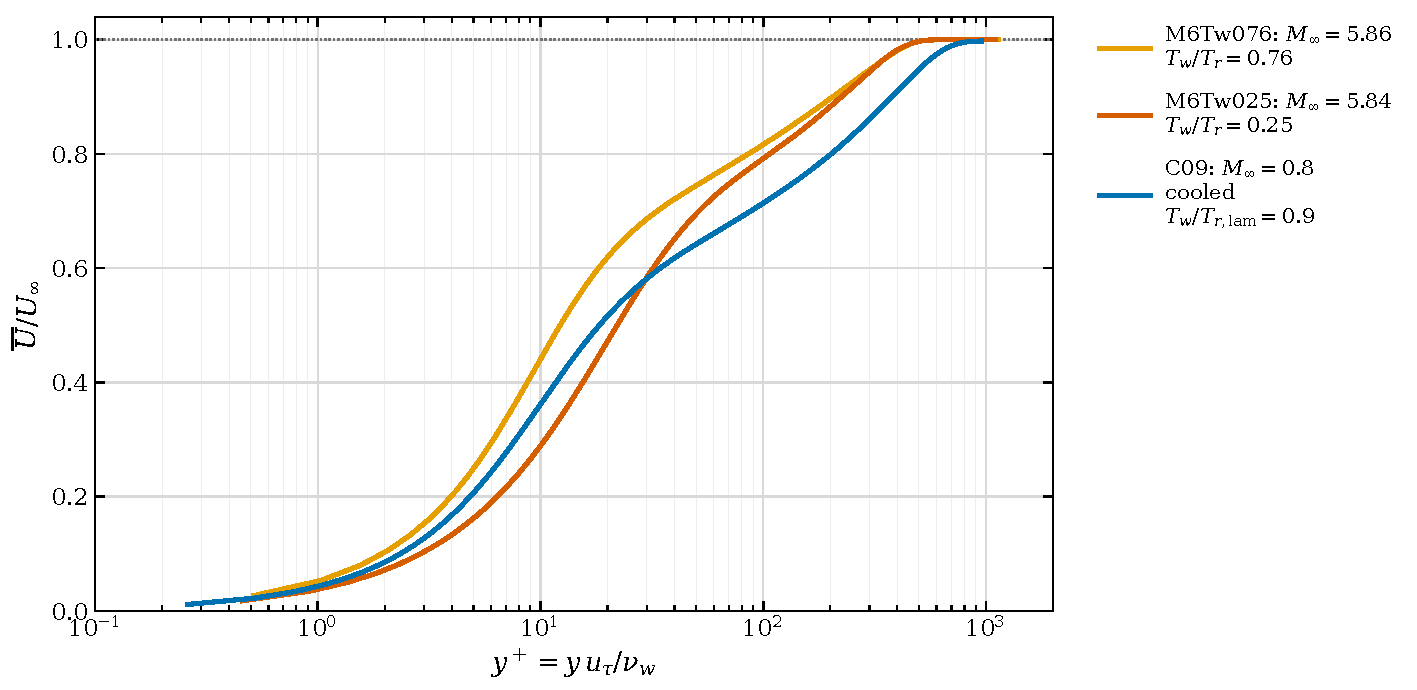
\includegraphics[width=\linewidth]{02_Background/Figures/velocity_profiles.pdf}
    \caption[DNS velocity profiles for hypersonic and subsonic turbulent boundary layers]{Freestream-normalized Reynolds-mean velocity profiles for the hypersonic M6Tw076 and M6Tw025 cases~\cite{zhang2018direct} and the fully turbulent subsonic C09 case~\cite{iwatani2025subharmonic}. All profiles use their own conventional wall units on the logarithmic \(y^+\) axis.}
    \label{fig:background:dns-velocity-profiles}
\end{figure}

\begin{figure}[H]
    \centering
    % Figure provenance:
    % Original vector export: tmp/boundary_layer_profile_comparison/temperature_profiles.pdf
    % Generating script and retained data: as for fig:background:dns-velocity-profiles.
    % Native Reynolds-mean T/Tinf columns are used for all three cases.
    % Source-sample maxima (y+, T/Tinf):
    % M6Tw025 (17.489588, 2.69037833), M6Tw076 (2.59012271, 5.46204600),
    % C09 (25.11972727, 1.02344012).
    % M6Tw076 retains the digital wall-state normalization; its discrepancy
    % from the tabulated wall temperature is discussed in the benchmark section.
    % Copied without cropping or resizing the source PDF.
    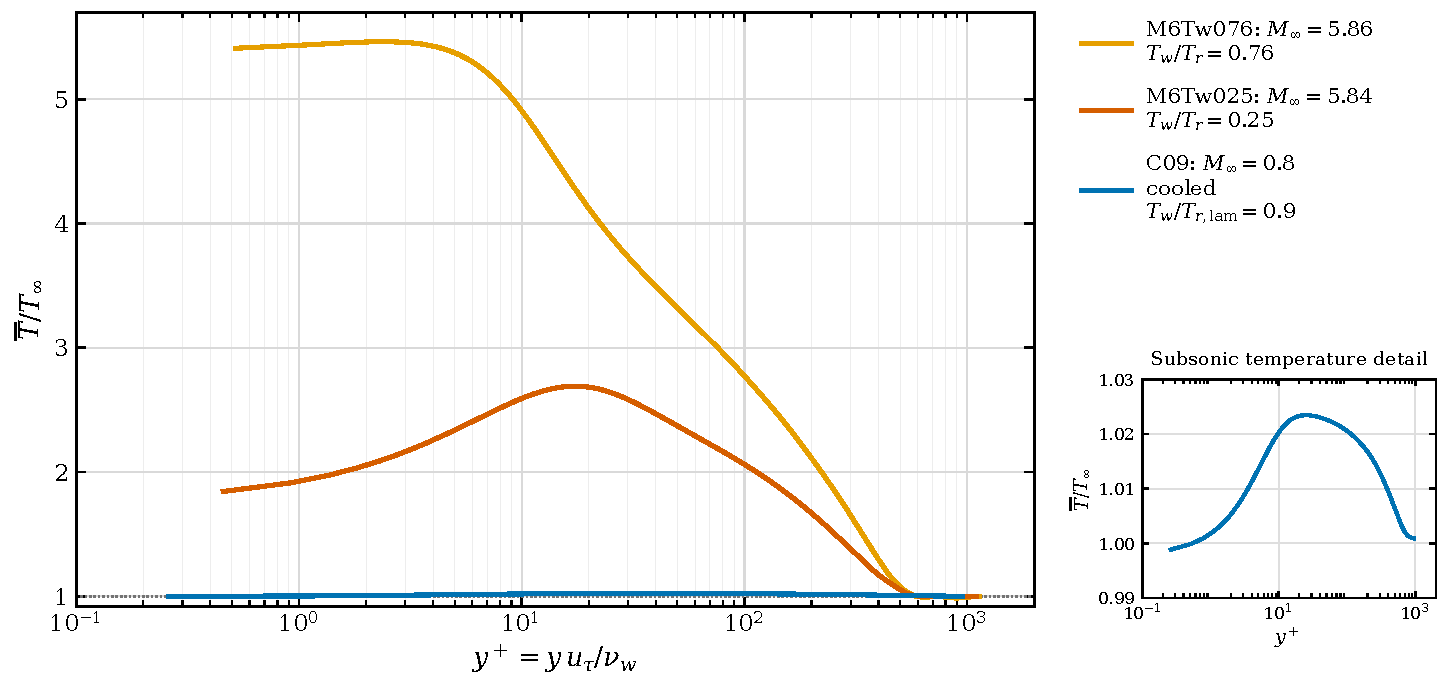
\includegraphics[width=\linewidth]{02_Background/Figures/temperature_profiles.pdf}
    \caption[DNS temperature profiles and the hypersonic cold-wall thermal maximum]{Freestream-normalized Reynolds-mean temperature profiles for the DNS cases in Figure~\ref{fig:background:dns-velocity-profiles}. The hypersonic cold-wall case M6Tw025 has a pronounced interior temperature peak, \(\overline{T}_{\max}/T_\infty\approx2.69\) at \(y^+\approx17.5\), followed by a decline towards the freestream. The near-adiabatic M6Tw076 case has only a weak near-wall maximum. The inset resolves the much smaller C09 peak, \(\overline{T}_{\max}/T_\infty\approx1.023\).}
    \label{fig:background:dns-temperature-profiles}
\end{figure}

\subsection{Compressibility and cold-wall effects and Morkovin's hypothesis}
\label{subsec:background:SRA-Morkovin}
Throughout this thesis the friction Mach number 
\begin{equation}
    M_\tau = \frac{u_\tau}{a_w},
    \qquad
    u_\tau = \sqrt{\frac{\tau_w}{\rho_w}},
\end{equation}
where \(a_w\) is the speed of sound at the wall, \(\tau_w\) the wall shear stress and \(\rho_w\) the density at the wall, is being used. The friction Mach number is discussed by Smits and Dussauge~\cite{smits2006turbulent} and is used here as an indicator for intrinsic compressibility effects, following Hasan et al.~\cite{hasan2025intrinsic}.
\par\medskip

To indicate the strength of the cold-wall effects in the used DNS references either the dimensionless wall heat-transfer rate
\begin{equation}
    B_q = \frac{q_w}{\rho_w c_p u_\tau T_w},
    \qquad
    u_\tau = \sqrt{\frac{\tau_w}{\rho_w}},
\end{equation}
with the wall heat-flux \(q_w\), wall shear stress \(\tau_w\) and heat capacity at constant pressure \(c_p\) is used. Or, as a simpler a-priori assessment, the ratio of isothermal wall temperature to adiabatic recovery temperature \(\frac{T_w}{T_r}\), e.g. \cite{zhang2018direct}.
\par\medskip

A detailed discussion of compressibility effects is beyond the scope of this work, the reader is referred to Pecnik and Hasan~\cite{pecnik2026turbulence}. Morkovin's hypothesis ~\cite{morkovin1962effects} provides a physical rationale for extending such models to compressible flow: when intrinsic compressibility effects are sufficiently small, much of the change in turbulence can be accounted for through mean-property variations \cite{fu2019turbulence}. The reference DNS studies used for assessing the turbulence models (see Section~\ref{sec:evaluation:benchmark-cases}) provide substantial support for this approximate similarity under the investigated conditions. Furthermore, the classical strong Reynolds analogy (SRA) introduces additional assumptions concerning temperature fluctuations \cite{huang2005direct}. Modified forms, including HSRA, accommodate departures from the classical relations and show approximate agreement over much of the outer boundary layer. These findings support assessing standard SA and SST formulations as compressible-flow models, but do not establish the accuracy of their momentum and thermal closures, particularly near strongly cooled walls.

\subsection{Conclusion and implications to thesis work}

The pronounced thermal-profile differences in the investigated hypersonic cold-wall case have important implications for wall-function mesh design (Section~\ref{subsec:comparative:zpg:mesh-criterion}). The linear-\(y^+\) profiles in Figures~\ref{fig:WF:dns-velocity-profiles-linear} and~\ref{fig:WF:dns-temperature-profiles-linear} relate these profile shapes to finite wall-normal spacing, because \(y^+\) is proportional to physical wall distance within each case. For wall-resolved calculations, the relevant issue is variation of the temperature gradient across the wall-to-first-cell distance: a steep but linear profile would still give an exact secant approximation to the wall derivative. Section~\ref{sec:evaluation:mesh-families-yplus} establishes the first-cell acoustic-Reynolds-number guideline through mesh-convergence studies for the investigated cases.
\section{RANS turbulence modelling}
\label{sec:background:rans-turbulence-modelling}

This section introduces the two RANS turbulence models used in this thesis, \(k\)--\(\omega\) SST and Spalart--Allmaras, and discusses their assumptions, limitations and previous assessments. The discussion focuses on aspects relevant to the present work. A comprehensive account of turbulence modelling and its rich historical development is beyond its scope. For a broader introduction, the reader is referred to David Wilcox's \emph{Turbulence Modeling for CFD}~\cite{wilcox1998turbulence}, which served as a valuable reference throughout this work.

\subsection{Menter's \texorpdfstring{\(k\)--\(\omega\)}{k–omega} SST turbulence model}

The \(k\)--\(\omega\) shear stress transport (SST) model is widely used in engineering RANS simulations. The OpenFOAM implementation follows the formulation of Menter et al.~\cite{menter2001elements}, with updated coefficients from Menter et al.~\cite{menter2003ten}. Its central feature is the blending of the Wilcox \(k\)--\(\omega\) model near the wall with a transformed standard high-Reynolds-number \(k\)-\(\varepsilon\) formulation away from the wall~\cite{menter1994two}.
\par\medskip

The validation presented in the principal SST development papers~\cite{menter1994two,menter2001elements,menter2003ten} does not include a dedicated supersonic-freestream case. Menter's original study~\cite{menter1994two} includes a transonic hump case, assessed through the surface-pressure distribution. Wilcox states that his \(k\)--\(\omega\) model can predict shock-separated flows across all Mach numbers without compressibility corrections~\cite[p.~128 and Section~5.4.7]{wilcox1998turbulence}. However, the compressible flat-plate comparisons in that discussion assess velocity profiles, leaving heat-transfer accuracy untested by those comparisons.
\par\medskip

Modifications of SST for compressible flows have since been proposed~\cite{kim2005modified,zeng2024multi,wang2024improved} and warrant further investigation. Nevertheless, SST remains widely used for hypersonic aerothermal predictions. The comparison by Hoste et al.~\cite{hoste2025review} includes NASA and DLR solvers, Ansys Fluent and STAR-CCM+ and highlights the strong reliance on the non-corrected turbulence models for aerothermal heating. Their hypersonic cone--flare results show substantial limitations in heat-transfer prediction, motivating careful assessment of the model for the flows considered here.
\par\medskip

Unless otherwise stated, the inflow turbulent-to-molecular viscosity ratio is set to\(\frac{\mu_T}{\mu}=0.001\), in accordance with the NASA Wind-US recommendation.\footnote{\url{https://www.grc.nasa.gov/WWW/winddocs/user/keywords/turbulence.html}} Preliminary sensitivity checks for the wall-resolved analysis in Section~\ref{sec:comparative:zpg:wall-resolved-baselines} found no significant changes in predicted heat-flux or boundary layer profiles when the freestream turbulence intensity \(I\) was varied. These checks are not documented in detail here and do not constitute a systematic sensitivity study.

\paragraph*{The Eddy viscosity concept}
\label{subsec:background:eddy-viscosity}

The \(k\)--\(\omega\) SST model solves two transport equations: one for the turbulent kinetic energy \(k\) and one for the specific dissipation rate \(\omega\). Together, these quantities determine the eddy viscosity. In the basic \(k\)--\(\omega\) formulation, the kinematic eddy viscosity is
\begin{equation}
    \nu_T = \frac{k}{\omega}
          = \sqrt{k}\,l_\nu,
    \qquad
    l_\nu = \frac{\sqrt{k}}{\omega}.
\end{equation}
Here, \(\sqrt{k}\) is a turbulent velocity scale and \(l_\nu\) the corresponding viscosity length scale. The SST model modifies this relation through a shear-stress limiter.
\par\medskip

Linear eddy-viscosity models use the Boussinesq hypothesis to relate the anisotropic part of the Reynolds-stress tensor to the mean strain rate through a scalar eddy viscosity. This assumption restricts the normal-stress anisotropy that the model can represent. The limitation is particularly relevant where differences in turbulent normal stresses drive secondary flows, as in three-dimensional corners.
\par\medskip

It also applies to zero-pressure-gradient flat-plate boundary layers. Under the locally parallel approximation, the Boussinesq hypothesis predicts equal turbulent normal stresses. By contrast, the flat-plate DNS of Zhang et al. used later in this work exhibit unequal normal stresses~\cite[Figure~13(a,c)]{zhang2018direct}. This discrepancy illustrates a limitation in the representation of the Reynolds-stress tensor with its consequences for mean velocity and wall shear must be assessed separately.
\par\medskip

Frahnert and Dallmann~\cite{frahnert2002examination} question the physical justification of the eddy-viscosity concept and discuss shortcomings of two-equation models even in flat-plate boundary layers. The \(k\)--\(\omega\) formulation likewise relies on modelling assumptions and dimensional reasoning~\cite[Section~4.3.1]{wilcox1998turbulence}. These limitations motivate assessing the resulting profiles and wall quantities directly, as done in Section~\ref{sec:comparative:zpg:wall-resolved-baselines}.

\subsection{Spalart--Allmaras turbulence model}

The Spalart--Allmaras (SA) model is a widely used one-equation linear eddy-viscosity model that transports a modified turbulent kinematic viscosity. Like SST, it uses the Boussinesq hypothesis and is therefore subject to the limitations of the linear eddy-viscosity assumption discussed above.
\par\medskip

The native OpenFOAM implementation cites Spalart and Allmaras~\cite{SpalartAllmaras1994}. During this work, comparison with the density-conservative formulation given by Allmaras, Johnson and Spalart~\cite{AJS2012} revealed a discrepancy in its diffusion term: placing density inside the diffusive flux introduces an additional density-gradient contribution for variable-density flow. The correction described in Section~\ref{subsec:ext:spalart-allmaras-of-correction} restores the intended continuum diffusion structure. For the investigated ZPG flat-plates, it produced no significant change in heat-flux or boundary layer profiles. Nevertheless, all SA results reported in this thesis use the corrected implementation. The discrepancy and proposed correction were also reported to the OpenFOAM developers.\footnote{\url{https://gitlab.com/openfoam/core/openfoam/-/work_items/3610}}

\subsection{Previous assessments of RANS models for hypersonic boundary layers}

The widespread use of SST and SA has prompted numerous assessments. The following selection provides context for their performance in attached hypersonic boundary layers, with particular attention to the distinction between skin-friction and heat-transfer accuracy. It is not a comprehensive review. Studies using the same ZPG flat-plate benchmarks as this thesis are discussed alongside the present results in Section~\ref{subsec:comparative:zpg:results-assessment}.
\par\medskip

Bardina et al.~\cite{bardina1997turbulence} assessed turbulence models for ten flows: seven relatively simple free-shear and ZPG boundary layer flows, and three more complex flows involving separation. Their assessment included grid-refinement studies and sensitivity to initial and boundary conditions. SST performed best overall, followed by SA, although the ranking depended on the case. For the Mach-5 adiabatic-wall ZPG flat-plate, SA gave the closest overall agreement with empirical skin-friction and velocity-profile correlations. The unmodified models performed poorly for the compressible mixing layer, while compressibility corrections improved the predictions, but the authors identified a need for further improvement in free-shear flows. They also noted difficulties in recovering flows downstream of reattachment. These findings illustrate the dependence of model performance on the flow and validation quantity. In particular, agreement for an adiabatic flat-plate does not establish heat-transfer accuracy under wall cooling.
\par\medskip

Roy and Blottner~\cite{roy2001assessment} considered a Mach-8 cold-wall ZPG flat-plate, for which SA and the Menter \(k\)--\(\omega\) model agreed well with the van Driest II skin-friction relation. This comparison tests consistency with an empirical relation and provides no direct assessment of wall heat-flux. In their Mach-20 re-entry comparison at an altitude of \(24.4\,\mathrm{km}\), SA overpredicted the turbulent wall heat-flux by approximately \(15\%\), while the Menter model predicted it to within \(40\%\) of the measurements. However, the flight measurements were taken on the leeward side at an angle of attack of \(0.14^\circ\), whereas the simulations assumed axisymmetric flow at \(0^\circ\). This difference limits how confidently the heating discrepancies can be attributed to turbulence modelling alone.
\par\medskip

The later review by Roy and Blottner~\cite{roy2006review} covers experimental validation of RANS models for two-dimensional and axisymmetric hypersonic flows within the calorically perfect-gas regime. Its recommended database spans seven geometries, including flat-plates and cylinders. The review considers 18 one- and two-equation models integrated to the wall, with detailed assessments of six extensively studied models. Across the reviewed cases, surface pressure is generally predicted more successfully than heat-transfer. This conclusion includes shock-interaction flows and should not be read as a finding restricted to attached flat-plates.

\paragraph{Van Driest II as an assessment reference}
% introduction to Van Driest II analytical skin friction and heat flux for zpg flat plates and it's limits on cold-wall cases

Van Driest II theory~\cite{van1956problem} provides a skin-friction reference in some of the turbulence-model assessments discussed in Section~\ref{sec:background:rans-turbulence-modelling}, and in the primary paper of the Li et al. wall-function~\cite{li2025WF}, as discussed in Section~\ref{sec:wall-functions:gao-li}. Combined with a Reynolds analogy, it also provides heat-transfer estimates for flat-plates. However, these estimates have documented limitations under strong wall cooling. Hopkins and Inouye~\cite{hopkins1971evaluation} reported agreement generally within about 10\% for skin-friction and, with specified recovery and Reynolds analogy factors, heat-transfer for the investigated data at \(T_w/T_r>0.3\), but found that the evaluated theories failed to reproduce the data at lower wall-temperature ratios. More recent DNS comparisons likewise reveal deficiencies in van Driest II skin-friction predictions for highly cooled walls~\cite{zhao2025revisiting}. Agreement with these correlations alone therefore does not establish the accuracy of predicted wall shear stress or heat-flux and should be taken cautiously as a sole reference value.

\subsection{Conclusions and implications for this thesis}

The literature and the wall-resolved results in Section~\ref{sec:comparative:zpg:wall-resolved-baselines} show that SA and SST can struggle to predict wall shear and heat-transfer even in attached hypersonic cold-wall boundary layers. The reviewed studies do not establish a single explanation for these deficiencies or a generally accepted correction. Reliable aerothermal prediction therefore requires further assessment and development of the turbulence and thermal closures, even for these geometrically simple flows.
\par\medskip

For the present wall-function assessment, this means that errors in the underlying RANS field must be considered alongside those introduced by the wall closure and its numerical coupling. The thesis first establishes wall-resolved baselines, then evaluates the wall-function closures on prescribed profiles (Section~\ref{sec:comparative:zpg:cross-comparison}) and examines their coupled CFD behaviour on different meshes (Section~\ref{subsec:comparative:zpg:yplus-sensitivity}). These comparisons distinguish the influences of turbulence modelling, wall-function closure and mesh resolution, while allowing for interactions between them. Together, the results identify a need to improve turbulence models, wall-function closures and the associated mesh design.
\section{RANS wall-function fundamentals}
\label{sec:background:rans-wall-function-fundamentals}

This section is a brief intro to the idea of wall-functions and the difference from the universality of the boundary layers between incompressible and compressible turbulent boundary layers. For more details the reader is encourage to read Chapter 8 - "Wall Functions" of Hanjalic and Launder's "Modelling Turbulence in Engineering and the Environment" \cite{hanjalic2022modelling} - this section is far from a complete introduction.

\subsection{Spalding's law of the wall}
\label{subsec:background:spalding}
% Writing prerequisite for Chapter 7: give the unified viscous/logarithmic law,
% its near-wall limit and the roles of kappa and the log-law intercept.

Wall functions exploit \textit{some} approximate universality of the mean velocity profile in the inner region of smooth-wall turbulent flows. The dimensionless velocity and wall-normal distance are defined as \(u^+=u/u_\tau\) and \(y^+=yu_\tau/\nu\), respectively, where \(u\) is the mean tangential velocity, \(y\) is the distance from the wall, \(\nu\) is the kinematic viscosity, and \(u_\tau=\sqrt{\tau_w/\rho}\) is the friction velocity based on the wall shear stress \(\tau_w\) and fluid density \(\rho\). For incompressible, constant-property flows under approximately equilibrium conditions, profiles expressed in these wall units follow the linear relation \(u^+=y^+\) in the viscous sublayer and a logarithmic relation in the logarithmic region (see Figure~\ref{fig:background:spaldin_law-of-the-wall}). Spalding \cite{spalding1961single} combined these limiting behaviours into a single analytical interpolation spanning the viscous sublayer, blending in the buffer layer, and logarithmic region - often referred to as the universal or Spalding's law-of-the-wall. This lack of a universal law in the buffer layer is linked to general caution of using wall-functions in this specific region of \(5 \le y^+ \le 30\). Figure~\ref{fig:background:spaldin_law-of-the-wall} illustrates this blending and compares it with DNS and the two laws relations in the sublayer and log-layer respectively. Beyond the logarithmic region of the inner region of the boundary layer is the wake region, for which again special laws, such as Cole's law-of-the-wake \cite{coles1956law}. 

Such relations provide a basis for wall functions, which infer the wall shear stress from the resolved near-wall velocity and its distance from the wall, reducing the need to resolve the steep near-wall gradients explicitly. Figure~\ref{fig:background:wf-mesh} contrasts a wall-resolved mesh with a conventional wall-function mesh whose first cell centre lies in the logarithmic region. This reduction in near-wall mesh requirement reduces the computational time by reducing the overall cell number and the stiffness of the equation by avoiding the typically thin slivered cells directly at the wall \cite{ecca2015pros}. A formulation spanning all three regions is referred to as adaptive wall-function, and permits the first cell point to lie in different parts of the inner layer. 

\begin{figure}[H]
    \centering
    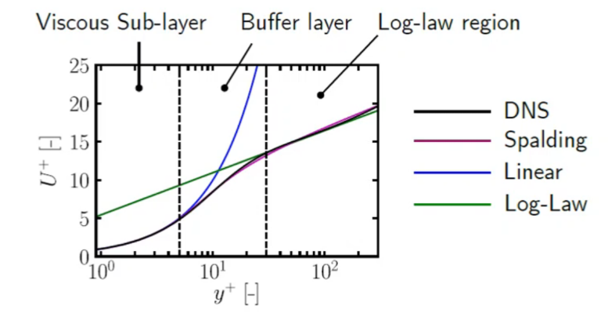
\includegraphics[width=0.7\linewidth]{02_Background/Figures/spalding_law-of-the-wall.png}
    \caption[Spalding law of the wall]{Dimensionless mean velocity profile in wall units: Spalding's law bridges the viscous sublayer, buffer layer and logarithmic region, approaching the linear and logarithmic limits. The DNS profile is shown for comparison. From \url{https://cfd.blogs.upv.es/turbulence/wall-functions/}[accessed December 2025]}
    \label{fig:background:spaldin_law-of-the-wall}
\end{figure}

\begin{figure}[H]
    \centering
    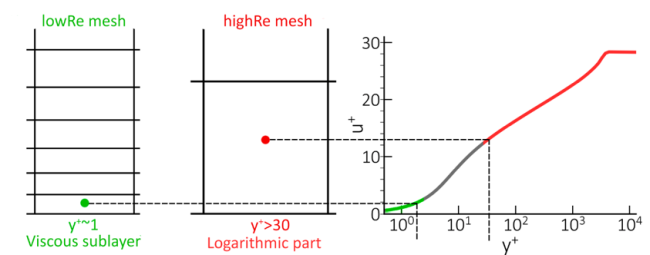
\includegraphics[width=\linewidth]{02_Background/Figures/wf_mesh.png}
    \caption[Wall-resolved and wall-function meshes]{Schematic comparison of a wall-resolved mesh (left), with its first cell centre in the viscous sublayer, and a conventional wall-function mesh (centre), with its first cell centre in the logarithmic region. The profile on the right indicates the corresponding locations in wall units. Reproduced from \url{https://ansyshelp.ansys.com/public/account/secured?returnurl=/Views/Secured/corp/v251/en/flu_th/section_kbf_dl4_vvb.html}[accessed September 2026]}
    \label{fig:background:wf-mesh}
\end{figure}

\subsection{Velocity transformations}
\label{subsec:background:velocity-transformations}
% Writing prerequisite for Chapter 7: distinguish a forward profile collapse
% from inversion of a transformation to recover wall shear at a matching point.
% State the property variations and inner-layer assumptions each law retains.

The freestream-normalized profiles in Figure~\ref{fig:background:dns-velocity-profiles} illustrate differences between the three cases, but do not directly test inner-layer similarity, which concerns \(u^+=u/u_\tau\). Compressible velocity transformations account for mean-property variations to relate the profiles to an approximately common law of the wall. Examples include the van Driest~\cite{van1951turbulent} and Trettel--Larsson~\cite{trettel2016mean} transformations, and the more recent formulations of Griffin et al.~\cite{griffin2021Transformation} and Hasan et al.~\cite{hasan2023incorporating}. Their accuracy and applicability depend on the flow conditions. The classical van Driest transformation retains \(y^+\), whereas the Trettel--Larsson and Griffin transformations use the semi-local coordinate \(y^*\). Figure~\ref{fig:background:trettel-larsson-profiles} illustrates the approximate collapse obtained with the Trettel--Larsson transformation. These transformations are not assessed individually here, the Griffin transformation is assessed indirectly through its role in the wall-function formulation~\cite{griffin2023WF}. Further discussion is given by Pecnik and Hasan~\cite{pecnik2026turbulence}.

\begin{figure}[H]
    \centering
    % Figure provenance:
    % Original vector export: tmp/boundary_layer_profile_comparison/trettel_larsson_velocity_ystar.pdf
    % Generating script: tmp/boundary_layer_profile_comparison/plot_trettel_larsson_ystar.py
    % Retained data: tmp/boundary_layer_profile_comparison/raw/
    % M6Tw076/M6Tw025: native zstar and Uvd_Trettel columns in *_Stat.dat;
    % Zhang, Duan and Choudhari (2018), DOI 10.2514/1.J057296.
    % C09: native y* and u* arrays (paper Eq. 20) from
    % https://www.klab.mech.tohoku.ac.jp/database/2025IwataniIJHFF/ustar-ystar-C09.txt
    % Iwatani, Asada and Kawai (2025), DOI 10.1016/j.ijheatfluidflow.2025.109896.
    % C09 station: Re_theta=1600, X=10.458614; differs from X=11 in earlier figures.
    % All coordinates and transformed velocities used unchanged; no C09 velocity factor.
    % Copied without cropping or resizing the source PDF.
    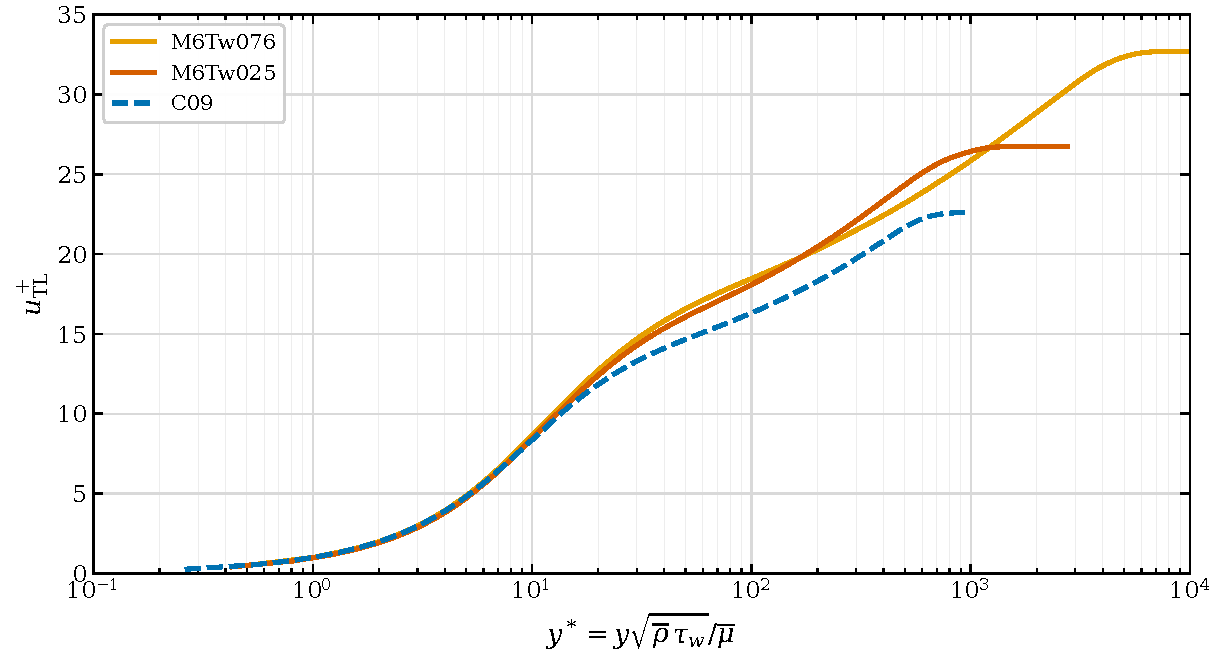
\includegraphics[width=\linewidth]{02_Background/Figures/trettel_larsson_velocity_ystar.pdf}
    \caption[Trettel--Larsson transformed DNS velocity profiles]{Trettel--Larsson transformed velocity \(u_{\mathrm{TL}}^+\) for M6Tw076 and M6Tw025~\cite{zhang2018direct} and the fully turbulent C09 case~\cite{iwatani2025subharmonic}, plotted against the semi-local coordinate \(y^*=y\sqrt{\overline{\rho}\tau_w}/\overline{\mu}\). In contrast to the freestream-normalized profiles in Figure~\ref{fig:background:dns-velocity-profiles}, the transformed profiles approximately collapse onto each other when both velocity and wall distance are transformed.}
    \label{fig:background:trettel-larsson-profiles}
\end{figure}

\subsection{Mean temperature-velocity relations - T(U)}
\label{subsec:background:temperature-velocity}
% Writing prerequisite for Chapter 7: present the mean T(U) or h(U) relations,
% their wall/reference states and cold-wall terms. Distinguish these mean
% relations (including GRA) from SRA statements about fluctuating quantities.
% Relate the wall slope to heat flux and explain the requirements for inversion.
The above mentioned velocity relation, serving as the momentum closure in wall-functions, needs a closure for the energy closure of the transport equations in the boundary layer is necessary. A similarity relation was found in the temperature-velocity relations - $T(U)$. Many of these relations exist, most notably by Crocco--Busemann, the Walz Relations \cite{walzcompressible}, by Duan-Martin \cite{duan2011direct_Part4}, or Zhang's Generalized Reynolds Analogy8 \cite{zhang2014generalized}. For a calorically perfect gas, the Crocco--Busemann and Walz relations, the Duan-Martin relation, and the mean temperature-velocity relation obtained from the generalized Reynolds analogy share a quadratic form (see Figure~\ref{fig:background:T-U-relation}). These analytical relations can be used in wall-functions to close the energy transport in the boundary layer. For the wall-function formulations investigated here, the mean \(T(U)\) relation supplies the thermal closure. Its accuracy is therefore an important additional criterion when assessing the RANS turbulence models coupled to these wall functions. It must be considered alongside \(U(y)\), \(T(y)\), their wall gradients and the resulting wall loads: agreement in \(T(U)\) alone does not establish the spatial temperature gradient, since \(\mathrm{d}T/\mathrm{d}y=(\mathrm{d}T/\mathrm{d}U)(\mathrm{d}U/\mathrm{d}y)\). Section~\ref{subsec:comparative:zpg:wr-profiles} applies these complementary assessments.

\begin{figure}[H]
    \centering
    % Figure provenance:
    % from publication: Zhang - A generalized Reynolds analogy for compressible wall-bounded turbulent flows
    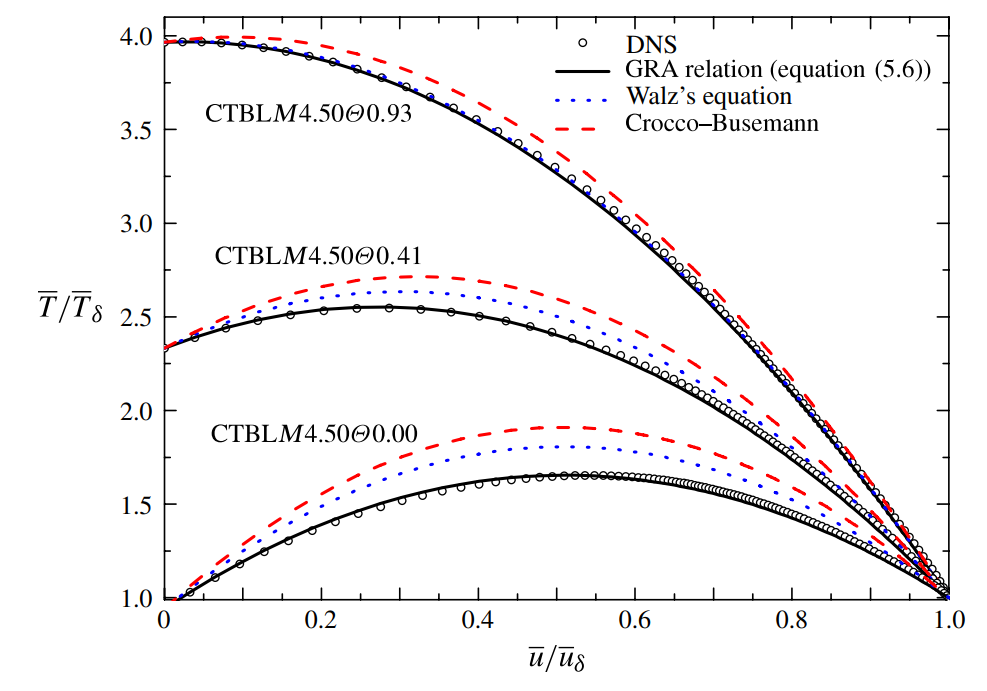
\includegraphics[width=0.85\linewidth]{02_Background/Figures/T-U-relations.png}
    \caption[introduction T(U) relations]{Mean \(T(U)\) relations for three Mach-4.5 turbulent flat-plate boundary layers with different wall thermal conditions, comparing the Crocco--Busemann, Walz and generalized Reynolds analogy relations with DNS. Reproduced from Zhang et al.~\cite{zhang2014generalized}.}
    \label{fig:background:T-U-relation}
\end{figure}


\subsection{Conclusion and implications to thesis work}

The possibility to describe the velocity and temperature boundary layer in universally similar fashion, allows for analytical descriptions of the boundary layer. With such analytical description the near-wall region need not be resolved anymore, but wall-functions based on these laws can be applied on coarse meshes. Conventional coarse wall-function meshes use a large wall-adjacent cell to span the modelled near-wall region (see Figure \ref{fig:background:wf-mesh}). The cold-wall profile shapes introduced in Section~\ref{sec:background:turbulent-boundary-layers-wall-heat-transfer} can make the associated internal-face spacing inadequate, as examined in Section~\ref{subsec:comparative:zpg:mesh-criterion}. Special formulations for the velocity and and temperature relations in hypersonic boundary layers are required, two wall-functions designed for these, by Li et al. \cite{li2025WF} and Griffin et al. \cite{griffin2023WF}, are being investigated in this thesis work (Section \ref{chap:wall-function-formulations}).

\chapter{Numerical framework}
\label{chap:numerical-framework}

This chapter introduces the OpenFOAM/HiSA framework used in this work and
summarizes the physical models, numerical methods and implementation changes
relevant to aerothermal predictions. Particular attention is given to how wall heat-flux
calculation and internal-face transport are handled, which underpin the later wall-resolved mesh
assessment and the wall-function mesh-sensitivity analysis. Complete case dictionaries, property coefficients and source modifications are documented in the repository identified in the
\hyperref[chap:data-avail]{Data Availability statement}.

\section{OpenFOAM and HiSA}
\label{sec:numerical-framework:openfoam-hisa}

\subsection{Open Field Operation And Manipulation - OpenFOAM}

\textbf{Open} \textbf{F}ield \textbf{O}peration \textbf{A}nd \textbf{M}anipulation (OpenFOAM) is an open-source\footnote{\url{https://gitlab.com/openfoam/core/openfoam}} CFD framework based on the finite volume method (FVM) and developed primarily by OpenCFD Ltd since 2004. This work uses version v2412. A relevant subsequent development is the introduction of Menter's generalized \(k\)--\(\omega\) (GEKO) turbulence model~\cite{menter2025GEKO} in OpenFOAM v2606. This model should also be considered in future turbulence-model assessments.
\par\medskip

OpenFOAM can be adapted to specific user needs through custom libraries that interact with the framework via its application programming interface (API). This allows extensions without modifying the core source code and simplifies upgrades to later versions.
\par\medskip

The FVM is the most widely used approach in CFD, adopted by commercial codes such as Ansys Fluent\footnote{\url{https://ansys.synopsys.com/products/fluids/ansys-fluent}} and research codes such as NASA's FUN3D\footnote{\url{https://fun3d.larc.nasa.gov/}} and DLR's TAU\footnote{\url{https://www.dlr.de/en/as/research-and-transfer/software-solutions/aerodynamics/software-tau}}. However, access to several solvers designed for compressible flow is restricted, including DLR's TAU, NASA's VULCAN-CFD and NASA's LAURA, the latter developed specifically for aerothermal heating.
\par\medskip

OpenFOAM has nevertheless been widely used in research, with applications and validation studies covering a broad range of flow conditions. Examples are documented in the six volumes of the OpenFOAM Journal\footnote{\url{https://journal.openfoam.com/}} published to date and in contributions to the annual OpenFOAM Workshops\footnote{\url{https://openfoamworkshop.org/}}.

\subsection{High Speed Aerodynamic solver - HiSA}
\label{subsec:numerical-framework:hisa}

The \textbf{Hi}gh \textbf{S}peed \textbf{A}erodynamic (HiSA) solver~\cite{heyns2014HiSA} is an open-source\footnote{\url{https://hisa.gitlab.io/index.html}} solver developed for OpenFOAM to provide efficient and robust simulations of high-speed, compressible viscous flows. It uses a matrix-free, implicit, coupled density-based formulation. The resulting sparse, non-symmetric linear systems are solved using the generalized minimal residual (GMRES) algorithm~\cite{saad1986gmres} with lower--upper symmetric Gauss--Seidel (LU-SGS) preconditioning~\cite{yoon1988lusgs}. This work uses HiSA version 1.12.5.
\par\medskip

HiSA has been applied to numerous cases.\footnote{\url{https://hisa.gitlab.io/doc.html}} Simulations of supersonic ejector flow~\cite{macia2019ssFlowEjector} and predictions of pressure coefficients on a missile body in supersonic flow~\cite{jun2025ssMissileBody} showed acceptable agreement with experiments. The solver has also been used to develop a compressibility-corrected \(k\)--\(\omega\) turbulence model~\cite{yin2026compressibility}. Its application to separation and heat-flux prediction around a rectangular protrusion in hypersonic flow yielded mixed results~\cite{balkhi2025rectProtrusion}.
\par\medskip

HiSA natively provides the HLLC and AUSM\(^+\)-up numerical flux schemes. This limited selection is a drawback, given the developments in the AUSM family since the introduction of AUSM\(^+\)-up in 2006~\cite{edwards2019AUSMfamily}. This work therefore uses an in-house extension of HiSA that provides an AUSMDV2\(^+\)-based scheme, as described in Section~\ref{subsec:ext:AUSM}.
\par\medskip

\paragraph*{Riemann boundary condition}
% Boundary-condition evidence:
% HiSA User Guide, July 2021, Section 2.1, pp. 11--12.
% Local source: /home/mgnadlinger/OpenFOAM/mgnadlinger-v2412/modules/hysa/
% src/finiteVolume/boundaryConditions/characteristic/characteristicWall/
% characteristicWallPressureFvPatchScalarField.C and src/modules/hisa/updateFields.H.
% Personal communication: Oliver Oxtoby to Michael Gnadlinger, 11 August 2026,
% supplied in the Outlook PDF; the email is paraphrased, not reproduced.
HiSA also provides characteristic, or Riemann-type, boundary conditions for
compressible flow. These use a linearised wave analysis to distinguish
information entering and leaving the domain. At open boundaries, incoming
information follows the prescribed external data, while outgoing information
comes from the interior solution, according to the local flow direction and
boundary-normal Mach number. The farfield formulation aims to limit
artificial reflections and are thus preferably used for supersonic flow~\cite[Section~2.1]{HeynsOxtoby2021HiSAUserGuide}. Ordinary \texttt{zeroGradient} conditions simply extrapolate interior values.
\par\medskip

At solid walls, \texttt{characteristicWallPressure} adjusts pressure using
the wall-normal velocity difference between the adjacent cell and the wall.
In personal correspondence, Oxtoby~\cite{Oxtoby2026CharacteristicWallPressure}
explained that this improves robustness when the adjacent flow has a
supersonic wall-normal component, for example near corners, where
zero-gradient pressure can become unstable. For this HiSA separately overwrites the
density stored at the wall face with the value of the first off-wall cell. It was found that especially on non-wall-resolving, coarse meshes, associated with wall-function this simplification results in unphysical wall density readings. This can have implications in post-processing or with wall-function closures that rely on the density at the wall face.

\section{Physical model and thermophysical properties}
\label{sec:numerical-framework:governing-equations}

HiSA solves the compressible conservation equations for mass, momentum and
total energy. The turbulent calculations use RANS with the eddy-viscosity and
thermal closures introduced in Section~\ref{sec:background:rans-turbulence-modelling}. The fluid is treated as a single-component or frozen-composition ideal gas, without chemical reactions. The boundary conditions and property values are chosen to represent each respective reference case and are stated in their respective section throughout this work.

\subsection{Thermophysical properties in OpenFOAM}
\label{subsec:thermophysical-properties-OF}

OpenFOAM assembles the thermophysical description from separate models for the
equation of state, caloric properties, transport properties and energy variable.
Their combination is selected in \texttt{thermophysicalProperties} and must be
registered in the installation. The \texttt{perfectGas} equation of state, \(p=\rho RT\), can be combined with constant specific heat through \texttt{hConst}, or temperature-dependent
specific heat through \texttt{janaf}. The latter uses piecewise NASA
seven-coefficient polynomials to describe the temperature dependent behaviour.
\par\medskip

Molecular viscosity \(\mu\) and thermal conductivity \(\kappa\) must reproduce
the reference laws together. Their relation is expressed by the molecular
Prandtl number, \(Pr=c_p\mu/\kappa\). In particular, the standard
\texttt{sutherland} transport model couples its viscosity law internally in OpenFOAM to a modified
Eucken conductivity relation and it is not possible to independently prescribe a constant
\(Pr\). This is a limitation of that model combination in OpenFOAM. The additional combinations described in Section~\ref{subsec:ext:thermo-physical-extension} permit separate polynomial
descriptions of \(\mu(T)\) and \(\kappa(T)\). This allows, that for the calorically perfect
benchmarks with a constant \(Pr\), the conductivity polynomial-coefficients can then be set proportional to the viscosity coefficients so that \(Pr\) can remain constant.

\subsection{Turbulent transport}

The turbulent Prandtl number \(Pr_t\) controls the modelled turbulent heat
transport and is distinct from molecular \(Pr\). With the gradient-diffusion
closure, the effective coefficients are
\(\mu_{\mathrm{eff}}=\mu+\mu_t\) and
\(\kappa_{\mathrm{eff}}=\kappa+c_p\mu_t/Pr_t\).
Unless stated otherwise, the turbulent calculations use \(Pr_t=0.9\), as
specified in Paragraph~\ref{para:turbulent-Prandtl-number}.
These effective coefficients enter both the numerical transport operations
below and the later thermal-profile assessment in
Section~\ref{subsec:comparative:zpg:wr-prandtl}.

\section{Numerical methods}
\label{sec:numerical-framework:discretization}
% Configuration provenance (WSL):
% /home/mgnadlinger/Zhang_DNS_ZPGFP/kwSST_Prt0p9/M6Tw025/system/fvSchemes
% /home/mgnadlinger/Zhang_DNS_ZPGFP/kwSST_Prt0p9/M6Tw025/system/fvSolution
% Solver source: /home/mgnadlinger/OpenFOAM/mgnadlinger-v2412/modules/hysa/
% src/finiteVolume/compactSnGradScheme/compactSnGrad.{H,C}
% src/finiteVolume/fluxSchemes/ausmDV/ausmDVFluxScheme.{H,C}

The equations are discretized by a cell-centred finite-volume method.
Fluxes across cell faces determine the discrete conservation balances.
Table~\ref{tab:numerical-framework:schemes} summarizes the numerical setup, which
unless stated otherwise, is the same numerical method used throughout this
work, with the turbulence-equation entries adapted to the selected model.
Pseudo-time Courant limits and other convergence controls are adjusted by
case. The complete settings are supplied with the simulation setups in the
\hyperref[chap:data-avail]{Data Availability statement}.

\begin{table}[htbp]
    \centering
    \small
    \caption{Numerical methods in the representative M6Tw025 configuration.}
    \label{tab:numerical-framework:schemes}
    \begin{tabular}{@{}p{0.29\linewidth}p{0.65\linewidth}@{}}
        \toprule
        Operation & Selected method \\
        \midrule
        Convective flux & AUSMDV2\(^+\)-based scheme;
            dictionary selection \texttt{AUSMDV}
            (Section~\ref{subsec:ext:AUSM}) \\
        Face-state reconstruction & Weighted van Leer limiter
            (\texttt{wVanLeer}) for density, velocity and temperature \\
        Cell gradients & Limited Gauss gradients:
            \texttt{cellLimited Gauss linear 1} \\
        Momentum and energy diffusion & \texttt{Gauss linear compact}:
            linear coefficient interpolation and HiSA's compact
            face-normal gradient \\
        Other diffusion operators & \texttt{Gauss linear corrected};
            general face-normal gradient \texttt{corrected} \\
        Turbulence convection & Bounded first-order upwind for
            turbulence properties \\
        \bottomrule
    \end{tabular}
\end{table}

\subsection{Convective and diffusive face operations}

Convective fluxes use reconstructed states on either side of each face.
The reconstruction and its limiting must be distinguished from the
face-normal gradients used for viscous stress and thermal diffusion.
\par\medskip

For an orthogonal wall-normal stencil, the compact gradient reduces to the
slope between neighbouring cell-centre values. The coefficient multiplying
that gradient is interpolated to the face with distance weighting
\begin{equation}
    D_f\phi=\frac{\phi_R-\phi_L}{h},
    \qquad
    \Gamma_f\simeq\frac{b\Gamma_L+a\Gamma_R}{h},
    \qquad
    a=y_f-y_L,\quad b=y_R-y_f,\quad h=a+b.
    \label{eq:numerical-framework:internal-face-operators}
\end{equation}
Here \(y_L\) and \(y_R\) are the neighbouring cell-centre positions, \(y_f\)
is the face position, and \(h=y_R-y_L\) is the full centre separation.
The field \(\phi\) denotes a transported quantity, such as internal energy,
and \(\Gamma\) its effective diffusion coefficient. For a perfect gas with
constant specific heat, the energy-diffusion term can equivalently be
expressed using temperature and effective thermal conductivity. On non-orthogonal
meshes, the compact scheme adds a correction using interpolated cell
gradients, but in the scope of this work all meshes are 2D, structured, orthogonal grids.
\par\medskip

For a face midway between two centres, the secant gradient has a
second-order truncation error. Unequal centre-to-face distances introduce
an additional asymmetry term. Thus, neither the nominal order nor the
wall-function sampling height alone establishes the accuracy of an
internal-face flux. The cold-wall profile analysis in
Section~\ref{subsec:comparative:zpg:mesh-criterion} examines these gradient
and coefficient-interpolation operations and their implications.

\section{Wall heat-flux and shear stress}
\label{sec:openFOAM_qw_tauw}

Wall heat-flux and shear stress depend on local derivatives, so their numerical evaluation is part of the near-wall resolution requirement. This section describes the standard OpenFOAM evaluation of heat-flux and shear stress.

\subsection{Heat-flux and effective thermal transport}

% Implementation evidence (OpenFOAM v2412):
% /opt/of-v2412/src/functionObjects/field/wallHeatFlux/wallHeatFlux.C
% /opt/of-v2412/src/thermophysicalModels/basic/heThermo/heThermo.C
% /opt/of-v2412/src/TurbulenceModels/compressible/EddyDiffusivity/EddyDiffusivity.C
% HiSA energy residual:
% /home/mgnadlinger/OpenFOAM/mgnadlinger-v2412/modules/hysa/src/modules/hisa/residualsUpdate.H
The \texttt{wallHeatFlux} function object in OpenFOAM evaluates the effective energy diffusivity multiplied by the outward-normal gradient of sensible internal energy in the present HiSA setup. With radiation omitted,
\begin{equation}
    q_w^{\mathrm{OF}}
    = \alpha_{\mathrm{eff},w}\left.\frac{\partial e}{\partial n_{\mathrm{out}}}\right|_w,
    \qquad
    \alpha_{\mathrm{eff}}
    = \frac{c_p}{c_v}(\alpha+\alpha_t),
    \qquad
    \alpha=\frac{\kappa}{c_p}.
    \label{eq:q_w_openFOAM_math}
\end{equation}
Here \(e\) denotes sensible internal energy and \(c_v\) the specific heat at constant volume. The field \texttt{alphat} stores \(\alpha_t\), the turbulent contribution to heat transport. It is related to the kinematic eddy viscosity \(\nu_t\), stored as \texttt{nut}, through the turbulent Prandtl number \(Pr_t\):
\begin{equation}
    Pr_t=\rho\,\frac{\nu_t}{\alpha_t}.
    \label{eq:openfoam-alphat-nut}
\end{equation}
Here \(\rho\) is the fluid density.
\par\medskip

For constant specific heats, a fixed wall temperature and an orthogonal wall-adjacent cell, the discrete expression for the wall-heat-flux thus becomes
\begin{equation}
    q_w^{\mathrm{OF}}
    = \kappa_{\mathrm{eff},w}\frac{T_w-T_1}{y_1},
    \qquad q_w=-q_w^{\mathrm{OF}}.
    \label{eq:q_w_openFOAM_simple}
\end{equation}
The distance \(y_1\) is measured from the wall face to the first cell centre.

\subsection{Shear stress and effective viscosity}

% Implementation evidence:
% /opt/of-v2412/src/functionObjects/field/wallShearStress/wallShearStress.C
% /opt/of-v2412/src/TurbulenceModels/turbulenceModels/linearViscousStress/linearViscousStress.C
The \texttt{wallShearStress} function object in OpenFOAM calculates wall shear stress from the velocity gradient and effective viscosity. For a flat, stationary no-slip wall, the tangential stress acting on the fluid is approximated by
\begin{equation}
    \boldsymbol{\tau}_{w,t}^{\mathrm{OF}}
    \simeq -\mu_{\mathrm{eff},w}\frac{\boldsymbol{U}_{1,t}}{y_1},
    \qquad
    \mu_{\mathrm{eff}}=\mu+\rho\nu_t.
    \label{eq:tau_w_openFOAM_simple}
\end{equation}
It opposes the tangential fluid velocity. From the shear stress \(\tau_w\), the skin-friction coefficient \(C_f\) is obtained by normalizing this stress with the specified reference dynamic pressure. In wall-resolved simulations, the turbulent contributions vanish at the wall. Wall shear stress and heat-flux therefore depend on the molecular transport coefficients and the resolved temperature and velocity gradients only.

\subsection{Implications for mesh resolution}

Equations~\eqref{eq:q_w_openFOAM_simple} and~\eqref{eq:tau_w_openFOAM_simple} use a wall-to-cell secant to approximate the wall derivative. This one-sided approximation is generally first-order accurate at the wall, even when the internal-face discretization is second-order accurate. A small nominal \(y_1^+\) alone does not establish that the secant represents the wall slope. Section~\ref{sec:evaluation:mesh-families-yplus} assesses the required first-cell spacing through mesh-convergence studies.
\par\medskip

A wall function instead supplies modelled wall heat-flux and shear stress from a sampled boundary layer state. Their direct substitution into HiSA, described in Section~\ref{subsec:wall-functions:direct-flux-delivery}, avoids the wall-gradient approximation above. Transport across internal faces still depends on the numerical methods in Section~\ref{sec:numerical-framework:discretization}, the resulting mesh sensitivity is examined in Section~\ref{subsec:comparative:zpg:mesh-criterion}.

\section{Extensions and corrections to the framework}
\label{sec:numerical-framework:extensions}

The framework was extended to support the chosen convective flux,
reference-consistent molecular transport and additional convergence
diagnostics. A separate correction addresses the variable-density SA
formulation. The following descriptions identify the purpose and scope of
each change. Their source is supplied through the
\hyperref[chap:data-avail]{Data Availability statement}.

\subsection{HiSA extension with \texorpdfstring{AUSMDV2\(^+\)}{AUSMDV2+}}
\label{subsec:ext:AUSM}
% Source provenance (WSL):
% /home/mgnadlinger/OpenFOAM/mgnadlinger-v2412/modules/hysa/src/finiteVolume/
% fluxSchemes/ausmDV/ausmDVFluxScheme.{H,C}
% TypeName("AUSMDV"); AUSMDV2+ blending with locally modified pressure flux.

The in-house HiSA extension provides an AUSMDV2\(^+\)-based flux scheme,
selected as \texttt{AUSMDV} in the case dictionaries. It blends AUSMD\(^+\)
and AUSMV\(^+\) contributions following
Phongthanapanich and Matthujak~\cite{PhongthanapanichMatthujak2021AUSMDV2Plus}.
The scheme was selected for shock resolution and robustness. The
stand-off-distance study in
Section~\ref{sec:numerical-vv:shock-stand-off-carbuncle} assesses this
implemented variant and documents its remaining carbuncle sensitivity.
The later boundary layer assessment separately examines the viscous
transport operations introduced in
Section~\ref{sec:numerical-framework:discretization}.

\subsection{Additional thermophysical-model combinations}
\label{subsec:ext:thermo-physical-extension}
% Source provenance (WSL):
% /home/mgnadlinger/OpenFOAM/mgnadlinger-v2412/src/myThermos/myThermos.C

Matching the DNS references requires independent control of the molecular
viscosity and conductivity laws. The user library \texttt{myThermos}
registers OpenFOAM's existing polynomial transport model with the ideal-gas
equation of state, sensible internal energy, and either constant or
temperature-dependent specific heat. It enables these combinations without
changing the underlying property models.
\par\medskip

For the calorically perfect benchmarks, seventh-order polynomials represent
the prescribed viscosity laws, and proportional conductivity coefficients
enforce the selected constant molecular Prandtl number. The fits are checked
over the temperatures encountered in each simulation.
Section~\ref{sec:evaluation:benchmark-cases} documents the reference laws
and fit assessment.

\subsection{Density-gradient correction to Spalart--Allmaras}
\label{subsec:ext:spalart-allmaras-of-correction}

The OpenFOAM v2412 SA implementation places density inside the diffusive
flux of its transported working variable. For variable density, this
introduces an additional density-gradient term relative to the
material-form SA equation~\cite{SpalartAllmaras1994,AJS2012}.
The custom \texttt{SpalartAllmarasDensityCorrected} model cancels that term
while retaining the other components of the local implementation.
Appendix~\ref{app:spalart-allmaras-density} gives the derivation and source
audit. This correction restores the intended continuum diffusion structure and is subsequently used as the only SA model being assessed in Section~\ref{sec:comparative:zpg:wall-resolved-baselines}.
\section{Convergence assessment and reproducibility}
\label{sec:numerical-framework:convergence}

Iterative convergence concerns changes in the solution on a fixed mesh, while
mesh convergence concerns changes under spatial refinement. Both must be
assessed before differences from a physical reference can be attributed to
the flow model.

\subsection{Iterative convergence}
% Evidence (WSL):
% /home/mgnadlinger/Zhang_DNS_ZPGFP/kwSST_Prt0p9/M6Tw025/log.hysa
% /home/mgnadlinger/Zhang_DNS_ZPGFP/kwSST_Prt0p9/M6Tw025/M6Tw025_summary.md
% Final-window check: 21 records over iterations 14000--15000 from
% postProcessing/wallHeatFlux_areaAverage/0/surfaceFieldValue.dat and
% postProcessing/wallShearStress_areaAverage/0/surfaceFieldValue.dat.
% 100*(max-min)/abs(mean): heat flux 0.0012917%, shear 0.0013894%.
% Shear operation is magnitude AFTER vector area averaging.
% GMRES normalization source: modules/hysa/src/solvers/gmres/
% gmresTemplates.C (normalized sums of absolute equation residuals).

The assessment combines residual histories with the evolution of physical
outputs. HiSA reports normalized sums of absolute residuals for continuity,
momentum and total energy. These are inspected together with the
turbulence-equation residuals. For flat-plates, the monitored physical outputs include the
wall-averaged heat-flux and the magnitude of the wall-averaged shear vector. It is important to note that besides extrema and averages, it was seen to also be crucial to track the coefficient of variance of the tracked field to assess convergence, as extrema or averages can hide when adjacent cells are still balancing out.

\subsection{Mesh convergence and numerical uncertainty}

The mesh studies use the E\c{c}a--Hoekstra
procedure~\citep{EcaHoekstra2014NumericalUncertainty}, which fits systematically
refined solutions by least squares and accommodates scattered or
non-monotonic refinement data. It shares the extrapolation basis of the
Grid Convergence Index~\citep{Roache1994GridRefinement} and the procedure of
Celik et al.~\citep{Celik2008DiscretizationUncertainty}.
The fit estimates the zero-spacing result \(\phi_0\) and an uncertainty
\(U_{\mathrm f}\) for the finest-grid result \(\phi_{\mathrm f}\), with a
safety factor dependent on the observed convergence behaviour.
\par\medskip

Where an independent reference \(\phi_{\mathrm{ref}}\) is available, the
signed errors and normalized finest-grid uncertainty are reported as
\begin{equation}
    e_j=100\frac{\phi_j-\phi_{\mathrm{ref}}}{\phi_{\mathrm{ref}}},
    \quad j\in\{\mathrm f,0\},
    \qquad
    u_{\mathrm f}=100\frac{U_{\mathrm f}}{|\phi_{\mathrm f}|}.
    \label{eq:numerical-framework:error-uncertainty}
\end{equation}
The uncertainty estimates spatial-discretization effects and presupposes
that iterative and round-off errors are sufficiently small. It does not
measure agreement with DNS or account for turbulence-model error.
The wall-resolved mesh choices are justified in
Section~\ref{sec:evaluation:mesh-families-yplus}, with the full convergence
results in Appendix~\ref{app:zpg:mesh-convergence}.

\subsection{Reproducibility}

The \hyperref[chap:data-avail]{Data Availability statement} identifies the
repository containing the simulation configurations and supporting data.
The case dictionaries specify the numerical schemes, solution controls,
physical properties and boundary conditions. The accompanying source
modifications and processing scripts document how the reported wall loads
and comparisons are obtained. Case-specific departures from the common
setup are stated with the corresponding assessment.


\include{04_OpenFOAM_HiSA_VnV/00_openFoam_HiSA_VnV}
\chapter{Wall-function formulations and implementation}
\label{chap:wall-function-formulations}

The investigated wall functions combine momentum and thermal closures to infer wall shear stress and heat-flux from a sampled boundary layer state. Figure~\ref{fig:WF:wall-function-idea-illustration} shows this coupling: the sampled velocity and thermodynamic state, the physical wall temperature and the required reference information determine the wall loads. Their delivery to the CFD equations is distinct from the closure itself. Coupling to a RANS turbulence model additionally requires a compatible near-wall turbulence constraint.

\begin{figure}[H]
    \centering
    % Preserve the supplied raster diagram and typeset its wall label consistently.
    % Coordinates are relative to the 964 x 321 pixel source image.
    \begingroup
    \setlength{\unitlength}{\linewidth}
    \begin{picture}(1,0.33299)
        \put(0,0){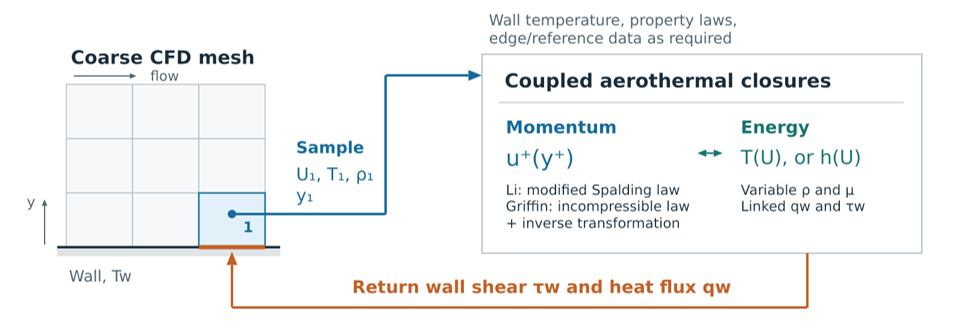
\includegraphics[width=\linewidth]{05_WF_Idea_Implementation/Wallfunction_Idea.png}}
        \put(0.0674,0.0342){\textcolor{white}{\rule{0.0778\unitlength}{0.0228\unitlength}}}
        \put(0.0716,0.0467){\makebox(0,0)[l]{\fontsize{8}{9.6}\selectfont\textcolor[RGB]{82,104,121}{Wall, \(T_w\)}}}
    \end{picture}
    \endgroup
    \caption{Wall-function coupling using the first cell as the sample. Momentum and thermal closures infer wall shear stress and heat-flux from the sampled state and the wall and reference conditions, and return these loads to the CFD solver.}
    \label{fig:WF:wall-function-idea-illustration}
\end{figure}

\section{Wall-function sampling and mesh geometry}
\label{subsec:wall-functions:sampling-geometry}

The wall-function sampling height is denoted by \(y_s\), and the wall-to-first-cell-centre distance by \(y_1\). On a conventional wall-function mesh, the first cell supplies the sample, so \(y_s=y_1\). Increasing the first-cell height consequently moves the sample outwards and coarsens the neighbouring internal-face stencils (Figure~\ref{fig:WF:wall-function-conventional-mesh}). The term \emph{conventional coarse wall-function mesh} refers to this coupled change in sampling height and mesh spacing throughout this work.

\begin{figure}[H]
    \centering
    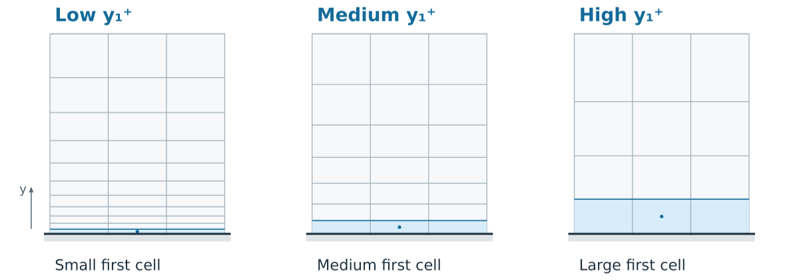
\includegraphics[width=\linewidth]{05_WF_Idea_Implementation/Wallfunction_Meshes.png}
    \caption{Conventional wall-function mesh strategy. Enlarging the wall-adjacent cell increases both the first-cell sampling height \(y_s=y_1\) and the spacing of the nearby internal-face stencils. The indicated wall-unit heights refer to the cell centres, not the full cell heights.}
    \label{fig:WF:wall-function-conventional-mesh}
\end{figure}

The implemented Li and Griffin wall functions can also sample an interior cell while retaining finer cells below it. The selected cell supplies the closure inputs and its wall-normal distance supplies \(y_s\), denoted \(y_m\) in Griffin's formulation. The associated SA constraint is applied at that same cell, while the predicted loads are delivered at the physical wall. The cells below the sample remain part of the CFD solution. This option separates closure sampling from the first-cell distance \(y_1\) and the centre separation \(h\) across an internal face at \(y_f\), defined in Equation~\eqref{eq:numerical-framework:internal-face-operators}. Because the wall loads are inferred from modelled wall slopes, the sample need not meet the wall-resolved secant requirement of Section~\ref{sec:openFOAM_qw_tauw}. Its location must nevertheless lie within the closure's applicable range. Moreover, prescribing the wall loads does not replace internal-face gradient reconstruction or transport-coefficient interpolation. Section~\ref{subsec:comparative:zpg:informed-mesh} uses the independent sampling option to assess the additional mesh requirement within the retained boundary layer. The following section first explains the common flux-delivery mechanism and subsequent sections present the individual closures and their RANS coupling.

\section{Wall-flux delivery in OpenFOAM/HiSA}
\label{sec:openFOAM_wall_function_implementation_general}

The standard wall-load evaluation in Section~\ref{sec:openFOAM_qw_tauw} combines a wall-to-cell gradient with an effective transport coefficient. Encoding a wall-function target through that coefficient is convenient, but constrains which loads can be delivered. This section motivates the direct wall-flux interface used for the investigated closures.

\subsection{Limitations of transport-coefficient boundary conditions}

A conventional implementation adjusts wall \texttt{nut} and \texttt{alphat} until the discrete gradient produces the target stress or heat-flux. For example, inversion of the planar-wall shear relation gives
\begin{equation}
    \nu_{t,w}
    =\frac{\tau_{w,\mathrm{target}}y_1}{\rho_w U_{1,t}}-\nu_w,
    \label{eq:nut_BC}
\end{equation}
where \(U_{1,t}>0\) denotes the tangential velocity magnitude. An analogous inversion determines the thermal coefficient from the target heat-flux and the wall-to-cell energy difference.

Requiring non-negative turbulent transport leaves the molecular contribution as the smallest representable flux magnitude for a given nonzero secant. It also fixes the flux direction to that of the secant. Neither condition is guaranteed to agree with a wall-function target. The thermal restriction is particularly relevant to non-monotonic temperature profiles: if a sample beyond the temperature maximum is colder than the wall while the physical wall remains cooled, a non-negative conductivity cannot deliver the required heat-flux through that wall-to-cell temperature difference. Even when the signs agree, the target can lie below the molecular secant contribution. These are limitations of the delivery mechanism, separate from closure accuracy.

\subsection{Limitations of a prescribed-gradient temperature condition}

A prescribed-gradient temperature condition can represent either heat-flux sign, but matching the target through the discrete gradient lets the patch temperature depart from the physical wall temperature used by the closure. On a coarse mesh, the resulting extrapolated face state can differ substantially from that physical state. Evaluating density and viscosity at this numerical face temperature then changes the wall transport properties and can make the molecular shear contribution exceed the target in Equation~\eqref{eq:nut_BC}. This approach therefore introduces an additional coupling between thermal flux delivery and momentum transport. Retaining the physical prescribed wall temperature while replacing the wall flux avoids this inconsistency.

\subsection{Direct wall-flux substitution}
\label{subsec:wall-functions:direct-flux-delivery}

% Implementation evidence:
% /home/mgnadlinger/OpenFOAM/mgnadlinger-v2412/modules/hysa/src/modules/hisa/wallFluxSubstitution.H
% /home/mgnadlinger/OpenFOAM/mgnadlinger-v2412/src/LiWallFunctions/DESIGN_AND_DEVIATIONS_LiFlux.md
% /home/mgnadlinger/OpenFOAM/mgnadlinger-v2412/src/GriffinWallFunctions/DESIGN_AND_DEVIATIONS_GriffinFlux.md
% Reporting verified against:
% /home/mgnadlinger/WF_validation/LowH_M3/validation/scripts/plot_wall_flux_sweeps.py
% /home/mgnadlinger/WF_validation/LowH_M3/validation/scripts/plot_opt_mesh_wall_flux_sweeps.py
The implemented interface replaces the explicit viscous wall-face contributions in HiSA's momentum and total-energy residuals. Each wall function publishes its target traction, target heat-flux and an active-face mask. HiSA first assembles the standard wall contributions, then adds the difference between the targets and those contributions on active faces. In a common convention, with traction acting on the fluid and heat-flux \(q_w\) positive into the wall, the corrections per unit area are
\begin{equation}
    \Delta\boldsymbol{\tau}
    =\boldsymbol{\tau}_{w,\mathrm{target}}-\boldsymbol{\tau}_{\mathrm{std}},
    \qquad
    \Delta q=-q_{w,\mathrm{target}}-q_{\mathrm{std}}.
    \label{eq:wall-functions:flux-substitution}
\end{equation}
The standard terms are the actual terms assembled by HiSA, including the full viscous traction and \(q_{\mathrm{std}}\) is positive into the fluid, following OpenFOAM's convention. The target traction is tangential, as assumed by the boundary layer wall closures. The energy correction includes the corresponding viscous work, which vanishes at a stationary no-slip wall. Inactive faces retain the standard evaluation.

For the isothermal cases, this interface keeps the physical fixed wall temperature and sets wall \texttt{nut} and \texttt{alphat} to zero; these fields no longer encode the target loads. The near-wall turbulence constraint remains a separate part of the RANS coupling. Direct substitution changes neither the wall-function closure nor the internal-face transport operators, and does not impose an exact off-wall profile. It removes the coefficient-inversion restriction while leaving closure error, turbulence-model error and spatial-discretization error to be assessed in Chapter~\ref{chap:comparative-evaluation}.

The imposed loads are recorded in the wall-function diagnostics. Li's native heat-flux is positive into the wall, whereas Griffin's and Wang's are positive into the fluid; the interface and comparison scripts convert these signs consistently. Standard \texttt{wallHeatFlux} and \texttt{wallShearStress} function objects do not include the residual correction and therefore do not report the imposed targets. The coupled wall-function comparisons use the diagnostic targets on active faces; the wall-resolved comparisons use the standard function-object output. The source code and case configurations are identified in the \hyperref[chap:data-avail]{data-availability statement}.

\section{Li wall function}
\label{sec:wall-functions:gao-li}

Li et al. developed an improved wall function for hypersonic reacting turbulent boundary layers, addressing strong wall cooling and variable gas properties~\cite{li2025WF}. Their comparison with the precursor formulation of Gao et al. shows substantially smaller skin-friction and heat-flux errors for the investigated cold-wall flat-plates~\cite[Section~IV.B, Figures~17--20]{li2025WF}. The improvements concern both the thermal relation and the treatment of variable properties in the velocity law. This motivates investigating the Li formulation here, while the earlier Gao formulation is not additionally being evaluated.

\subsection{Momentum and thermal closures}
\label{subsec:wall-functions:gao-li:governing-relations}

The thermal closure is a quadratic relation between static enthalpy and velocity~\cite[Eqs.~(12)--(15)]{li2025WF}. It extends the generalized temperature--velocity relation of Zhang et al. by using enthalpy to accommodate reacting-gas thermodynamics. Its generalized recovery enthalpy determines the wall slope and thereby relates heat-flux to wall shear, extending the fixed-recovery-factor prescription of the earlier Walz-based construction.
\par\medskip

The momentum closure combines a viscosity-corrected viscous-sublayer relation with a compressible logarithmic law in a unified expression~\cite[Eqs.~(27), (30)--(32)]{li2025WF}. It assumes approximately constant total shear stress in the inner layer and blends through the buffer layer. Sampling below the logarithmic region is therefore permitted by construction, although accuracy can still vary with sampling height.
\par\medskip

\label{subsec:wall-functions:gao-li:empirical-constants}
The formulation retains \(\kappa=0.41\) and \(B=6.0\) and approximates the viscosity variation by an enthalpy power law. Li et al. fit its exponent, denoted \(\omega_H\) here, to approximately \(0.72\) in their reacting viscous-sublayer profiles~\cite[Eq.~(25) and Figure~12]{li2025WF}. This transport approximation is calibrated for those conditions; its transfer to other gas models and wall temperatures is not automatically given and open to scrutiny.

\subsection{Non-reacting implementation and reference-state choice}
\label{subsec:wall-functions:gao-li:openfoam-implementation}

The present implementation uses fixed composition and omits chemical reactions and species-diffusion contributions. The enthalpy-based closure is retained. With the additional calorically perfect-gas assumption, \(h=c_pT\), its thermal relation reduces to the Zhang temperature--velocity relation reproduced by Li et al.~\cite[Eqs.~(8)--(13)]{li2025WF}. This equivalence concerns the thermal closure; the momentum closure remains Li's unified velocity law. Removing chemistry alone does not require constant specific heat.
\par\medskip

A useful feature is that the reference velocity and enthalpy need not be taken at the boundary layer edge. Li et al. reformulate both closures using an interior reference point and select the second off-wall grid point in their implementation~\cite[Section~IV.C, Eqs.~(40)--(42)]{li2025WF}. Here, the matching cell and a second cell farther from the wall provide the two velocity--enthalpy states. Together with the physical wall state, they determine the thermal relation. The unified velocity law is then inverted for the wall shear at the matching height, and the inferred thermal wall slope supplies the heat-flux. A prescribed-edge option is retained for comparison.
\par\medskip

This local reference construction avoids explicit edge detection, whose mesh-dependent reconstruction introduces additional sensitivity into Griffin's closure inputs (Section~\ref{subsec:wall-functions:griffin:edge-detection}). The second reference point remains distinct from the matching point; neither location should be confused with the full height of the wall-adjacent cell.
\par\medskip

\label{subsec:wall-functions:gao-li:turbulence-coupling}
The recovered shear stress and heat-flux are delivered directly to HiSA (Section~\ref{subsec:wall-functions:direct-flux-delivery}). Following Li et al.~\cite[Eqs.~(36)--(39)]{li2025WF}, the velocity-law derivative also supplies a compatible eddy viscosity and hence a constraint on the SA variable at the selected near-wall layer. This turbulence constraint is separate from prescribing the wall fluxes.

\subsection{Scope of the published assessment}
\label{subsec:wall-functions:gao-li:published-results}

The non-reacting flat-plate case in Li et al. checks the underlying solver and SA model against an experimental data and van Driest II theory~\cite[Section~IV.B and Figure~2]{li2025WF}. There it does not assess the improved wall function. The latter is tested on reacting flat-plates against resolved RANS solutions; the second-reference-point variant is demonstrated at first-point \(y^+=4\) and \(8\), whereas the coarser logarithmic-layer tests use edge quantities~\cite[Sections~IV.B--C]{li2025WF}. These results do not provide an independent DNS or experimental validation of the non-reacting wall function used here and can thus not be used as a way to validate the code implementation.
\par\medskip

Direct reproduction also requires care because Li et al. use a finite-difference solver. They define the wall distance to the first off-wall grid point, while their coupling acts on viscous fluxes between that point and the wall~\cite[Section~II.A, Eq.~(17) and Figure~16]{li2025WF}. Transfer to a finite-volume method requires matching the physical sampling and flux locations; equal reported \(y^+\) values alone do not establish an equivalent discretization. The published results therefore provide context rather than a direct verification case for the complete implementation.

\subsection{Reference sensitivity and assessment in this thesis}
\label{subsec:wall-functions:gao-li:limitations}

Avoiding edge detection does not remove all reference-state sensitivity. Inferring the thermal relation becomes poorly conditioned when the sampled and reference velocities nearly coincide, and both points must remain within the region represented by the closure. The prescribed-profile tests in Section~\ref{subsec:erriso:apriori-results} compare the second-point and prescribed-edge choices on the M6Tw025 DNS profile and the LowH\_M3 resolved SA profile. They show no systematic loss of accuracy from using the second point, supporting this practical advantage while retaining appreciable closure errors. These tests establish the standalone closure response before the coupled mesh sensitivity is examined in Section~\ref{subsec:comparative:zpg:yplus-sensitivity}.


\section{Griffin inverse-transformation wall function}
\label{sec:wall-functions:griffin}

Griffin et al. construct a compressible near-wall profile by applying an inverse velocity transformation to an incompressible wall law and closing the temperature profile through an algebraic temperature--velocity relation~\cite{griffin2022WFbrief,griffin2023WF}. The formulation accounts for density and viscosity variations associated with wall cooling while retaining a unified description of the viscous sublayer, buffer layer and logarithmic region. Its application here as a RANS wall function requires both the local matching state and information about the boundary layer edge.

\subsection{Momentum and thermal closures}
\label{subsec:wall-functions:griffin:governing-relations}

The momentum closure builds on the total-stress velocity transformation of Griffin et al.~\cite[Eqs.~(4)--(5)]{griffin2021Transformation}. It combines viscous scaling near the wall with turbulence-equilibrium scaling in the logarithmic region, blending between them through the buffer layer. The wall model uses its approximately constant-total-shear-stress form. Inverting this transformation converts the mean shear of a damped incompressible eddy-viscosity model into the compressible velocity gradient, including local density and viscosity variations~\cite[Eq.~(2.2)]{griffin2023WF}. The viscous limit recovers the linear wall law; the model is therefore not restricted by construction to logarithmic-layer sampling.
\par\medskip

The thermal closure is a quadratic temperature--velocity relation based on the generalized Reynolds analogy~\cite[Eq.~(2.5)]{griffin2023WF}. It satisfies the wall temperature and the sampled temperature at the matching velocity, while its wall slope is prescribed through the Reynolds analogy factor and the recovery temperature. The latter depends on the edge velocity and temperature. This wall slope links heat-flux directly to wall shear, without solving a separate temperature equation with an assumed constant turbulent Prandtl number. In Griffin's convention, heat-flux is positive into the fluid and negative for a cooled wall.
\par\medskip

For a prescribed wall temperature, the inputs are the velocity, temperature and density at the physical matching height \(y_m\), the edge state, an equation of state and a viscosity law. The inner reconstruction uses the ideal-gas law with approximately constant pressure and constant specific heat. A trial wall shear stress is used to integrate the inverse relation from the wall region to \(y_m\), updating temperature and transport properties along the reconstructed profile. The stress is iterated until the integrated velocity reproduces the sampled velocity; the thermal relation then supplies the heat-flux~\cite[Section~2.3]{griffin2023WF}. Both wall loads thus follow from reconstructed wall slopes rather than a wall-to-cell secant.
\par\medskip

The implementation retains the Reynolds-number-dependent calibration of the incompressible coefficients \(\kappa\) and \(A^+\) from the earlier research brief~\cite[Section~2]{griffin2022WFbrief}. These coefficients are selected using the edge-based semi-local friction Reynolds number, so the estimated thickness also enters the closure. The journal article examines this calibration but adopts fixed values \(\kappa=0.41\) and \(A^+=17\) for its subsequent simulations~\cite[Section~3]{griffin2023WF}. This distinction matters when comparing the implemented variant with published results.

\subsection{Boundary layer edge reconstruction and sensitivity}
\label{subsec:wall-functions:griffin:edge-detection}
\label{para:Griffin-BL-edge}

The edge quantities are obtained with Griffin et al.'s local-reconstruction method~\cite{griffin2021BLthickness}. It reconstructs a local inviscid velocity \(U_I\) from the stagnation enthalpy and identifies \(\delta_{99}\) where the actual tangential velocity first satisfies \(U/U_I=0.99\)~\cite[Eq.~(9) and Appendix~D, Eqs.~(D1)--(D2)]{griffin2021BLthickness}. This replaces comparison with a prescribed freestream velocity and permits a varying inviscid outer profile. The compressible construction assumes an inviscid, non-heat-conducting outer flow.
\par\medskip

In the present finite-volume implementation, cell-centre states are sampled outward from the wall, and their maximum stagnation enthalpy supplies the reconstruction reference. The first crossing of the squared velocity-ratio criterion brackets the edge. Its position, velocity and temperature are obtained by linear interpolation between the bracketing samples, using the squared ratio as interpolation coordinate. This interpolation is an implementation choice; the continuous edge criterion does not prescribe a discrete interpolation scheme.
\par\medskip

Figure~\ref{fig:wfs:BL_edge_quantities} illustrates the sensitivity for M6Tw025. The extracted thickness and edge temperature vary appreciably between conventional wall-function meshes, whereas the relative variation in edge velocity is smaller. These differences reflect both changes in the computed profiles and their discrete reconstruction; they do not isolate interpolation error. The two DNS markers further show that edge quantities must be compared using consistent definitions.
\par\medskip

These variations affect model inputs: edge velocity and temperature enter the thermal closure through the recovery temperature, and thickness enters the coefficient calibration described above. The physical matching height remains a separate input. The figure identifies an additional mesh dependence, but does not establish which edge quantity dominates the wall-flux error. This motivates separating the prescribed-profile closure tests in Section~\ref{sec:comparative:zpg:cross-comparison} from the coupled mesh assessment in Section~\ref{subsec:comparative:zpg:yplus-sensitivity}.

\begin{figure}[H]
    \centering
    % Figure provenance (WSL; absolute paths):
    %   Original export: /home/mgnadlinger/Xue_et_al/flat_plate/M6Tw025/validation/outputs_Griffin_SA/reported_edge_quantities.png
    %   Retained generator: /home/mgnadlinger/WF_validation/LowH_M3/Griffin_SA/analyze_griffin_edge_diagnostics.py
    %   Generator's original data root: /home/michael_gnadlinger/Xue_et_al/flat_plate/M6Tw025/WF/Griffin_SA
    %   Generator's original wall-resolved root: /home/michael_gnadlinger/TM_verification/SA/Zhang/M6Tw025_mesh_sens/5e-4_dx5
    %   Note: Retained export and generator checked; the exact companion CSV was not located.
    %   Note: The plotted DNS station is x=0.206771 m, distinct from the later matched comparison station.
    % End figure provenance.
    % Caption-sized typography (2026-10-19): 10 pt at 170 mm manuscript width.
    % Retained high-resolution curve pixels with vector labels and legend;
    % local source and audit: 05_WF_Idea_Implementation/griffin_edge_sources/.
    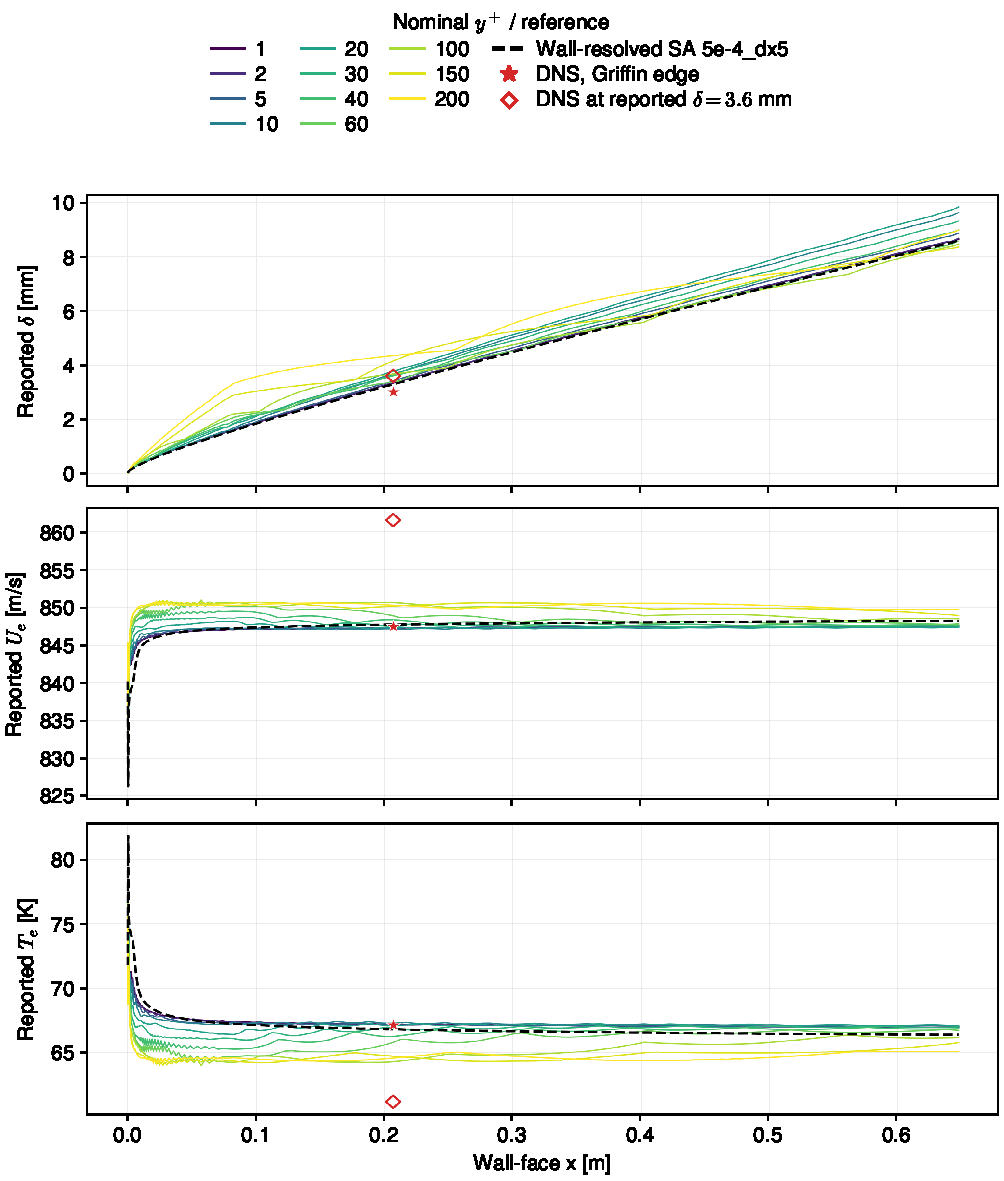
\includegraphics[width=\linewidth]{05_WF_Idea_Implementation/Griffin_Wallfunction_Edge_Quantities.pdf}
    \caption[Mesh sensitivity of the Griffin edge quantities]{Boundary layer thickness \(\delta\), edge velocity \(U_e\) and edge temperature \(T_e\) for M6Tw025. Colours identify conventional meshes by nominal first-cell \(y_1^+\); the dashed curve is the wall-resolved SA reference evaluated with the same criterion. Stars apply the Griffin criterion to the DNS profile, taking the unavailable mean wall-normal velocity as zero. Diamonds show the reported DNS thickness \(\delta=3.6\,\mathrm{mm}\) and the velocity and temperature interpolated at that height~\cite{zhang2018direct}.}
    \label{fig:wfs:BL_edge_quantities}
\end{figure}

\subsection{Application to RANS and limits of the published validation}
\label{subsec:wall-functions:griffin:validation-scope}

Griffin et al. describe the model as suitable for coupling to either LES or RANS. Their assessment combines a-priori tests on prescribed DNS profiles with a-posteriori WMLES of turbulent channels; it contains no coupled RANS validation~\cite[Sections~3--5]{griffin2023WF}. The principal comparisons use \(y_m=0.3\delta\), but the journal article also varies matching height during mesh refinement, including \(0.15\delta\) and \(0.075\delta\)~\cite[Section~4.1]{griffin2023WF}. These are matching locations, not prescribed first-cell-centre heights. As in WMLES it is common practice to retain off-wall resolutions below the point at which the wall model samples the boundary layer and then select the sample station adaptively dependant on the local boundary layer behaviour, i.e. if detachment is detected \cite{gao2026adaptive}. In addition to LES commonly using higher-order reconstruction methods, this may explain why Griffin et al. most likely didn't stumble upon  same mesh requirement issue (ref. Section \ref{subsec:comparative:zpg:yplus-sensitivity}).
\par\medskip

Here, the closure is coupled to SA through the near-wall turbulence constraint, with its wall shear and heat-flux delivered directly to HiSA as described in Section~\ref{subsec:wall-functions:direct-flux-delivery}. This RANS coupling and the reconstructed edge inputs require their own assessment. The published WMLES performance consequently provides no direct validation of the complete implementation. Nevertheless, the standalone closure can be checked against the published a-priori results, as shown in Table~\ref{tab:erriso:Griffin-a-priori-validation}. That consistency check supports the subsequent error-isolation study without implying equivalent accuracy of the coupled RANS calculations.

\section{Wang--Craft analytical wall function}
\label{sec:wall-functions:wang-craft}

The third an final wall function investigated in this work is by Wang et al \cite{wang2023WF}. It is unique compared Li et al and Griffin et al in that it does not rely on analytical momentum and energy closures, but rather on an analytical result of a proposed integral across the boundary layer. The downside of this approach being that it is not possible to run CFD independent analyses like the a-priori solves of the Li and Griffin wall functions (see Section~\ref{sec:comparative:zpg:cross-comparison}).
The implementation of this wall function raised several issue and ambiguities. Most notably on the streamwise integration necessary. While in the thesis work of Wang \cite{wang2019Thesis} it explicitly was implemented and tested on OpenFOAM there is no publicly available resource of the specific implementation. Contacting Wang unfortunately yielded in no response.
\par\medskip

The final implementation that was able to be achieved in the scope of this work showed some significant instabilities, most likely stemming from the downstream integration process at the leading edge of the flat-plates. Additionally the heat-flux and skin-friction output were unphysical. The afformentioned lack of a possibility to perform any kind of CFD-independent analysis further complicates debugging and identifying whether or not the issue is with the implementation or fundamentally with the wall function model - also because throughout the works of Wang on this wall function no investigation on a ZPG flat-plate was ever published. Thus it was decided to cut further debugging and development work in favour of spending the time on the analysis of the turbulence models and other two wall functions. 
\par\medskip

But for future research this wall function should anything but be disregarded, as it was the only investigated wall function that focused on, and proposed, good heat-flux and skin-friction prediction capability on SWBLI and complex geometries including separation.

\chapter{Benchmark cases and evaluation methodology}
\label{chap:evaluation-methodology}
Assessing wall-function performance requires consistent reference data, sufficiently resolved RANS baselines and explicit accuracy targets. This chapter introduces the selected zero-pressure-gradient (ZPG) flat-plate (FP) DNS benchmarks and their limitations, specifies the matching procedure and wall-resolved mesh requirements, and defines the criteria used to judge the results. These choices underpin the successive comparisons of turbulence modelling, wall-function closure and mesh sensitivity in Chapter~\ref{chap:comparative-evaluation}.

\section{Selected zero-pressure-gradient flat-plate DNS reference cases}
\label{sec:evaluation:benchmark-cases}

In this chapter the selected fully turbulent zero-pressure-gradient (ZPG) flat-plate (FP) cases used as references for the assessment of the aerothermal heating are being introduced as well as argued why they were chosen, or certain cases neglected. Furthermore in the respective subsections to each of the four primary sources of the DNS references, specific considerations that must be taken into account are highlighted.
\par\medskip

The four primary DNS references are from part 2 \cite{duan2010direct_part2} and part 4 \cite{duan2011direct_Part4} of Martin, Duan et al's four part series (further noted as "Martin-Duan Part 2" and "Martin-Duan Part 4" respectively) , Zhang et al \cite{zhang2018direct} and Huang et al \cite{huang2020simulation}. The selected benchmarks comprise 12 distinct ZPG flat-plate cases, summarized in Table \ref{tab:evaluation:selected-cases}.
\begin{table}[H]
    \centering
    \caption{Selected ZPG flat-plate DNS benchmark cases.}
    \label{tab:evaluation:selected-cases}
    \begin{tabular}{@{}lp{0.62\linewidth}@{}}
        \toprule
        DNS reference & Selected cases \\
        \midrule
        Martin-Duan Part 2 &
        M5T1, M5T2, M5T3, M5T4, M5T5 (adiabatic) \\
        \addlinespace
        Martin-Duan Part 4 &
        LowH\_M3 \\
        \addlinespace
        Zhang &
        M2p5 (adiabatic), M6Tw025, M6Tw076*,
        M8Tw048, M14Tw018 \\
        \addlinespace
        Huang &
        M11Tw020 (stations BL1, BL2, and BL3) \\
        \bottomrule
    \end{tabular}
\end{table}

Case names are retained from the respective publications. The number after \(M\) indicates the nominal freestream Mach number, \(T\) distinguishes the wall-temperature variants in Martin--Duan Part~2. Their thermal conditions are taken from the reported data rather than inferred from the case names. For Zhang and Huang, \(Tw\) denotes the wall-to-recovery temperature ratio \(T_w/T_r\), with recovery factor \(r=0.89\)~\cite[Nomenclature]{zhang2018direct}. Huang's M11Tw020 case is sampled at three downstream stations, BL1--BL3. The asterisk marks the M6Tw076 temperature note below.
\par\medskip

These cases were selected as suitable references because they span a wide range of super- to hypersonic cold-wall regime as well as varying degrees of compressibility as indicated in Figure~\ref{fig:evaluation:dns-bq-mtau} range on the heat-transfer coefficient \(-B_q\) and friction Mach number \(M_\tau\) respectively. \(M_\tau\) is discussed by Smits and Dussauge~\cite{smits2006turbulent} and used here as an indicator for intrinsic compressibility effects, following Hasan et al.~\cite{hasan2025intrinsic}. With cold-wall and compressibility effects seemingly being the dominant factors differentiating hypersonic cold-wall boundary layers from incompressible ones, it was chosen to plot Figure~\ref{fig:evaluation:dns-bq-mtau} using \(-B_q\) and \(M_\tau\). The selected DNS cases don't span the whole  \(-B_q\)-\(M_\tau\) domain and mainly lie clustered on a line. This could partly be attributed to the fact that the friction velocity \(u_\tau\) is scaling both axes, or it may represent a genuine gap in DNS references which may yield interesting insights. To fully judge and address the real-world extend findings based on these DNS references can be applied, further variables such as a Reynolds number might add important value too, so as not to extrapolate findings of this work into non-applicable domains.
\par\medskip

For the cases by Zhang et al it should be positively highlighted that the data has been additionally published digitally at \url{https://tmbwg.github.io/turbmodels/Other_DNS_Data/supersonic_hypersonic_flatplate.html} [accessed 14 September 2026], although the first reported off-wall data point is already at a y\(^+ = 0.5\).

\begin{figure}[H]
    \centering
    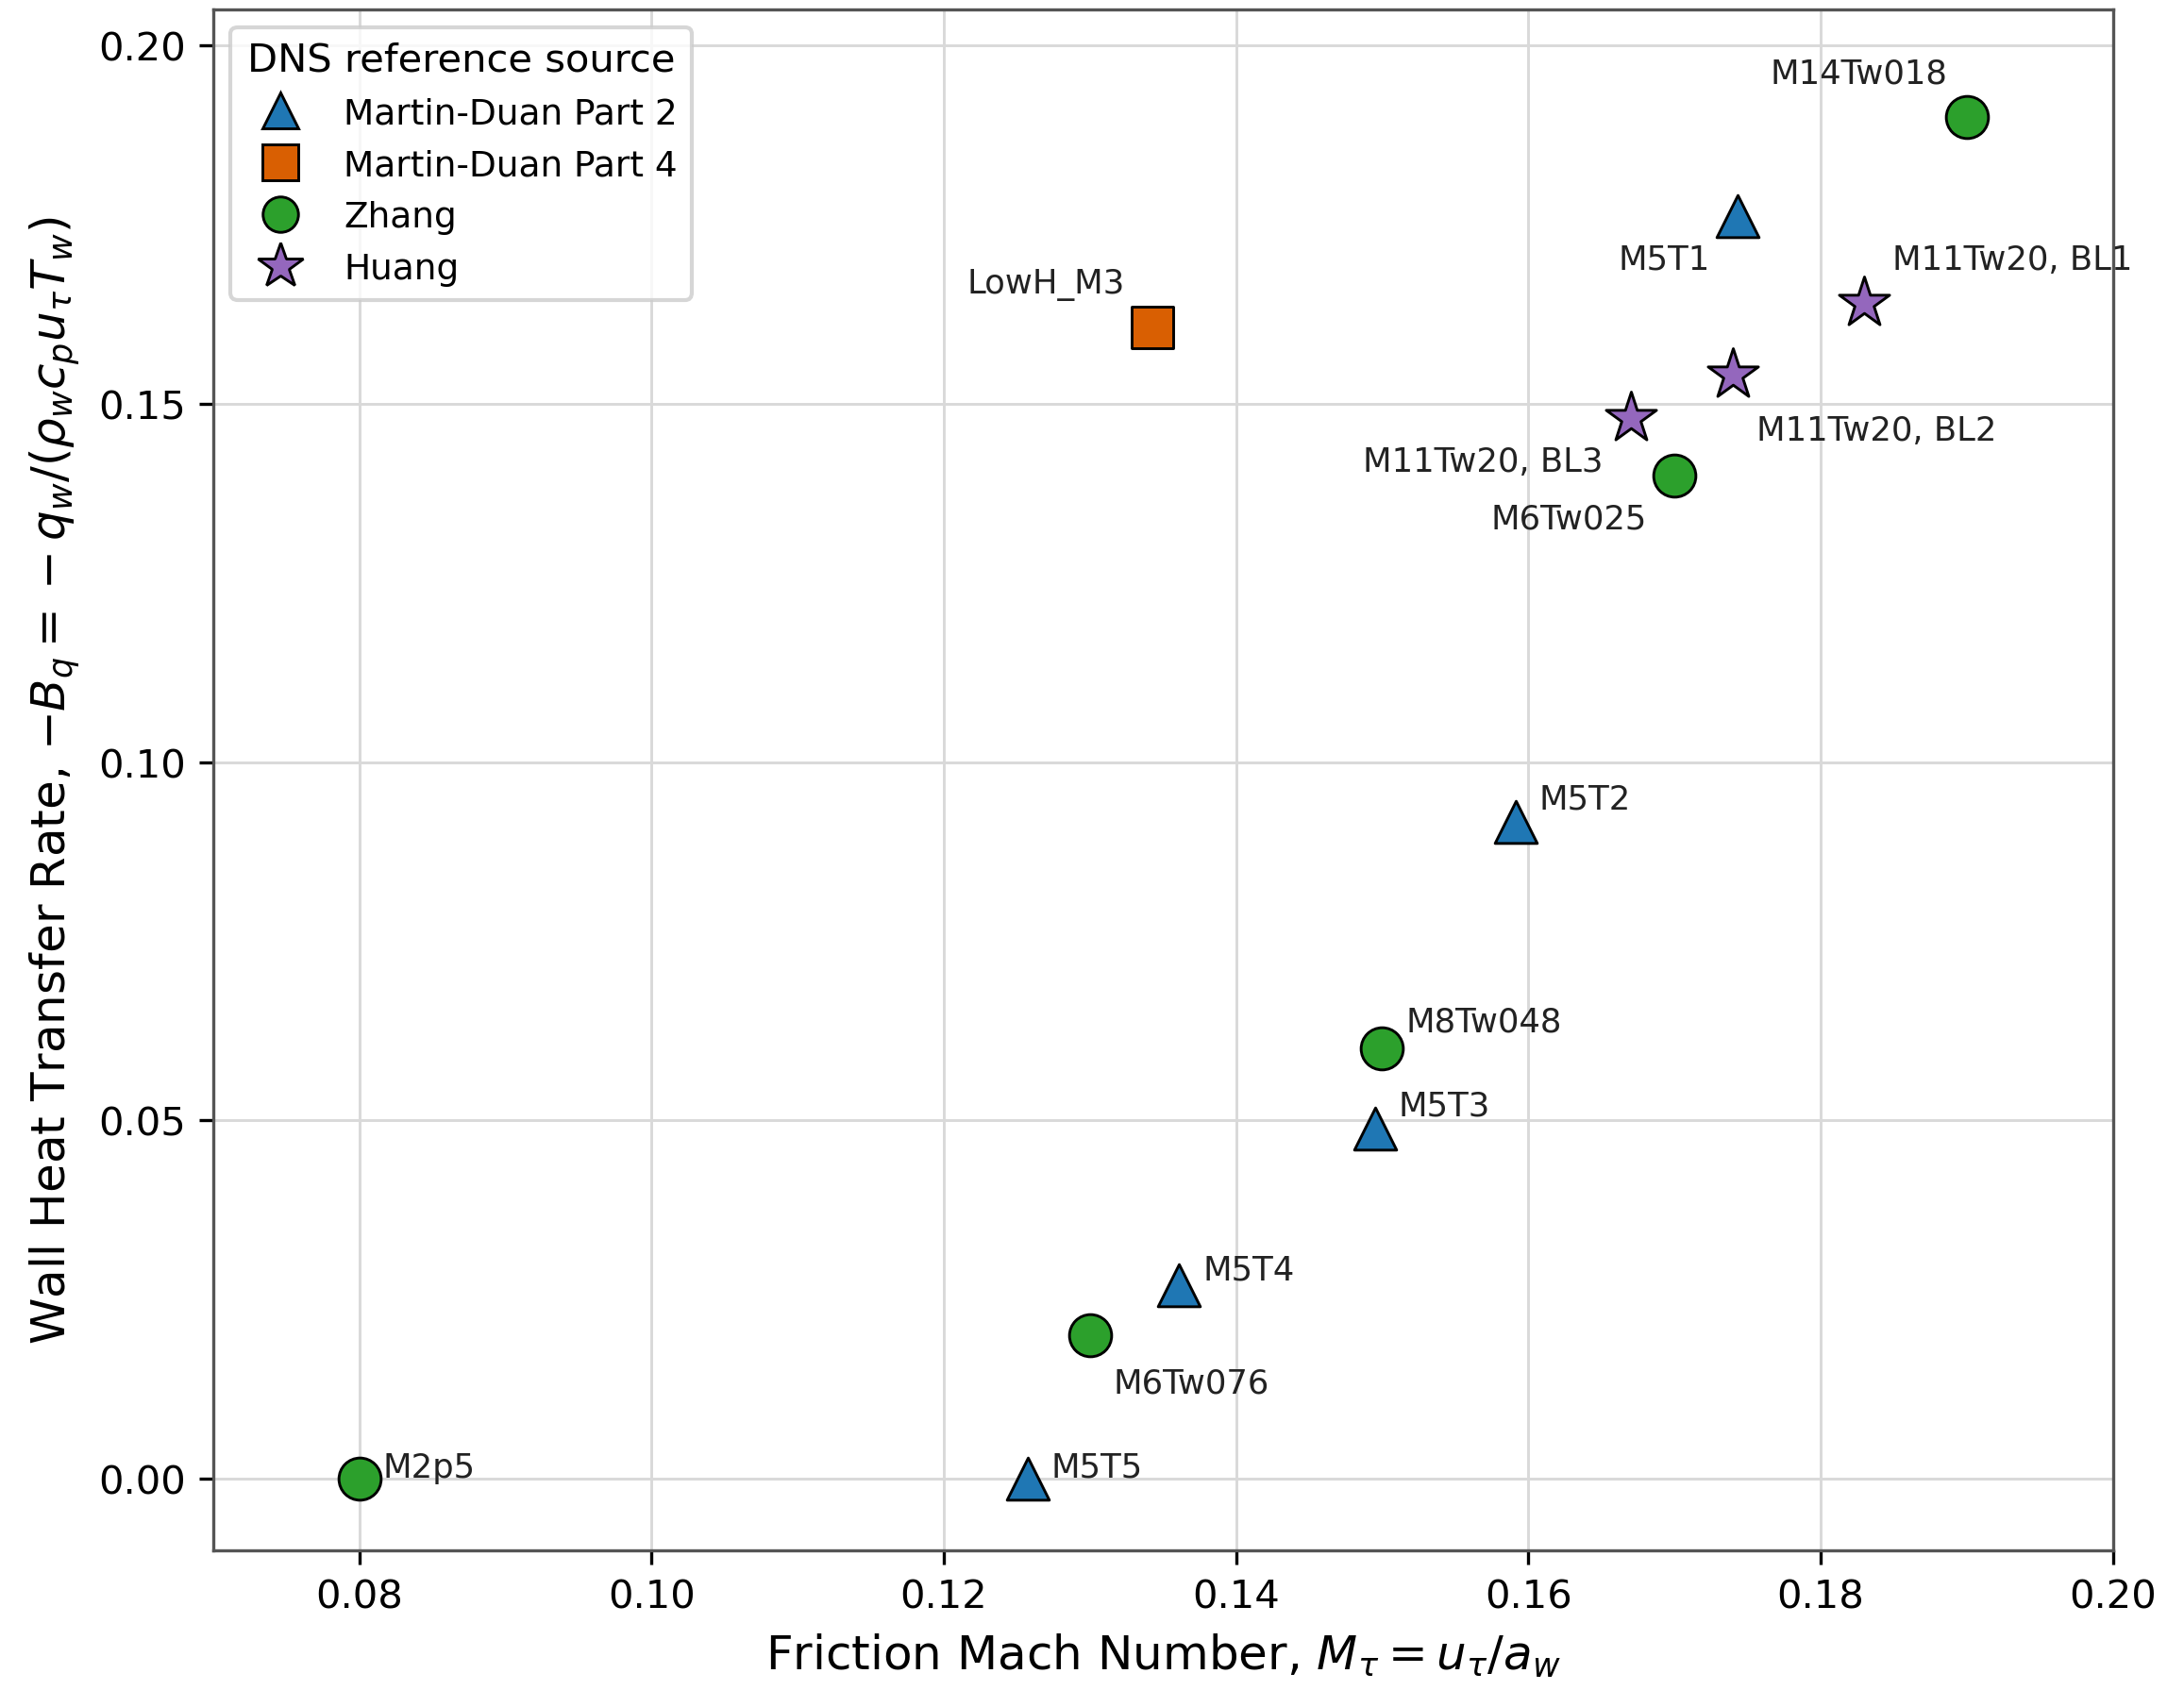
\includegraphics[width=\linewidth]{06_Eval_Methodology/06_Figures/DNS_minus_Bq_vs_M_tau (2).png}
    \caption{Selected DNS benchmark cases in terms of the dimensionless wall heat-transfer rate \(-B_q\) and friction Mach number \(M_\tau\).}
    \label{fig:evaluation:dns-bq-mtau}
\end{figure}

To put the cold-wall strengths of the twelve investigated ZPG flat-plates into perspective of real world flight conditions, the fraction \(\frac{T_w}{T_{r}}\) of the DLR's flight experiment STORT is looked at, where \(T_r\) is the adiabatic recovery temperature. The heat-transfer rate \(-B_q\) is arguably a more comparable assessment of the cold-wall effects, but with flight experiments the skin-friction is rarely if ever available. For the calculation of the \(\frac{T_w}{T_r}\) during the STORT flight, the published thermo couple readings of the surface temperature on the nose cone at 40, 152.1 and 150.5 mm from the nose tip \cite[Figure 10]{reimer2025stort} and the flight Mach numbers \cite[Figure 9 (b)]{reimer2025stort} are used. For simplification, and as this shall only serve as a rough estimation and insight to real world flight, perfect gas with \(\gamma = 1.4\) and a recovery factor of \(r = 0.89\) is assumed. Furthermore the calculations are simplified in assuming the freestream conditions as the boundary layer edge quantities, which is fine for ZPG flat-plates, but with the temperature probes sitting on the nosecone and somewhat close to the nose's bow shock it is arguably a rough engineering approximation, but measurements or high fidelity simulation results of the actual temperature boundary layer are not available. Thus figure should be understood as an indicative plot and not as an exact categorization of the cold-wall strength the STORT flight experienced. Never the less Figure \ref{fig:evaluation:stort-Twall-Tad} shows that \(\frac{T_w}{T_r}\) ratios of e.g. 0.25, like herein investigated in the M6Tw025 ZPG flat-plate, are not extraordinarily cold-walls, and well within what a hypersonic vehicle can experience. But when looking at validation of RANS models, adiabatic or even slightly warm walls (i.e. negative heat-flux, from the wall to the fluid) are to be looked at, but then again it all is very case-by-case dependant on the material, or trajectory.

\begin{figure}[H]
    \centering
    % Notation-only regeneration (2026-10-19): T_ad -> T_r in display labels.
    % Source: /home/mgnadlinger/ZPG_FP_overview/STORT/recovery_temperature/plot_stort_recovery.py
    % Data: /home/mgnadlinger/ZPG_FP_overview/STORT/STORT_experiment_data.xlsx
    % Wrapper/audit: tmp/notation_figures_20261019/regenerate_stort.py and stort_audit.json.
    % Prior notation-only pass retained the original manuscript crop and image dimensions.
    % Caption-sized font regeneration (2026-10-19): 10 pt at 170 mm manuscript width.
    % Reproducible script: 06_Figures/plot_stort_caption_fonts.py; archived original
    % script/workbook and numerical/layout audit: 06_Figures/stort_sources/.
    % All plotted samples, axes limits and the calculation CSV are unchanged.
    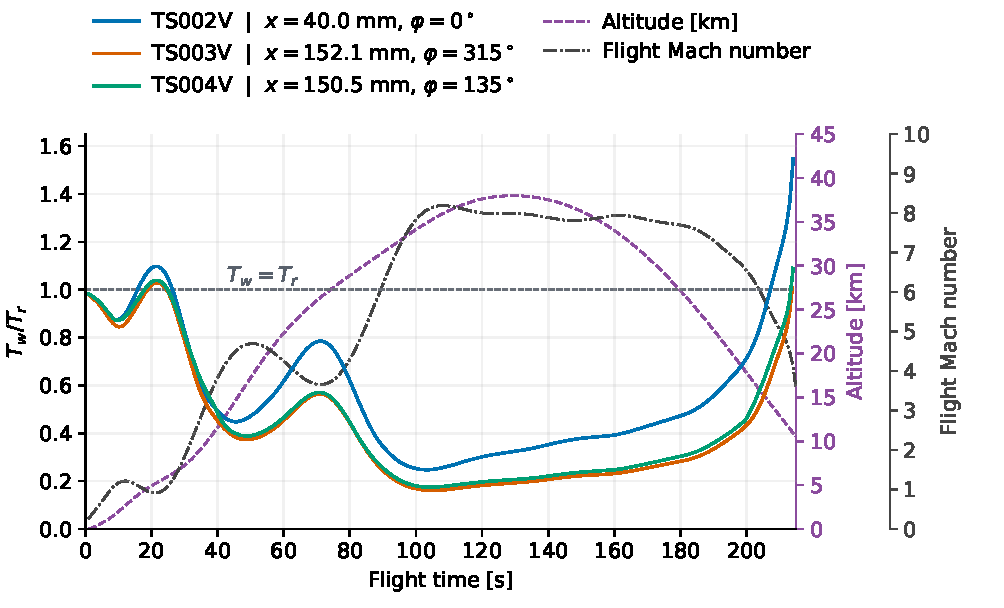
\includegraphics[width=\linewidth]{06_Eval_Methodology/06_Figures/STORT_Twall_Tad.pdf}
    \caption{Indicative \(T_w/T_r\) ratio experienced by the DLR's STORT hypersonic flight experiment \cite{gulhan2022objectives}. TS002V, TS003V and TS004V are the surface thermal couples as reported in \cite{reimer2025stort}, with their location on the nose cone, as measured in millimetres from the nose tip.}
    \label{fig:evaluation:stort-Twall-Tad}
\end{figure}

\subsection{Inflow and wall conditions}

In this section the inflow and wall conditions of the reference DNS cases are extracted from the respective sources and discussed. For this work it was elected to assign the reported freestream conditions, as reported in the tables below, at the inlet in a uniform manner. In \ref{subsec:comparative:zpg:results-assessment} a publication by Vaughen argued for using back calculated pre-shock conditions instead - a sensitivity analysis was performed and revealed limited affect and no clear claim of which approach, DNS freestream or back calculated pre-shock values are a more correct replication of the DNS cases. 

\paragraph*{Martin-Duan}

Martin-Duan Part 2 and Martin-Duan Part 4 are both created using an initial RANS simulation with added transformed DNS fluctuations followed by a recycling scheme to develop the boundary layer along the flat-plate temporally with streamwise periodic boundary conditions \cite{martin2007direct_Part1}. The inflow conditions selected are taken from the reported freestream conditions for the Mach 5 case in Table 1 of \cite{martin2007direct_Part1}, which are reiterated or derived from it here in Table \ref{tab:evaluation:martin-duan-inflow-wall}, similarly for the LowH\_M3 case the freestream conditions are defined in \cite[Table 1]{duan2011direct_Part4}. The only difference in the M5T1 to M5T5 cases are the isothermal wall temperature.
\par\medskip

Martin-Duan Part 4 contains additional reacting references cases, which are beyond the scope of this work, and additionally a calorically and thermally perfect case, named LowH\_M10. This case is intentionally omitted because of it represents an incredibly far downstream station as a result of multiple recycling which leads to an over 1.3 metre thick boundary layer at the matching station \cite[Table 2]{duan2011direct_Part4}. This is also highlighted by the authors themselves, and noted that “the flow conditions themselves might not be realistic” \cite{duan2011direct_Part4}.

\begin{table}[H]
    \centering
    \caption{Freestream inflow and wall conditions for the Martin-Duan cases.}
    \label{tab:evaluation:martin-duan-inflow-wall}
    \begin{tabular}{l S[table-format=1.2] S[table-format=1.4] S[table-format=3.2] S[table-format=4.2]}
        \toprule
        Case & {\(M_\infty\)} & {\(\rho_\infty\;[\mathrm{kg}/\mathrm{m}^3]\)} & {\(T_\infty\;[\mathrm{K}]\)} & {\(T_w\;[\mathrm{K}]\)} \\
        \midrule
        M5T1 & 5.00 & 0.0889 & 216.65 & 228.1 \\
        M5T2 & 5.00 & 0.0889 & 216.65 & 433.30 \\
        M5T3 & 5.00 & 0.0889 & 216.65 & 649.95 \\
        M5T4 & 5.00 & 0.0889 & 216.65 & 866.60 \\
        M5T5 & 5.00 & 0.0889 & 216.65 & 1191.6 \\
        LowH\_M3 & 3.5 & 0.0184 & 226.5 & 125 \\
        \bottomrule
    \end{tabular}
\end{table}

For M5T1, the prescribed wall temperature \(T_w=228.1\,\mathrm{K}\) follows Part~2 Table~1, which gives \(T_w/T_\delta=1.00\) and \(T_\delta=228.1\,\mathrm{K}\)~\cite{duan2010direct_part2}. The separate Reynolds-number inconsistency is examined in Appendix~\ref{app:duan-part2-consistency}.

\paragraph*{Zhang}

Zhang et al.’s DNS database comprises spatially developing flat-plate turbulent boundary layers with turbulent inflow supplied by a modified recycling/rescaling method. An extended downstream development region allows artificial effects of inflow generation to decay before statistics are evaluated \cite{zhang2018direct}. The cases were selected in a way to represent various experimental hypersonic wind tunnel experimental conditions. The freestream inflow quantities are taken from \cite[Tbale 1]{zhang2018direct} and reiterated here in Table \ref{tab:evaluation:zhang-inflow-wall}.

\begin{table}[H]
    \centering
    \caption{Freestream inflow and wall conditions for the Zhang cases.}
    \label{tab:evaluation:zhang-inflow-wall}
    \begin{tabular}{l S[table-format=2.2] S[table-format=1.3] S[table-format=3.1] S[table-format=3.1,table-space-text-post={*},table-align-text-after=false]}
        \toprule
        Case & {\(M_\infty\)} & {\(\rho_\infty\;[\mathrm{kg}/\mathrm{m}^3]\)} & {\(T_\infty\;[\mathrm{K}]\)} & {\(T_w\;[\mathrm{K}]\)} \\
        \midrule
        M2P5 & 2.50 & 0.100 & 270.0 & {(adiabatic)} \\
        M6Tw025 & 5.84 & 0.044 & 55.2 & 97.5 \\
        M6Tw076 & 5.86 & 0.043 & 55.0 & 300.0{*} \\
        M8Tw048 & 7.87 & 0.026 & 51.8 & 298.0 \\
        M14Tw018 & 13.64 & 0.017 & 47.4 & 300.0 \\
        \bottomrule
    \end{tabular}
\end{table}

The asterisk ``*'' on the M6Tw076 case's \(T_w\) comes from an inconsistency between the paper's Table 1 reported \(T_w = 300 K\) and the digitally published boundary profile data which at the wall face (\(z = 0\)), reports a \(T/T_\infty = 5.38\), which, with the paper's Table 1 reported \(T_\infty = 55.0 \mathrm{K}\), results in a \(T_w = 295.9 \mathrm{K}\). This \(4 \mathrm{K}\) is a minor inconsistency, but in some Temperature related plots is a visible. Furthermore, with the M6Tw076 being almost adiabatic with a reported \(-B_q = 0.02\) \cite[Table 2]{zhang2018direct}, this wall temperature deviation can carry a higher than expected uncertainty for the wall heat-flux.

\paragraph*{Huang}

Huang et al use a precursor RANS simulation similar to Duan and Martin, with turbulent inflow generated by recycling/rescaling and subsequently spatially developing boundary layer through three overlapping DNS boxes. The freestream and isothermal wall-temperature conditions are taken from the reported Table 1 in \cite{huang2020simulation}.

\begin{table}[H]
    \centering
    \caption{Freestream inflow and wall conditions for the Huang case.}
    \label{tab:evaluation:huang-inflow-wall}
    \begin{tabular}{l S[table-format=2.1] S[table-format=1.3] S[table-format=2.1] S[table-format=3.0]}
        \toprule
        Case & {\(M_\infty\)} & {\(\rho_\infty\;[\mathrm{kg}/\mathrm{m}^3]\)} & {\(T_\infty\;[\mathrm{K}]\)} & {\(T_w\;[\mathrm{K}]\)} \\
        \midrule
        M11Tw020 & 10.9 & 0.103 & 66.5 & 300 \\
        \bottomrule
    \end{tabular}
\end{table}

\subsection{Thermal and transport models}

All of the investigated DNS references herein represent thermally and calorically perfect gases. With the exception of the M8Tw048 case, which represent pure Nitrogen, all of the DNS references represent air.

\begin{table}[H]
    \centering
    \caption{Thermal models defined in or reasonably inferrable from the DNS references.}
    \label{tab:evaluation:thermal-models}
    \begin{tabular}{l S[table-format=4.2,table-space-text-post={*},table-align-text-after=false] S[table-format=1.1,table-space-text-post={*},table-align-text-after=false] S[table-format=3.2,table-space-text-post={*},table-align-text-after=false] S[table-format=1.2]}
        \toprule
        Case & {\(c_{p,\infty}\;[\mathrm{J}/\mathrm{kg\,K}]\)} & {\(\gamma_\infty\)} & {\(R\;[\mathrm{J}/\mathrm{kg\,K}]\)} & {\(Pr\)} \\
        \midrule
        Martin-Duan Part 2/4 & 1004.5 & 1.4 & 287 & {(not defined)} \\
        Zhang & 1004.5 & 1.4 & 287 & 0.71 \\
        Zhang - M8Tw048 & 1039.68{*} & 1.4{*} & 297.05{*} & 0.71 \\
        Huang & 1004.5 & 1.4 & 287 & 0.71 \\
        \bottomrule
    \end{tabular}
\end{table}

The Martin-Duan cases leave the most ambiguity, as throughout their four part series they only ever state "the working fluid is air" \cite[p. 422]{duan2010direct_part2}. For the molecular Prandtl number, Martin and Duan give no explicit value or a law for the conductivity law to infer it. It was chosen to go with a \(Pr = 0.71\) as the other references also do so and it is a common value to use for perfect air.
\par\medskip

The asterisk ``*'' on the M8Tw048 case is because it suffers similar ambiguity, where the \(\gamma\), \(R\) or \(c_p\) are not defined, rather the \(\gamma \) must be derived through the given recovery temperature ratio. Subsequently, through \(\frac{M}{U_\infty} = \sqrt{\gamma R T}\) and \(c_p = \frac{\gamma R}{\gamma - 1}\), the thermal gas model can be fully inferred, with the specific gas constant for diatomic Nitrogen given as \(R = 296.803 \mathrm{J}/\mathrm{kg\,K}\) by NIST\footnote{[accessed 14 September 2026] \url{https://webbook.nist.gov/cgi/cbook.cgi?ID=7727-37-9}}.


\begin{table}[H]
    \centering
    \caption{Viscosity laws defined in or reasonably inferrable from the DNS references.}
    \label{tab:evaluation:viscosity-laws}
    \centering
    \renewcommand{\arraystretch}{1.5}
    \begin{tabular}{@{}lll@{}}
        \toprule
        Case & Model & Dynamic viscosity \(\mu(T)\) \\
        \midrule
        Martin-Duan Part 2/4 & Power law\textsuperscript{*} & \(\displaystyle \mu_\delta\left(\frac{T}{T_\delta}\right)^{0.76}\) \\
        \addlinespace[1ex]
        Zhang & Sutherland & \(\displaystyle 1.458\times10^{-6}\,\frac{T^{3/2}}{T+110.4}\) \\
        \addlinespace[1ex]
        Zhang - M8Tw048 & Keyes & \(\displaystyle 1.418\times10^{-6}\,\frac{T^{3/2}}{T+116.4\times10^{-5/T}}\)\footnotemark \\
        \addlinespace[1ex]
        Huang & Sutherland & \(\displaystyle 1.458\times10^{-6}\,\frac{T^{3/2}}{T+110.4}\) \\
        \addlinespace[0.5ex]
        \bottomrule
    \end{tabular}
\end{table}
\footnotetext{As stated in digitally published \texttt{M8Tw048\_Stat.dat} file.}

The asterisk ``*'' on Martin-Duan is because in their initial case description they do not state more than just "is the temperature dependent viscosity and is computed using a power law" \cite[p. 348]{martin2007direct_Part1}, in Part 4 then explicitly stated as power law with exponent \(0.76\) and using edge viscosity and Temperature as reference - with \(\mu_\delta\) calculated from Sutherland if \(T_\delta \geq 170 \mathrm{K}\), otherwise Keyes model \cite[Eq. 2.14 and following text]{duan2011direct_Part4} - all Martin-Duan cases are modelled after this concept, as it is reasonable to assume that throughout the four part series this wasn't changed.

\paragraph*{Implementation of viscosity law and constant molecular Prandtl number}
The registered thermophysical combinations described in
Section~\ref{subsec:ext:thermo-physical-extension} permit the reference
viscosity laws in Table~\ref{tab:evaluation:viscosity-laws} to be represented
by seventh-order polynomials with independently specified conductivity.
For the constant-\(c_p\) benchmarks, setting the conductivity coefficients to
\(c_p/Pr\) times the viscosity coefficients enforces the selected constant
molecular Prandtl number. This reproduces the required combination of
viscosity and conductivity laws without adopting the conductivity relation
of the standard \texttt{sutherland} transport model.
\par\medskip

Over the minimum and maximum temperature range reported by the solver, the fitted viscosity polynomials were a-priori evaluated against the stated laws, with the assessment present in every case's \texttt{/constant/}-folder, like e.g. in figure \ref{fig:evaluation:viscosity-fit} for the M6Tw025 case. 
\begin{figure}[H]
    \centering
    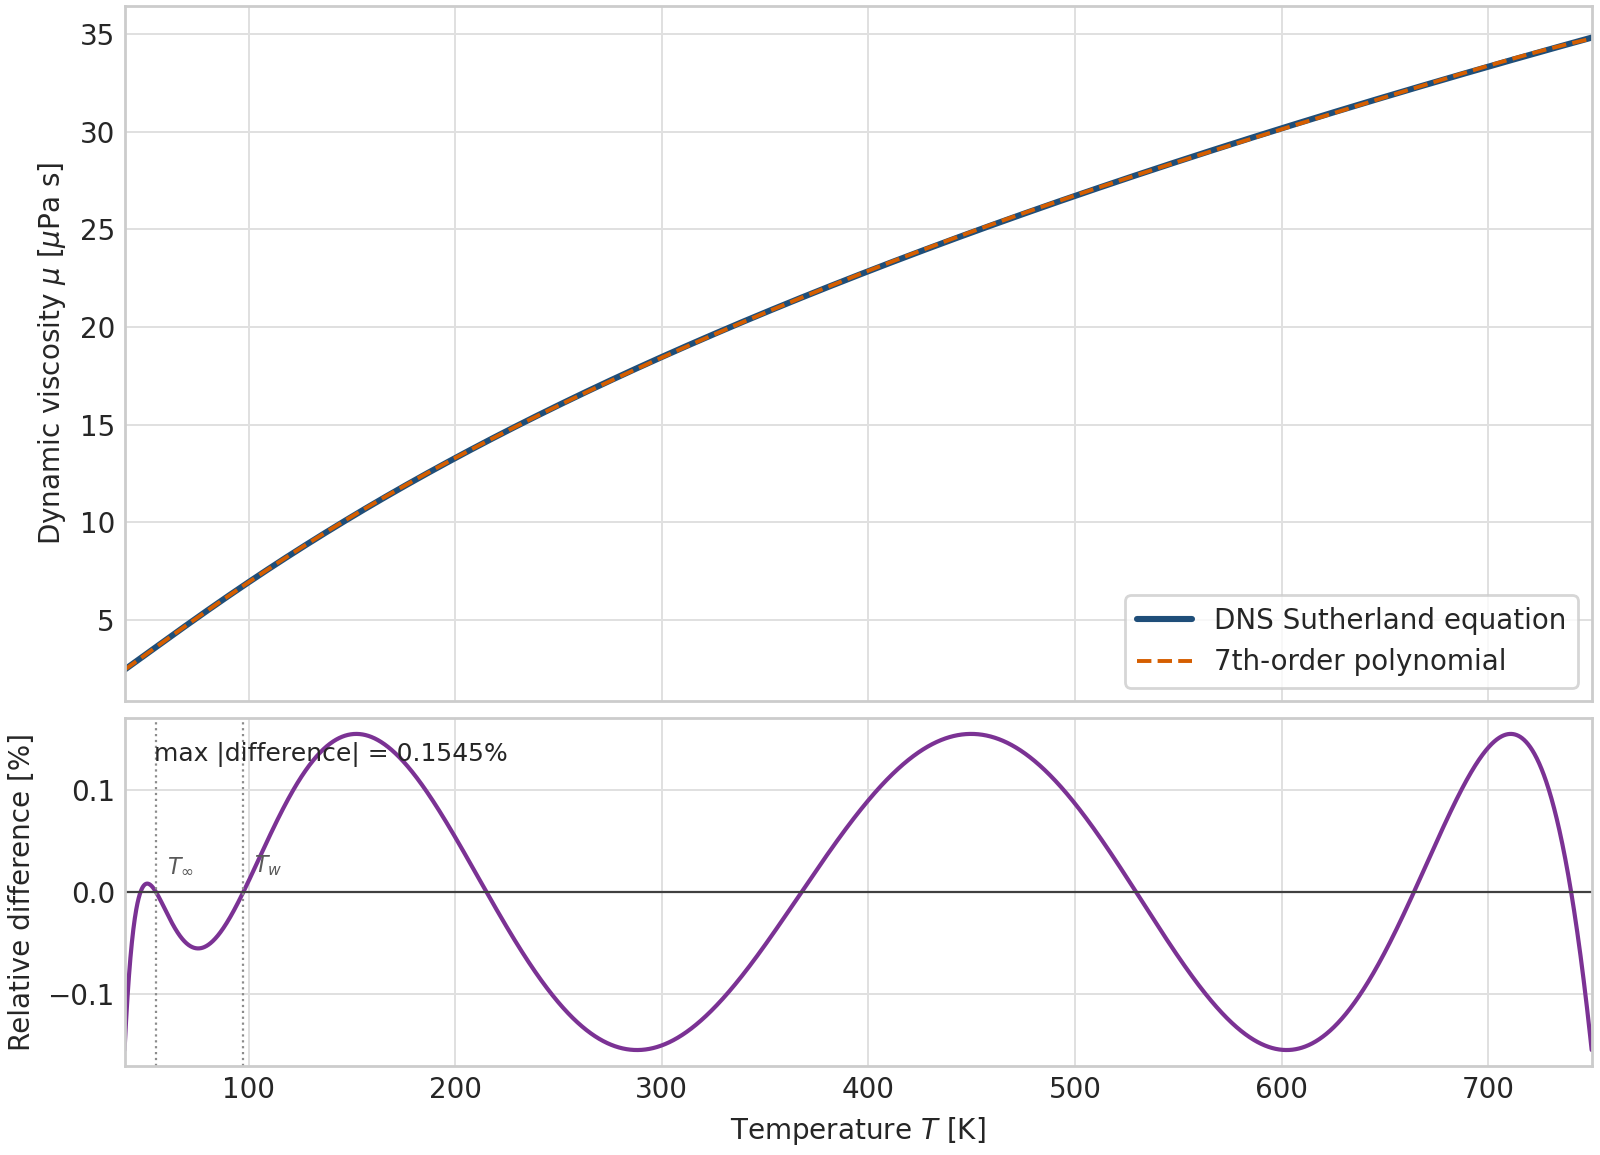
\includegraphics[width=0.8\linewidth]{06_Eval_Methodology/06_Figures/M6Tw025_sutherland_polynomial_fit.png}
    \caption{Assessment of the custom 7th-order polynomial fit for the dynamic viscosity on the M6Tw025 case, against the DNS reference's defined viscosity law. With fixed points at the \(T_w\) and \(T_\infty\).}
    \label{fig:evaluation:viscosity-fit}
\end{figure}

\paragraph*{Turbulent Prandtl number}
\label{para:turbulent-Prandtl-number}

Unless explicitly stated otherwise, the SA and \(k\)--\(\omega\) SST simulations use a constant turbulent Prandtl number \(Pr_t=0.9\). This follows common RANS practice beyond OpenFOAM: the NATO AVT-352 cone--flare comparison reports constant values of \(0.9\) for DLR TAU and NASA VULCAN, \(0.89\) for STAR-CCM+, and \(0.85\) for the Aselsan Ansys Fluent calculations~\cite[Section~IV]{hoste2025review}. NASA's LAURA manual likewise specifies \(Pr_t=0.9\) as the default~\cite[Section~5.4.17]{Thompson2024LAURA}. The present choice therefore provides a conventional baseline, retained across the benchmark set to compare the models under a common thermal-closure assumption and it is not fitted separately to each DNS case. DNS turbulent-Prandtl-number distributions and a sensitivity calculation with other constant values are discussed with the wall-resolved profile results in Section~\ref{subsec:comparative:zpg:wr-prandtl}.

\subsection{Matching station, quantities and figures of interest}
\label{subsec:evaluation:matching-station}
% Writing prerequisite for Chapter 7: keep the source-specific Re_delta2
% definitions, DNS-to-WR matching and common physical station for WF-to-WR
% comparisons explicit. Distinguish these from the Re_tau-based Pr_t sensitivity
% comparison, and distinguish q_w/tau_w from coefficients with different edge
% or freestream normalizations.


\paragraph*{On the definition of the matching station between RANS result and DNS reference}

The 12 DNS references only provide information about the boundary layer profile and the wall heat-flux and shear stress at a singular downstream station - the Huang case being the exception with providing three downstream stations. Still some studies using the same ZPG FPs, e.g. \cite{huang2019assessment}, \cite{xue2024assessment}, or \cite{aiken2022assessment} plot multiple downstream stations, although it is not traceable from these publications where exactly they got these values from. For the later sections, it is thus abstained form including them, and it is strictly adhered to comparing to the primary source's values. Still plotting the downstream development of the quantities is crucial to judging their development rather than just one snapshot. This is will become apparent on some later figures like Figure~\ref{fig:evaluation:SA-mesh-convergence-behaviour}.
\par\medskip

Another crucial point to assess, is at what spatial location to compare the RANS results with the DNS reference. This matching point can be determined by e.g. matching a physical downstream x-station, Reynolds number based on shear velocity \(Re_\tau\), Reynolds number based on momentum thickness and wall viscosity \(Re_{\delta2}\), or Reynolds number based on momentum thickness and freestream viscosity \(Re_\theta\).
\par\medskip

Matching on a physical downstream x-station is not possible because the DNS references do not provide this information with regards to the actual beginning of the boundary layer development. As the ZPG DNS cases investigated in here represent fully turbulent boundary layers and no natural or forced tripping, they are set up with predetermined turbulent boundary layers at the inlet. They subsequently report the boundary layer thickness assigned at the inlet as \(\delta_i\), and either the physical downstream sample station in the DNS domain, \(x_a\), or the ratio \(\frac{x_a}{\delta_i}\).Neither \(x_a\) or it's non-dimensionless ratio with \(delta_i\) sufficiently defines the physical downstream station in a RANS domain where the boundary layer is being developed from the leading edge onwards. Also the inlet profiles used for the DNS' are not available to exactly reproduce the domain from the same starting point.
\par\medskip

Just five weeks before hand-in of this work, Cheng et al in \cite{cheng2026reynolds} investigated the same Zhang and Huang ZPG flat-plates on RANS energy closure (see previous paragraph~\ref{para:turbulent-Prandtl-number}). Cheng et al used a novel matching station approach for their work, where they first determined the physical streamwise station at which the RANS solution produces the same boundary layer thickness as reported inflow boundary layer thickness \(\delta_i\) in the DNS references. Subsequently the DNS matched sample station is then determined by the DNS reported ratio \(\frac{x_a}{\delta_i}\), where \(x_a\) the physical downstream location in the DNS domain, from this matched boundary layer thickness \(\delta_i\). Tables~\ref{tab:evaluation:matching-station-bq} and ~\ref{tab:evaluation:matching-station-ch} however shows that the \(Re_{\delta2}\) matching chosen for this work, and a physical boundary layer distance shifted matching like done by Cheng et al., agree within 1\% for \(-B_q\) and less than 2\% for \(C_h\). 

\begin{table}[H]
    \centering
    \caption{Comparison of the dimensionless wall heat-transfer rate \(-B_q\) from DNS (D), RANS at the shifted physical matching station as proposed by Cheng et al. (S), and RANS at the \(Re_{\delta2}\)-matched station (R). Relative differences are given in percent.  The RANS solutions are from the wall-resolved \(k\)--\(\omega\) SST simulations as introduced later in Section~\ref{subsec:comparative:zpg:wr-wall-fluxes}.}
    \label{tab:evaluation:matching-station-bq}
    \small
    \setlength{\tabcolsep}{4pt}
    \begin{tabular}{@{}l S[table-format=1.2] S[table-format=1.9] S[table-format=1.9] S[table-format=-2.2] S[table-format=-2.2] S[table-format=+1.2]@{}}
        \toprule
        Case & {\shortstack{DNS (D)\\\(-B_q\)}} & {\shortstack{Shifted (S)\\\(-B_q\)}} & {\shortstack{\(Re_{\delta2}\) (R)\\\(-B_q\)}} & {\shortstack{S vs D\\{[\%]}}} & {\shortstack{R vs D\\{[\%]}}} & {\shortstack{S vs R\\{[\%]}}} \\
        \midrule
        M6Tw025  & 0.14 & 0.138455697 & 0.137434751 & -1.10  & -1.83  & +0.74 \\
        M6Tw076  & 0.02 & 0.017508213 & 0.017582069 & -12.46 & -12.09 & -0.42 \\
        M8Tw048  & 0.06 & 0.058947522 & 0.058587750 & -1.75  & -2.35  & +0.61 \\
        M14Tw018 & 0.19 & 0.186542796 & 0.185085083 & -1.82  & -2.59  & +0.79 \\
        \bottomrule
    \end{tabular}
\end{table}

\begin{table}[H]
    \centering
    \caption{Comparison of the Stanton number \(C_h\) from DNS (D), RANS at the shifted physical matching station as proposed by Cheng et al. (S), and RANS at the \(Re_{\delta2}\)-matched station (R). Relative differences are given in percent. The RANS solutions are from the wall-resolved \(k\)--\(\omega\) SST simulations as introduced later in Section~\ref{subsec:comparative:zpg:wr-wall-fluxes}.}
    \label{tab:evaluation:matching-station-ch}
    \small
    \setlength{\tabcolsep}{4pt}
    \begin{tabular}{@{}l S[table-format=1.9] S[table-format=1.9] S[table-format=1.9] S[table-format=+2.2] S[table-format=+2.2] S[table-format=+1.2]@{}}
        \toprule
        Case & {\shortstack{DNS (D)\\\(C_h\)}} & {\shortstack{Shifted (S)\\\(C_h\)}} & {\shortstack{\(Re_{\delta2}\) (R)\\\(C_h\)}} & {\shortstack{S vs D\\{[\%]}}} & {\shortstack{R vs D\\{[\%]}}} & {\shortstack{S vs R\\{[\%]}}} \\
        \midrule
        M6Tw025  & 0.001021456 & 0.001067416 & 0.001050667 & +4.50  & +2.86  & +1.59 \\
        M6Tw076  & 0.000633588 & 0.000546307 & 0.000551478 & -13.78 & -12.96 & -0.94 \\
        M8Tw048  & 0.000448561 & 0.000462389 & 0.000456311 & +3.08  & +1.73  & +1.33 \\
        M14Tw018 & 0.000243366 & 0.000282753 & 0.000277646 & +16.18 & +14.09 & +1.84 \\
        \bottomrule
    \end{tabular}
\end{table}

\begin{equation}
    Re_\tau = \frac{\rho_w u_\tau \delta}{\mu_w}
\end{equation}
Matching on the \(Re_\tau\) is seen rather often, e.g. \cite{xue2024assessment}, or \cite{aiken2022assessment}. It has the advantage that by definition of \(Re_\tau\) being calculated with the boundary layer thickness \(\delta\), this matching ensure equally thick developed boundary layer. The drawback however is that \(Re_\tau\), also relies on the shear velocity \(u_\tau\), thus any matching with \(Re_\tau\) is also an indirect matching on the skin-friction, which undermines subsequent findings on the wall shear stress behaviour. A potential ambiguity in the definition of \(Re_\tau\), is the definition of the boundary layer thickness. Whereas most often the boundary layer thickness is defined as the wall-normal distance where \(U = 99\% U_\infty\), often noted as \(\delta_{99}\), as discussed in Griffin Section~\ref{subsec:wall-functions:griffin:edge-detection}, this doesn't necessary always have to be the case, or e.g. in Huang's reference where it is rather defined as "99.5\% of the freestream total enthalpy" \cite[Nomenclature]{huang2020simulation}.

\begin{equation}
    Re_\theta = \frac{\rho_\infty u_\infty \theta}{\mu_\infty}, \qquad \text{or} \qquad Re_{\delta2} = \frac{\rho_\infty u_\infty \theta}{\mu_w},
\end{equation}
with
\begin{equation}
    \theta = \int_0^\delta \frac{\rho u}{\rho_e u_e}\left(1 - \frac{u}{u_e}\right)\,\mathrm{d}y
\end{equation}
Matching on \(Re_{\delta2}\) or \(Re_\theta\) only differs in the wether one uses the wall or freestream viscosity. The big ambiguity herein lies that sometimes the subscript-\(\infty\) freestream quantities is defined as the edge quantities, such as in the Martin-Duan cases \cite[Section 2.1]{duan2010direct_part2}. While for an ideal ZPG FP boundary layer edge and freestream should be identical, it might not be the case for more complex flows, or even for CFD where a leading edge shock imposes an ever so slight wall normal pressure gradient. The advantage is, that this matching of the momentum thickness \(\theta\), does not explicitly contain shear stress of heat-flux like \(Re_\tau\) does. Martin and Duan explicitly control for the \(Re_{\delta2}\) \cite{duan2010direct_part2}. Fernholz \& Finley explicitly favour \(Re_{\delta2}\) over the conventional \(Re_\theta\) for comparing compressible boundary layers \cite{fernholz1980critical}. Although they describe it soley as a physically motivated, empirical choice and base the momentum thickness Reynolds number on the boundary layer edge quantities.
\par\medskip

The limitation of both \(Re_\tau\) and \(Re_{\delta2}\) or \(Re_\theta\), is that neither boundary layer quantities, nor integrals across the boundary layer can be reliably determined on a coarse wall-function grid. Thus it was decided to use the \(C_f\)-independent \(Re_{\delta2}\) for matching the wall-resolved RANS turbulence model results to the DNS reference, and subsequently match the physical downstream station between wall-function and wall-resolved RANS, as ideally they both should develop the boundary layer identically. Furthermore the \(Re_{\delta2}\) equation was case-by-case carefully matched to the respective DNS paper's definition.

\paragraph*{Quantitative DNS reference data}

Table~\ref{tab:evaluation:dns-reference-values} collects the matching Reynolds number \(Re_{\delta2}\), skin-friction coefficient \(C_f\), Stanton number \(C_h\), and dimensionless wall heat-transfer rate \(-B_q\). The directly reported quantities retain the definitions, signs, and precision used in each source. Zhang's \(C_f\) values are reconstructed as described in the table notes. No conversion between \(C_h\) and \(-B_q\) is applied. Huang's three sampling stations are listed separately for the single M11Tw020 case. The corresponding CFD results and the DNS coefficient reconstructions used for their signed errors are given in Table~\ref{tab:wall-resolved:coefficients}; differences between those numerical reference values and this published-data overview are stated there.

\begin{table}[H]
    \centering
    \caption{Published and reconstructed DNS reference values for the 12 selected benchmark cases. Source keys identify the paper and the location of each quantity below the table.}
    \label{tab:evaluation:dns-reference-values}
    \small
    \begin{tabular}{@{}ll S[table-format=4.1] S[table-format=1.3,table-space-text-post={\textsuperscript{\(\dagger\)}},table-align-text-after=false] S[table-format=1.3] S[table-format=1.3]@{}}
        \toprule
        Source & Case / station & {\(Re_{\delta2}\)} & {\(10^3 C_f\)} & {\(10^3 C_h\)} & {\(-B_q\)} \\
        \midrule
        D2 & M5T1 & 1538.4 & 2.46 & 1.39 & \\
        D2 & M5T2 & 1521.5 & 2.05 & 1.14 & \\
        D2 & M5T3 & 1524.7 & 1.81 & 0.977 & \\
        D2 & M5T4 & 1526.4 & 1.50 & 0.839 & \\
        D2 & M5T5 & 1536.8 & 1.28 &  & \\
        \addlinespace
        D4 & LowH\_M3 & 1554.5 & 3.12 & 1.82 & \\
        \addlinespace
        Z & M2p5 & 1657 & 2.31{\textsuperscript{\(\dagger\)}} & & 0 \\
        Z & M6Tw025 & 1135 & 1.70{\textsuperscript{\(\dagger\)}} & & 0.14 \\
        Z & M6Tw076 & 1746 & 0.998{\textsuperscript{\(\dagger\)}} & & 0.02 \\
        Z & M8Tw048 & 1990 & 0.766{\textsuperscript{\(\dagger\)}} & & 0.06 \\
        Z & M14Tw018 & 2354 & 0.404{\textsuperscript{\(\dagger\)}} & & 0.19 \\
        \addlinespace
        H & M11Tw020 (BL1) & 2204 & 0.61 & 0.36 & 0.164 \\
        H & M11Tw020 (BL2) & 3419 & 0.55 & 0.32 & 0.154 \\
        H & M11Tw020 (BL3) & 4390 & 0.51 & 0.29 & 0.148 \\
        \bottomrule
    \end{tabular}
    \par\smallskip
    \begin{minipage}{\linewidth}
        \footnotesize
        \textbf{D2:} Martin-Duan Part 2~\cite{duan2010direct_part2}: \(Re_{\delta2}\) in Table~1 (p.~421); \(C_f\) and \(C_h\) in Table~3 (p.~425).
        \par
        \textbf{D4:} Martin-Duan Part 4~\cite{duan2011direct_Part4}: \(Re_{\delta2}\) in Table~2 (p.~31); \(C_f\) and \(C_h\) in Table~4 (p.~42).
        \par
        \textbf{Z:} Zhang et al.~\cite{zhang2018direct}: \(Re_{\delta2}\), \(-B_q\), and \(u_\tau\) from Table~2; \(U_\infty\) from Table~1 (p.~4299). Entries marked \(\dagger\) use \(C_f=2(\rho_w/\rho_\infty)(u_\tau/U_\infty)^2\), with \(\rho_\infty/\rho_w\) from the outermost digital DNS profile point. Coefficients are rounded to three significant figures.
        \par
        \textbf{H:} Huang et al.~\cite{huang2020simulation}: \(Re_{\delta2}\) and \(-B_q\) from Table~3; \(C_f\) and \(C_h\) from Table~4 (both p.~11).
    \end{minipage}
\end{table}

Zhang et al. report \(-B_q\) to only two decimal places in both the paper~\cite[Table~2, p.~4299]{zhang2018direct} and the accompanying digital data headers. Assuming rounding to the nearest \(0.01\), this reporting precision implies an absolute rounding bound of \(\pm0.005\). Table~\ref{tab:evaluation:zhang-bq-rounding} gives the corresponding intervals and relative bounds for the four nonzero values. The effect is particularly pronounced for M6Tw076: its reported value of \(-B_q=0.02\) has a rounding bound of \(\pm25\%\) relative to that value. Since the reconstructed wall heat-flux and Stanton number are proportional to \(B_q\) when the other inputs are held fixed, the same relative bound applies to these quantities. This reporting precision therefore limits quantitative heat-flux validation based on the tabulated \(-B_q\) values, particularly for M6Tw076, but also a \(\pm3.57\%\) is significant, when the goal is to achieve a \(\pm5\%\) heat-flux prediction accuracy \ref{sec:evaluation:success-criteria}. Thus and because of the aforementioned ambiguity and mismatch in the reported wall temperature, the M6Tw076 is being excluded from heat-flux assessments.

\begin{table}[H]
    \centering
    \caption{Rounding bounds for Zhang et al.'s reported \(-B_q\) values, assuming rounding to the nearest \(0.01\).}
    \label{tab:evaluation:zhang-bq-rounding}
    \small
    \begin{tabular}{@{}l S[table-format=1.2] S[table-format=1.3,table-number-alignment=right]@{\,--\,}S[table-format=1.3,table-number-alignment=left] S[table-format={\pm2.2},table-space-text-post={\%},table-align-text-after=false]@{}}
        \toprule
        Case & {Reported \(-B_q\)} & \multicolumn{2}{c}{Rounding interval} & {Relative bound} \\
        \midrule
        M6Tw025 & 0.14 & 0.135 & 0.145 & \pm3.57{\%} \\
        M6Tw076 & 0.02 & 0.015 & 0.025 & \pm25.0{\%} \\
        M8Tw048 & 0.06 & 0.055 & 0.065 & \pm8.33{\%} \\
        M14Tw018 & 0.19 & 0.185 & 0.195 & \pm2.63{\%} \\
        \bottomrule
    \end{tabular}
    \par\smallskip
    \begin{minipage}{\linewidth}
        \footnotesize
        Relative bounds are calculated as \(0.005/|B_{q,\mathrm{reported}}|\) and expressed as percentages of the reported value.
    \end{minipage}
\end{table}

\paragraph*{Qualitative DNS reference figures}

The reference figures of interest for this work are particularly the boundary layer profiles. For the Zhang cases these are taken directly from the downloadable digital data, thus providing a high quality reference, with no digitization errors, and very fine resolution.
\par\medskip

The M11Tw0120 reference case by Huang et al has been published with the momentum and thermal boundary layer profile in \cite[Figure 12(a), Figure 13(a)]{huang2020simulation}, but only for the BL2, downstream station.
\par\medskip

For Martin--Duan Part~2, the van Driest--transformed velocity profiles and \(T(U)\) relations are digitized from Figures~5 and 6, respectively~\cite{duan2010direct_part2}. The wall levels in Figure~6, interpreted alongside Table~1, suggest mixed temperature normalization: \(T/T_\delta\) for M5T1, with \(T_\delta=228.1\,\mathrm{K}\), and \(T/T_\infty\) for M5T2--M5T5, with nominal \(T_\infty=216.65\,\mathrm{K}\)~\cite[Table~1]{martin2007direct_Part1}. Velocity remains normalized as \(U/U_\delta\) for all five cases and is dimensionalized using each case's tabulated edge state. This mixed interpretation is inferred here from the wall levels and tabulated conditions. Contacting the authors to confirm this accidentally mixed normalization yielded no response, from the clear requirement of the thermal boundary layer profiles to match the prescribed wall temperature at the wall, this inferred correction is reasonable. For Part~4 LowH\_M3, Figure~7 supplies the transformed velocity profile, while Figure~8 is dimensionalized using the tabulated edge temperature and velocity~\cite{duan2011direct_Part4}.
\par\medskip

For future reusing of these DNS reference cases it should also be noted, that Zhang and Huang define the dimensionless wall shear stress coefficient \(C_h\) and the Stanton number \(C_h\) via the freestream quantities \cite[Nomenclature]{zhang2018direct,huang2020simulation}, whereas Martin and Duan use the boundary layer edge quantities \cite[p.424]{duan2010direct_part2}, for their cases the quantities at 99\% freestream velocity \cite[p. 421]{duan2010direct_part2}
\par\medskip

The separate inconsistency between the Martin-Duan Part~2 Reynolds-number columns and the resulting limitation of \(Re_{\delta2}\) as a nominal matching target are discussed in Appendix~\ref{app:duan:reynolds}.

\section{Wall-resolved mesh requirements}
\label{sec:evaluation:mesh-families-yplus}

Wall-resolved RANS meshes are commonly designed to place the first cell centre at \(y_1^+\le1\). The NASA Turbulence Modeling Resource describes this as conventional practice for simulations that integrate the turbulence model to the wall.\footnote{\url{https://tmbwg.github.io/turbmodels/flatplate_val_ypluseffect.html}} A general basis for treating this rule as sufficient for hypersonic cold-wall heat-flux convergence was not identified in the literature reviewed here. Fletcher~\cite[p.~401]{fletcher2012computational}, for example, recommends \(y^+<5\) to resolve the near-wall velocity profile and notes that compressible temperature profiles may require \(y^+<2\). These recommendations motivate placing the first point within the viscous sublayer, but do not establish a convergence criterion for heat-transfer under hypersonic cold-wall conditions.
\par\medskip

The first-cell centre lies at \(y_1=\delta_n=\Delta y_1/2\) for the
wall-normal cells used here, where \(\Delta y_1\) is the full first-cell
thickness. Its distance in wall units is \(y_1^+=\rho_w u_\tau y_1/\mu_w\),
with friction velocity \(u_\tau=\sqrt{|\tau_w|/\rho_w}\).
The alternative resolution indicator is the first-cell acoustic Reynolds number
\begin{equation}
    Re_{\mathrm{cell1}}=\frac{\rho_w a_w\,\delta_n}{\mu_w}.
    \label{eq:evaluation:first-cell-acoustic-re}
\end{equation}
Here \(\rho_w\), \(a_w\) and \(\mu_w\) are the density, speed of sound and
dynamic viscosity evaluated at the wall.

Dilley~\cite{dilley2001evaluation} found that a cell Reynolds number of approximately unity was required for grid-converged hypersonic heating predictions with the Baldwin--Lomax model. His definition uses first-cell properties and the full cell height, so its numerical threshold cannot be transferred directly to Equation~\eqref{eq:evaluation:first-cell-acoustic-re}, but it gives an indication. Related criteria have also been used for laminar stagnation-point heating~\cite{papadopoulos1999current}, aeroheating calculations for the X-38~\cite{loomis2004aeroheating} and mesh adaptation in LAURA~\cite{Thompson2024LAURA}.
\par\medskip

Figures~\ref{fig:evaluation:SA-mesh-convergence-behaviour} and~\ref{fig:evaluation:SST-mesh-convergence-behaviour} illustrate the effect of reducing the first-cell height for M6Tw025. They show the streamwise development of the skin-friction coefficient \(C_f\) and Stanton number \(C_h\), expressed in terms of \(Re_\tau\), at fixed downstream spacing. For SA, the curves nearly coincide from \(y_1^+=1.24\) down to the finest mesh. The \(k\)--\(\omega\) SST model requires refinement to approximately \(y_1^+=0.129\) before mesh convergence is reached. The weaker first-cell sensitivity of SA is qualitatively consistent with the NASA flat-plate study cited above, which reports greater sensitivity for models using an \(\omega\) equation.

\begin{figure}[H]
    \centering
    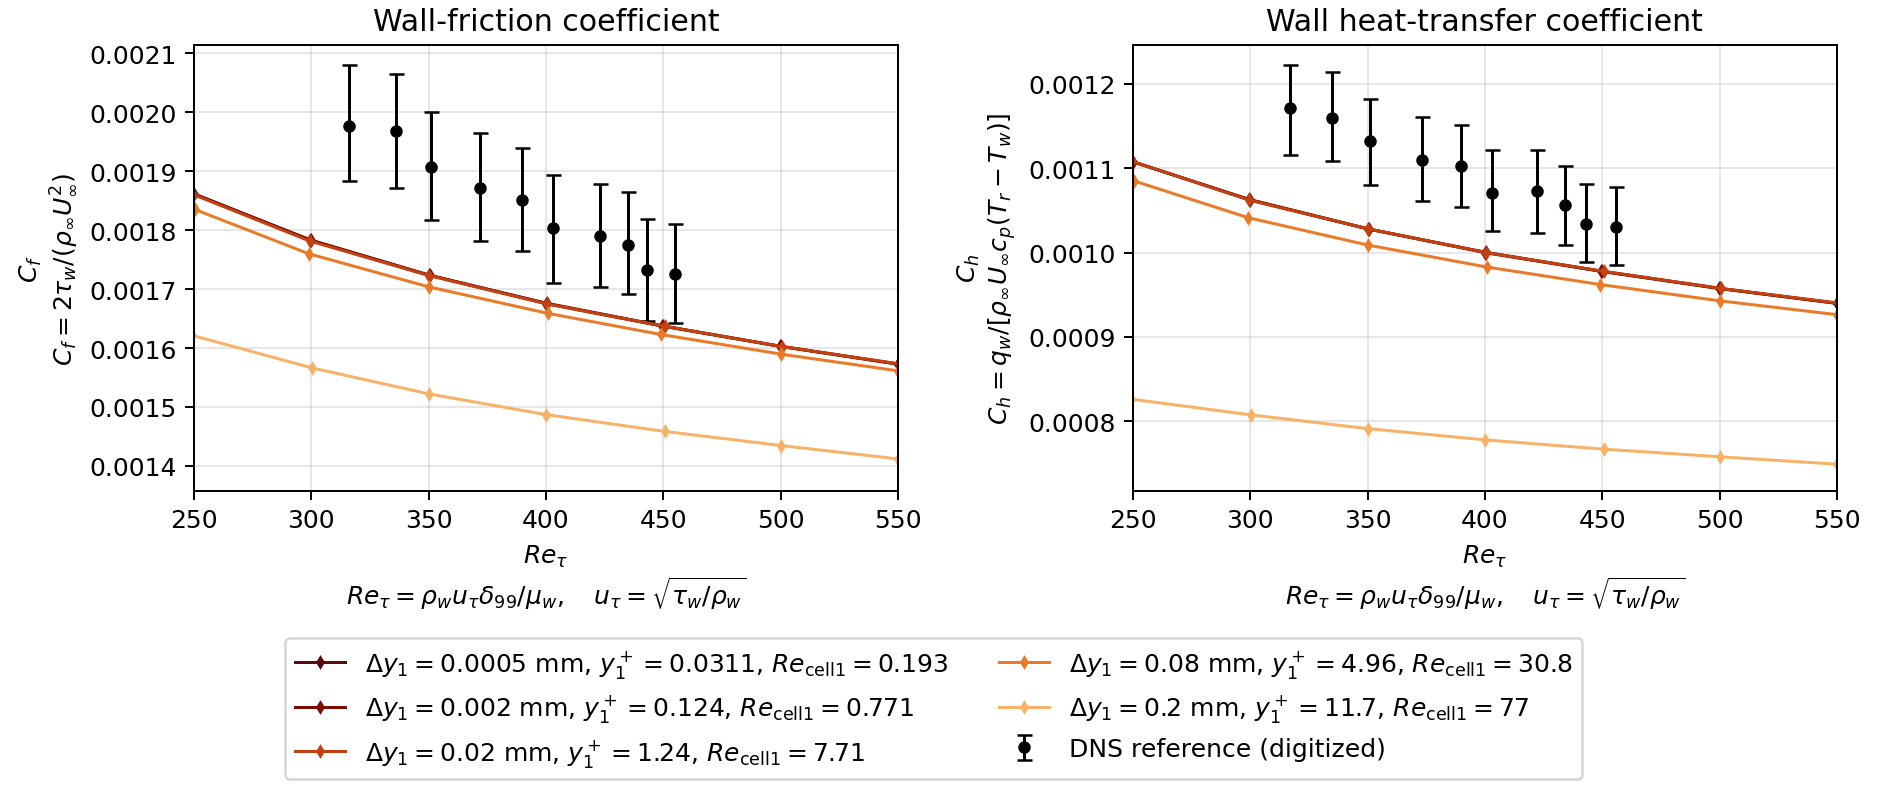
\includegraphics[width=\linewidth]{06_Eval_Methodology/06_Figures/SA_wall_coefficients_vs_dns.png}
    \caption[M6Tw025: first-cell mesh sensitivity with SA]{First-cell mesh sensitivity of the SA predictions for M6Tw025: skin-friction coefficient \(C_f\) (left) and Stanton number \(C_h\) (right) versus \(Re_\tau\), with fixed downstream spacing \(\Delta x=5\,\mathrm{mm}\). Coloured curves show the different first-cell thicknesses \(\Delta y_1\); black symbols denote the digitized DNS reference~\cite{zhang2018direct}. The \(y_1^+\) values reported in the legend are evaluated at each mesh's DNS-matched station, defined by \(Re_{\delta2}=1135\), rather than representing a constant value along the plate.}
    \label{fig:evaluation:SA-mesh-convergence-behaviour}
\end{figure}

\begin{figure}[H]
    \centering
    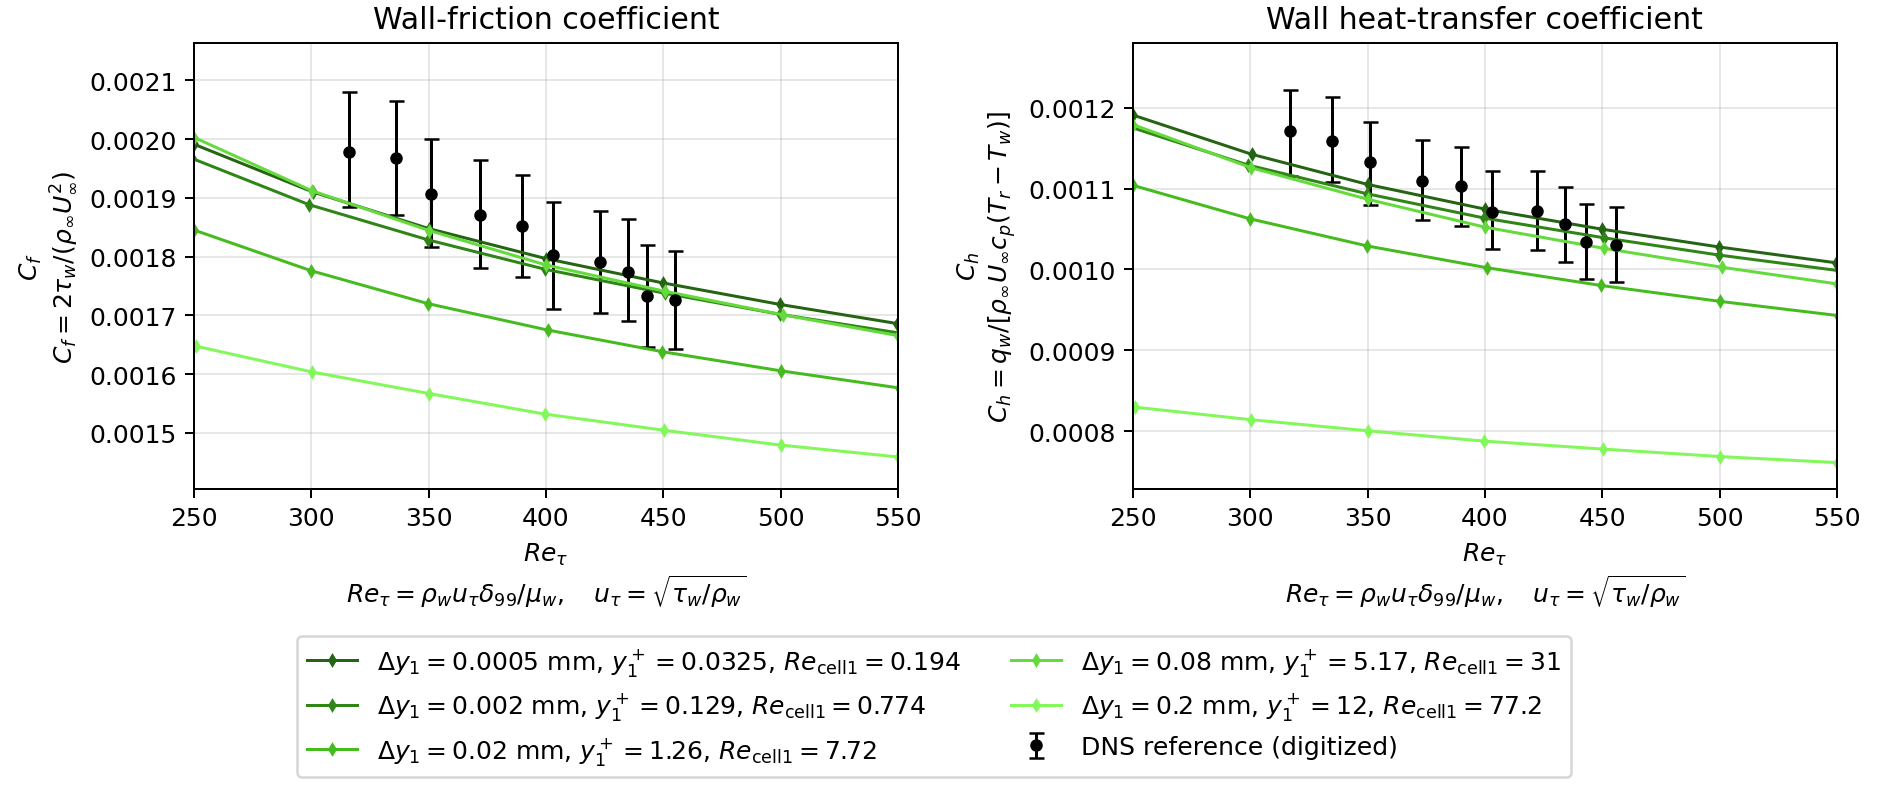
\includegraphics[width=\linewidth]{06_Eval_Methodology/06_Figures/kwSST_wall_coefficients_vs_dns.png}
    \caption[M6Tw025: first-cell mesh sensitivity with SST]{First-cell mesh sensitivity of the \(k\)--\(\omega\) SST predictions for M6Tw025: skin-friction coefficient \(C_f\) (left) and Stanton number \(C_h\) (right) versus \(Re_\tau\), with fixed downstream spacing \(\Delta x=5\,\mathrm{mm}\). Coloured curves show the different first-cell thicknesses \(\Delta y_1\); black symbols denote the digitized DNS reference~\cite{zhang2018direct}. The \(y_1^+\) values reported in the legend are evaluated at each mesh's DNS-matched station, defined by \(Re_{\delta2}=1135\), rather than representing a constant value along the plate.}
    \label{fig:evaluation:SST-mesh-convergence-behaviour}
\end{figure}

Appendix~\ref{app:zpg:mesh-convergence} extends the wall-normal refinement study to all twelve ZPG flat-plate cases. Streamwise-refinement tests for M6Tw025 showed negligible sensitivity of heat-flux and skin-friction to the downstream spacing when the leading edge was refined. The remaining mesh studies therefore focus on the wall-normal direction. They report skin-friction and, for the isothermal cases, heat-transfer against \(y_1^+\) and \(Re_{\mathrm{cell1}}\) at the DNS-matched downstream stations. For the investigated hypersonic cold-wall cases, these results support \(Re_{\mathrm{cell1}}\le1\) as a practical resolution guideline, particularly for SST, in preference to relying on \(y_1^+\le1\) alone.
\par\medskip

The wall-gradient approximation provides a plausible explanation for this stringent resolution requirement. As discussed in Section~\ref{sec:openFOAM_qw_tauw}, OpenFOAM/HiSA evaluates the wall gradients from the difference between the wall value and the first off-wall cell value. Accurate wall fluxes therefore require this secant to approximate the local wall derivative. Placing the first cell within the nominal viscous sublayer is insufficient if the velocity or temperature gradient varies appreciably across that distance. The cold-wall profile shapes in Figures~\ref{fig:background:dns-velocity-profiles} and~\ref{fig:background:dns-temperature-profiles} motivate this distinction between resolving a profile and resolving its wall slope. The mesh studies establish the numerical basis for the wall-resolved model comparisons in Section~\ref{sec:comparative:zpg:wall-resolved-baselines}, where agreement with the DNS reference is assessed separately there.

\section{Criteria for successful performance}
\label{sec:evaluation:success-criteria}
% Writing prerequisite for Chapter 7: finalize the accuracy targets and their
% rationale, including the plotted +/-5% DNS-relative target band. Distinguish
% an engineering acceptance target from DNS uncertainty or reporting precision.

Section~\ref{sec:evaluation:benchmark-cases} identifies uncertainties and ambiguities in the DNS references used for this assessment. In comparing RANS predictions with these references, as in related assessments such as that of Xue et al.~\cite{xue2024assessment}, a quantitative accuracy target is needed. This work adopts a \(\pm5\%\) DNS-relative error band as the target for wall-resolved heat-flux predictions. This band is an engineering acceptance criterion and neither represents the uncertainty of the individual DNS references nor defines a statistical confidence interval. The reference limitations discussed above must therefore be considered when judging agreement within this band.
\par\medskip

The target is motivated by the relative simplicity of attached ZPG flat-plate boundary layers and the accuracy already achieved by analytical approaches. Hasan et al.~\cite[Figure~2]{manzoor2024estimating}, for example, report heat-transfer errors mostly within \(\pm8\%\), with a maximum of \(10.3\%\), for a dataset that includes several of the benchmarks investigated here. Wall-resolved RANS should therefore aim to improve on this level of accuracy. For wall-function calculations, \(\pm10\%\) is adopted as the minimum acceptable heat-flux accuracy: for these ZPG cases, larger errors would leave the additional computational cost of CFD without a corresponding gain in heat-flux accuracy over the analytical approach.
\par\medskip

Beyond error magnitude, engineering use also requires an assessment of how consistently a method behaves. A systematic bias is easier to account for than an error that varies strongly and non-monotonically with sampling height or mesh spacing. This distinction helps frame the three analyses that follow: wall-resolved RANS discrepancies in Section~\ref{sec:comparative:zpg:wall-resolved-baselines}, wall-function closure errors in Section~\ref{sec:comparative:zpg:cross-comparison}, and spatial-discretization errors in Section~\ref{subsec:comparative:zpg:yplus-sensitivity}. For example, the wall-resolved heat-flux discrepancy for a given case may act primarily as a bias, while the closure and spatial discretization may introduce more irregular variations as the sampling height and mesh spacing change. The following sections examine these behaviours alongside the quantitative accuracy targets.


\chapter{Isolation of errors in wall-function predictions}
\label{chap:comparative-evaluation} 

The motivation for using wall functions is to reduce the near-wall resolution required for aerothermal predictions without sacrificing the accuracy needed for thermal design. As outlined in Chapter~\ref{chap:introduction}, assessing that accuracy requires more than comparing a wall-function CFD result with a reference heat-flux. The result depends on the wall-function closure, the turbulence model supplying its off-wall state, and the discretization of the remaining boundary layer. A discrepancy in any one of these components can obscure the performance of the others.
\par\medskip

This chapter therefore examines the zero-pressure-gradient (ZPG) flat-plate benchmarks introduced in Chapter~\ref{chap:evaluation-methodology} through successive diagnostic comparisons. Section~\ref{sec:comparative:zpg:wall-resolved-baselines} first establishes the wall-resolved RANS results and distinguishes accuracy in wall shear and heat-transfer from agreement in boundary layer profiles. Section~\ref{sec:comparative:zpg:cross-comparison} then evaluates the wall-function closures on prescribed profiles, removing feedback from the coupled CFD calculation. Section~\ref{subsec:comparative:zpg:yplus-sensitivity} examines the additional sensitivity introduced by conventional wall-function meshes and develops a boundary layer-informed spacing criterion. Finally, Section~\ref{subsec:comparative:zpg:fitted-closure} combines controlled mesh resolution with reference-fitted closures to determine how closely the wall-function calculation can recover its wall-resolved baseline.
\par\medskip

Figure~\ref{fig:wall_function_error_overview} summarizes this diagnostic sequence and the influences examined at each step. The implemented Li and Griffin wall functions are coupled to Spalart--Allmaras (SA), as described in Sections~\ref{sec:wall-functions:gao-li} and~\ref{sec:wall-functions:griffin}. Their coupled results are consequently compared with the corresponding wall-resolved SA calculation. The wall-resolved assessment additionally includes the widely used \(k\)--\(\omega\) SST model to examine whether the observed limitations are specific to SA. The objective is to identify the dominant discrepancies and their interactions, rather than to assume that the total error can be separated into independent additive contributions.

\begin{figure}[H]
    \centering
    % Figure provenance (WSL; absolute paths):
    %   Figure: /mnt/c/Users/MichaelGnadlinger/OneDrive - Hypersonica/Hypersonica Team - Documents/02 Technical/03 Flight physics/16 Theses/2026/01 Gnadl/Docs_and_Presentations/Thesis_tex/thesis/07_Error_Isolation_Results/Figures/07_error_overview.png
    %   Source artwork: /mnt/c/Users/MichaelGnadlinger/OneDrive - Hypersonica/Hypersonica Team - Documents/02 Technical/03 Flight physics/16 Theses/2026/01 Gnadl/Docs_and_Presentations/Final_Maybe_Final.pptx
    %   Python script: Not applicable: native PowerPoint artwork.
    %   Data / simulation roots (high-level):
    %     Not applicable: qualitative synthesis of this chapter; no numerical dataset.
    %   Note: Conceptual diagram: matching native artwork is on slide 6 of Final_Maybe_Final.pptx (also slide 3
    %     of Weekly 260910.pptx).
    %   Note: No separate WSL export is recorded; the figure path above is the retained manuscript screenshot.
    % End figure provenance.
    % Replacement (2026-10-19): native LaTeX/TikZ roadmap below; the original
    % PowerPoint screenshot and its provenance above are retained for context.
    % Native vector replacement for the PowerPoint overview retained as
% 07_error_overview.png. This is a qualitative roadmap, not a data figure.
% Uses the thesis font, TUM colours and TikZ already loaded by tumbook.
% Section references are resolved by the manuscript build.
\begingroup
\begin{tikzpicture}[
    x=\linewidth, y=1cm,
    stage/.style={circle, draw=TUMBlueDark, fill=white,
        line width=.65pt, minimum size=6.5mm, inner sep=0pt,
        font=\small\bfseries, text=TUMBlueDark},
    heading/.style={anchor=north west, inner sep=0pt, align=left,
        text width=.32\linewidth, font=\small\bfseries},
    detail/.style={anchor=north west, inner sep=0pt, align=left,
        text width=.57\linewidth, font=\small},
    sectionref/.style={anchor=north west, inner sep=0pt,
        font=\footnotesize, text=TUMGrayDark}
]
    % The spine indicates reading order, not an additive error decomposition.
    \path[use as bounding box] (0,.15) rectangle (1,-6.4);
    \fill[TUMBlue!5] (0,-4.78) rectangle (1,-6.4);
    \draw[TUMGrayLight, line width=.5pt] (.085,-1.45) -- (1,-1.45);
    \draw[TUMGrayLight, line width=.5pt] (.085,-3.10) -- (1,-3.10);
    \draw[TUMGrayLight, line width=.5pt] (.085,-4.75) -- (1,-4.75);
    \draw[->, TUMBlueDark!65, line width=.6pt] (.027,-.51) -- (.027,-1.47);
    \draw[->, TUMBlueDark!65, line width=.6pt] (.027,-2.16) -- (.027,-3.12);
    \draw[->, TUMBlueDark!65, line width=.6pt] (.027,-3.81) -- (.027,-4.77);

    \node[stage] at (.027,-.18) {1};
    \node[heading] at (.085,0) {Wall-resolved baseline};
    \node[sectionref] at (.085,-.48)
        {Section~\ref{sec:comparative:zpg:wall-resolved-baselines}};
    \node[detail] at (.42,0)
        {SA and \(k\)--\(\omega\) SST compared with DNS.\\[2pt]
         Wall shear, heat flux and boundary layer profiles.};

    \node[stage] at (.027,-1.83) {2};
    \node[heading] at (.085,-1.65) {Wall-function closures};
    \node[sectionref] at (.085,-2.13)
        {Section~\ref{sec:comparative:zpg:cross-comparison}};
    \node[detail] at (.42,-1.65)
        {Li and Griffin inverted on prescribed profiles.\\[2pt]
         Momentum and thermal relations; sensitivity to\\
         sampling height, profiles and reference states.};

    \node[stage] at (.027,-3.48) {3};
    \node[heading] at (.085,-3.3) {Spatial discretization};
    \node[sectionref] at (.085,-3.78)
        {Section~\ref{subsec:comparative:zpg:yplus-sensitivity}};
    \node[detail] at (.42,-3.3)
        {Conventional and boundary layer-informed meshes.\\[2pt]
         Internal-face viscous-gradient reconstruction\\
         and transport-coefficient interpolation.};

    \node[stage] at (.027,-5.13) {4};
    \node[heading] at (.085,-4.95) {Recovery test};
    \node[sectionref] at (.085,-5.43)
        {Section~\ref{subsec:comparative:zpg:fitted-closure}};
    \node[detail] at (.42,-4.95)
        {Reference-fitted Li closure on informed meshes.\\[2pt]
         Recovery of the resolved SA wall quantities\\
         for LowH\_M3.};
\end{tikzpicture}
\endgroup

    \caption[Diagnostic sequence for the wall-function error assessment]{Diagnostic sequence for the attached ZPG flat-plate assessment. The comparisons distinguish interacting influences rather than independent additive error contributions. The final, reference-conditioned test assesses recovery of the resolved SA result for LowH\_M3; its discrepancy from DNS remains.}
    \label{fig:wall_function_error_overview}
\end{figure}

\section{Evaluation logic and reference hierarchy}
\label{sec:comparative:zpg:reference-data}

The wall-resolved assessment uses the twelve ZPG flat-plate cases listed in Table~\ref{tab:evaluation:selected-cases}. Their gas and transport models, wall conditions, and reference-data limitations are specified in Section~\ref{sec:evaluation:benchmark-cases}. The detailed wall-function comparisons focus on M6Tw025 and LowH\_M3. The reason for this selection follows from the profile assessment in Section~\ref{subsec:comparative:zpg:case-selection}. These two cases provide complementary evidence, rather than a controlled variation of a single physical parameter outlined in detail in Section~\ref{subsec:comparative:zpg:case-selection}.
\par\medskip

Three comparisons are distinguished throughout the chapter, as summarized in Table~\ref{tab:erriso:reference-hierarchy}. The first assesses the wall-resolved RANS calculation against the published DNS reference. The second supplies a fixed boundary layer profile to a standalone wall-function solver and compares the recovered wall quantities with those associated with that profile. The third evaluates the coupled wall-function CFD result against both DNS and the corresponding wall-resolved SA solution.

\begin{table}[!htbp]
    \centering
    \caption{Reference hierarchy used to distinguish RANS discrepancies, conditional wall-function closure errors, and the additional discrepancies of the coupled calculation.}
    \label{tab:erriso:reference-hierarchy}
    \small
    \begin{tabular}{@{}p{0.22\linewidth}p{0.29\linewidth}p{0.40\linewidth}@{}}
        \toprule
        Calculation & Comparison reference & Purpose \\
        \midrule
        Wall-resolved RANS & Published DNS wall quantities and profiles & Establish the resolved baseline and assess turbulence and thermal modelling. \\
        \addlinespace
        Standalone wall function & Wall quantities belonging to the prescribed profile; common DNS reference for the paired M6Tw025 test & Assess closure accuracy and sensitivity to the supplied profile without coupled-flow feedback. \\
        \addlinespace
        Coupled wall-function CFD & DNS and wall-resolved SA at the comparison station & Assess overall accuracy and departures from the resolved baseline as mesh and closure treatment change. \\
        \bottomrule
    \end{tabular}
\end{table}

The comparison stations follow the matching procedure in Section~\ref{subsec:evaluation:matching-station}. Wall-resolved RANS is matched to the DNS through the reported momentum-thickness Reynolds number, with definitions retained consistently for each dataset. Wall-function CFD is then evaluated at the same physical downstream station as its wall-resolved SA baseline. Matching the coarse wall-function solution independently through a boundary layer integral would introduce an additional dependence on how that integral is reconstructed on the coarse mesh. Holding the downstream station fixed instead exposes changes in boundary layer development caused by the coupled wall treatment.
\par\medskip

For a quantity \(Q\), the signed relative error is the difference between the calculated value \(Q_A\) and the reference value \(Q_B\), divided by the reference value:
\begin{equation}
    e_{A/B}(Q)=\frac{Q_A-Q_B}{Q_B},
    \qquad Q_B\ne0,
    \label{eq:erriso:signed-relative-error}
\end{equation}
Both values must use the same definition and sign convention. The plots express this error as a percentage, \(100e_{A/B}\). A dimensional wall quantity and its corresponding coefficient have the same relative error only if the calculated and reference values use the same normalization. The published coefficient definitions and reconstructed DNS values are given in Table~\ref{tab:evaluation:dns-reference-values}. Relative heat-flux errors are undefined for an exactly adiabatic reference, and the M6Tw076 heat-flux comparison is excluded from quantitative assessment because of the reference limitations discussed in Section~\ref{sec:evaluation:benchmark-cases}.
\par\medskip

The wall-resolved mesh studies in Section~\ref{sec:evaluation:mesh-families-yplus} and Appendix~\ref{app:zpg:mesh-convergence} provide the resolution evidence for the wall-resolved baselines. Their interpretation also relies on the numerical methods and convergence criteria in Sections~\ref{sec:numerical-framework:discretization} and~\ref{sec:numerical-framework:convergence}.

\section{Wall-resolved turbulence-model results}
\label{sec:comparative:zpg:wall-resolved-baselines}

The first comparison establishes the accuracy of the flow calculation before a wall function is introduced. Wall-resolved Spalart--Allmaras (SA) and \(k\)--\(\omega\) SST simulations are evaluated against the selected DNS references using the matching procedure and transport properties in Section~\ref{sec:evaluation:benchmark-cases}. Both momentum closures use the same gradient-diffusion thermal closure with \(Pr_t=0.9\), unless explicitly stated otherwise. The SA calculations employ the corrected compressible implementation described in Section~\ref{subsec:ext:spalart-allmaras-of-correction}. SA is also the underlying momentum closure for the coupled Li and Griffin calculations investigated subsequently, whereas SST provides a general comparison with another widely used RANS model.
\par\medskip

The mesh studies in Section~\ref{sec:evaluation:mesh-families-yplus}, provide the basis for using these solutions as wall-resolved references. Their differences from DNS measure the accuracy of the complete resolved RANS calculation, including its thermal closure and remaining numerical and reference-data uncertainties. In the later wall-function comparisons, the corresponding SA solution serves as the baseline against which the additional effects of the wall closure and its coupling to the discretized flow are assessed.

\subsection{Prediction of wall heat-flux and skin-friction}
\label{subsec:comparative:zpg:wr-wall-fluxes}

Table~\ref{tab:wall-resolved:coefficients} reports the, wall coefficients and signed relative errors for both models, across the investigated ZPG FPs at the respectively \(Re_{\delta2}\) matched station. DNS rows give the reference values used to calculate the errors, complementing the published-data overview in Table~\ref{tab:evaluation:dns-reference-values}. The CFD stations agree with the nominal DNS targets to within \(0.1\%\). Overall Table~\ref{tab:wall-resolved:coefficients} shows a relative errors against DNS range from \(-14.8\%\) to \(+13.7\%\) in heat-flux and from \(-18.5\%\) to \(+12.5\%\) in wall shear stress for SA, compared with \(-12.8\%\) to \(+20.6\%\) and \(-17.1\%\) to \(+15.6\%\), respectively, for \(k\)--\(\omega\) SST, across the investigated cases. Neither turbulence model consistently outperforms the other across the investigated cases and wall quantities.

% Table provenance (WSL; absolute paths):
%   /home/mgnadlinger/Duan_DNS_ZPGFP/dns_comparison_{SA,kwSST}/scalar_error_summary.csv
%   /home/mgnadlinger/Zhang_DNS_ZPGFP/dns_comparison_{SA,kwSST}/scalar_error_summary.csv
%   /home/mgnadlinger/Huang_DNS_ZPGFP/dns_comparison_{SA,kwSST}/scalar_error_summary.csv
%   Actual stations checked against the curated results.json files and the combined
%   SA/kwSST profile exports used by the main text and Appendix_ZPG.
%   M5T1 uses the corrected Tw=228.1 K run, also used by its appendix profile.
%   Reproducible extraction and checks: tmp/wall_resolved_table/ (workspace root).
%   RANS -Bq uses the same native Re_delta2-matched results.json samples:
%     /home/mgnadlinger/Zhang_DNS_ZPGFP/{SA,kwSST}_Prt0p9/<case>/postProcessing/TM_ZPGFP/<time>/results.json
%     /home/mgnadlinger/Huang_DNS_ZPGFP/{SA,kwSST}_Prt0p9/M11Tw20/postProcessing/TM_ZPGFP/<time>/stations/<BL>/results.json
%   -Bq = heat_flux_to_wall/(rho_wall*Cp*u_tau*T_wall), with heat_flux_to_wall
%   equal to minus the OpenFOAM wallHeatFlux output. Each RANS wall state is used.
%   Exact paths, times, wall inputs and source hashes: tmp/wall_resolved_table/bq_results_audit.json.
%   Reproduction: tmp/wall_resolved_table/extract_bq.py (workspace root).
% End table provenance.
\begingroup
\small
\sisetup{detect-weight=true}
\setlength{\tabcolsep}{5pt}
\begin{longtable}{@{}ll
    S[table-format=4.1]
    S[table-format=1.5]
    S[table-format=+2.2]
    S[table-format=1.5]
    S[table-format=+2.2]
    S[table-format=1.4]@{}}
    \caption[Wall-resolved wall coefficients and signed DNS errors]{Wall-resolved SA and \(k\)--\(\omega\) SST results at \(Pr_t=0.9\), with the DNS values used for comparison (see Table~\ref{tab:evaluation:dns-reference-values}). The \(Re_{\delta2}\) column gives the nominal target for DNS and the actual sampled value for each CFD solution. Errors \(\varepsilon_f\) and \(\varepsilon_h\) are \(100(C_{\mathrm{RANS}}-C_{\mathrm{DNS}})/C_{\mathrm{DNS}}\) for \(C_f\) and \(C_h\), respectively. The \(-B_q\) column gives Zhang~\cite[Table~2]{zhang2018direct} and Huang~\cite[Table~3]{huang2020simulation} DNS values and corresponding RANS values \(q_{\mathrm{to\,wall}}/(\rho_w c_p u_\tau T_w)\), using heat-flux positive into the wall and each solution's wall state. Entries for \(C_h\) and \(\varepsilon_h\) are omitted for the adiabatic references M5T5 and M2p5 and for M6Tw076; these omissions do not imply zero RANS heat-flux.}\label{tab:wall-resolved:coefficients}\\
    \toprule
    Case / station & Model & {\(Re_{\delta2}\)} & {\(10^3 C_f\)} & {\(\varepsilon_f\,[\%]\)} & {\(10^3 C_h\)} & {\(\varepsilon_h\,[\%]\)} & {\(-B_q\)} \\
    \midrule
    \endfirsthead
    \multicolumn{8}{@{}l}{\tablename~\thetable\ (continued)}\\
    \toprule
    Case / station & Model & {\(Re_{\delta2}\)} & {\(10^3 C_f\)} & {\(\varepsilon_f\,[\%]\)} & {\(10^3 C_h\)} & {\(\varepsilon_h\,[\%]\)} & {\(-B_q\)} \\
    \midrule
    \endhead
    \midrule
    \multicolumn{8}{r@{}}{Continued on next page}\\
    \endfoot
    \bottomrule
    \endlastfoot
    \multicolumn{8}{@{}l}{\textit{Martin--Duan Part 2}}\\*
    \multirow{3}{*}{M5T1} & \textbf{DNS} & \bfseries 1538.4 & \bfseries 2.46 & {\textbf{\textemdash}} & \bfseries 1.39 & {\textbf{\textemdash}} &  \\*
     & SA & 1538.5 & 2.0055 & -18.48 & 1.1839 & -14.83 &  \\*
     & SST & 1538.4 & 2.2824 & -7.22 & 1.3429 & -3.39 &  \\
    \addlinespace[3pt]
    \multirow{3}{*}{M5T2} & \textbf{DNS} & \bfseries 1521.5 & \bfseries 2.05 & {\textbf{\textemdash}} & \bfseries 1.14 & {\textbf{\textemdash}} &  \\*
     & SA & 1520.8 & 1.7334 & -15.45 & 1.0144 & -11.02 &  \\*
     & SST & 1522.2 & 1.7967 & -12.35 & 1.0531 & -7.62 &  \\
    \addlinespace[3pt]
    \multirow{3}{*}{M5T3} & \textbf{DNS} & \bfseries 1524.7 & \bfseries 1.81 & {\textbf{\textemdash}} & \bfseries 0.977 & {\textbf{\textemdash}} &  \\*
     & SA & 1525.0 & 1.5229 & -15.86 & 0.8763 & -10.30 &  \\*
     & SST & 1525.5 & 1.5003 & -17.11 & 0.8697 & -10.98 &  \\
    \addlinespace[3pt]
    \multirow{3}{*}{M5T4} & \textbf{DNS} & \bfseries 1526.4 & \bfseries 1.5 & {\textbf{\textemdash}} & \bfseries 0.839 & {\textbf{\textemdash}} &  \\*
     & SA & 1525.9 & 1.3674 & -8.84 & 0.7545 & -10.07 &  \\*
     & SST & 1526.2 & 1.3018 & -13.22 & 0.7320 & -12.76 &  \\
    \addlinespace[3pt]
    \multirow{3}{*}{M5T5} & \textbf{DNS} & \bfseries 1536.8 & \bfseries 1.28 & {\textbf{\textemdash}} & {\textbf{\textemdash}} & {\textbf{\textemdash}} &  \\*
     & SA & 1537.3 & 1.1912 & -6.94 & {\textemdash} & {\textemdash} &  \\*
     & SST & 1536.8 & 1.1032 & -13.81 & {\textemdash} & {\textemdash} &  \\
    \addlinespace[3pt]
    \multicolumn{8}{@{}l}{\textit{Martin--Duan Part 4}}\\*
    \multirow{3}{*}{LowH\_M3} & \textbf{DNS} & \bfseries 1554.5 & \bfseries 3.12 & {\textbf{\textemdash}} & \bfseries 1.82 & {\textbf{\textemdash}} &  \\*
     & SA & 1554.4 & 2.8950 & -7.21 & 1.7187 & -5.56 &  \\*
     & SST & 1555.0 & 3.5183 & +12.77 & 2.0712 & +13.80 &  \\
    \addlinespace[3pt]
    \multicolumn{8}{@{}l}{\textit{Zhang}}\\*
    \multirow{3}{*}{M2p5} & \textbf{DNS} & \bfseries 1657 & \bfseries 2.3125 & {\textbf{\textemdash}} & {\textbf{\textemdash}} & {\textbf{\textemdash}} & {\textbf{\textemdash}} \\*
     & SA & 1658.0 & 2.1858 & -5.48 & {\textemdash} & {\textemdash} & {\textemdash} \\*
     & SST & 1656.5 & 2.0949 & -9.41 & {\textemdash} & {\textemdash} & {\textemdash} \\
    \addlinespace[3pt]
    \multirow{3}{*}{M6Tw025} & \textbf{DNS} & \bfseries 1135 & \bfseries 1.7043 & {\textbf{\textemdash}} & \bfseries 1.0215 & {\textbf{\textemdash}} & \bfseries 0.14 \\*
     & SA & 1135.3 & 1.6172 & -5.11 & 0.9659 & -5.44 & 0.1320 \\*
     & SST & 1135.8 & 1.7563 & +3.05 & 1.0507 & +2.86 & 0.1374 \\
    \addlinespace[3pt]
    \multirow{3}{*}{M6Tw076} & \textbf{DNS} & \bfseries 1746 & \bfseries 0.99785 & {\textbf{\textemdash}} & {\textbf{\textemdash}} & {\textbf{\textemdash}} & \bfseries 0.02 \\*
     & SA & 1746.2 & 1.0120 & +1.42 & {\textemdash} & {\textemdash} & {\textemdash} \\*
     & SST & 1746.2 & 0.9419 & -5.60 & {\textemdash} & {\textemdash} & {\textemdash} \\
    \addlinespace[3pt]
    \multirow{3}{*}{M8Tw048} & \textbf{DNS} & \bfseries 1990 & \bfseries 0.76629 & {\textbf{\textemdash}} & \bfseries 0.44856 & {\textbf{\textemdash}} & \bfseries 0.06 \\*
     & SA & 1989.9 & 0.8010 & +4.53 & 0.4710 & +5.01 & 0.0592 \\*
     & SST & 1990.0 & 0.7691 & +0.37 & 0.4563 & +1.73 & 0.0586 \\
    \addlinespace[3pt]
    \multirow{3}{*}{M14Tw018} & \textbf{DNS} & \bfseries 2354 & \bfseries 0.40395 & {\textbf{\textemdash}} & \bfseries 0.24337 & {\textbf{\textemdash}} & \bfseries 0.19 \\*
     & SA & 2354.6 & 0.4545 & +12.52 & 0.2694 & +10.70 & 0.1825 \\*
     & SST & 2354.0 & 0.4668 & +15.57 & 0.2776 & +14.09 & 0.1851 \\
    \addlinespace[3pt]
    \multicolumn{8}{@{}l}{\textit{Huang M11Tw020}}\\*
    \multirow{3}{*}{BL1} & \textbf{DNS} & \bfseries 2204 & \bfseries 0.61 & {\textbf{\textemdash}} & \bfseries 0.36 & {\textbf{\textemdash}} & \bfseries 0.164 \\*
     & SA & 2204.5 & 0.6332 & +3.80 & 0.3760 & +4.44 & 0.1647 \\*
     & SST & 2203.2 & 0.6623 & +8.57 & 0.3941 & +9.46 & 0.1683 \\
    \addlinespace[3pt]
    \multirow{3}{*}{BL2} & \textbf{DNS} & \bfseries 3419 & \bfseries 0.55 & {\textbf{\textemdash}} & \bfseries 0.316 & {\textbf{\textemdash}} & \bfseries 0.154 \\*
     & SA & 3418.8 & 0.5820 & +6.40 & 0.3458 & +9.44 & 0.1587 \\*
     & SST & 3418.8 & 0.6140 & +12.24 & 0.3652 & +15.57 & 0.1627 \\
    \addlinespace[3pt]
    \multirow{3}{*}{BL3} & \textbf{DNS} & \bfseries 4390 & \bfseries 0.51 & {\textbf{\textemdash}} & \bfseries 0.29 & {\textbf{\textemdash}} & \bfseries 0.148 \\*
     & SA & 4389.9 & 0.5545 & +8.73 & 0.3296 & +13.66 & 0.1553 \\*
     & SST & 4389.2 & 0.5884 & +15.37 & 0.3499 & +20.64 & 0.1595 \\
    \addlinespace[3pt]
\end{longtable}
\endgroup

Figures~\ref{fig:wall-resolved:kwSST_DNS_ZPG_FPs} and~\ref{fig:wall-resolved:SA_DNS_ZPG_FPs} summarize the signed errors in the skin-friction coefficient \(C_f\) and Stanton number \(C_h\). The two abscissae characterize different aspects of the flow: \(-B_q\) represents wall heat-transfer, while \(M_\tau\) indicates the strength of compressibility associated with the friction velocity. The Figures~\ref{fig:wall-resolved:kwSST_DNS_ZPG_FPs} and~\ref{fig:wall-resolved:SA_DNS_ZPG_FPs} do not reveal any clear correlation in reduction in error with either cold-wall effect or compressibility. Thus from this investigation it is unclear what causes the turbulence models to have such bad performance in predicting the heat-flux and skin-friction on hypersonic flat-plates. These comparisons therefore establish a substantial baseline discrepancy on some of the simplest attached turbulent flows, but do not by themselves identify its physical cause.

\begin{figure}[H]
    \centering
    % Figure provenance (WSL; absolute paths):
    %   Original retained figure: /home/mgnadlinger/ZPG_FP_overview/orig.DNS_Cf_Ch_relative_error_kwSST.png
    %   Updated figure: tmp/wall_resolved_table/figures/DNS_Cf_Ch_relative_error_kwSST.png (workspace root)
    %   Readability replot (2026-10-19): four stacked panels at the printed 170 mm
    %     width, 9.5 pt labels/ticks/legend, and vector PDF output. Exact values and
    %     omissions are retained from the audited 2026-10-14 figures above.
    %     Local regeneration: Figures/WallResolved/plot_wall_coefficient_errors.py
    %     with wall_coefficient_error_data.csv and wall_coefficient_error_provenance.json
    %     in the same directory (paths relative to this chapter).
    %   Python script:
    %     /home/mgnadlinger/ZPG_FP_overview/plot_dns_coefficient_errors.py
    %   Data / simulation roots (high-level):
    %     /home/mgnadlinger/Duan_DNS_ZPGFP/dns_comparison_kwSST
    %     /home/mgnadlinger/Huang_DNS_ZPGFP/dns_comparison_kwSST
    %     /home/mgnadlinger/Zhang_DNS_ZPGFP/dns_comparison_kwSST
    %     /home/mgnadlinger/Duan_DNS_ZPGFP/Martin_Duan_Part2/kwSST_Prt0p9
    %     /home/mgnadlinger/Duan_DNS_ZPGFP/Martin_Duan_Part4/kwSST_Prt0p9/LowH_M3
    %     /home/mgnadlinger/Huang_DNS_ZPGFP/kwSST_Prt0p9/M11Tw20
    %     /home/mgnadlinger/Zhang_DNS_ZPGFP/kwSST_Prt0p9
    %     /home/mgnadlinger/Duan_DNS_ZPGFP/Martin_Duan_Part2/Digitizations
    %     /home/mgnadlinger/Duan_DNS_ZPGFP/Martin_Duan_Part4/Digitizations
    %     /home/mgnadlinger/Huang_DNS_ZPGFP/References
    %     /home/mgnadlinger/Zhang_DNS_ZPGFP/References/Data
    %   Note: Updated on 2026-10-14 from the current curated comparison exports to include
    %     the corrected M5T1 Tw=228.1 K run, consistent with its appendix profile.
    %     Regeneration wrapper: tmp/wall_resolved_table/regenerate_point_only_overviews.py
    %     (workspace root); retains point-only presentation and original legend, without
    %     the trend fits added to the current external plotting script. All other values
    %     agree with the retained orig. export. Numerical audit and input snapshot are
    %     retained in tmp/wall_resolved_table/; original WSL provenance is preserved above.
    % End figure provenance.
    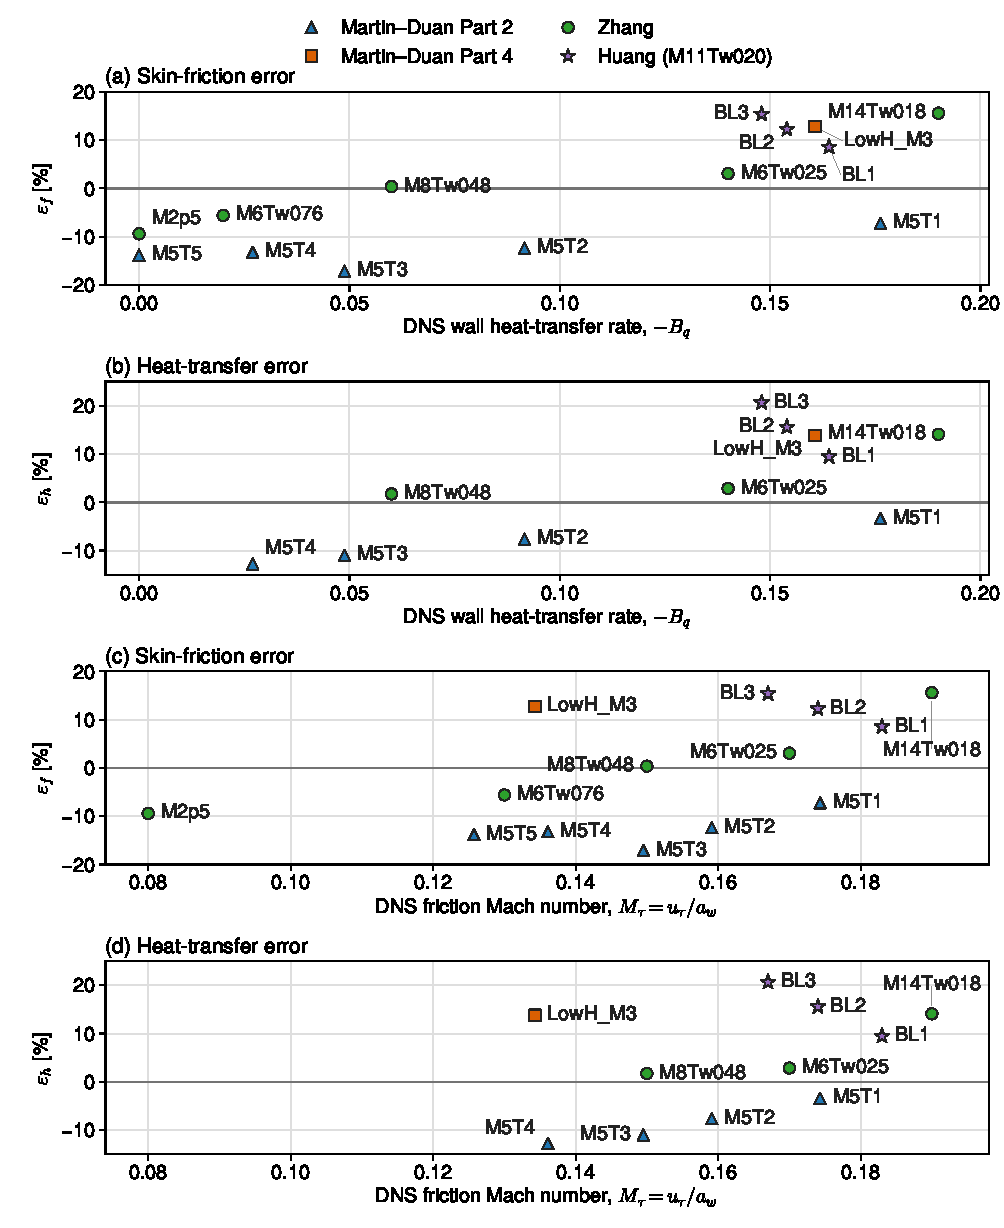
\includegraphics[width=\linewidth]{07_Error_Isolation_Results/Figures/WallResolved/DNS_Cf_Ch_relative_error_kwSST.pdf}
    \caption[Wall-resolved \(k\)--\(\omega\) SST errors in skin-friction and heat-transfer]{Signed relative errors, \(100(C_{\mathrm{RANS}}-C_{\mathrm{DNS}})/C_{\mathrm{DNS}}\), for wall-resolved \(k\)--\(\omega\) SST at \(Pr_t=0.9\). Panels (a,b): errors in the skin-friction coefficient \(C_f\) and Stanton number \(C_h\), respectively, versus the DNS dimensionless wall heat-transfer rate \(-B_q\). Panels (c,d): the corresponding errors versus the DNS friction Mach number \(M_\tau=u_\tau/a_w\). Symbols identify the DNS sources and annotations the cases; BL1--BL3 are three stations of the single Huang case. Heat-transfer errors are omitted for the adiabatic references and M6Tw076. Definitions, matching stations and reference-data limitations follow Section~\ref{sec:evaluation:benchmark-cases}.}
    \label{fig:wall-resolved:kwSST_DNS_ZPG_FPs}
\end{figure}

\begin{figure}[H]
    \centering
    % Figure provenance (WSL; absolute paths):
    %   Original retained figure: /home/mgnadlinger/ZPG_FP_overview/orig.DNS_Cf_Ch_relative_error_SA.png
    %   Updated figure: tmp/wall_resolved_table/figures/DNS_Cf_Ch_relative_error_SA.png (workspace root)
    %   Readability replot (2026-10-19): four stacked panels at the printed 170 mm
    %     width, 9.5 pt labels/ticks/legend, and vector PDF output. Exact values and
    %     omissions are retained from the audited 2026-10-14 figures above.
    %     Local regeneration: Figures/WallResolved/plot_wall_coefficient_errors.py
    %     with wall_coefficient_error_data.csv and wall_coefficient_error_provenance.json
    %     in the same directory (paths relative to this chapter).
    %   Python script:
    %     /home/mgnadlinger/ZPG_FP_overview/plot_dns_coefficient_errors.py
    %   Data / simulation roots (high-level):
    %     /home/mgnadlinger/Duan_DNS_ZPGFP/dns_comparison_SA
    %     /home/mgnadlinger/Huang_DNS_ZPGFP/dns_comparison_SA
    %     /home/mgnadlinger/Zhang_DNS_ZPGFP/dns_comparison_SA
    %     /home/mgnadlinger/Duan_DNS_ZPGFP/Martin_Duan_Part2/SA_Prt0p9
    %     /home/mgnadlinger/Duan_DNS_ZPGFP/Martin_Duan_Part4/SA_Prt0p9/LowH_M3
    %     /home/mgnadlinger/Huang_DNS_ZPGFP/SA_Prt0p9/M11Tw20
    %     /home/mgnadlinger/Zhang_DNS_ZPGFP/SA_Prt0p9
    %     /home/mgnadlinger/Duan_DNS_ZPGFP/Martin_Duan_Part2/Digitizations
    %     /home/mgnadlinger/Duan_DNS_ZPGFP/Martin_Duan_Part4/Digitizations
    %     /home/mgnadlinger/Huang_DNS_ZPGFP/References
    %     /home/mgnadlinger/Zhang_DNS_ZPGFP/References/Data
    %   Note: Updated on 2026-10-14 from the current curated comparison exports to include
    %     the corrected M5T1 Tw=228.1 K run, consistent with its appendix profile.
    %     Regeneration wrapper: tmp/wall_resolved_table/regenerate_point_only_overviews.py
    %     (workspace root); retains point-only presentation and original legend, without
    %     the trend fits added to the current external plotting script. All other values
    %     agree with the retained orig. export. Numerical audit and input snapshot are
    %     retained in tmp/wall_resolved_table/; original WSL provenance is preserved above.
    % End figure provenance.
    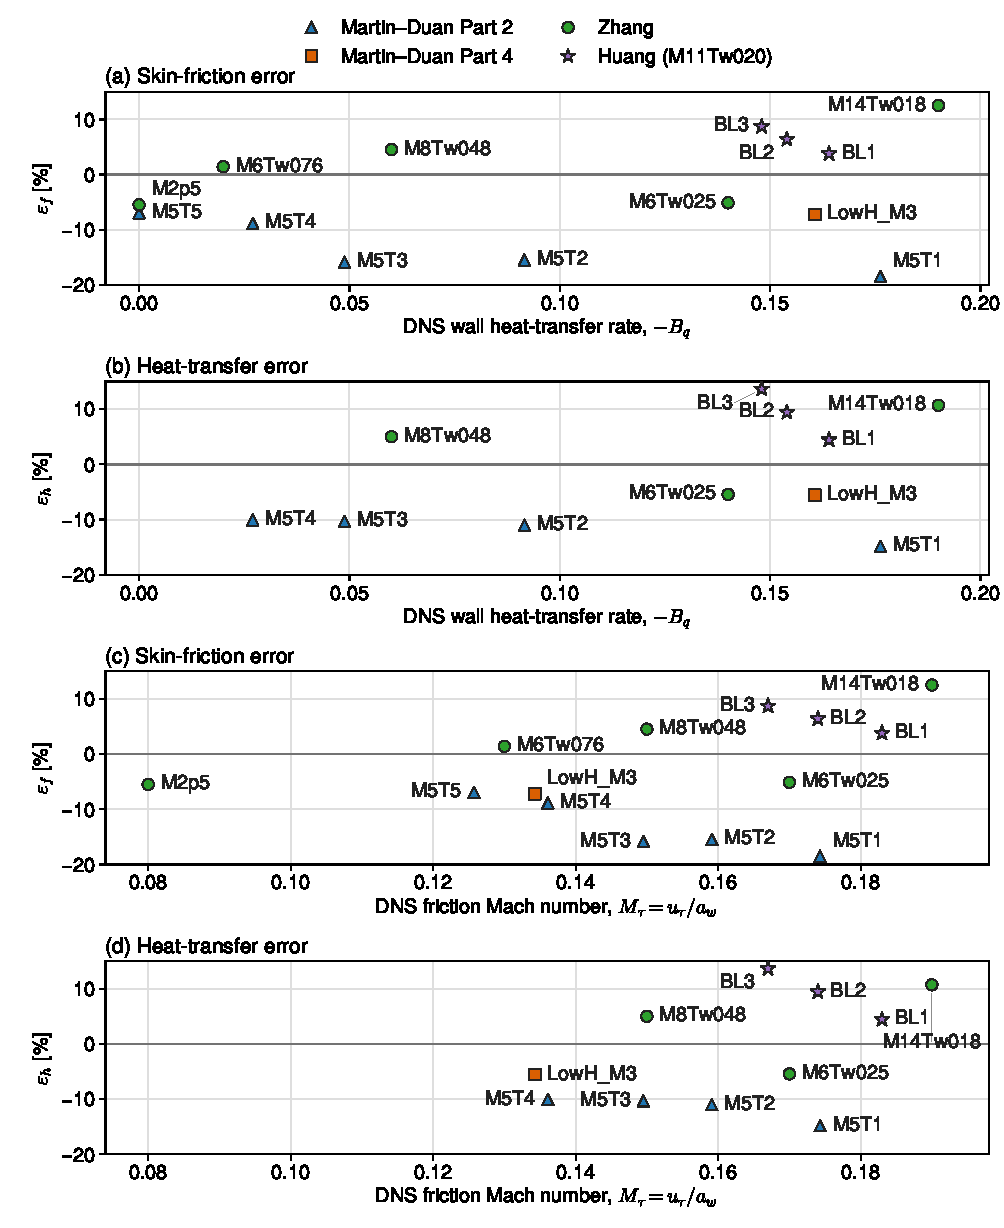
\includegraphics[width=\linewidth]{07_Error_Isolation_Results/Figures/WallResolved/DNS_Cf_Ch_relative_error_SA.pdf}
    \caption[Wall-resolved Spalart--Allmaras errors in skin-friction and heat-transfer]{Signed relative errors for the corrected wall-resolved Spalart--Allmaras model at \(Pr_t=0.9\), using the same references and definitions as Figure~\ref{fig:wall-resolved:kwSST_DNS_ZPG_FPs}. Panels (a,b): errors in \(C_f\) and \(C_h\), respectively, versus DNS \(-B_q\). Panels (c,d): the corresponding errors versus DNS \(M_\tau\). Positive values indicate overprediction of the reference coefficient. Heat-transfer errors are omitted for the adiabatic references and M6Tw076.}
    \label{fig:wall-resolved:SA_DNS_ZPG_FPs}
\end{figure}

\subsection{Boundary layer profiles and temperature--velocity relations}
\label{subsec:comparative:zpg:wr-profiles}

Wall coefficients alone do not show whether the flow supplied to a wall function has the correct internal structure. The detailed profile comparisons therefore examine both velocity and temperature, with particular emphasis on the mean temperature--velocity relation \(T(U)\) introduced in Section~\ref{subsec:background:temperature-velocity}. This relation is directly relevant to the energy closures of the investigated analytical wall functions. A discrepancy in \(T(U)\) implies that a wall closure fitted to DNS and the resolved RANS field need not describe the same relation between thermal and momentum transport, even when their wall heat-fluxes are close.
\par\medskip

Figures~\ref{fig:wall-resolved:M6Tw025_BL_Profile} and~\ref{fig:wall-resolved:LowH_M3_BL_Profile} illustrate the contrast using M6Tw025 and LowH\_M3. Corresponding comparisons for the other ten benchmark cases are provided in Appendix~\ref{app:zpg:wr-profiles}.

\begin{figure}[H]
    \centering
    % Figure provenance (WSL; absolute paths):
    %   Figure: /home/mgnadlinger/Zhang_DNS_ZPGFP/dns_comparison_SA_kwSST/figures/M6Tw025_profiles.png
    %   Python script:
    %     /home/mgnadlinger/Zhang_DNS_ZPGFP/plot_combined_dns_profiles.py
    %   Data / simulation roots (high-level):
    %     /home/mgnadlinger/Zhang_DNS_ZPGFP/SA_Prt0p9/M6Tw025
    %     /home/mgnadlinger/Zhang_DNS_ZPGFP/kwSST_Prt0p9/M6Tw025
    %     /home/mgnadlinger/Zhang_DNS_ZPGFP/References/Data
    %   Print-size replot (2026-10-19):
    %     thesis/07_Error_Isolation_Results/Figures/WallResolved/plot_wall_resolved_profiles.py
    %     Exact plotted coordinates and source hashes retained in adjacent
    %     wall_resolved_profile_data.json and wall_resolved_profile_provenance.json.
    %     Original curves/stations/panel selection preserved; 170 mm PDF, 10.5 pt text.
    % End figure provenance.
    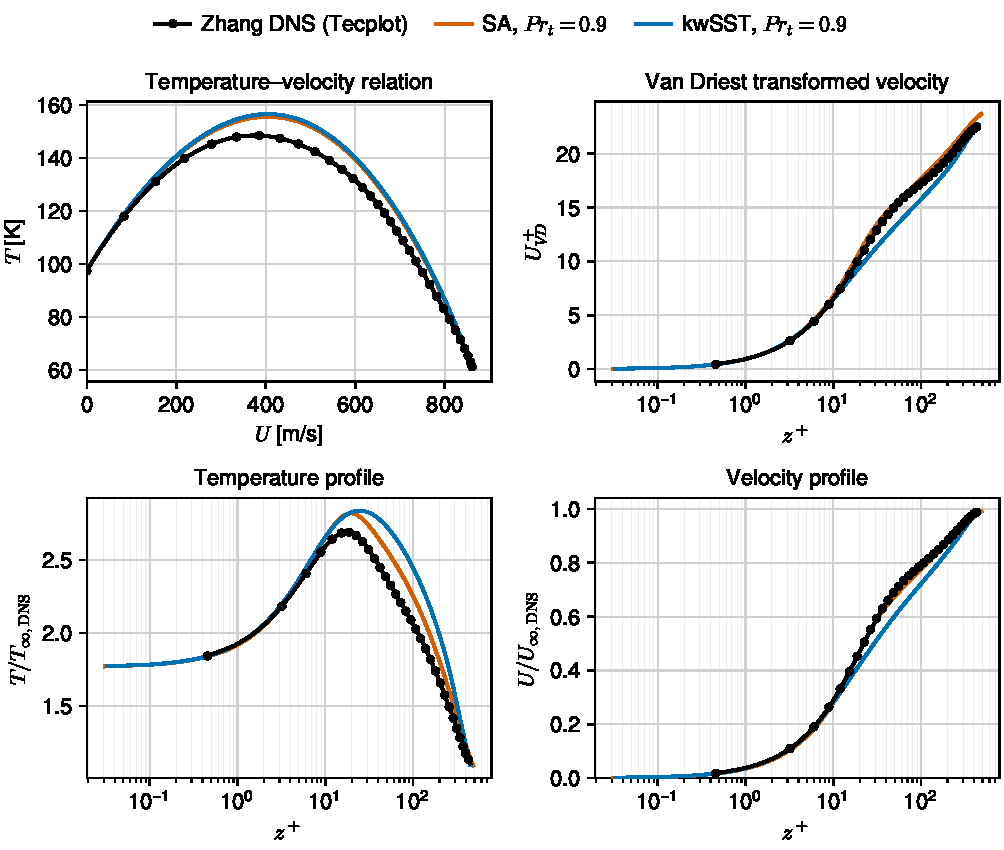
\includegraphics[width=\linewidth]{07_Error_Isolation_Results/Figures/WallResolved/M6Tw025_BL_profiles.pdf}
    \caption[M6Tw025: wall-resolved boundary layer profiles compared with DNS]{Wall-resolved Spalart--Allmaras and \(k\)--\(\omega\) SST profiles for M6Tw025 at \(Pr_t=0.9\), matched at \(Re_{\delta2}=1135\) and compared with Zhang et al.'s digital DNS profiles~\cite{zhang2018direct}. Top: dimensional temperature--velocity relation \(T(U)\) (left) and van Driest--transformed velocity \(U_{\mathrm{VD}}^+\) versus wall distance \(z^+\) (right). Bottom: normalized temperature \(T/T_{\infty,\mathrm{DNS}}\) (left) and velocity \(U/U_{\infty,\mathrm{DNS}}\) (right) versus \(z^+\). Profiles are truncated at their \(99\%\)-velocity boundary layer edge. The thermal maximum is overpredicted by both turbulence models despite differences between their velocity profiles.}
    \label{fig:wall-resolved:M6Tw025_BL_Profile}
\end{figure}

\begin{figure}[H]
    \centering
    % Figure provenance (WSL; absolute paths):
    %   Figure: /home/mgnadlinger/Duan_DNS_ZPGFP/dns_comparison_SA_kwSST/figures/Part4_LowH_M3_profiles.png
    %   Python script:
    %     /home/mgnadlinger/Duan_DNS_ZPGFP/plot_combined_dns_profiles.py
    %   Data / simulation roots (high-level):
    %     /home/mgnadlinger/Duan_DNS_ZPGFP/Martin_Duan_Part4/SA_Prt0p9/LowH_M3
    %     /home/mgnadlinger/Duan_DNS_ZPGFP/Martin_Duan_Part4/kwSST_Prt0p9/LowH_M3
    %     /home/mgnadlinger/Duan_DNS_ZPGFP/Martin_Duan_Part4/Digitizations
    %   Note: Previous thesis PNG cropped the upper two panels of the source export.
    %   Print-size replot (2026-10-19):
    %     thesis/07_Error_Isolation_Results/Figures/WallResolved/plot_wall_resolved_profiles.py
    %     Exact plotted coordinates and source hashes retained in adjacent
    %     wall_resolved_profile_data.json and wall_resolved_profile_provenance.json.
    %     Original curves/stations/panel selection preserved; 170 mm PDF, 10.5 pt text.
    % End figure provenance.
    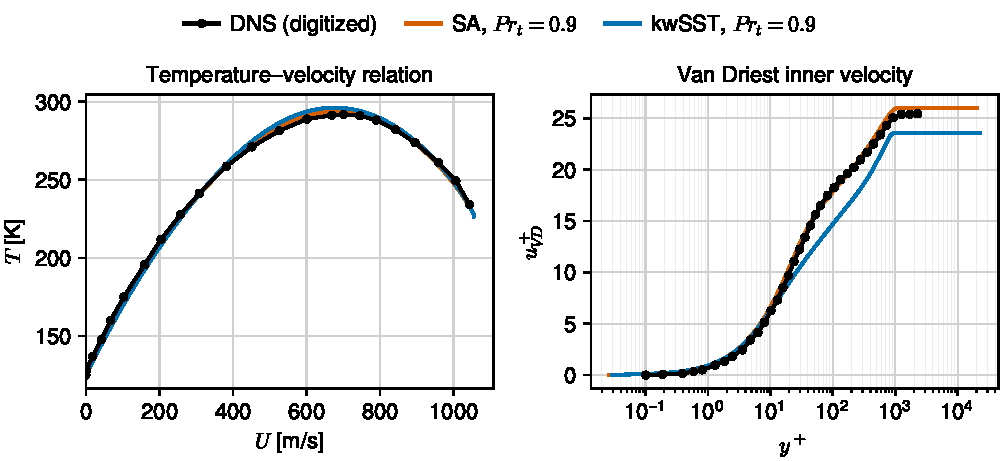
\includegraphics[width=\linewidth]{07_Error_Isolation_Results/Figures/WallResolved/Part4_LowH_M3_BL_profiles.pdf}
    \caption[LowH\_M3: wall-resolved boundary layer profiles compared with DNS]{Wall-resolved Spalart--Allmaras and \(k\)--\(\omega\) SST profiles for Martin--Duan Part~4 LowH\_M3 at \(Re_{\delta2}=1554.5\) and \(Pr_t=0.9\), compared with digitized DNS~\cite{duan2011direct_Part4}. Left: dimensional temperature--velocity relation \(T(U)\). Right: van Driest--transformed velocity \(U_{\mathrm{VD}}^+\) versus wall distance \(y^+\). The DNS wall-normal reconstruction retains the provisional boundary layer-edge endpoint assumption indicated in the plot. Both models closely reproduce the displayed \(T(U)\) relation, while their transformed velocity profiles differ.}
    \label{fig:wall-resolved:LowH_M3_BL_Profile}
\end{figure}

For M6Tw025, both Spalart--Allmaras and \(k\)--\(\omega\) SST overpredict the temperature maximum and the recovering part of the thermal profile (see Figure~\ref{fig:wall-resolved:M6Tw025_BL_Profile}). Their \(T(U)\) curves are very similar, although the transformed velocity profiles and the locations of the thermal maximum in wall units differ. SST's close wall-coefficient agreement (see Figure~\ref{fig:wall-resolved:kwSST_DNS_ZPG_FPs}) consequently coexists with a visibly incorrect thermal profile. SA, meanwhile, follows the displayed velocity profiles comparatively closely despite its thermal discrepancy. Section~\ref{subsec:erriso:rans-profile-influence} tests the consequence for wall-function heating by applying the same Li closure to the DNS and resolved SA profiles.
\par\medskip

The LowH\_M3 case presents the complementary behaviour: both models closely reproduce the displayed \(T(U)\) relation (see Figure~\ref{fig:wall-resolved:LowH_M3_BL_Profile}), yet their wall coefficients retain appreciable errors, especially for SST (see Figure~\ref{fig:wall-resolved:kwSST_DNS_ZPG_FPs} and Figure~\ref{fig:wall-resolved:SA_DNS_ZPG_FPs}). Among the selected cold-wall cases, LowH\_M3 provides the only qualitatively close agreement in the thermal \(T(U)\) relation.
\par\medskip

This distinction follows from the derivative character of the wall quantities. As described in Section~\ref{sec:openFOAM_qw_tauw}, resolved wall heat-flux and shear stress depend on the temperature and velocity gradients at the wall. A profile can agree over much of the boundary layer while retaining a different wall gradient and conversely, a similar wall gradient does not establish agreement throughout the profile. Visual comparison of \(T(U)\) therefore complements the coefficient errors and cannot replace them. The same reasoning will apply to the wall-function closures: a visually close temperature--velocity relation is insufficient to establish the accuracy of the wall quantities recovered from it.

\subsection{Evidence concerning the turbulent Prandtl number}
\label{subsec:comparative:zpg:wr-prandtl}

The similarity of the SA and SST \(T(U)\) discrepancies throughout all but one of the investigated hypersonic cold-wall ZPG FP cases motivates examination of their common thermal closure. Both extend the eddy viscosity to thermal transport through \(\kappa_t=c_p\mu_t/Pr_t\). Fixing \(Pr_t\) fixes the local ratio of modelled turbulent momentum and thermal diffusivity, even though their physical relationship may vary across a cold-wall boundary layer.
\par\medskip

Figure~\ref{fig:evaluation:turb_prandtl_comparison} compares the DNS turbulent-Prandtl-number distributions across the boundary layer with the adopted constant value of \(Pr_t = 0.9\). It is clearly visible, that much of the outer boundary layer has values of order unity - arguing for a constant \(Pr_t\) - but the near-wall regions show pronounced variation, overshoots and sign changes. This also uncovers a notable difference in the LowH\_M3 and M6Tw025 case, which may explain their difference in the ability of the turbulence model to reprduce their thermal boundary layer profile (see Figure~\ref{fig:wall-resolved:LowH_M3_BL_Profile} vs. ~\ref{fig:wall-resolved:kwSST_DNS_ZPG_FPs}). The LowH\_M3 case recovers toward values near unity after its sharp near-wall excursion, whereas the M6Tw025 distribution falls below unity over a broader part of the inner boundary layer. So while the constant \(Pr_t = 0.9\) is still a reasonable assumption for for hypersonic adiabatic wall cases and in the outer region of hypersonic cold-wall cases, it is not in the near-wall region for the majority of the hypersonic cold-wall cases. From this analysis, it is not possible to conclude that the turbulent Prandtl number is the sole cause of the observed discrepancies, but it is a plausible contributor. As discussed in later Section~\ref{subsec:comparative:zpg:case-selection} this work can also not find an immediate explanation for the difference in the turbulent Prandtl number distributions between the two cases.
\par\medskip

The sharply varying DNS values require particular care. The diagnostic \(Pr_t\) is obtained from turbulent fluxes and mean gradients, rather than being an independently measured transport constant. Duan and Martin associate its overshoots and sign changes with the crossover locations of the turbulent heat-flux and mean temperature gradient~\cite[Section~5]{duan2011direct_Part4}. Near these locations the inferred local ratio can become poorly conditioned, and a temperature maximum alone does not imply a divergence of \(Pr_t\). Such behaviour also exposes limitations of describing the turbulent thermal flux everywhere by a positive scalar diffusivity and a local temperature gradient. Directly substituting the displayed singular or negative values into the present RANS closure would therefore require a different modelling argument.

\begin{figure}[H]
    \centering
    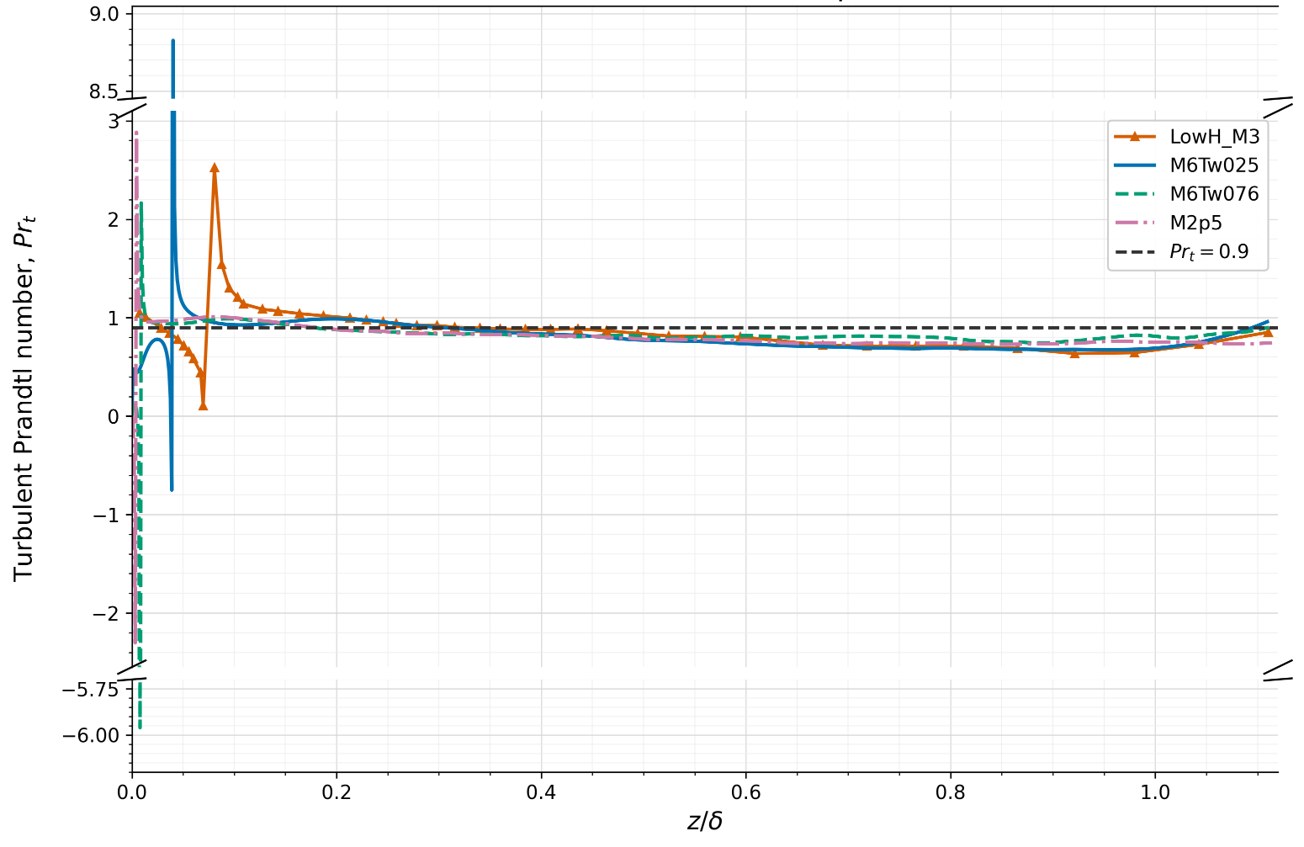
\includegraphics[width=0.8\linewidth]{06_Eval_Methodology/06_Figures/Turb_Prandtl_Number_Comparison.png}
    \caption[DNS turbulent-Prandtl-number distributions]{Turbulent Prandtl number across the whole boundary layer height, with wall-normal distance \(z\) normalized by the respective boundary layer thickness \(\delta\). M2p5, M6Tw025 and M6Tw076 use Zhang et al.'s DNS data~\cite{zhang2018direct}; LowH\_M3 uses the digitized Martin--Duan Part~4 distribution~\cite{duan2011direct_Part4}. The dashed horizontal line marks the RANS value \(Pr_t=0.9\). Breaks in the vertical axis retain the large excursions near the wall while exposing the order-unity variation over the rest of the profile. The M2p5 and M6Tw076 are adiabatic cases, whereas LowH\_M3 and M6Tw025 are strongly cold-wall cases (see Section~\ref{sec:evaluation:benchmark-cases}).}
    \label{fig:evaluation:turb_prandtl_comparison}
\end{figure}

The RANS \(Pr_t\)sensitivity calculations represented in Figure~\ref{fig:evaluation:turb_prandtl_comparison_thermal_profile} provides further evidence that the thermal closure materially affects the \(T(U)\) profile. Reducing the constant \(Pr_t\) from \(1.0\) to \(0.6\) lowers the predicted temperature maximum in both models and brings it closer to DNS. No displayed constant reproduces the entire relation: the curves retain differences on the upper,  recovering region. This aligns with the previous observation that the M6Tw025 case has a near-wall \(Pr_t\) distribution that remains below unity over a broader part of the inner boundary layer.

\begin{figure}[H]
    \centering
    % Figure provenance and typography restoration (2026-10-19):
    %   Original high-resolution export: ../Weekly 260803.pptx, slide 21,
    %     archive member ppt/media/image13.png (3189 x 1232 pixels).
    %   Retained source and reproduction script:
    %     thesis/06_Eval_Methodology/06_Figures/thermal_BL_profile_Prt_source/
    %     original_export.png, restore_typography.py and provenance.json.
    %   Original sensitivity-study data/script were not located. Curve pixels
    %     are preserved; axes/ticks/legends are replaced with larger vector text.
    %     This restores typography rather than replotting numerical data.
    % End figure provenance.
    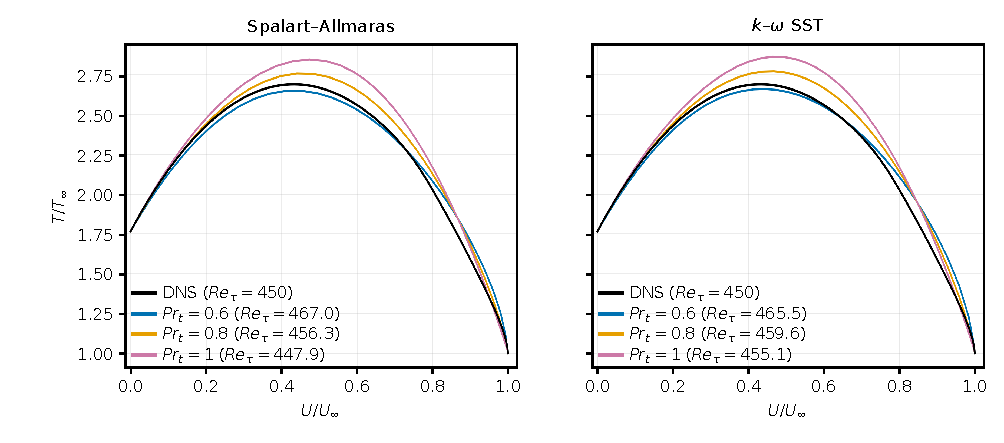
\includegraphics[width=\linewidth]{06_Eval_Methodology/06_Figures/thermal_BL_profile_Prt.pdf}
    \caption[Effect of constant \(Pr_t\) on the M6Tw025 temperature--velocity relation]{Sensitivity of the M6Tw025 mean temperature--velocity relation to constant \(Pr_t=0.6\), \(0.8\) and \(1.0\) in wall-resolved SA (left) and \(k\)--\(\omega\) SST (right). Temperature and velocity are normalized by the freestream values. The DNS reference has \(Re_\tau=450\); the RANS stations have approximately \(448\leq Re_\tau\leq467\), as listed in the legends. These stations differ from the \(Re_{\delta2}\)-matched baseline protocol. Lower \(Pr_t\) reduces the thermal maximum but does not remove the discrepancy over the complete relation.}
    \label{fig:evaluation:turb_prandtl_comparison_thermal_profile}
\end{figure}

Taken together, the DNS distributions, the similar thermal-profile errors of two different momentum closures, and the constant-\(Pr_t\) sensitivity identify the thermal closure as a plausible contributor to the discrepancies. They do not isolate it from errors in the eddy viscosity or from other modelling assumptions. Related hypersonic calculations by Huang et al. found improved temperature predictions with an algebraic turbulent-energy-flux closure compared with constant \(Pr_t\), using an algebraic momentum model~\cite{huang2020simulation}. That result supports further investigation of the thermal closure, while its different momentum model prevents direct attribution of the present SA and SST errors to \(Pr_t\) alone.
\par\medskip

\subsection{Assessment of results and comparison to existing publications}
\label{subsec:comparative:zpg:results-assessment}

Several published RANS assessments use the Zhang and Huang benchmarks included in Table~\ref{tab:evaluation:selected-cases}. They provide context for the wall-load errors and thermal-profile discrepancies found here, but common case and model names do not ensure equivalent calculations. The following comparison identifies differences in model formulation, mean-flow coupling, inflow conditions and sampling location that affect interpretation of Table~\ref{tab:wall-resolved:coefficients}.

\paragraph*{Huang et al. (2019)}

Huang et al.~\cite{huang2019assessment} assess SA and SST for M8Tw048 and report wall-coefficient errors within \(5\%\), broadly consistent with the small errors obtained here for this case. Their calculations use \(Pr_t=0.85\) and \(Re_\tau\) matching, whereas the present baseline uses \(Pr_t=0.9\) and \(Re_{\delta2}\) matching (Section~\ref{subsec:evaluation:matching-station}). Moreover, reconstructing the DNS heat-flux from the published, rounded \(-B_q\) introduces a \(\pm8.33\%\) rounding bound (Table~\ref{tab:evaluation:zhang-bq-rounding}). This limits comparisons based on that reconstruction and it is not an uncertainty estimate for Huang et al.'s underlying DNS data.

\paragraph*{Aiken et al. (2022)}

Aiken et al.~\cite{aiken2022assessment} assess SA, \(k\)--\(\omega\) BSL and SST against six Zhang and Huang benchmarks at \(Pr_t=0.9\). They report thermal-profile discrepancies similar to those in Section~\ref{subsec:comparative:zpg:wr-profiles} and identify the thermal closure as a possible contributor. Their tested freestream-turbulence variations have little downstream influence for M8Tw048. However, their SA model includes the Catris--Aupoix correction, distinct from the implementation correction in Section~\ref{subsec:ext:spalart-allmaras-of-correction}, and their original SST formulation differs from the updated version described in Section~\ref{sec:background:rans-turbulence-modelling}. They match \(Re_\tau\), while reporting similar errors with \(Re_\theta\) matching. Their Table~1 also lists total enthalpies inconsistent with the stated flow conditions, and Table~3 contains inconsistent \(Re_\theta/\theta\) values for M8Tw048. These reporting issues limit reproducibility without establishing that the imposed flow states were incorrect. Together with the formulation differences, they prevent treating agreement or disagreement as a direct code-verification result, consistent with the reporting concerns of Viti et al.~\cite{viti2007numerical}.

\paragraph*{Danis (2023)}

Danis~\cite[Figure~4.10]{danis2023direct} compares original SST skin-friction predictions with DNS for M6Tw025, M14Tw018 and M11Tw020 as functions of \(Re_\tau\), without a corresponding SST wall-heat-flux comparison. The calculations use VULCAN-CFD and cite Menter's 1994 SST model, but the turbulent Prandtl number and detailed model settings are not specified in that assessment. Differences from the present skin-friction results therefore cannot be attributed to a particular modelling or implementation choice.

\paragraph*{Vaughan et al. (2025)}

Vaughan et al.~\cite{vaughan2025paper} and Vaughan's master's thesis~\cite{vaughan2025thesis} examine overlapping Zhang and Huang cases. The thesis likewise finds cold-wall thermal-profile discrepancies at \(Pr_t=0.9\), but uses SA-neg and a vorticity-based SST limiter, rather than the present model variants. It selects sampling locations by matching the initial DNS boundary layer thickness and then advancing by the reported downstream distance, rather than matching \(Re_\tau\). This is the shifted-station approach discussed in Section~\ref{subsec:evaluation:matching-station}.
\par\medskip

For SST, Vaughan's documented mean-flow equations retain the isotropic turbulent stress, turbulent kinetic energy in total energy, and its diffusive transport, whereas the present HiSA formulation omits these contributions. Zhang et al.~\cite{zhang2021formulation} found sensitivity to these terms in shock interactions but little influence on skin-friction and velocity profiles for their single Mach-5 flat-plate. That result does not establish negligible heating sensitivity for the present cases.
\par\medskip

Vaughan also interprets the DNS freestream states as post-shock values and supplies modified pre-shock inflows~\cite[Tables~2.2--2.3]{vaughan2025thesis}. The reconstruction procedure is unspecified and a discrepancy arises for M14Tw018, where the tabulated pre-shock mean-flow total enthalpy \(c_pT+U^2/2\) exceeds the DNS value by \(4.56\%\). Table~\ref{tab:inflow-comparison} tests these inflows in the present SST implementation for four Zhang cases, retaining each run's own \(Re_{\delta2}\)-matched station. This demonstrates sensitivity to the inflow specification, but neither establishes which inflow better reproduces DNS nor reproduces Vaughan's complete setup.

% Data: /home/mgnadlinger/Zhang_DNS_ZPGFP/kwSST_Prt0p9/inflow_comparison_20261017/comparison_native_with_DNS.csv
% Extraction: add_dns_reference.py --matching native in the same directory;
% station and DNS-reference provenance: DNS_reference_native_audit.json.
\begin{table}[H]
    \centering
    \caption[Inflow sensitivity of wall-resolved SST wall loads]{Inflow sensitivity of the present wall-resolved \(k\)--\(\omega\) SST simulations against Zhang's DNS~\cite{zhang2018direct}. Original inflows use the DNS freestream conditions in Table~\ref{tab:evaluation:zhang-inflow-wall}; modified inflows use Vaughan's pre-shock values~\cite[Table~2.2]{vaughan2025thesis}. Each run is evaluated at its own \(Re_{\delta2}\)-matched station using its respective inlet density and velocity. Parentheses give \(100(\mathrm{RANS}-\mathrm{DNS})/\mathrm{DNS}\). Heat-flux is positive into the wall; shear stress is its magnitude. The M6Tw076 heat-flux reference is nominal and retained only for this sensitivity comparison, subject to the rounding and wall-temperature limitations in Section~\ref{sec:evaluation:benchmark-cases}.}
    \label{tab:inflow-comparison}
    \small
    \begin{tabular}{@{}llrr@{}}
        \toprule
        Case & Reference / inflow & \(q_w\) [\(\mathrm{kW\,m^{-2}}\)] & \(\tau_w\) [\(\mathrm{Pa}\)] \\
        \midrule
        M6Tw025 & \textbf{Zhang DNS} & \textbf{11.4888} & \textbf{28.3210} \\
        M6Tw025 & Original & 11.8290 (\(+2.96\%\)) & 29.2326 (\(+3.22\%\)) \\
        M6Tw025 & Vaughan & 11.4180 (\(-0.62\%\)) & 28.2175 (\(-0.37\%\)) \\
        \addlinespace
        M6Tw076 & \textbf{Zhang DNS} & \textbf{2.1720} & \textbf{16.2533} \\
        M6Tw076 & Original & 1.8925 (\(-12.87\%\)) & 15.3712 (\(-5.43\%\)) \\
        M6Tw076 & Vaughan & 1.8585 (\(-14.43\%\)) & 15.1801 (\(-6.60\%\)) \\
        \addlinespace
        M8Tw048 & \textbf{Zhang DNS} & \textbf{4.5495} & \textbf{13.2915} \\
        M8Tw048 & Original & 4.6231 (\(+1.62\%\)) & 13.3289 (\(+0.28\%\)) \\
        M8Tw048 & Vaughan & 4.5881 (\(+0.85\%\)) & 13.2067 (\(-0.64\%\)) \\
        \addlinespace
        M14Tw018 & \textbf{Zhang DNS} & \textbf{10.3028} & \textbf{12.1640} \\
        M14Tw018 & Original & 11.7582 (\(+14.13\%\)) & 14.0633 (\(+15.61\%\)) \\
        M14Tw018 & Vaughan\textsuperscript{*} & 12.3612 (\(+19.98\%\)) & 14.3311 (\(+17.82\%\)) \\
        \bottomrule
    \end{tabular}
    \par\smallskip
    \begin{minipage}{\linewidth}
        \footnotesize
        \textsuperscript{*} Vaughan's tabulated M14Tw018 pre-shock mean-flow total enthalpy \(c_pT+U^2/2\) is \(4.56\%\) higher than that of the DNS freestream state.
    \end{minipage}
\end{table}

\paragraph*{Cheng et al. (2026)}

Cheng et al.~\cite{cheng2026reynolds} use OpenFOAM-v2312 and the HiSA solver framework to investigate energy closures with the Durbin--Yin \(k\)--\(\omega_0\) model, including additional SST--\(\omega_0\) tests. Their baseline therefore differs from the present SST model even before the proposed energy-closure corrections. Their stated energy equation includes turbulent-kinetic-energy transport~\cite[Eq.~2.7]{cheng2026reynolds}, which is absent from the present HiSA formulation. The paper does not specifically state having performed the corresponding solver modifications outside of the stated RANS equations. Shared solver ancestry consequently does not establish equivalent mean-flow coupling. Station selection adds another difference, although the present tests in Tables~\ref{tab:evaluation:matching-station-bq} and~\ref{tab:evaluation:matching-station-ch} give changes below \(1\%\) in \(-B_q\) and \(2\%\) in \(C_h\) between the shifted and \(Re_{\delta2}\)-matched stations. Their Table~5 also normalizes \(B_q\) with DNS wall quantities, whereas Table~\ref{tab:wall-resolved:coefficients} uses each solution's own wall state. These values require consistent normalization before comparison.

\paragraph*{Implications for the present assessment}

The literature supports treating the present discrepancies as part of a broader difficulty in predicting cold-wall boundary layers with conventional RANS closures. It does not provide an equivalent setup for direct code verification or isolate the cause of differences in wall loads. In particular, the thermal-profile deficiencies reported by Aiken and Vaughan reinforce the evidence in Sections~\ref{subsec:comparative:zpg:wr-profiles} and~\ref{subsec:comparative:zpg:wr-prandtl}, without establishing constant \(Pr_t\) as their sole cause. The subsequent wall-function assessment therefore retains both DNS and the present wall-resolved SA solution as distinct references, as defined in Table~\ref{tab:erriso:reference-hierarchy}.

\subsection{Selection of cases for detailed wall-function assessment}
\label{subsec:comparative:zpg:case-selection}

M6Tw025 and LowH\_M3 are retained for the detailed coupled wall-function analysis because they expose different relationships between wall-coefficient and profile accuracy. M6Tw025 supplies digital DNS profiles for a strongly cooled Mach-6 boundary layer and exhibits a clear thermal-profile discrepancy in both RANS models. It therefore tests the wall functions when their analytical thermal relation is coupled to a resolved RANS field that already differs from DNS. Its detailed reference profiles also permit an independent prescribed-profile closure assessment, subject to the heat-flux reporting limitations stated above.
\par\medskip

LowH\_M3 supplies a cold-wall supersonic comparison in which the resolved RANS \(T(U)\) relation closely follows the digitized DNS. This reduces the pronounced thermal-profile mismatch present in M6Tw025 and makes the case useful for examining additional errors introduced by the wall function and the CFD mesh. The nonzero wall-coefficient errors remain part of its baseline. In the subsequent prescribed-profile calculations, the resolved SA field is used as the LowH\_M3 input, so those closure errors measure consistency with SA rather than an independent reconstruction of DNS wall quantities.
\par\medskip

The contrasting thermal-profile accuracy of LowH\_M3 and M6Tw025 cannot be attributed to the models' incompressible origins alone. The corresponding DNS studies~\cite{zhang2018direct,duan2011direct_Part4} report approximate Morkovin-type similarity and outer-layer agreement with modified strong Reynolds analogies for both cases (ref. Section \ref{subsec:background:SRA-Morkovin}). This weakens an explanation based on a fundamental loss of applicability between the two flow conditions, without excluding differences in intrinsic compressibility, mean-property gradients or thermal transport. The cause of the contrast remains unresolved, with the following analysis therefore examining the shared constant turbulent Prandtl number as a possible contributor.

\section{Wall-function closure assessment}
\label{sec:comparative:zpg:cross-comparison}

The previous wall-resolved assessment established the discrepancy of the underlying RANS calculation from DNS. Adding a wall function to a RANS simulation introduces a further relationship between the sampled flow state and the resulting wall shear stress and heat-flux. To examine that relationship separately, the analytical closures are now evaluated on prescribed boundary layer profiles. This a-priori assessment asks how well a closure can recover the known wall heat-flux and shear stress, when its off-wall sampled inputs are ideal, i.e. supplied from the respectilve known reference boundary layer profile. It provides the comparison needed to distinguish a wall function's underlying closure behaviour from the additional changes that occur when the same wall function is coupled to full FVM CFD simulation.
\par\medskip

The detailed discussion focuses on M6Tw025 and LowH\_M3, which also carry the comparison into the subsequent coupled CFD assessment (as established in Section~\ref{subsec:comparative:zpg:case-selection}). The initial M6Tw025 sweeps use the digitally published DNS profiles and wall quantities of Zhang et al.~\cite{zhang2018direct}. LowH\_M3 lacks similar high quality published DNS reference data, so it uses the wall-resolved SA profile and its corresponding wall quantities at the matched comparison station (Section~\ref{subsec:evaluation:matching-station}) are used. For LowH\_M3, the reported closure errors are thus relative to the wall-resolved SA wall quantities. An additional M6Tw025 comparison in Section~\ref{subsec:erriso:rans-profile-influence} applies the same Li closure to DNS and resolved SA inputs to assess the influence of the supplied profile. Results for the additional cases are collected in Appendix~\ref{app:zpg:apriori}.

\subsection{A-priori inverse solution}
\label{subsec:erriso:apriori-solver}

For an a-priori assessment, a virtual sampling point is moved through a known, resolved boundary layer profile. At every sampling height, the required velocity and thermodynamic state are interpolated from that given profile and supplied to the wall-function closure equations, together with the required physical wall temperature and transport properties. The wall heat-flux and shear stress are then recovered by an inverse solution of the closure equations. The reference friction velocity defines the sampling coordinate,
\begin{equation}
    y_{\mathrm{ref}}^+
    = \frac{\rho_{w,\mathrm{ref}}u_{\tau,\mathrm{ref}}y}
    {\mu_{w,\mathrm{ref}}},
    \qquad
    u_{\tau,\mathrm{ref}}
    = \sqrt{\frac{\tau_{w,\mathrm{ref}}}{\rho_{w,\mathrm{ref}}}}.
\end{equation}

For the Li formulation, introduced in Section~\ref{subsec:wall-functions:gao-li:governing-relations}, the first-point velocity and enthalpy, the physical wall state, and an arbitrarily placed second reference state determine the generalized enthalpy--velocity relation. Two reference choices are examined. The two-point construction assumes two virtual cells of equal height, so their centres satisfy \(y_2=3y_1\). Both point states are interpolated from the resolved profile. In the alternative construction, the reference state is prescribed at the boundary layer edge. Li et al propses the former, two-point construction, so that the wall function closures are independant of the boundary layer edge quantities \cite{li2025WF}, for comparison and evaluation the latter, boundary layer edge construction was selected to be included in the analysis. In either case, the unified velocity law is inverted for \(u_\tau\), and the wall outputs follow from \(\tau_w=\rho_wu_\tau^2\) and the wall function's heat-flux relation.
\par\medskip

For the Griffin formulation, introduced in Section~\ref{subsec:wall-functions:griffin:governing-relations}, the sampled velocity and thermodynamic state are combined with the wall temperature and boundary layer-edge quantities - Griffin et al do not propose a specific approach to allow for a two-point, boundary layer edge free construction. For each sample point, the inverse-transformation model is integrated from the wall region to the sample point. The wall stress is iterated until the integrated velocity reproduces the prescribed matching point's velocity. The temperature--velocity relation then supplies the wall heat-flux. The prescribed wall stress and heat-flux of the reference profile are used to assess the recovered outputs, rather than imposed as their solution targets.
\par\medskip

Edge states are supplied according to the available reference data. Griffin uses the supplied \(\delta_{99}\) for the Zhang DNS profiles and its edge criterion for LowH\_M3, whereas the prescribed-edge Li comparison for LowH\_M3 uses the \(U=0.99U_\infty\) crossing.
\par\medskip

The reported errors in this section are signed relative differences,
\begin{equation}
    \varepsilon_X
    = 100\left(\frac{X_{\mathrm{closure}}}{X_{\mathrm{ref}}}-1\right),
    \qquad X\in\{\tau_w,q_w\}.
    \label{eq:erriso:apriori-relative-error}
\end{equation}

The reference being either the DNS wall quantities or the wall-resolved RANS quantities, depending on the profile being sampled. The a-priori assessment is therefore a standalone evaluation of the closure's ability to recover the known wall fluxes from known inputs, and thus evaluates the wall function's closure theories in isolation.

\paragraph*{Consistency with the published Griffin assessment}
An independent check of the herin implemented a-priori solver on the Griffin evaluation is available from the a-priori results of Griffin et al.~\cite[Figure~5]{griffin2023WF}. Their matching height is \(y_m=0.3\delta_{99}\). In reference wall units, this corresponds to \(y_m^+=0.3\mathrm{Re}_\tau\). Table~\ref{tab:erriso:Griffin-a-priori-validation} compares the present inverse solutions at those heights with the errors read from the published figure for two identifiable Zhang cases.

\begin{table}[H]
    \centering
    \caption[Consistency check of the Griffin a-priori solver]{Comparison of the present Griffin a-priori solver at \(y_m=0.3\delta_{99}\) with Griffin et al.~\cite[Figure~5]{griffin2023WF}. Published errors are approximate values read from the figure; the comparison checks consistency of the standalone closure evaluation.}
    \label{tab:erriso:Griffin-a-priori-validation}
    \begin{tabular}{@{}l
        S[table-format=3.3]
        S[table-format=\approx-2]
        S[table-format=-2.2]
        S[table-format=\approx-2]
        S[table-format=-2.2]@{}}
        \toprule
        & & \multicolumn{2}{c}{\(\tau_w\) error [\%]} & \multicolumn{2}{c}{\(q_w\) error [\%]} \\
        \cmidrule(lr){3-4}\cmidrule(l){5-6}
        Case & {\(y_m^+\)} & {Griffin et al.} & {Present solver} & {Griffin et al.} & {Present solver} \\
        \midrule
        M6Tw025  & 134.561 & \approx -13 & -11.56 & \approx -15 & -15.28 \\
        M14Tw018 & 192.588 & \approx -10 & -11.32 & \approx -15 & -15.91 \\
        \bottomrule
    \end{tabular}
\end{table}

The present solutions reproduce the sign and approximate magnitude of the published errors to within the uncertainties of the published graph's resolution. Their agreement supports the use of the a-priori solver used in the following to examine matching-height sensitivity of the closure theories.

\subsection{Closure errors versus sampling height}
\label{subsec:erriso:apriori-results}

Figures~\ref{fig:wall-closure:a-priori-Li-M6Tw025}--\ref{fig:wall-closure:a-priori-Griffin-LowHM3} assess the closures by Li and Griffin jointly on the M6Tw025 DNS profile and the LowH\_M3 wall-resolved SA profile. Both formulations recover the wall quantities with significant errors over the varying sampling height, but neither is notably more accurate than the other. But it shows, that the Li's two-reference-point method, rather than relying on boundary layer edge quantities, works without a systematic loss of accuracy (e.g. see Figure~\ref{fig:wall-closure:a-priori-Li-M6Tw025} dashed vs. solid line). And it should be note that both Li and Griffin's formulations don't show significantly higher errors in the buffer layer, highlighting that the blending between the sublayer and law-of-the-wall for these adaptive wall functions work well and doesn't present a \(y^+\) meshing region to be specifically avoided.
\par\medskip

Across all the investigated profiles (including the cases in Appendix~\ref{app:zpg:apriori}) Griffin gives signed shear-stress errors of approximately \(-11\%\) to \(+11\%\) and heat-flux errors of \(-14\%\) to \(+6\%\), over the reasonable range of \(1\le y_{\mathrm{ref}}^+\le100\). Over the same cases and sampling-height interval, the Li closure gives respective shear-stress errors of approximately \(-7\%\) to \(+13\%\) and heat-flux errors of \(-15\%\) to \(+18\%\). These are appreciable closure errors for prescribed, ideal, inputs and warrant ongoing research into finding better velocity transformation like by Hasan et al.\cite{hasan2023incorporating} and improved closure formulations.
\par\medskip

The heat-flux ranges exclude M2p5, whose adiabatic reference makes relative heat-flux errors undefined, and M6Tw076, owing to the reference-data limitations described in Section~\ref{sec:evaluation:benchmark-cases}.
\par\medskip

At the largest sampling height, Li's prescribed-edge M6Tw025 heat-flux error rises to approximately \(+79\%\) at \(y_1^+=400\), with a reported \(Re_\tau = 450\) \cite{zhang2018direct}, this corresponds to a sampling station at about \(0.89\delta_{99}\). Li's two-reference point method, is not applicable anymore at these sampling stations because the second reference point sits outside of the boundary layer, this is a limit of this method. The high error at these high sampling points, is consistent with increasing sensitivity of the enthalpy inversion as the sampled and reference velocities approach one another, especially because the first sampling point also lies outside the inner layer~\cite[Eq.~(40)]{li2025WF}. Griffin avoids this particular inversion sensitivity by prescribing the wall temperature--velocity slope through its Reynolds analogy. It shows significant improvement to this high \(y^+\) sensitivity, but does not establish universal validity near the boundary layer edge. The published a-priori comparison uses \(y_m=0.3\delta_{99}\); the additional WMLES matching-height studies discussed in Section~\ref{subsec:wall-functions:griffin:validation-scope} do not extend this assessment towards the edge.

\clearpage

\begin{figure}[H]
    \centering
    % Figure provenance (WSL; absolute paths):
    %   Figure: /home/mgnadlinger/OpenFOAM/mgnadlinger-v2412/src/LiWallFunctions/tests/ReverseSolver/M6Tw025_Stat_Zhang/wall_flux_errors_vs_yplus.png
    %   Python scripts:
    %     /home/mgnadlinger/OpenFOAM/mgnadlinger-v2412/src/LiWallFunctions/tests/ReverseSolver/plot_m6tw025_flux_reference_overlay.py
    %     /home/mgnadlinger/OpenFOAM/mgnadlinger-v2412/src/LiWallFunctions/tests/ReverseSolver/analyze_li_wall_function_profile_Zhang.py
    %   Data / simulation roots (high-level):
    %     /home/mgnadlinger/OpenFOAM/mgnadlinger-v2412/src/LiWallFunctions/tests/ReverseSolver/M6Tw025_Stat_Zhang
    %     /home/mgnadlinger/OpenFOAM/mgnadlinger-v2412/src/LiWallFunctions/tests/ReverseSolver/M6Tw025_Stat_Zhang_boundaryLayerEdge
    %     /home/mgnadlinger/OpenFOAM/mgnadlinger-v2412/src/LiWallFunctions/tests/ReverseSolver
    %     /home/mgnadlinger/Zhang_DNS_ZPGFP/References/Data
    %   Note: The plot combines the second-cell and boundary-layer-edge a-priori sweep directories.
    %   Note: The staged DNS input in ReverseSolver includes added Cf/Ch header fields; its DNS profile rows
    %     match References/Data.
    %   Thesis replot: Figures/Closures/plot_apriori_assessments.py; byte-for-byte
    %     saved sweeps and original paths/hashes in Figures/Closures/apriori_sources/.
    %   Layout: shear left, heat flux right; original 10.5 pt plot font retained.
    % End figure provenance.
    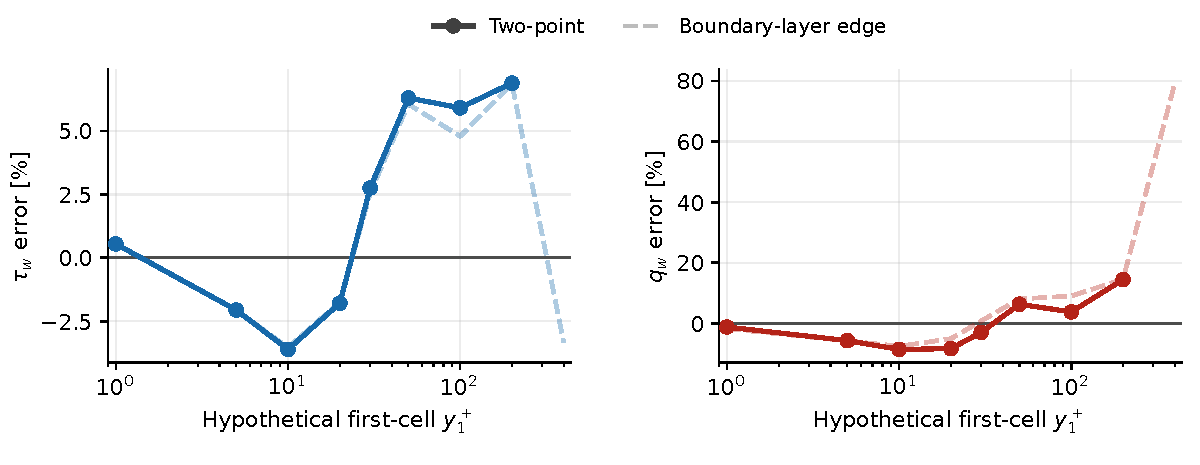
\includegraphics[width=\linewidth]{07_Error_Isolation_Results/Figures/Closures/a-priori_Li_M6Tw025.pdf}
    \caption[Li closure assessment on the M6Tw025 DNS profile]{A-priori Li wall-shear (left) and heat-flux (right) errors relative to the M6Tw025 DNS wall quantities. The solid curves use two virtual equal-height cells, with \(y_2=3y_1\); the dashed curves use a prescribed boundary layer-edge state. The horizontal coordinate is the virtual first-cell-centre height in DNS wall units. Each point is a separate inverse closure solution on the same prescribed profile.}
    \label{fig:wall-closure:a-priori-Li-M6Tw025}
\end{figure}

\begin{figure}[H]
    \centering
    % Figure provenance (WSL; absolute paths):
    %   Figure: /home/mgnadlinger/OpenFOAM/mgnadlinger-v2412/src/GriffinWallFunctions/tests/ReverseSolver/M6Tw025_Stat_Zhang/wall_flux_errors_vs_yplus.png
    %   Python script:
    %     /home/mgnadlinger/OpenFOAM/mgnadlinger-v2412/src/GriffinWallFunctions/tests/ReverseSolver/analyze_griffin_wall_function_profile_Zhang.py
    %   Data / simulation roots (high-level):
    %     /home/mgnadlinger/OpenFOAM/mgnadlinger-v2412/src/GriffinWallFunctions/tests/ReverseSolver/M6Tw025_Stat_Zhang
    %     /home/mgnadlinger/OpenFOAM/mgnadlinger-v2412/src/GriffinWallFunctions/tests/ReverseSolver
    %     /home/mgnadlinger/Zhang_DNS_ZPGFP/References/Data
    %   Note: The staged DNS input in ReverseSolver includes added Cf/Ch header fields; its DNS profile rows
    %     match References/Data.
    %   Thesis replot: Figures/Closures/plot_apriori_assessments.py; byte-for-byte
    %     saved sweeps and original paths/hashes in Figures/Closures/apriori_sources/.
    %   Layout: shear left, heat flux right; original 10.5 pt plot font retained.
    % End figure provenance.
    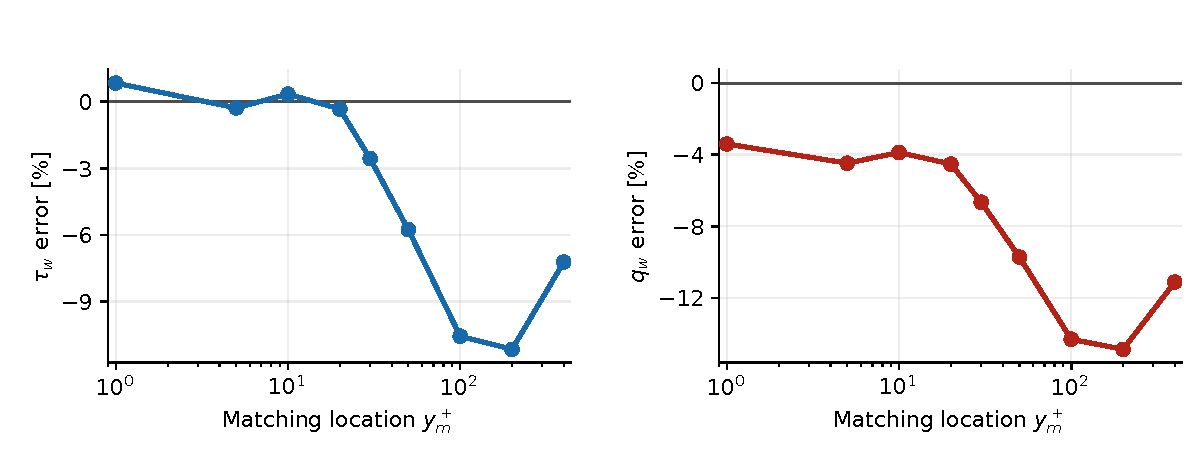
\includegraphics[width=\linewidth]{07_Error_Isolation_Results/Figures/Closures/a-priori_Griffin_M6Tw025.pdf}
    \caption[Griffin closure assessment on the M6Tw025 DNS profile]{A-priori Griffin wall-shear (left) and heat-flux (right) errors relative to the M6Tw025 DNS wall quantities. The prescribed DNS edge state remains fixed while the virtual matching height \(y_m^+\) is varied. Points above \(y_m=0.3\delta_{99}\), corresponding here to \(y_m^+\simeq134.6\), extend the assessment beyond the matching height used in the published a-priori comparison and are retained as sensitivity results.}
    \label{fig:wall-closure:a-priori-Griffin-M6Tw025}
\end{figure}

\clearpage

\begin{figure}[H]
    \centering
    % Figure provenance (WSL; absolute paths):
    %   Figure: /home/mgnadlinger/OpenFOAM/mgnadlinger-v2412/src/LiWallFunctions/tests/ReverseSolver/LowH_M3_Duan_Li/wall_flux_errors_vs_yplus.png
    %   Python scripts:
    %     /home/mgnadlinger/OpenFOAM/mgnadlinger-v2412/src/LiWallFunctions/tests/ReverseSolver/plot_m6tw025_flux_reference_overlay.py
    %     /home/mgnadlinger/OpenFOAM/mgnadlinger-v2412/src/LiWallFunctions/tests/ReverseSolver/analyze_li_wall_function_profile_Duan.py
    %   Data / simulation roots (high-level):
    %     /home/mgnadlinger/OpenFOAM/mgnadlinger-v2412/src/LiWallFunctions/tests/ReverseSolver/LowH_M3_Duan_Li
    %     /home/mgnadlinger/OpenFOAM/mgnadlinger-v2412/src/LiWallFunctions/tests/ReverseSolver/LowH_M3_Duan_Li_boundaryLayerEdge
    %     /home/mgnadlinger/OpenFOAM/mgnadlinger-v2412/src/LiWallFunctions/tests/ReverseSolver/LowH_M3_Duan
    %     /home/mgnadlinger/Duan_DNS_ZPGFP/Martin_Duan_Part4/SA_Prt0p9/LowH_M3
    %   Note: Closure input is the wall-resolved SA profile at time 20000.
    %   Note: The plot combines the second-cell and boundary-layer-edge a-priori sweep directories.
    %   Thesis replot: Figures/Closures/plot_apriori_assessments.py; byte-for-byte
    %     saved sweeps and original paths/hashes in Figures/Closures/apriori_sources/.
    %   Layout: shear left, heat flux right; original 10.5 pt plot font retained.
    % End figure provenance.
    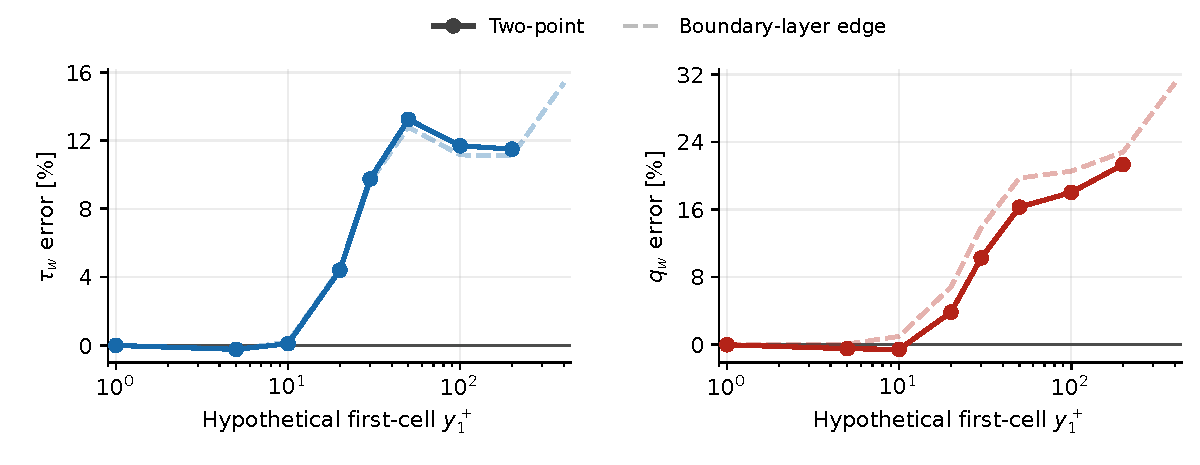
\includegraphics[width=\linewidth]{07_Error_Isolation_Results/Figures/Closures/a-priori_Li_LowHM3.pdf}
    \caption[Li closure assessment on the LowH\_M3 wall-resolved profile]{A-priori Li wall-shear (left) and heat-flux (right) errors relative to the wall-resolved SA baseline for LowH\_M3. Solid curves use the two-point formulation, with \(y_2=3y_1\), and dashed curves use the prescribed \(0.99U_\infty\) edge state. Sampling heights are expressed in wall units of the unchanged SA reference profile. These are closure errors relative to RANS, rather than errors relative to DNS.}
    \label{fig:wall-closure:a-priori-Li-LowHM3}
\end{figure}

\begin{figure}[H]
    \centering
    % Figure provenance (WSL; absolute paths):
    %   Figure: /home/mgnadlinger/OpenFOAM/mgnadlinger-v2412/src/GriffinWallFunctions/tests/ReverseSolver/LowH_M3_Duan/wall_flux_errors_vs_yplus.png
    %   Python script:
    %     /home/mgnadlinger/OpenFOAM/mgnadlinger-v2412/src/GriffinWallFunctions/tests/ReverseSolver/analyze_griffin_wall_function_profile_Duan_Part4.py
    %   Data / simulation roots (high-level):
    %     /home/mgnadlinger/OpenFOAM/mgnadlinger-v2412/src/GriffinWallFunctions/tests/ReverseSolver/LowH_M3_Duan
    %     /home/mgnadlinger/Duan_DNS_ZPGFP/Martin_Duan_Part4/SA_Prt0p9/LowH_M3
    %   Note: Closure input is the wall-resolved SA profile at time 20000.
    %   Thesis replot: Figures/Closures/plot_apriori_assessments.py; byte-for-byte
    %     saved sweeps and original paths/hashes in Figures/Closures/apriori_sources/.
    %   Layout: shear left, heat flux right; original 10.5 pt plot font retained.
    % End figure provenance.
    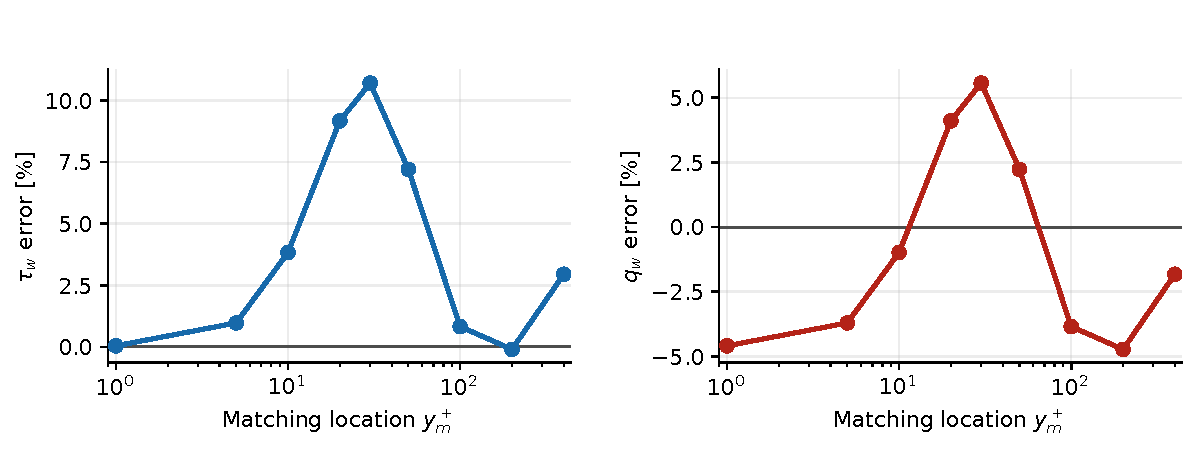
\includegraphics[width=\linewidth]{07_Error_Isolation_Results/Figures/Closures/a-priori_Griffin_LowHM3.pdf}
    \caption[Griffin closure assessment on the LowH\_M3 wall-resolved profile]{A-priori Griffin wall-shear (left) and heat-flux (right) errors relative to the wall-resolved SA baseline for LowH\_M3. The edge state is reconstructed once from the resolved profile using the Griffin boundary layer criterion, then held fixed while the virtual matching height is varied. The point at \(y_m^+=400\) lies above \(0.3\delta_{99}\) of this reconstructed boundary layer and is included as a sensitivity result.}
    \label{fig:wall-closure:a-priori-Griffin-LowHM3}
\end{figure}

\clearpage

\subsection{Influence of the prescribed RANS profile}
\label{subsec:erriso:rans-profile-influence}

In the previous Section\ref{sec:comparative:zpg:wall-resolved-baselines}, with the assessment of turbulence models, the wall-resolved M6Tw025 comparison in Figure~\ref{fig:wall-resolved:M6Tw025_BL_Profile} revealed a clear discrepancy in the temperature maximum and \(T(U)\) relation compared to the DNS reference. To quantify the consequence of this short coming of the turbulence models to the wall function closure that rely on these profiles, the Li et al. closure is evaluated on both the DNS profile and the wall-resolved SA profile at \(Pr_t=0.9\) and subsequently compared.
\par\medskip

Figure~\ref{fig:wall-closure:Li-M6Tw025-profile-influence} expresses both a-priori solved results relative to the same DNS wall quantities. Replacing the DNS profile as input, with the wall-resolved SA profile, changes the heat-flux prediction substantially, while the shear predictions remain much closer. This aligns with the SA velocity profile matching the DNS reference (see Figure~\ref{fig:wall-resolved:M6Tw025_BL_Profile} bottom right), while the \(T(U)\) profile, which feeds the wall function's energy closure, does not (see Figure~\ref{fig:wall-resolved:M6Tw025_BL_Profile} top left). At \(y_{1,\mathrm{DNS}}^+=30\), the predicted heat-flux increases by \(13.4\%\) relative to the DNS-input prediction, but shear changes by only \(0.1\%\). At \(y_{1,\mathrm{DNS}}^+=100\), the heat-flux error relative to DNS rises from \(+3.2\%\) to \(+16.0\%\). Thus, the thermal-profile discrepancy observed in the resolved calculation has a significant counterpart in the wall-function response, even where the velocity profiles appear convincing, and need to be addressed in future improvements of the turbulence models. In a fully coupled turbulence model + wall function CFD run, this error does not isolated as cleanly as in the a-priori solver here, because of the feedback of the wall function's wall quantity prediction into the overall flow field, but the underlying discrepancy still stands.

\begin{figure}[H]
    \centering
    % Figure provenance (WSL; absolute paths):
    %   Original figure: /home/mgnadlinger/OpenFOAM/mgnadlinger-v2412/src/LiWallFunctions/tests/ReverseSolver/M6Tw025_TM_closure_isolation/wall_flux_comparison.png
    %   Analysis script: /home/mgnadlinger/OpenFOAM/mgnadlinger-v2412/src/LiWallFunctions/tests/ReverseSolver/M6Tw025_TM_closure_isolation/run_comparison.py
    %   Saved data: /home/mgnadlinger/OpenFOAM/mgnadlinger-v2412/src/LiWallFunctions/tests/ReverseSolver/M6Tw025_TM_closure_isolation/comparison.csv
    %   Wall references: /home/mgnadlinger/OpenFOAM/mgnadlinger-v2412/src/LiWallFunctions/tests/ReverseSolver/M6Tw025_TM_closure_isolation/reference_states.csv
    %   Original DNS input: /home/mgnadlinger/Zhang_DNS_ZPGFP/References/Data/M6Tw025_Stat.dat
    %   Original SA input: /home/mgnadlinger/Zhang_DNS_ZPGFP/SA_Prt0p9/M6Tw025/postProcessing/TM_ZPGFP/15000/profile_Re_delta2.csv
    %   Thesis export script: thesis/07_Error_Isolation_Results/Figures/Closures/plot_tm_profile_closure.py
    %   Note: The earlier thesis PNG retained only the original figure's middle row,
    %     omitting its legend. Re-exported from saved CSVs with a shared legend;
    %     both panels retain the common DNS denominator and all eight heights.
    %   Note: Fixed omegaH=0.72; each input retains its native wall state.
    %     This is a complete-profile comparison, not a temperature-only swap.
    % End figure provenance.
    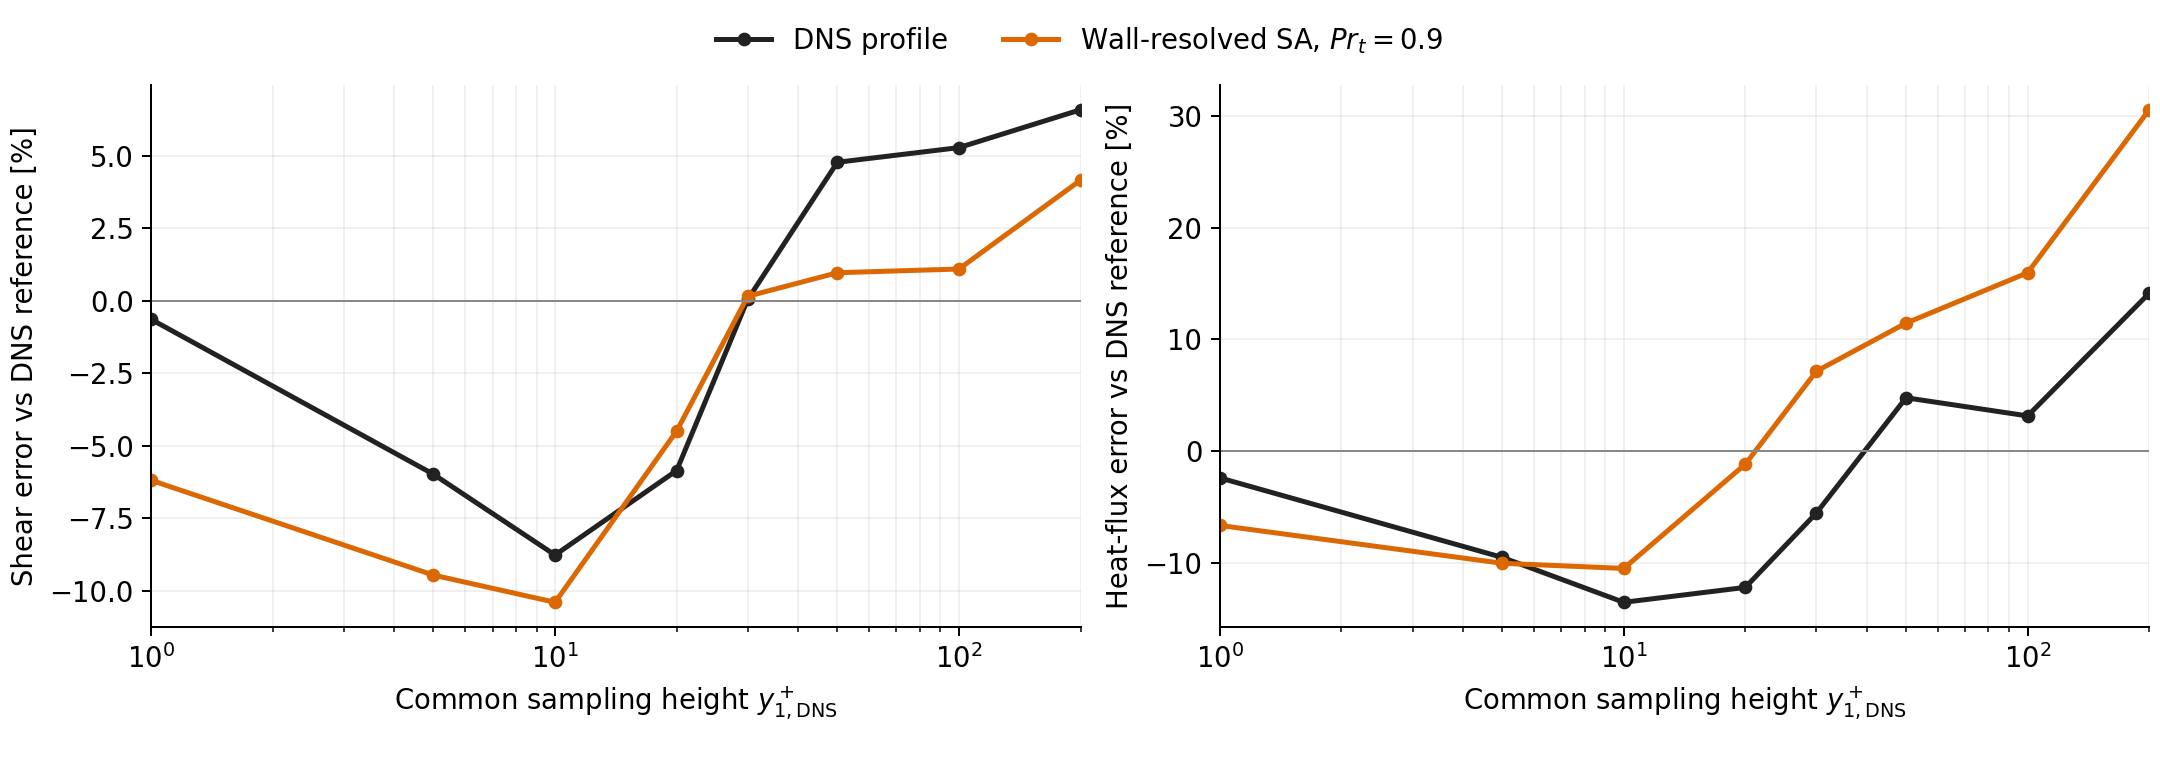
\includegraphics[width=\linewidth]{07_Error_Isolation_Results/Figures/Closures/TM_prof_err_Li-aprio.png}
    \caption[Effect of DNS and SA inputs on the M6Tw025 Li closure]{Li closure evaluated on the M6Tw025 DNS and wall-resolved SA profiles. Left: wall-shear error; right: heat-flux error. Both curves use the DNS wall heat-flux and shear stress as their reference, hence the orange line not converging to zero error at \(y_{1,\mathrm{DNS}}^+=1\). The virtual sampling heights of \(y_1\) and \(y_2=3y_1\) are identical for both inputs; the abscissa uses the supplied DNS wall units.}
    \label{fig:wall-closure:Li-M6Tw025-profile-influence}
\end{figure}

The common DNS denominator in the figure must be distinguished from recovery of each profile's own wall flux. Over e.g. the three sampled heights \(y_{1,\mathrm{DNS}}^+=30\), \(50\) and \(100\), the mean absolute heat-flux error relative to the corresponding source wall value increases from \(4.5\%\) for DNS inputs to \(17.8\%\) for SA inputs. The discrepancy is therefore more than the offset between the resolved SA and DNS wall fluxes itself, hence the discrepancy in the wall-resolved boundary layer to the DNS impacts the wall function closure's accuracy. 
\par\medskip

This is also clearly seen through the immediate mechanism, which is the inferred enthalpy--velocity wall slope in the wall function's energy closure. Li's generalized recovery enthalpy is obtained from
\begin{equation}
    h_{rg}
    =\frac{h_1-h_w(1-r)-h_Rr^2}{r(1-r)},
    \qquad r=\frac{U_1}{U_R},
    \label{eq:erriso:li-reference-inversion}
\end{equation}
where \((U_R,h_R)\) is the reference state, here the second sampling point~\cite[Eq.~(40)]{li2025WF}.

With positive heat-transfer into the cooled wall denoted by \(Q_w=|q_w|\), Li's relations give
\begin{equation}
    S=\left.\frac{\mathrm{d}h}{\mathrm{d}U}\right|_w
      =\frac{h_{rg}-h_w}{U_2},
    \qquad Q_w=\frac{\tau_w S}{Pr_w},
    \label{eq:erriso:li-profile-wall-slope}
\end{equation}
where \(h_{rg}\) follows from Equation~\eqref{eq:erriso:li-reference-inversion}~\cite[Eqs.~(40)--(41)]{li2025WF}. At \(y_{1,\mathrm{DNS}}^+=30\), changing from DNS to SA inputs raises \(S\) by \(13.3\%\), accounting for almost all of the heat-flux increase while the recovered shear is nearly unchanged because so is the sampled velocity profile. This identifies the thermal wall slope as the immediate route through which the profile mismatch affects the predicted heating. Thus future improvements to RANS turbulence models should not only improve the heat-flux and shear stress results in isolation, but also need to tackle the challenge in hypersonic cold-wall boundary layer reproducibility. 

\subsection{Summary and Implications for the coupled assessment}
The a-priori assessment (ref. Section~\ref{subsec:erriso:apriori-results}) identifies appreciable baseline errors in both closures, even when the sampled inputs are supplied from known reference profiles. However, neither formulation shows a systematic breakdown in the buffer layer. The results therefore provide no basis for excluding a buffer-layer sampling interval because of the blending between the viscous and logarithmic relations. But the remaining closure errors do warrant investigation into better, improved velocity transformations and closure theories.
\par\medskip

A comparison of supplying the a-priori solver with the DNS or the wall-resolved SA profile (ref. Section~\ref{subsec:erriso:rans-profile-influence}) identifies a further limitation: discrepancies in the wall-resolved RANS profile (as identified in Section~\ref{subsec:comparative:zpg:wr-profiles}) can substantially alter the wall-function heat-flux prediction. In the example of the Li assessment on the M6Tw025 case, it shows that a convincing velocity profile does not compensate for an inaccurate \(T(U)\) relation, which changes the inferred thermal wall slope. Improving the coupled prediction therefore requires attention to both the closure's baseline accuracy and the turbulence model's reproduction of the cold-wall thermal profile. These findings provide the context for the following assessment of the additional influence of spatial discretization in Section~\ref{subsec:comparative:zpg:yplus-sensitivity}, especially with the final isolation from the closure error by overwriting the closure theory with a fitted function in Section~\ref{subsec:comparative:zpg:fitted-closure}.

\section{Wall-function in FVM CFD: Spatial-discretization error and sampling sensitivity}
\label{subsec:comparative:zpg:yplus-sensitivity}

The closure assessment in Section~\ref{sec:comparative:zpg:cross-comparison} determines how accurately a wall function recovers wall loads from a prescribed, ideal, boundary layer state. In CFD, that state is itself part of a discrete solution. Consequently, a change in sampling height can alter both the closure response and the numerical solution of the surrounding boundary layer. This section analysis the behaviour of the wall functions on the LowH\_M3 and M6Tw025 cases, by first examining their accuracy and consistency on a conventional mesh strategy as the wall functions were intended to be used e.g. by Li et al. in \cite{li2025WF}. Subsequently, a novel boundary layer-informed mesh design is introduced to isolate the identified internal-face discretization errors. Finally the, in the previous section identified, closure discrepancies are revisited in the context of the new meshes, by presccribing an ideally fitted closure to isolate out all found error effects, but from the turbulence models.

\subsection{Wall functions on conventional meshes}
\label{subsec:comparative:zpg:conventional-mesh}

The conventional mesh strategy and sampling geometry are introduced in Section~\ref{subsec:wall-functions:sampling-geometry}. The general idea how conventionally meshes for wall-functions are designed is, to increase the first-cell height until the desired \(y^+_1\) is achieved. In these \textit{conventional wall-function mesh} sweeps, increasing the physical first-cell height moves the wall-function sample outward and increases the separation of neighbouring cell centres. Thus, on \textit{conventional wall-function mesh} the sampling location $y_s^+$ coincides with the first-cell location $y_1^+$, while the spacing of internal-face stencils, herin referred to as \(h^+\),  changes with it (see Figure~\ref{fig:WF:exemplaray_y+10_mesh} \(h^+\) change between exemplary \(y^+_1 = 10\) and \(y^+_1 = 30\) meshes). One should keep in mind, that the sample height $y_s^+$ and physical first-cell mesh resolution \(y^+_1\) need not necessarily be identical, but one could also take the second off-wall cell centre as the wall function sampling point. This distinction becomes essential when the two are varied independently below.
\par\medskip

Figure~\ref{fig:WF:mesh} shows a representative conventional M6Tw025 mesh with special attention to the leading edge region. The leading edge requires additional care because the local friction velocity and the boundary layer thickness differ substantially from their downstream values at which the sampling station with the desired \(y^+_1\) is specified. With a constant physical first-cell height, the elevated upstream shear raises $y_1^+$ significantly above its intended value at the comparison station. For coarse meshes it was found, that \(y^+_1\) at the leading edge region even spiked beyond values where the wall-function is applicable and resulted in unphyiscal behaviour which propagates downstream. Figure~\ref{fig:WF:mesh_constant_smooth} illustrates this effect and its reduction by smoothly increasing the first-cell height over the initial $80\,\mathrm{mm}$ of the plate, thus giving a clearer picture of the actual wall-function behaviour.

\begin{figure}[H]
    \centering
    % Figure provenance (WSL; absolute paths):
    %   Figure: /mnt/c/Users/MichaelGnadlinger/OneDrive - Hypersonica/Hypersonica Team - Documents/02 Technical/03 Flight physics/16 Theses/2026/01 Gnadl/Docs_and_Presentations/Thesis_tex/thesis/07_Error_Isolation_Results/Figures/WallFunctions/M6Tw025_y+_100_mesh.png
    %   Python script: Not applicable: direct mesh-view screenshot (confirmed by author).
    %   Data / simulation roots (high-level):
    %     /home/mgnadlinger/Xue_et_al/flat_plate/M6Tw025
    %     /home/mgnadlinger/Xue_et_al/flat_plate/M6Tw025/Li_SA/100_1p5
    %   Note: No separate export file or plotting script: retained screenshot is at the figure path above.
    %   Note: M6Tw025 wall-function mesh with nominal y+ approximately 100. Li_SA/100_1p5 is a corresponding
    %     available case; the original GUI case path was not recorded.
    % End figure provenance.
    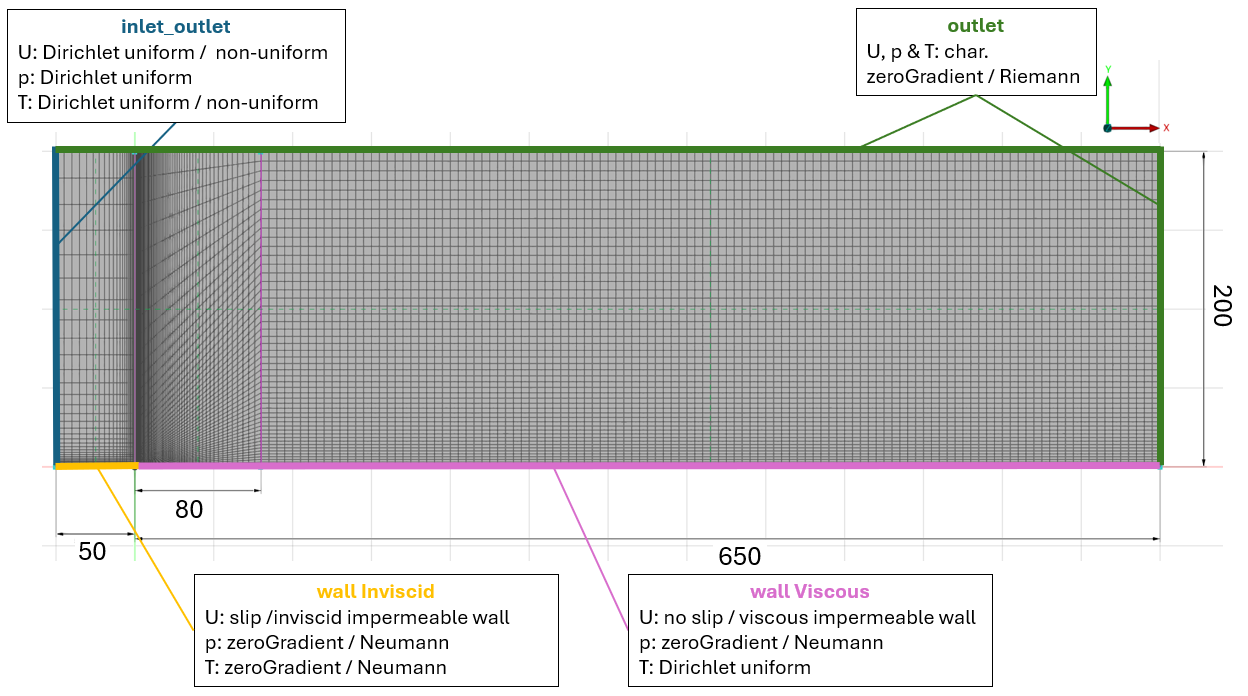
\includegraphics[width=\linewidth,height=.62\textheight,keepaspectratio]{07_Error_Isolation_Results/Figures/WallFunctions/M6Tw025_y+_100_mesh.png}
    \caption{Conventional wall-function mesh for M6Tw025 with nominal first-cell location $y_1^+\approx100$ at the comparison station. Streamwise refinement and a smaller first-cell height resolve the leading-edge region; the wall-normal spacing increases smoothly over the first $80\,\mathrm{mm}$.}
    \label{fig:WF:mesh}
\end{figure}

\begin{figure}[H]
    \centering
    % Figure provenance (WSL; absolute paths):
    %   Figure: /mnt/c/Users/MichaelGnadlinger/OneDrive - Hypersonica/Hypersonica Team - Documents/02 Technical/03 Flight physics/16 Theses/2026/01 Gnadl/Docs_and_Presentations/Thesis_tex/thesis/07_Error_Isolation_Results/Figures/WallFunctions/y+_40_M6Tw025_LiWF_constant.png
    %   Python script: Not applicable: direct ParaView postprocessing screenshot (confirmed by author).
    %   Data / simulation roots (high-level):
    %     /home/mgnadlinger/Xue_et_al/flat_plate/legacy/M6Tw025/LiNeumann_6e-1
    %   Note: No separate export file or plotting script: retained screenshot is at the figure path above.
    %   Note: Association with the listed legacy Li case is inferred from matching mesh geometry and wall-y+
    %     distribution; the original ParaView case path was not recorded.
    % End figure provenance.
    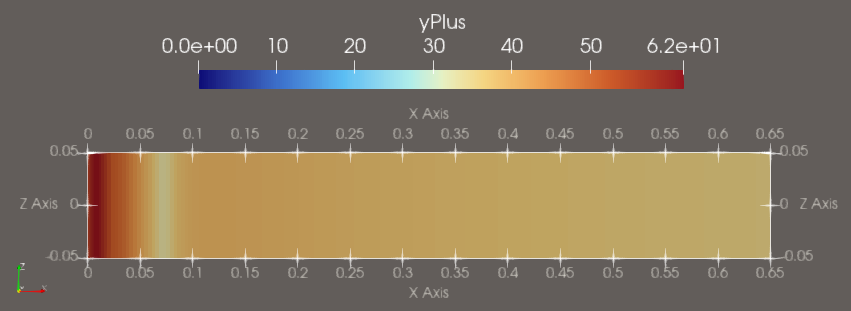
\includegraphics[width=0.7\linewidth,height=.30\textheight,keepaspectratio]{07_Error_Isolation_Results/Figures/WallFunctions/y+_40_M6Tw025_LiWF_constant.png}
    \par\medskip
    % Figure provenance (WSL; absolute paths):
    %   Figure: /mnt/c/Users/MichaelGnadlinger/OneDrive - Hypersonica/Hypersonica Team - Documents/02 Technical/03 Flight physics/16 Theses/2026/01 Gnadl/Docs_and_Presentations/Thesis_tex/thesis/07_Error_Isolation_Results/Figures/WallFunctions/y+_40_M6Tw025_LiWF_smooth.png
    %   Python script: Not applicable: direct ParaView postprocessing screenshot (confirmed by author).
    %   Data / simulation roots (high-level):
    %     /home/mgnadlinger/Xue_et_al/flat_plate/legacy/M6Tw025/LiNeumann_6e-1_smooth
    %   Note: No separate export file or plotting script: retained screenshot is at the figure path above.
    %   Note: Association with the listed legacy Li case is inferred from matching mesh geometry and wall-y+
    %     distribution; the original ParaView case path was not recorded.
    % End figure provenance.
    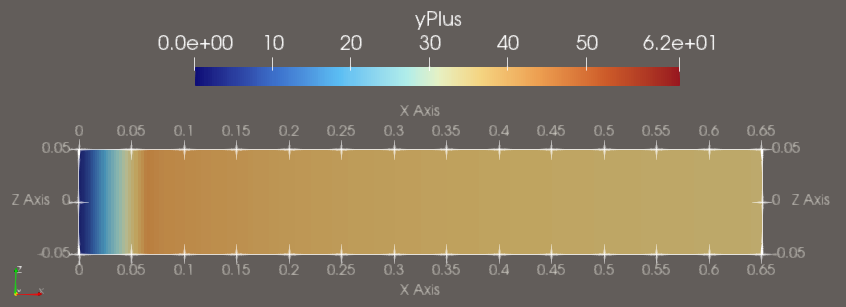
\includegraphics[width=0.7\linewidth,height=.30\textheight,keepaspectratio]{07_Error_Isolation_Results/Figures/WallFunctions/y+_40_M6Tw025_LiWF_smooth.png}
    \caption{Wall-unit first-cell location along the M6Tw025 plate for a nominal $y_1^+\approx40$ Li wall-function mesh. A constant physical first-cell height (top) produces elevated $y_1^+$ near the leading edge. A smooth increase of first-cell height over the first $80\,\mathrm{mm}$ (bottom) reduces this upstream excursion.}
    \label{fig:WF:mesh_constant_smooth}
\end{figure}

Figures~\ref{fig:WF:Li-LowHM3_conventional_mesh}--\ref{fig:WF:Griffin-M6Tw025_conventional_mesh} show the resulting wall heat-flux and shear-stress errors. All curves use the signed relative error to the respective DNS reference at the matched \(Re_{\delta2}\) station (see Section~\ref{subsec:evaluation:matching-station}). The dashed lines show the wall-resolved SA result at the same station as presented and discussed in Section~\ref{sec:comparative:zpg:wall-resolved-baselines}. Around the DNS reference value for th heat-flux and shear stress, the shading marks a $\pm5\%$ error band (as selected in Section~\ref{sec:evaluation:success-criteria}). The horizontal axis shows the actual, calculated first-cell $y_1^+$ at the matched station on these conventional meshes, so each point represents a different CFD simulation with the only change being the first-cell height in the sampling region of the used mesh.
\par\medskip

From Figures~\ref{fig:WF:Li-LowHM3_conventional_mesh}--\ref{fig:WF:Griffin-M6Tw025_conventional_mesh}  it is immediatly visible that the wall-function results are highly sensitive to the first-cell height. But the errors are not monotonic with increasing $y_1^+$, but instead exhibit a pronounced different behaviour in the sublayer region, the buffer and the log-layer region of the cases. The wall-function error bands are also substantially larger than the corresponding a-priori closure variations identified in Section~\ref{subsec:erriso:apriori-results}. Griffin gives signed shear-stress errors of approximately \(-20\%\) to \(+8\%\) and heat-flux errors of \(-16\%\) to \(+12\%\). Over the same cases and sampling-height interval, the Li wall function gives respective shear-stress errors of approximately \(-7\%\) to \(+14\%\) and heat-flux errors of \(-6\%\) to \(+27\%\). But for an engineering context, the high sensitivity of the wall-function results to the first-cell height is arguably more concerning than the absolute error magnitude because it introduces a substantial uncertainty and not a clear bias.
\par\medskip

Looking at the sub-layer region, the wall-function results approach the wall-resolved baseline to within the closure accuracy as expected. Looking at Li's previously found closure behaviour where at \(y^+ = 1\) the wall-function closure error is basically zero (see a-priori result for M6Tw025 in Figure~\ref{fig:wall-closure:a-priori-Li-M6Tw025} and LowH\_M3 in Figure \ref{fig:wall-closure:a-priori-Li-LowHM3}), the wall-function CFD results are also very close to the wall-resolved baseline (see conventional mesh CFD result for M6Tw025 in Figure~\ref{fig:WF:Li-M6Tw025_conventional_mesh} and LowH\_M3 in Figure \ref{fig:WF:Li-LowHM3_conventional_mesh}). The same findings also apply to the Griffin wall-function results where for both cases the a-priori closure assessment in Section~\ref{subsec:erriso:apriori-results} shows a low-$y^+$ closure discrepancy of about $-5\%$ for the wall heat-flux (see a-priori result for M6Tw025 in Figure~\ref{fig:wall-closure:a-priori-Griffin-M6Tw025} and LowH\_M3 in Figure \ref{fig:wall-closure:a-priori-Griffin-LowHM3}), which is also reflected in the deviation of wall-function CFD results from the wall-resolved baseline (see conventional mesh CFD result for M6Tw025 in Figure~\ref{fig:WF:Griffin-M6Tw025_conventional_mesh} and LowH\_M3 in Figure \ref{fig:WF:Griffin-LowHM3_conventional_mesh}).
\par\medskip

Beyond the sublyer, reaching into the buffer layer, the wall-function CFD results do not follow this behaviour where the whole error can be explained through the closure error alone. Rather it is clear that the wall-function CFD results are not only affected by the closure discrepancy, but also by additional error sources. The cause for this behaviour beyond the sublayer is analysed and examined in the next step, where the internal-face fluxues of momentum and energy where compared to the wall-resolved results, and found in the spatial discretization.
\par\medskip

On the even higher $y^+$ conventional meshes, reaching the log-layer and beyond, a sharp reduction in the wall-function CFD error is observed. This reduction does not necessarily indicate a better wall-function performance, but rather indicates a different error sources, that happens to cancel some of the closure discrepancy. In Figure~\ref{fig:WF:Griffin-M6Tw025_conventional_mesh} for example the relative error becomes highly negative, instead of cancelling out to zero. And this behvior in the log-layer and beyond also, as in the buffer layer, do not follow the a-priori seen closure discrepancy. But it is a nice indication why Li et al  found a good agreement of their wall-function CFD results with the DNS reference, because for their validation cases they used a conventional mesh with a first-cell height of \(y^+_1 = 4, 8 \) and then for their cases comfortly in the log-layer \(y^+_1 = 104, 133, 156, 200\) \cite[Figures 17--20 and 23--24]{li2025WF}. Li et al. claim "[...] and it is also essential to avoid them [first grid points] falling into the bufferlayer when using the wall function method." \cite[p. 61]{li2025WF}. So in their analysis they avoided the regions with high sensitivity and large errors, but attributed it to the wrong cause. Griffin et al. use \(y_m=0.3\delta\) for their principal wall-flux comparisons, but also reduce the matching height during WMLES mesh refinement, reaching the buffer region in the lower-Reynolds-number channel case~\cite[Section~4.1]{griffin2023WF}. Their study therefore does not support a blanket exclusion of buffer-layer sampling. As discussed in Section~\ref{subsec:wall-functions:griffin:validation-scope}, those matching-height and LES-resolution studies differ from the present conventional RANS mesh sweeps.

\begin{figure}[H]
    \centering
    % Figure provenance (WSL; absolute paths):
    %   Figure: /home/mgnadlinger/WF_validation/LowH_M3/validation/outputs/plots/li_sa_dns_station_relative_error.png
    %   Python script:
    %     /home/mgnadlinger/WF_validation/LowH_M3/validation/scripts/plot_wall_flux_sweeps.py
    %   Data / simulation roots (high-level):
    %     /home/mgnadlinger/WF_validation/LowH_M3/Li_SA
    %     /home/mgnadlinger/WF_validation/LowH_M3/wall_resolved/SA/LowH_M3
    %     /home/mgnadlinger/WF_validation/LowH_M3/Digitizations
    %   Note: Thesis image removes the 128-pixel title strip from the source export.
    % End figure provenance.
    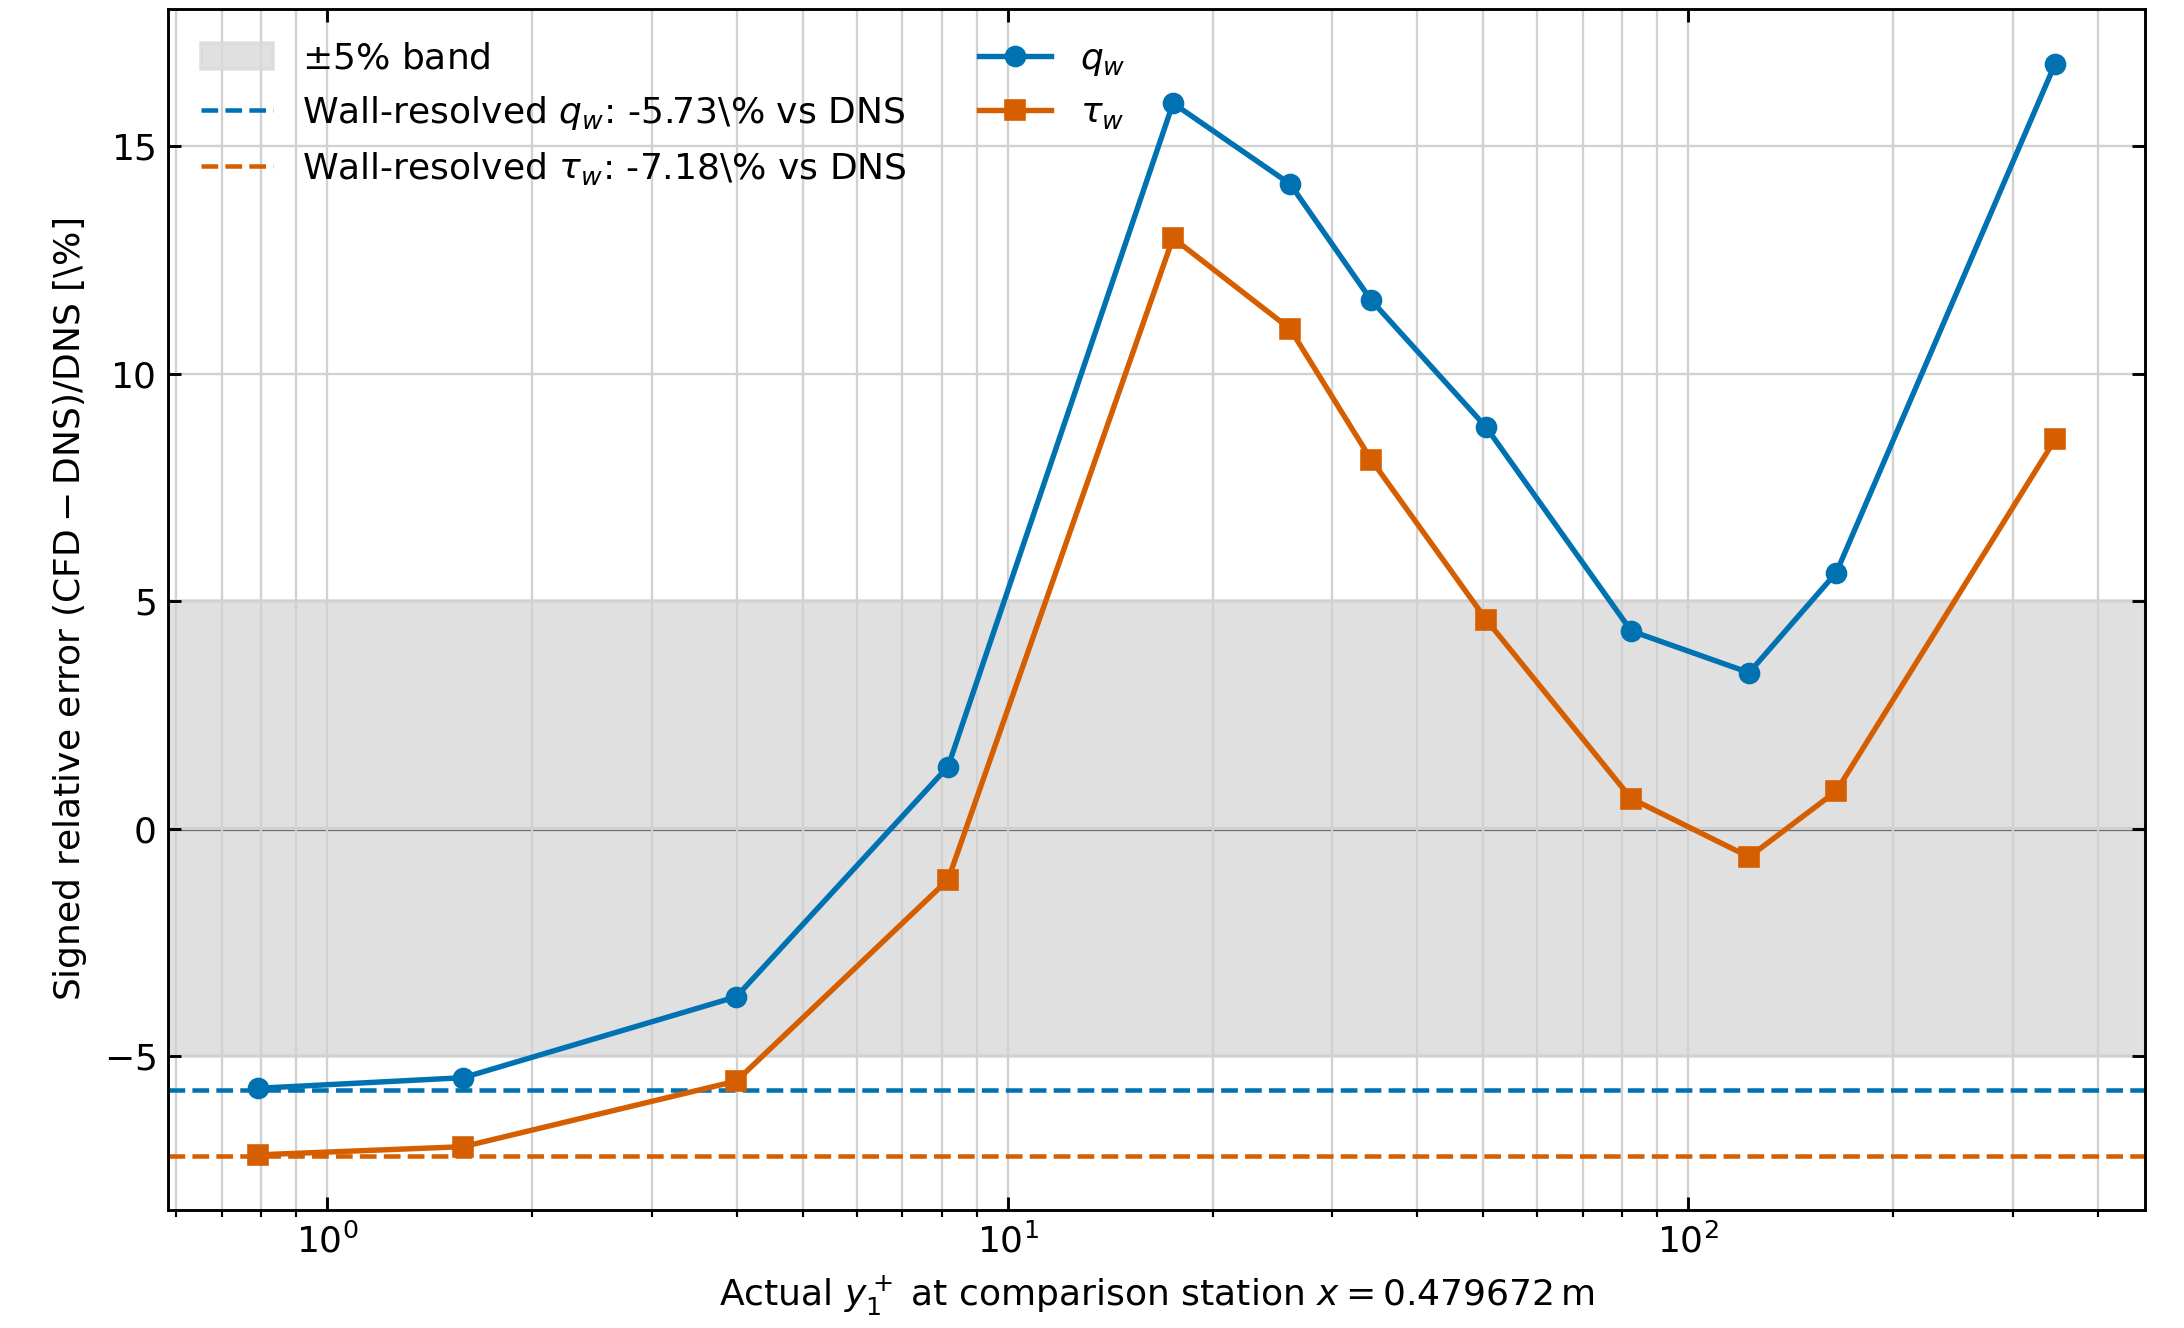
\includegraphics[width=\linewidth,height=.62\textheight,keepaspectratio]{07_Error_Isolation_Results/Figures/WallFunctions/04_ConvMesh_Li_LowHM3.png}
    \caption{Li wall-function CFD with SA on conventional meshes for LowH\_M3: signed errors in wall heat-flux $q_w$ and shear stress $\tau_w$ relative to DNS, evaluated at $x=0.479672\,\mathrm{m}$ against the actual first-cell $y_1^+$. Dashed lines denote the wall-resolved SA errors; shading marks $\pm5\%$ relative to DNS.}
    \label{fig:WF:Li-LowHM3_conventional_mesh}
\end{figure}

\begin{figure}[H]
    \centering
    % Figure provenance (WSL; absolute paths):
    %   Figure: /home/mgnadlinger/WF_validation/LowH_M3/validation/outputs/plots/griffin_sa_dns_station_relative_error.png
    %   Python script:
    %     /home/mgnadlinger/WF_validation/LowH_M3/validation/scripts/plot_wall_flux_sweeps.py
    %   Data / simulation roots (high-level):
    %     /home/mgnadlinger/WF_validation/LowH_M3/Griffin_SA
    %     /home/mgnadlinger/WF_validation/LowH_M3/wall_resolved/SA/LowH_M3
    %     /home/mgnadlinger/WF_validation/LowH_M3/Digitizations
    % End figure provenance.
    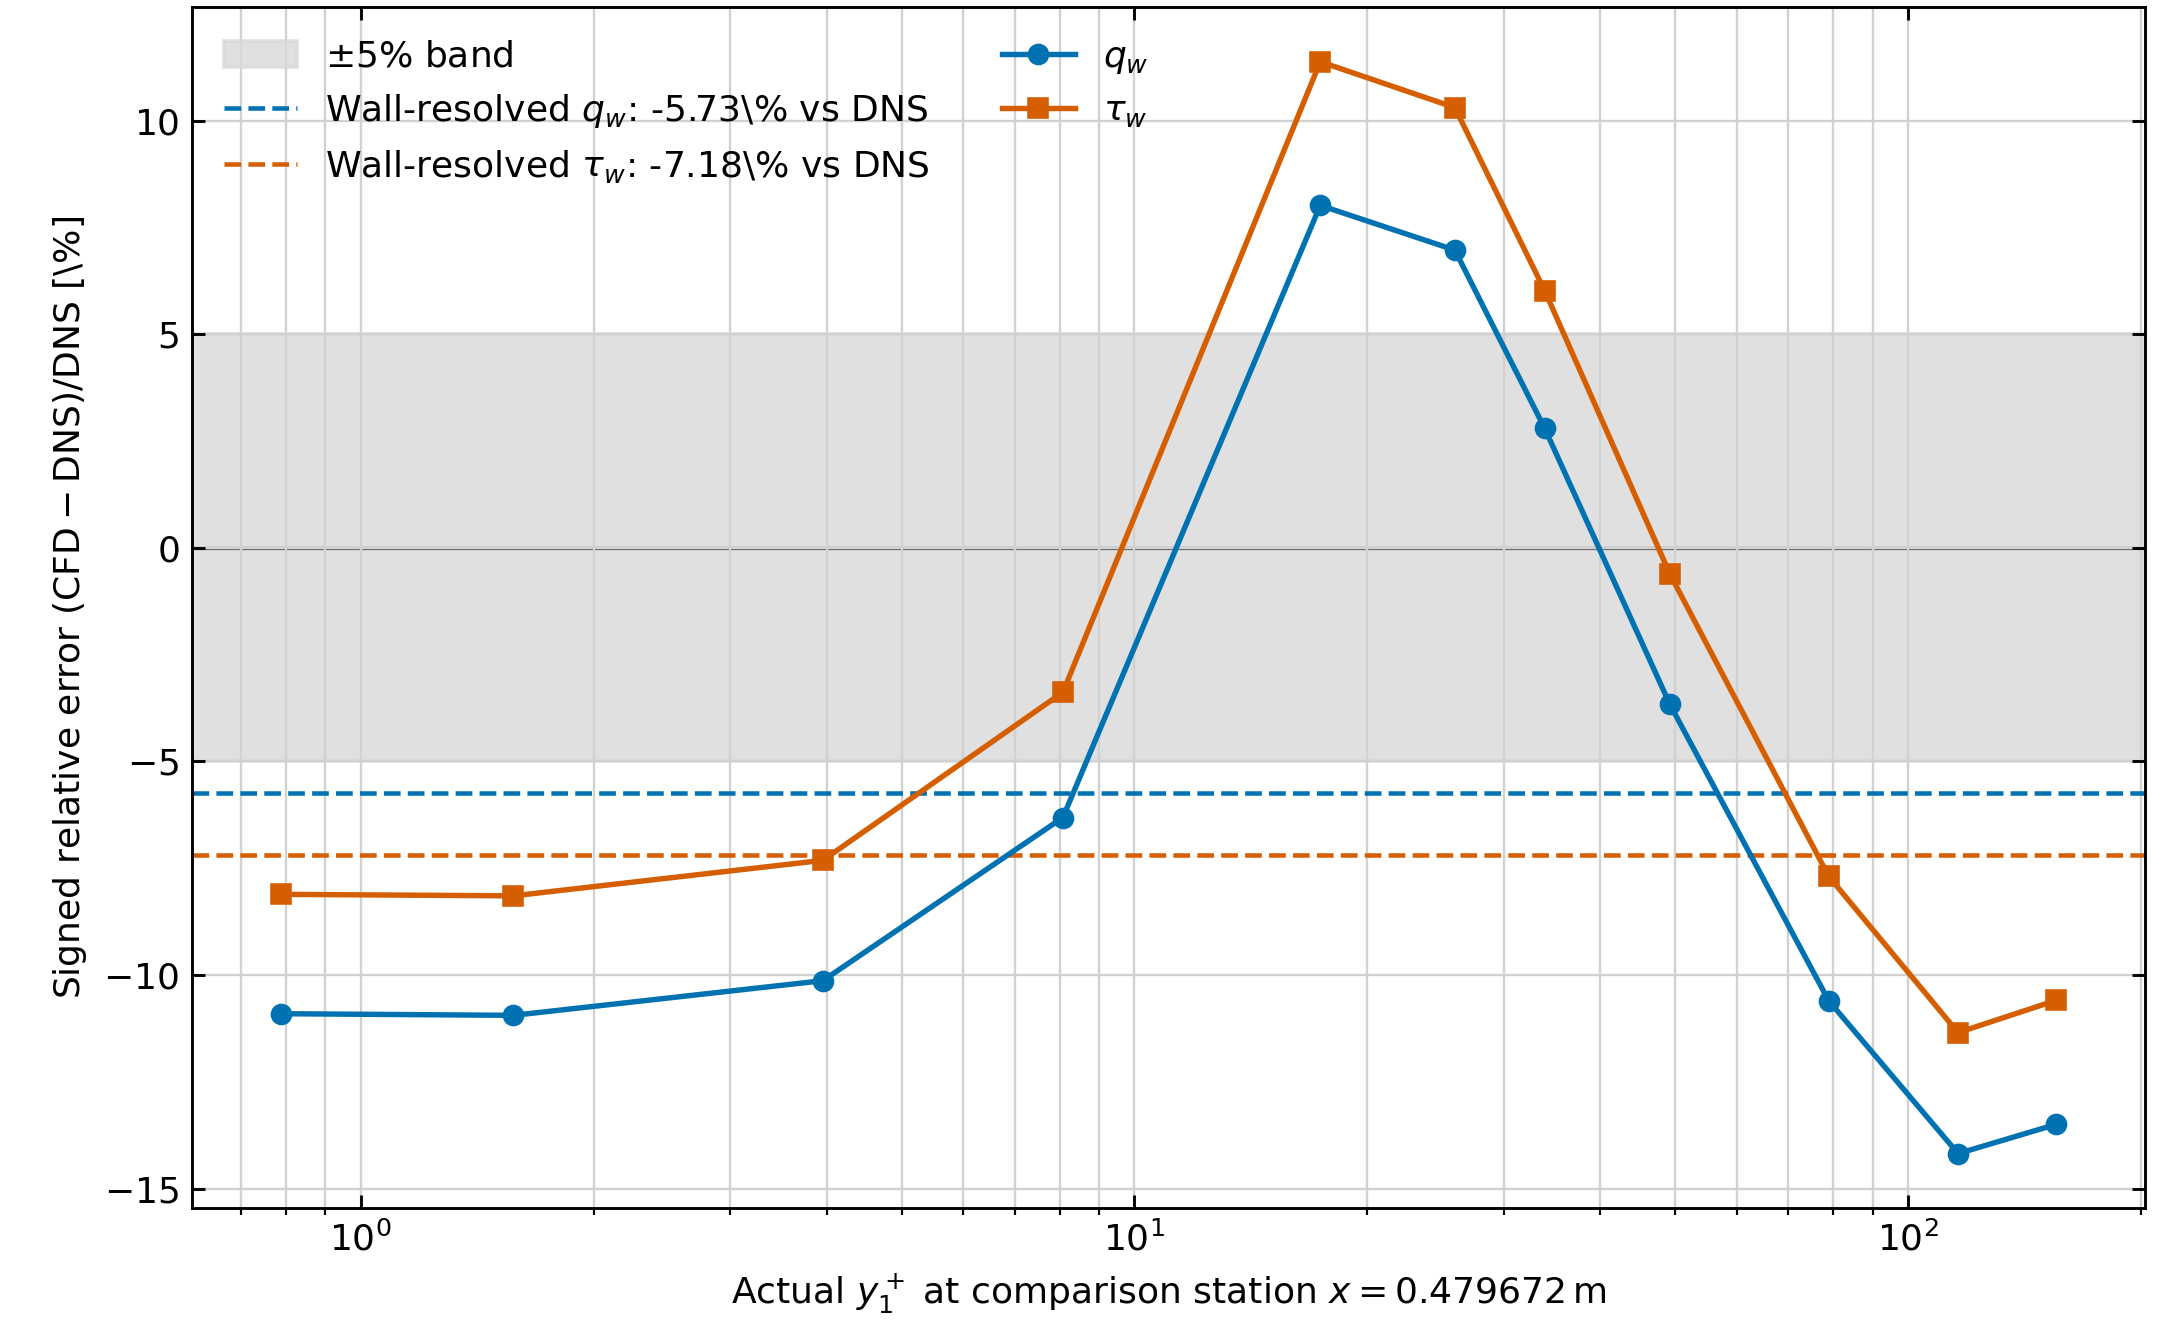
\includegraphics[width=\linewidth,height=.62\textheight,keepaspectratio]{07_Error_Isolation_Results/Figures/WallFunctions/04_ConvMesh_Griffin_LowHM3.png}
    \caption{Griffin wall-function CFD with SA on conventional meshes for LowH\_M3. Wall heat-flux and shear-stress errors use the same DNS normalization and comparison station as Figure~\ref{fig:WF:Li-LowHM3_conventional_mesh}. Dashed lines denote the wall-resolved baseline; shading marks $\pm5\%$ relative to DNS.}
    \label{fig:WF:Griffin-LowHM3_conventional_mesh}
\end{figure}

\begin{figure}[H]
    \centering
    % Figure provenance (WSL; absolute paths):
    %   Figure: /home/mgnadlinger/Xue_et_al/flat_plate/M6Tw025/validation/outputs_Li_SA/group1_wall_flux_relative_error_vs_yplus.png
    %   Python script:
    %     /home/mgnadlinger/Xue_et_al/flat_plate/M6Tw025/validation/plot_wall_fluxes_and_figure6.py
    %   Data / simulation roots (high-level):
    %     /home/mgnadlinger/Xue_et_al/flat_plate/M6Tw025/Li_SA
    %     /home/mgnadlinger/Xue_et_al/flat_plate/M6Tw025/Li_SA/SA_Prt0p9_baseline
    %     /home/mgnadlinger/Xue_et_al/flat_plate/M6Tw025/Digitizations
    %     /home/mgnadlinger/Zhang_DNS_ZPGFP/References/Data
    %   Note: Thesis image removes the 128-pixel title strip from the source export.
    % End figure provenance.
    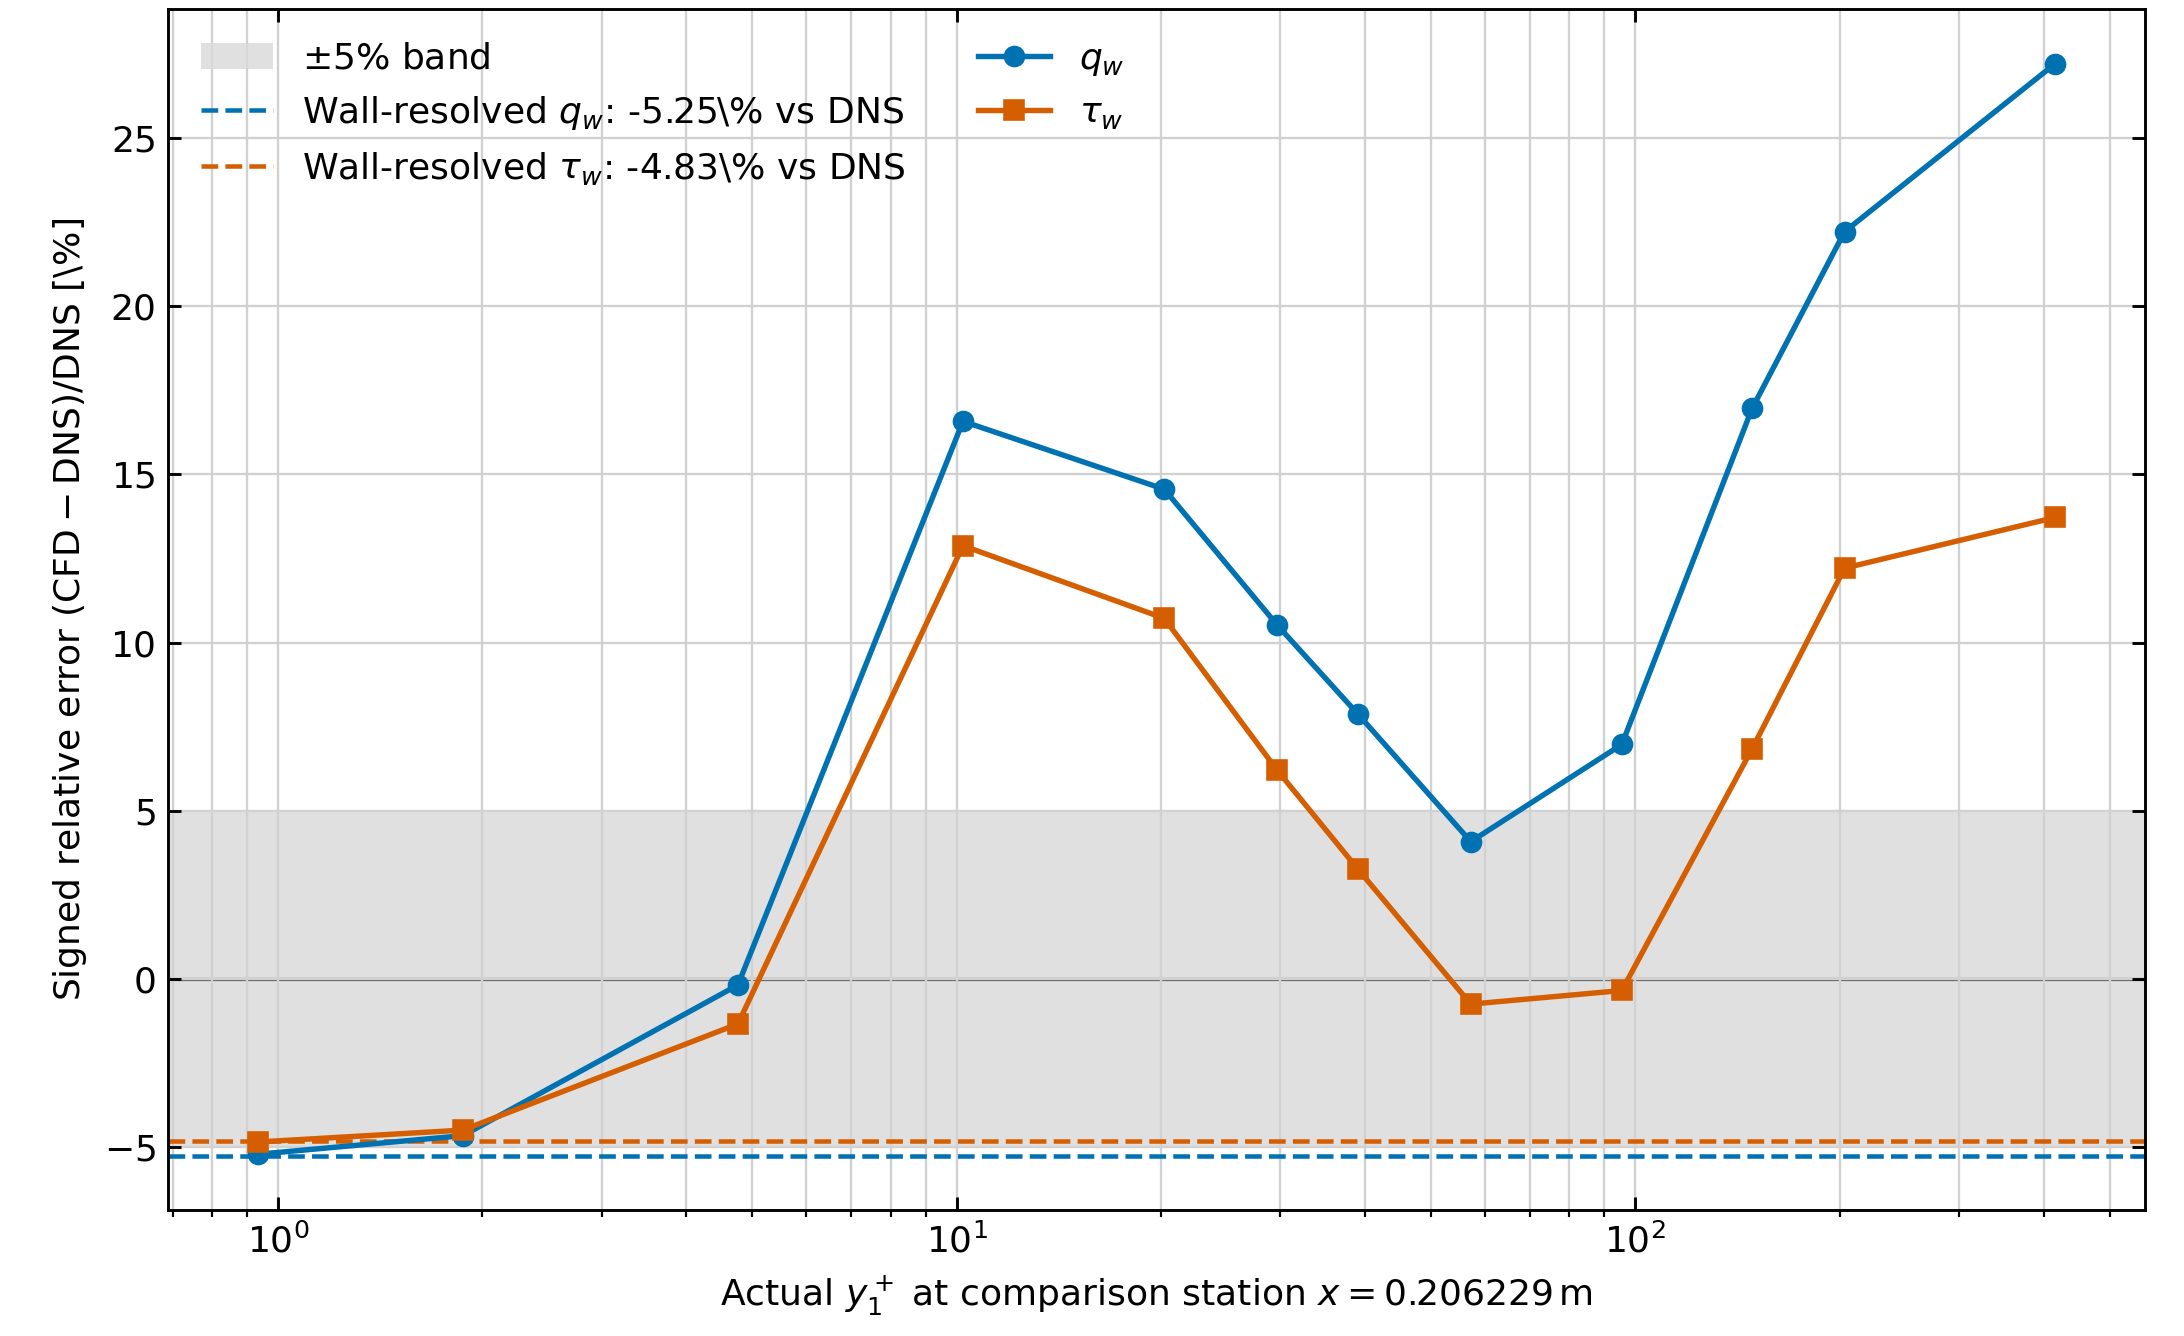
\includegraphics[width=\linewidth,height=.62\textheight,keepaspectratio]{07_Error_Isolation_Results/Figures/WallFunctions/04_ConvMesh_Li_M6Tw025.png}
    \caption{Li wall-function CFD with SA on conventional meshes for M6Tw025: signed wall heat-flux and shear-stress errors relative to DNS at $x=0.206229\,\mathrm{m}$ against the actual first-cell $y_1^+$. Dashed lines denote the wall-resolved SA errors; shading marks $\pm5\%$ relative to DNS.}
    \label{fig:WF:Li-M6Tw025_conventional_mesh}
\end{figure}

\begin{figure}[H]
    \centering
    % Figure provenance (WSL; absolute paths):
    %   Figure: /home/mgnadlinger/Xue_et_al/flat_plate/M6Tw025/validation/outputs_Griffin_SA/group1_wall_flux_relative_error_vs_yplus.png
    %   Python script:
    %     /home/mgnadlinger/Xue_et_al/flat_plate/M6Tw025/validation/plot_wall_fluxes_and_figure6.py
    %   Data / simulation roots (high-level):
    %     /home/mgnadlinger/Xue_et_al/flat_plate/M6Tw025/Griffin_SA
    %     /home/mgnadlinger/Xue_et_al/flat_plate/M6Tw025/Griffin_SA/SA_Prt0p9_baseline
    %     /home/mgnadlinger/Xue_et_al/flat_plate/M6Tw025/Digitizations
    %     /home/mgnadlinger/Zhang_DNS_ZPGFP/References/Data
    % End figure provenance.
    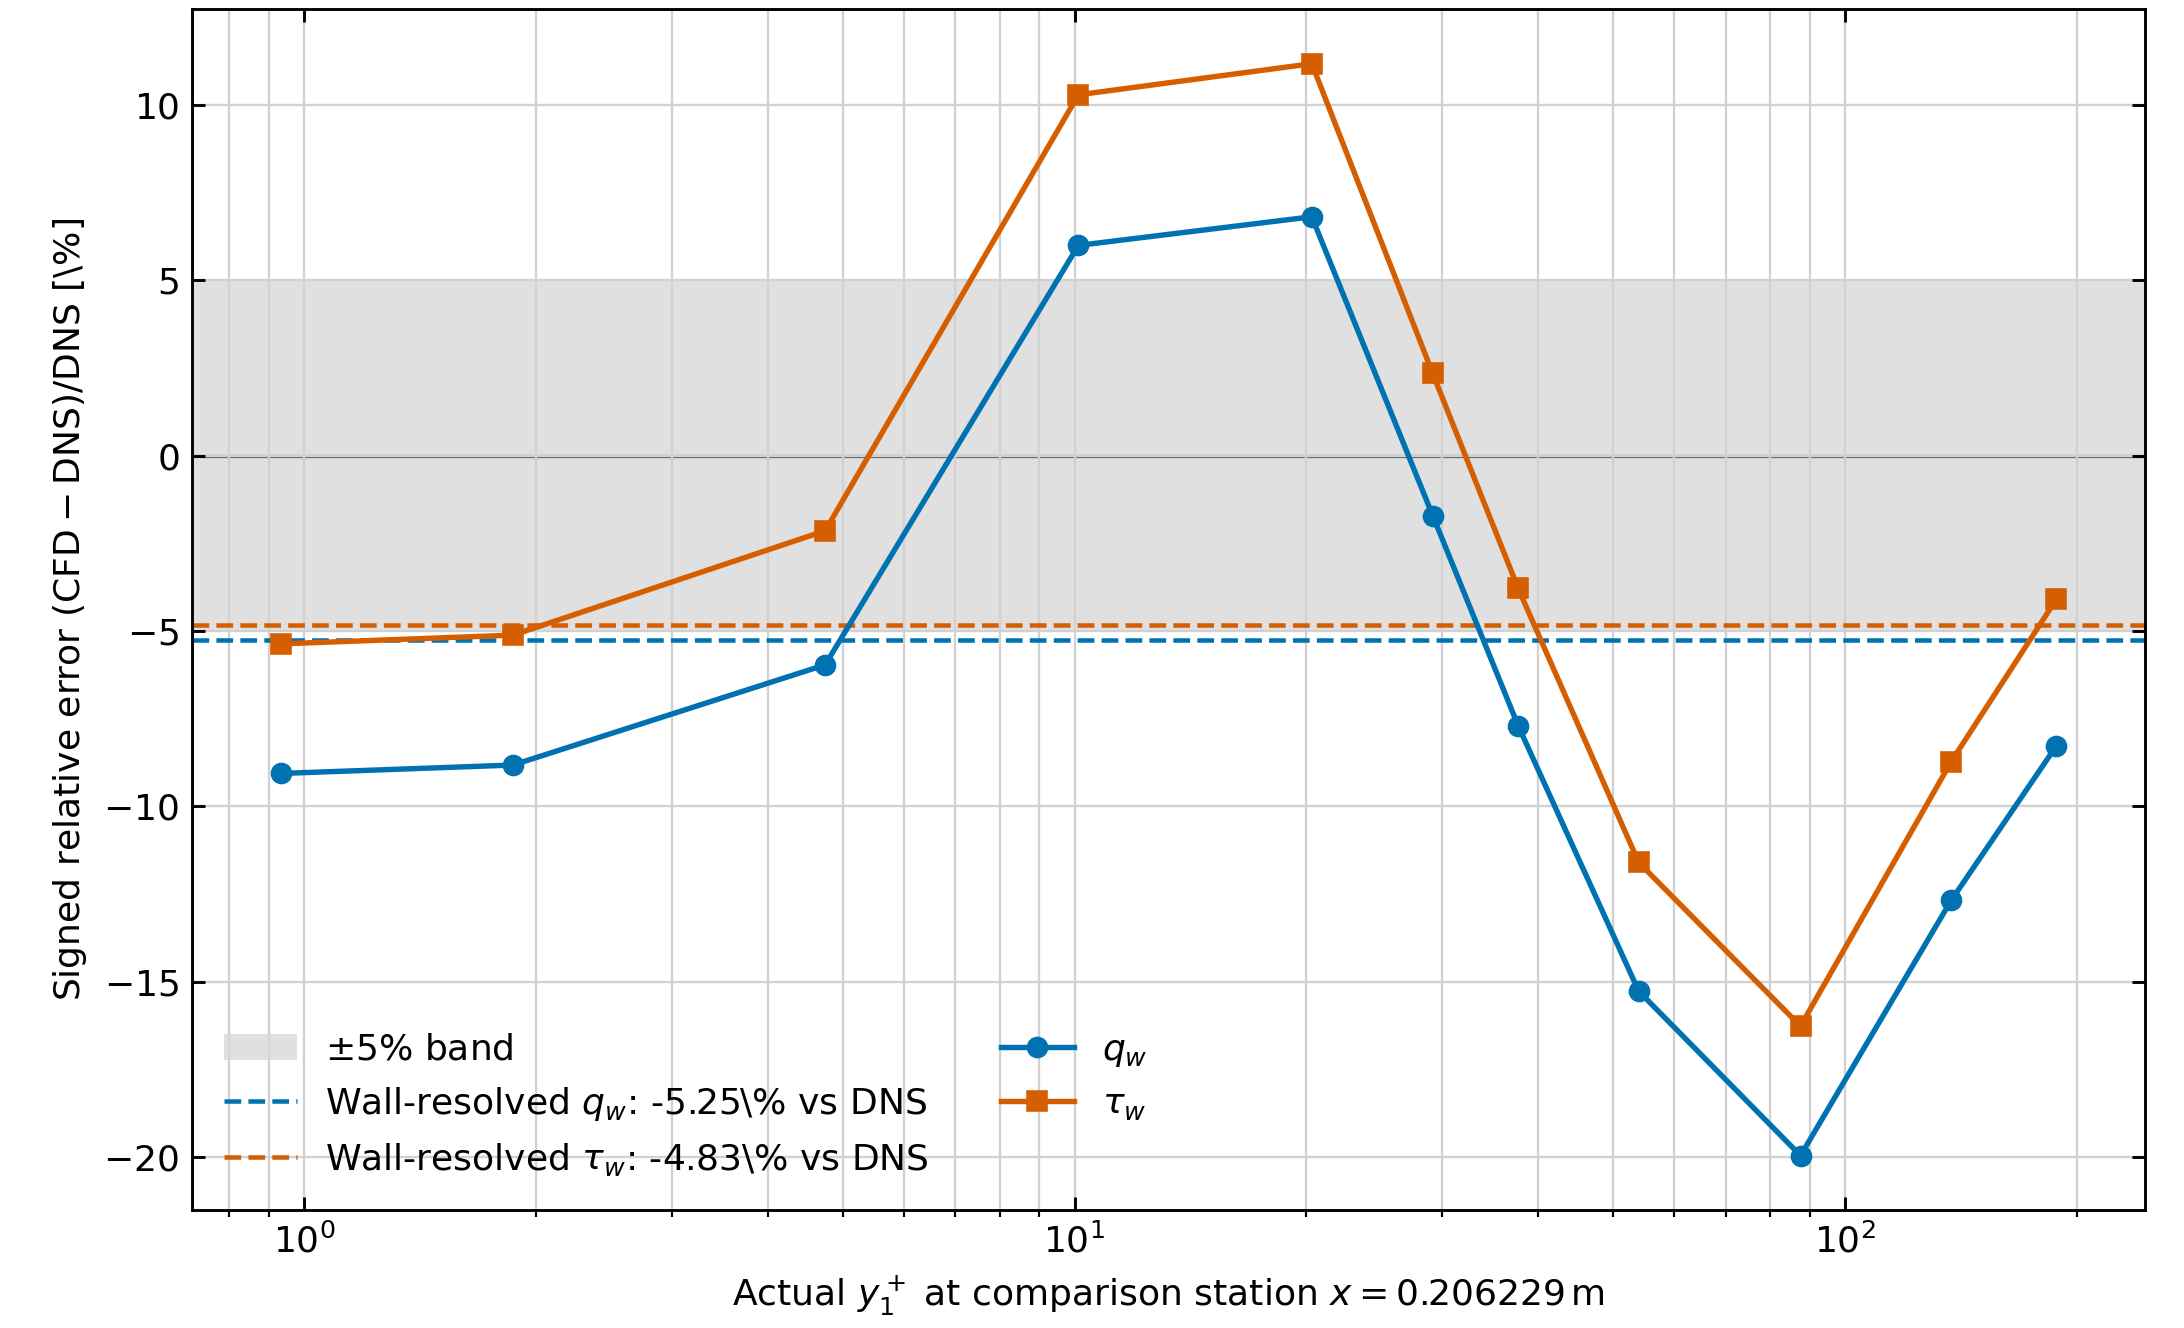
\includegraphics[width=\linewidth,height=.62\textheight,keepaspectratio]{07_Error_Isolation_Results/Figures/WallFunctions/04_ConvMesh_Griffin_M6Tw025.png}
    \caption{Griffin wall-function CFD with SA on conventional meshes for M6Tw025, using the DNS normalization and station of Figure~\ref{fig:WF:Li-M6Tw025_conventional_mesh}. Dashed lines denote the wall-resolved baseline; shading marks $\pm5\%$ relative to DNS.}
    \label{fig:WF:Griffin-M6Tw025_conventional_mesh}
\end{figure}

\subsection{Internal-face errors and a wall-normal spacing criterion}
\label{subsec:comparative:zpg:mesh-criterion}

For the FVM CFD, the numerical framework, is described in Section~\ref{sec:numerical-framework:discretization} and
distinguishes convective reconstruction from viscous flux evaluation. The direct wall-flux delivery of the wall-functions, as described in Section~\ref{subsec:wall-functions:direct-flux-delivery}, replaces the gradient-based evaluation at the wall, but gradients and transport coefficients at internal faces must still be approximated from the cell-centre values. For a predominantly streamwise boundary layer flow, neglecting $\partial V/\partial x$ relative to $\partial U/\partial y$ gives
\begin{equation}
    \tau_{xy}\simeq\mu_{\mathrm{eff}}\frac{\partial U}{\partial y},
    \qquad
    q_y=-\kappa_{\mathrm{eff}}\frac{\partial T}{\partial y}.
    \label{eq:erriso:diffusive-face-fluxes}
\end{equation}
Here $\tau_{xy}$ is the effective shear stress and $q_y$ is the effective heat-flux in the positive wall-normal direction. At internal faces parallel to the wall, these fluxes contribute to the discrete momentum and energy balances. As Equation~\ref{eq:erriso:diffusive-face-fluxes} shows, their evaluation relies both on wall-normal gradient approximations as well as interpolation of the effective viscosity $\mu_{\mathrm{eff}}$ and thermal conductivity $\kappa_{\mathrm{eff}}$ at the face location. Errors in either can therefore alter the flow field solution, which in turn feeds into the wall-function.
\par\medskip

Figure~\ref{fig:WF:exemplaray_y+10_mesh} visualizes the geometry of these operations on an exemplary conventional coarse wall-function mesh with a first-cell height of $y_1^+=10$ on the left and $y_1^+=30$ on the right. For equal adjacent cell thicknesses, the first centre at $y_1^+=10$ and the next at $y_2^+=30$ surround the internal face at $y_f^+=20$. The full centre separation, which the gradient approximation and coefficient interpolation needs to gap, is thus $h^+=20$. Increasing the first-cell height to $y_1^+=30$ also increases the stencil separation to $y_f^+=h^+=60$. Thus conventional coarsening changes both the wall-function sampling height and the distance over which internal-face transport is evaluated. The former already isolately evaluated in Section~\ref{sec:comparative:zpg:cross-comparison} and the latter is evaluated in this section.

\begin{figure}[H]
    \centering
    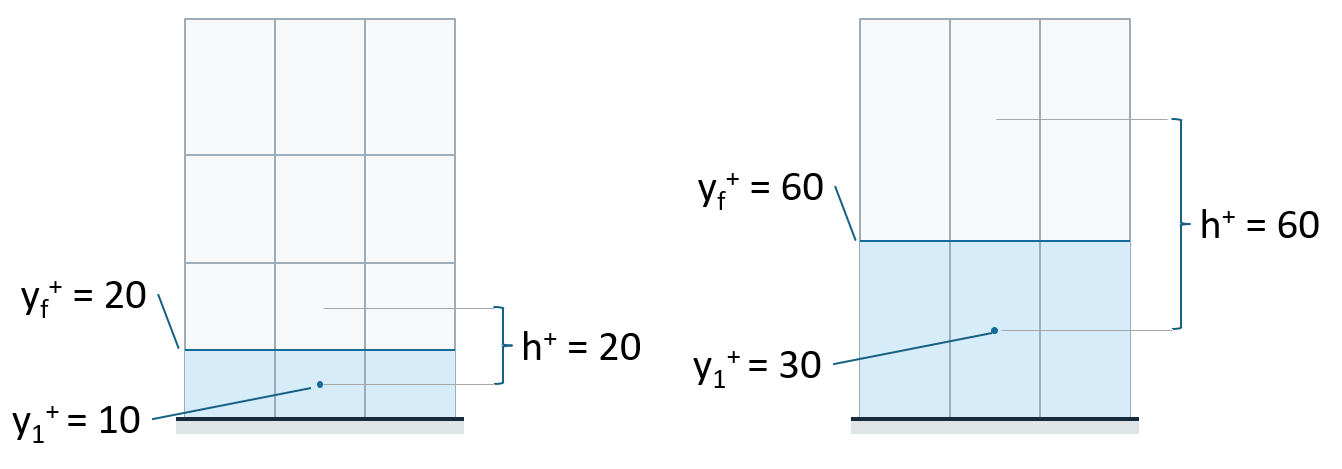
\includegraphics[width=\linewidth,height=.62\textheight,keepaspectratio]{07_Error_Isolation_Results/Figures/Recon/illustration_conv_coarse_mesh.png}
    \caption{Illustrative conventional near-wall meshes. For equal cell thicknesses adjacent to the first internal face, $y_1^+=10$ gives $y_f^+=h^+=20$ (left), while $y_1^+=30$ gives $y_f^+=h^+=60$ (right). Here $h^+$ is the full centre separation. The lower cell extends from the wall to the face, establishing an upper geometric link between the centre spacing $h^+$ and cell height of $h^+=y_f^+$.}
    \label{fig:WF:exemplaray_y+10_mesh}
\end{figure}

Figure~\ref{fig:WF:exemplaray_y+10_reconstruction_error} uses the M6Tw025 DNS temperature profile to illustrate a potential limitation of second-order accurate internal-face gradient reconstruction in a hypersonic cold-wall boundary layer. For the symmetric two-centre stencil considered here, the second-order accurate face-gradient approximation is the slope of a linear secant through the neighbouring cell-centre values. In this example, the secant connects the temperatures at $y^+=10$ and $30$, while the required gradient is the tangent slope at $y_f^+=20$. The pronounced cold-wall temperature peak causes substantial variation in curvature across this coarse stencil, and the two slopes differ visibly. Thus even a symmetric, second-order accurate approximation can poorly represent the local thermal gradient. This example illustrates the mechanism, while the spacing analysis below quantifies it over the profile. Here second-order accuracy refers to the leading error scaling with the square of the centre separation, not to a quadratic interpolating curve.

\begin{figure}[H]
    \centering
    % Figure provenance (WSL; absolute paths):
    %   Figure: /mnt/c/Users/MichaelGnadlinger/.codex/visualizations/2026/09/28/01a0e8e6-c3e6-7e32-a912-308b04eb3ffd/M6Tw025_temperature_profile_clean_600.png
    %   Python script:
    %     /mnt/c/Users/MichaelGnadlinger/.codex/visualizations/2026/09/28/01a0e8e6-c3e6-7e32-a912-308b04eb3ffd/plot_temperature_profile_clean_600.py
    %   Data / simulation roots (high-level):
    %     /home/mgnadlinger/Xue_et_al/flat_plate/M6Tw025/opt_mesh/reference
    %     /home/mgnadlinger/Xue_et_al/flat_plate/M6Tw025/Digitizations
    %   Note: Thesis image is resized and cropped to remove the title.
    % End figure provenance.
    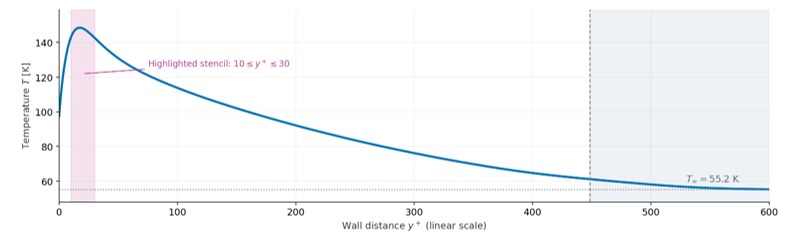
\includegraphics[width=\linewidth,height=.30\textheight,keepaspectratio]{07_Error_Isolation_Results/Figures/Recon/example_M6Tw025_Temperature_profile.png}
    \par\medskip
    % Figure provenance (WSL; absolute paths):
    %   Figure: /mnt/c/Users/MichaelGnadlinger/.codex/visualizations/2026/09/10/01a08aab-7a88-7450-b58c-b4f35bd01e8a/M6Tw025_temperature_full_and_y20.png
    %   Python script:
    %     /mnt/c/Users/MichaelGnadlinger/.codex/visualizations/2026/09/10/01a08aab-7a88-7450-b58c-b4f35bd01e8a/plot_temperature_y20.py
    %   Data / simulation roots (high-level):
    %     /home/mgnadlinger/Xue_et_al/flat_plate/M6Tw025/opt_mesh/reference
    %     /home/mgnadlinger/Xue_et_al/flat_plate/M6Tw025/Digitizations
    %   Note: Thesis image is a resized crop of panel (b), Temperature near the maximum.
    % End figure provenance.
    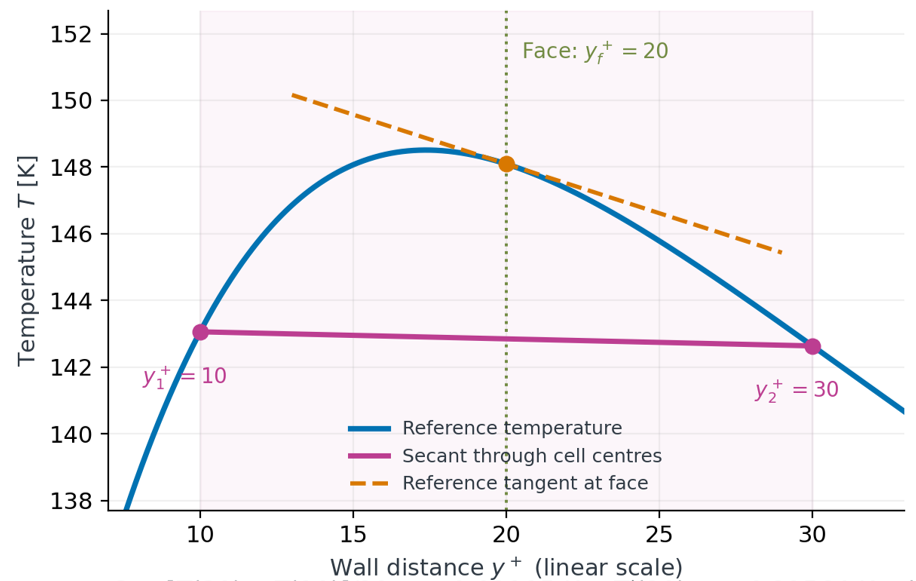
\includegraphics[width=\linewidth,height=.30\textheight,keepaspectratio]{07_Error_Isolation_Results/Figures/Recon/example_M6Tw025_Temperature_zoomed.png}
    \caption{M6Tw025 DNS temperature profile (top) and detail near its maximum (bottom). For the illustrative stencil in Figure~\ref{fig:WF:exemplaray_y+10_mesh}, the purple secant between $y^+=10$ and $30$ differs from the local tangent at the internal face $y_f^+=20$ (orange dashed line). The slopes illustrate the gradient contribution to thermal-diffusion error; the corresponding face flux also depends on the interpolated effective conductivity.}
    \label{fig:WF:exemplaray_y+10_reconstruction_error}
\end{figure}

The two-centre face-gradient approximation of a second-order accurate gradient reconstruction scheme is the slope of the linear secant through the neighbouring profile values:
\begin{equation}
    D_f\phi=\frac{\phi(y_R)-\phi(y_L)}{y_R-y_L}
    =\frac{\phi(y_f+b)-\phi(y_f-a)}{a+b},
    \qquad \phi\in\{T,U\},
\end{equation}
where $a=y_f-y_L$, $b=y_R-y_f$ and $h=a+b$. Unequal spacing introduces a truncation-error contribution $(b-a)\phi''(y_f)/2$. For the symmetric stencil, $a=b=h/2$, however this contribution vanishes and the secant slope approximates the face gradient with second-order accuracy. Taylor expansion expresses the secant slope as the exact tangent slope plus its error:
\begin{equation}
    \frac{\phi(y_f+h/2)-\phi(y_f-h/2)}{h}
    =\phi'(y_f)+\frac{h^2}{24}\phi'''(y_f)+O(h^4),
    \qquad \phi\in\{T,U\}.
    \label{eq:erriso:symmetric-gradient}
\end{equation}
For this symmetric stencil, the leading gradient error therefore depends on the change in curvature, $\phi'''$, rather than curvature alone. Dividing its magnitude by $|\phi'(y_f)|$ and prescribing a relative accuracy of the face gradient $\epsilon$ gives the spacing estimation $h_{\mathrm{grad}}$ for the second order accurate gradient reconstruction on a symmetric stencil as
\begin{equation}
    h_{\mathrm{grad}}\simeq
    \sqrt{24\epsilon\left|\frac{\phi'}{\phi'''}\right|}.
    \label{eq:erriso:gradient-spacing}
\end{equation}
Similarly, for symmetric linear interpolation of a coefficient $\Gamma\in\{\mu_{\mathrm{eff}},\kappa_{\mathrm{eff}}\}$, the face value is approximated by the mean of the two cell-centre values. Its leading error is $h^2\Gamma''(y_f)/8$, giving
\begin{equation}
    h_{\mathrm{interp}}\simeq
    \sqrt{8\epsilon\left|\frac{\Gamma}{\Gamma''}\right|}.
    \label{eq:erriso:coefficient-spacing}
\end{equation}
Equations~\eqref{eq:erriso:symmetric-gradient}--\eqref{eq:erriso:coefficient-spacing} identify the profile derivatives controlling the two operations. The envelopes below evaluate the corresponding finite-stencil errors directly on cubic-interpolation reconstructions of the digital reference profiles. The resulting spacing limits are the maximum centre separation that satisfies a prescribed relative error $\epsilon$ for each operation. 
\par\medskip

Figure~\ref{fig:WF:M6Tw025-profiles} shows exemplary the four profiles of the M6Tw025 case passed through this spacing analysis. DNS supplies M6Tw025 temperature and velocity, the matched wall-resolved SA solution supplies effective viscosity and conductivity. The effective transport properties need to be taken from the wall-resolved SA reference because not published with the DNS profiles. For the subsequent LowH\_M3 mesh design, all profiles come from the wall-resolved SA reference, because of the lack of published high-quality digital DNS data. In the Figure~\ref{fig:WF:M6Tw025-profiles} profiles it is immediatly apparant that the thermal profile present significantly more change in curvature than the velocity profile because of the sharp temperature peak near the wall. As identified in Equation~\eqref{eq:erriso:coefficient-spacing}, the transport coefficients rely on the curvature of the repsetive profiles, rather than the change in curvature, which for the M6Tw025 case has three pronounced regions of high curvature, directly at the wall because of the zero gradient Neumann boundary conditions there, at \(y \approx 0.0025 \mathrm{m}\) and \(y \approx 0.005 \mathrm{m}\) (see Figure~\ref{fig:WF:M6Tw025-profiles} bottom plots). 

\begin{figure}[H]
    \centering
    % Figure provenance (WSL; absolute paths):
    %   Figure: /home/mgnadlinger/Xue_et_al/flat_plate/M6Tw025/opt_mesh/spacing_limits/M6Tw025_DNS_and_wall_resolved_profiles_physical_y_linear.png
    %   Python script:
    %     /home/mgnadlinger/Xue_et_al/flat_plate/M6Tw025/opt_mesh/scripts/plot_requested_profiles.py
    %   Data / simulation roots (high-level):
    %     /home/mgnadlinger/Xue_et_al/flat_plate/M6Tw025/opt_mesh/reference
    %     /home/mgnadlinger/Xue_et_al/flat_plate/M6Tw025/Digitizations
    %     /home/mgnadlinger/Xue_et_al/flat_plate/M6Tw025/Li_SA/SA_Prt0p9_baseline
    %   Note: DNS temperature/velocity and SA effective transport use the frozen reference package; the SA
    %     station is x = 0.206229 m at time 15000.
    % End figure provenance.
    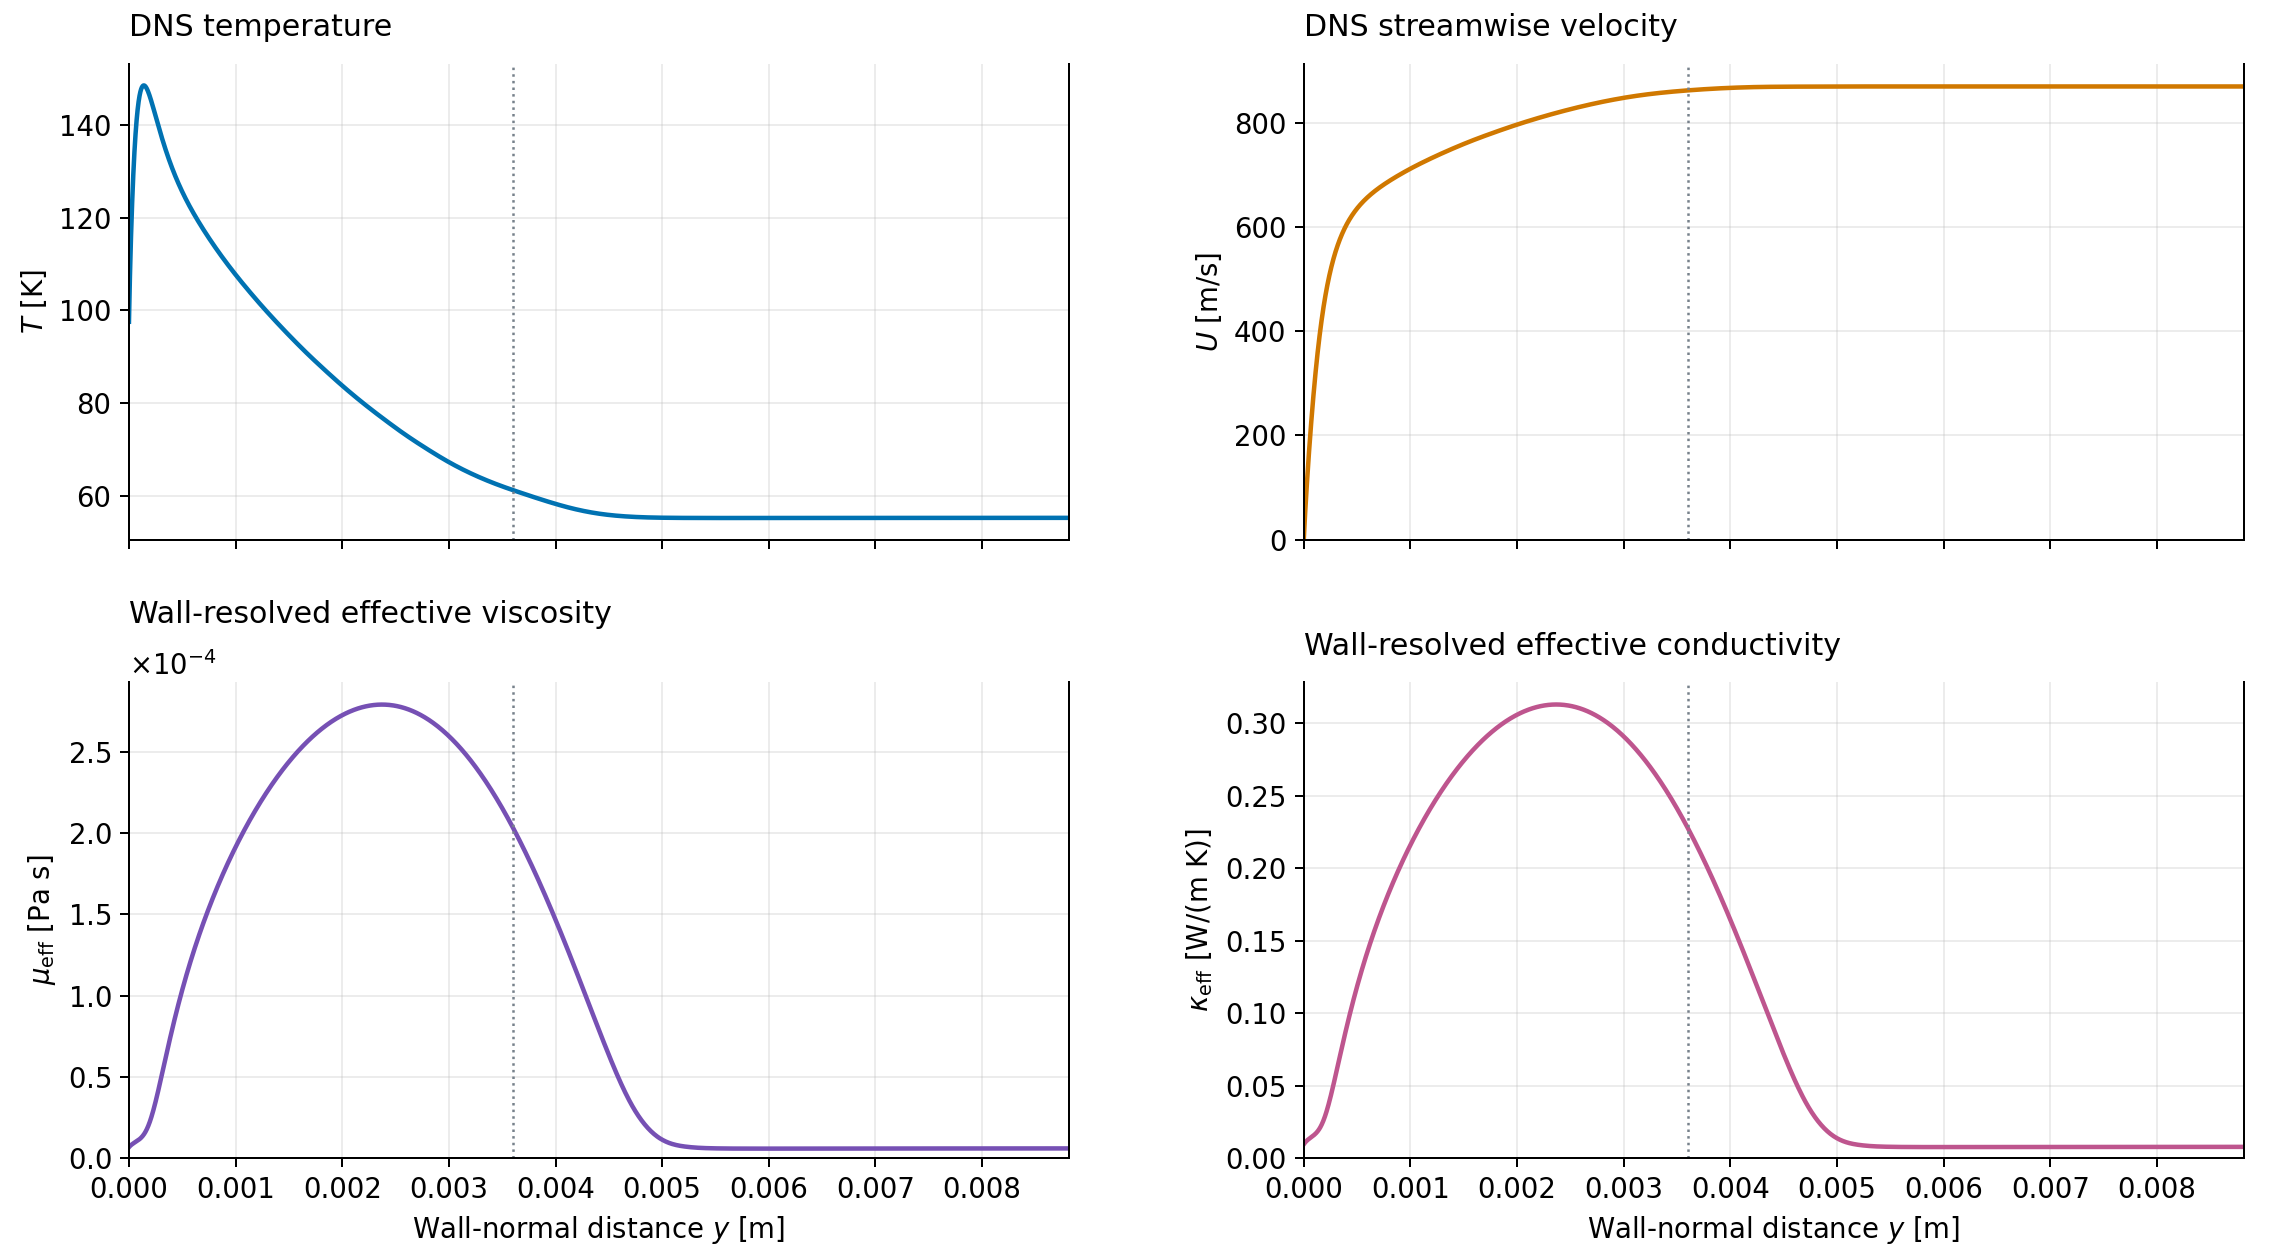
\includegraphics[width=\linewidth,height=.62\textheight,keepaspectratio]{07_Error_Isolation_Results/Figures/Recon/M6Tw025_DNS_BL_profiles_lin-y.png}
    \caption{Profiles underlying the M6Tw025 spacing assessment, plotted against physical wall-normal distance. DNS temperature and velocity are shown above; effective viscosity and thermal conductivity from the matched wall-resolved SA solution are shown below. The temperature maximum and the variation of effective transport motivate separate gradient and coefficient-interpolation criteria.}
    \label{fig:WF:M6Tw025-profiles}
\end{figure}

Using the found Equations \eqref{eq:erriso:gradient-spacing} and \eqref{eq:erriso:coefficient-spacing} that link the cell-centre spacing to the respective gradient reconstruction and interpolation errors, the M6Tw025 profiles of Figure~\ref{fig:WF:M6Tw025-profiles} are analysed. This results in the four individual spacing limits as shown in Figure~\ref{fig:WF:M6Tw025-3pct-envelope-all-quantities}. The resulting envelopes show, the allowable cell spacing $h$, for a given cell face position $y^+_f$ so that the relative errors for the gradient reconstruction or interpolation stay below a given tolerance of e.g. $\epsilon_{max}=3\%$.
\par\medskip

The cell spacing must also adhere to the upper geometric limit of $h^+\leq y_f^+$. At this limit two equal hight cells around a given face have centres at $y_f^+/2$ and $3y_f^+/2$, thus resulting in the lower cell extending all the way from the face to the wall. Thus the full centre separation equals the face-to-wall distance. This is the conventional coarse wall-function mesh geometry illustrated above in Figure~\ref{fig:WF:exemplaray_y+10_mesh}. A limit below this line requires a smaller centre separation at the same face position. a limit reaching it permits that conventional stencil under the selected local criterion. The cap is an adopted mesh constraint, not an error estimate.
\par\medskip

Figure~\ref{fig:WF:M6Tw025-3pct-envelope-all-quantities} shows the individual limits for $\epsilon=0.03$. The temperature-gradient limit has a sharp minimum near the temperature maximum as expected and hypthesized above. The coefficient interpolation and velocity-gradient reconstruction somewhat restrict other parts of the inner layer. At the exact Temperature peak, $T'=0$ thus the relative gradient error of Equations \eqref{eq:erriso:gradient-spacing} appraoches a asymptote - for the M6Tw025 case this is at around $y^+_f\approx 18$, in-line with the plotted temperature profile in Figure~\ref{fig:WF:exemplaray_y+10_reconstruction_error}. The sharp minimum reflects this conditioning as good as the cubic-interpolation of the given profile allows.

\begin{figure}[H]
    \centering
    % Figure provenance (WSL; absolute paths):
    %   Figure: /home/mgnadlinger/Xue_et_al/flat_plate/M6Tw025/opt_mesh/spacing_limits/M6Tw025_finite_spacing_3pct_relative_no_diagnostic_note.png
    %   Python scripts:
    %     /home/mgnadlinger/Xue_et_al/flat_plate/M6Tw025/opt_mesh/scripts/plot_requested_profiles.py
    %     /home/mgnadlinger/Xue_et_al/flat_plate/M6Tw025/opt_mesh/scripts/plot_analysis.py
    %   Data / simulation roots (high-level):
    %     /home/mgnadlinger/Xue_et_al/flat_plate/M6Tw025/opt_mesh/spacing_limits
    %     /home/mgnadlinger/Xue_et_al/flat_plate/M6Tw025/opt_mesh/reference
    %     /home/mgnadlinger/Xue_et_al/flat_plate/M6Tw025/Digitizations
    %     /home/mgnadlinger/Xue_et_al/flat_plate/M6Tw025/Li_SA/SA_Prt0p9_baseline
    %   Note: plot_analysis.py generates the finite-stencil limit tables; plot_requested_profiles.py exports
    %     this cubic-only figure.
    % End figure provenance.
    %   Print-size typography: regenerated at 170 mm width with 10 pt text; exact source table
    %     retained in Figures/Recon/spacing_font_sources/ (script, data and provenance).
    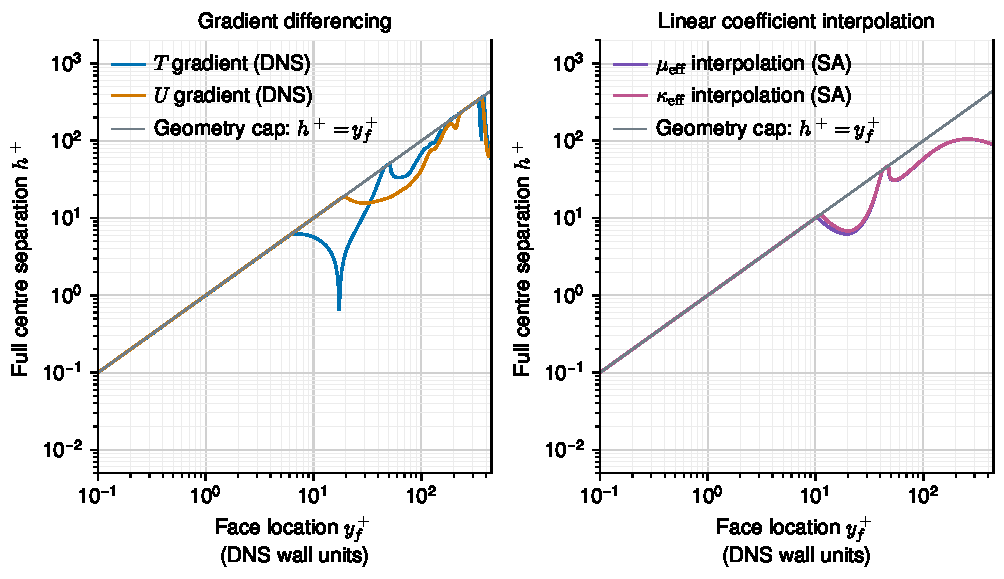
\includegraphics[width=\linewidth]{07_Error_Isolation_Results/Figures/Recon/M6Tw025_3pct_envelope.pdf}
    \caption{M6Tw025 spacing limits at a $3\%$ local component-error tolerance. The allowable full centre separation $h^+$ is plotted against internal-face position $y_f^+$ for centred differencing of DNS temperature and velocity (left) and linear interpolation of wall-resolved SA effective transport (right). Each limit is the first tolerance crossing evaluated on cubic profile reconstructions, capped by the adopted geometric condition $h^+\leq y_f^+$. Both coordinates use DNS wall units.}
    \label{fig:WF:M6Tw025-3pct-envelope-all-quantities}
\end{figure}

To satisfy all four component criteria of Figure~\ref{fig:WF:M6Tw025-3pct-envelope-all-quantities} simultaneously, the allowable spacing is their minimum at each face position, further limited by profile support and the geometric cap. Figure~\ref{fig:WF:M6Tw025-3pct-envelope-combined} is the resulting $3\%$ envelope. It converts the separate operator restrictions into a single wall-normal spacing requirement. Near the cold-wall temperature maximum, its large separation from $h^+=y_f^+$ quantifies why the conventional coarse stencil is inadequate and how much smaller the centre separation must be to avoid excessive errors. It must be emphasized that this is a local operator criterion, not a $3\%$ error bound on the wall heat-flux or shear stress. Additionally these four component errors can add constructively or destructively, so the combined envelope is not a direct error estimate, but it limits their individual contributions.

\begin{figure}[H]
    \centering
    % Figure provenance (WSL; absolute paths):
    %   Figure: /home/mgnadlinger/Xue_et_al/flat_plate/M6Tw025/opt_mesh/spacing_limits/M6Tw025_3pct_limits_only_font80.png
    %   Python scripts:
    %     /home/mgnadlinger/Xue_et_al/flat_plate/M6Tw025/opt_mesh/scripts/plot_cubic_limits_font80.py
    %     /home/mgnadlinger/Xue_et_al/flat_plate/M6Tw025/opt_mesh/scripts/plot_analysis.py
    %   Data / simulation roots (high-level):
    %     /home/mgnadlinger/Xue_et_al/flat_plate/M6Tw025/opt_mesh/spacing_limits
    %     /home/mgnadlinger/Xue_et_al/flat_plate/M6Tw025/opt_mesh/reference
    %     /home/mgnadlinger/Xue_et_al/flat_plate/M6Tw025/Digitizations
    %     /home/mgnadlinger/Xue_et_al/flat_plate/M6Tw025/Li_SA/SA_Prt0p9_baseline
    %   Note: Combined envelope is plotted from the finite-stencil limit tables generated by plot_analysis.py.
    % End figure provenance.
    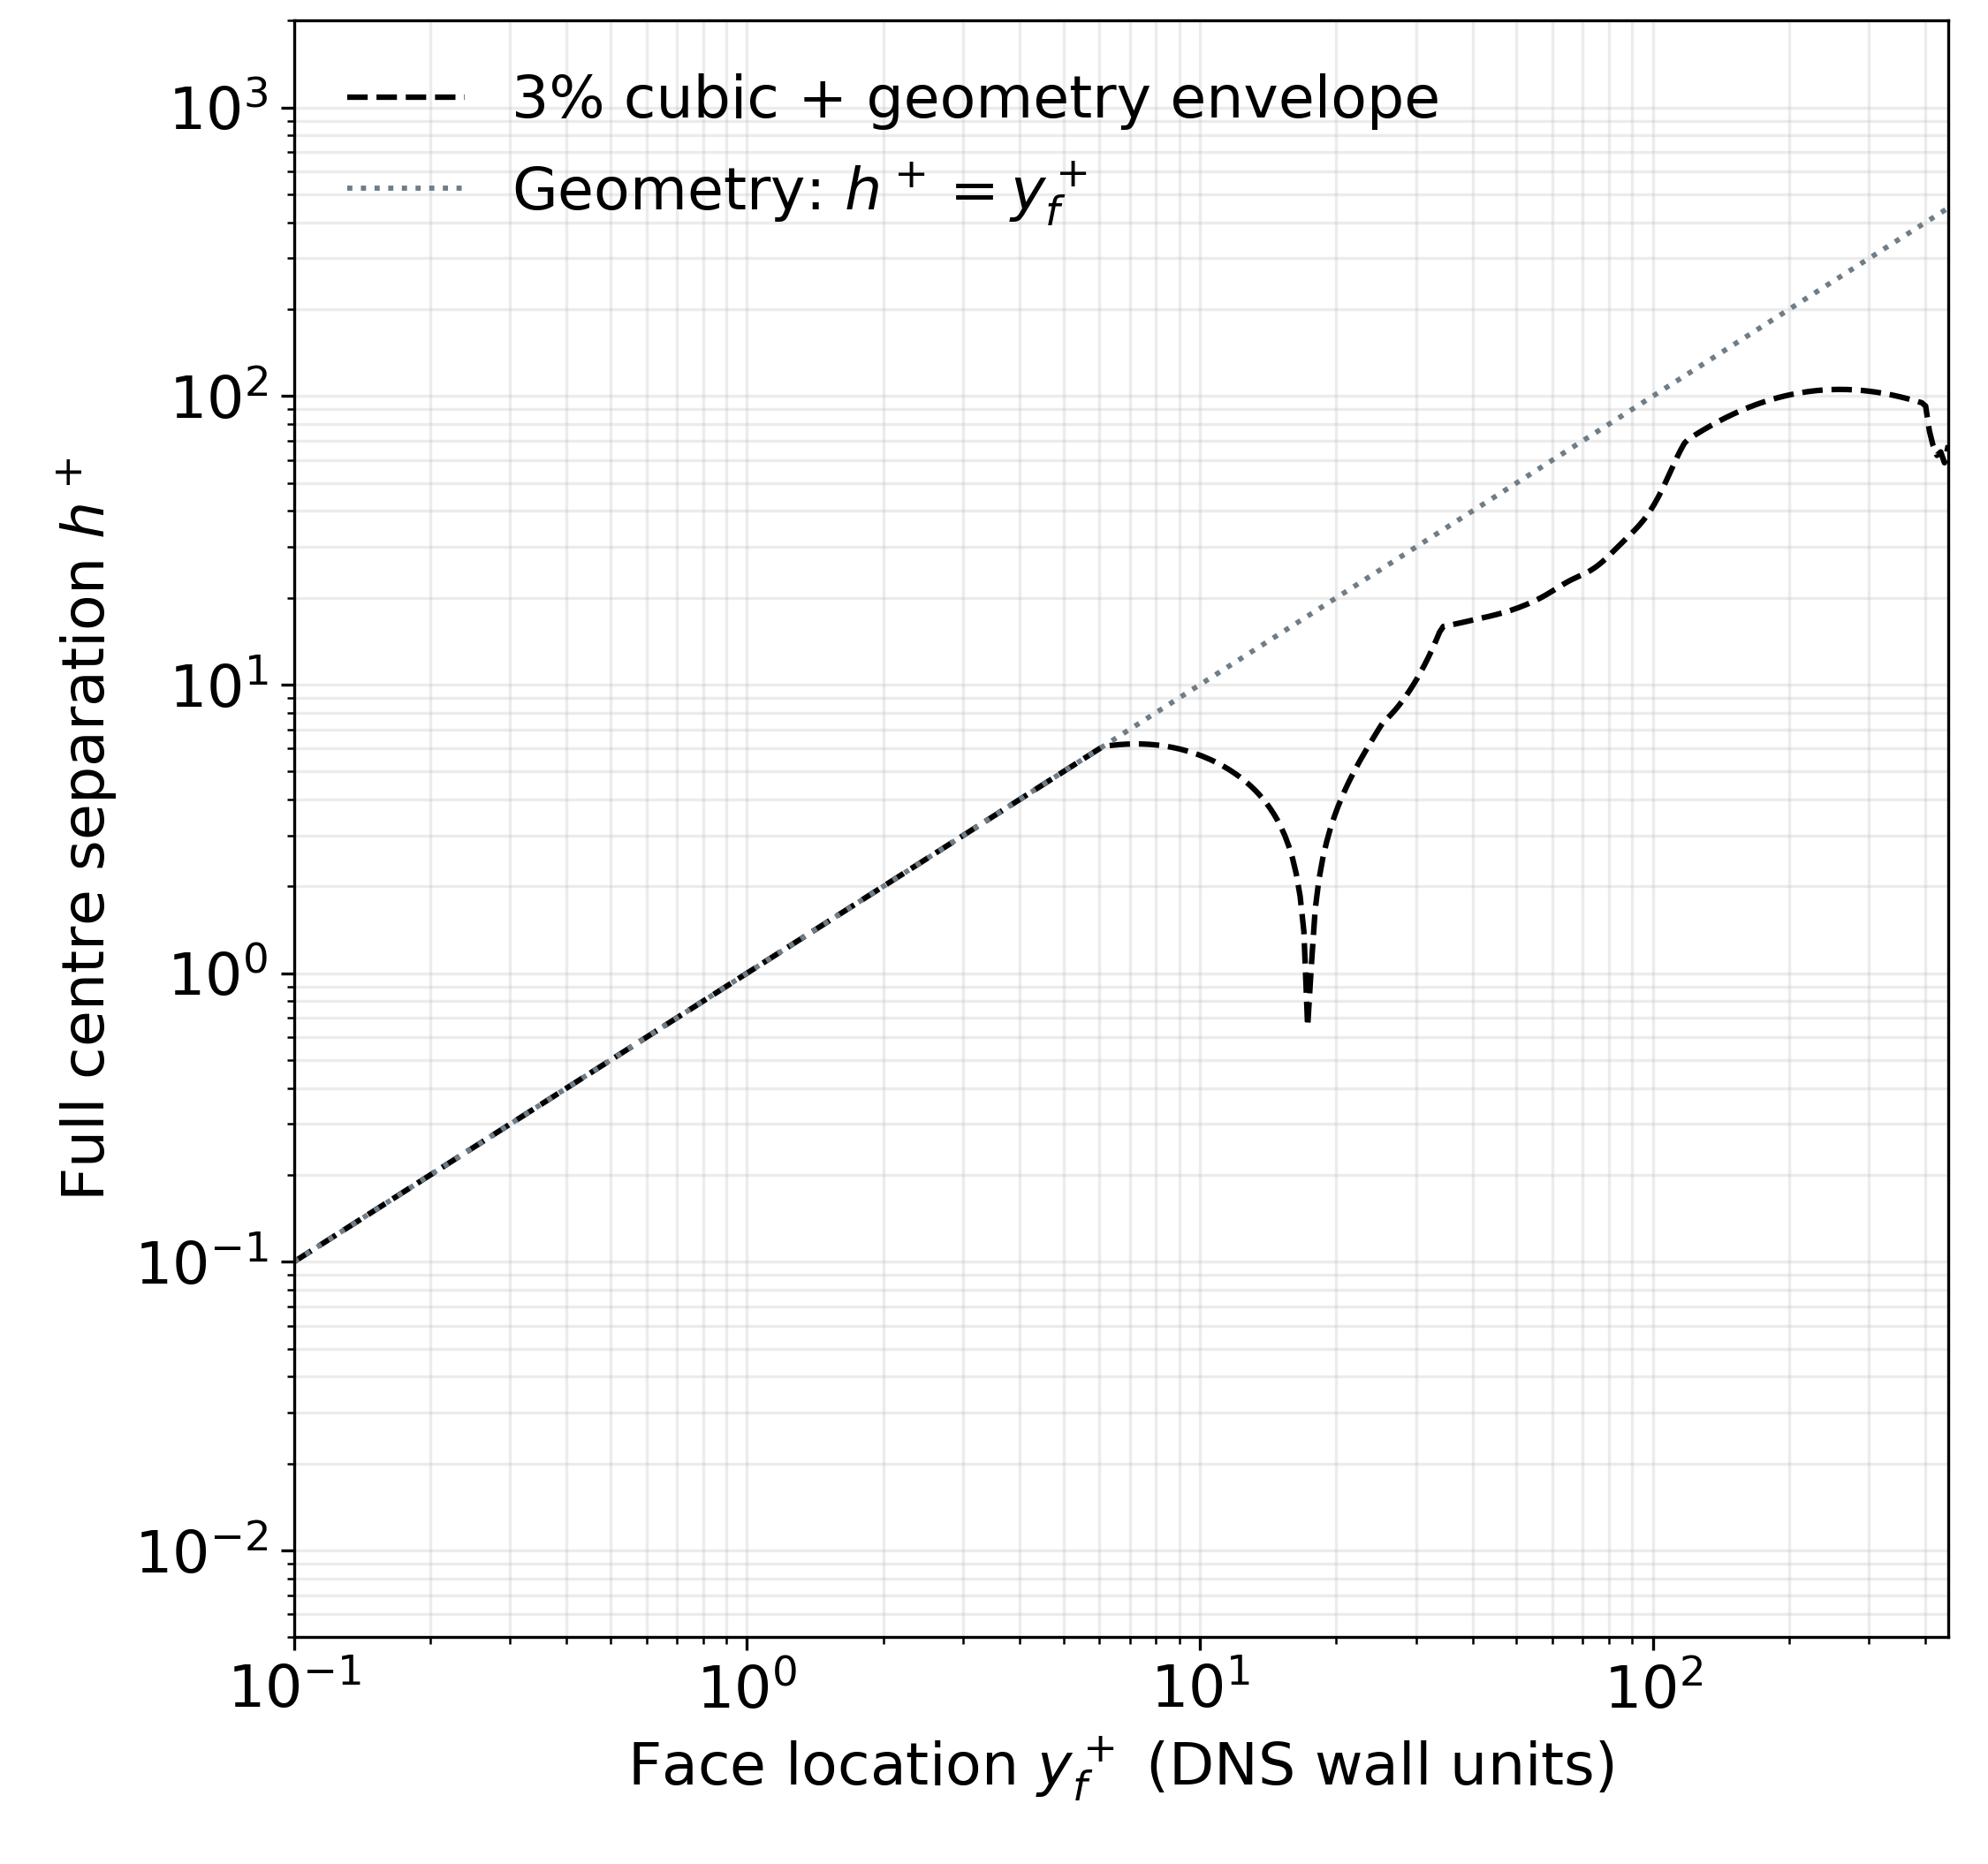
\includegraphics[width=0.7\linewidth,height=.62\textheight,keepaspectratio]{07_Error_Isolation_Results/Figures/WallFunctions/M6Tw025_3pct_envelope.png}
    \caption{Combined M6Tw025 spacing envelope for a $3\%$ component-error tolerance: the minimum of the four cubic-reference limits in Figure~\ref{fig:WF:M6Tw025-3pct-envelope-all-quantities}, profile support and the geometric cap $h^+=y_f^+$. The restrictive region near the temperature maximum requires substantially smaller centre separation than a conventional coarse stencil.}
    \label{fig:WF:M6Tw025-3pct-envelope-combined}
\end{figure}

Repeating the same analysis with $\epsilon=0.10$ gives Figure~\ref{fig:WF:M6Tw025-10pct-envelope-combined}. The restrictive minimum persists in the buffer region, whereas substantially larger spacings are admitted farther into the logarithmic region. Around $y_f^+\approx150$, the envelope reaches the geometric cap. Meaning a conventional symmetric coarse wall-function mesh stencil can locally satisfy the $10\%$ component tolerance and supports the finding discussed in Section~\ref{subsec:comparative:zpg:conventional-mesh}, that these log-layer regions are the ones used in the papers of Li et al. and Griffin et al. for validation purposes.

\begin{figure}[H]
    \centering
    % Figure provenance (WSL; absolute paths):
    %   Figure: /home/mgnadlinger/Xue_et_al/flat_plate/M6Tw025/opt_mesh/spacing_limits/M6Tw025_10pct_limits_only_font80.png
    %   Python scripts:
    %     /home/mgnadlinger/Xue_et_al/flat_plate/M6Tw025/opt_mesh/scripts/plot_cubic_limits_font80.py
    %     /home/mgnadlinger/Xue_et_al/flat_plate/M6Tw025/opt_mesh/scripts/plot_analysis.py
    %   Data / simulation roots (high-level):
    %     /home/mgnadlinger/Xue_et_al/flat_plate/M6Tw025/opt_mesh/spacing_limits
    %     /home/mgnadlinger/Xue_et_al/flat_plate/M6Tw025/opt_mesh/reference
    %     /home/mgnadlinger/Xue_et_al/flat_plate/M6Tw025/Digitizations
    %     /home/mgnadlinger/Xue_et_al/flat_plate/M6Tw025/Li_SA/SA_Prt0p9_baseline
    %   Note: Combined envelope is plotted from the finite-stencil limit tables generated by plot_analysis.py.
    % End figure provenance.
    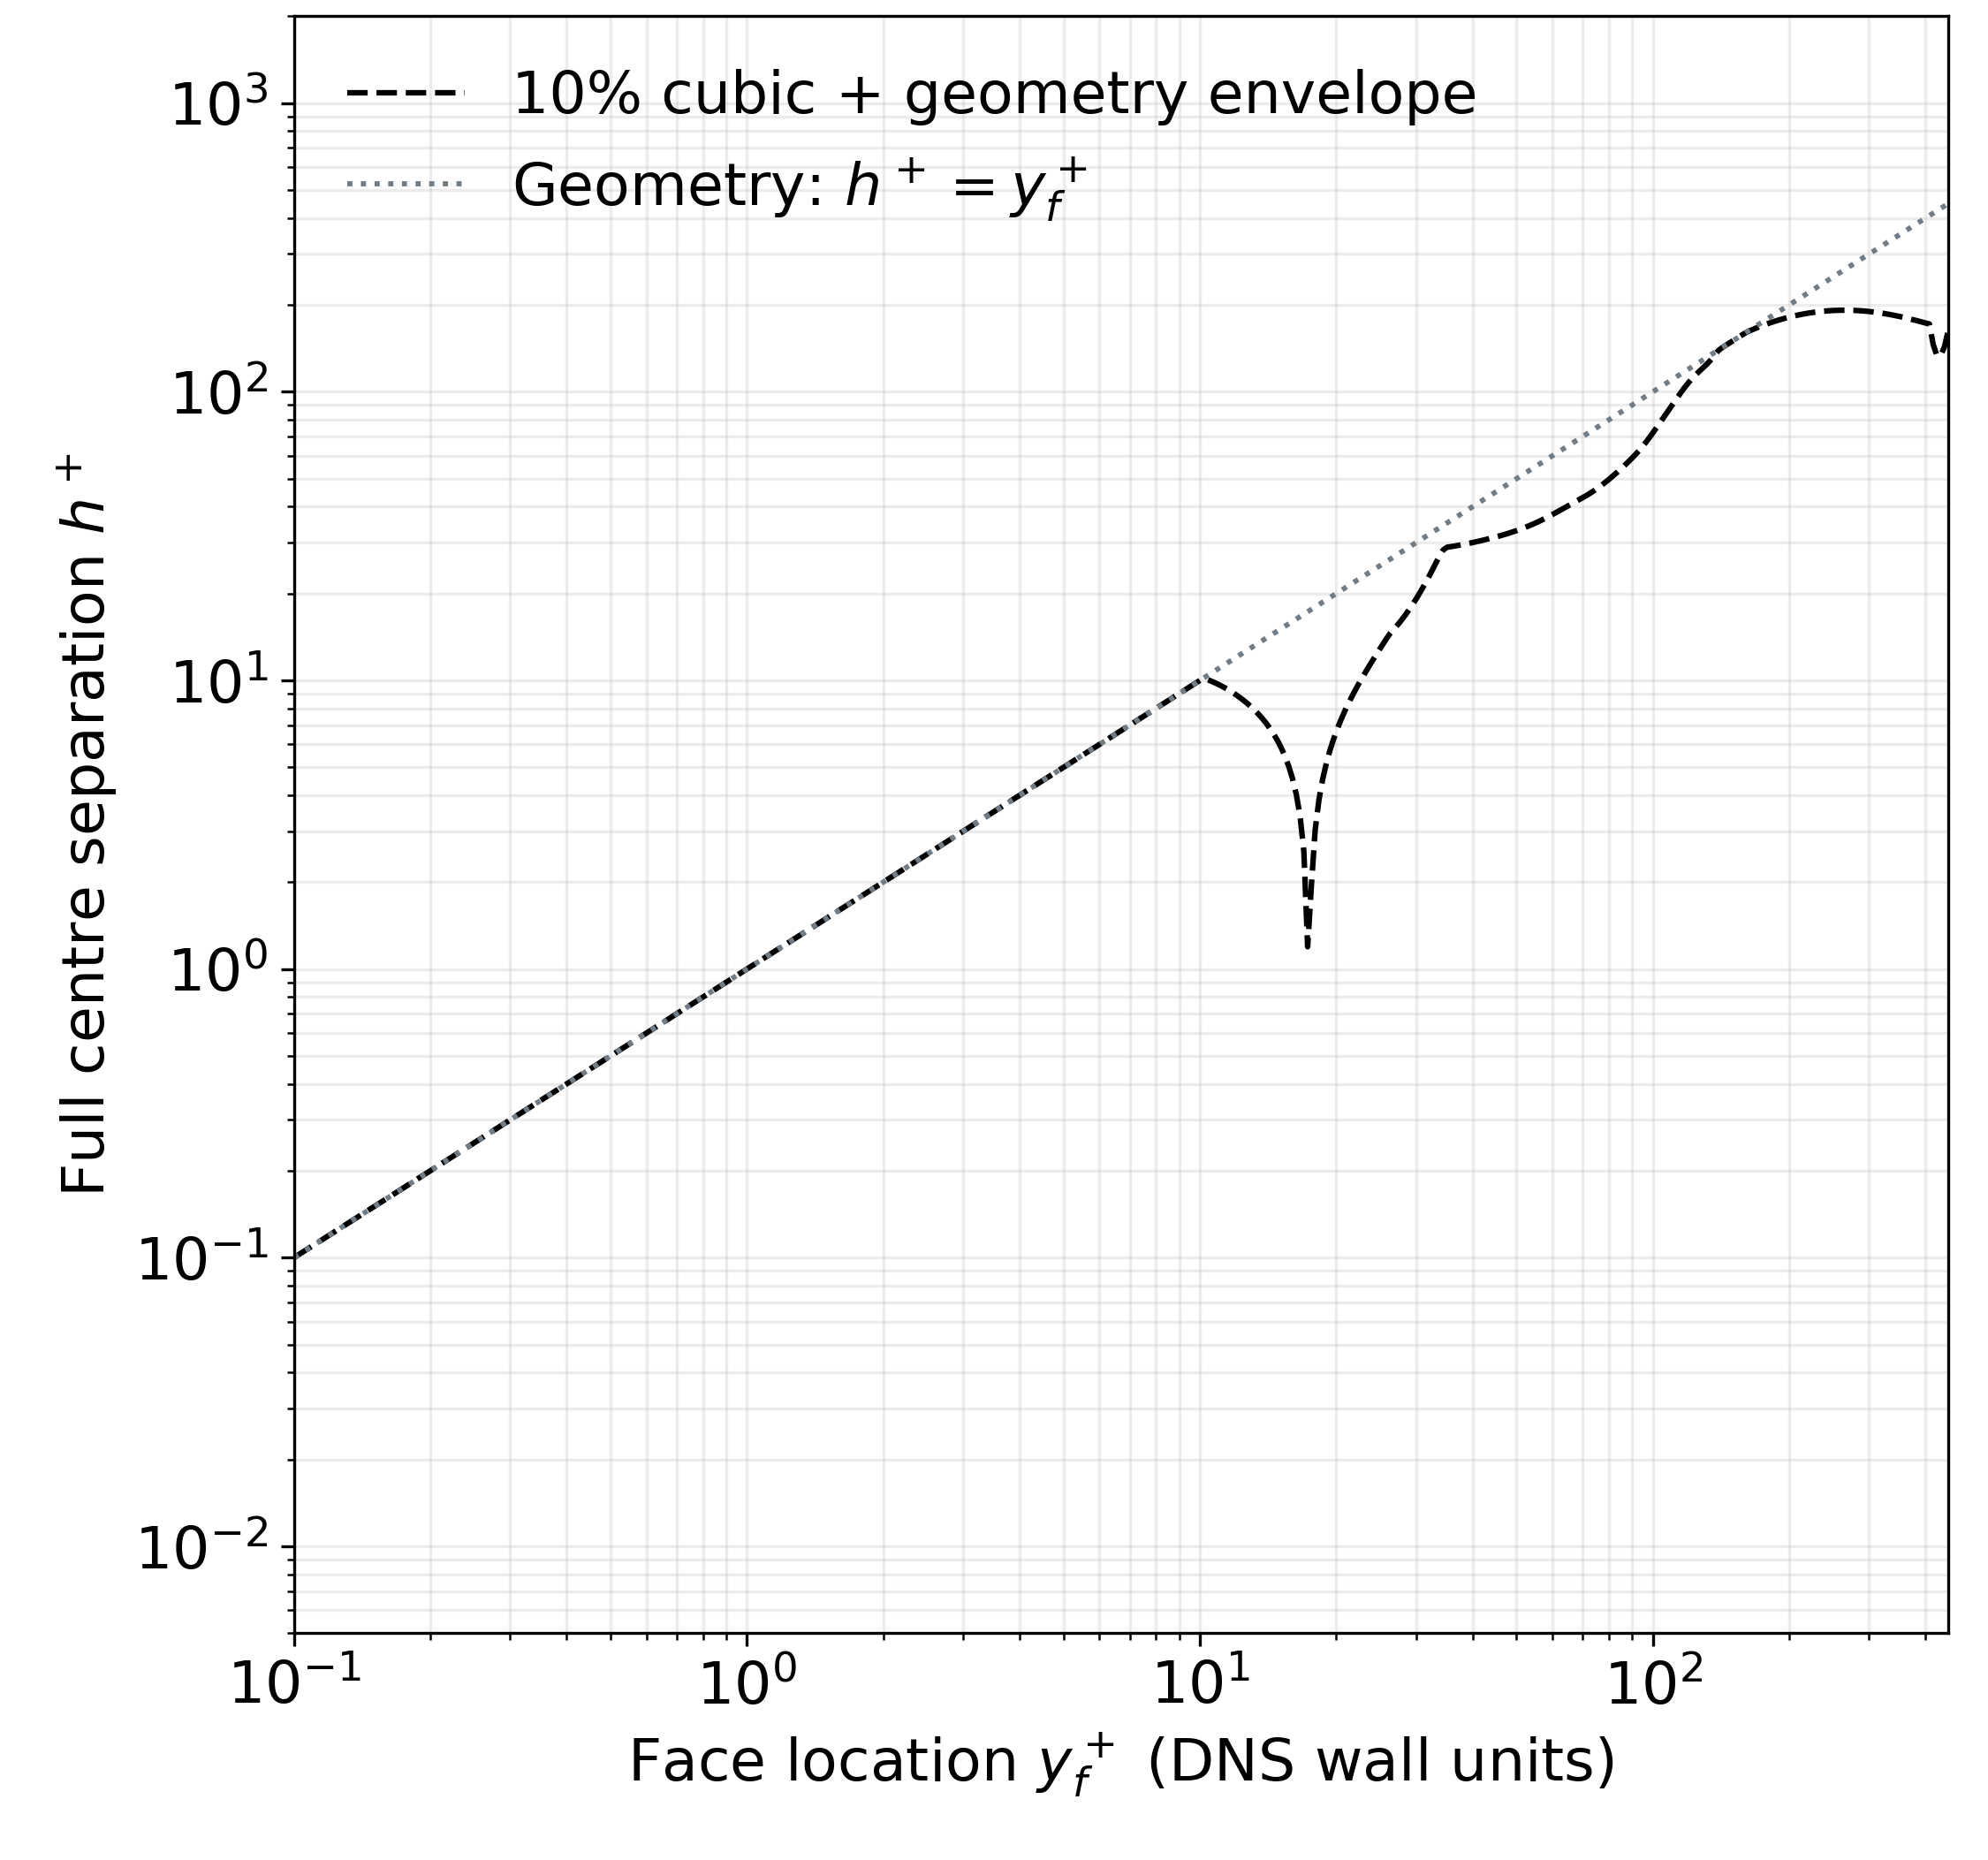
\includegraphics[width=0.7\linewidth,height=.62\textheight,keepaspectratio]{07_Error_Isolation_Results/Figures/WallFunctions/M6Tw025_10pct_envelope.png}
    \caption{Combined M6Tw025 spacing envelope with the local component-error tolerance relaxed to $10\%$. The restrictive minimum near the temperature maximum persists, while larger spacings are permitted farther outward. Around $y_f^+\approx150$, the envelope reaches the geometric cap and locally admits the conventional symmetric first-face stencil of Figure~\ref{fig:WF:exemplaray_y+10_mesh}. This is a local operator criterion, rather than a $10\%$ bound on CFD wall quantities.}
    \label{fig:WF:M6Tw025-10pct-envelope-combined}
\end{figure}

The physical reason on why this meshing restriction only arises now in hypersonic cold-wall boundary layers, and not in the subsonic or adiabatic-wall hypersonic cases can be seen in the comparative Figures~\ref{fig:WF:dns-velocity-profiles-linear} and~\ref{fig:WF:dns-temperature-profiles-linear}. There the M6Tw025 case is compared to the near-adiabatic M6Tw076 case and a transonic cold-wall case \textit{C09} of \cite{iwatani2025subharmonic}. Neither of the latter two cases show a pronounced temperature peak, and therefore the curvature variation is much less.

\begin{figure}[H]
    \centering
    % Figure provenance (paths relative to the thesis workspace root):
    % Original vector export: tmp/boundary_layer_profile_comparison/velocity_profiles_linear.pdf
    % Generating script: tmp/boundary_layer_profile_comparison/plot_linear_profiles.py
    % Shared data loading and styles: tmp/boundary_layer_profile_comparison/plot_profiles.py
    % Retained DNS files and preprocessing: tmp/boundary_layer_profile_comparison/raw/
    % Scaling checks and source URLs: tmp/boundary_layer_profile_comparison/source_notes.txt
    % Same DNS samples and normalizations as fig:background:dns-velocity-profiles:
    % Zhang, Duan and Choudhari (2018), DOI 10.2514/1.J057296;
    % Iwatani, Asada and Kawai (2025), DOI 10.1016/j.ijheatfluidflow.2025.109896.
    % C09: X=11, inferred velocity factor 0.8, conventional y+ reconstructed
    % from archived skin friction and wall properties, as documented in the background.
    % Linear y+ from 0 to 1200 includes all native samples and the wall points.
    % Copied without cropping or resizing the source PDF.
    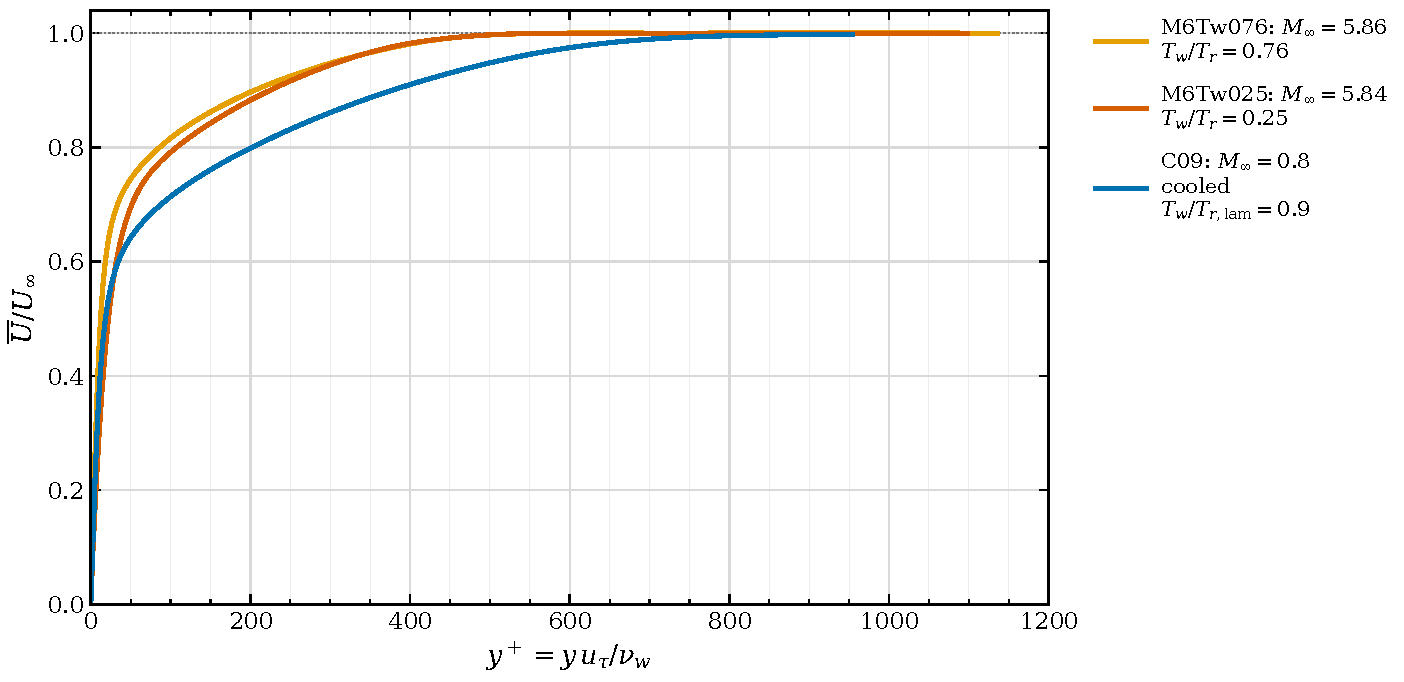
\includegraphics[width=\linewidth]{07_Error_Isolation_Results/Figures/Recon/velocity_profiles_linear.pdf}
    \caption[DNS velocity profiles on a linear wall-normal coordinate]{Freestream-normalized DNS velocity profiles for M6Tw076, M6Tw025 and C09, using the same data and normalization as Figure~\ref{fig:background:dns-velocity-profiles}, now plotted against linear \(y^+\). The native wall points at \(y^+=0\) are included.}
    \label{fig:WF:dns-velocity-profiles-linear}
\end{figure}

\begin{figure}[H]
    \centering
    % Figure provenance (paths relative to the thesis workspace root):
    % Original vector export: tmp/boundary_layer_profile_comparison/temperature_profiles_linear.pdf
    % Generating scripts, retained source data and scaling conventions:
    % as for fig:WF:dns-velocity-profiles-linear immediately above.
    % Native Reynolds-mean T/Tinf values are retained for all three cases.
    % Same thermal profiles as fig:background:dns-temperature-profiles;
    % linear y+ from 0 to 1200, including the native wall points, also in the C09 inset.
    % Copied without cropping or resizing the source PDF.
    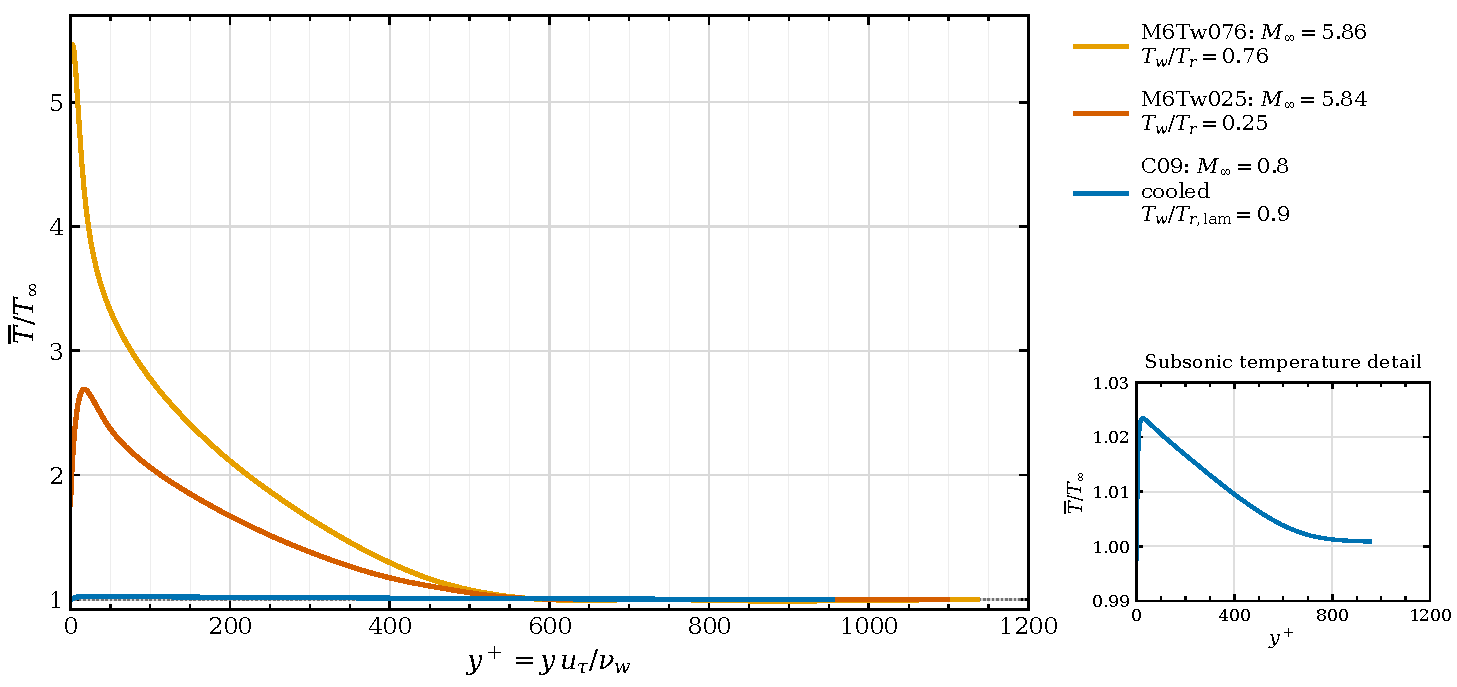
\includegraphics[width=\linewidth]{07_Error_Isolation_Results/Figures/Recon/temperature_profiles_linear.pdf}
    \caption[Linear thermal profiles and curvature variation near the cold-wall peak]{DNS temperature profiles from Figure~\ref{fig:background:dns-temperature-profiles}, shown on a linear \(y^+\) axis to better visualize the pronounced change in curvature associated with the hypersonic cold-wall M6Tw025 temperature peak. Since \(y^+\) is proportional to physical \(y\) within each case, this view connects the thermal-profile structure to finite stencil spacing and the reconstruction error illustrated by the secant--tangent comparison in Figure~\ref{fig:WF:exemplaray_y+10_reconstruction_error}. The C09 inset uses a separate vertical scale.}
    \label{fig:WF:dns-temperature-profiles-linear}
\end{figure}

All in all, the above analysis shows that the conventional coarse wall-function mesh stencil, paired with second-order accurate schemes, is not sufficient to resolve the internal-face transport in hypersonic cold-wall boundary layers. The pronounced temperature peak causes a large change in curvature, which in turn requires a much smaller centre separation than the conventional coarse wall-function mesh stencil provides. This novel mesh requirement is thus only dependant on the boundary layer profile and numerical schemes, in turn this requirement also applies to wall-resolved runs. In other words, the wall-functions can be understood as just a different heat-flux and shear stress relation than the convential linear correlation between the first off-wall cell cetner to the wall, as described for wall-resolved RANS in Equation~\eqref{eq:q_w_openFOAM_math}. But with the very low first-cell requirement of these wall-resolved runs on hypersonic cold-walls (i.e. the first-cell acoustic Reynolds number must be below 1 as discussed in Section~\ref{sec:evaluation:mesh-families-yplus}), only very extreme growth rates of the boundary layer mesh may run into any appreciable internal-face transport error, thus it remained undiscussed so far.
\par\medskip

The following section will show how proof this hypothesis by isolating these discretization errors through constructing boundary layer-informed meshes that satisfy the above discussed $3\%$ criterion.

\subsection{Wall functions on boundary layer-informed meshes}
\label{subsec:comparative:zpg:informed-mesh}

To test the above discussed error due to spatial discretization in CFD, families of boundary layer-informed meshes are constructed for prescribed wall-function sampling positions. This allows the wall-function sample to be swept over the whole $y^+$ range similar to the wall-closures a-priori analysis in Section~\ref{subsec:erriso:apriori-solver} and conventional mesh CFD runs in Figures~\ref{fig:WF:Li-LowHM3_conventional_mesh}--\ref{fig:WF:Griffin-M6Tw025_conventional_mesh}, while the internal-face spacing is controlled by the above discussed $3\%$ criterion. This arrangement reduces the coupling between moving the wall-function sample and the boundary layer spatial discretization.
\par\medskip

Figures~\ref{fig:WF:LowHM3-3pct-mesh-sweep} and~\ref{fig:WF:M6Tw025-3pct-mesh-sweep} show the resulting families for the M6Tw025 and LowH\_M3 case respectivly. The dotted and dashed lines are taken and constructed as described in the boundary layer analysis Section~\ref{subsec:comparative:zpg:mesh-criterion} above - specifically for the M6Two025 case, the Figure~\ref{fig:WF:M6Tw025-3pct-mesh-sweep} dashed and dotted lines are the same as in the Figure~\ref{fig:WF:M6Tw025-3pct-envelope-combined}. For the construction of the mesh families (see Figures~\ref{fig:WF:LowHM3-3pct-mesh-sweep} and~\ref{fig:WF:M6Tw025-3pct-mesh-sweep} right plots), a desired wall-function sampling height is prescribed and the internal-face spacing around it is then grown up until the allowable  discretization error of e.g. $3\%$ against the known profile is reached. This is continued until the whole boundary layer is covered. The resulting meshes are not a bound on the total CFD error or a proof of a globally optimal meshing, but aim to provide an isolation from this error source. The generated meshes are subsequently re-checked against the known boundary layer profiles, using their actual, generally unsymmetric, centre-to-face distances to ensure the desired spacing criterion is really satisfied.

\begin{figure}[H]
    \centering
    % Figure provenance (WSL; absolute paths):
    %   Figure: /home/mgnadlinger/WF_validation/LowH_M3/opt_meshes/marching_design/LowH_M3_mesh_sweep_3pct.png
    %   Python script:
    %     /home/mgnadlinger/WF_validation/LowH_M3/opt_meshes/marching_design/plot_mesh_report.py
    %   Data / simulation roots (high-level):
    %     /home/mgnadlinger/WF_validation/LowH_M3/opt_meshes/marching_design/3pct
    %     /home/mgnadlinger/WF_validation/LowH_M3/opt_meshes/marching_design/reference
    %     /home/mgnadlinger/WF_validation/LowH_M3/opt_meshes/Li_fitted_3pct_minCells_SA
    %     /home/mgnadlinger/WF_validation/LowH_M3/wall_resolved/SA/LowH_M3
    %   Note: Mesh-design report uses the frozen wall-resolved SA reference and the written fitted-Li mesh
    %     family.
    % End figure provenance.
    %   Print-size typography: regenerated at 170 mm width with 10 pt text; exact source data
    %     and local plotting script retained in Figures/WallFunctions/mesh_sweep_font_sources/.
    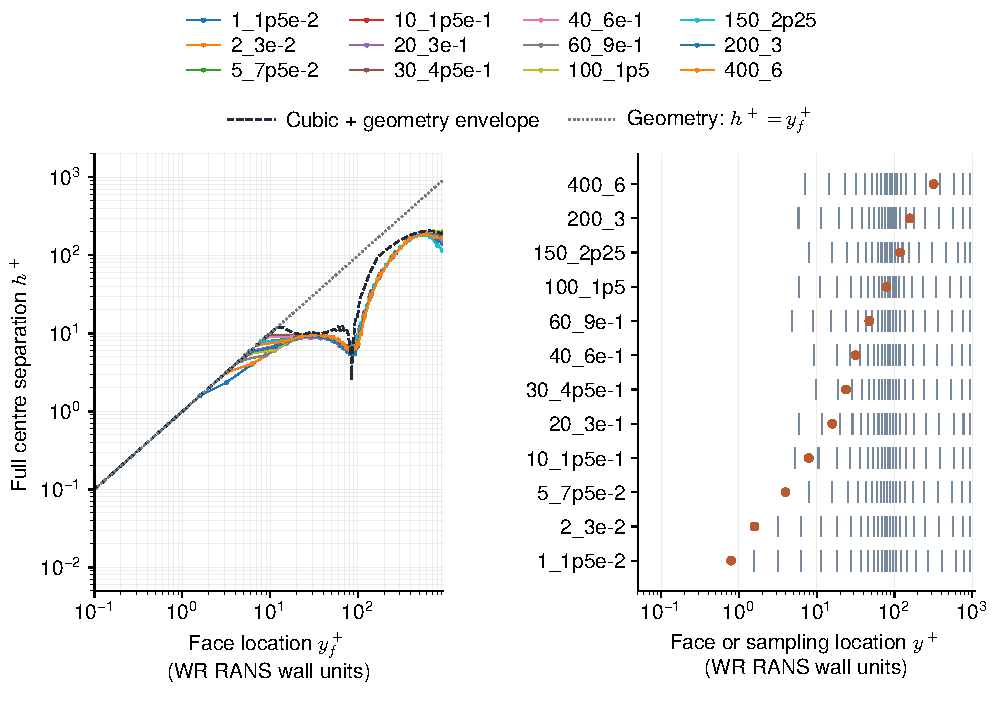
\includegraphics[width=\linewidth]{07_Error_Isolation_Results/Figures/WallFunctions/LowHM3_mesh_sweep_3pct.pdf}
    \caption{Boundary layer-informed $3\%$ spatial discretization error mesh family for LowH\_M3. The naming of the mesh families follows the structure \textit{desired wall-function sampling point in $y^+$}\_\textit{desired wall-function sampling point in millimetres}. Left: Black dotted and dashed lines represent the envelope stemming from the boundary layer analysis as described in Section~\ref{subsec:comparative:zpg:mesh-criterion}. The colourfull lines show the new boundary layer-informed meshes' actual spatial discretization error against the known boundary layer profiles, with all of them consistently staying below the $3\%$ envelope. Right: The actual mesh design (blue lines represent the position of the cell faces) and wall-function sampling centres (orange) are shown, with the pronounced clustering around the $y^+\approx85$ where the temperature peak sits for this case.} 
    \label{fig:WF:LowHM3-3pct-mesh-sweep}
\end{figure}

\begin{figure}[H]
    \centering
    % Figure provenance (WSL; absolute paths):
    %   Figure: /home/mgnadlinger/Xue_et_al/flat_plate/M6Tw025/opt_mesh/spacing_limits/M6Tw025_mesh_sweep_3pct.png
    %   Python script:
    %     /home/mgnadlinger/Xue_et_al/flat_plate/M6Tw025/opt_mesh/scripts/plot_analysis.py
    %   Data / simulation roots (high-level):
    %     /home/mgnadlinger/Xue_et_al/flat_plate/M6Tw025/opt_mesh/searches/3pct
    %     /home/mgnadlinger/Xue_et_al/flat_plate/M6Tw025/opt_mesh/Li_3pct_SA
    %     /home/mgnadlinger/Xue_et_al/flat_plate/M6Tw025/opt_mesh/spacing_limits
    %     /home/mgnadlinger/Xue_et_al/flat_plate/M6Tw025/opt_mesh/reference
    %     /home/mgnadlinger/Xue_et_al/flat_plate/M6Tw025/Digitizations
    %     /home/mgnadlinger/Xue_et_al/flat_plate/M6Tw025/Li_SA/SA_Prt0p9_baseline
    %   Note: Source report identifies this as the ordinary-Li mesh family.
    % End figure provenance.
    %   Print-size typography: regenerated at 170 mm width with 10 pt text; exact source data
    %     and local plotting script retained in Figures/WallFunctions/mesh_sweep_font_sources/.
    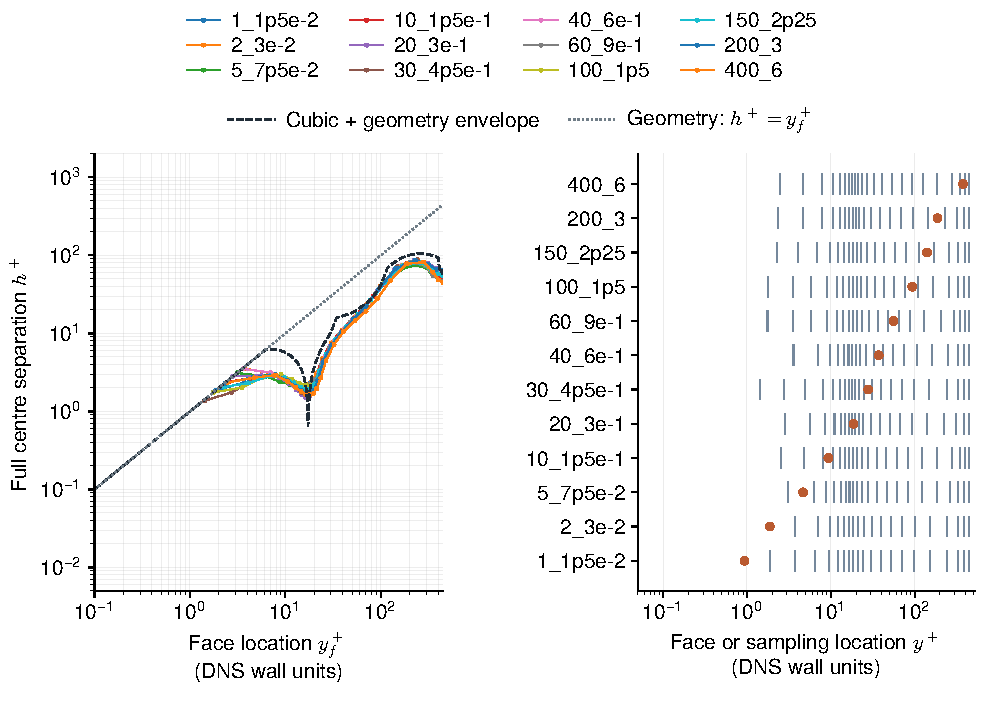
\includegraphics[width=\linewidth]{07_Error_Isolation_Results/Figures/WallFunctions/M6Tw025_mesh_sweep_3pct.pdf}
    \caption{Boundary layer-informed $3\%$ spatial discretization error mesh family for M6Tw025. The naming of the mesh families follows the structure \textit{desired wall-function sampling point in $y^+$}\_\textit{desired wall-function sampling point in millimetres}. Left: Black dotted and dashed lines represent the envelope stemming from the boundary layer analysis as described in Section~\ref{subsec:comparative:zpg:mesh-criterion}. The colourfull lines show the new boundary layer-informed meshes' actual spatial discretization error against the known boundary layer profiles, with all of them consistently staying below the $3\%$ envelope. Right: The actual mesh design (blue lines represent the position of the cell faces) and wall-function sampling centres (orange) are shown, with the pronounced clustering around the $y^+\approx18$ where the temperature peak sits for this case.}
    \label{fig:WF:M6Tw025-3pct-mesh-sweep}
\end{figure}

Figure~\ref{fig:WF:3pct-bl-informed-mesh-CFD-results} presents the CFD sweeps on these meshes. The abscissa is now the wall-function's sample location $y_s^+$, rather than necessarily the physical first-cell $y_1^+$. The reader is encouraged to look at the a-priori analysis, conventional coarase wall-function mesh CFD and herein presented boundary layer-informed mesh CFD results side by side for the four investigated combionations of Li wall function and Griffin wall function on the LowH\_M3 and M6Tw025 case (e.g. for the Li wall function on the LowH\_M3 case, see Figures~\ref{fig:wall-closure:a-priori-Li-LowHM3},~\ref{fig:WF:Li-LowHM3_conventional_mesh} and~\ref{fig:WF:3pct-bl-informed-mesh-CFD-results} top).
\par\medskip

It is immediatly apparant that the boundary layer-informed meshes follow the general error trend of the a-priori found closure error, significantly better than the conventional coarse wall-function meshes. The pronounced overshoot in the buffer layer that the conventional mesh exhibits in Figure~\ref{fig:WF:Li-LowHM3_conventional_mesh} is removed and the boundary layer-informed meshes in Figure~\ref{fig:WF:3pct-bl-informed-mesh-CFD-results} (top) show significantly closer trend to the a-priori results of Figure~\ref{fig:wall-closure:a-priori-Li-LowHM3}. Also indicative is, that Figure~\ref{fig:WF:Li-LowHM3_conventional_mesh} from $y^+\approx2$ onwards deviated from the wall-resolved baseline, whereas the boundary layer-informed meshes in Figure~\ref{fig:WF:3pct-bl-informed-mesh-CFD-results} (top) follow the a-priori in Figure~\ref{fig:wall-closure:a-priori-Li-LowHM3}, of effectly zero error, up to the same $y^+\approx10$.
\par\medskip

Because of error addition and cancellation, the wall-function CFD results on the boundary layer-informed meshes do not exactly match the quantiataive errors of the a-priori analysis. Arguably an even finer boundary layer-informed mesh with $\epsilon_max \le 0.1\%$ could be designed to further isolate the discretization errors, this highlights how big of an impact even these small discretization errors can have. For comparing the M6Tw025 cases, one should also keep in mind, that an additonal uncertainty arises in the discovered fact, that the turbulence model is not capable to reproduce the DNS temperature peak, as discussed in Section~\ref{subsec:comparative:zpg:wr-profiles} and investigated implications in Section~\ref{subsec:erriso:rans-profile-influence}.
\par\medskip

The highest sampling positions require particular caution. The LowH\_M3 Li curve rises markedly at its outermost sample, where inner-layer and approximately constant-stress assumptions become less suitable as discussed in the a-prori analysis in Section~\ref{subsec:comparative:zpg:apriori-mesh}. This point does not establish a general acceptable upper $y_s^+$, since the relevant boundary layer region and the closure's usable range are case dependent.
\par\medskip

From the analysis there is a strong conclusion from the CFD results of the herin used boundary layer-informed meshes vs. the previous conventional meshes, that the large error in the buffer layer and lower log-layer is driven by the spatial discretization error discussed as hypthesized.

\begin{figure}[H]
    \centering
    % Figure provenance (WSL; absolute paths):
    %   Figure: /home/mgnadlinger/WF_validation/LowH_M3/validation/outputs/plots/opt_mesh/li_3pct_mincells_sa_dns_station_relative_error.png
    %   Python scripts:
    %     /home/mgnadlinger/WF_validation/LowH_M3/validation/scripts/plot_opt_mesh_wall_flux_sweeps.py
    %     /home/mgnadlinger/WF_validation/LowH_M3/validation/scripts/plot_wall_flux_sweeps.py
    %   Data / simulation roots (high-level):
    %     /home/mgnadlinger/WF_validation/LowH_M3/opt_meshes/Li_3pct_minCells_SA
    %     /home/mgnadlinger/WF_validation/LowH_M3/wall_resolved/SA/LowH_M3
    %     /home/mgnadlinger/WF_validation/LowH_M3/Digitizations
    %   Note: Thesis image removes the 128-pixel title strip from the source export.
    % End figure provenance.
    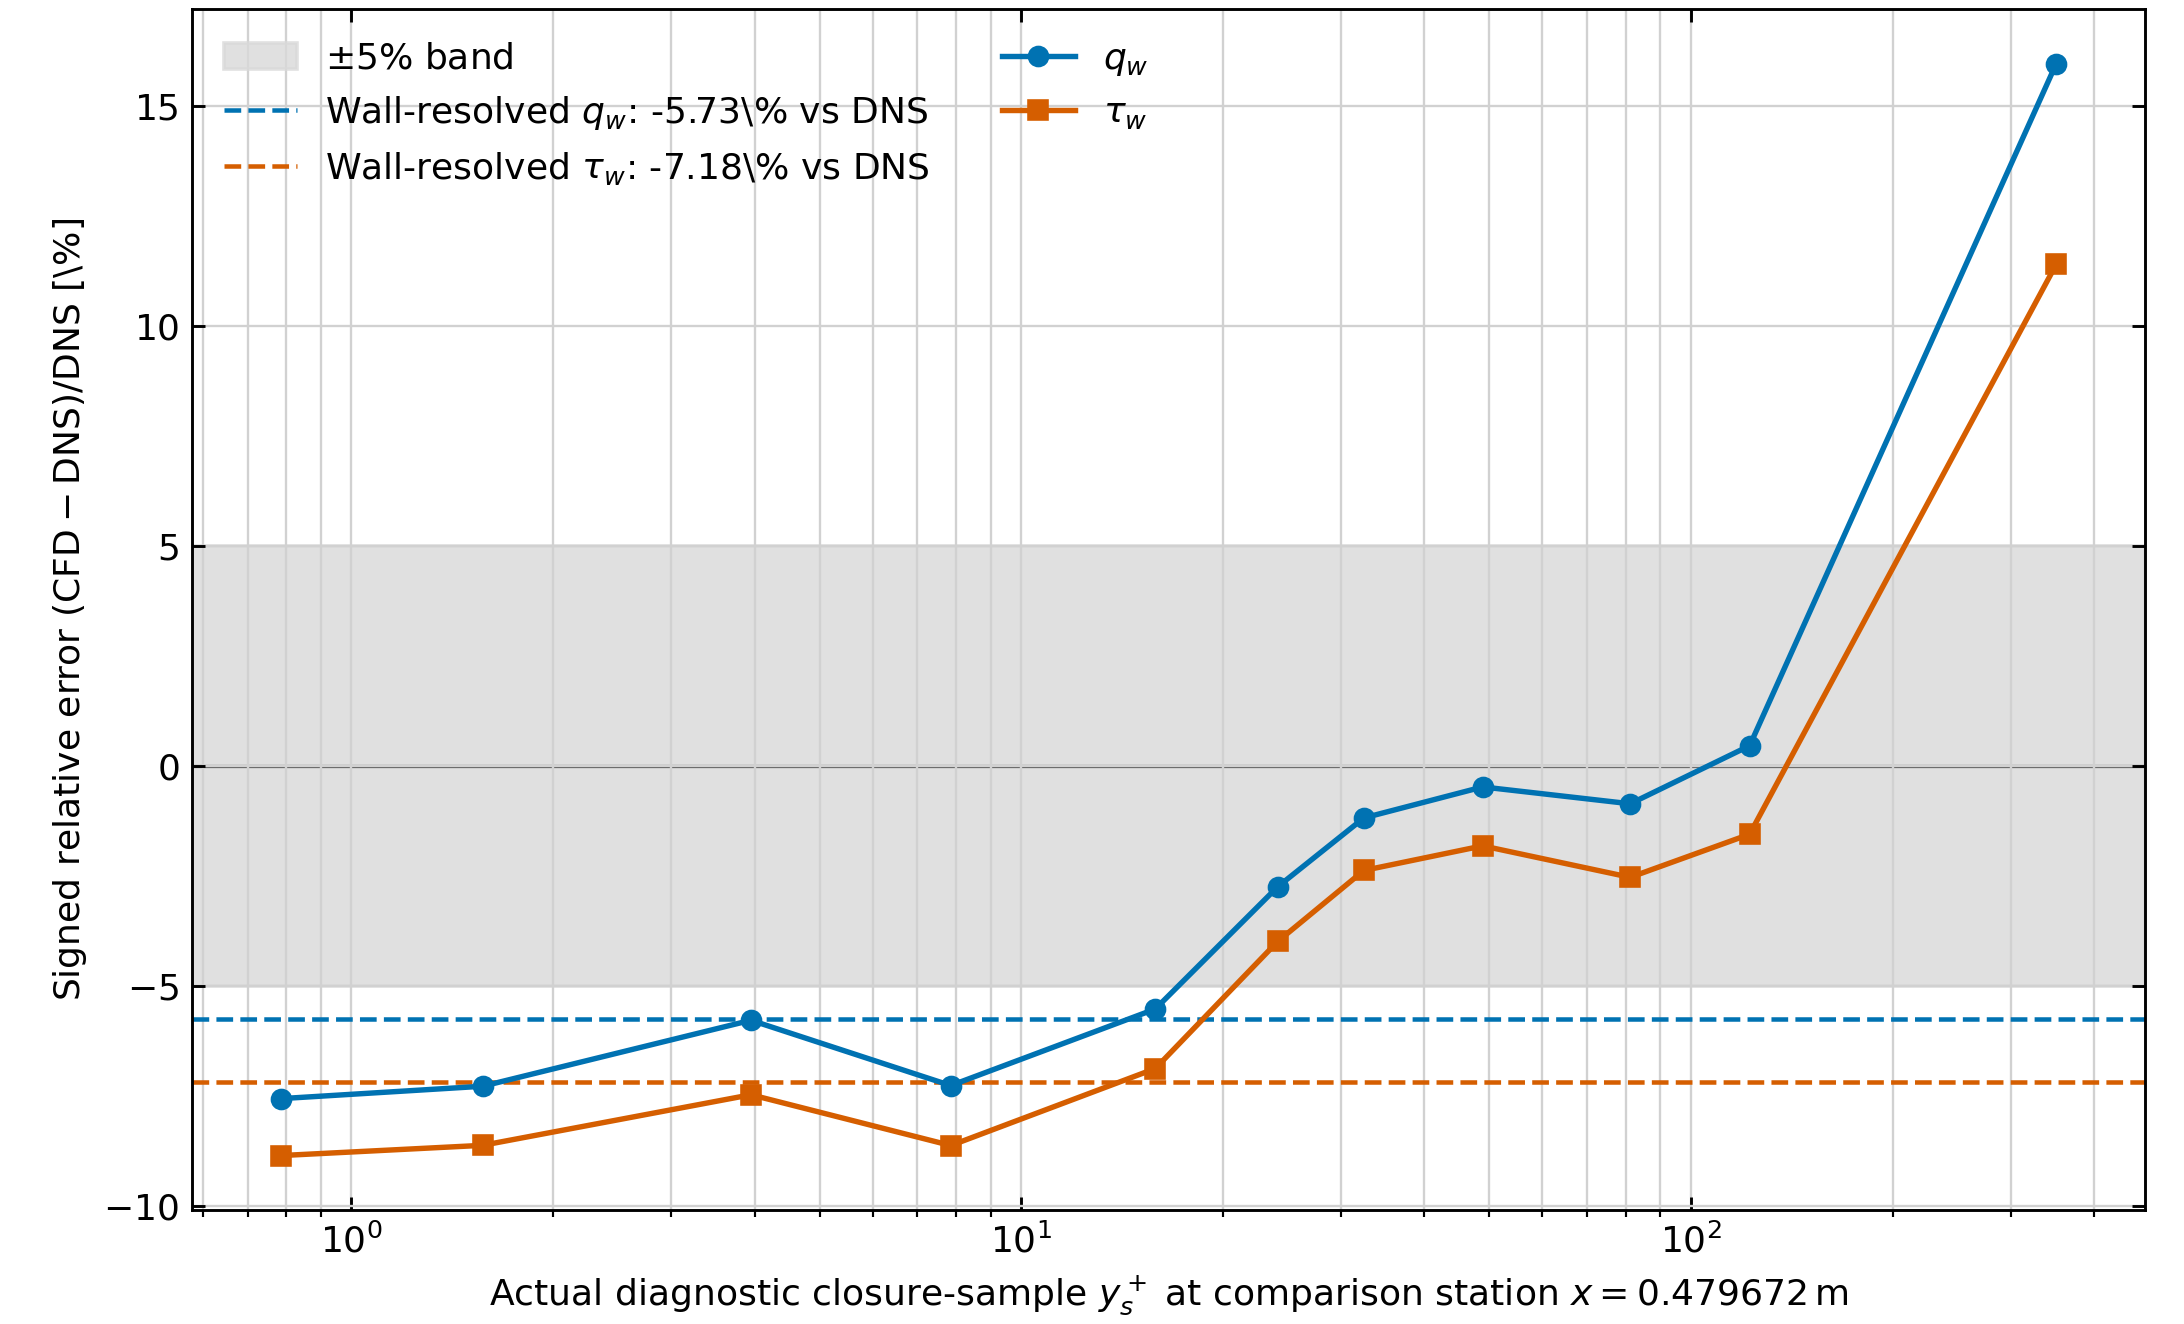
\includegraphics[width=\linewidth,height=.40\textheight,keepaspectratio]{07_Error_Isolation_Results/Figures/WallFunctions/04_3pctMesh_Li_LowHM3.png}
    % Figure provenance (WSL; absolute paths):
    %   Figure: /home/mgnadlinger/WF_validation/LowH_M3/validation/outputs/plots/opt_mesh/griffin_3pct_mincells_sa_dns_station_relative_error.png
    %   Python scripts:
    %     /home/mgnadlinger/WF_validation/LowH_M3/validation/scripts/plot_opt_mesh_wall_flux_sweeps.py
    %     /home/mgnadlinger/WF_validation/LowH_M3/validation/scripts/plot_wall_flux_sweeps.py
    %   Data / simulation roots (high-level):
    %     /home/mgnadlinger/WF_validation/LowH_M3/opt_meshes/Griffin_3pct_minCells_SA
    %     /home/mgnadlinger/WF_validation/LowH_M3/wall_resolved/SA/LowH_M3
    %     /home/mgnadlinger/WF_validation/LowH_M3/Digitizations
    % End figure provenance.
    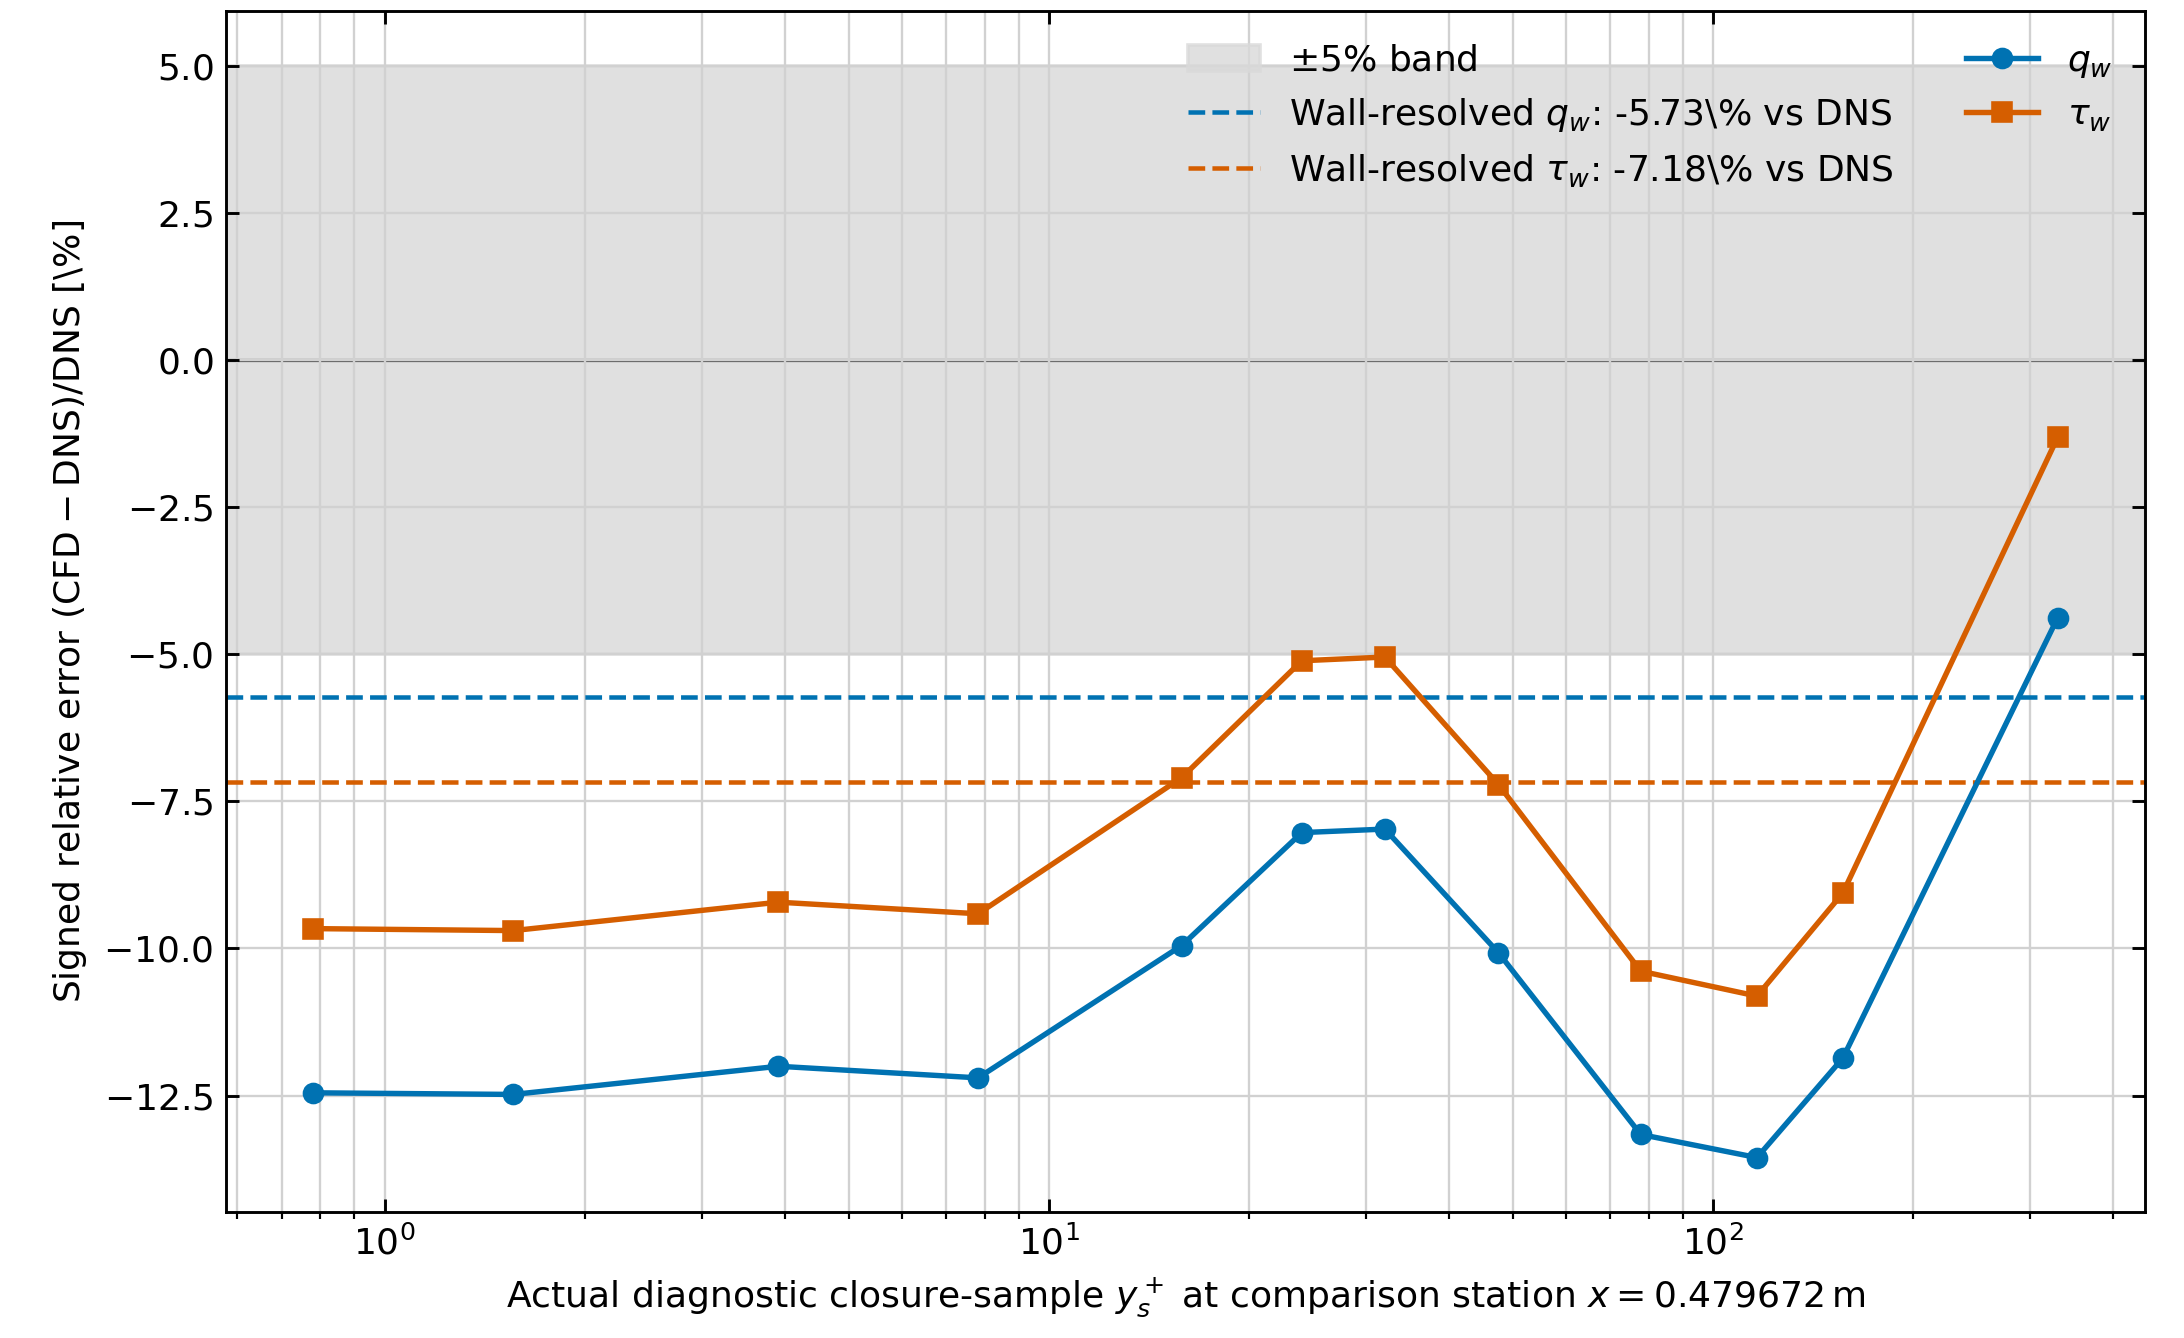
\includegraphics[width=\linewidth,height=.40\textheight,keepaspectratio]{07_Error_Isolation_Results/Figures/WallFunctions/04_3pctMesh_Griffin_LowHM3.png}
    \caption{Wall-function CFD on boundary layer-informed meshes designed with the $3\%$ cubic-reference component criterion. LowH\_M3 results are shown for Li (top) and Griffin (bottom). The abscissa is the actual diagnostic sampling location $y_s^+$ for the wall-function, not the first cell height. Dashed lines denote the wall-resolved baseline; shading marks $\pm5\%$ relative to DNS.}
    \label{fig:WF:3pct-bl-informed-mesh-CFD-results}
\end{figure}q

\begin{figure}[H]
    \ContinuedFloat
    \centering
    % Figure provenance (WSL; absolute paths):
    %   Figure: /home/mgnadlinger/Xue_et_al/flat_plate/M6Tw025/validation/outputs/plots/opt_mesh/li_3pct_sa_dns_station_relative_error.png
    %   Python scripts:
    %     /home/mgnadlinger/Xue_et_al/flat_plate/M6Tw025/validation/scripts/plot_opt_mesh_wall_flux_sweeps.py
    %     /home/mgnadlinger/Xue_et_al/flat_plate/M6Tw025/validation/scripts/plot_wall_flux_sweeps.py
    %   Data / simulation roots (high-level):
    %     /home/mgnadlinger/Xue_et_al/flat_plate/M6Tw025/opt_mesh/Li_3pct_SA
    %     /home/mgnadlinger/Xue_et_al/flat_plate/M6Tw025/Li_SA/SA_Prt0p9_baseline
    %     /home/mgnadlinger/Xue_et_al/flat_plate/M6Tw025/Digitizations
    %     /home/mgnadlinger/Xue_et_al/flat_plate/M6Tw025/opt_mesh/reference/sources
    % End figure provenance.
    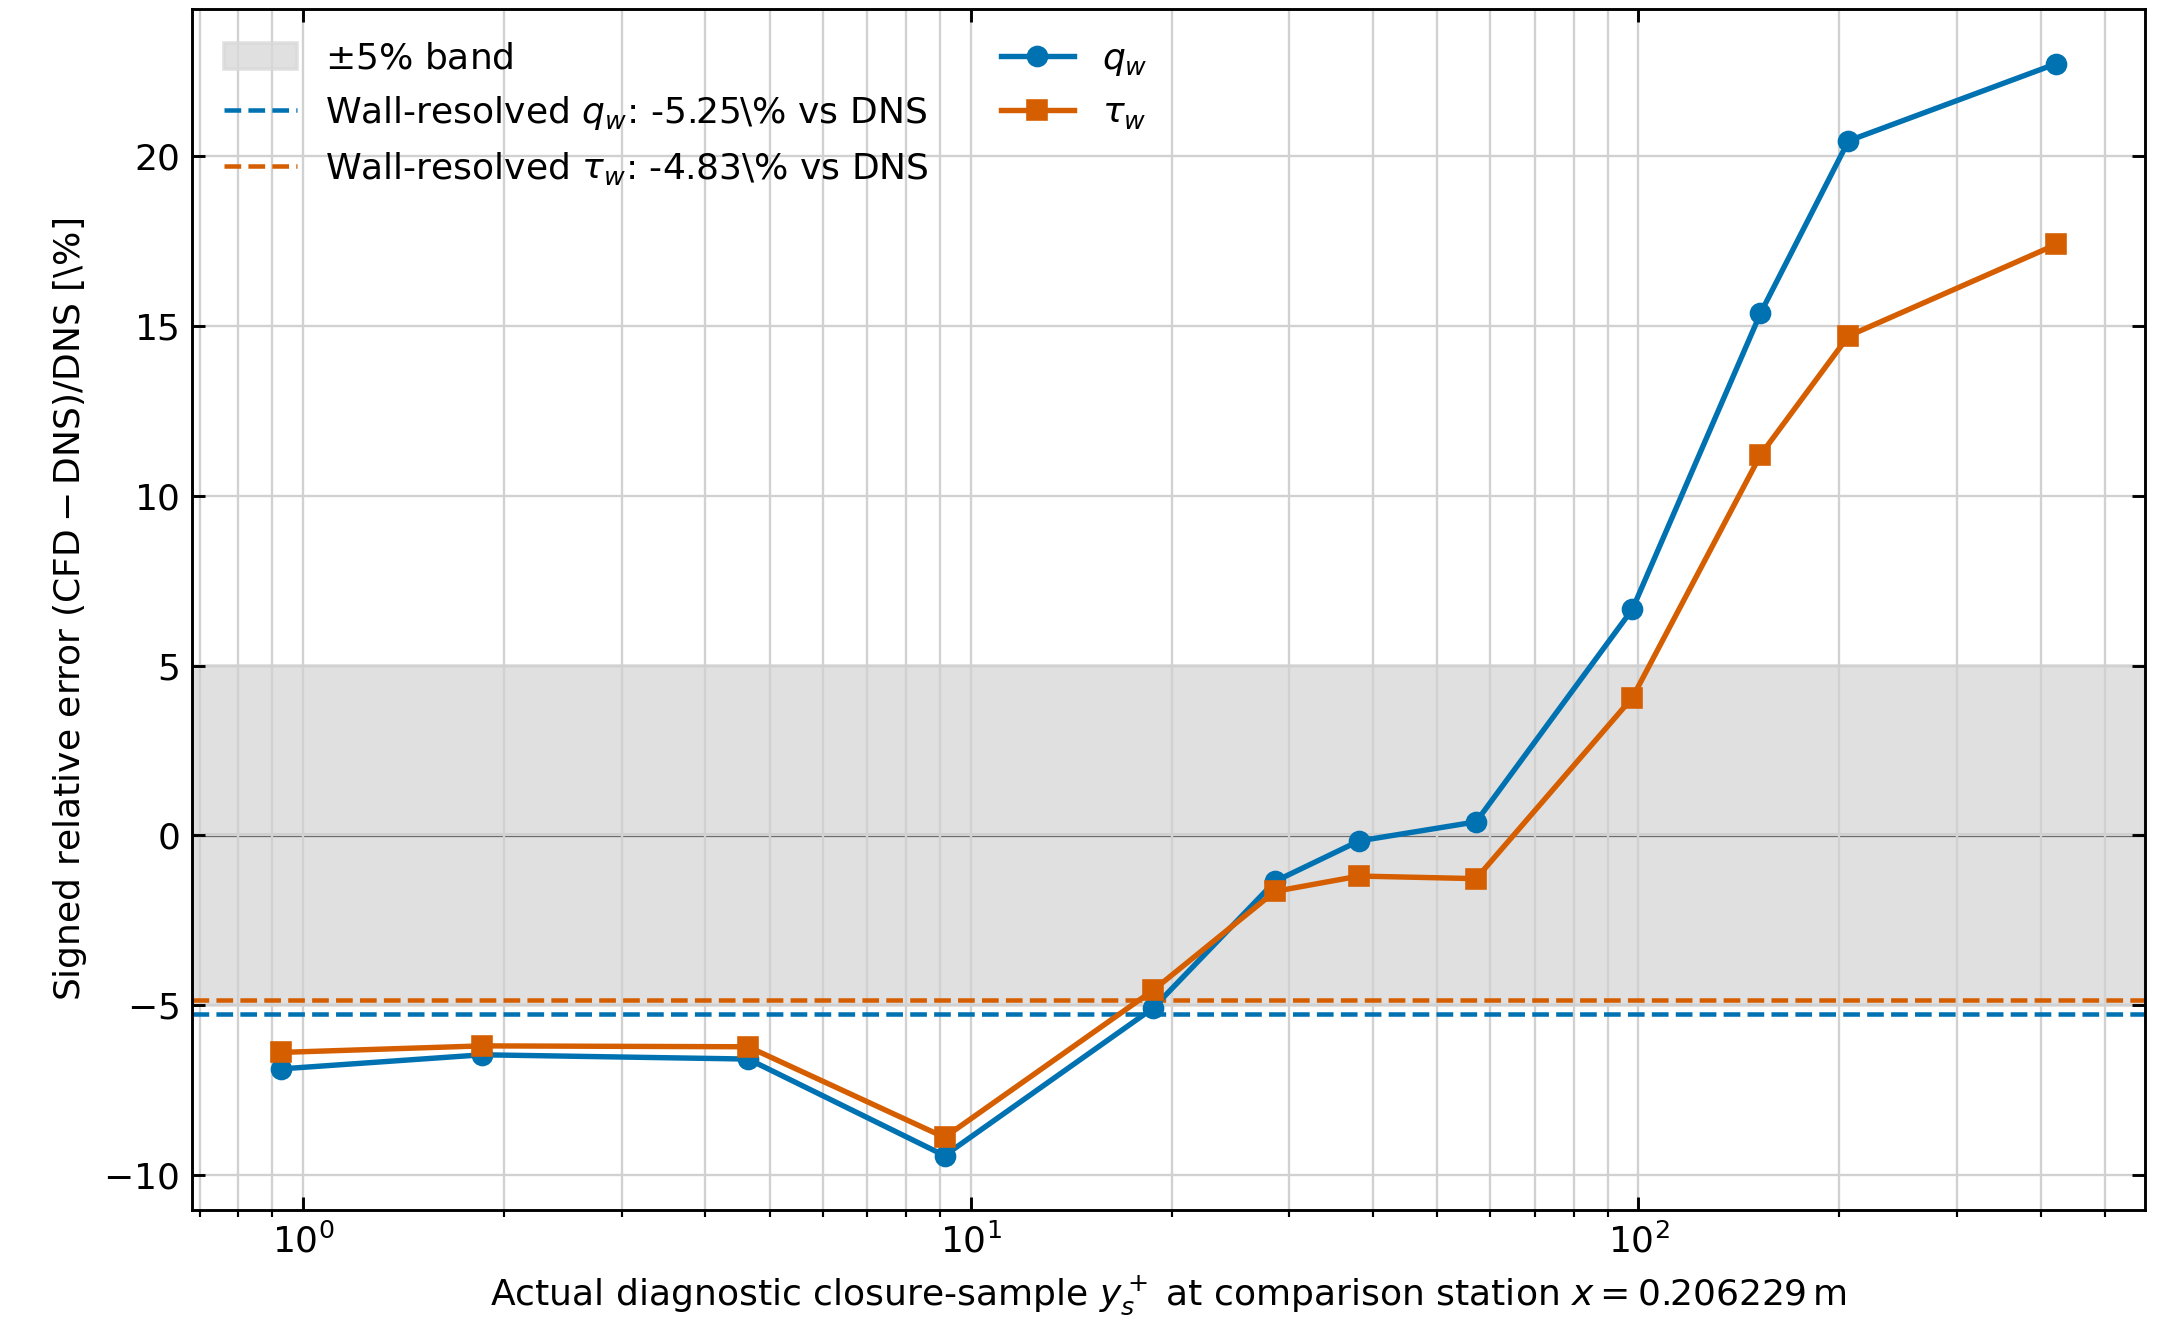
\includegraphics[width=\linewidth,height=.40\textheight,keepaspectratio]{07_Error_Isolation_Results/Figures/WallFunctions/04_3pctMesh_Li_M6Tw025.png}
    % Figure provenance (WSL; absolute paths):
    %   Figure: /home/mgnadlinger/Xue_et_al/flat_plate/M6Tw025/validation/outputs/plots/opt_mesh/griffin_3pct_sa_dns_station_relative_error.png
    %   Python scripts:
    %     /home/mgnadlinger/Xue_et_al/flat_plate/M6Tw025/validation/scripts/plot_opt_mesh_wall_flux_sweeps.py
    %     /home/mgnadlinger/Xue_et_al/flat_plate/M6Tw025/validation/scripts/plot_wall_flux_sweeps.py
    %   Data / simulation roots (high-level):
    %     /home/mgnadlinger/Xue_et_al/flat_plate/M6Tw025/opt_mesh/Griffin_3pct_SA
    %     /home/mgnadlinger/Xue_et_al/flat_plate/M6Tw025/Li_SA/SA_Prt0p9_baseline
    %     /home/mgnadlinger/Xue_et_al/flat_plate/M6Tw025/Digitizations
    %     /home/mgnadlinger/Xue_et_al/flat_plate/M6Tw025/opt_mesh/reference/sources
    % End figure provenance.
    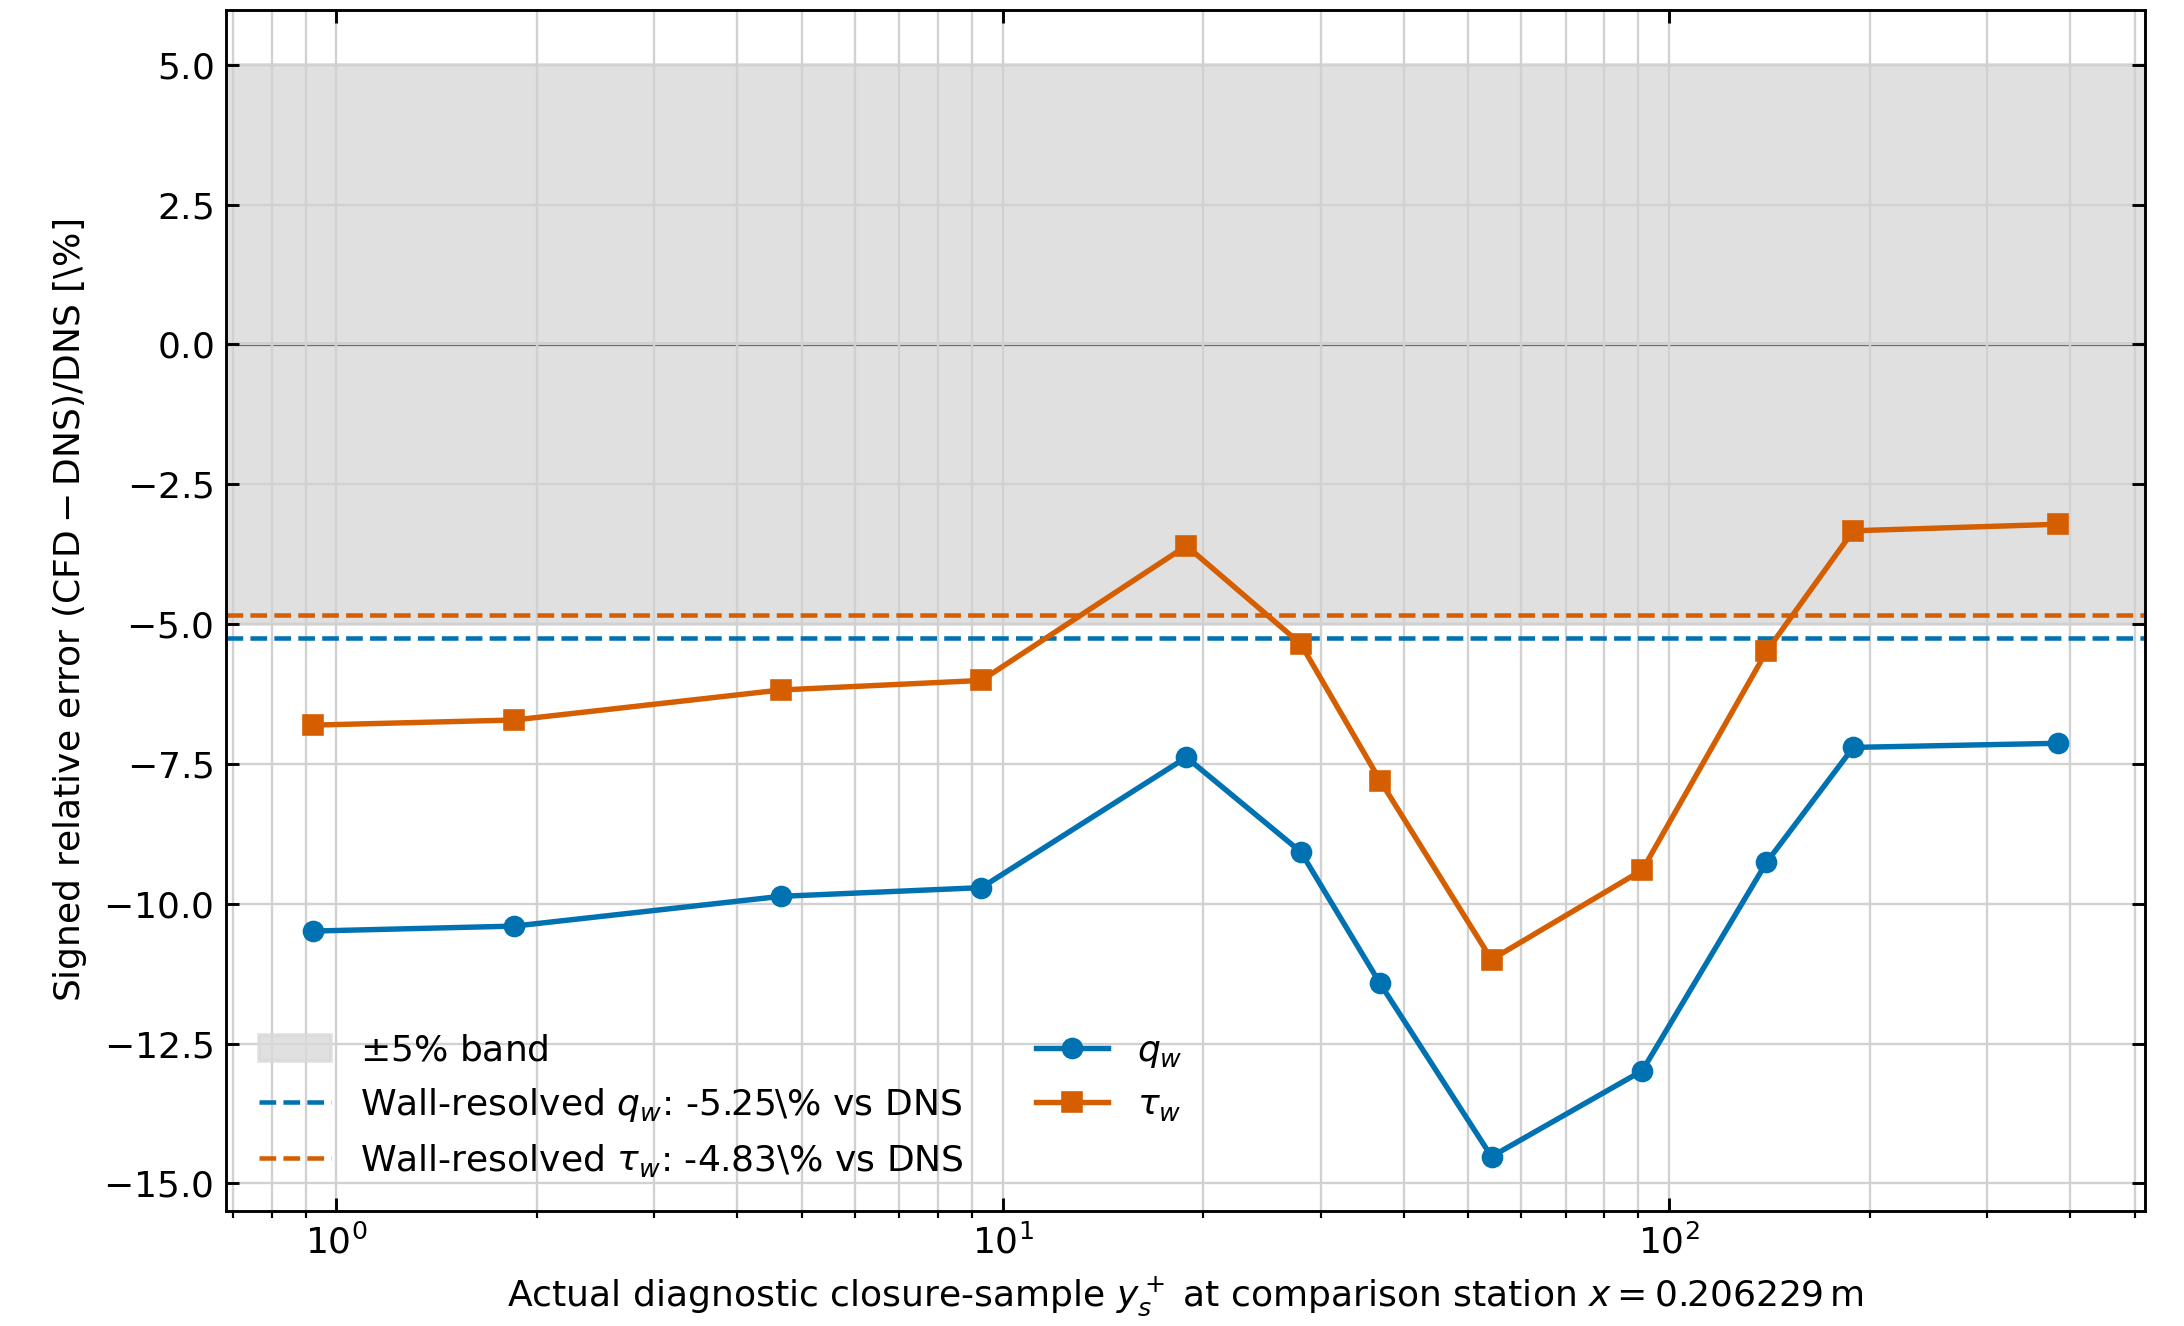
\includegraphics[width=\linewidth,height=.40\textheight,keepaspectratio]{07_Error_Isolation_Results/Figures/WallFunctions/04_3pctMesh_Griffin_M6Tw025.png}
    \caption[]{M6Tw025 results for Li (top) and Griffin (bottom), with SA and DNS normalization at $x=0.206229\,\mathrm{m}$. The mesh criterion and sampling-height definition are the same as in the preceding panels.}
\end{figure}

\subsection{Conditional a-priori estimation of the mesh requirement}
\label{subsec:comparative:zpg:apriori-mesh}

The above analysis and the novel proposed boundary layer informed meshing criterion, has one practical shortcoming: it requires knowledge of the resolved boundary layer profile. For an engineering approach, it is desirable to have a mesh design tool that does not require the resolved profile, but can still provide a-priori guidance on the required mesh spacing. The closures of the analytical Li et al. wall-function \cite{li2025WF} have this knowledge about hypersonic boundary layer backed in by design. Given wall shear and heat-flux, wall thermodynamic and transport properties, and an edge state, the wall-function closures can reconstruct the underlying profiles from which then the same finite-stencil limits can be evaluated. In the constant-$c_p$ form used here, the enthalpy relation supplies temperature from velocity, and the velocity law supplies the wall-normal coordinate. Under the additional constant-total-shear assumption, effective viscosity follows from $\mu_{\mathrm{eff}}=\tau_w/(\partial U/\partial y)$. Prescribed molecular and turbulent Prandtl numbers then give an effective conductivity estimate.
\par\medskip

Figure~\ref{fig:WF:a-priori-M6Tw025-10pct-envelope-combined} compares this estimate with the M6Tw025 profile-based envelope at a $10\%$ error tolerance. The reconstruction uses scalar DNS metadata for the wall loads and edge/wall states, without using the resolved profile values. It is therefore an assessment conditional on known loads, rather than an independent prediction of those loads. The broad inner-layer spacing trend is recovered, but the most restrictive minimum is shifted because the Li reconstruction places the temperature maximum closer to the wall. Near that maximum, even a modest position error can produce a large difference in the relative-gradient criterion. Differences toward the boundary layer edge also reflect the limited outer-layer representation of the reconstructed inner law.

\begin{figure}[H]
    \centering
    % Figure provenance (WSL; absolute paths):
    %   Figure: /home/mgnadlinger/Xue_et_al/flat_plate/M6Tw025/opt_mesh/li_apriori/M6Tw025_Li_combined_comparison_10pct_only.png
    %   Python scripts:
    %     /home/mgnadlinger/Xue_et_al/flat_plate/M6Tw025/opt_mesh/li_apriori/plot_10pct_combined_only.py
    %     /home/mgnadlinger/Xue_et_al/flat_plate/M6Tw025/opt_mesh/li_apriori/li_apriori_spacing.py
    %   Data / simulation roots (high-level):
    %     /home/mgnadlinger/Xue_et_al/flat_plate/M6Tw025/opt_mesh/li_apriori
    %     /home/mgnadlinger/Xue_et_al/flat_plate/M6Tw025/opt_mesh/spacing_limits
    %     /home/mgnadlinger/Xue_et_al/flat_plate/M6Tw025/opt_mesh/reference
    %     /home/mgnadlinger/Xue_et_al/flat_plate/M6Tw025/Digitizations
    %     /home/mgnadlinger/Xue_et_al/flat_plate/M6Tw025/Li_SA/SA_Prt0p9_baseline
    %   Note: Thesis image is cropped from the source export at native resolution, without resizing.
    %     Crop box in source pixels (left, top, right, bottom): (0, 274, 2250, 2200);
    %     resulting size: 2250 x 1926 pixels. Original plot proportions are preserved.
    %   Note: li_apriori_spacing.py generates the prediction from DNS scalar header inputs; the frozen DNS/SA
    %     reference supplies the comparison envelope.
    % End figure provenance.
    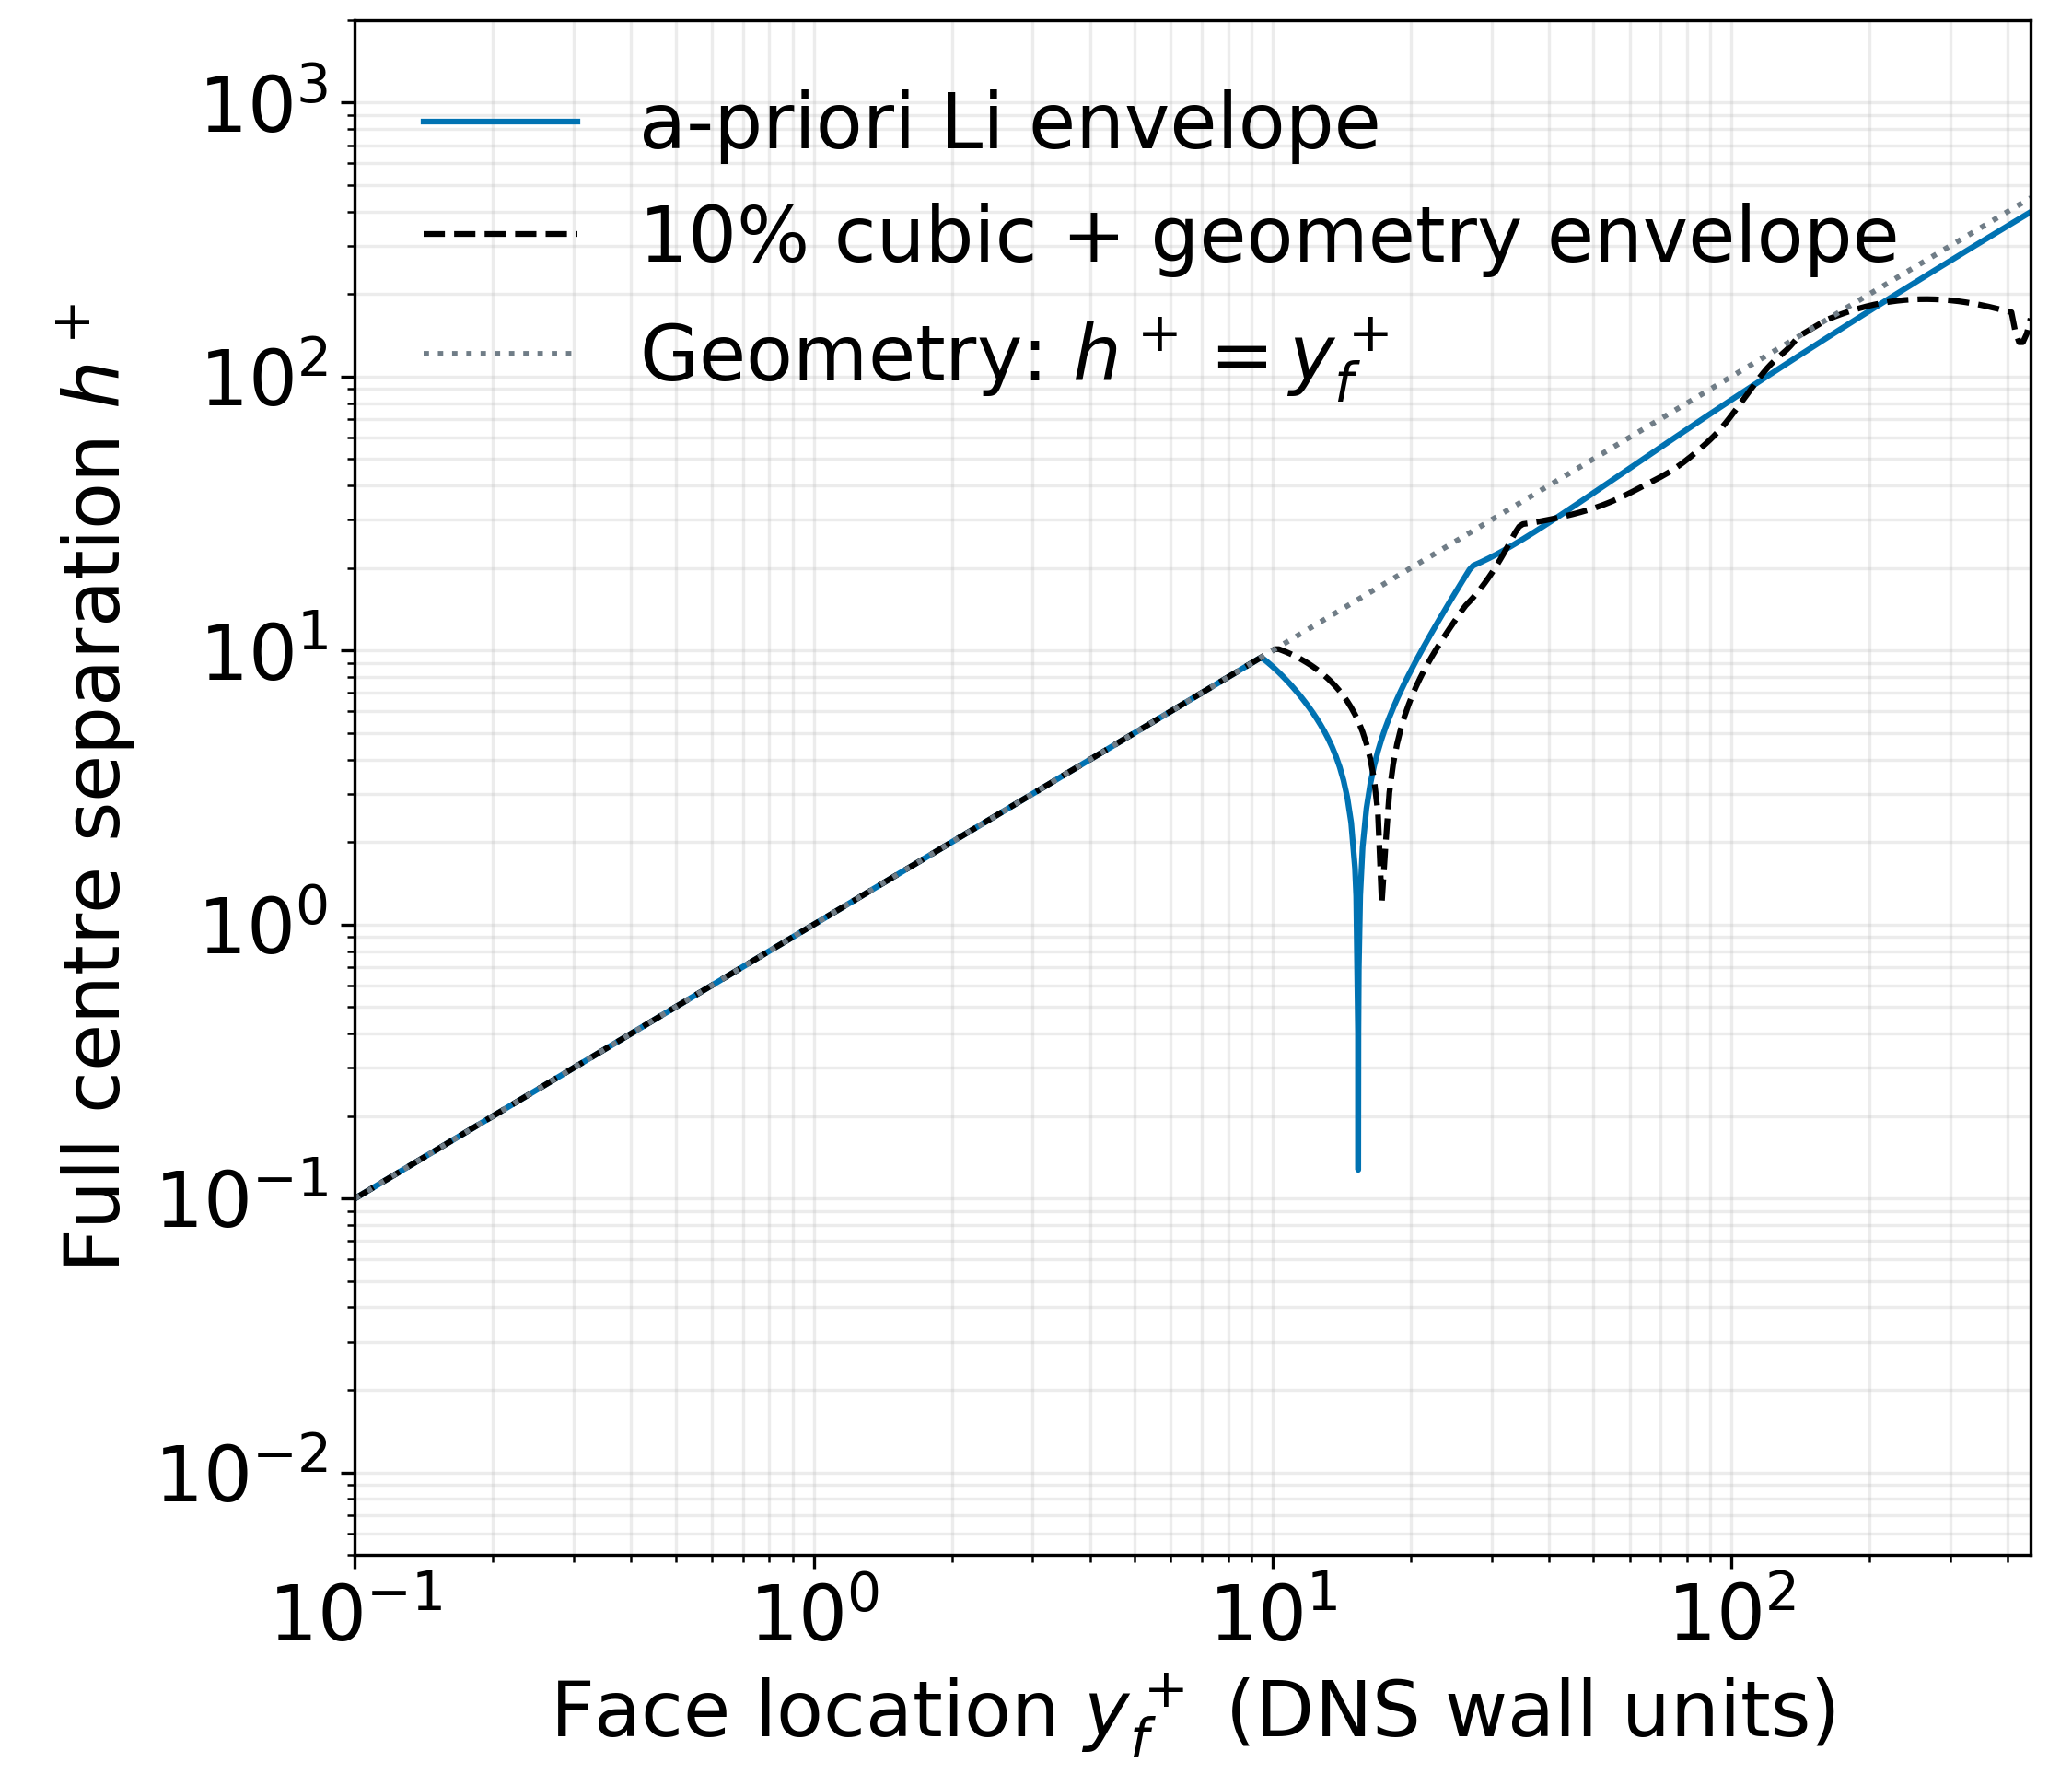
\includegraphics[width=.7\linewidth,height=.54\textheight,keepaspectratio]{07_Error_Isolation_Results/Figures/WallFunctions/apriori_M6_mesh.png}
    \caption{Conditional a-priori estimate of the M6Tw025 $10\%$ spacing envelope from the Li relations (blue), compared with the profile-based cubic-reference envelope (black dashed). The reconstruction uses scalar wall loads, wall/edge states and transport properties, without the resolved boundary layer profile. The geometric cap is dotted. The displaced restrictive minimum near the temperature maximum limits the estimate's use as an accuracy guarantee.}
    \label{fig:WF:a-priori-M6Tw025-10pct-envelope-combined}
\end{figure}

The estimate can consequently guide an initial mesh design or identify a likely region of refinement. Practical use also requires suitable estimates of wall loads and edge quantities. For the present zero-pressure-gradient flat-plates these inputs are comparatively well defined. The boundary layer edge states can be approximated to the freestream conditions, and for the wall heat-flux and shear stress on zero-pressure-gradient flat-plates analytical approximations like the theory of van Driest are available. Their approximation and the validity of the equilibrium assumptions are however more challenging for complex flows.

\subsection{Recovery of the wall-resolved baseline with fitted closures}
\label{subsec:comparative:zpg:fitted-closure}
 
The remaining question, to close the error isolation loop, is whether the wall-function formulation can recover the wall-resolved solution when both its closure relations and spatial discretization errors are removed. LowH\_M3 provides a suitable diagnostic case because its wall-resolved SA thermal-profile shape agrees comparatively well with DNS, thus also eliviating the implications of the turbulence model. The Li formulation is retained, but its velocity and enthalpy relations are fitted to the wall-resolved SA field of the LowH\_M3 case.
\par\medskip

Lookup tables for the wall function's momentum and enthalpy closures are constructed from the wall-resolved SA boundary layer profiles, using the reference wall shear stress, wall heat-flux and local boundary layer edge velocity and temperature. The tables store the fitted velocity relation and a correction to the Li enthalpy relation. During CFD, the fitted closure relations determine wall shear stress and wall heat-flux from the wall-function sample station's velocity and temperature, while the fitted velocity-law derivative supplies the near-wall constraint on the SA variable $\tilde{\nu}$ (Section~\ref{subsec:wall-functions:gao-li:turbulence-coupling}). The construction therefore requires reference profiles at multiple streamwise stations and the singular published DNS profiles are insufficient.
\par\medskip

Figure~\ref{fig:WF:a-priori-Li-fitted-LowHM3} first checks the fitted closure relations using the same a-priori approach as in Section~\ref{subsec:erriso:apriori-solver}. The recovered heat-flux and shear stress differ from the wall-resolved targets by order $10^{-7}\%$. This near-exact recovery verifies the reference-conditioned inverse construction at the sampled states.

\begin{figure}[H]
    \centering
    % Figure provenance (WSL; absolute paths):
    %   Figure: /home/mgnadlinger/OpenFOAM/mgnadlinger-v2412/src/LiWallFunctions/tests/ReverseSolver/LowH_M3_Duan_Li_fitted/wall_flux_errors_vs_yplus.png
    %   Python scripts:
    %     /home/mgnadlinger/OpenFOAM/mgnadlinger-v2412/src/LiWallFunctions/tests/ReverseSolver/analyze_li_fitted_wall_function_profile_Duan.py
    %     /home/mgnadlinger/OpenFOAM/mgnadlinger-v2412/src/LiWallFunctions/tests/ReverseSolver/build_lowh_m3_fitted_model.py
    %   Data / simulation roots (high-level):
    %     /home/mgnadlinger/OpenFOAM/mgnadlinger-v2412/src/LiWallFunctions/tests/ReverseSolver/LowH_M3_Duan
    %     /home/mgnadlinger/OpenFOAM/mgnadlinger-v2412/src/LiWallFunctions/tests/ReverseSolver/LowH_M3_Duan_Li/constant/LiLowHM3Fit
    %     /home/mgnadlinger/OpenFOAM/mgnadlinger-v2412/src/LiWallFunctions/tests/ReverseSolver/LowH_M3_Duan_Li_fitted
    %     /home/mgnadlinger/Duan_DNS_ZPGFP/Martin_Duan_Part4/SA_Prt0p9/LowH_M3
    %     /home/mgnadlinger/WF_validation/LowH_M3/wall_resolved/SA/LowH_M3
    %     /home/mgnadlinger/WF_validation/LowH_M3/Li_SA
    %   Note: Closure input is the wall-resolved SA profile at time 20000.
    %   Note: Thesis image is resized from the source export. The fitted model uses wall-resolved SA profiles
    %     and Li_SA mesh geometry.
    % End figure provenance.
    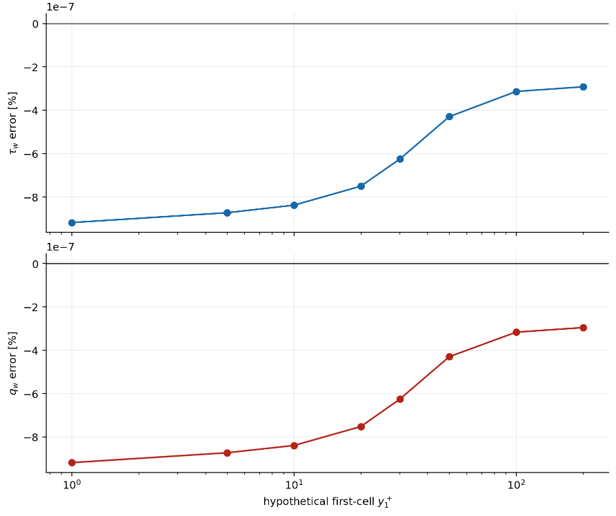
\includegraphics[width=\linewidth,height=.43\textheight,keepaspectratio]{07_Error_Isolation_Results/Figures/WallFunctions/a-priori-Li-fitted-LowHM3.png}
    \caption{A-priori inverse recovery using the fitted LowH\_M3 Li relations and samples from the wall-resolved SA reference. Recovered shear stress (top) and heat-flux (bottom) are compared with that same reference. Errors are of order $10^{-7}\%$, as indicated by the axis multipliers; this is consistency of the reference-conditioned inverse model, rather than independent DNS validation.}
    \label{fig:WF:a-priori-Li-fitted-LowHM3}
\end{figure}

The corresponding CFD result is shown in Figure~\ref{fig:WF:3pct-Li-fitted-LowHM3}. With the fitted relations and boundary layer-informed meshes, heat-flux and shear stress remain within approximately $\pm2\%$ of the wall-resolved values over the completed sampling sweep. Thus successfully isolating the errors caused by spatial discretization and wall-function closure theories. The last persistent error to the DNS reference, is the baseline error of the underlying wall-resolved RANS as discovered in the first Section~\ref{subsec:comparative:zpg:wr-wall-fluxes}. So it can be concluded, that with a boundary layer-informed mesh, improved closure relations and improved RANS turbulence modelling, the wall-function CFD could recover perfect wall heat-flux and shear stress.

\begin{figure}[H]
    \centering
    % Figure provenance (WSL; absolute paths):
    %   Figure: /home/mgnadlinger/WF_validation/LowH_M3/mesh_archives/20260908_before_leading_edge_refinement/Li_fitted_3pct_minCells_SA/results_analysis/wall_flux_sweep/plots/li_fitted_3pct_mincells_sa_dns_station_relative_error.png
    %   Python scripts:
    %     /home/mgnadlinger/WF_validation/LowH_M3/mesh_archives/20260908_before_leading_edge_refinement/Li_fitted_3pct_minCells_SA/results_analysis/run_wall_flux_sweep.py
    %     /home/mgnadlinger/WF_validation/LowH_M3/validation/scripts/plot_wall_flux_sweeps.py
    %   Data / simulation roots (high-level):
    %     /home/mgnadlinger/WF_validation/LowH_M3/mesh_archives/20260908_before_leading_edge_refinement/Li_fitted_3pct_minCells_SA
    %     /home/mgnadlinger/WF_validation/LowH_M3/wall_resolved/SA/LowH_M3
    %     /home/mgnadlinger/WF_validation/LowH_M3/Digitizations
    %   Note: Thesis image removes the 128-pixel title strip from the source export.
    %   Note: Displayed CFD results use the archived sweep from before the leading-edge mesh refinement on
    %     2026-09-08.
    %   Note: An identical full export is also retained at
    %     /home/mgnadlinger/WF_validation/LowH_M3/validation/outputs/plots/li_fitted_3pct_mincells_sa_dns_station_relative_error.png
    % End figure provenance.
    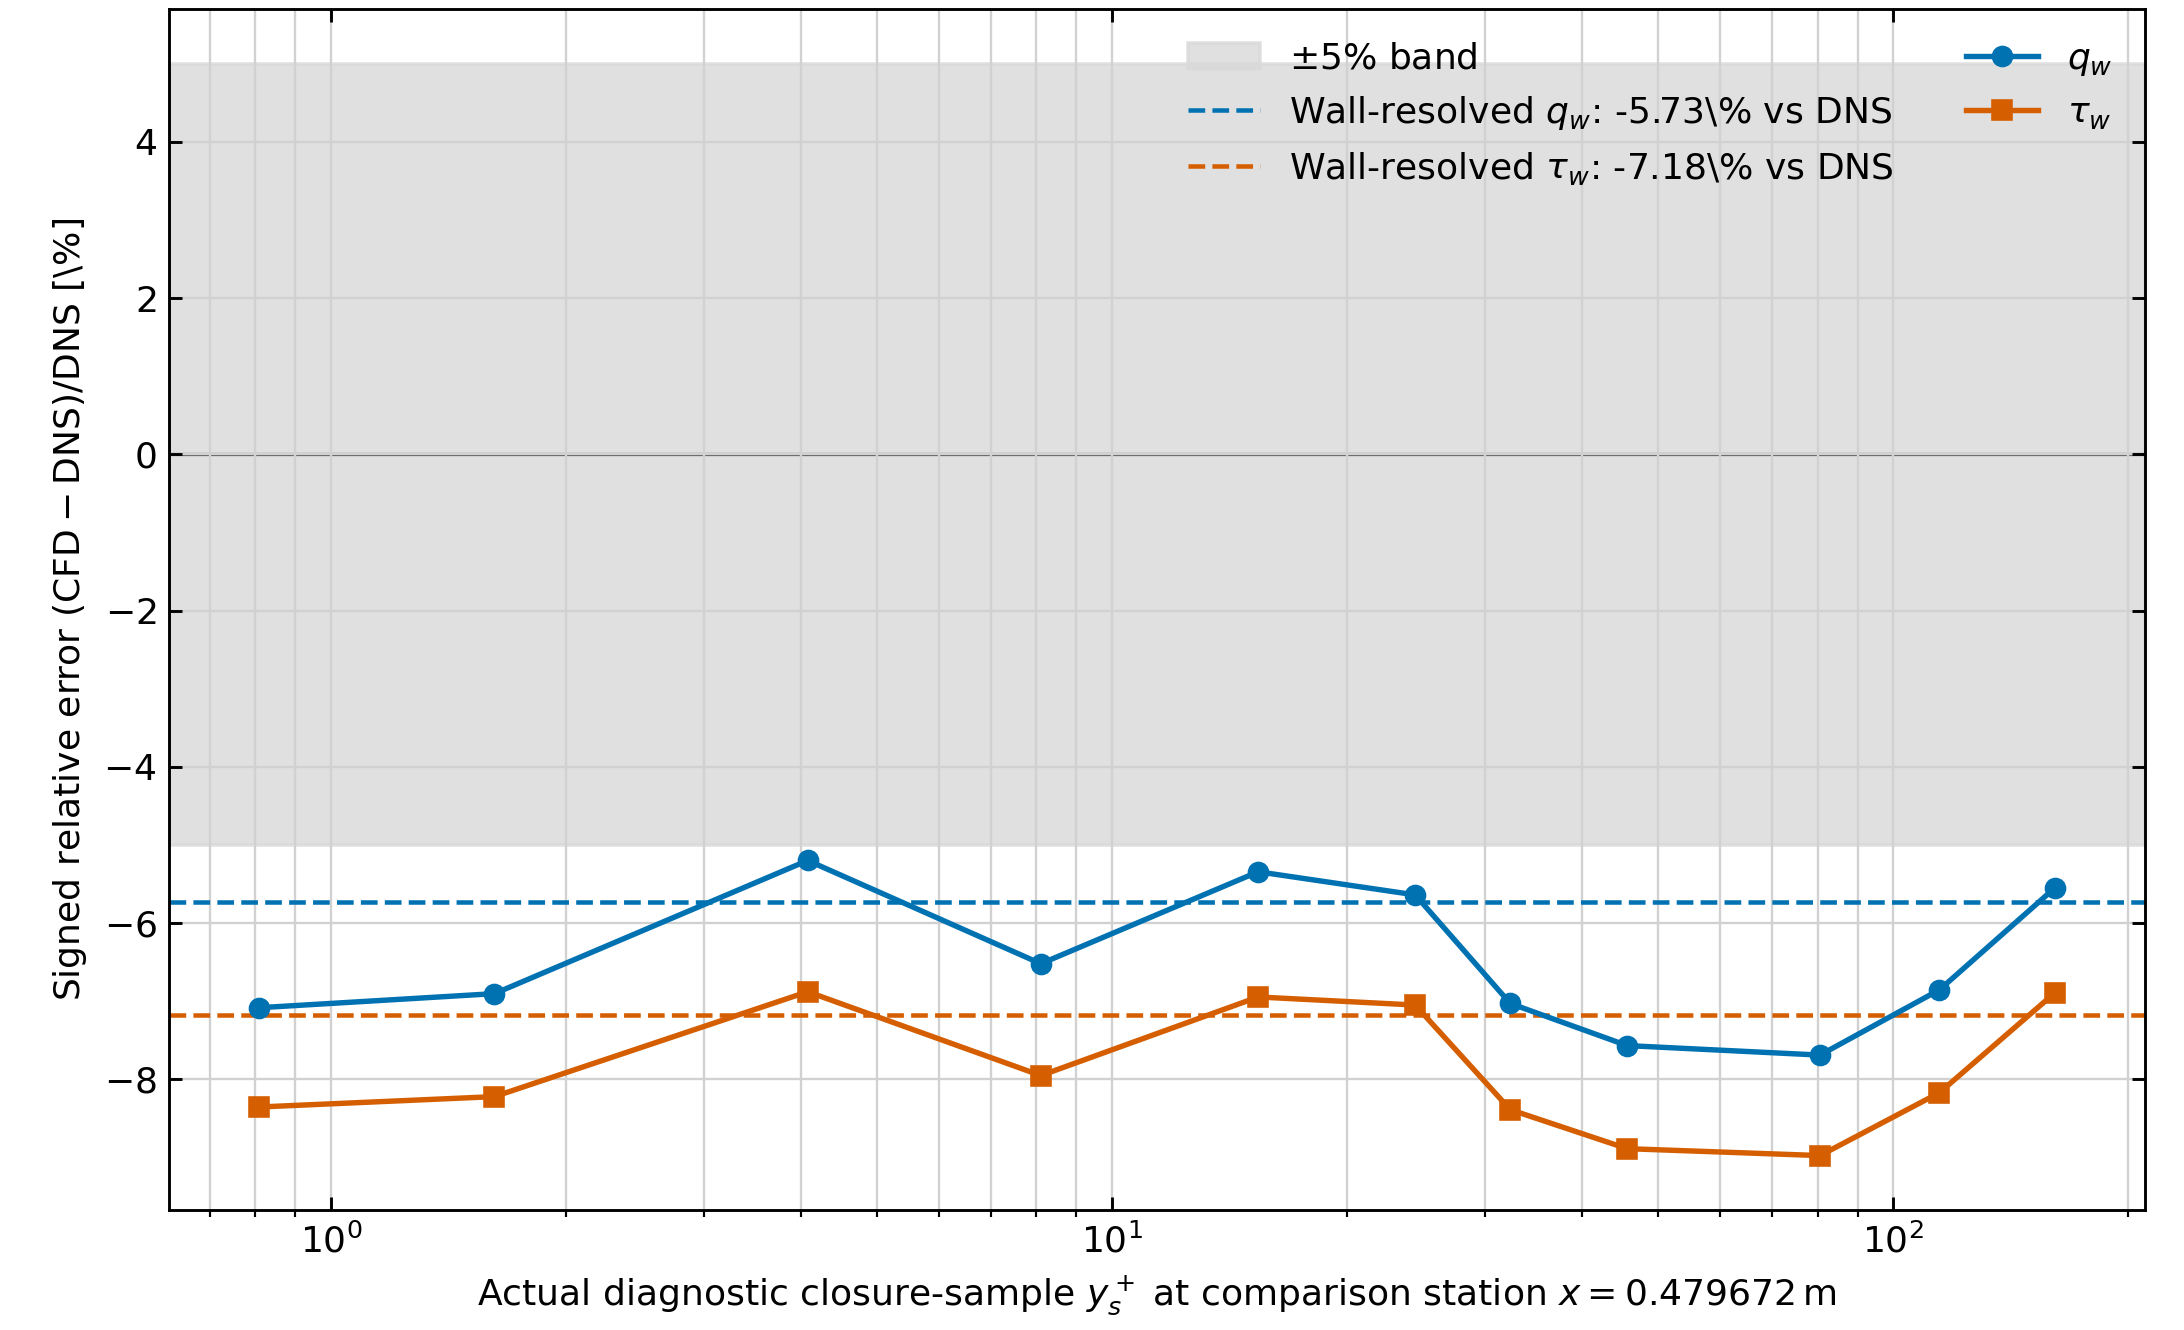
\includegraphics[width=\linewidth,height=.43\textheight,keepaspectratio]{07_Error_Isolation_Results/Figures/WallFunctions/04_3pctMesh_fitted_Li_LowHM3.png}
    \caption{LowH\_M3 CFD with fitted Li relations, SA and boundary layer-informed $3\%$ meshes. Signed errors in heat-flux and shear stress relative to DNS are plotted against the actual sampling location at $x=0.479672\,\mathrm{m}$. The curves remain close to the wall-resolved baseline (dashed), with deviations of approximately $\pm2\%$ when normalized by the corresponding wall-resolved quantities. Shading marks $\pm5\%$ relative to DNS.}
    \label{fig:WF:3pct-Li-fitted-LowHM3}
\end{figure}


\chapter{Conclusion and Outlook}
\label{chap:conclusion-outlook}

Through a successive isolation of errors from the turbulence model (ref. Section~\ref{sec:comparative:zpg:wall-resolved-baselines}), the underlying wall-function closure theory (ref. Section~\ref{sec:comparative:zpg:cross-comparison}) and the spatial discretization (ref. Section~\ref{subsec:comparative:zpg:yplus-sensitivity}), novel findings and strong assessments to the accuracy of the aerothermal prediction of RANS with and without wall-functions was formed.
\par\medskip

Figure~\ref{fig:conclusion:overview-of-isolation-of-errors} shows the isolation of errors, from conventional coarse wall function mesh (top), to novel boundary layer informed mesh (middle) to additional posterior fitting of the closure (bottom), which then all in all results in the wall function CFD to be within the wall resolved result to within +-2\% - i.e. all the errors have been fully isolated and investigated (within error cancellation still being a thing also). 
\begin{figure}[H]
    \centering
    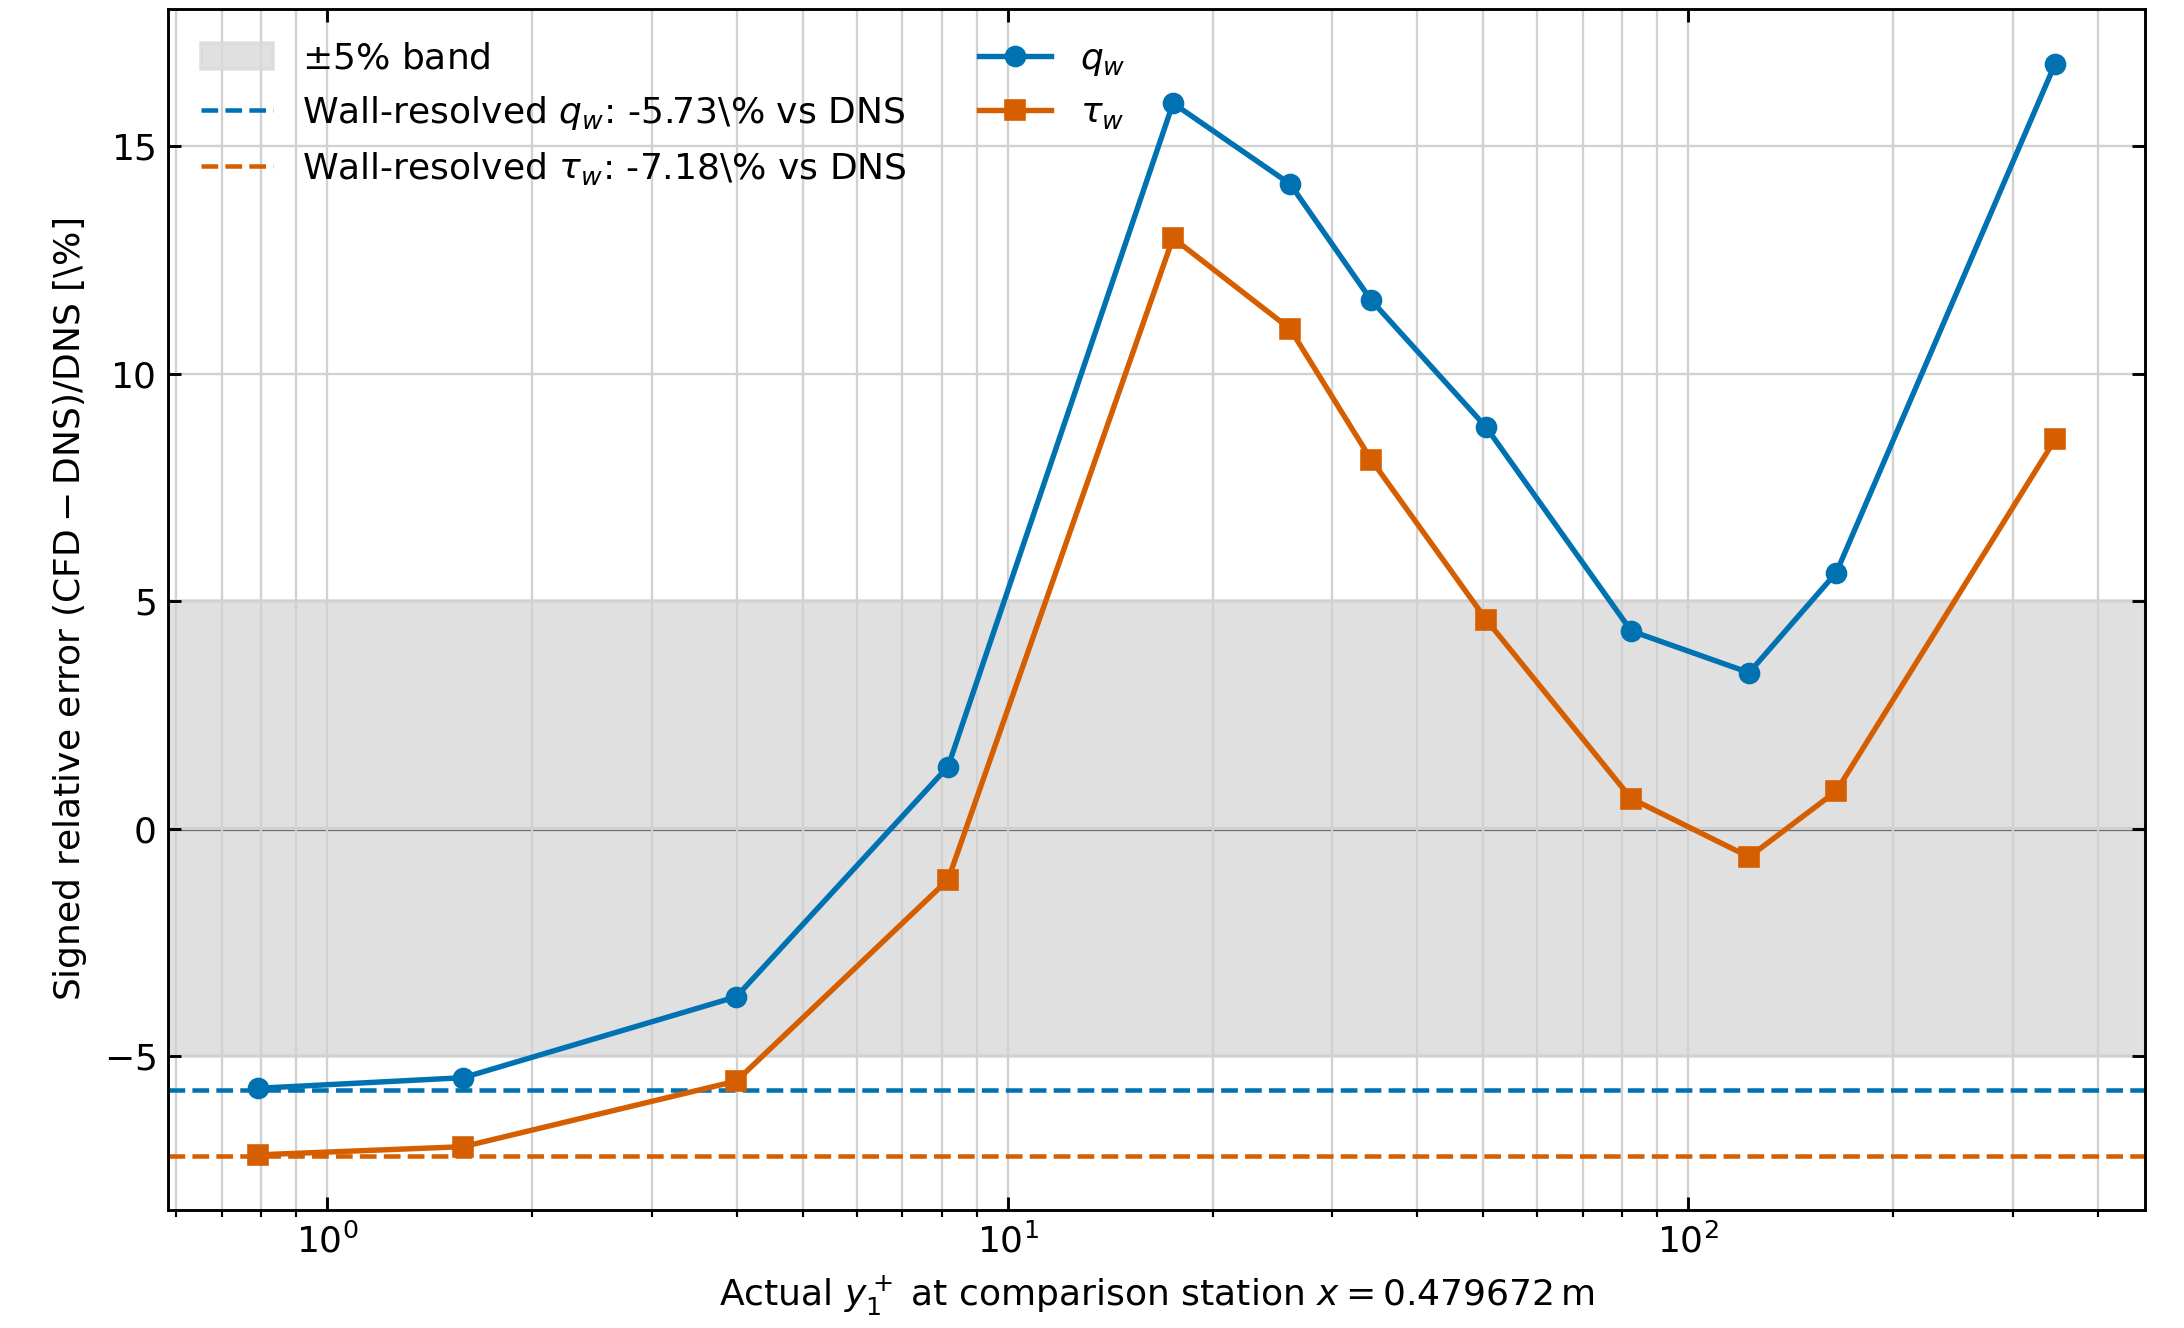
\includegraphics[width=\linewidth,height=.43\textheight,keepaspectratio]{07_Error_Isolation_Results/Figures/WallFunctions/04_ConvMesh_Li_LowHM3.png}
    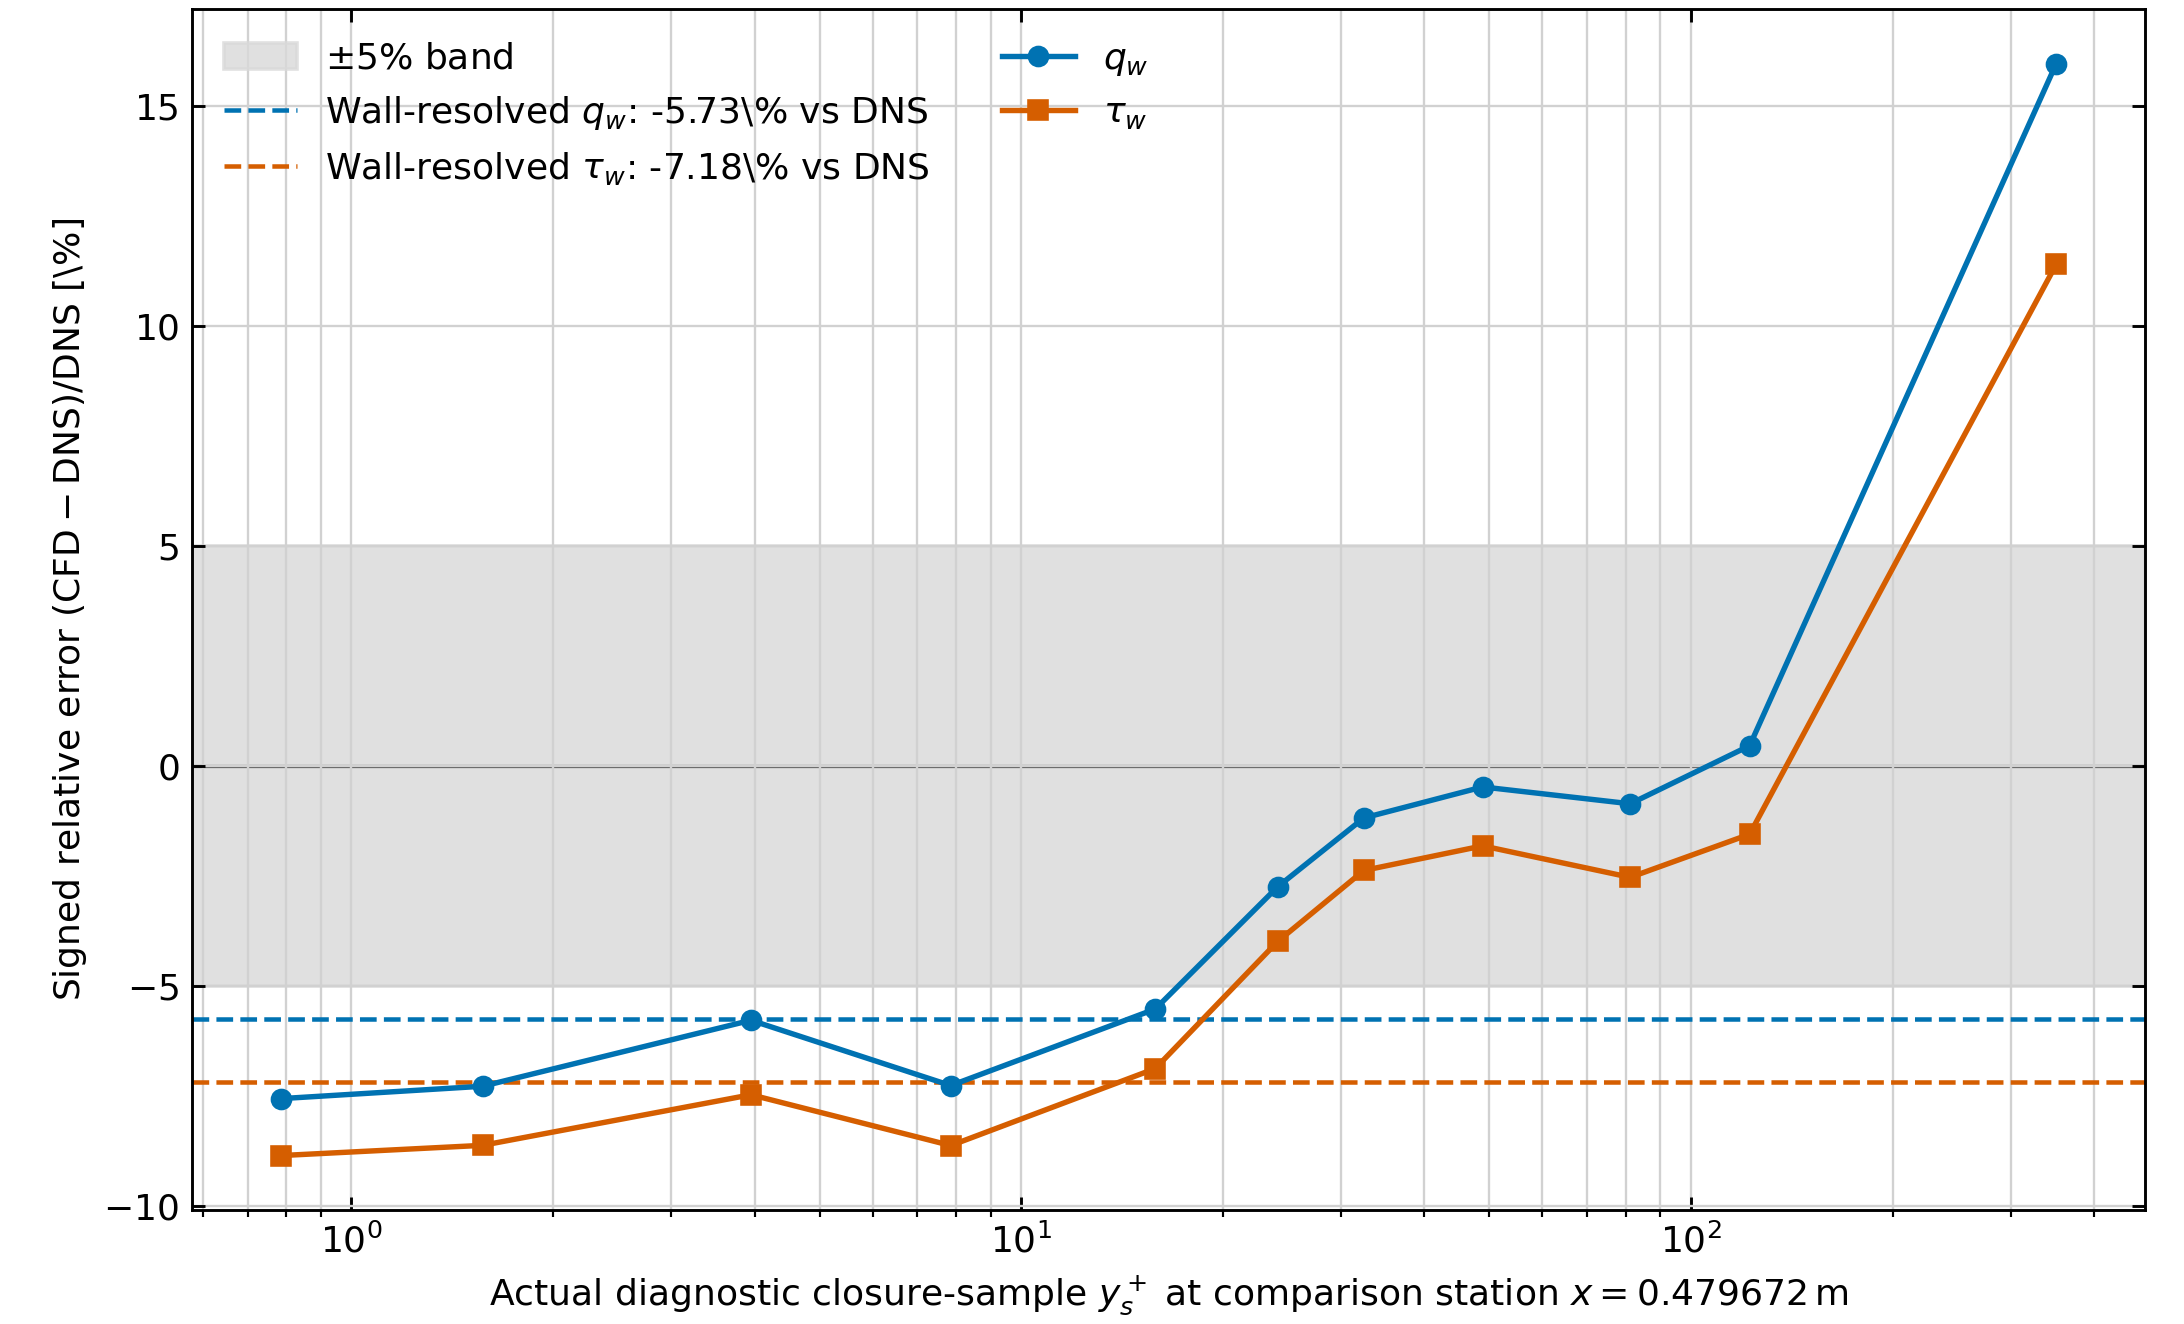
\includegraphics[width=\linewidth,height=.43\textheight,keepaspectratio]{07_Error_Isolation_Results/Figures/WallFunctions/04_3pctMesh_Li_LowHM3.png}
    \caption[Error-isolation sequence for LowH\_M3 with Li wall functions and SA.]{Error-isolation sequence for LowH\_M3 with Li wall functions and SA: conventional meshes (top), boundary layer-informed meshes (bottom), and fitted closures on informed meshes (continued). Signed wall heat-flux and shear-stress errors are relative to DNS; dashed lines show the wall-resolved SA baseline and shading marks the $\pm5\%$ DNS band. The abscissa is the first-cell location $y_1^+$ on conventional meshes and the sampling location $y_s^+$ on informed meshes.}
    \label{fig:conclusion:overview-of-isolation-of-errors}
\end{figure}
\begin{figure}[H]
    \ContinuedFloat
    \centering
    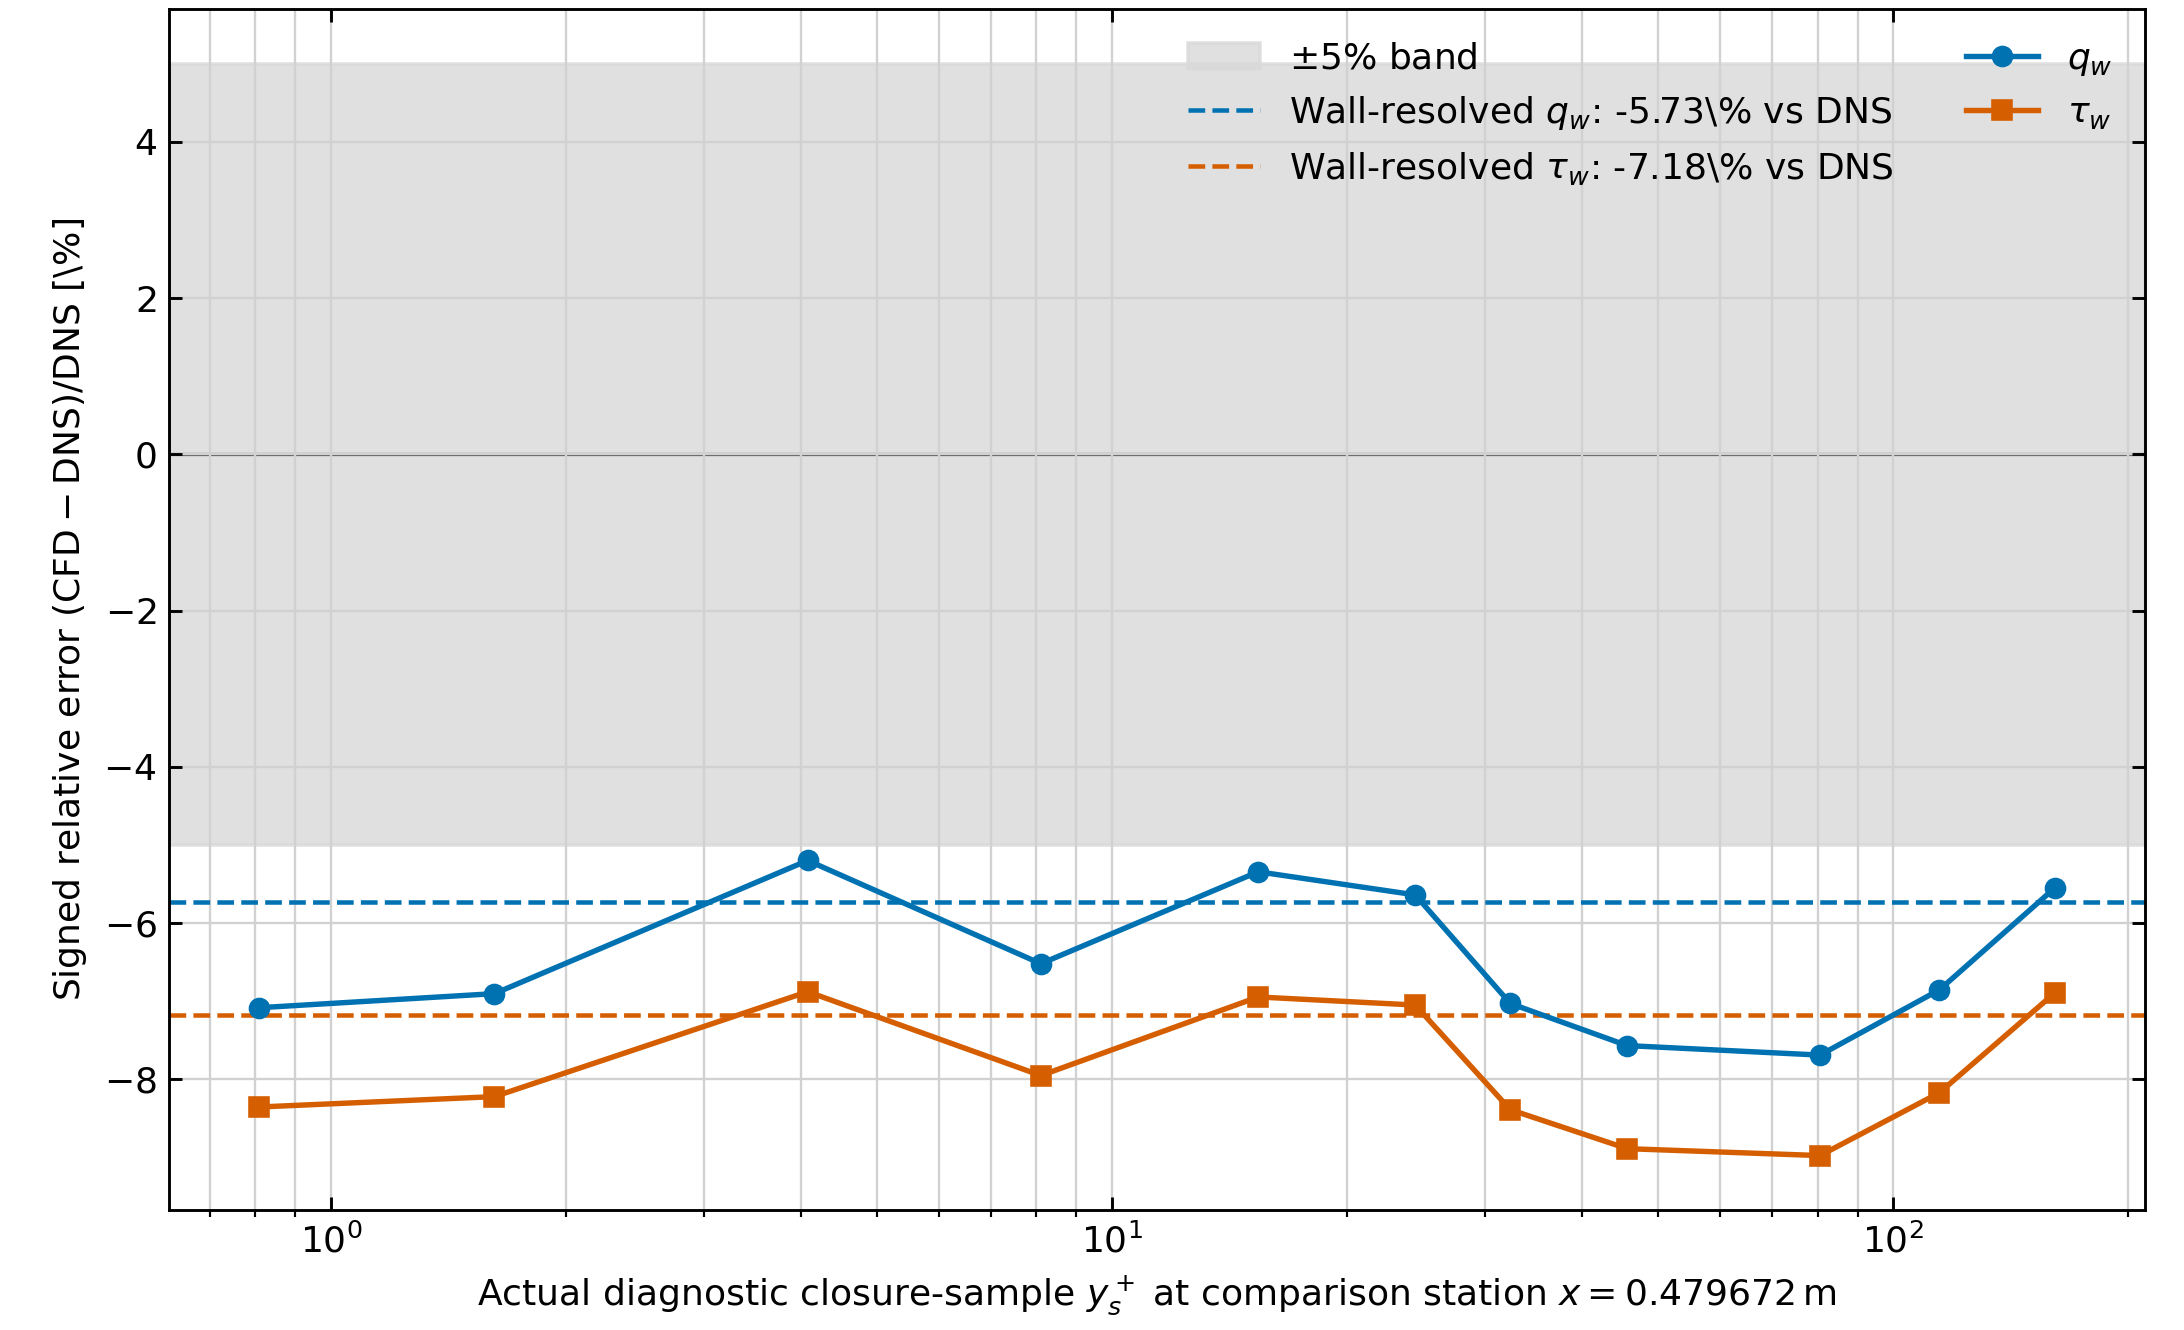
\includegraphics[width=\linewidth,height=.43\textheight,keepaspectratio]{07_Error_Isolation_Results/Figures/WallFunctions/04_3pctMesh_fitted_Li_LowHM3.png}
    \caption[]{(continued) Closures fitted to the wall-resolved SA reference recover its wall heat-flux and shear stress to within approximately $\pm2\%$ on the informed meshes. The baseline discrepancy from DNS remains.}
\end{figure}


\section{Summary}

The main contribution of this work is a novel boundary layer-informed mesh criterion, which is necessary for wall-function simulations of hypersonic cold-wall flat plates. It relates cell spacing to the local profiles, controlling internal-face gradient and transport-coefficient interpolation errors (Sections~\ref{subsec:comparative:zpg:mesh-criterion} and~\ref{subsec:comparative:zpg:informed-mesh}). This criterion also provides the basis for a proposed a-priori mesh-design approach, conditional on estimates of wall loads and wall/edge states (Section~\ref{subsec:comparative:zpg:apriori-mesh}).
\par\medskip

A-priori assessment, independently of coupled CFD, of the Li and Griffin wall-function closures was performed. Across the investigated adiabatic and cold-wall flat plates, relative shear-stress and heat-flux errors are of order \(\pm 10\%\) over the assessed inner-layer sampling range, with some larger deviations in some cases (Section~\ref{subsec:erriso:apriori-results}). This demonstrates promising closure accuracy, although reliance on reconstructed boundary layer-edge quantities introduces an additional sensitivity in CFD (Section~\ref{subsec:wall-functions:griffin:edge-detection}).
\par\medskip

The wall-resolved assessment of the Spalart--Allmaras and \(k\)--\(\omega\) SST turbulence models across twelve zero-pressure-gradient flat-plate cases reinforces existing evidence of their limitations in hypersonic cold-wall flows. Wall heat-flux and shear-stress predictions show substantial, case-dependent discrepancies from DNS, reaching approximately \(\pm 20\%\) (Section~\ref{subsec:comparative:zpg:wr-wall-fluxes}).
\par\medskip

Consistent with previous RANS assessments, both turbulence models were also found to struggle to reproduce the thermal profiles of hypersonic cold-wall boundary layers (Section~\ref{subsec:comparative:zpg:wr-profiles}). These profile discrepancies affect the wall functions that sample the RANS field (Section~\ref{subsec:erriso:rans-profile-influence}). The evidence points to the shared constant turbulent Prandtl number \(Pr_t\) assumption as a plausible cause, although its contribution to wall heat-flux and shear-stress errors has not been isolated (Section~\ref{subsec:comparative:zpg:wr-prandtl}).
\par\medskip

The wall-resolved mesh studies also revisit an existing acoustic-Reynolds-number criterion. Using wall properties and the wall-to-first-cell-centre distance, \(Re_{\mathrm{cell1}}\le1\) provides a more reliable practical resolution guideline than \(y_1^+\le1\) alone for the investigated hypersonic cold-wall cases, particularly with SST (Section~\ref{sec:evaluation:mesh-families-yplus}).

\section{Outlook}
\label{chap:outlook}

\paragraph*{Thermal closure and turbulence modelling}
The similar SA and SST thermal-profile errors and their sensitivity to \(Pr_t\) in Section~\ref{subsec:comparative:zpg:wr-prandtl} make the thermal closure a priority for further research. Variable turbulent Prandtl numbers have long been studied~\cite{kays1994turbulent}, alongside more general turbulent heat-flux closures~\cite{bowersox2009extension}. Huang et al.~\cite{huang2020simulation}, for example, improve cold-wall temperature profiles using an algebraic energy-flux model. Their use of an algebraic momentum model, however, leaves the energy-flux closure's performance with the present SA and SST formulations to be assessed.
\par\medskip

Recent results also show why a variable \(Pr_t\) alone may be insufficient. Cheng et al.~\cite{cheng2026reynolds} attribute most of the reduction in the excessive temperature maximum to revised turbulent kinetic-energy contributions in the governing equations, with their variable-\(Pr_t\) relation provides a smaller additional improvement, but no isolated variable-\(Pr_t\) relation assessment was performed. On the other hand, Hasan et al.~\cite{hasan2025variable} find little effect from replacing \(Pr_t=0.9\) with DNS-derived values in corrected inner-layer calculations with prescribed wall loads. Their inner-layer thermal-profile improvements combine turbulence and energy-source corrections, where wall-load predictions are improved while leaving temperature profiles largely unchanged.
\par\medskip

Compressibility corrections provide another possible direction, but their benefits are also conditional. Allmaras, Johnson and Spalart~\cite[Section~2.2]{AJS2012} reaffirm the same standard SA equation for incompressible and compressible flows, without prescribing an additional compressibility correction. This does not establish its accuracy throughout the hypersonic cold-wall regime. Xue et al.~\cite{xue2024assessment} show that additional SA corrections can improve some predictions while worsening others as compressibility increases. Recent work distinguishing variable-property effects from intrinsic compressibility provides further guidance~\cite{hasan2025intrinsic,hasan2025variable,pecnik2026turbulence}, without establishing a universal correction for the present discrepancies.
\par\medskip

Future work may give interesting insight by varying the thermal closure, momentum-model corrections and energy-equation modelling separately before assessing their combinations. Boundary layer profiles, wall heat-flux and wall shear stress should be evaluated under otherwise consistent conditions. This would test how much of the present discrepancy is attributable to the constant-\(Pr_t\) assumption and which additional changes are required. While at the same time not only the exact turbulence model formulation, but also its coupling to the RANS field needs assessing (ref. Section~\ref{subsec:comparative:zpg:results-assessment}).

\paragraph*{DNS reference data}
The uncertainties and reporting inconsistencies identified with the DNS references of the investigated ZPG flat plates in Section~\ref{sec:evaluation:benchmark-cases} limit conclusions drawn from these widely used benchmarks. Recomputing selected cases and publishing complete flow-field data, including inlet profiles and downstream development, would strengthen their value for future model assessment. Zhang's digitally available profiles illustrate the benefit of accessible reference data. Extending this coverage could also support more controlled thermal-closure tests. Additional cases could also broaden the coverage of wall cooling and compressibility shown in Figure~\ref{fig:evaluation:dns-bq-mtau}.

\paragraph*{Comparison across RANS implementations}
A coordinated comparison and collective summary of the turbulence models variants and their respective code implementations discussed in Section~\ref{subsec:comparative:zpg:results-assessment} could help explain why similar thermal-profile discrepancies coexist with markedly different wall-load predictions. The recurring temperature overshoot in studies using \(Pr_t=0.9\) is a useful starting point. Common meshes, physical models, inflow conditions and matching procedures would help distinguish implementation differences from modelling limitations.

\paragraph*{Boundary layer-informed meshing for engineering applications}
The meshes in Section~\ref{subsec:comparative:zpg:informed-mesh} demonstrate the spacing criterion, but do not optimize the cell count. An engineering algorithm should seek efficient meshes while controlling the relevant internal-face errors, while additionally retaining sufficient leading-edge resolution (Section~\ref{subsec:comparative:zpg:conventional-mesh}). It should permit conventional spacing wherever the local profiles satisfy the criterion, including less restrictive adiabatic or lower-speed conditions. Extension beyond the investigated ZPG flat plates remains necessary. The adaptive wall-functions applicability over the whole boundary layer height (Section~\ref{subsec:erriso:apriori-results}) may facilitate local wall-resolved refinement in regions of complex flow interactions, but this does not automatically establish the wall-functions validity in complex flows.

\paragraph*{A-priori mesh design}
The conditional estimate in Section~\ref{subsec:comparative:zpg:apriori-mesh} demonstrates how the Li wall-function relations can guide mesh design without a resolved reference profile. Future work should revisit this approach with improved closures and assess its sensitivity to estimated wall loads and wall/edge states, particularly near the temperature maximum. This is necessary before treating the estimate as a reliable engineering meshing tool.

\paragraph*{Higher-order discretization}
Higher-order viscous-gradient and transport-coefficient approximations could relax the identified spacing requirement. The compression-corner calculations of Tu et al.~\cite{guohua2012assessment} show that discretization order can substantially affect separation and wall heating. Extending such comparisons to wall-function RANS could establish whether higher-order treatment can improve accuracy or reduce the required cell count.

\paragraph*{Complex flows and the Wang--Craft wall function}
The Wang--Craft formulation merits further investigation because of its reported performance in shock-wave/boundary-layer interactions, including separated flows~\cite{wang2023WF}. The implementation difficulties documented in Section~\ref{sec:wall-functions:wang-craft} should first be resolved, ideally through collaboration with the authors and access to their implementation. Subsequent assessment could thus extend the present error-isolation approach to pressure gradients, separation and complex geometries.

\appendix

% Concise source-based adaptation of the Martin--Duan consistency audit.
\chapter{Reynolds-number inconsistencies in Martin--Duan Part 2}
\label{app:duan-part2-consistency}

This appendix examines the consistency of the Reynolds numbers reported for the Part~2 database~\cite{duan2010direct_part2}, using the published temperature data.

\section{Reynolds-number inconsistency and matching ambiguity}
\label{app:duan:reynolds}

The definitions in Part~2, Section~2.1, use the same edge quantities and momentum thickness:
\begin{equation}
  Re_\theta=\frac{\rho_\delta u_\delta\theta}{\mu_\delta},
  \qquad
  Re_{\delta2}=\frac{\rho_\delta u_\delta\theta}{\mu_w},
  \qquad
  \boxed{\frac{Re_\theta}{Re_{\delta2}}=\frac{\mu_w}{\mu_\delta}}.
  \label{app:duan:eq:ratio}
\end{equation}
For M5T1, the printed \(T_w=T_\delta\) therefore requires \(Re_\theta=Re_{\delta2}\) for any temperature-dependent viscosity law. Instead, Table~1 gives \(1279.1/1538.4=0.83145\ne1\), a \(16.86\%\) deficit relative to unity. This is an inconsistency of the printed row, independent of density, velocity, momentum thickness, or the chosen viscosity exponent.

The other cases also fail a common power-law test. Part~2 inherits the power-law viscosity model stated in Part~1~\cite[Section~2]{martin2007direct_Part1}. Writing \(\mu=CT^\omega\), Equation~\eqref{app:duan:eq:ratio} requires \(Re_\theta/Re_{\delta2}=(T_w/T_\delta)^\omega\). The implied exponents \(\omega=\ln(Re_\theta/Re_{\delta2})/\ln(T_w/T_\delta)\) in Table~\ref{app:duan:tab:ratios} have no common intersection even after allowing for rounding of the printed entries.

\begin{table}[H]
  \centering
  \caption{Part~2 Table~1 ratio test. Intervals allow half a unit in each last printed digit; endpoints are rounded outward.}
  \label{app:duan:tab:ratios}
  \small
  \begin{tabular}{@{}l
    S[table-format=1.2]
    S[table-format=4.1]
    S[table-format=4.1]
    S[table-format={[}1.4]@{,\,}S[table-format=1.4{]}]@{}}
    \toprule
    Case & {\(T_w/T_\delta\)} & {\(Re_\theta\)} & {\(Re_{\delta2}\)} & \multicolumn{2}{c@{}}{Implied \(\omega\) interval} \\
    \midrule
    M5T2 & 1.90 & 2300.2 & 1521.5 & {[}0.6412 & 0.6467{]} \\
    M5T3 & 2.89 & 3011.6 & 1524.7 & {[}0.6402 & 0.6425{]} \\
    M5T4 & 3.74 & 3819.3 & 1526.4 & {[}0.6945 & 0.6961{]} \\
    M5T5 & 5.40 & 4840.5 & 1536.8 & {[}0.6799 & 0.6808{]} \\
    \bottomrule
  \end{tabular}
\end{table}

A separate check illustrates the dimensional ambiguity. Part~1's M5~\cite[Table~2]{martin2007direct_Part1} and Part~2's M5T5~\cite[Table~1]{duan2010direct_part2} have effectively identical printed edge states, while \(\theta\) changes from \(0.657\) to \(0.655\,\mathrm{mm}\). With the same edge viscosity, \(Re_\theta\propto\theta\), giving \(6225(0.655/0.657)=6206.1\), whereas Part~2 prints \(4840.5\), approximately \(22.0\%\) lower. Temporal evolution alone cannot reconcile these columns while preserving the reported edge state and viscosity model.

Accordingly, this thesis retains the published \(Re_{\delta2}\approx1530\) values as the authors' intended matching targets~\cite[Section~2.1]{duan2010direct_part2}. They are nominal reference labels, not independently verified dimensional reconstructions. The tables do not determine unique corrected Reynolds numbers or establish whether the mismatch reflects transport conventions, post-processing, or sampling. For M5T1, the accepted \(T_w=T_\delta\) requires equality of the two Reynolds numbers; additionally retaining \(Re_{\delta2}=1538.4\) would give \(Re_\theta=1538.4\). This is conditional on that matching target, rather than an independent reconstruction of both Reynolds numbers.

\chapter{Wall-resolved mesh convergence}
\label{app:zpg:mesh-convergence}

The following wall-normal mesh studies supplement
Section~\ref{sec:evaluation:mesh-families-yplus} for all twelve ZPG cases,
including Huang's three stations. Coefficients are evaluated at each mesh's
\(Re_{\delta2}\)-matched station. Dashed lines show E\c{c}a--Hoekstra
extrapolations from the four finest meshes; shaded bands mark
\(\pm1\%\) of each extrapolated value and do not measure agreement with DNS.

\section{Martin--Duan Parts 2 and 4}

\begin{figure}[!htbp]
    \centering
    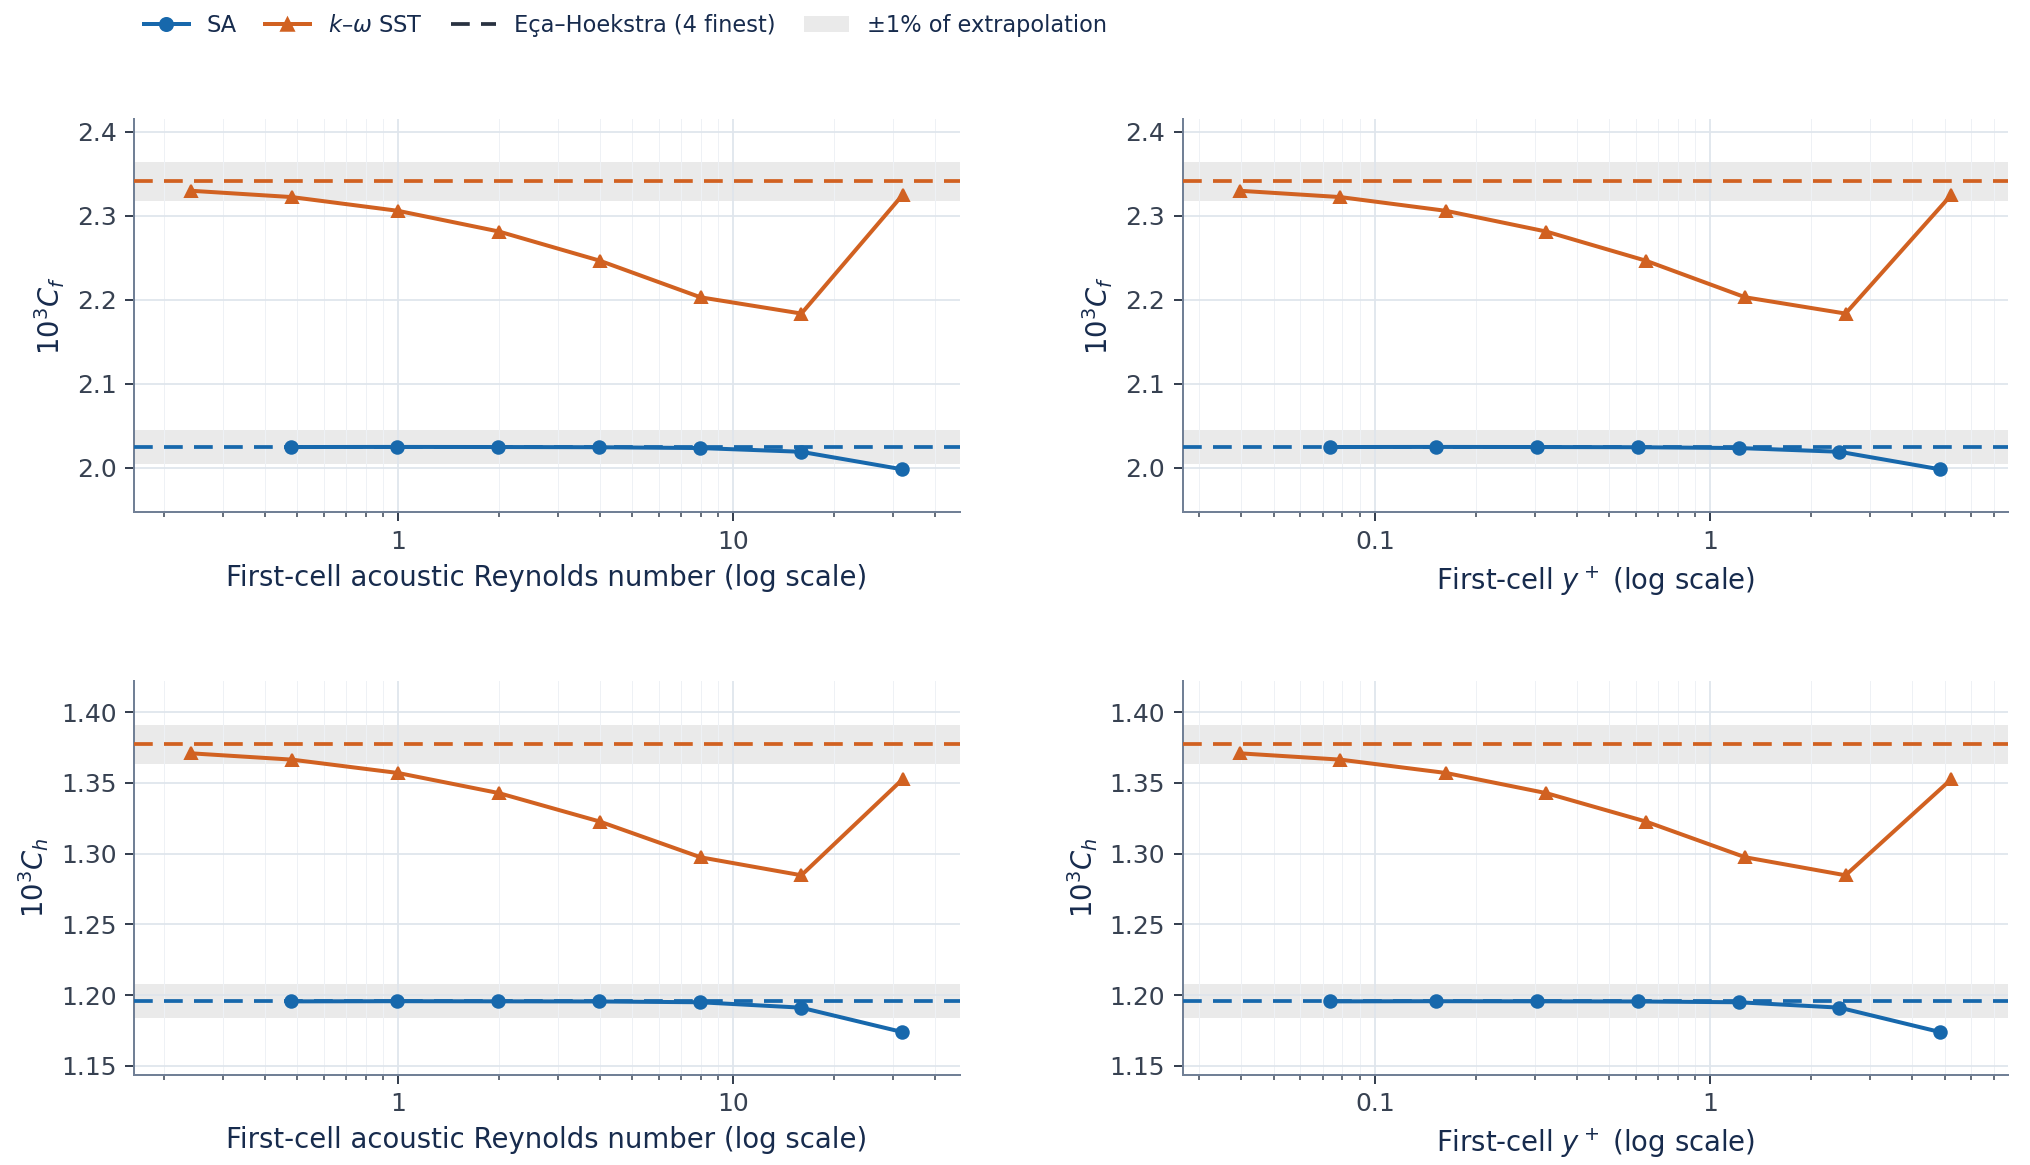
\includegraphics[width=\linewidth]{06_Eval_Methodology/06_Figures/Appendix/Martin_Duan_2_M5T1_Re_delta2.png}
    \caption[Martin--Duan Part~2 M5T1: wall-normal mesh sensitivity]{Wall-normal mesh sensitivity for Martin--Duan Part~2 M5T1, comparing Spalart--Allmaras and \(k\)--\(\omega\) SST. Skin-friction coefficient \(C_f\) (top) and Stanton number \(C_h\) (bottom) versus first-cell acoustic Reynolds number (left) and first-cell \(y^+\) (right) at the matched \(Re_{\delta2}\) = 1538.4 station. Dashed line represents E\c{c}a--Hoekstra extrapolations from the four finest mesh results; shaded bands mark \(\pm1\%\) of each extrapolated value.}
    \label{fig:app:zpg:mesh:M5T1}
\end{figure}

\begin{figure}[!htbp]
    \centering
    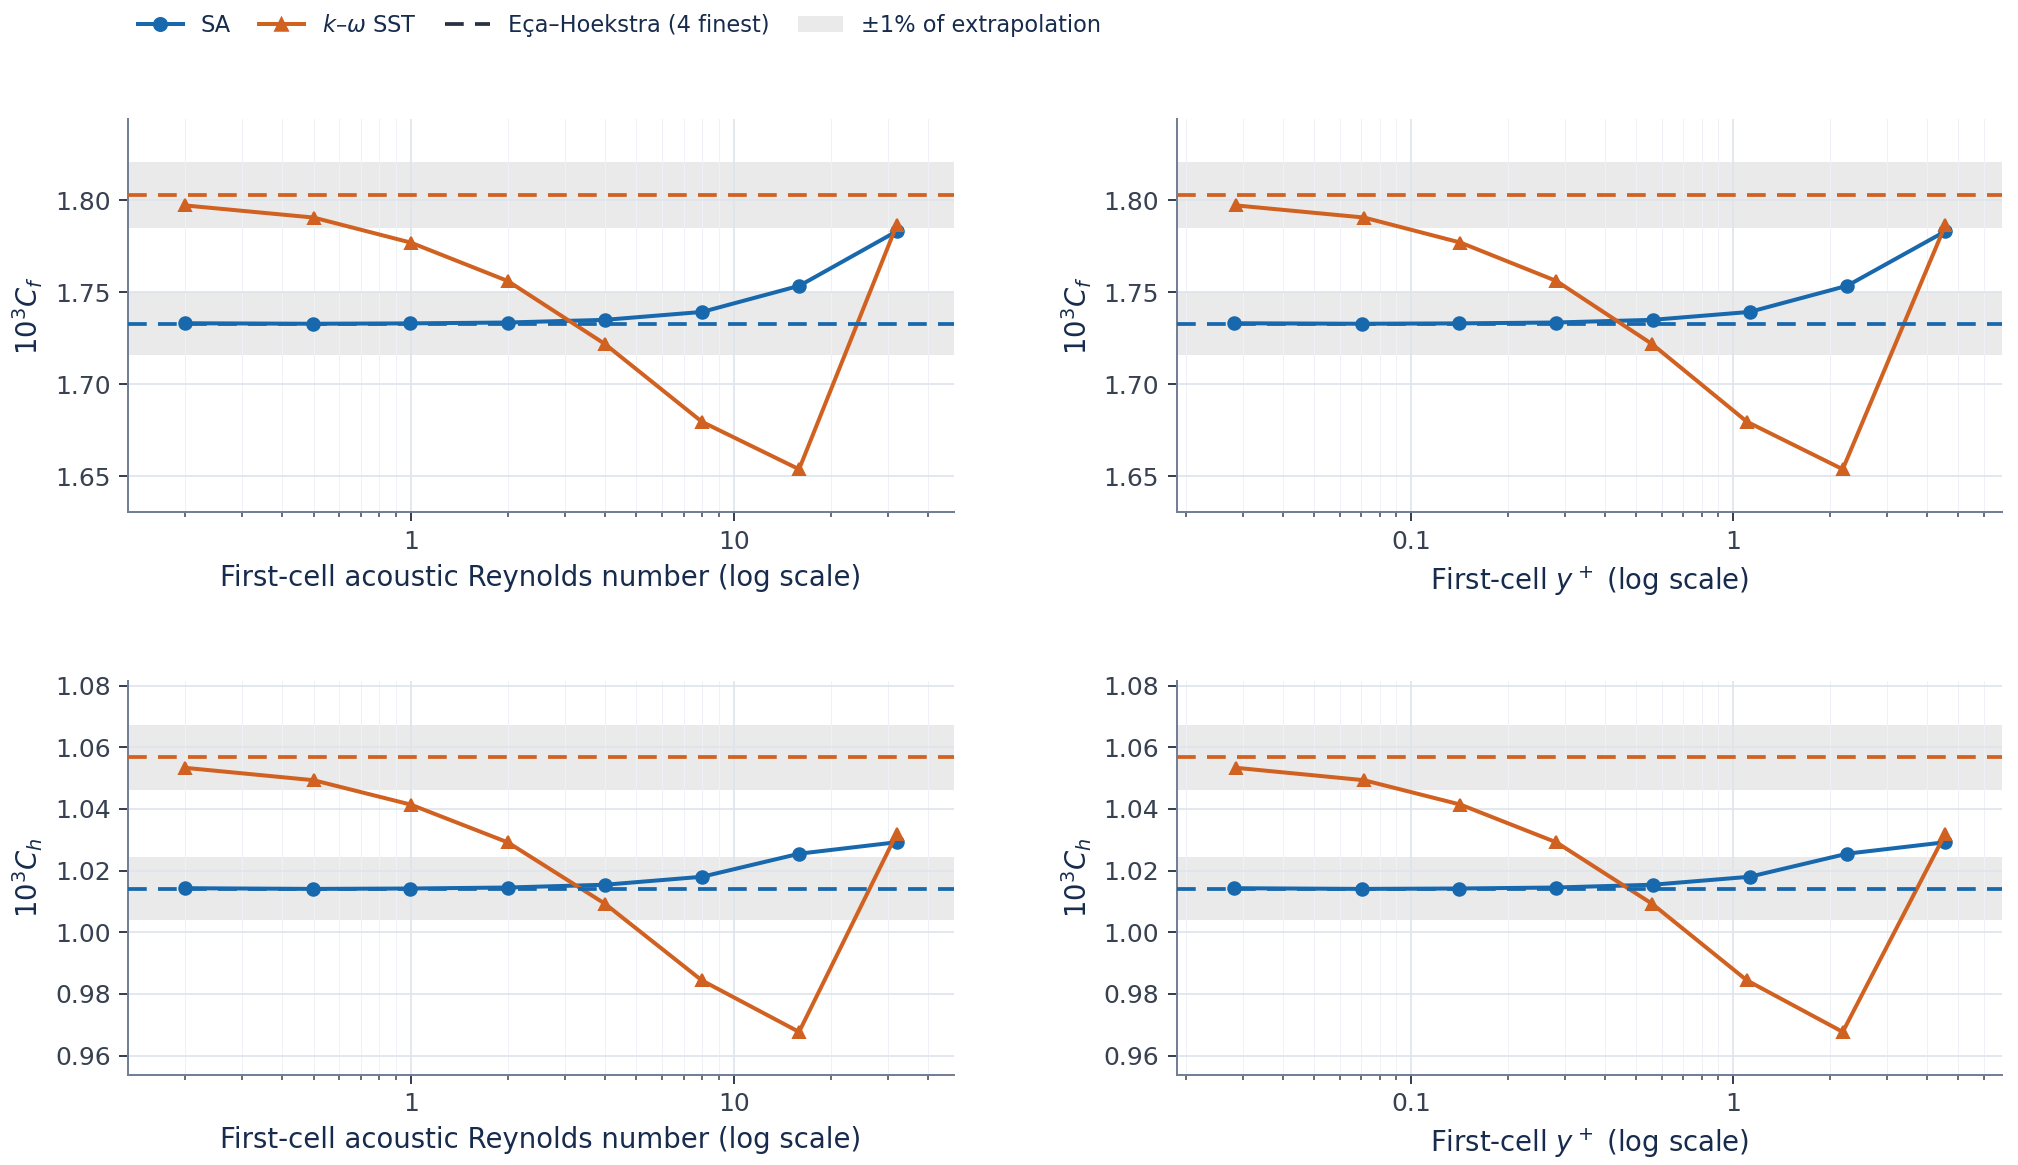
\includegraphics[width=\linewidth]{06_Eval_Methodology/06_Figures/Appendix/Martin_Duan_2_M5T2_Re_delta2.png}
    \caption[Martin--Duan Part~2 M5T2: wall-normal mesh sensitivity]{Wall-normal mesh sensitivity for Martin--Duan Part~2 M5T2, comparing Spalart--Allmaras and \(k\)--\(\omega\) SST. Skin-friction coefficient \(C_f\) (top) and Stanton number \(C_h\) (bottom) versus first-cell acoustic Reynolds number (left) and first-cell \(y^+\) (right) at the matched \(Re_{\delta2}\) = 1521.5 station. Dashed line represents E\c{c}a--Hoekstra extrapolations from the four finest mesh results; shaded bands mark \(\pm1\%\) of each extrapolated value.}
    \label{fig:app:zpg:mesh:M5T2}
\end{figure}

\begin{figure}[!htbp]
    \centering
    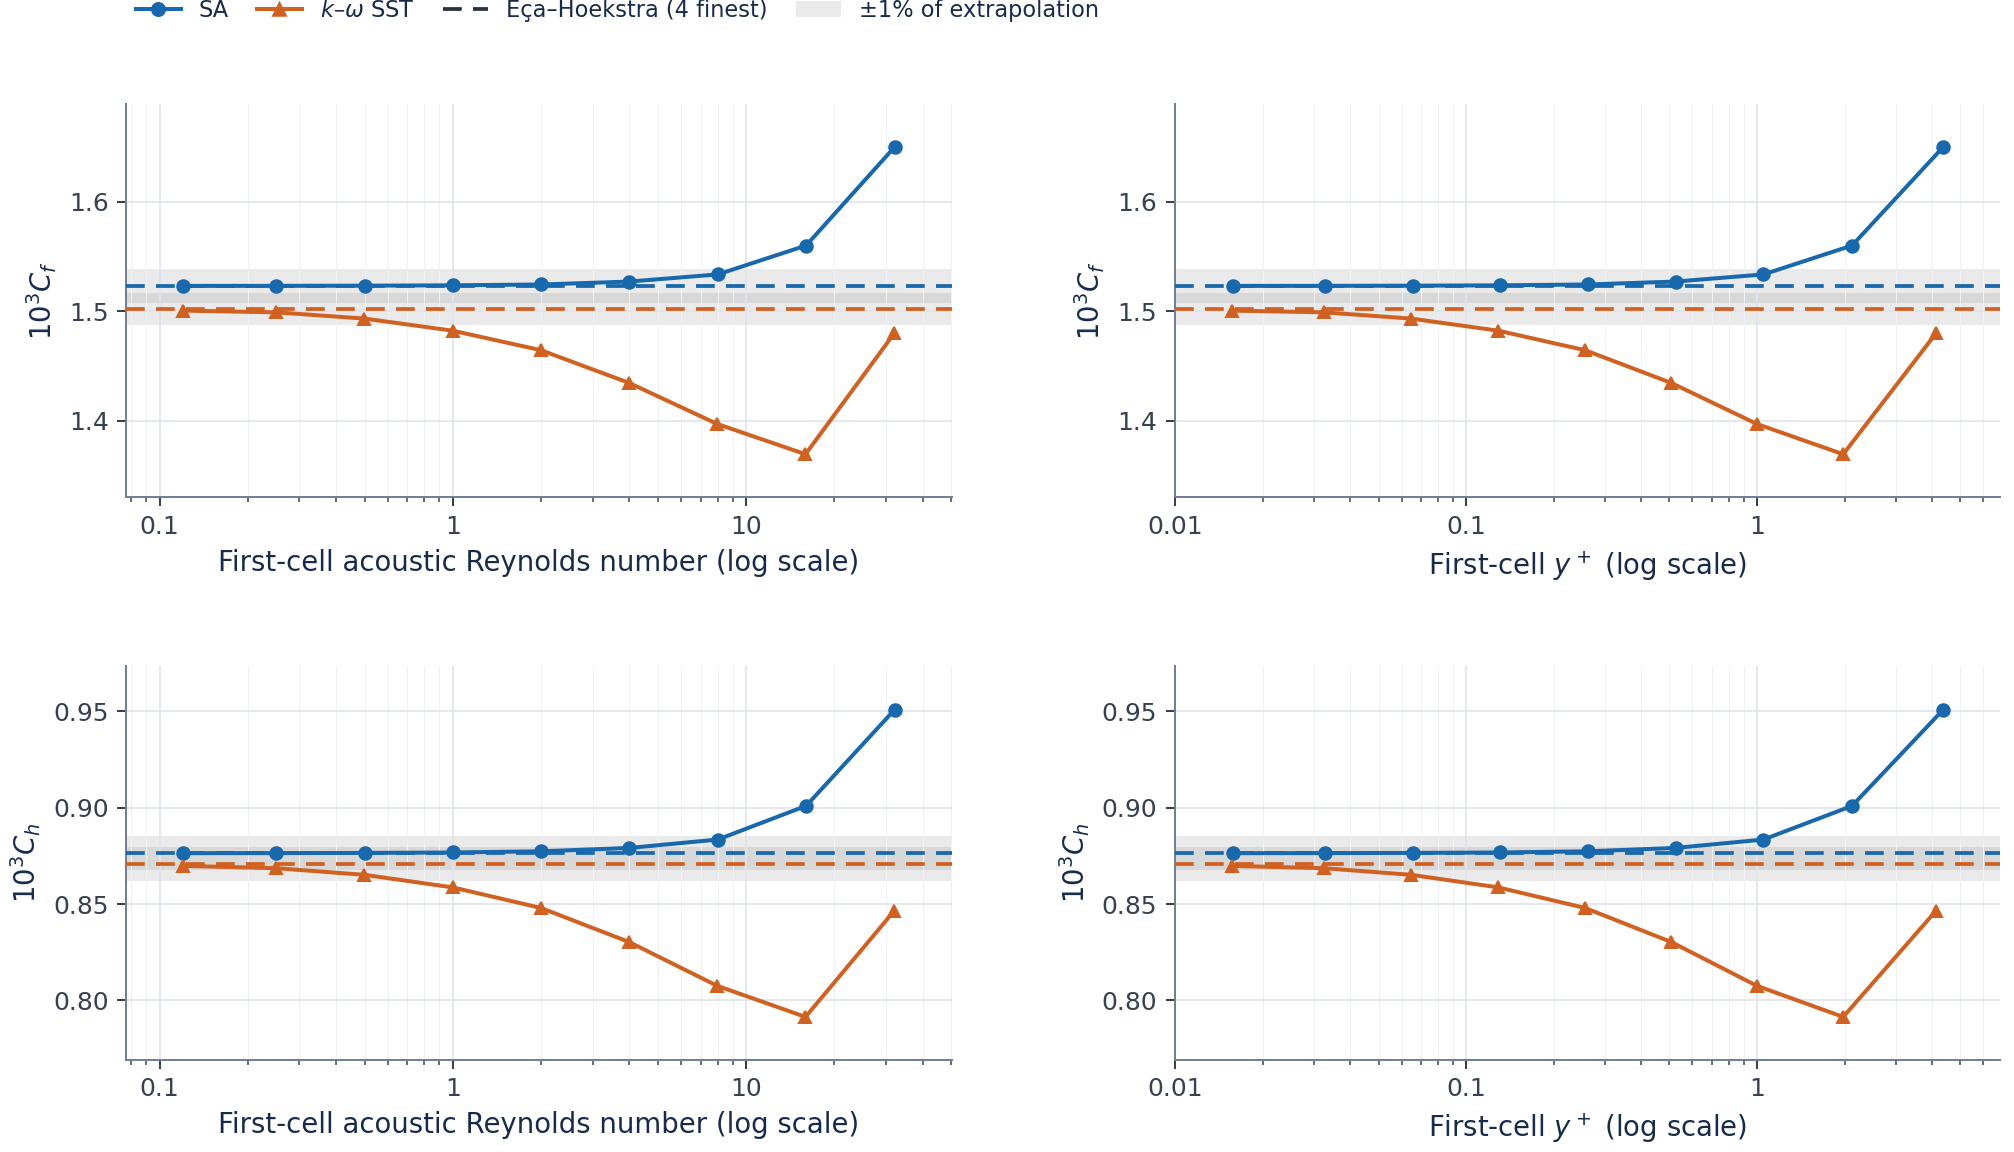
\includegraphics[width=\linewidth]{06_Eval_Methodology/06_Figures/Appendix/Martin_Duan_2_M5T3_Re_delta2.png}
    \caption[Martin--Duan Part~2 M5T3: wall-normal mesh sensitivity]{Wall-normal mesh sensitivity for Martin--Duan Part~2 M5T3, comparing Spalart--Allmaras and \(k\)--\(\omega\) SST. Skin-friction coefficient \(C_f\) (top) and Stanton number \(C_h\) (bottom) versus first-cell acoustic Reynolds number (left) and first-cell \(y^+\) (right) at the matched \(Re_{\delta2}\) = 1524.7 station. Dashed line represents E\c{c}a--Hoekstra extrapolations from the four finest mesh results; shaded bands mark \(\pm1\%\) of each extrapolated value.}
    \label{fig:app:zpg:mesh:M5T3}
\end{figure}

\begin{figure}[!htbp]
    \centering
    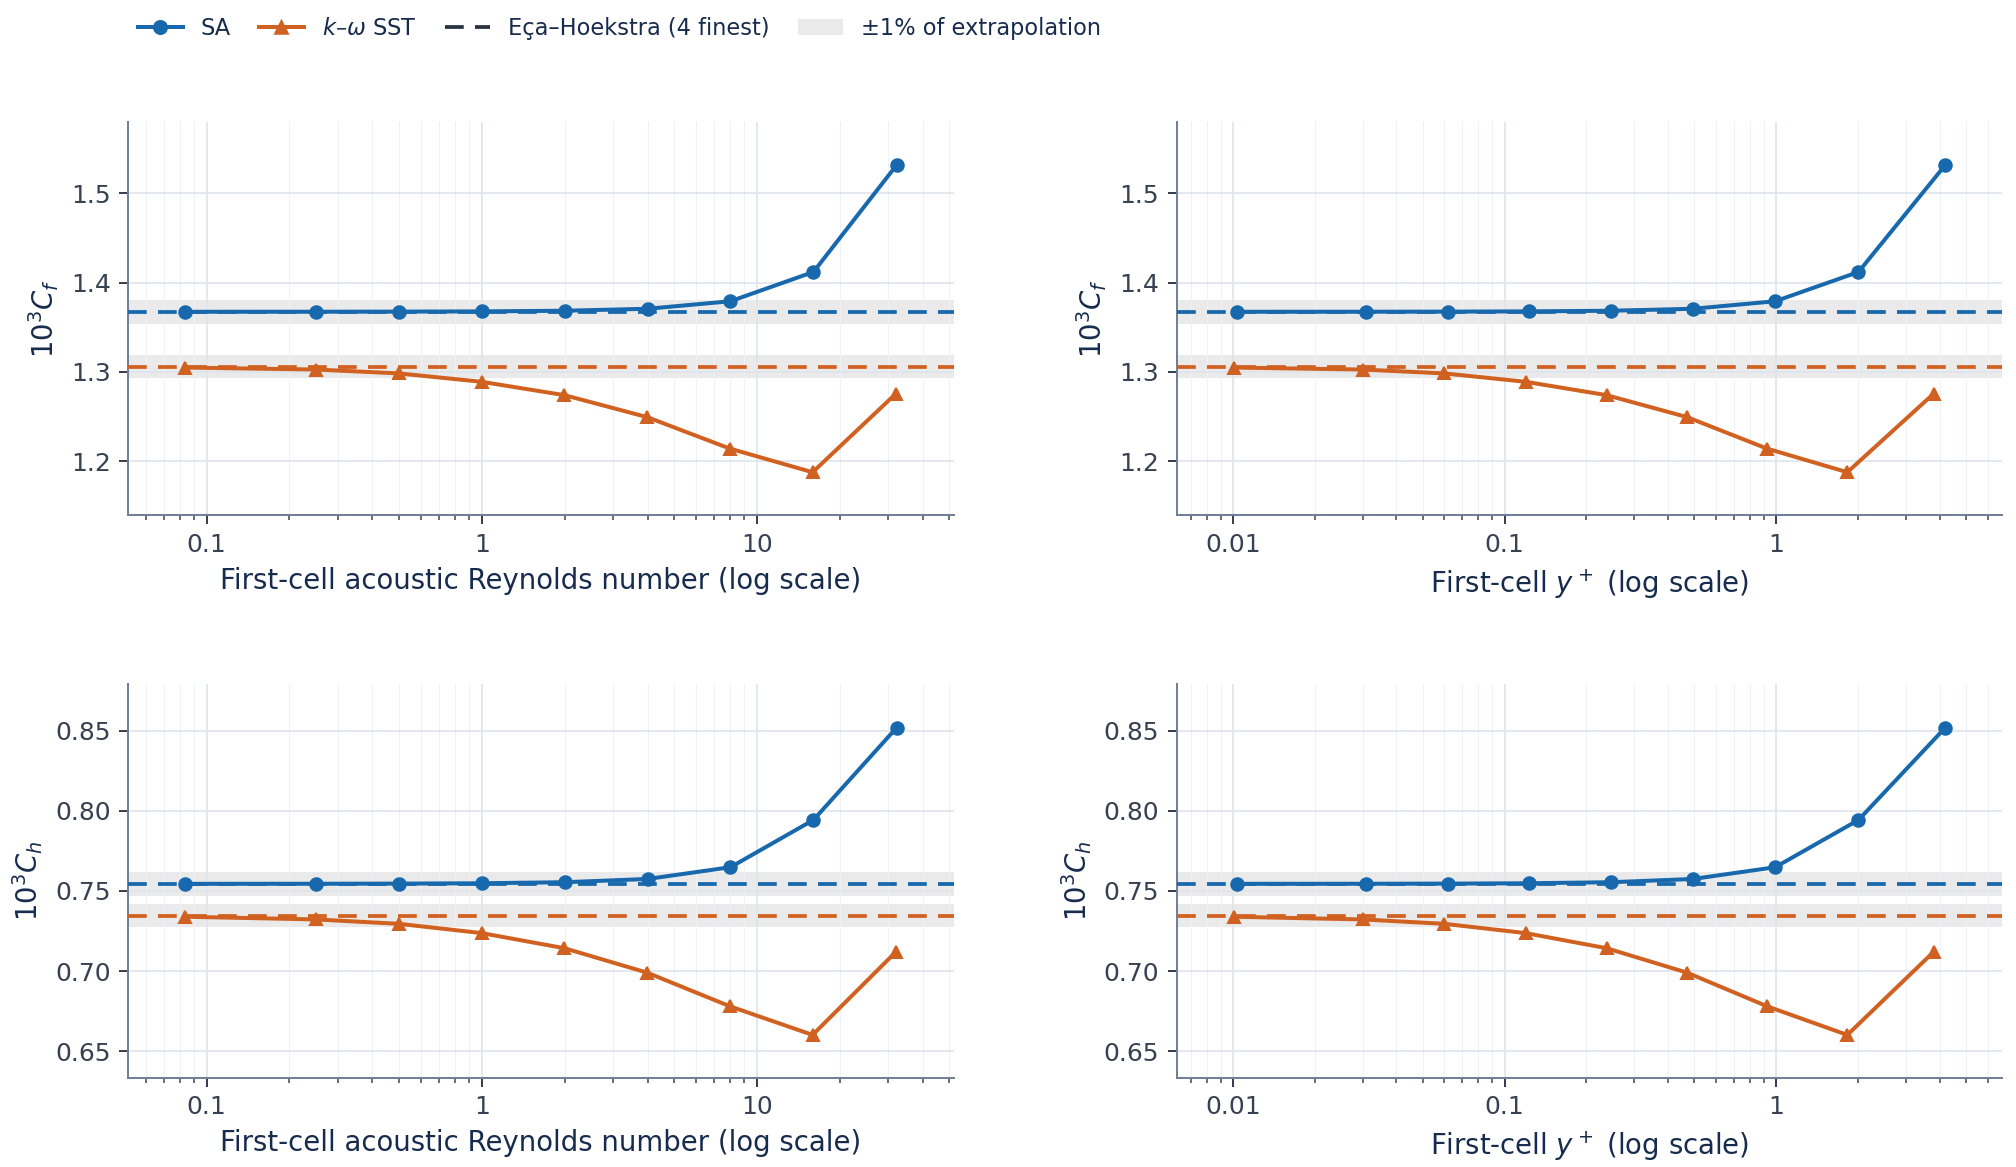
\includegraphics[width=\linewidth]{06_Eval_Methodology/06_Figures/Appendix/Martin_Duan_2_M5T4_Re_delta2.png}
    \caption[Martin--Duan Part~2 M5T4: wall-normal mesh sensitivity]{Wall-normal mesh sensitivity for Martin--Duan Part~2 M5T4, comparing Spalart--Allmaras and \(k\)--\(\omega\) SST. Skin-friction coefficient \(C_f\) (top) and Stanton number \(C_h\) (bottom) versus first-cell acoustic Reynolds number (left) and first-cell \(y^+\) (right) at the matched \(Re_{\delta2}\) = 1526.4 station. Dashed line represents E\c{c}a--Hoekstra extrapolations from the four finest mesh results; shaded bands mark \(\pm1\%\) of each extrapolated value.}
    \label{fig:app:zpg:mesh:M5T4}
\end{figure}

\begin{figure}[!htbp]
    \centering
    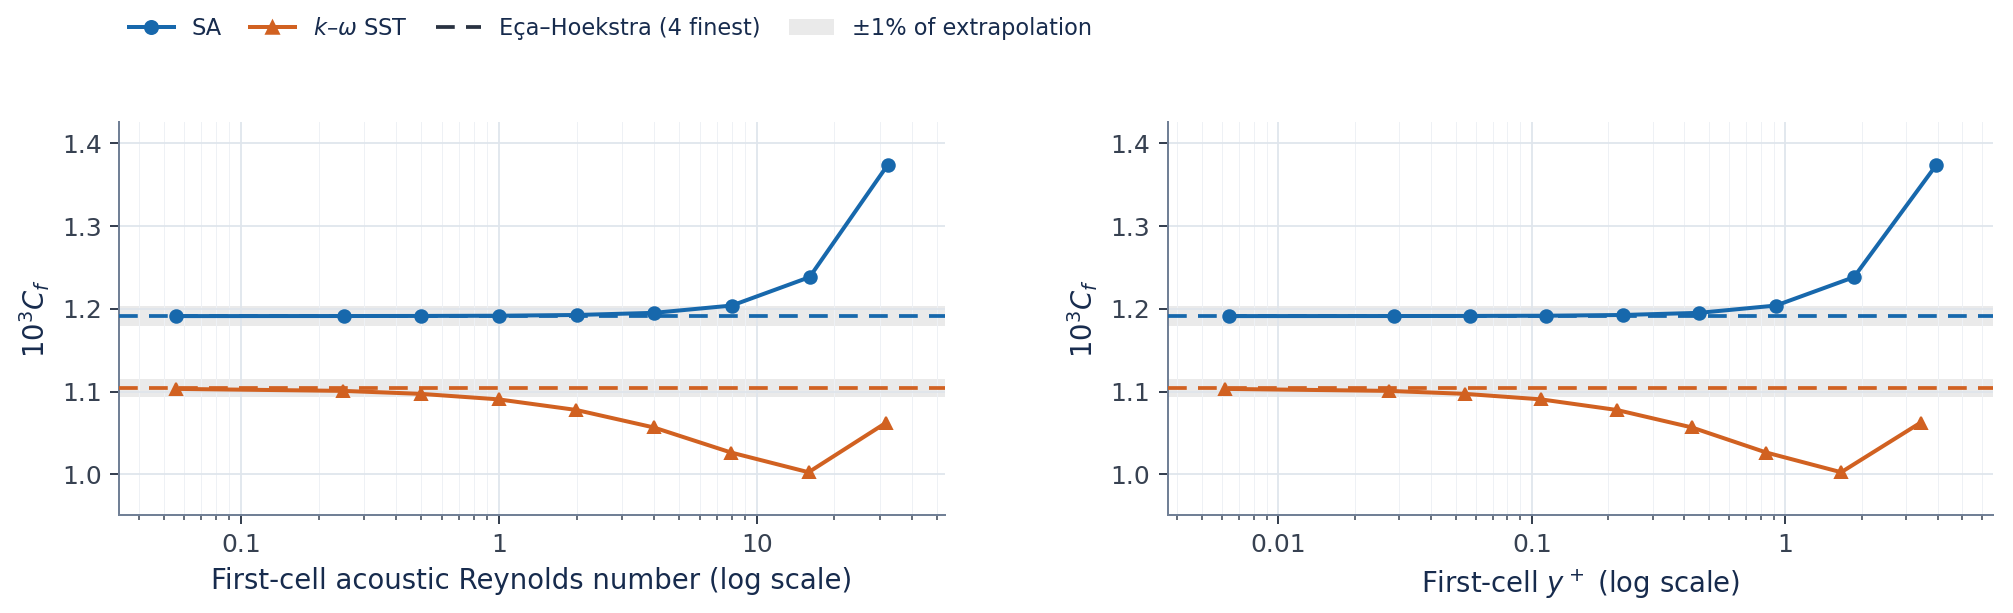
\includegraphics[width=\linewidth]{06_Eval_Methodology/06_Figures/Appendix/Martin_Duan_2_M5T5_Re_delta2.png}
    \caption[Martin--Duan Part~2 M5T5: wall-normal mesh sensitivity]{Wall-normal mesh sensitivity for Martin--Duan Part~2 M5T5, comparing Spalart--Allmaras and \(k\)--\(\omega\) SST. Skin-friction coefficient \(C_f\) versus first-cell acoustic Reynolds number (left) and first-cell \(y^+\) (right) at the matched \(Re_{\delta2}\) = 1536.8 station. Dashed line represents E\c{c}a--Hoekstra extrapolations from the four finest mesh results; shaded bands mark \(\pm1\%\) of each extrapolated value. Heat-transfer is not assessed for this adiabatic case.}
    \label{fig:app:zpg:mesh:M5T5}
\end{figure}

\begin{figure}[!htbp]
    \centering
    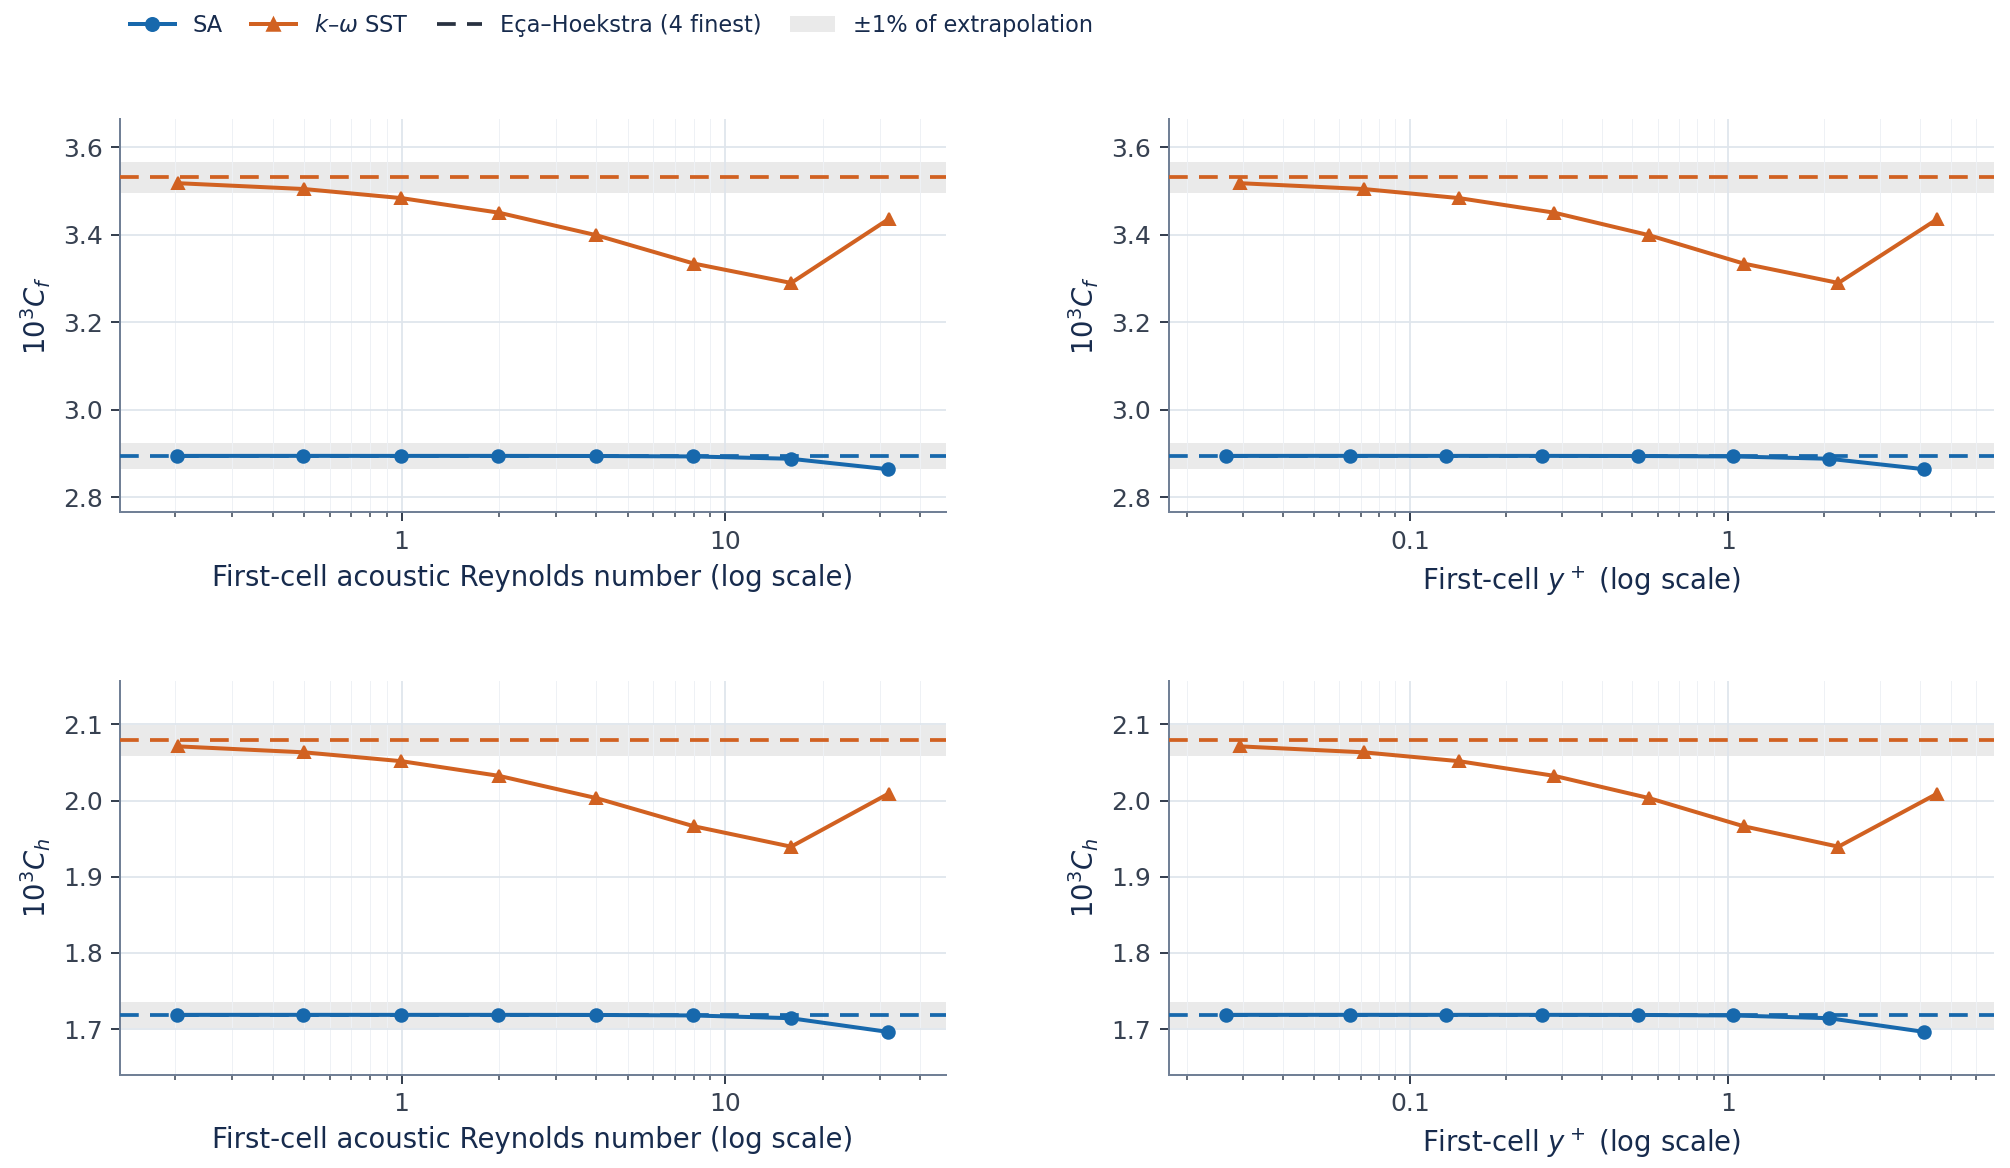
\includegraphics[width=\linewidth]{06_Eval_Methodology/06_Figures/Appendix/Martin_Duan_4_LowH_M3_Re_delta2.png}
    \caption[Martin--Duan Part~4 LowH\_M3: wall-normal mesh sensitivity]{Wall-normal mesh sensitivity for Martin--Duan Part~4 LowH\_M3, comparing Spalart--Allmaras and \(k\)--\(\omega\) SST. Skin-friction coefficient \(C_f\) (top) and Stanton number \(C_h\) (bottom) versus first-cell acoustic Reynolds number (left) and first-cell \(y^+\) (right) at the matched \(Re_{\delta2}\) = 1554.5 station. Dashed line represents E\c{c}a--Hoekstra extrapolations from the four finest mesh results; shaded bands mark \(\pm1\%\) of each extrapolated value.}
    \label{fig:app:zpg:mesh:LowH-M3}
\end{figure}

\clearpage
\section{Zhang cases}

\begin{figure}[!htbp]
    \centering
    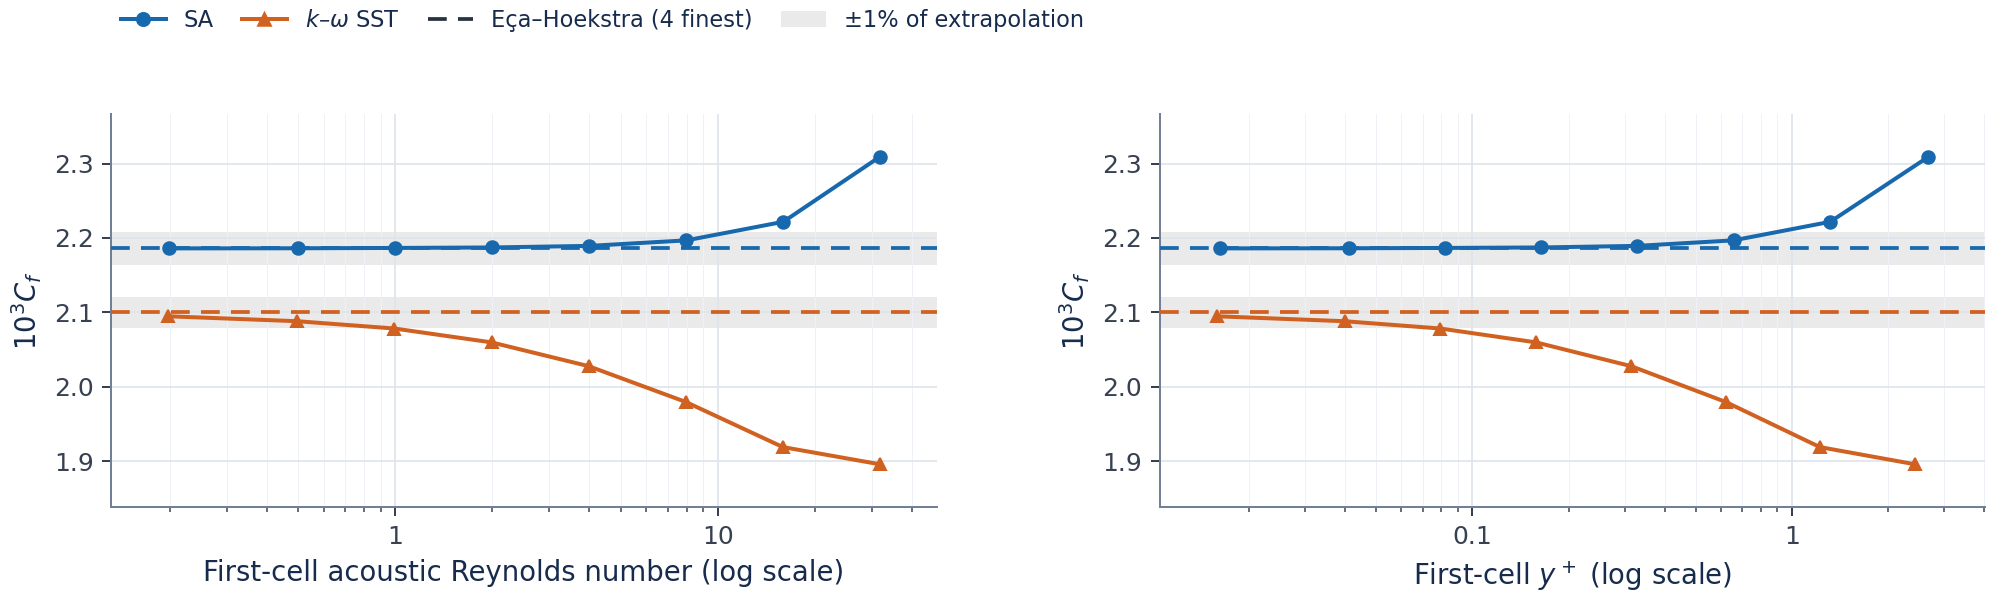
\includegraphics[width=\linewidth]{06_Eval_Methodology/06_Figures/Appendix/Zhang_M2p5_Re_delta2.png}
    \caption[Zhang M2p5: wall-normal mesh sensitivity]{Wall-normal mesh sensitivity for Zhang M2p5, comparing Spalart--Allmaras and \(k\)--\(\omega\) SST. Skin-friction coefficient \(C_f\) versus first-cell acoustic Reynolds number (left) and first-cell \(y^+\) (right) at the matched \(Re_{\delta2}\) = 1657 station. Dashed line represents E\c{c}a--Hoekstra extrapolations from the four finest mesh results; shaded bands mark \(\pm1\%\) of each extrapolated value. Heat-transfer is not assessed for this adiabatic case.}
    \label{fig:app:zpg:mesh:M2p5}
\end{figure}

\begin{figure}[!htbp]
    \centering
    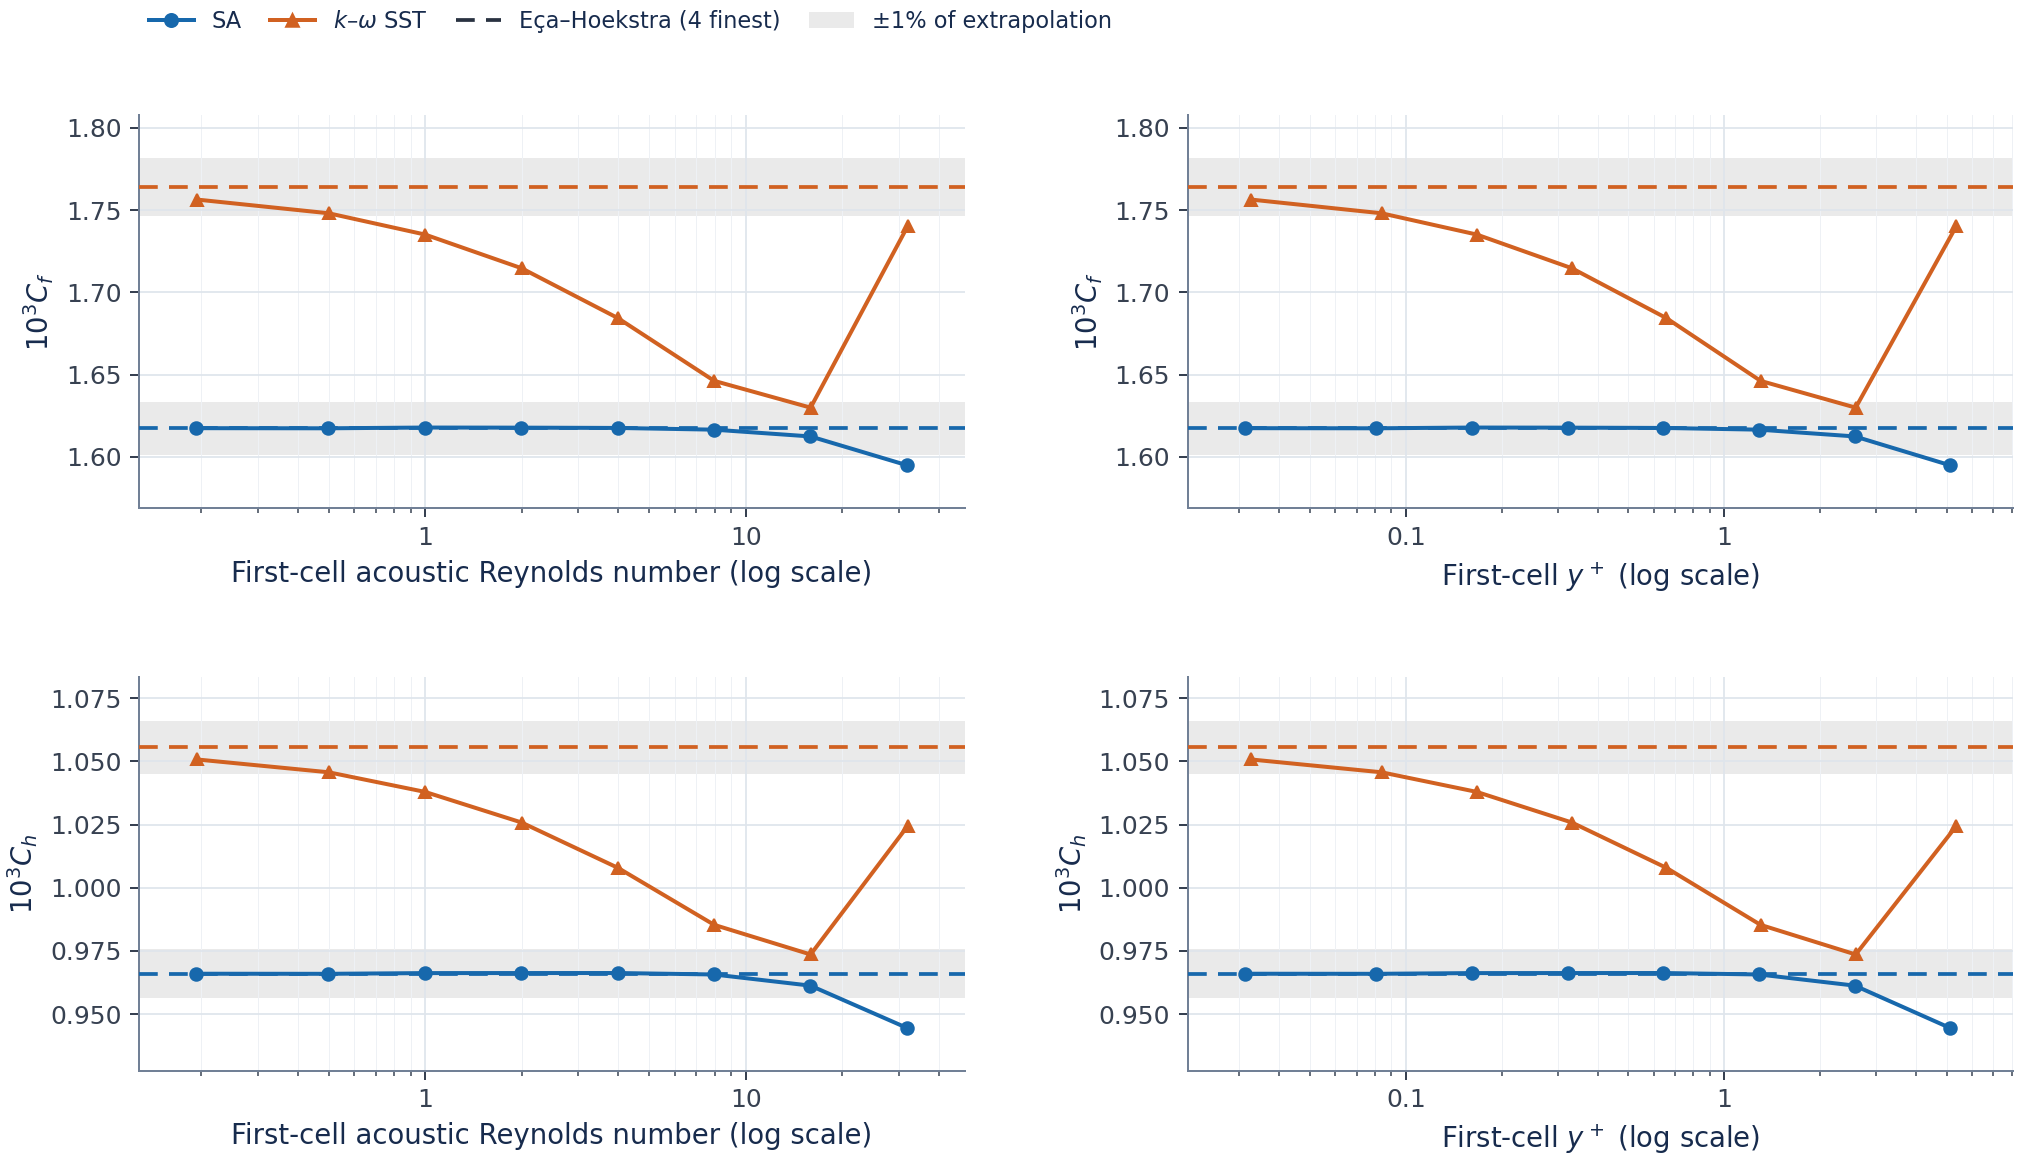
\includegraphics[width=\linewidth]{06_Eval_Methodology/06_Figures/Appendix/Zhang_M6Tw025_Re_delta2.png}
    \caption[Zhang M6Tw025: wall-normal mesh sensitivity]{Wall-normal mesh sensitivity for Zhang M6Tw025, comparing Spalart--Allmaras and \(k\)--\(\omega\) SST. Skin-friction coefficient \(C_f\) (top) and Stanton number \(C_h\) (bottom) versus first-cell acoustic Reynolds number (left) and first-cell \(y^+\) (right) at the matched \(Re_{\delta2}\) = 1135 station. Dashed line represents E\c{c}a--Hoekstra extrapolations from the four finest mesh results; shaded bands mark \(\pm1\%\) of each extrapolated value.}
    \label{fig:app:zpg:mesh:M6Tw025}
\end{figure}

\begin{figure}[!htbp]
    \centering
    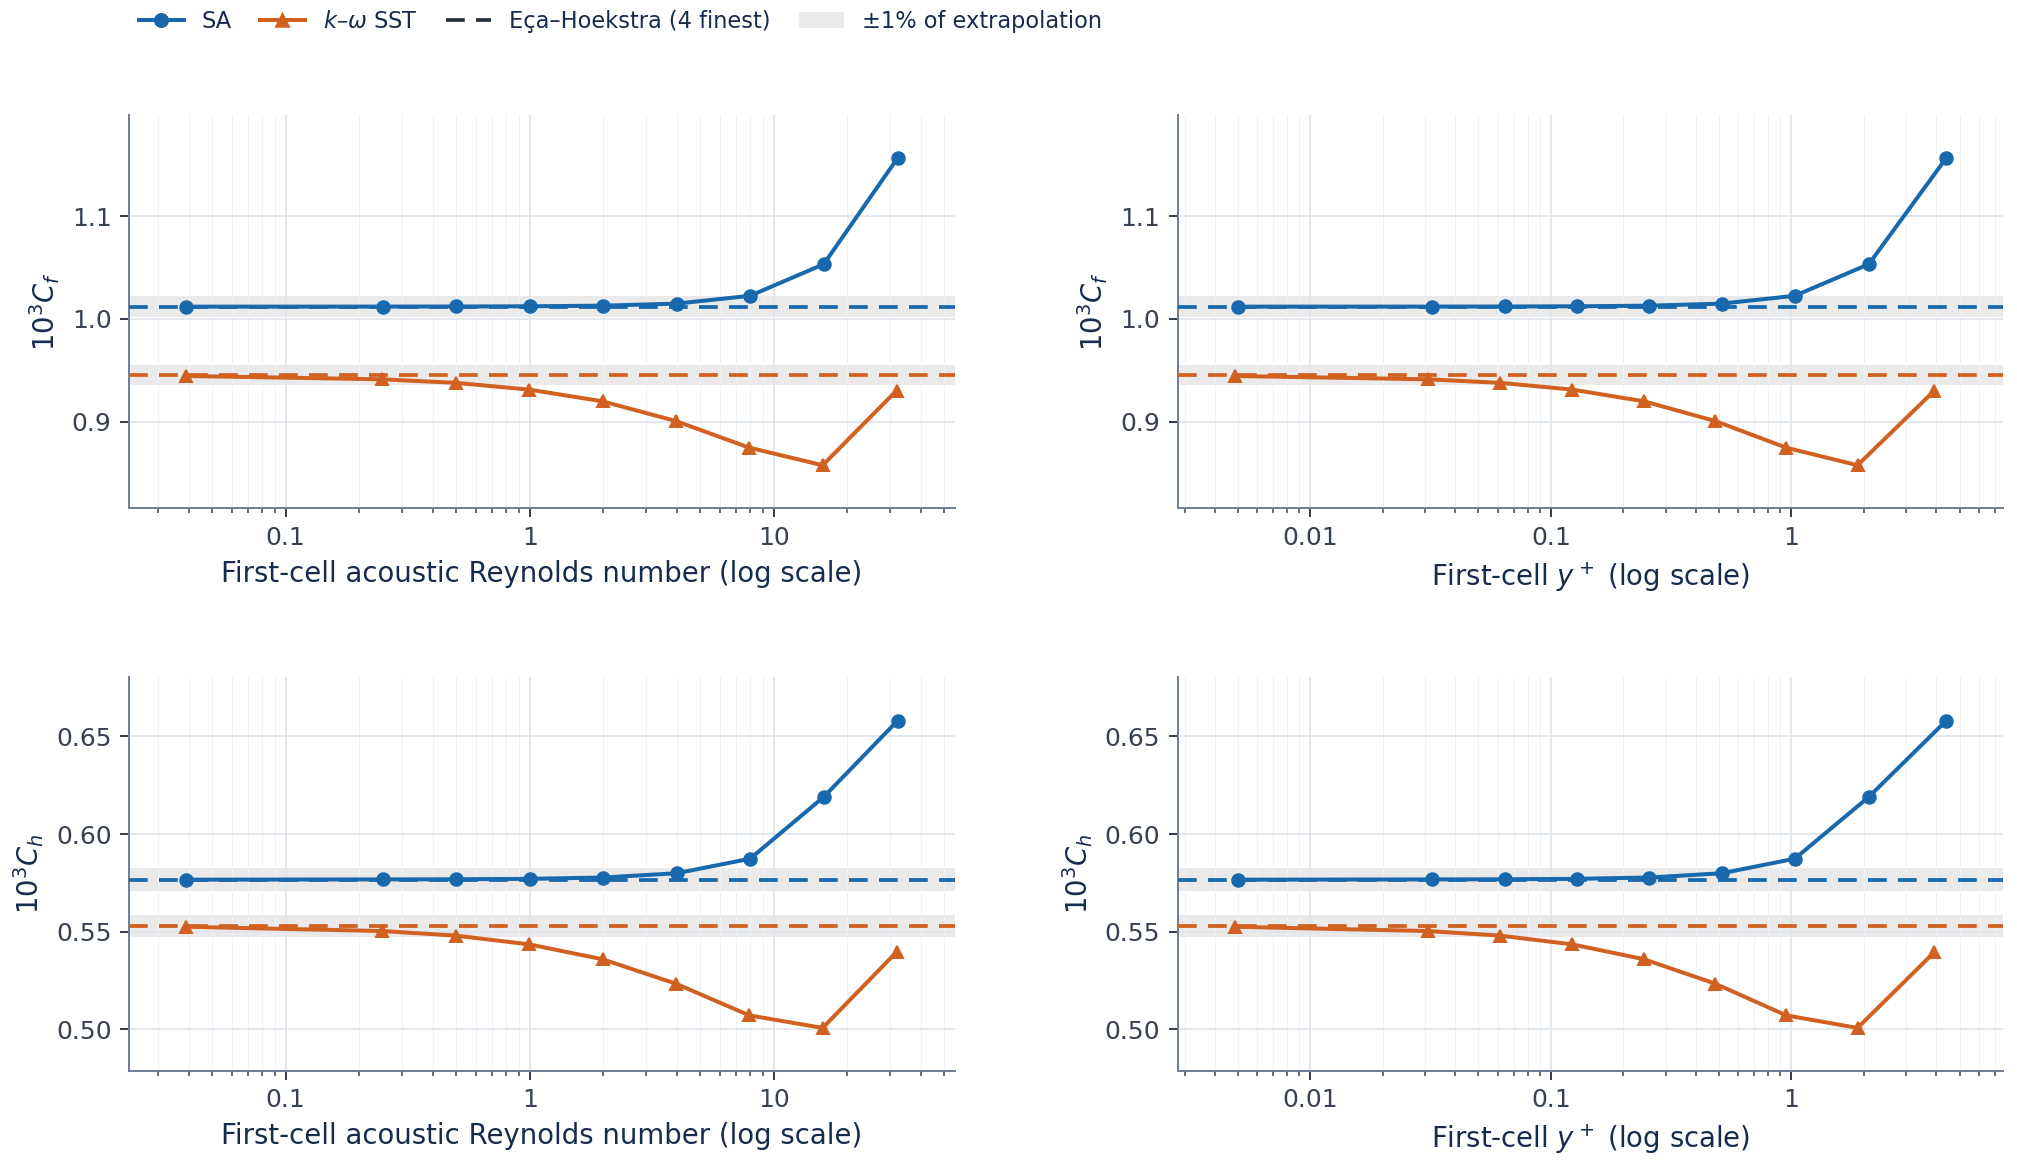
\includegraphics[width=\linewidth]{06_Eval_Methodology/06_Figures/Appendix/Zhang_M6Tw076_Re_delta2.png}
    \caption[Zhang M6Tw076: wall-normal mesh sensitivity]{Wall-normal mesh sensitivity for Zhang M6Tw076, comparing Spalart--Allmaras and \(k\)--\(\omega\) SST. Skin-friction coefficient \(C_f\) (top) and Stanton number \(C_h\) (bottom) versus first-cell acoustic Reynolds number (left) and first-cell \(y^+\) (right) at the matched \(Re_{\delta2}\) = 1746 station. Dashed line represents E\c{c}a--Hoekstra extrapolations from the four finest mesh results; shaded bands mark \(\pm1\%\) of each extrapolated value. The \(C_h\) curves document mesh sensitivity only; the reference-data limitations in Section~\ref{sec:evaluation:benchmark-cases} preclude their use for quantitative heat-flux validation against DNS.}
    \label{fig:app:zpg:mesh:M6Tw076}
\end{figure}

\begin{figure}[!htbp]
    \centering
    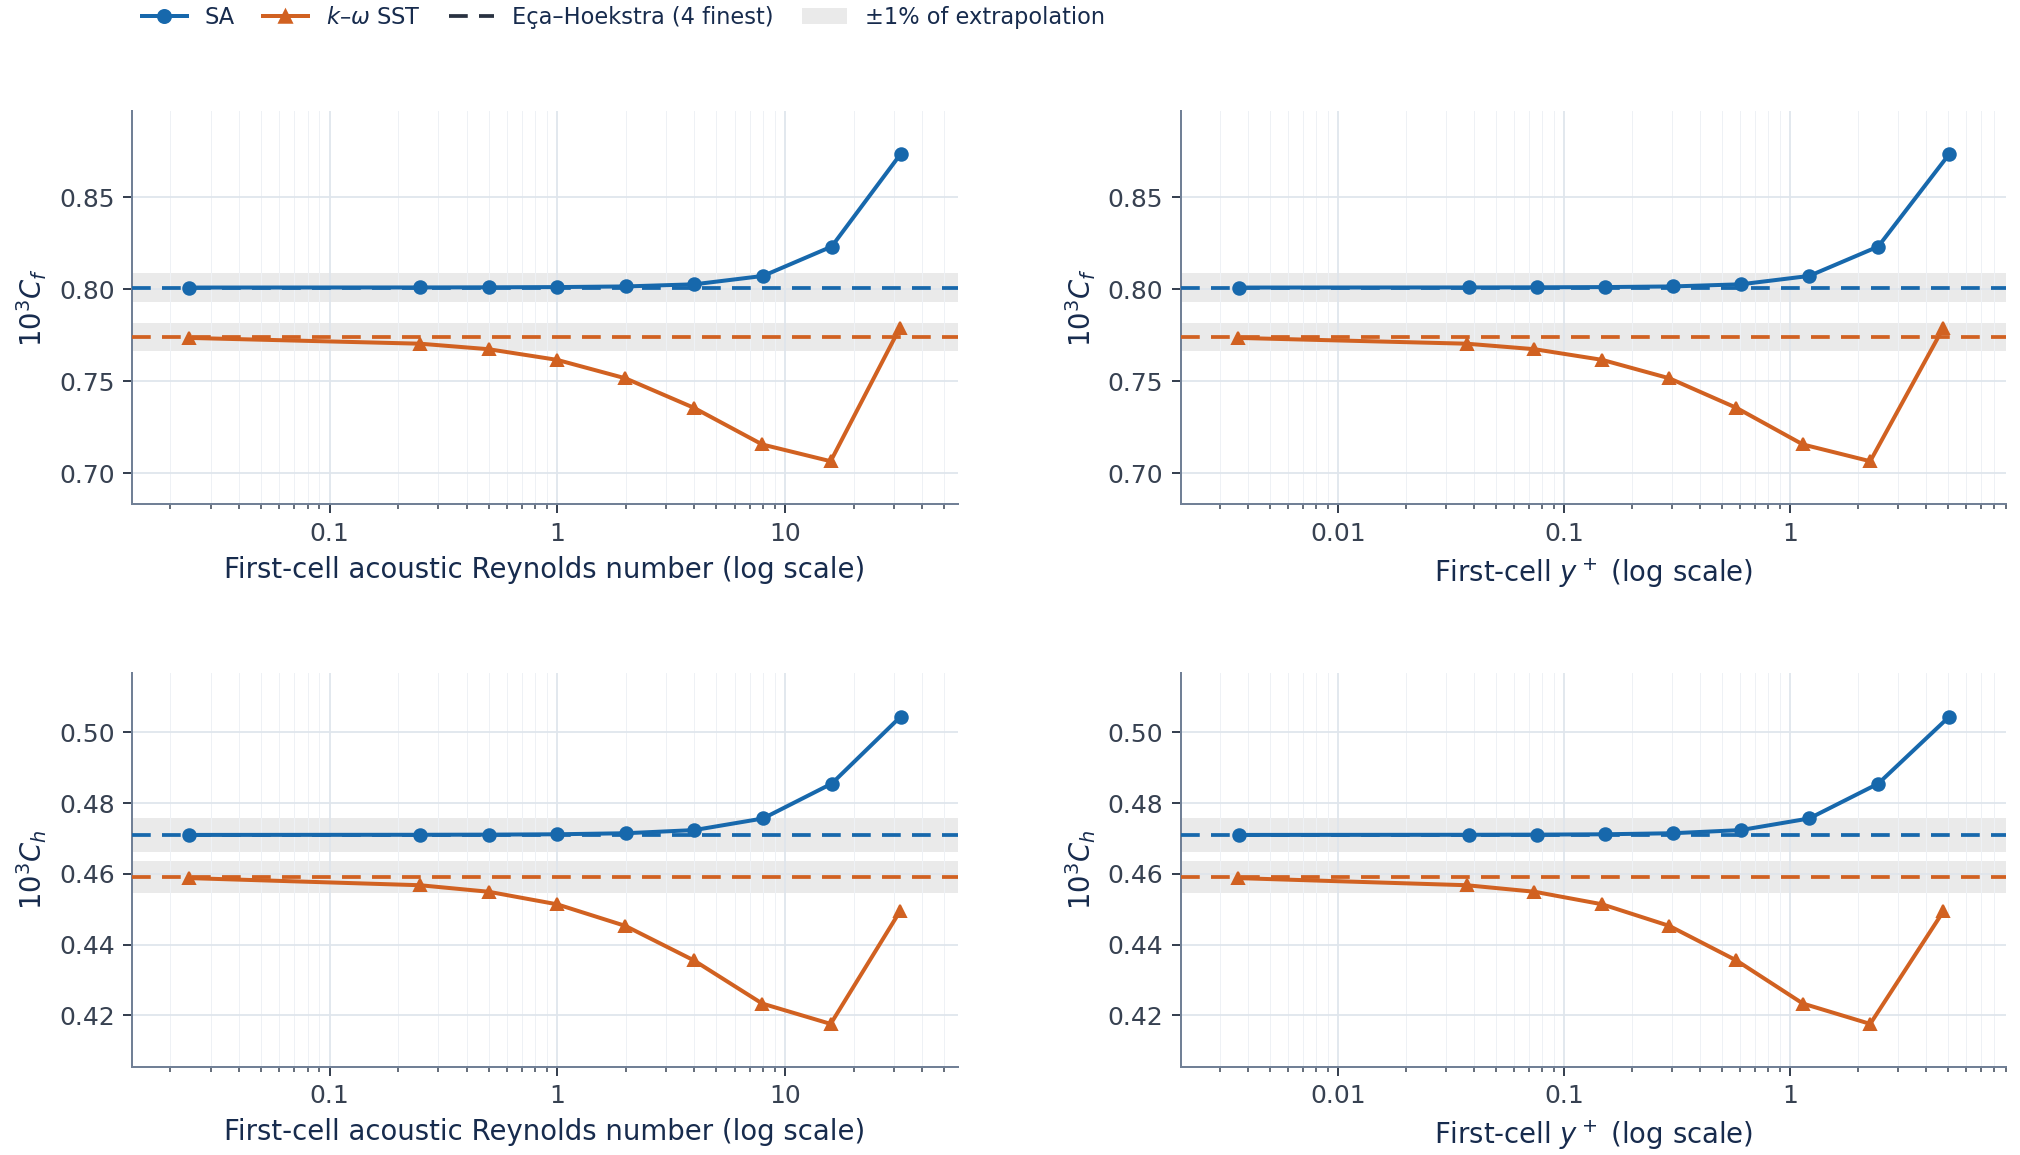
\includegraphics[width=\linewidth]{06_Eval_Methodology/06_Figures/Appendix/Zhang_M8Tw048_Re_delta2.png}
    \caption[Zhang M8Tw048: wall-normal mesh sensitivity]{Wall-normal mesh sensitivity for Zhang M8Tw048, comparing Spalart--Allmaras and \(k\)--\(\omega\) SST. Skin-friction coefficient \(C_f\) (top) and Stanton number \(C_h\) (bottom) versus first-cell acoustic Reynolds number (left) and first-cell \(y^+\) (right) at the matched \(Re_{\delta2}\) = 1990 station. Dashed line represents E\c{c}a--Hoekstra extrapolations from the four finest mesh results; shaded bands mark \(\pm1\%\) of each extrapolated value.}
    \label{fig:app:zpg:mesh:M8Tw048}
\end{figure}

\begin{figure}[!htbp]
    \centering
    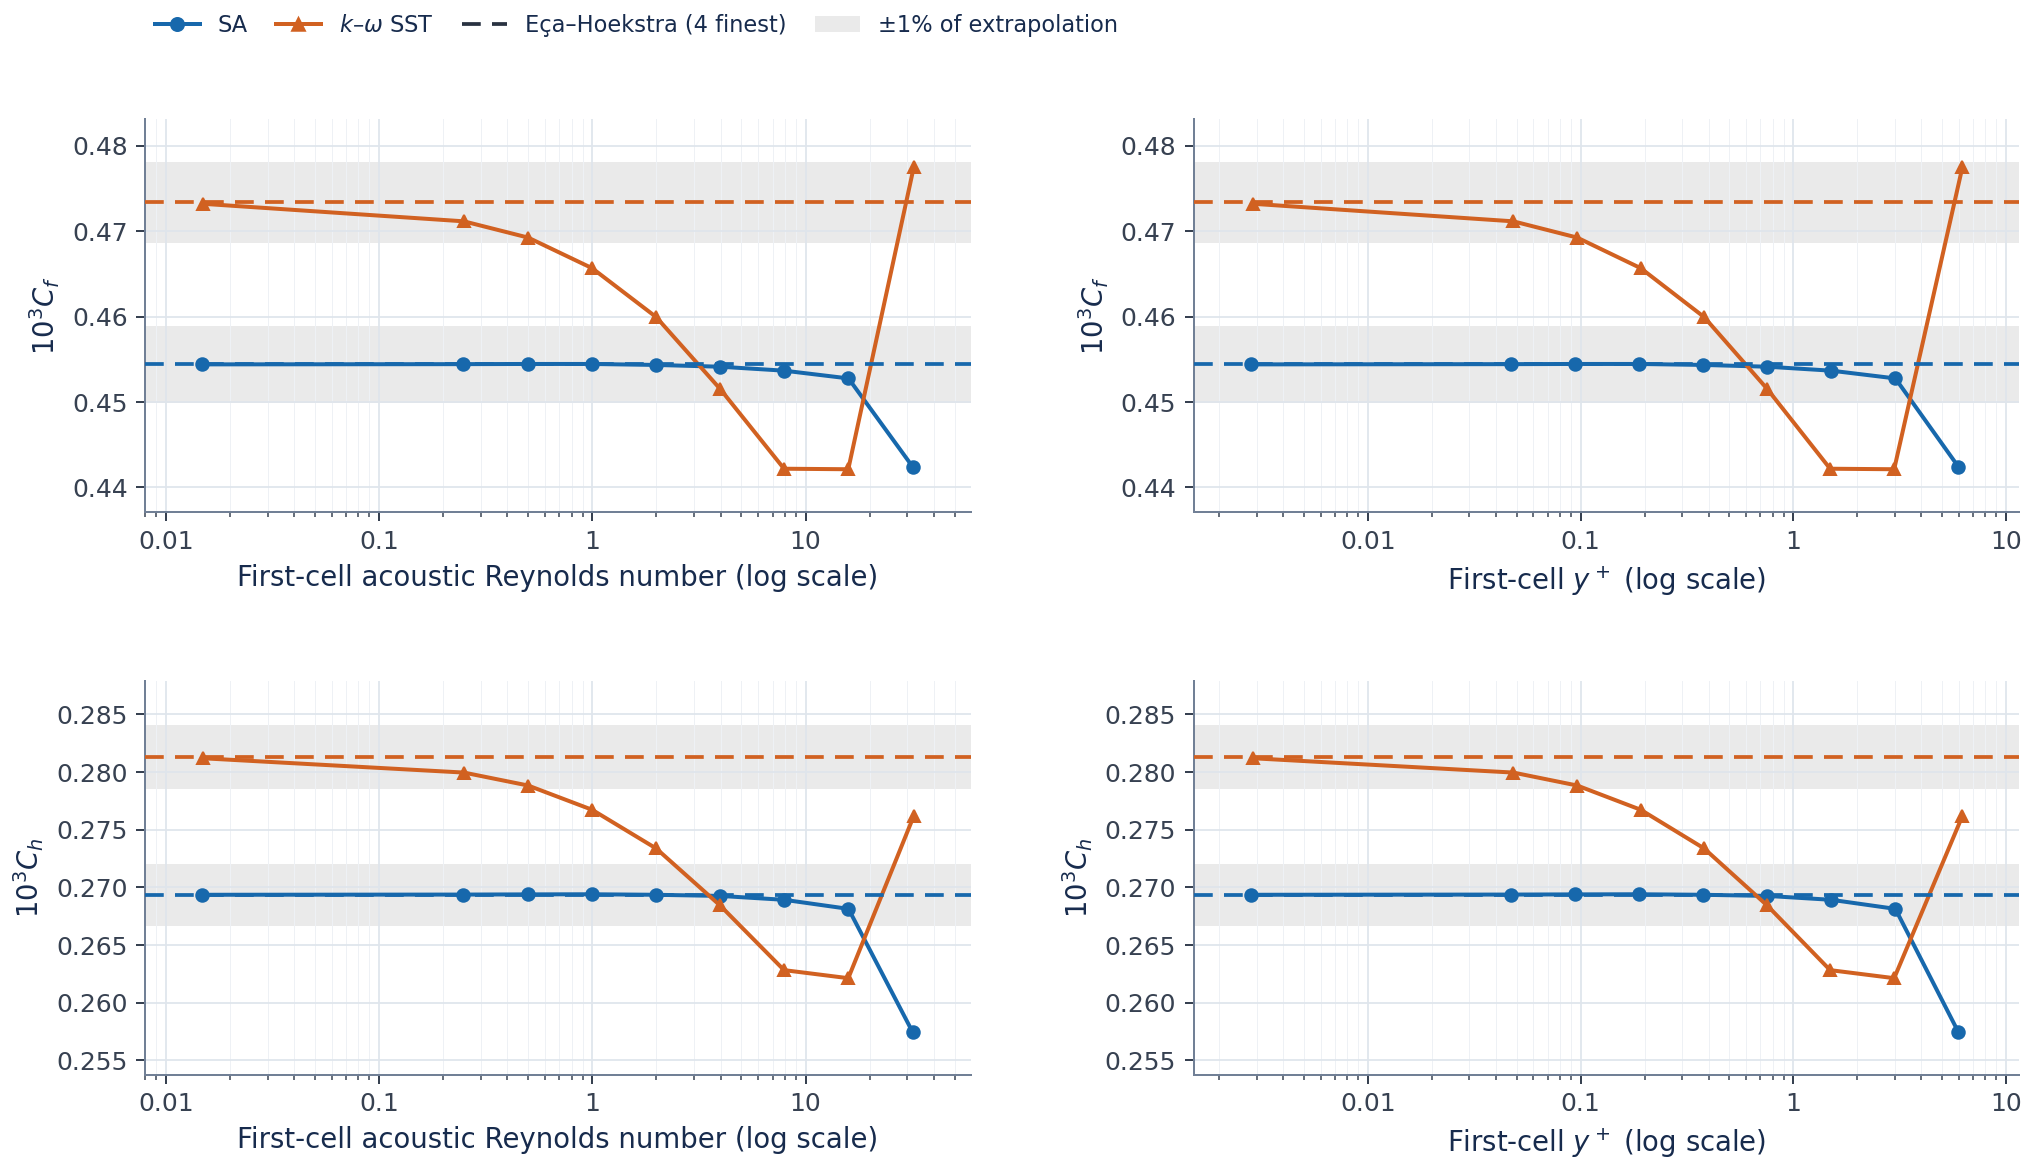
\includegraphics[width=\linewidth]{06_Eval_Methodology/06_Figures/Appendix/Zhang_M14Tw018_Re_delta2.png}
    \caption[Zhang M14Tw018: wall-normal mesh sensitivity]{Wall-normal mesh sensitivity for Zhang M14Tw018, comparing Spalart--Allmaras and \(k\)--\(\omega\) SST. Skin-friction coefficient \(C_f\) (top) and Stanton number \(C_h\) (bottom) versus first-cell acoustic Reynolds number (left) and first-cell \(y^+\) (right) at the matched \(Re_{\delta2}\) = 2354 station. Dashed line represents E\c{c}a--Hoekstra extrapolations from the four finest mesh results; shaded bands mark \(\pm1\%\) of each extrapolated value.}
    \label{fig:app:zpg:mesh:M14Tw018}
\end{figure}

\clearpage
\section{Huang case at stations BL1--BL3}

\begin{figure}[!htbp]
    \centering
    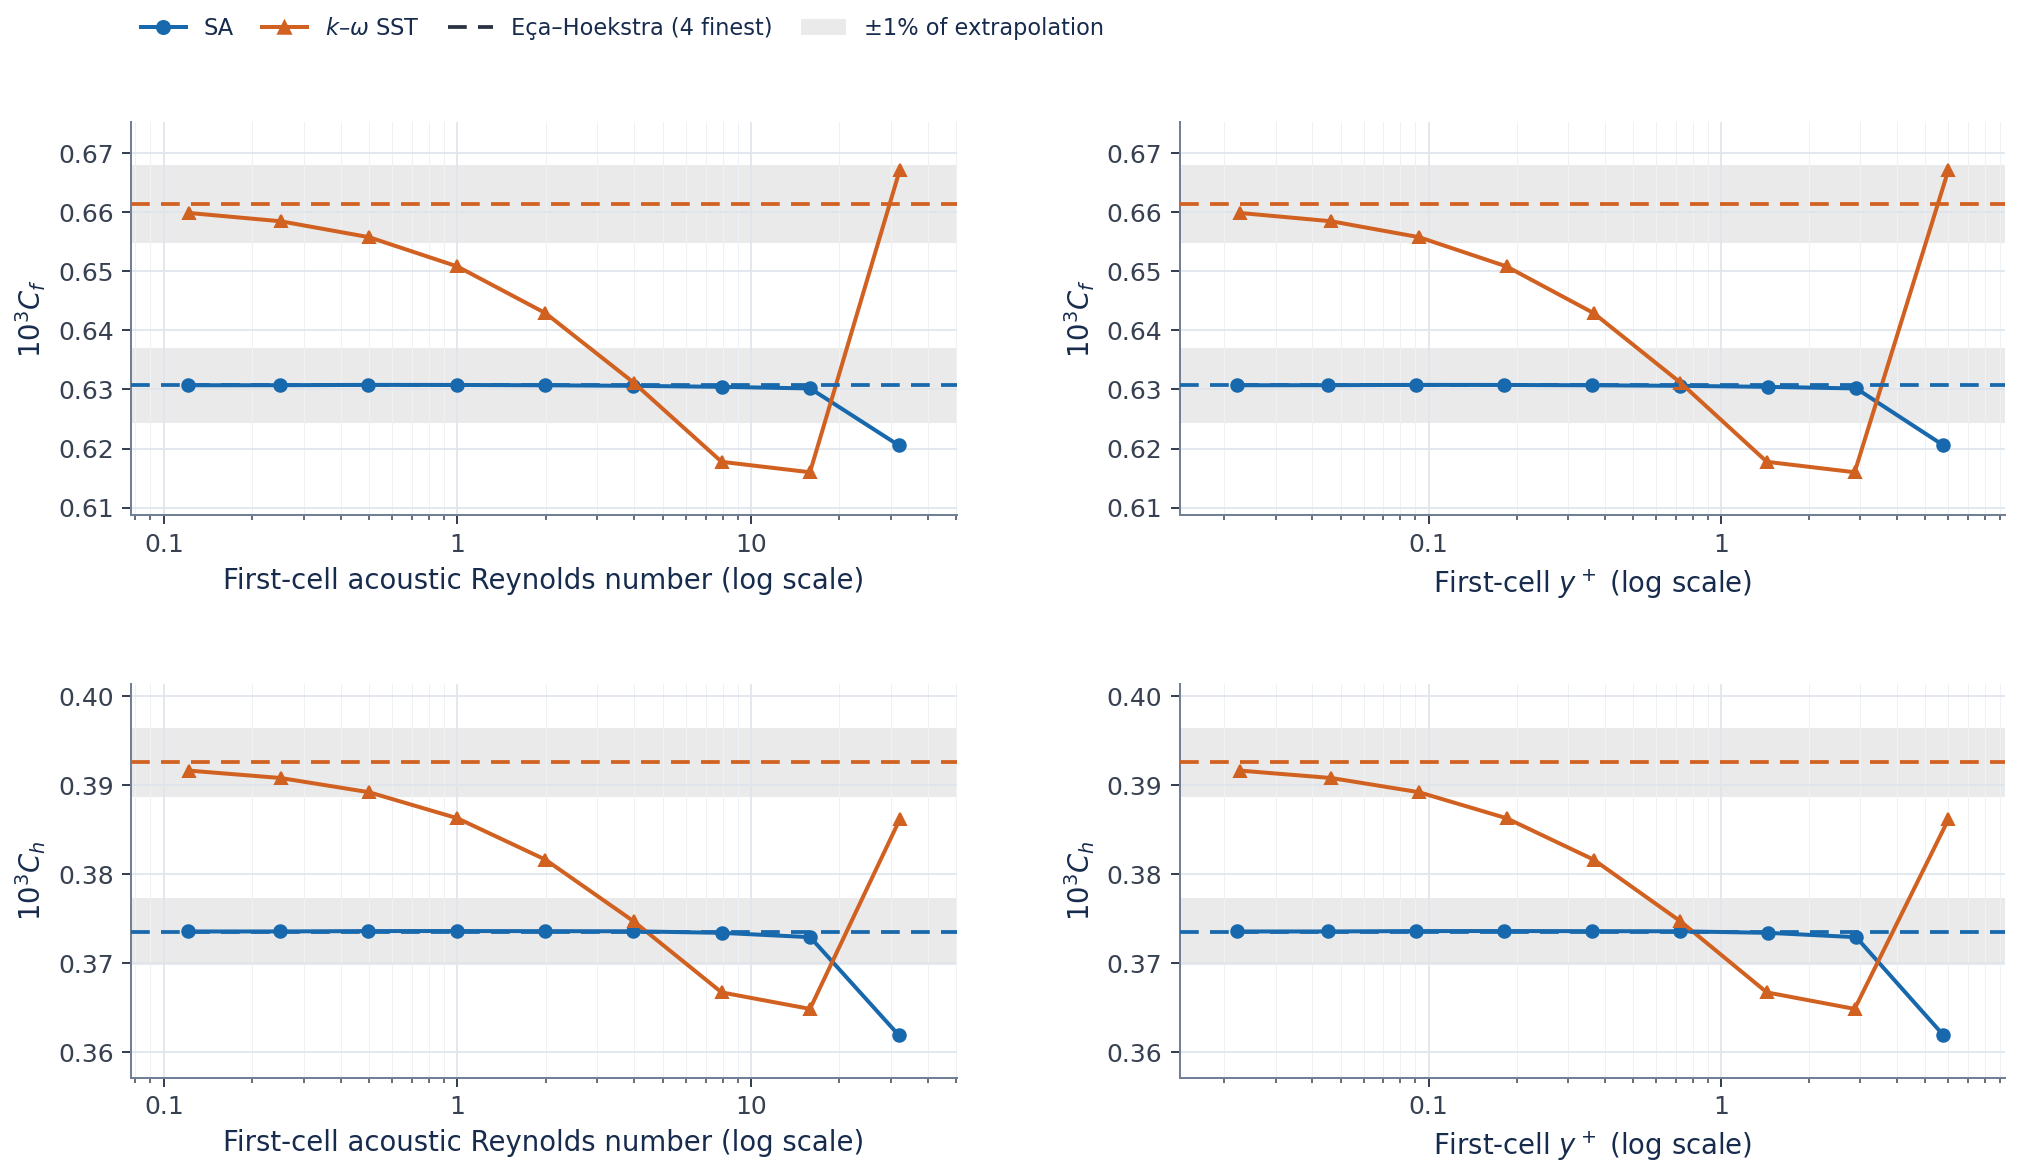
\includegraphics[width=\linewidth]{06_Eval_Methodology/06_Figures/Appendix/Huang_M11Tw20_BL1.png}
    \caption[Huang M11Tw020 at station BL1: wall-normal mesh sensitivity]{Wall-normal mesh sensitivity for Huang M11Tw020 at station BL1, comparing Spalart--Allmaras and \(k\)--\(\omega\) SST. Skin-friction coefficient \(C_f\) (top) and Stanton number \(C_h\) (bottom) versus first-cell acoustic Reynolds number (left) and first-cell \(y^+\) (right) at the matched \(Re_{\delta2}\) = 2204 station. Dashed line represents E\c{c}a--Hoekstra extrapolations from the four finest mesh results; shaded bands mark \(\pm1\%\) of each extrapolated value.}
    \label{fig:app:zpg:mesh:Huang-BL1}
\end{figure}

\begin{figure}[!htbp]
    \centering
    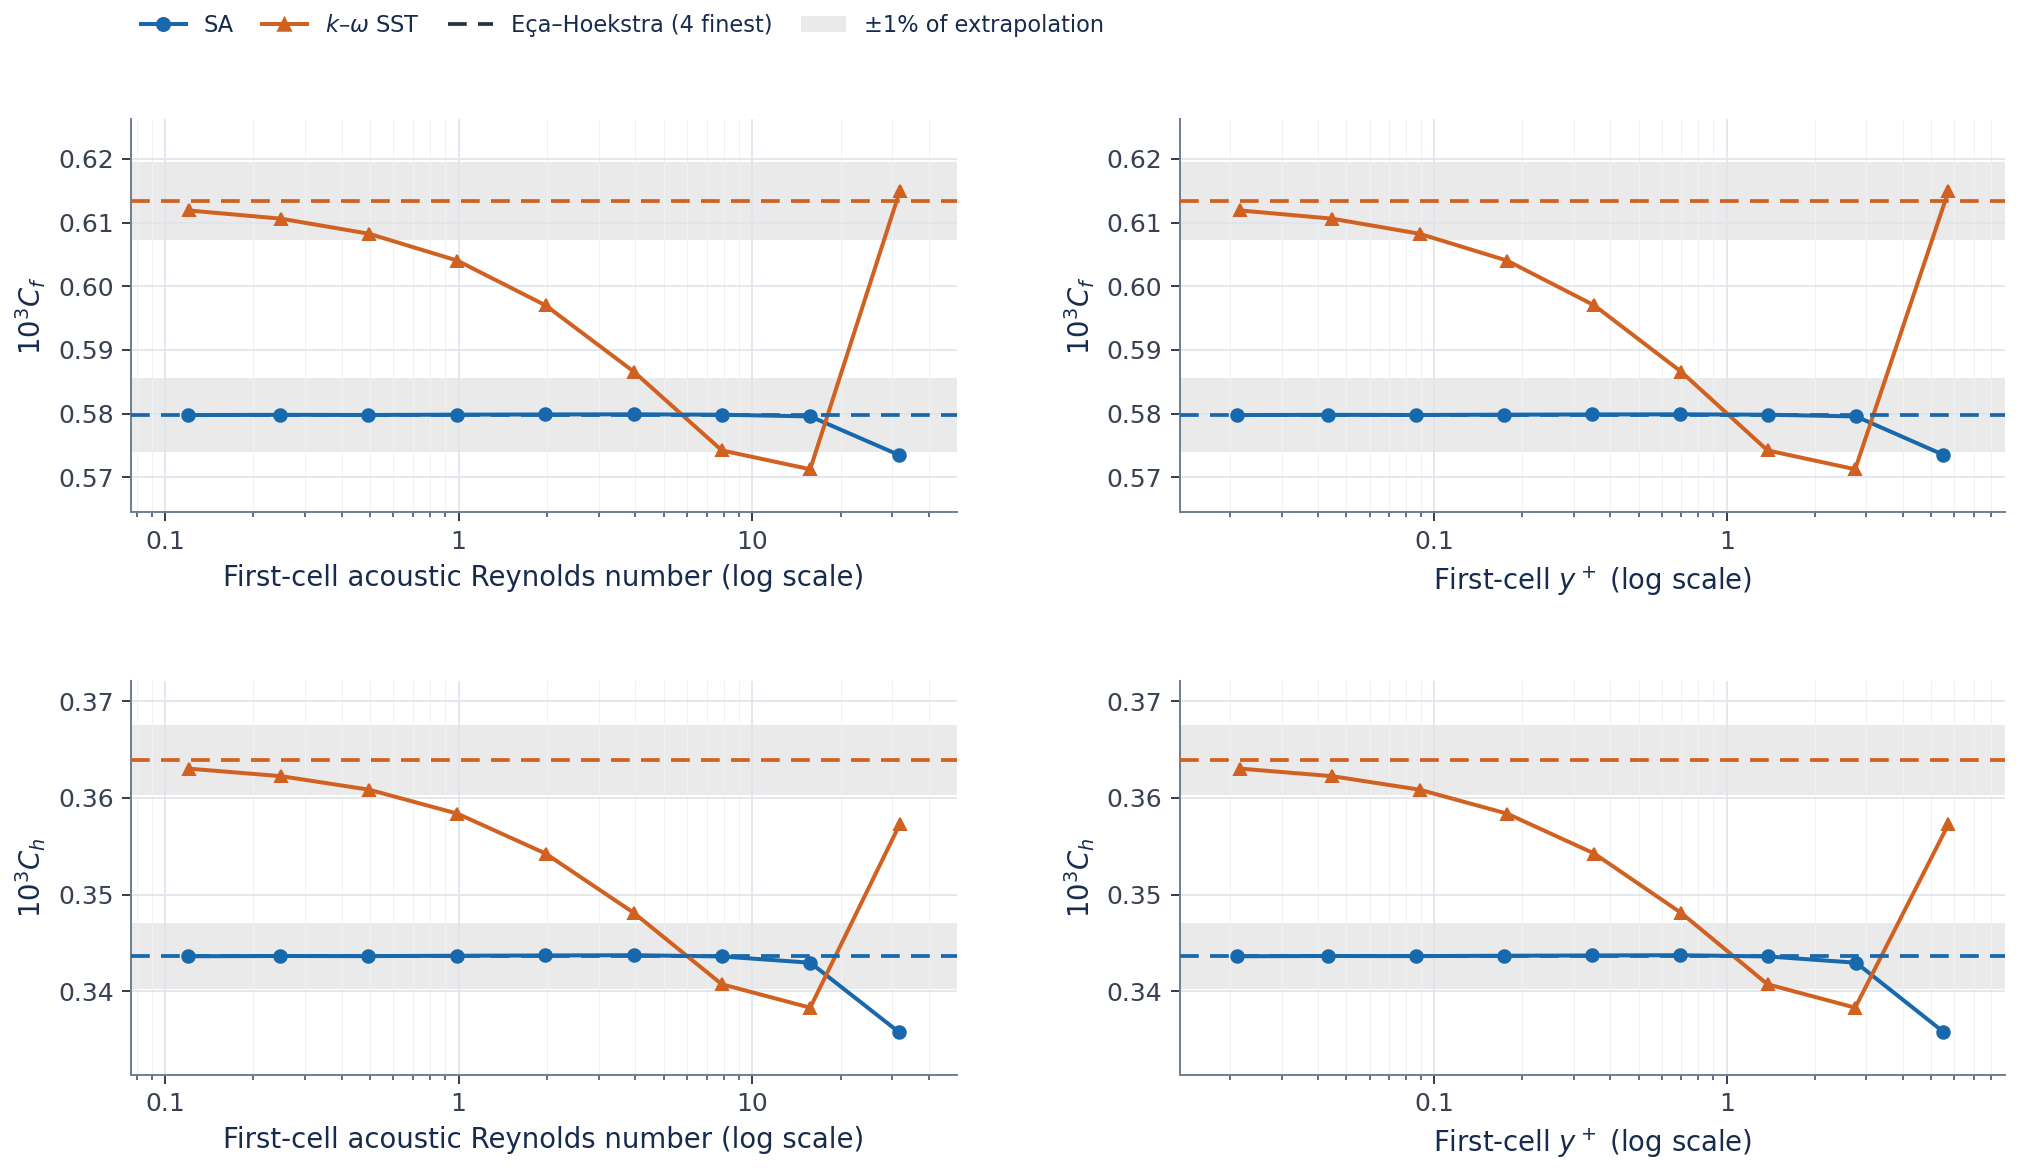
\includegraphics[width=\linewidth]{06_Eval_Methodology/06_Figures/Appendix/Huang_M11Tw20_BL2.png}
    \caption[Huang M11Tw020 at station BL2: wall-normal mesh sensitivity]{Wall-normal mesh sensitivity for Huang M11Tw020 at station BL2, comparing Spalart--Allmaras and \(k\)--\(\omega\) SST. Skin-friction coefficient \(C_f\) (top) and Stanton number \(C_h\) (bottom) versus first-cell acoustic Reynolds number (left) and first-cell \(y^+\) (right) at the matched \(Re_{\delta2}\) = 3419 station. Dashed line represents E\c{c}a--Hoekstra extrapolations from the four finest mesh results; shaded bands mark \(\pm1\%\) of each extrapolated value.}
    \label{fig:app:zpg:mesh:Huang-BL2}
\end{figure}

\begin{figure}[!htbp]
    \centering
    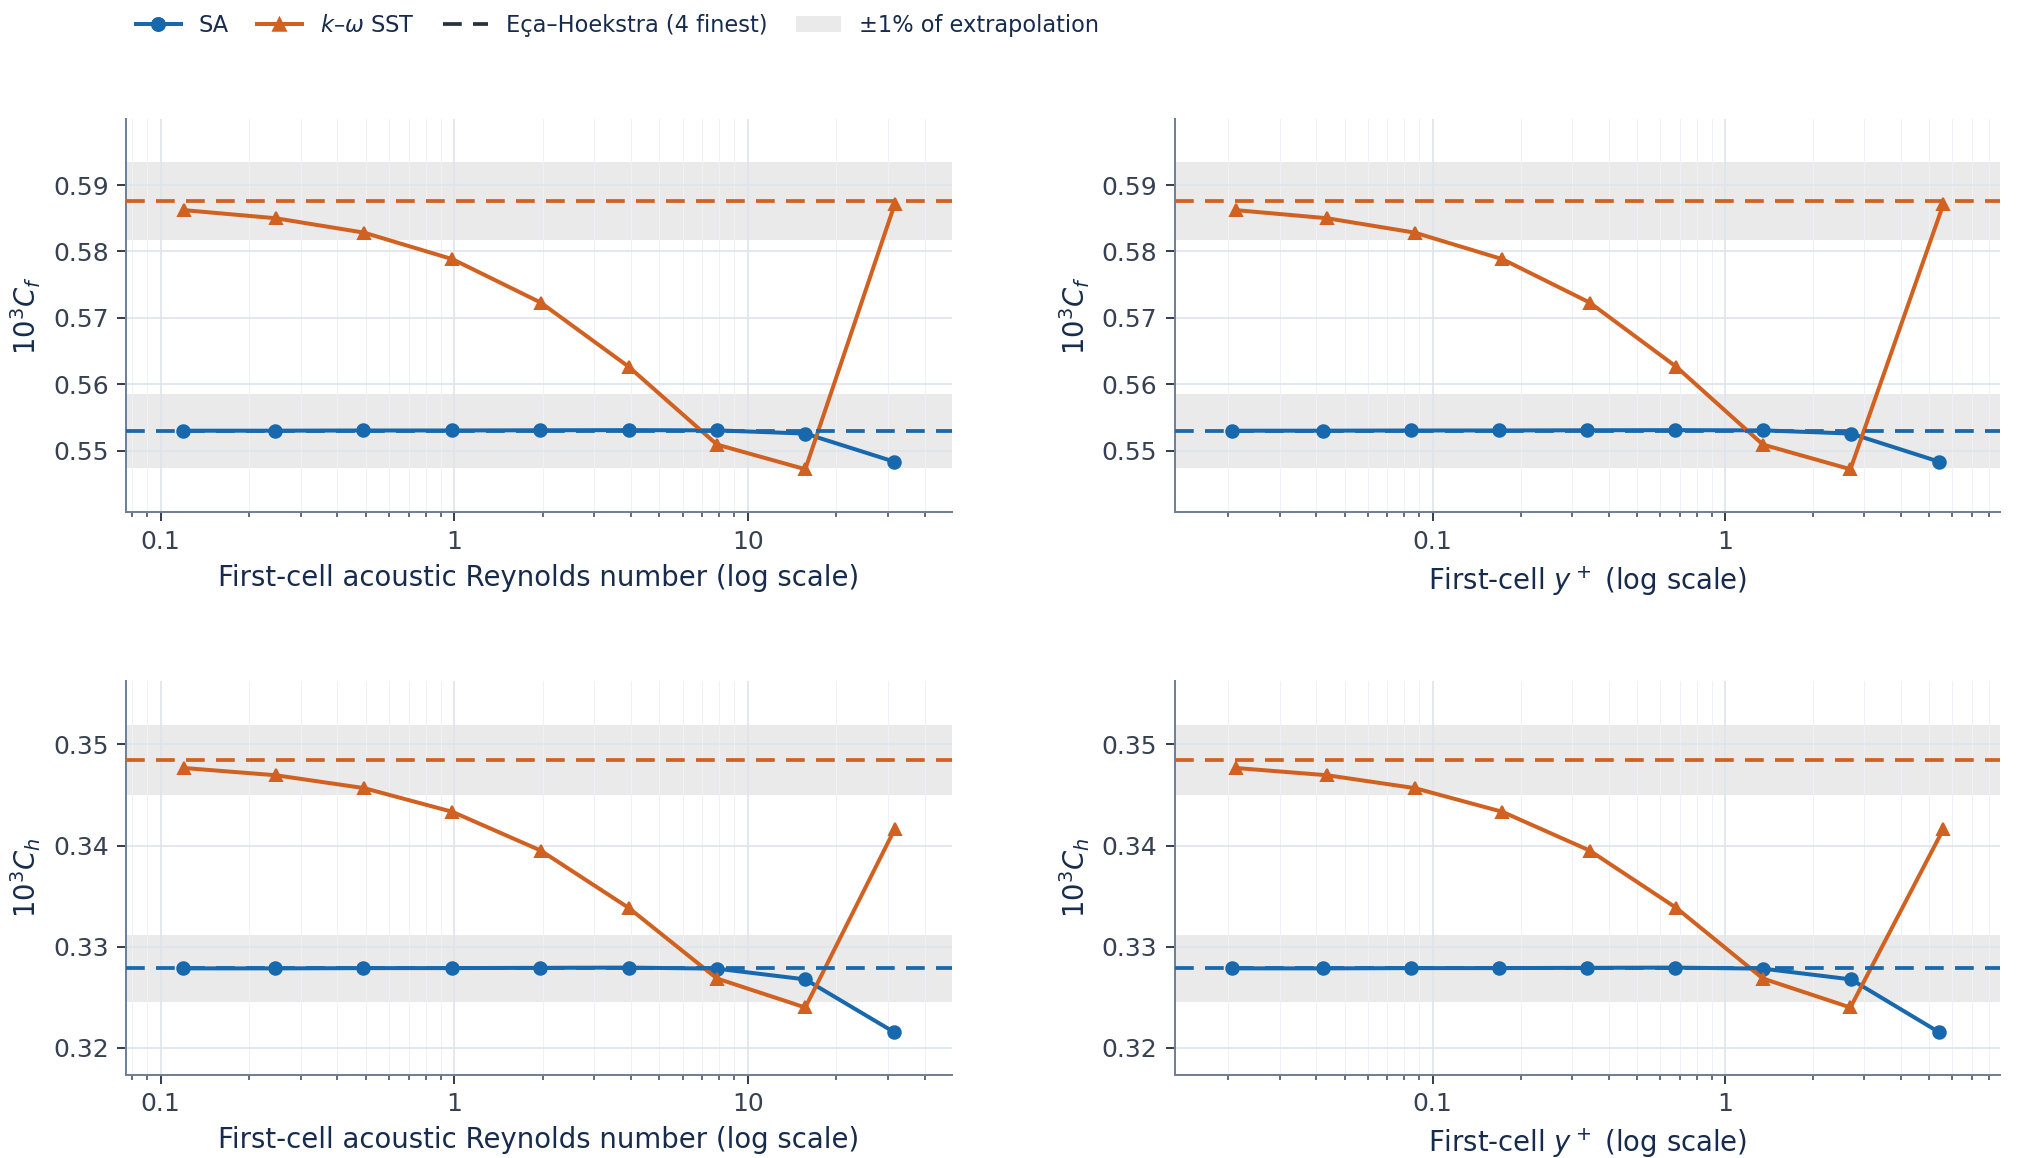
\includegraphics[width=\linewidth]{06_Eval_Methodology/06_Figures/Appendix/Huang_M11Tw20_BL3.png}
    \caption[Huang M11Tw020 at station BL3: wall-normal mesh sensitivity]{Wall-normal mesh sensitivity for Huang M11Tw020 at station BL3, comparing Spalart--Allmaras and \(k\)--\(\omega\) SST. Skin-friction coefficient \(C_f\) (top) and Stanton number \(C_h\) (bottom) versus first-cell acoustic Reynolds number (left) and first-cell \(y^+\) (right) at the matched \(Re_{\delta2}\) = 4390 station. Dashed line represents E\c{c}a--Hoekstra extrapolations from the four finest mesh results; shaded bands mark \(\pm1\%\) of each extrapolated value.}
    \label{fig:app:zpg:mesh:Huang-BL3}
\end{figure}
\chapter{Additional wall-resolved boundary layer profiles}
\label{app:zpg:wr-profiles}

This appendix supplements Section~\ref{sec:comparative:zpg:wall-resolved-baselines}
with the ten case comparisons accompanying the M6Tw025 and LowH\_M3 profiles
shown in the main text. The plots compare wall-resolved Spalart--Allmaras
and \(k\)--\(\omega\) SST predictions at \(Pr_t=0.9\) with the DNS references.
Matching conventions and reference-data limitations are described in
Section~\ref{sec:evaluation:benchmark-cases}.

\section{Martin--Duan Part 2}

The digitized profiles use the inferred temperature normalization described
in Section~\ref{sec:evaluation:benchmark-cases}. The published \(Re_{\delta2}\)
values remain nominal matching targets, subject to the inconsistency
discussed in Appendix~\ref{app:duan:reynolds}.

\begin{figure}[!htbp]
    \centering
    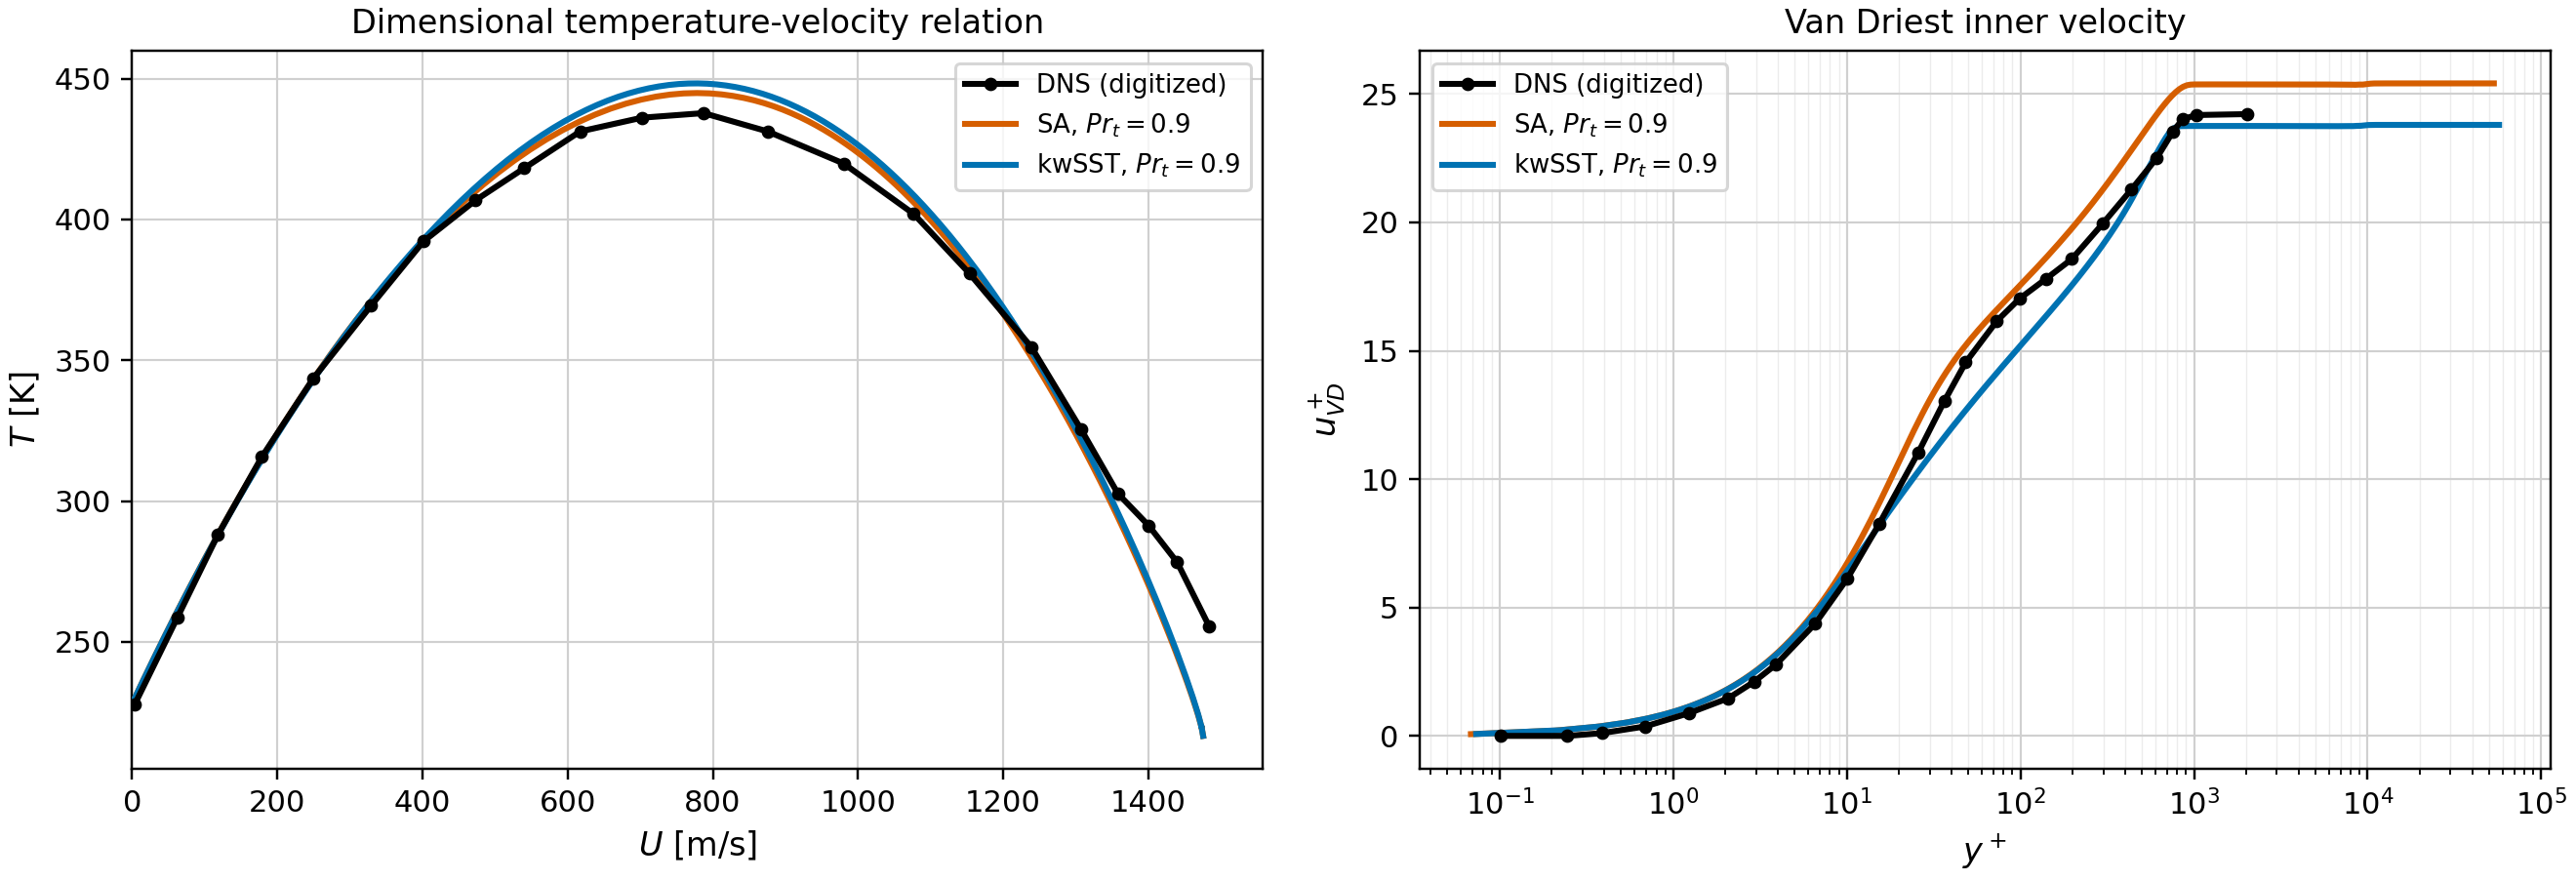
\includegraphics[width=\linewidth]{07_Error_Isolation_Results/Figures/Appendix/WR_BL_profile/Part2_M5T1_profiles.png}
    \caption[M5T1: wall-resolved boundary layer profiles]{Wall-resolved Spalart--Allmaras and \(k\)--\(\omega\) SST profiles for M5T1 at \(Pr_t=0.9\), compared with digitized Martin--Duan Part~2 DNS data~\cite{duan2010direct_part2}. Left: dimensional temperature--velocity relation \(T(U)\). Right: van Driest--transformed velocity \(U_{\mathrm{VD}}^+\) versus wall distance \(y^+\) at the matched \(Re_{\delta2}\) = 1538.4 station.}
    \label{fig:app:zpg:profiles:M5T1}
\end{figure}

\begin{figure}[!htbp]
    \centering
    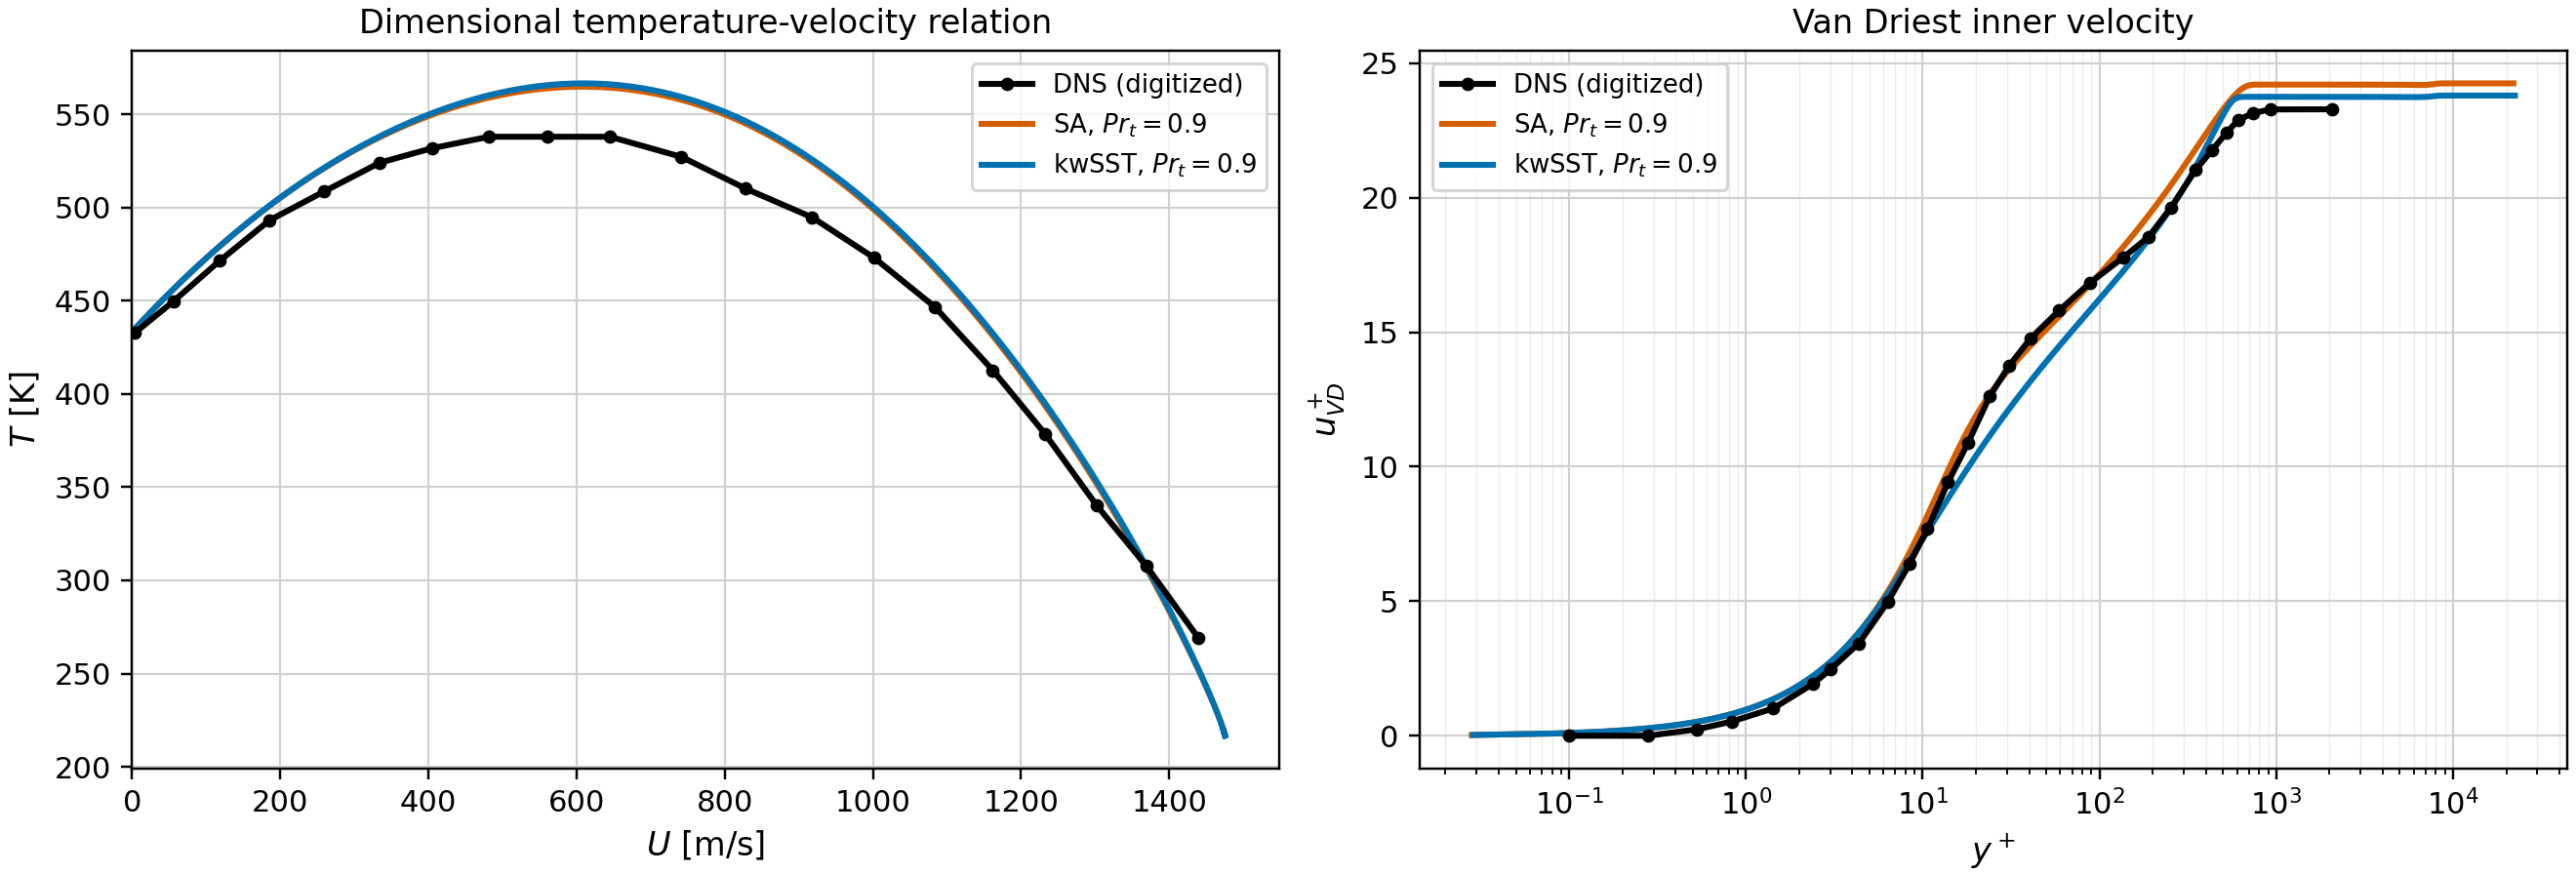
\includegraphics[width=\linewidth]{07_Error_Isolation_Results/Figures/Appendix/WR_BL_profile/Part2_M5T2_profiles.png}
    \caption[M5T2: wall-resolved boundary layer profiles]{Wall-resolved Spalart--Allmaras and \(k\)--\(\omega\) SST profiles for M5T2 at \(Pr_t=0.9\), compared with digitized Martin--Duan Part~2 DNS data~\cite{duan2010direct_part2}. Left: dimensional temperature--velocity relation \(T(U)\). Right: van Driest--transformed velocity \(U_{\mathrm{VD}}^+\) versus wall distance \(y^+\) at the matched \(Re_{\delta2}\) = 1521.5 station.}
    \label{fig:app:zpg:profiles:M5T2}
\end{figure}

\begin{figure}[!htbp]
    \centering
    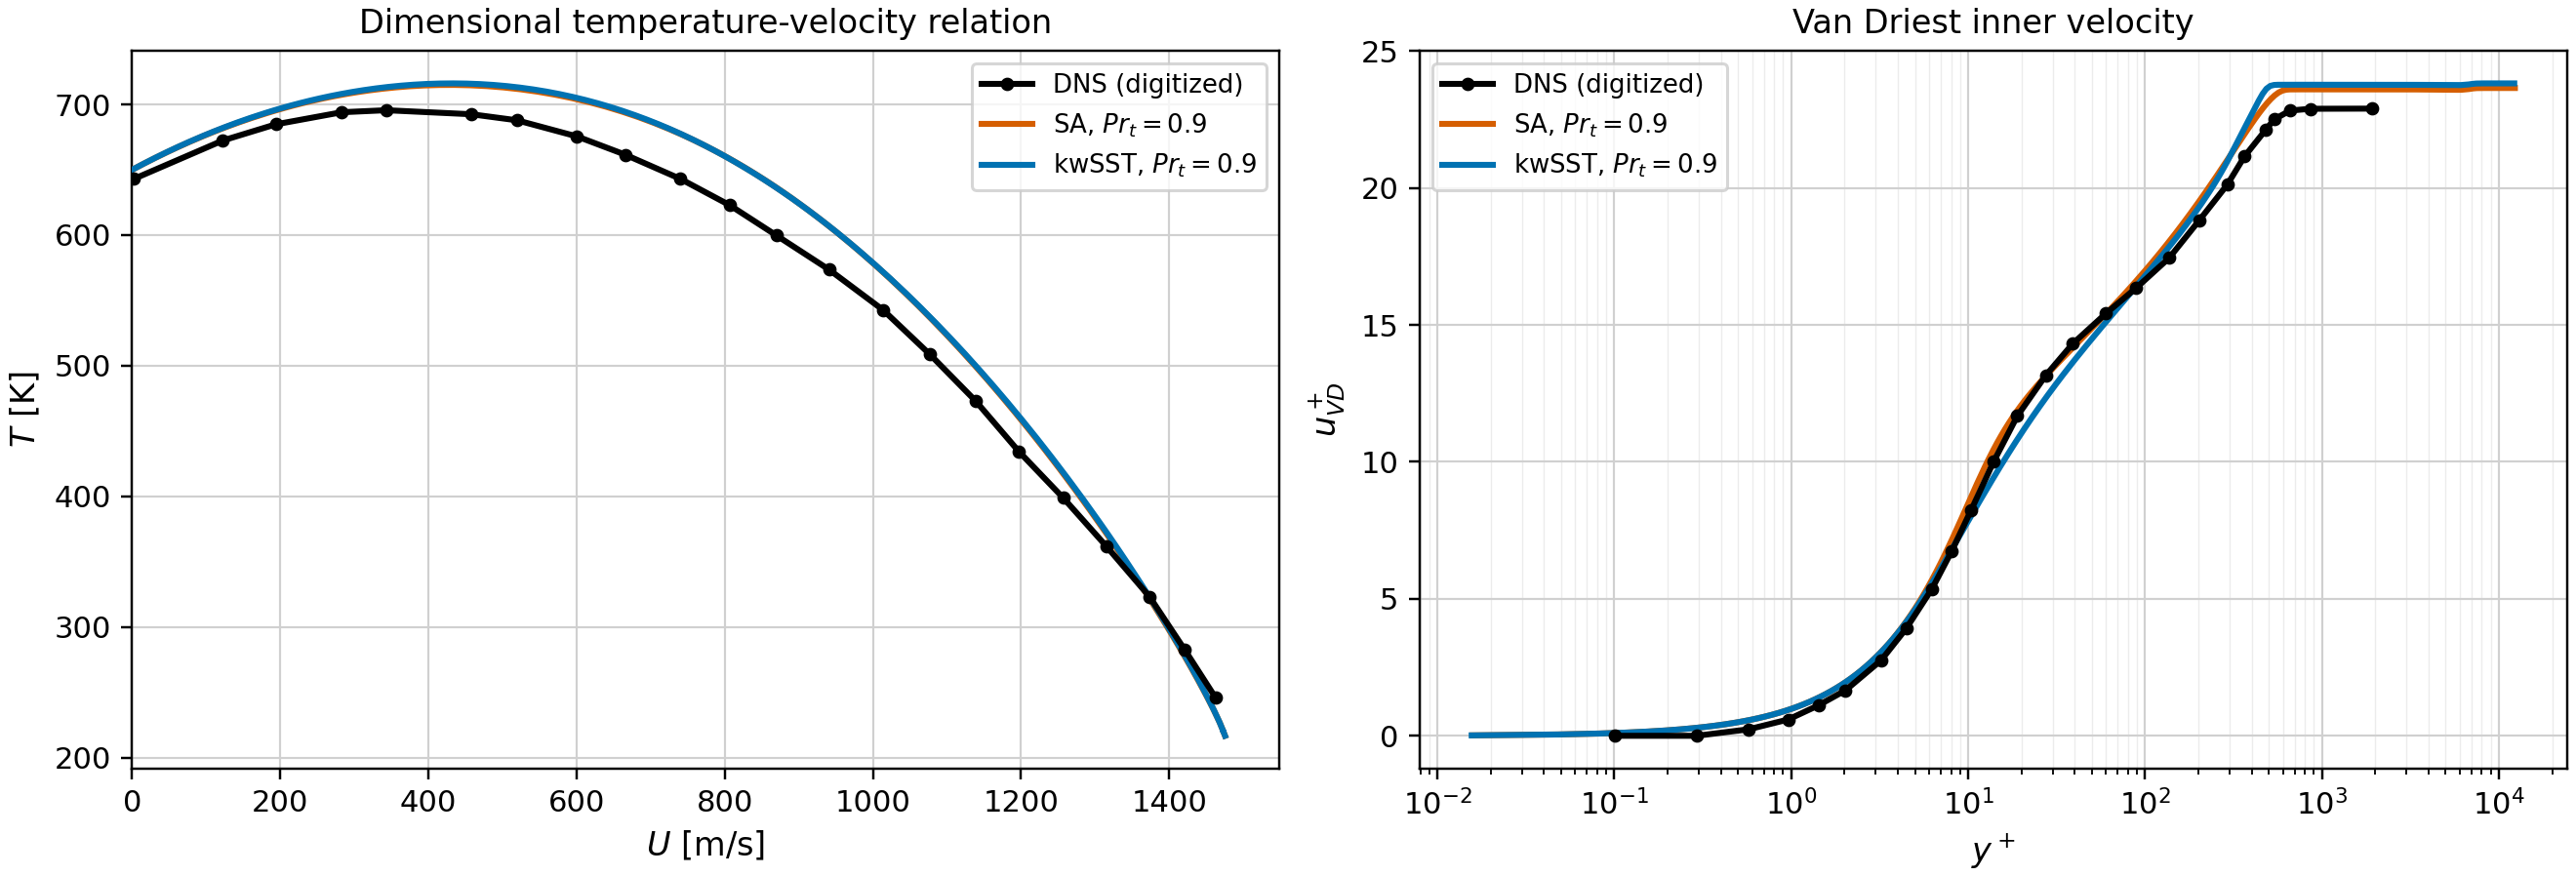
\includegraphics[width=\linewidth]{07_Error_Isolation_Results/Figures/Appendix/WR_BL_profile/Part2_M5T3_profiles.png}
    \caption[M5T3: wall-resolved boundary layer profiles]{Wall-resolved Spalart--Allmaras and \(k\)--\(\omega\) SST profiles for M5T3 at \(Pr_t=0.9\), compared with digitized Martin--Duan Part~2 DNS data~\cite{duan2010direct_part2}. Left: dimensional temperature--velocity relation \(T(U)\). Right: van Driest--transformed velocity \(U_{\mathrm{VD}}^+\) versus wall distance \(y^+\) at the matched \(Re_{\delta2}\) = 1524.7 station.}
    \label{fig:app:zpg:profiles:M5T3}
\end{figure}

\begin{figure}[!htbp]
    \centering
    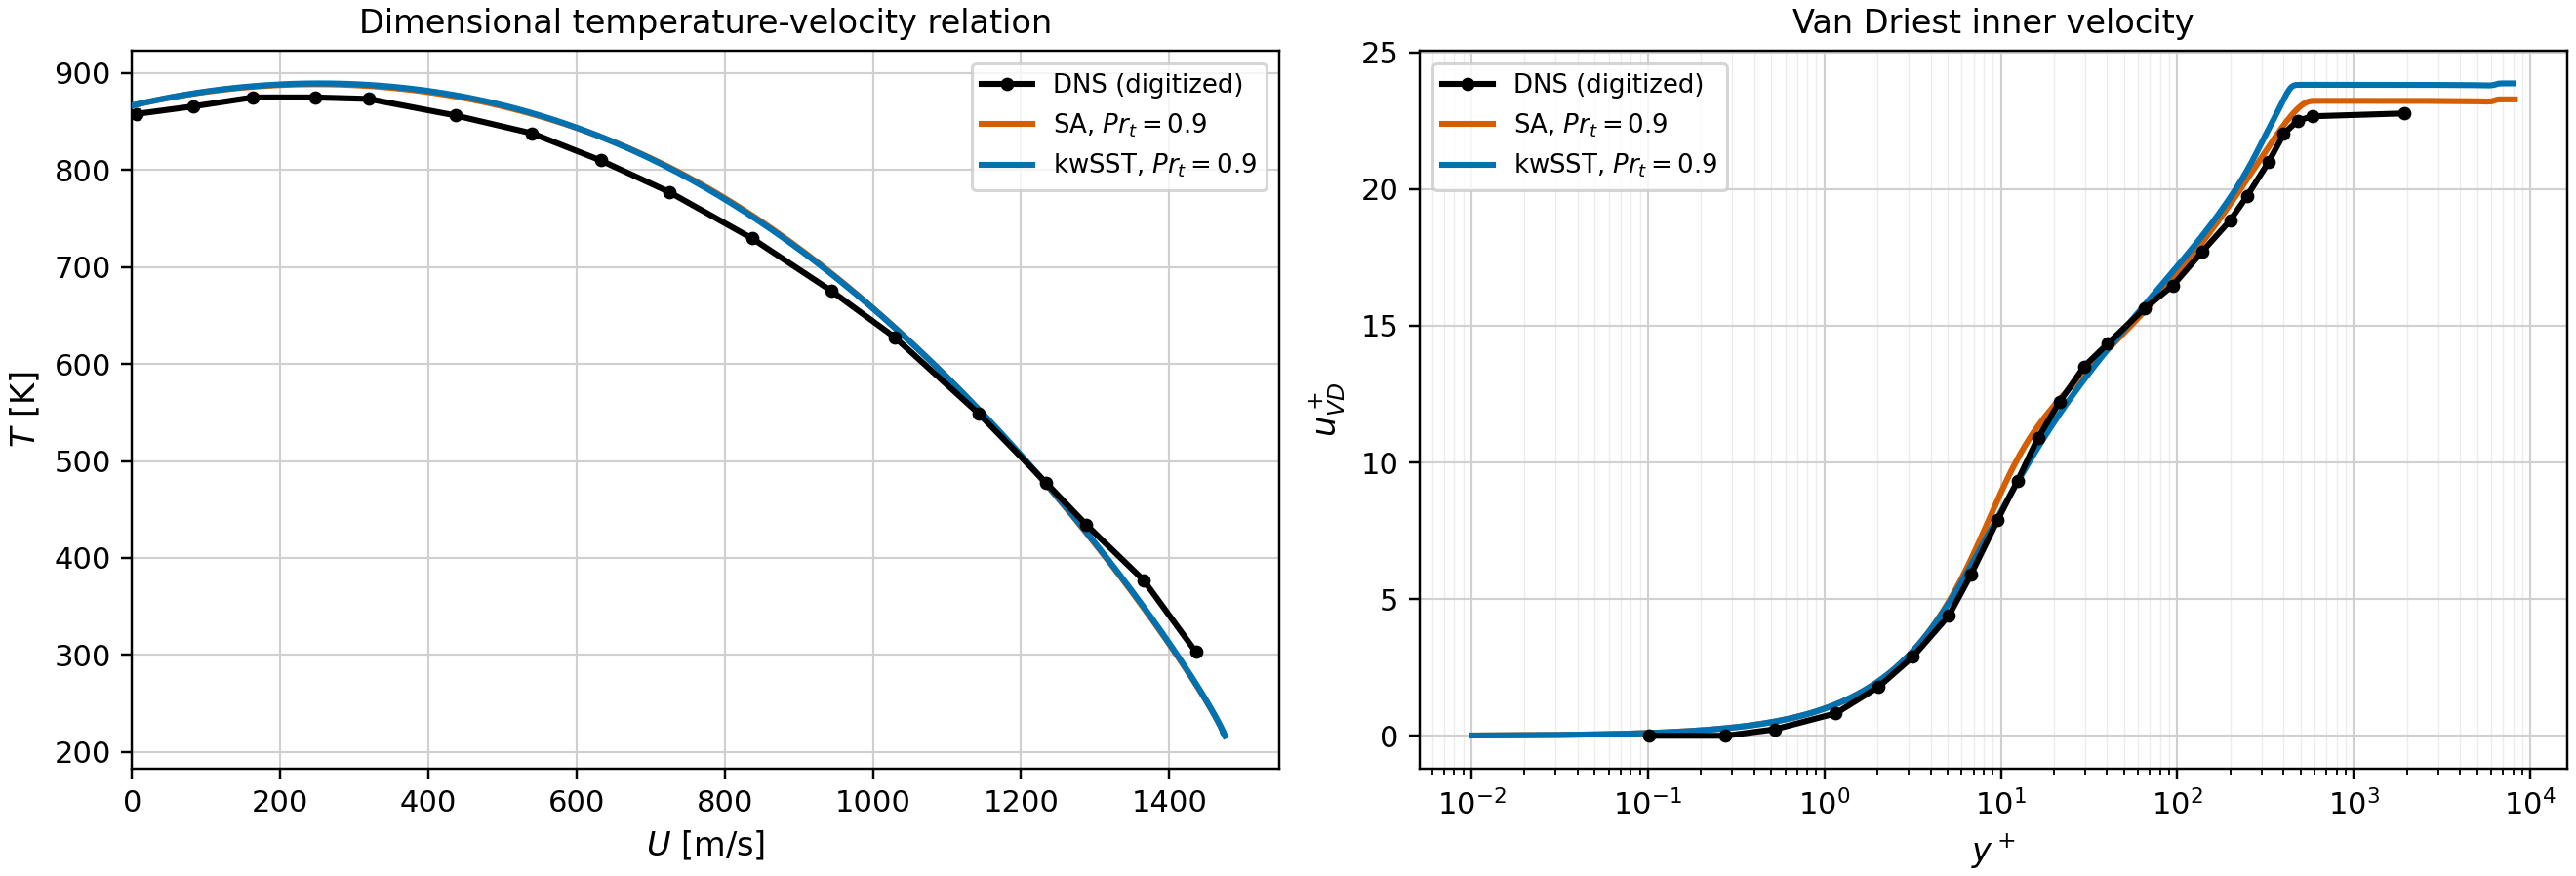
\includegraphics[width=\linewidth]{07_Error_Isolation_Results/Figures/Appendix/WR_BL_profile/Part2_M5T4_profiles.png}
    \caption[M5T4: wall-resolved boundary layer profiles]{Wall-resolved Spalart--Allmaras and \(k\)--\(\omega\) SST profiles for M5T4 at \(Pr_t=0.9\), compared with digitized Martin--Duan Part~2 DNS data~\cite{duan2010direct_part2}. Left: dimensional temperature--velocity relation \(T(U)\). Right: van Driest--transformed velocity \(U_{\mathrm{VD}}^+\) versus wall distance \(y^+\) at the matched \(Re_{\delta2}\) = 1526.4 station.}
    \label{fig:app:zpg:profiles:M5T4}
\end{figure}

\begin{figure}[!htbp]
    \centering
    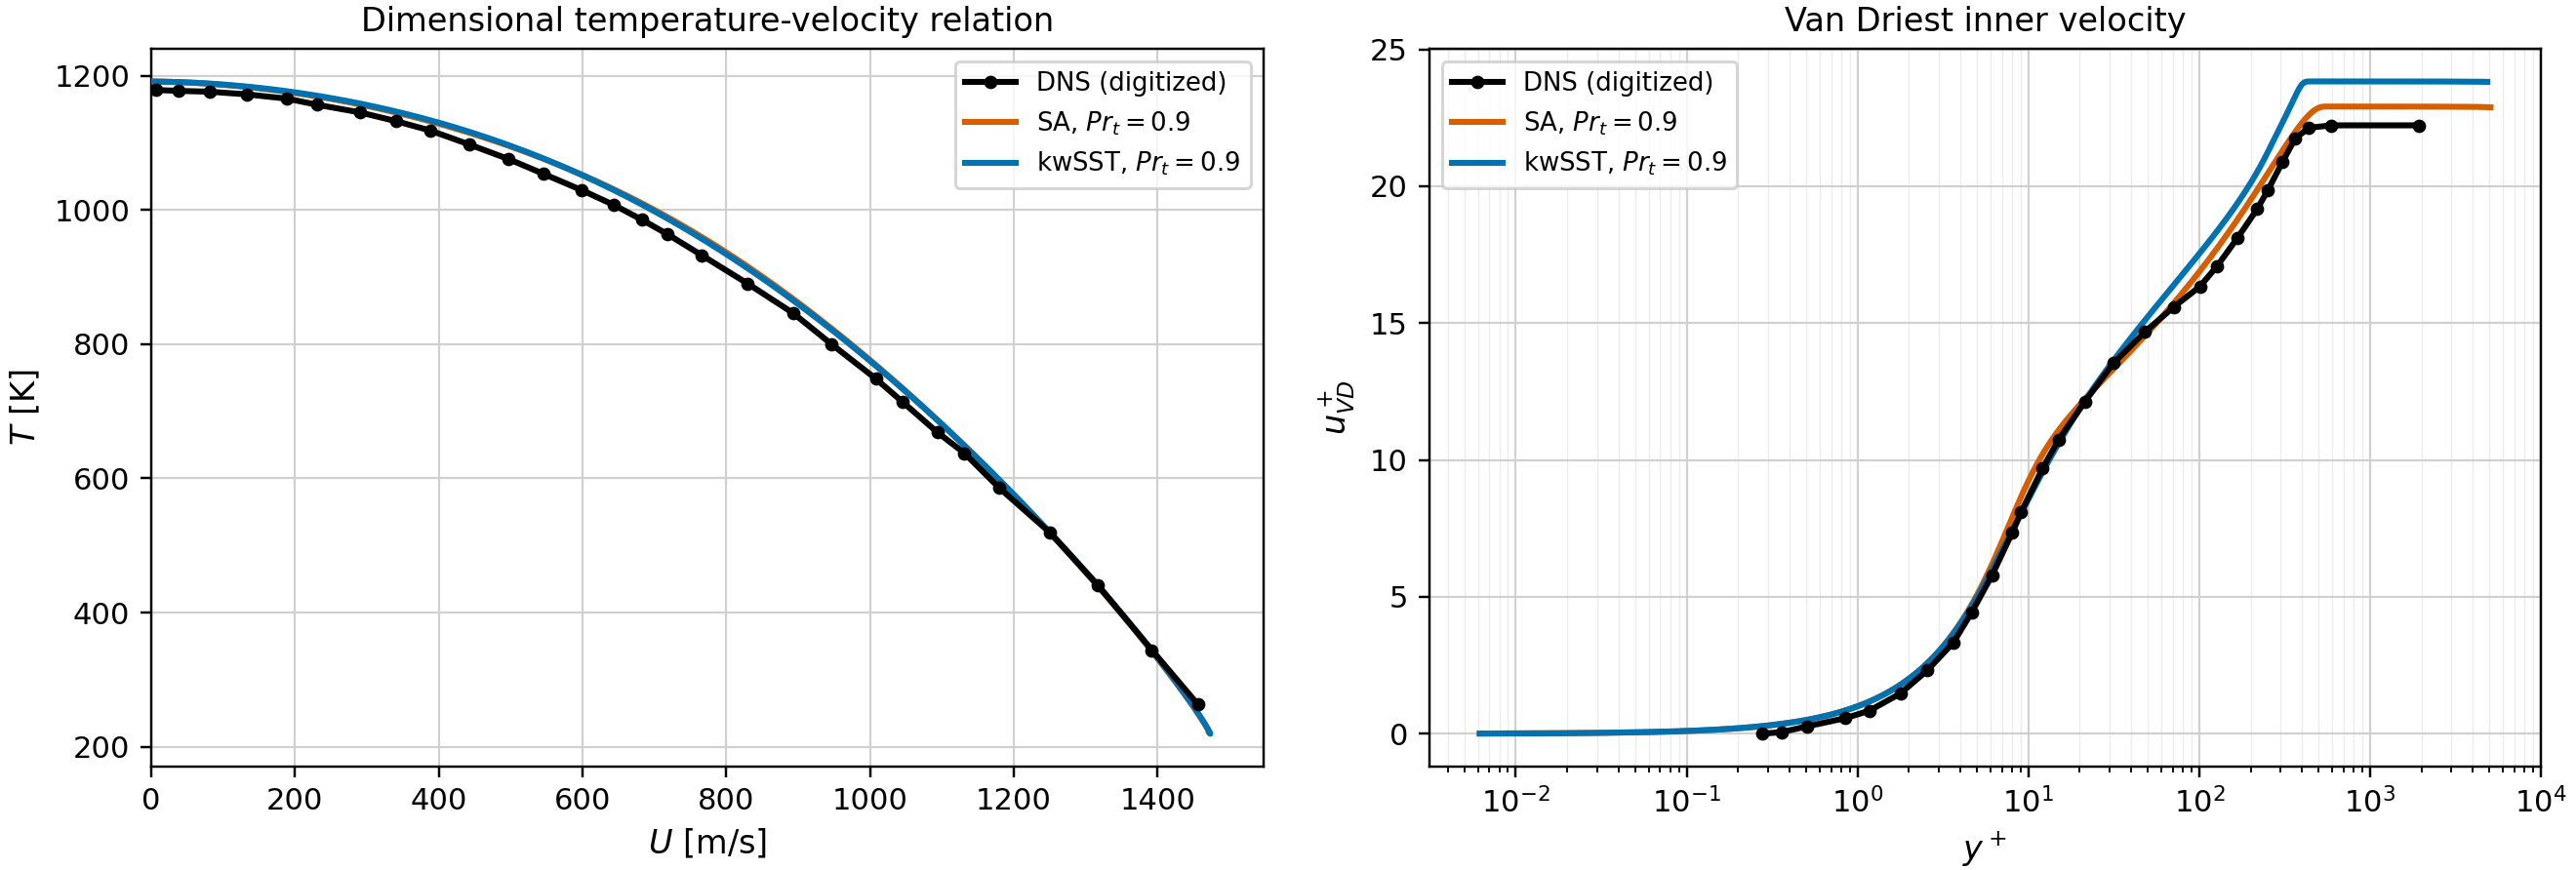
\includegraphics[width=\linewidth]{07_Error_Isolation_Results/Figures/Appendix/WR_BL_profile/Part2_M5T5_profiles.png}
    \caption[M5T5: wall-resolved boundary layer profiles]{Wall-resolved Spalart--Allmaras and \(k\)--\(\omega\) SST profiles for M5T5 at \(Pr_t=0.9\), compared with digitized Martin--Duan Part~2 DNS data~\cite{duan2010direct_part2}. Left: dimensional temperature--velocity relation \(T(U)\). Right: van Driest--transformed velocity \(U_{\mathrm{VD}}^+\) versus wall distance \(y^+\) at the matched \(Re_{\delta2}\) = 1536.8 station.}
    \label{fig:app:zpg:profiles:M5T5}
\end{figure}

\clearpage
\section{Zhang cases}

The following comparisons use the digital DNS profiles of
Zhang et al.~\cite{zhang2018direct}. The M6Tw076 profiles are retained as
qualitative comparisons; the wall-temperature inconsistency and limitations
on quantitative heat-flux assessment remain those described in
Section~\ref{sec:evaluation:benchmark-cases}.

\begin{figure}[!htbp]
    \centering
    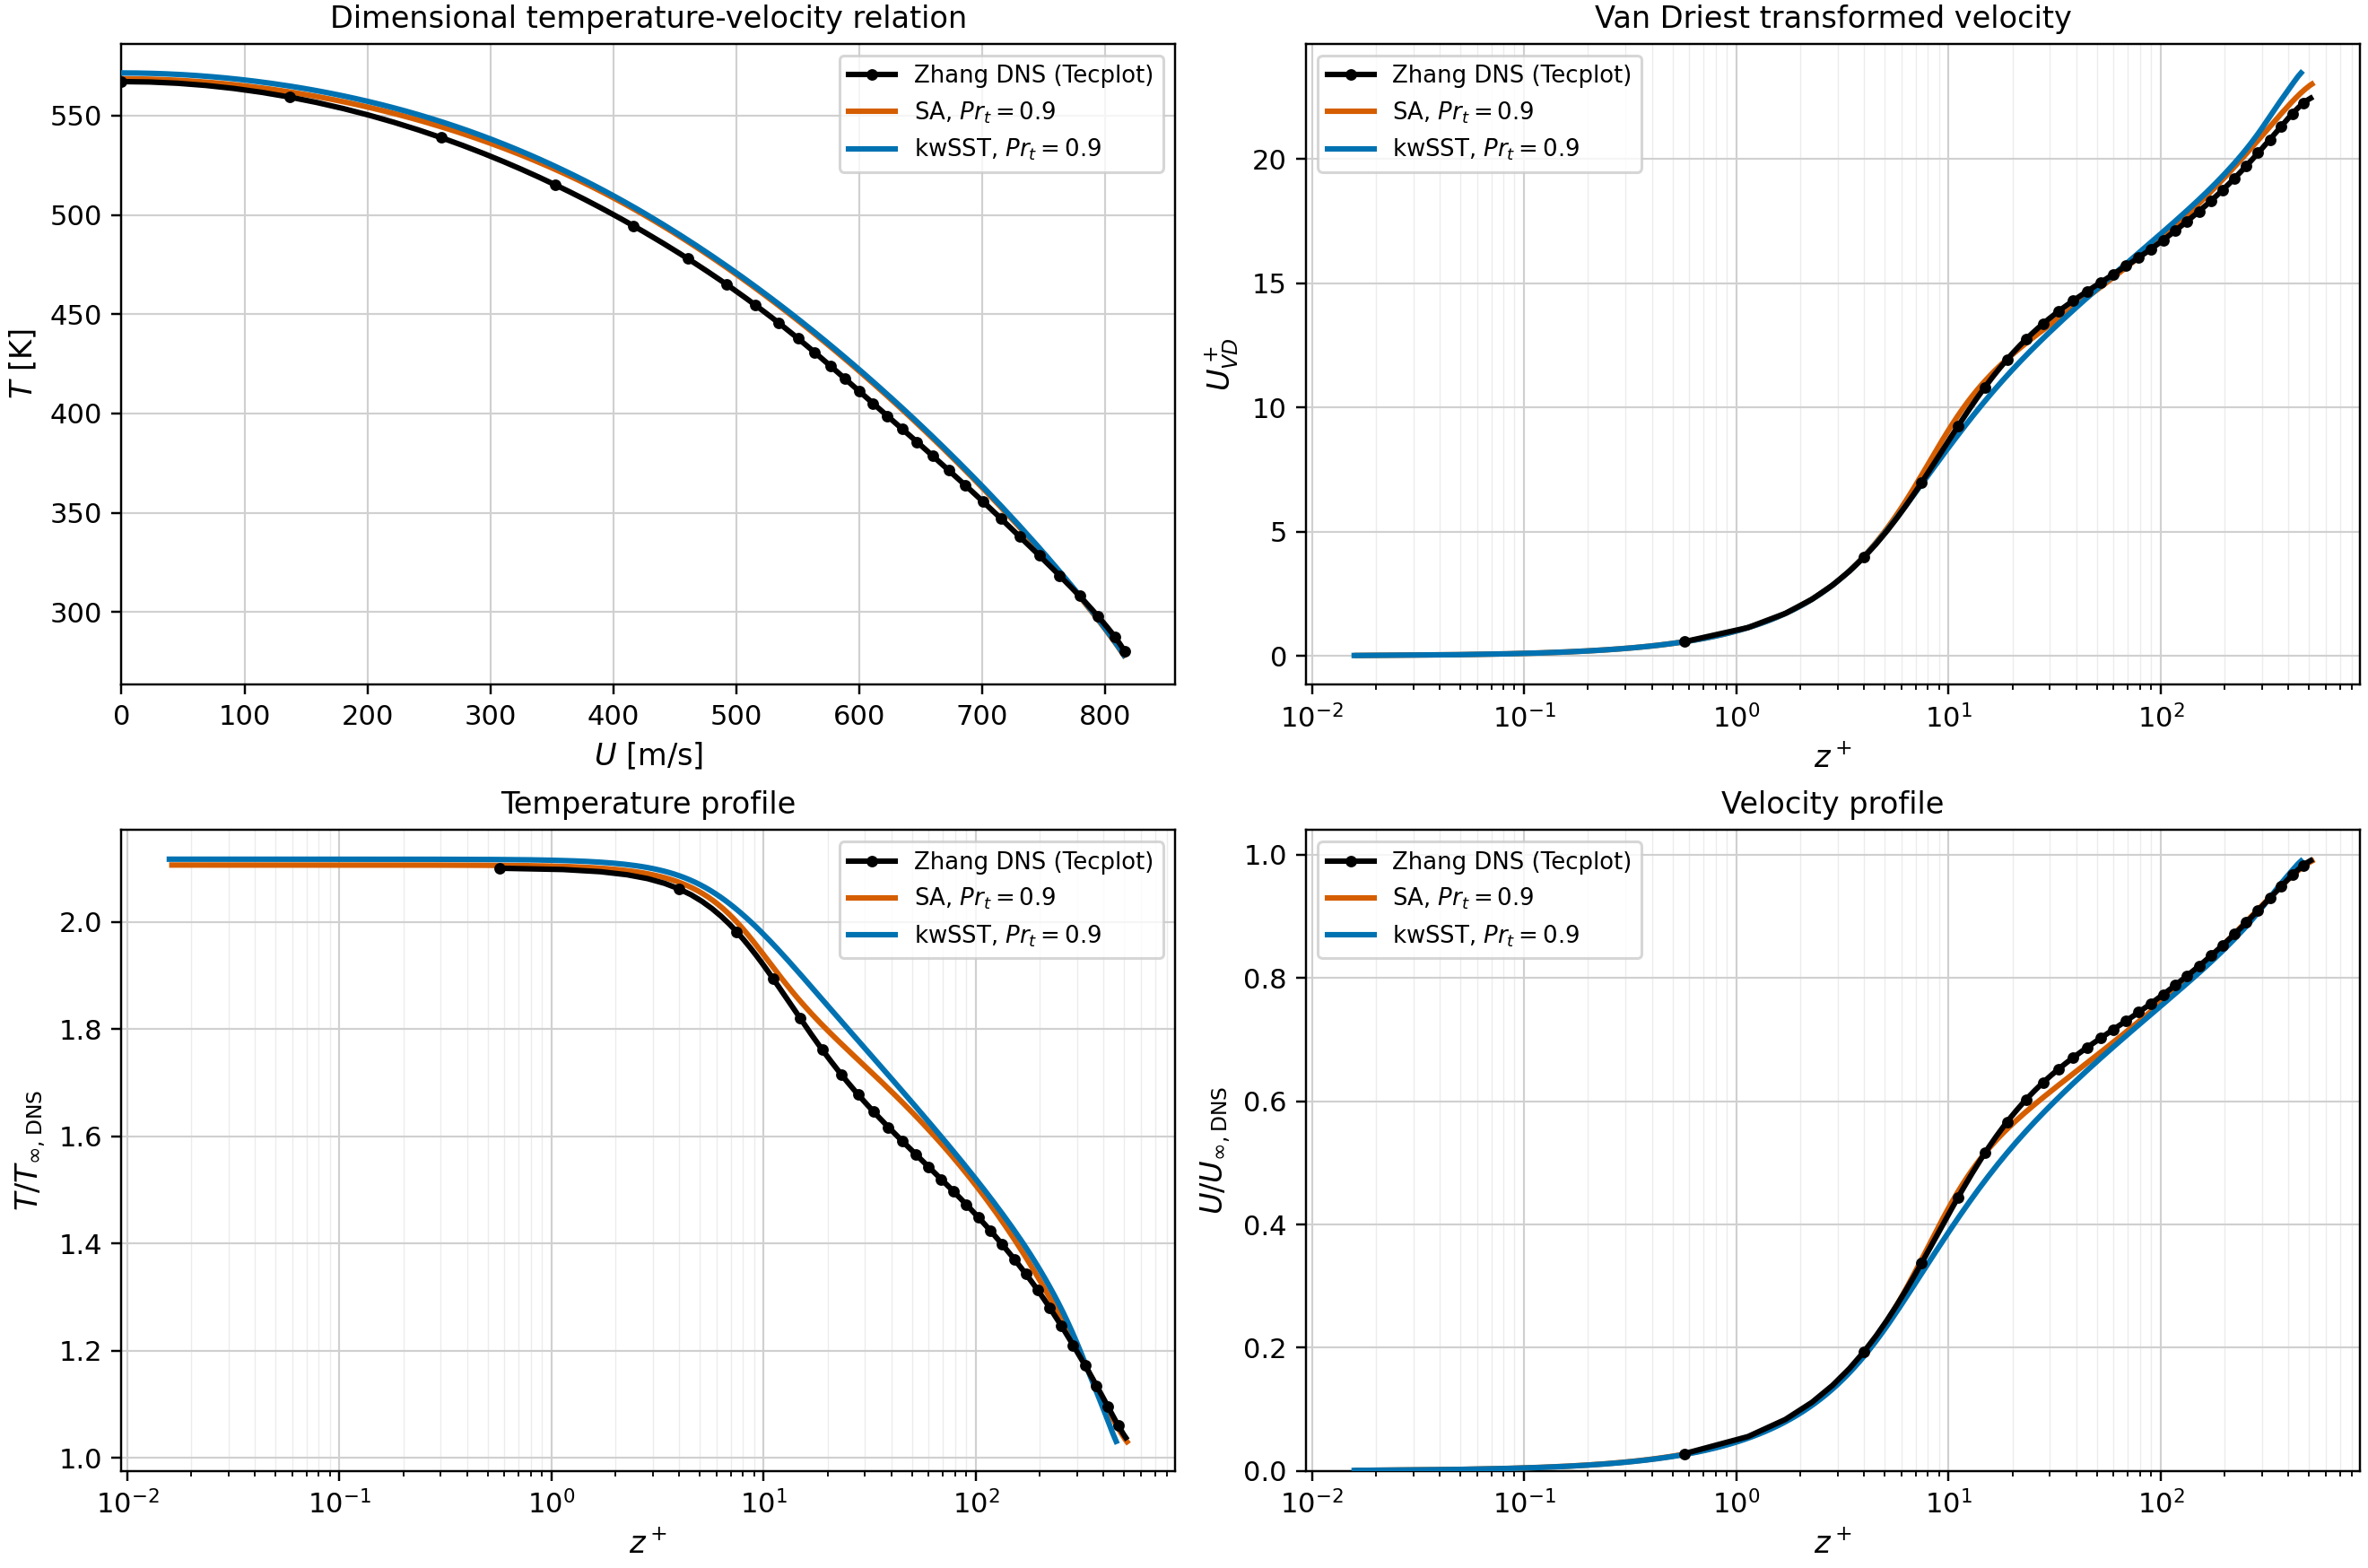
\includegraphics[width=\linewidth]{07_Error_Isolation_Results/Figures/Appendix/WR_BL_profile/M2p5_profiles.png}
    \caption[M2p5: wall-resolved boundary layer profiles]{Wall-resolved Spalart--Allmaras and \(k\)--\(\omega\) SST profiles for M2p5 at \(Pr_t=0.9\), compared with Zhang et al.'s DNS~\cite{zhang2018direct}. Top: dimensional \(T(U)\) (left) and van Driest--transformed velocity \(U_{\mathrm{VD}}^+\) versus \(z^+\) (right). Bottom: \(T/T_{\infty,\mathrm{DNS}}\) (left) and \(U/U_{\infty,\mathrm{DNS}}\) (right), both versus \(z^+\) at the matched \(Re_{\delta2}\) = 1657 station.}
    \label{fig:app:zpg:profiles:M2p5}
\end{figure}

\clearpage

\begin{figure}[!htbp]
    \centering
    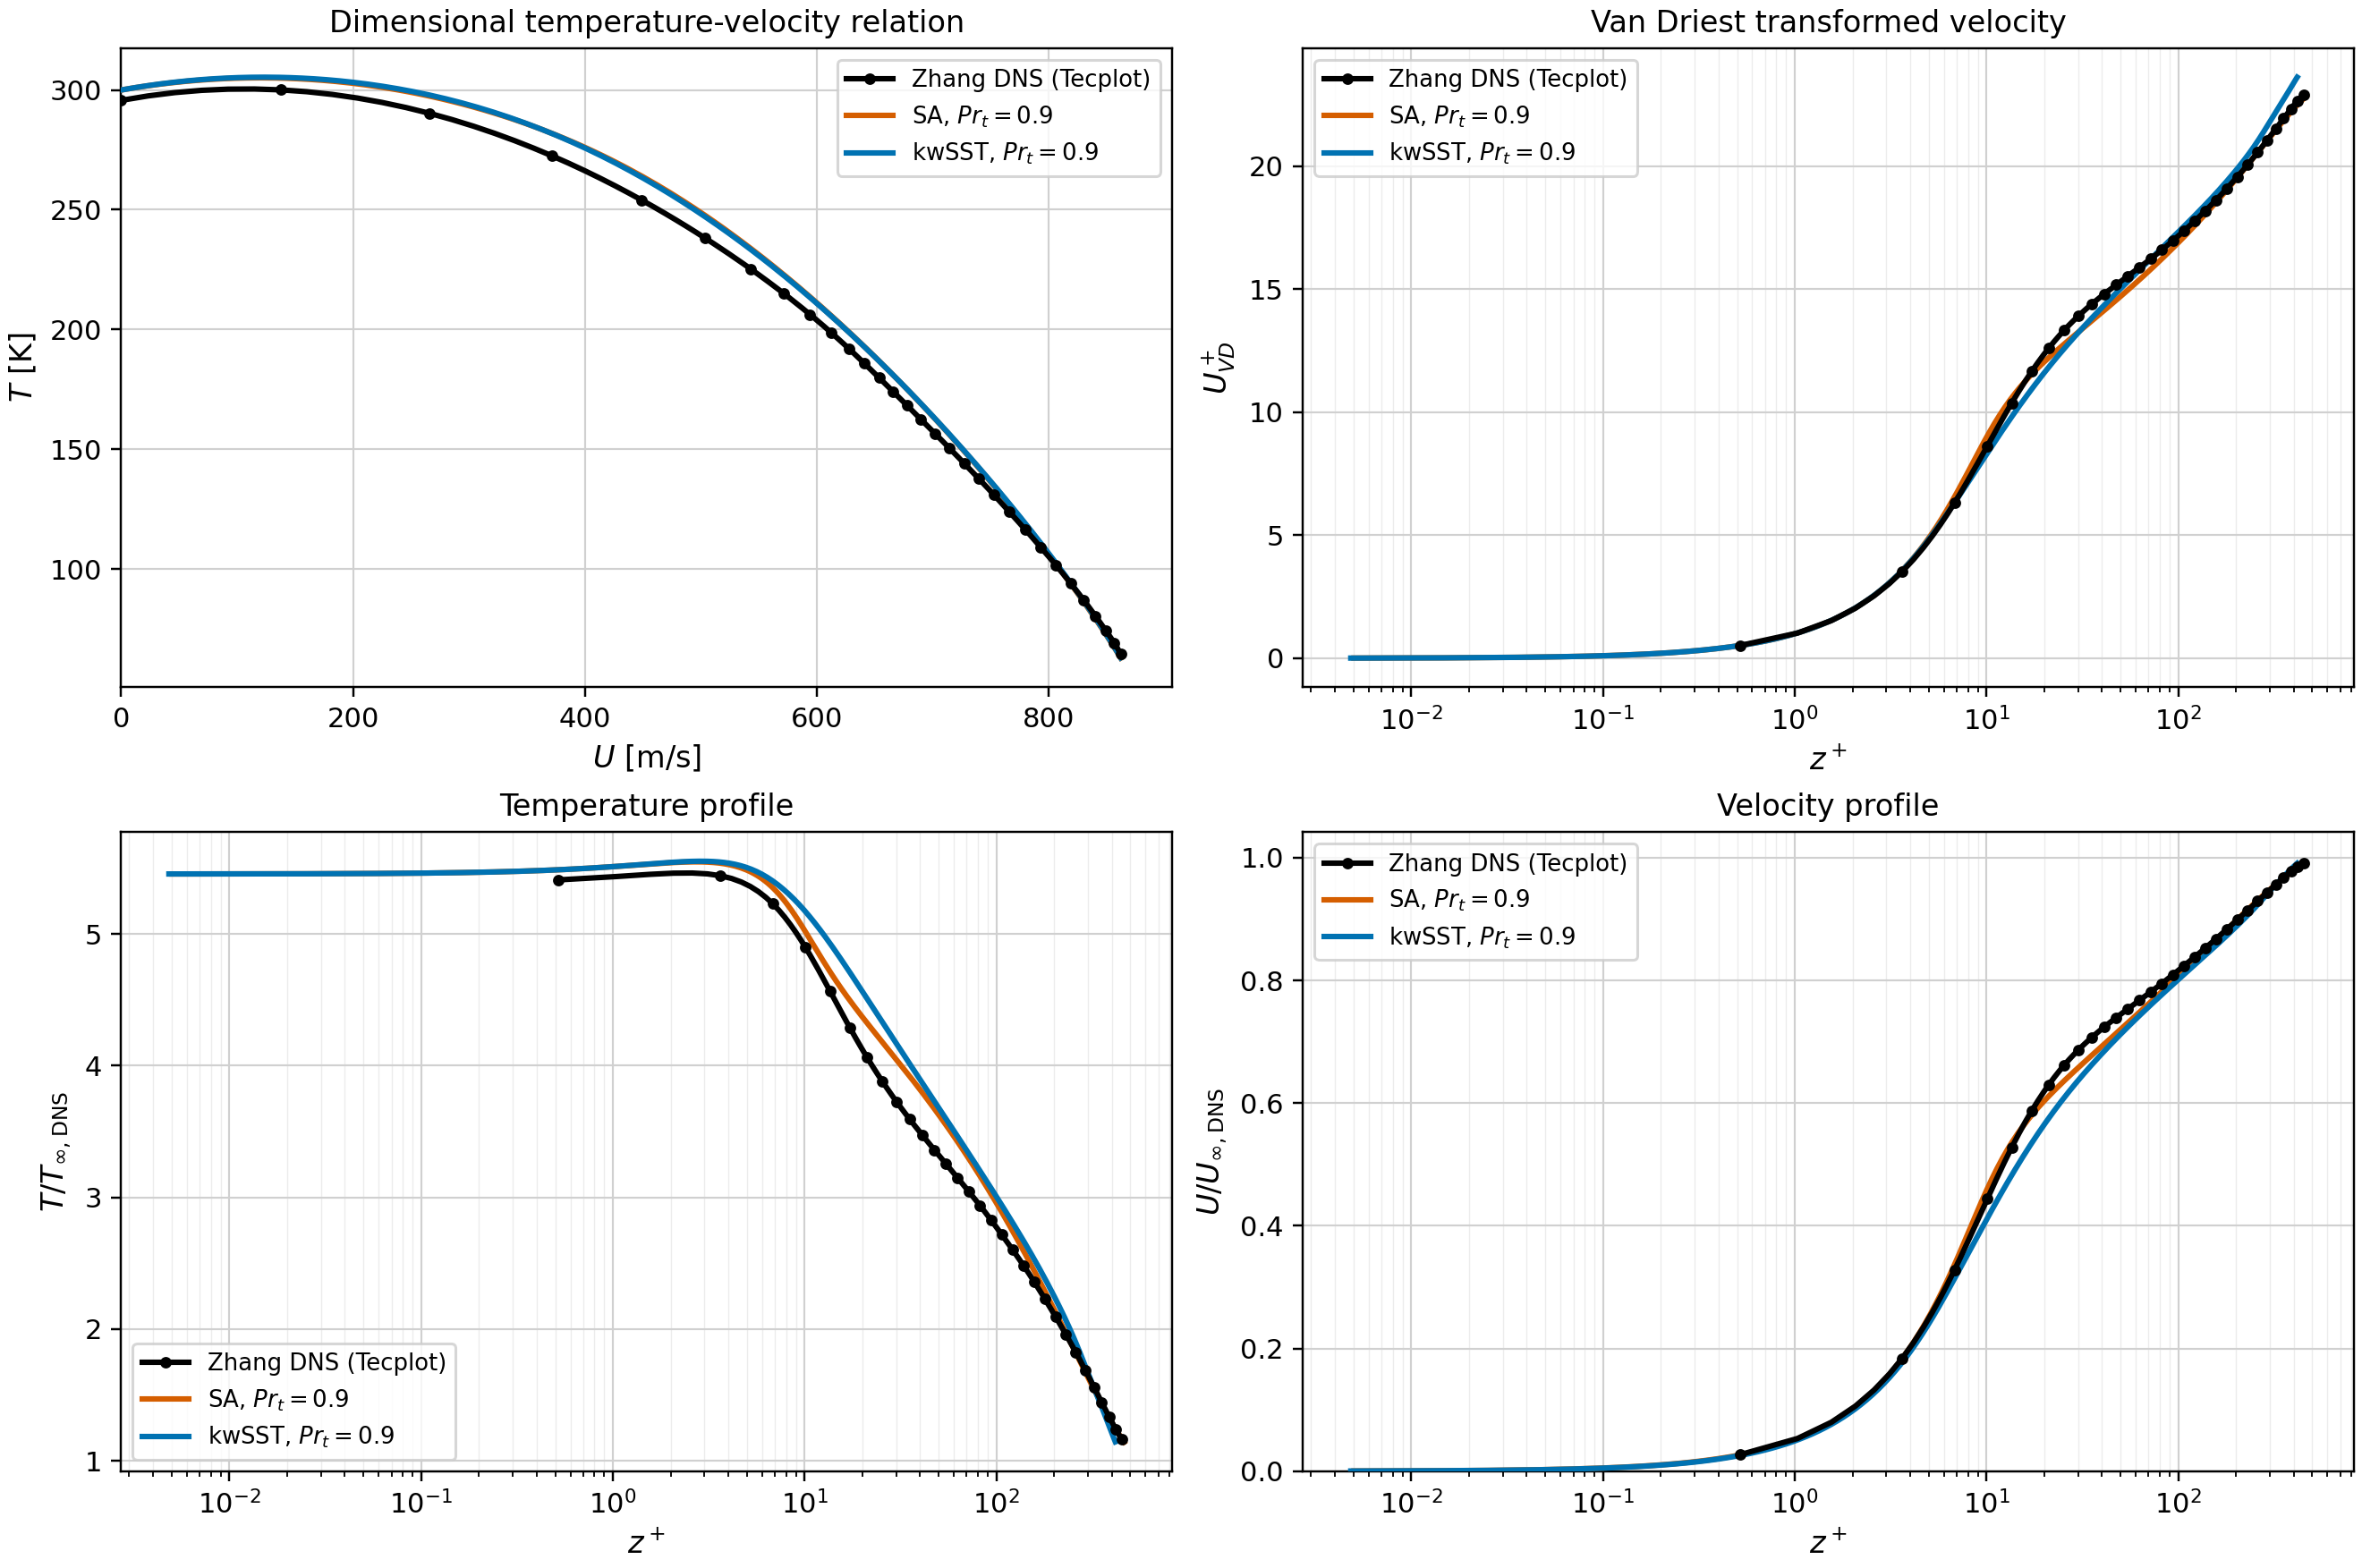
\includegraphics[width=\linewidth]{07_Error_Isolation_Results/Figures/Appendix/WR_BL_profile/M6Tw076_profiles.png}
    \caption[M6Tw076: wall-resolved boundary layer profiles]{Wall-resolved Spalart--Allmaras and \(k\)--\(\omega\) SST profiles for M6Tw076 at \(Pr_t=0.9\), compared with Zhang et al.'s DNS~\cite{zhang2018direct}. Top: dimensional \(T(U)\) (left) and van Driest--transformed velocity \(U_{\mathrm{VD}}^+\) versus \(z^+\) (right). Bottom: \(T/T_{\infty,\mathrm{DNS}}\) (left) and \(U/U_{\infty,\mathrm{DNS}}\) (right), both versus \(z^+\) at the matched \(Re_{\delta2}\) = 1746 station.}
    \label{fig:app:zpg:profiles:M6Tw076}
\end{figure}

\clearpage

\begin{figure}[!htbp]
    \centering
    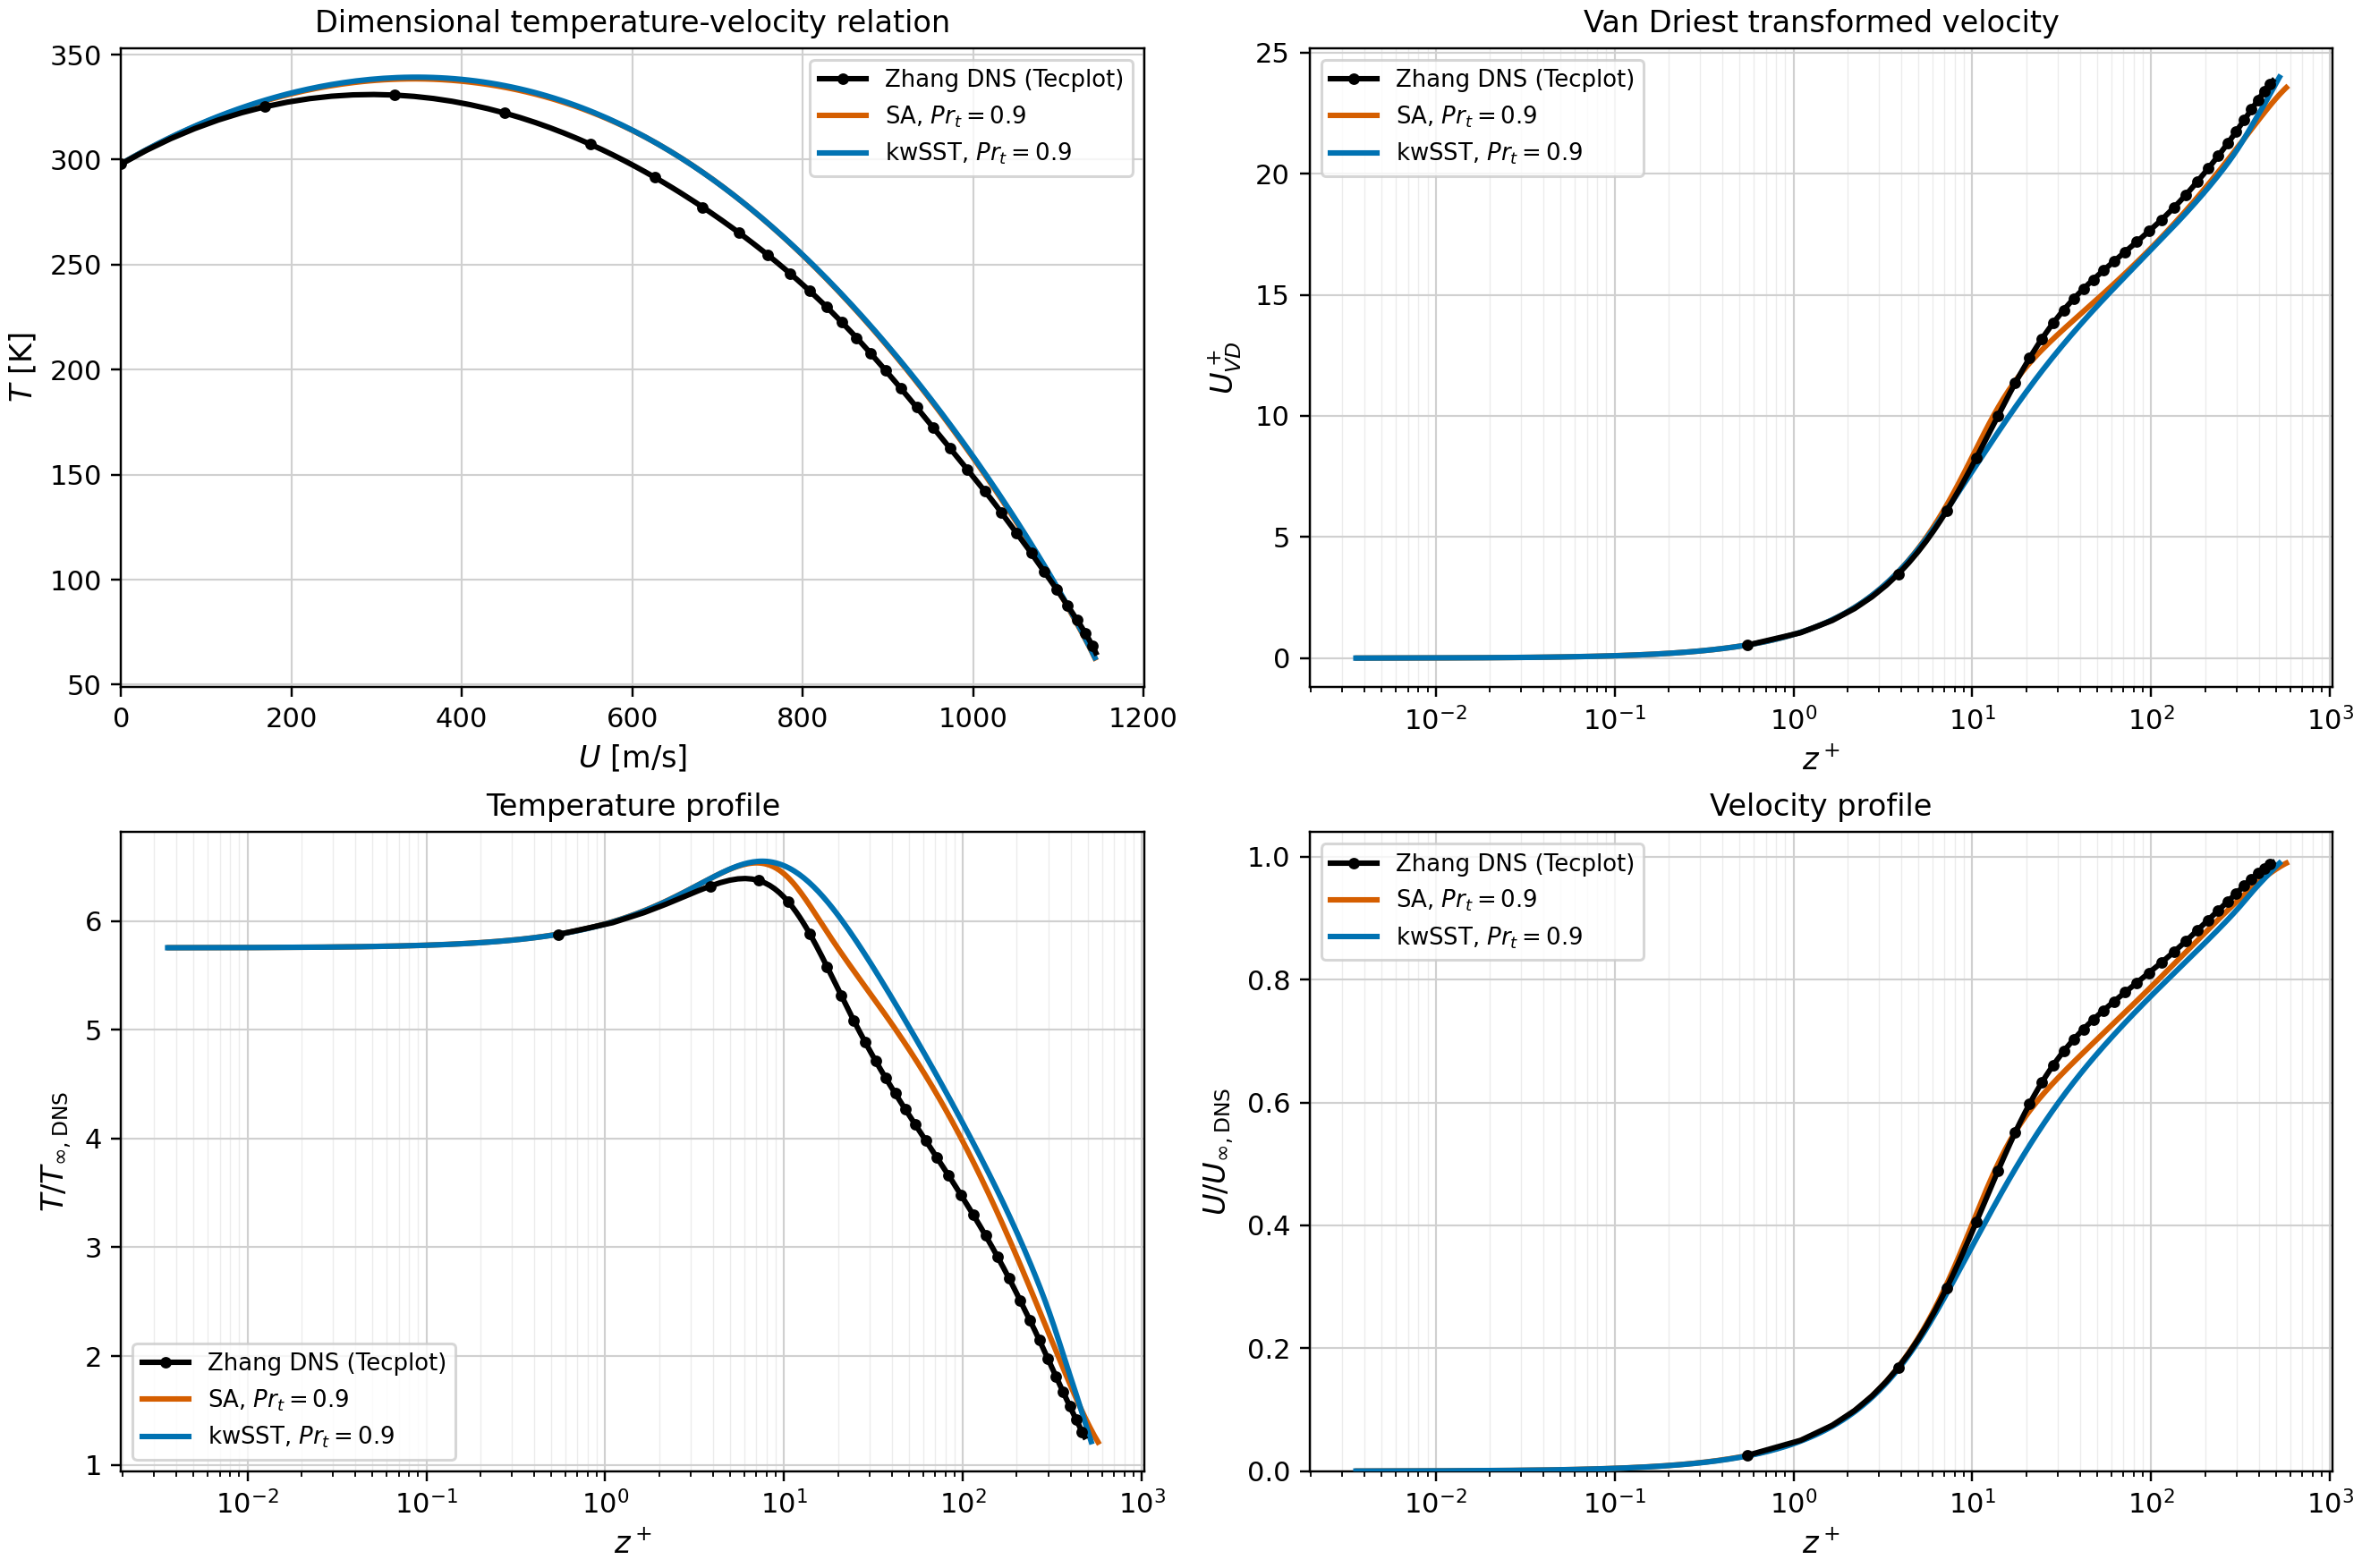
\includegraphics[width=\linewidth]{07_Error_Isolation_Results/Figures/Appendix/WR_BL_profile/M8Tw048_profiles.png}
    \caption[M8Tw048: wall-resolved boundary layer profiles]{Wall-resolved Spalart--Allmaras and \(k\)--\(\omega\) SST profiles for M8Tw048 at \(Pr_t=0.9\), compared with Zhang et al.'s DNS~\cite{zhang2018direct}. Top: dimensional \(T(U)\) (left) and van Driest--transformed velocity \(U_{\mathrm{VD}}^+\) versus \(z^+\) (right). Bottom: \(T/T_{\infty,\mathrm{DNS}}\) (left) and \(U/U_{\infty,\mathrm{DNS}}\) (right), both versus \(z^+\) at the matched \(Re_{\delta2}\) = 1990 station.}
    \label{fig:app:zpg:profiles:M8Tw048}
\end{figure}

\clearpage

\begin{figure}[!htbp]
    \centering
    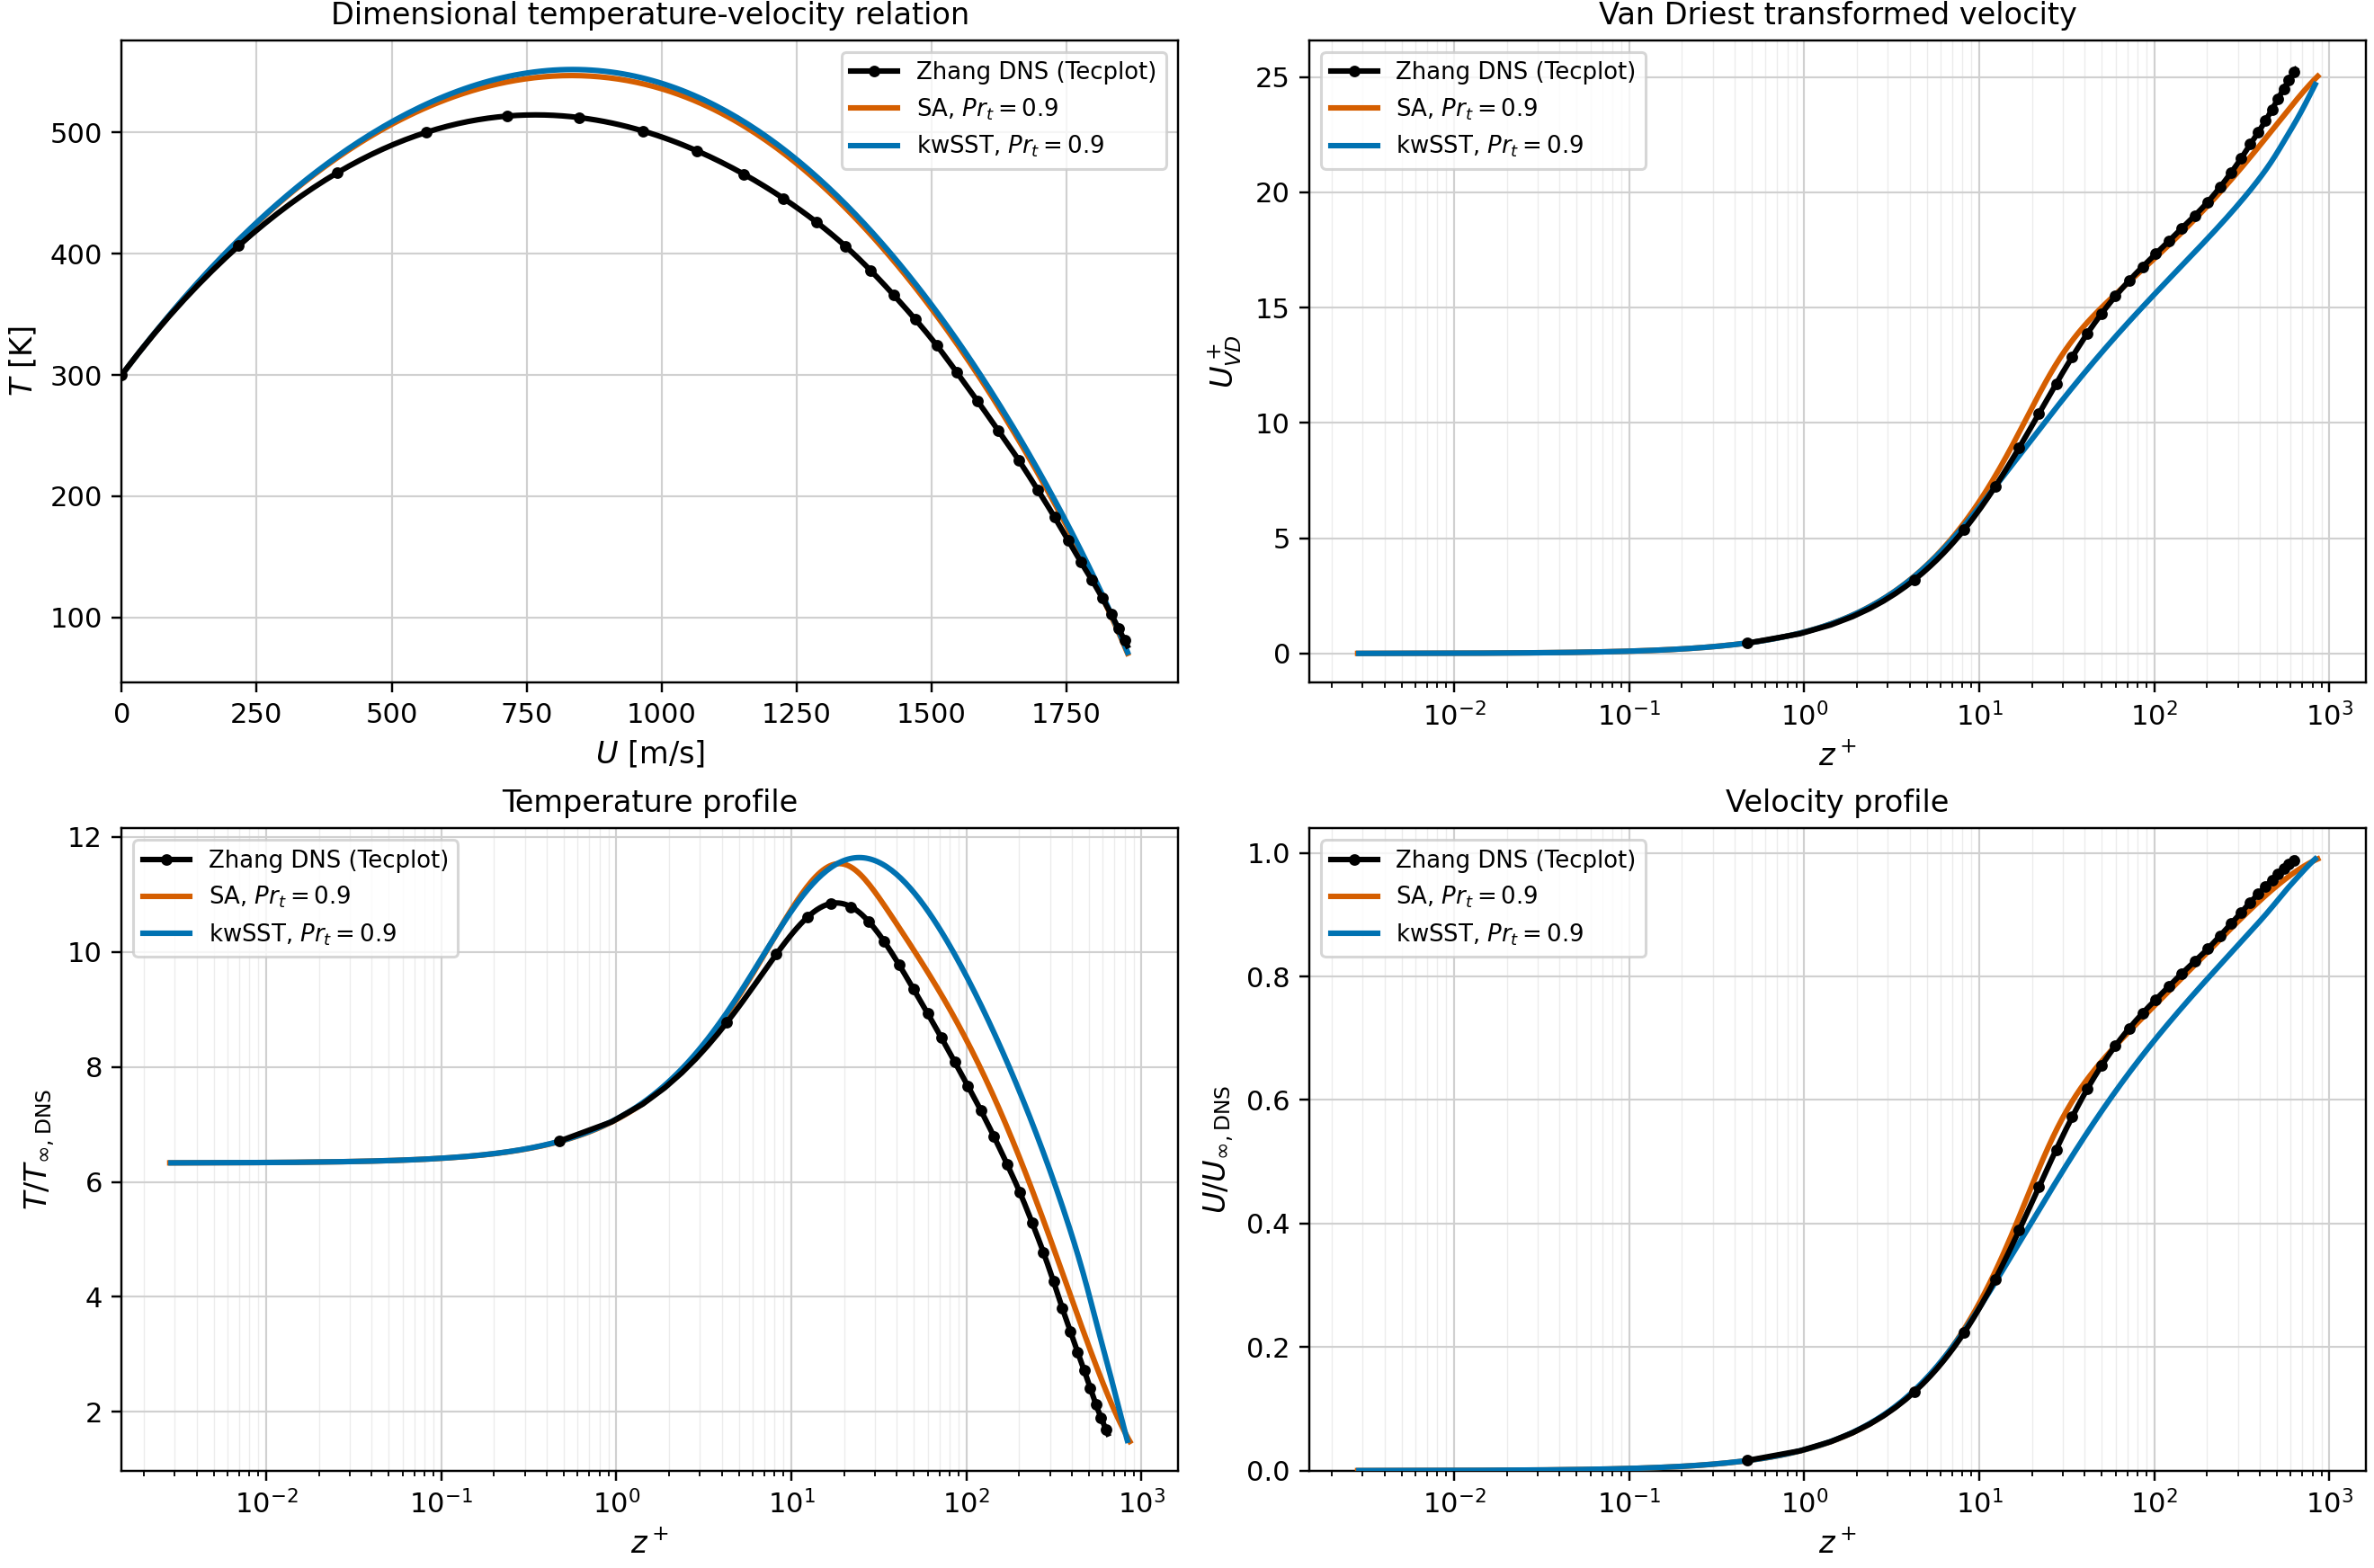
\includegraphics[width=\linewidth]{07_Error_Isolation_Results/Figures/Appendix/WR_BL_profile/M14Tw018_profiles.png}
    \caption[M14Tw018: wall-resolved boundary layer profiles]{Wall-resolved Spalart--Allmaras and \(k\)--\(\omega\) SST profiles for M14Tw018 at \(Pr_t=0.9\), compared with Zhang et al.'s DNS~\cite{zhang2018direct}. Top: dimensional \(T(U)\) (left) and van Driest--transformed velocity \(U_{\mathrm{VD}}^+\) versus \(z^+\) (right). Bottom: \(T/T_{\infty,\mathrm{DNS}}\) (left) and \(U/U_{\infty,\mathrm{DNS}}\) (right), both versus \(z^+\) at the matched \(Re_{\delta2}\) = 2354 station.}
    \label{fig:app:zpg:profiles:M14Tw018}
\end{figure}

\clearpage

\begin{landscape}
\section{Huang case at station BL2}

The Huang M11Tw020 case is represented by station BL2, this is the only of the three station for which the reference velocity and temperature profiles are available.

\begin{figure}[H]
    \centering
    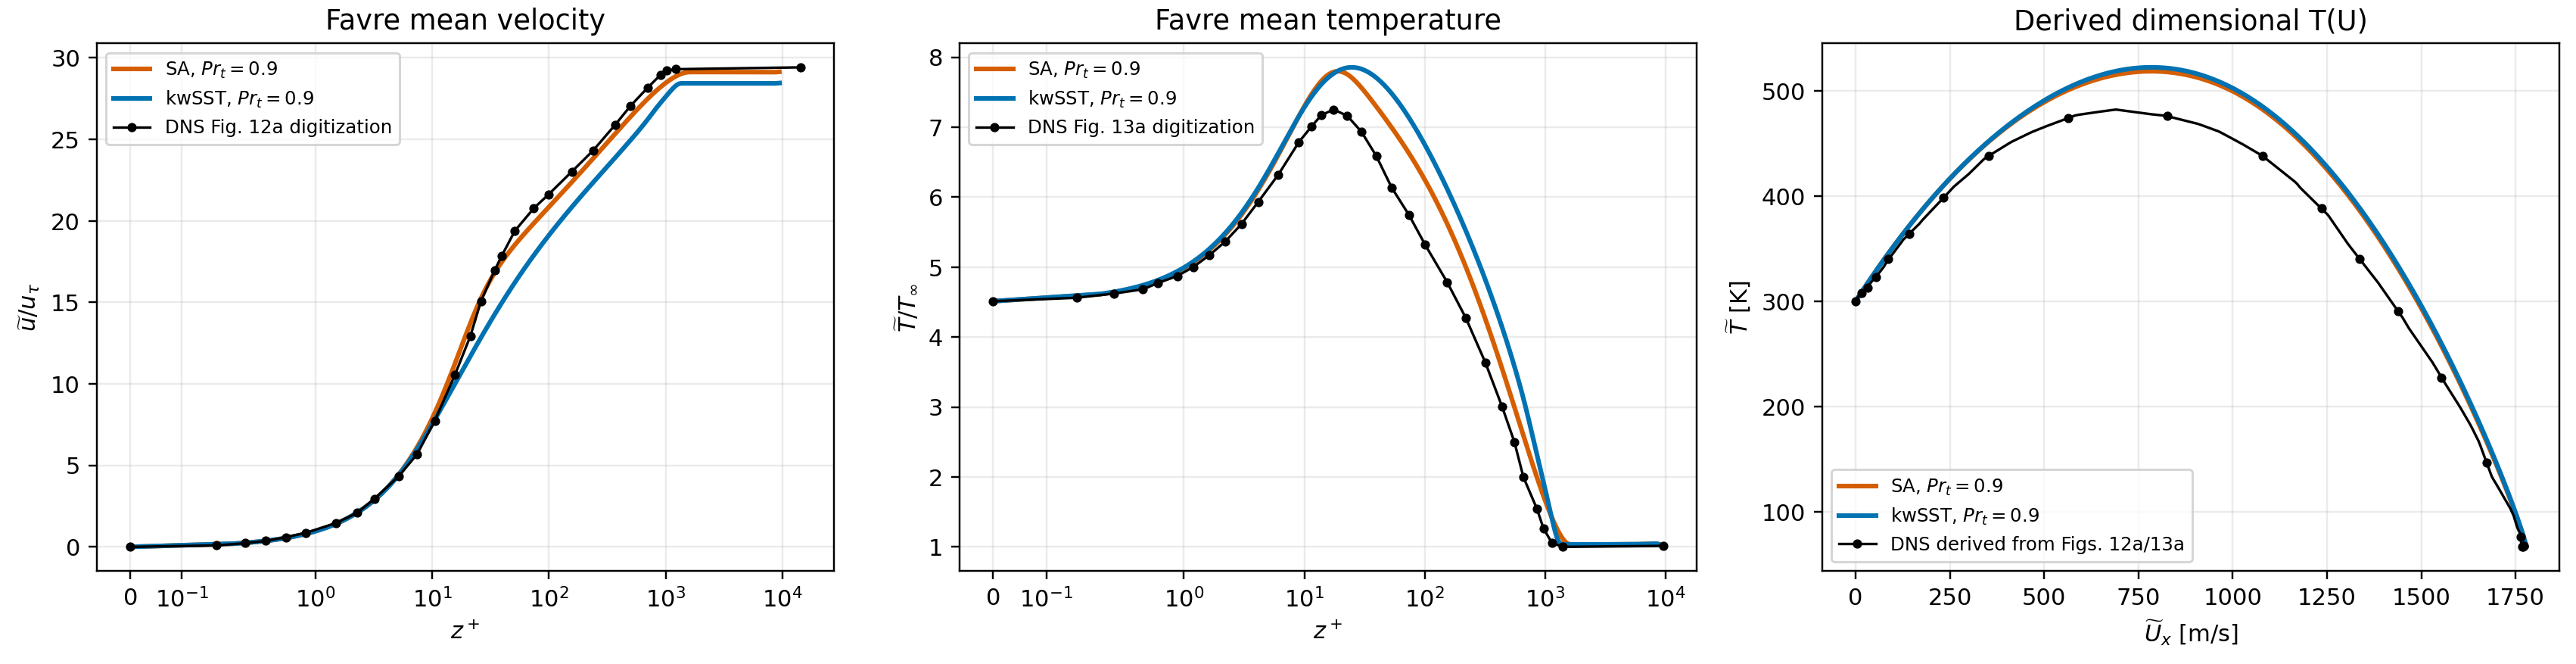
\includegraphics[width=\linewidth]{07_Error_Isolation_Results/Figures/Appendix/WR_BL_profile/Huang_BL2_profiles.png}
    \caption[Huang M11Tw020 at BL2: wall-resolved boundary layer profiles]{Wall-resolved Spalart--Allmaras and \(k\)--\(\omega\) SST profiles for M11Tw020 at station BL2 and \(Pr_t=0.9\), compared with DNS data digitized from Huang et al.~\cite[Figures~12(a) and 13(a)]{huang2020simulation}. Left: Favre-averaged velocity \(\widetilde{u}/u_\tau\) versus \(z^+\). Middle: temperature \(\widetilde{T}/T_\infty\) versus \(z^+\) at the matched \(Re_{\delta2}\) = 3419 station. Right: the corresponding dimensional temperature--velocity relation.}
    \label{fig:app:zpg:profiles:Huang-BL2}
\end{figure}

\end{landscape}

\chapter{A-priori wall-function assessments}
\label{app:zpg:apriori}

This appendix supplements Section~\ref{sec:comparative:zpg:cross-comparison}
with Li and Griffin assessments for the additional Zhang cases M2p5,
M6Tw076, M8Tw048 and M14Tw018. The prescribed-profile procedure is unchanged.
For adiabatic M2p5, relative heat-flux errors are undefined. The M6Tw076
heat-flux curves are retained for completeness, subject to the reference-data
limitations in Section~\ref{sec:evaluation:benchmark-cases}.

\section{Zhang cases}

% Figure provenance and reproducible replot for all eight assessments:
%   Script: 07_Error_Isolation_Results/Figures/Closures/plot_apriori_assessments.py
%   Exact saved solver sweeps, original WSL paths and SHA256 hashes:
%     07_Error_Isolation_Results/Figures/Closures/apriori_sources/manifest.json
%   Shear is shown left and heat flux right. The original 10.5 pt plotting
%   font and 0.85-linewidth inclusion are retained; each case occupies one page.

\begin{figure}[H]
    \centering
    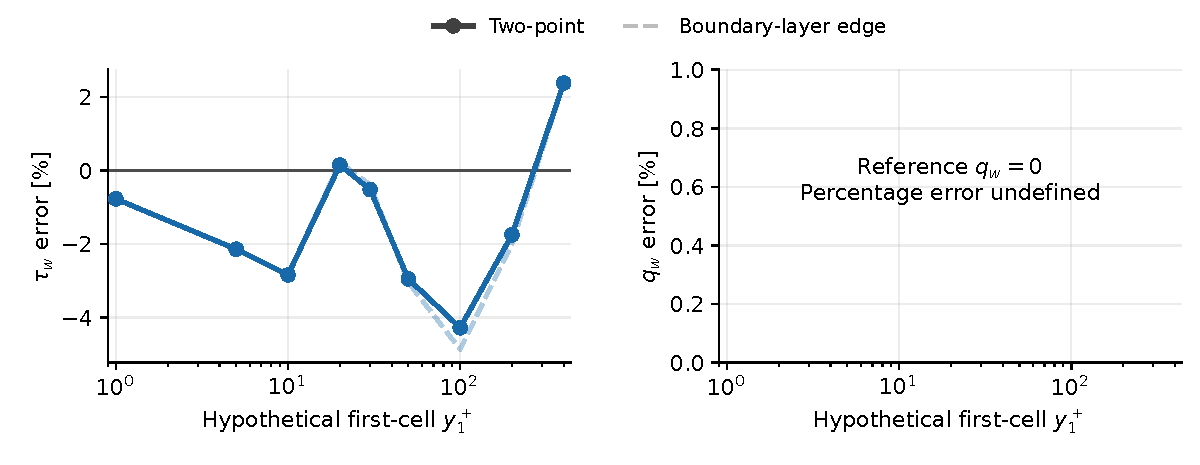
\includegraphics[width=0.85\linewidth]{07_Error_Isolation_Results/Figures/Appendix/a-priori/02_a-priori_Li_M2p5.pdf}
    \caption[M2p5: a-priori Li wall-function assessment]{A-priori Li assessment for M2p5; \(Re_\tau = 510\) \cite{zhang2018direct}. Signed relative errors in wall shear stress \(\tau_w\) (left) and heat-flux \(q_w\) (right) versus \(y_1^+\). Solid: equal-height two-cell formulation; dashed: boundary layer-edge reference. The heat-flux percentage error is undefined for this adiabatic reference.}
    \label{fig:app:zpg:apriori:Li-M2p5}
\end{figure}

\begin{figure}[H]
    \centering
    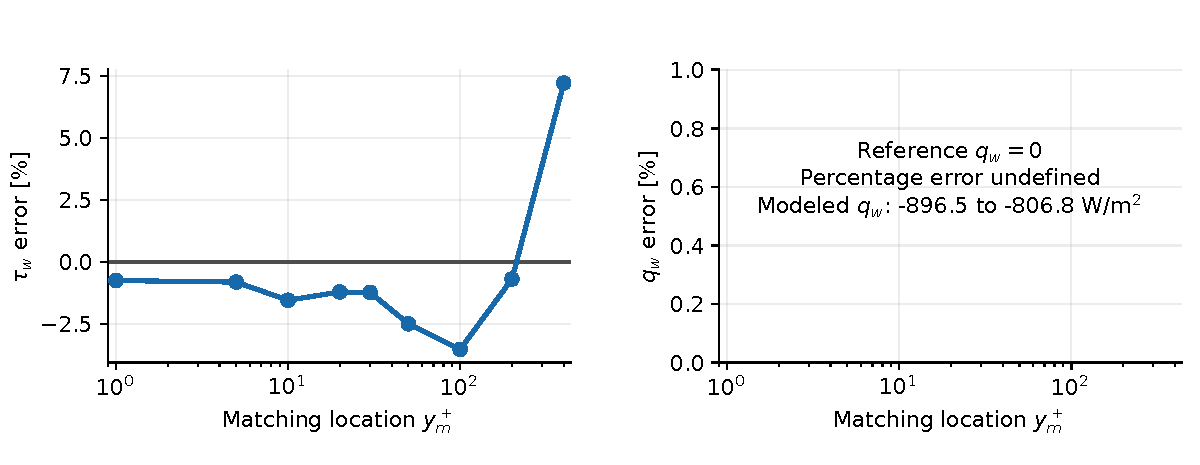
\includegraphics[width=0.85\linewidth]{07_Error_Isolation_Results/Figures/Appendix/a-priori/Griffin_M2p5.pdf}
    \caption[M2p5: a-priori Griffin wall-function assessment]{A-priori assessment of the Griffin wall function for M2p5; \(Re_\tau = 510\) \cite{zhang2018direct}. Signed relative errors in wall shear stress \(\tau_w\) (left) and wall heat-flux \(q_w\) (right) versus matching height \(y_m^+\). The relative heat-flux error is undefined because the reference heat-flux is zero.}
    \label{fig:app:zpg:apriori:Griffin-M2p5}
\end{figure}

\clearpage

\begin{figure}[H]
    \centering
    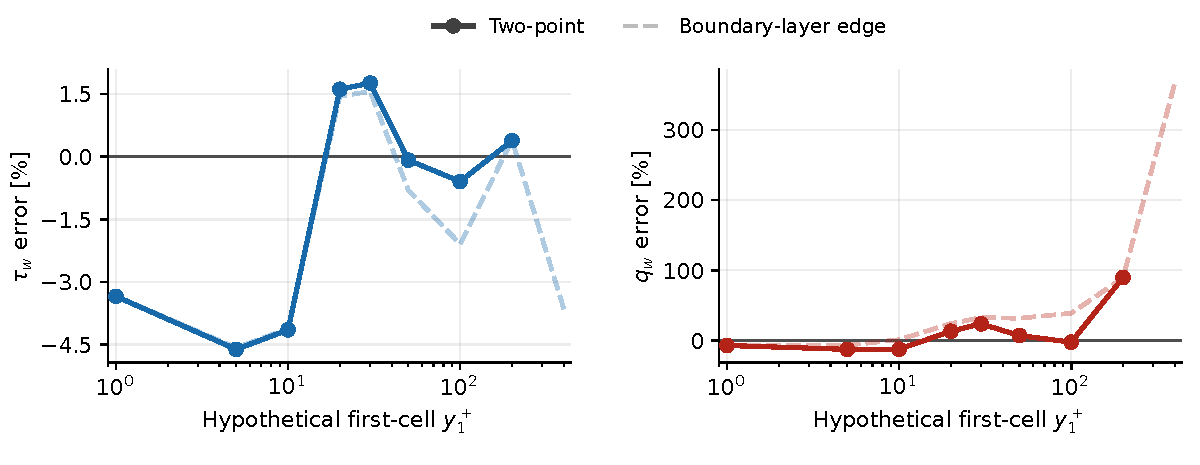
\includegraphics[width=0.85\linewidth]{07_Error_Isolation_Results/Figures/Appendix/a-priori/02_a-priori_Li_M6Tw076.pdf}
    \caption[M6Tw076: a-priori Li wall-function assessment]{A-priori assessment of the Li wall function for M6Tw076; \(Re_\tau = 453\) \cite{zhang2018direct}. Signed relative errors in wall shear stress \(\tau_w\) (left) and wall heat-flux \(q_w\) (right) versus virtual first-cell height \(y_1^+\). Solid curves use the equal-height two-cell formulation; dashed curves use the boundary layer-edge reference. The heat-flux curves are shown for completeness and excluded from quantitative assessment against DNS.}
    \label{fig:app:zpg:apriori:Li-M6Tw076}
\end{figure}

\begin{figure}[H]
    \centering
    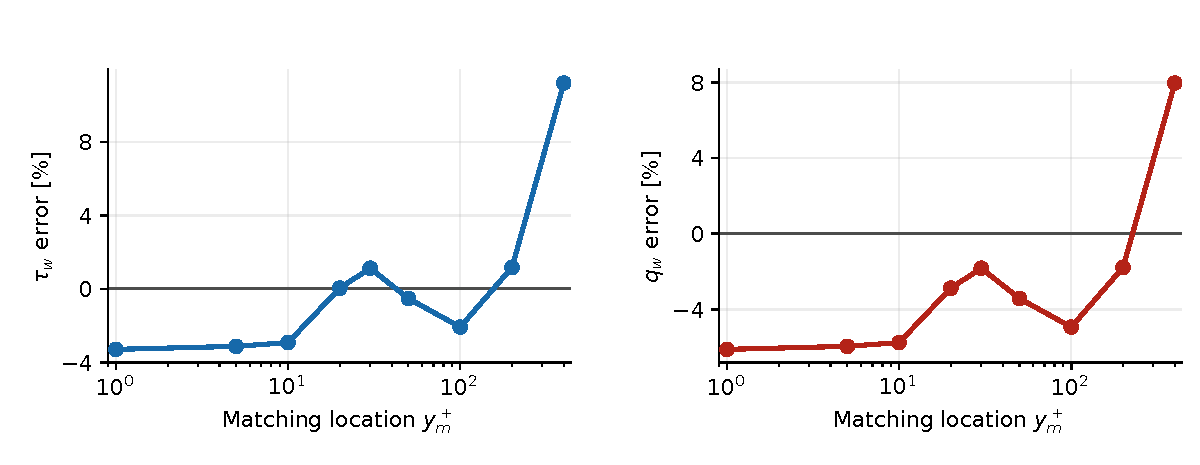
\includegraphics[width=0.85\linewidth]{07_Error_Isolation_Results/Figures/Appendix/a-priori/Griffin_M6Tw076.pdf}
    \caption[M6Tw076: a-priori Griffin wall-function assessment]{A-priori assessment of the Griffin wall function for M6Tw076; \(Re_\tau = 453\) \cite{zhang2018direct}. Signed relative errors in wall shear stress \(\tau_w\) (left) and wall heat-flux \(q_w\) (right) versus matching height \(y_m^+\). The heat-flux curves are shown for completeness and excluded from quantitative assessment against DNS.}
    \label{fig:app:zpg:apriori:Griffin-M6Tw076}
\end{figure}

\clearpage

\begin{figure}[H]
    \centering
    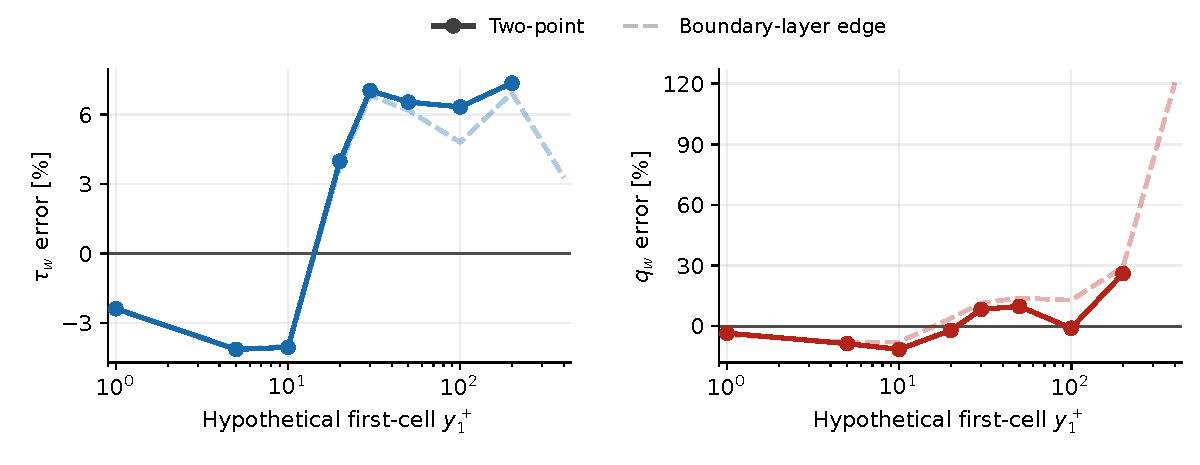
\includegraphics[width=0.85\linewidth]{07_Error_Isolation_Results/Figures/Appendix/a-priori/02_a-priori_Li_M8Tw048.pdf}
    \caption[M8Tw048: a-priori Li wall-function assessment]{A-priori assessment of the Li wall function for M8Tw048; \(Re_\tau = 480\) \cite{zhang2018direct}. Signed relative errors in wall shear stress \(\tau_w\) (left) and wall heat-flux \(q_w\) (right) versus virtual first-cell height \(y_1^+\). Solid curves use the equal-height two-cell formulation; dashed curves use the boundary layer-edge reference.}
    \label{fig:app:zpg:apriori:Li-M8Tw048}
\end{figure}

\begin{figure}[H]
    \centering
    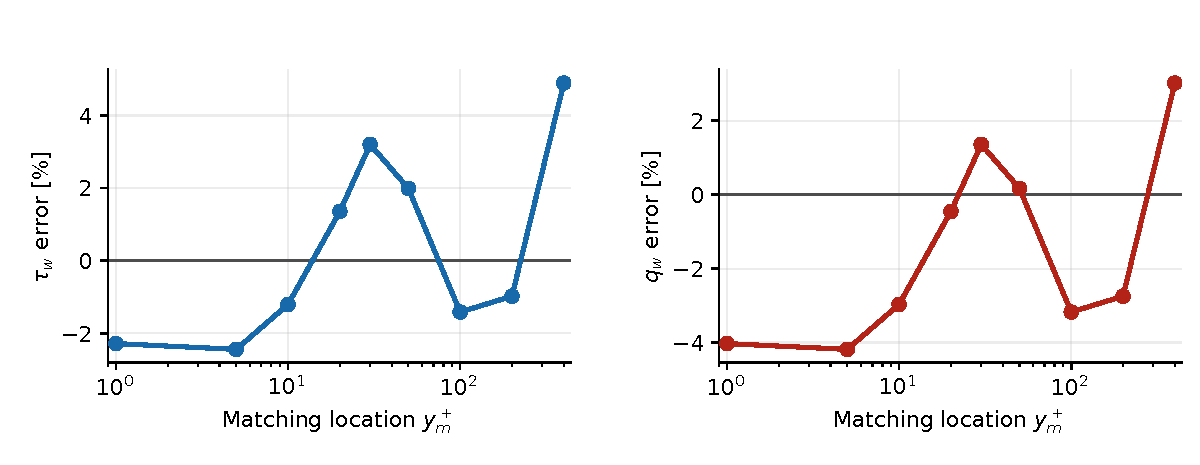
\includegraphics[width=0.85\linewidth]{07_Error_Isolation_Results/Figures/Appendix/a-priori/Griffin_M8Tw048.pdf}
    \caption[M8Tw048: a-priori Griffin wall-function assessment]{A-priori assessment of the Griffin wall function for M8Tw048; \(Re_\tau = 480\) \cite{zhang2018direct}. Signed relative errors in wall shear stress \(\tau_w\) (left) and wall heat-flux \(q_w\) (right) versus matching height \(y_m^+\).}
    \label{fig:app:zpg:apriori:Griffin-M8Tw048}
\end{figure}

\clearpage

\begin{figure}[H]
    \centering
    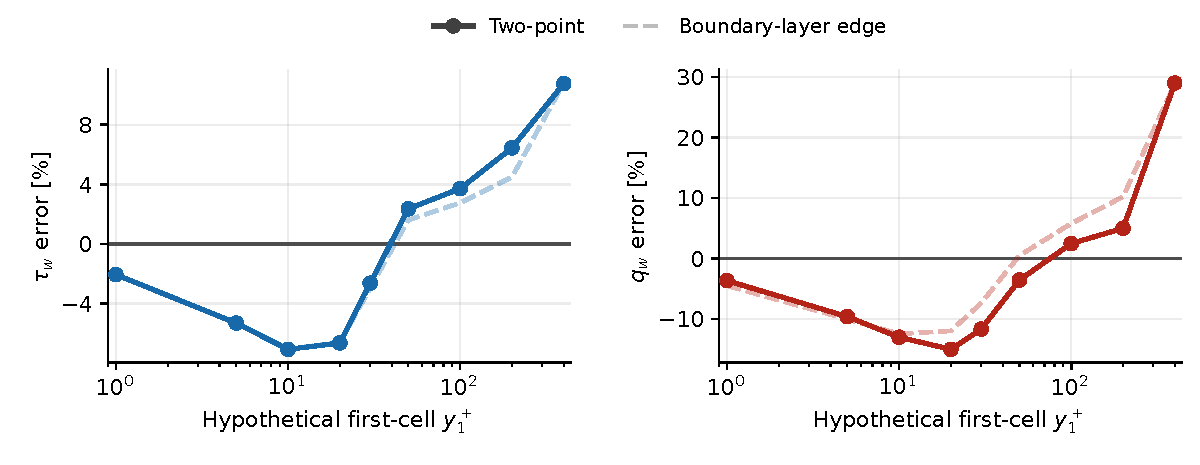
\includegraphics[width=0.85\linewidth]{07_Error_Isolation_Results/Figures/Appendix/a-priori/02_a-priori_Li_M14Tw018.pdf}
    \caption[M14Tw018: a-priori Li wall-function assessment]{A-priori assessment of the Li wall function for M14Tw018; \(Re_\tau = 646\) \cite{zhang2018direct}. Signed relative errors in wall shear stress \(\tau_w\) (left) and wall heat-flux \(q_w\) (right) versus virtual first-cell height \(y_1^+\). Solid curves use the equal-height two-cell formulation; dashed curves use the boundary layer-edge reference.}
    \label{fig:app:zpg:apriori:Li-M14Tw018}
\end{figure}

\begin{figure}[H]
    \centering
    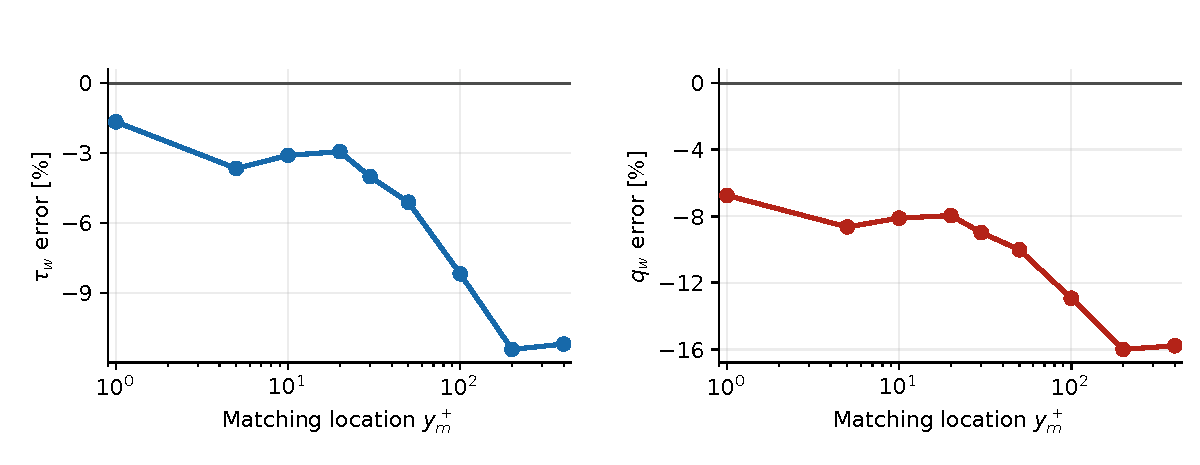
\includegraphics[width=0.85\linewidth]{07_Error_Isolation_Results/Figures/Appendix/a-priori/Griffin_M14Tw018.pdf}
    \caption[M14Tw018: a-priori Griffin wall-function assessment]{A-priori assessment of the Griffin wall function for M14Tw018; \(Re_\tau = 646\) \cite{zhang2018direct}. Signed relative errors in wall shear stress \(\tau_w\) (left) and wall heat-flux \(q_w\) (right) versus matching height \(y_m^+\).}
    \label{fig:app:zpg:apriori:Griffin-M14Tw018}
\end{figure}


% Thesis-native adaptation; the unmodified report is in source_as_supplied/.
% The chapter is included after the main document's \appendix command.
\chapter{Sutherland-law coefficient in Malik and Anderson (1991)}
\label{app:malik-anderson-sutherland}

\begingroup
\definecolor{MAAppBlue}{HTML}{17324D}
\definecolor{MAAppSteel}{HTML}{456C86}
\definecolor{MAAppLightBlue}{HTML}{EAF2F7}
\definecolor{MAAppLightGreen}{HTML}{EAF6EF}
\definecolor{MAAppLightRed}{HTML}{FBEDEC}
\definecolor{MAAppGray}{HTML}{F5F7F9}
\definecolor{MAAppRule}{HTML}{D8E0E6}

\newcommand{\maAppName}{Malik--Anderson}
\newcommand{\maAppDd}{\mathrm{d}}
\newcommand{\maAppUe}{u_e}
\newcommand{\maAppTe}{T_e}
\newcommand{\maAppRhoe}{\rho_e}
\newcommand{\maAppMue}{\mu_e}
\newcommand{\maAppCpe}{c_{p,e}}
\newcommand{\maAppPrzero}{Pr_0}

\newcommand{\maAppNote}[2]{%
  \vspace{0.3em}%
  \noindent\colorbox{#1}{%
    \begin{minipage}{\dimexpr\linewidth-2\fboxsep\relax}
      #2
    \end{minipage}}%
  \vspace{0.3em}%
}

\newcommand{\maAppEqbox}[2]{%
  \vspace{0.1em}%
  \noindent\fcolorbox{MAAppRule}{#1}{%
    \begin{minipage}{\dimexpr\linewidth-2\fboxsep-2\fboxrule\relax}
      #2
    \end{minipage}}%
  \vspace{0.1em}%
}

\section{Summary}
\label{app:ma:sec:short_conclusion}
This appendix concerns M.~R. Malik and E.~C. Anderson, ``Real gas effects on hypersonic boundary-layer stability,'' \emph{Physics of Fluids A} \textbf{3}, 803--821 (1991), \href{https://doi.org/10.1063/1.858012}{\nolinkurl{doi:10.1063/1.858012}}~\cite{MalikAnderson1991RealGas}. Their Eq.~(56) states the Sutherland law
\[
  \mu(T)=d_1\frac{\sqrt{T}}{1+d_2/T},
  \qquad d_2=110~\mathrm{K},
\]
with \(d_{1,\mathrm{print}}=1.0869\times10^{-6}\). When \(T\) is measured in kelvin and \(\mu\) in SI units, dimensional consistency requires
\[
  [d_1]=\mathrm{kg\,m^{-1}\,s^{-1}\,K^{-1/2}}.
\]
The unit printed with Eq.~(56) omits the factor \(\mathrm{K^{-1/2}}\); this dimensional typo is separate from the numerical-coefficient inconsistency investigated here.

The Mach-15 calorically imperfect mean-flow profiles in Fig.~3 cannot be reproduced with the printed coefficient under the stated Sutherland, Keyes, and Eggers closures. The tested candidate \(d_{1,\mathrm{cand}}=1.5869\times10^{-6}\,\mathrm{kg\,m^{-1}\,s^{-1}\,K^{-1/2}}\) gives substantially closer agreement with the digitized Fig.~3 profiles. Analytically, the distinction is consistent: the Sutherland constant \(d_1\) cancels from the Reynolds-normalized perfect-gas similarity problem, whereas it remains in the calorically imperfect energy equation through the thermal-diffusion coefficient \(K\propto d_1^{-1}\).

\maAppNote{MAAppLightBlue}{%
\begin{itemize}
    \item \textbf{Strong indication of a typo:} the printed coefficient in Eq.~(56) is inconsistent with the calorically imperfect mean-flow profiles in Fig.~3, whereas \(d_1=1.5869\times10^{-6}\) gives substantially closer agreement. This strongly indicates a typographical or implementation inconsistency, although the exact replacement value is not uniquely established by the digitized profiles.
    \item \textbf{Perfect-gas cases are unaffected:} although they use the same Sutherland law, \(d_1\) cancels from the Reynolds-normalized perfect-gas similarity equations and from the plotted wall coordinate. This appendix demonstrates the cancellation analytically and confirms it with the profile reproductions.
    \item \textbf{Real-gas cases are unaffected by Eq.~(56):} the real-gas calculations, which form the main contribution of the paper, use a Wilke mixture-viscosity model instead of the disputed Sutherland coefficient. They are therefore outside the direct scope of this inconsistency.
    \item \textbf{Figure 13 remains unresolved:} Fig.~13 includes a calorically imperfect stability curve and may therefore be affected. Neither its perfect-gas nor its imperfect-gas curve was reproduced here, so no conclusion is drawn about the magnitude or direction of a possible effect.
\end{itemize}
}

\subsection*{Outline}

\begin{itemize}
    \item Section~\ref{app:ma:sec:wall_coordinate} shows that the discrepancy does not originate in the length scale. Reconstructing $y$ from the Levy--Lees similarity coordinate $\eta$ and then normalizing it as $Y=y/L_r$ introduces no explicit dependence on $d_1$: the factor cancels.
    \item Section~\ref{app:ma:sec:perfect_gas_similarity} shows that the Reynolds-normalized perfect-gas profiles are independent of $d_1$. The momentum and energy similarity equations contain no explicit $d_1$.
    \item Section~\ref{app:ma:sec:imperfect_gas_similarity} shows why the calorically imperfect profiles do depend on $d_1$. The thermal-diffusion coefficient satisfies $K\propto 1/d_1$, so $d_1$ affects the temperature profile directly and the velocity profile through the coupled similarity equations.
    \item Section~\ref{app:ma:sec:profile_validation_plots} compares the perfect- and calorically imperfect-gas solutions with the digitized profiles from Fig.~3 of Malik and Anderson. For the Mach-15 calorically imperfect case, the candidate $d_{1,\mathrm{cand}}=1.5869\times10^{-6}$ is substantially more consistent with the published profiles than the printed value. A non-converged printed-coefficient marching attempt is also shown as a visual diagnostic; neither comparison is a unique fit of the exact replacement value.
\end{itemize}

The detailed mathematical derivations are given in Sections~\ref{app:ma:sec:similarity_coefficients}--\ref{app:ma:sec:K_dependence} and referenced throughout this appendix.

\section{\maAppName{} property setup}
\label{app:ma:sec:property_setup}

The paper gives the Sutherland viscosity law as Eq.~(56)~\cite{MalikAnderson1991RealGas}:
\begin{equation}
  \mu(T)
  = d_1 \frac{\sqrt{T}}{1+d_2/T}
  = d_1 \frac{T^{3/2}}{T+d_2},
  \qquad d_2 = 110~\mathrm{K}.
  \label{app:ma:eq:sutherland}
\end{equation}

The printed and candidate values compared in this appendix are
\begin{align}
  d_{1,\mathrm{print}}&=1.0869\times10^{-6}~\mathrm{kg\,m^{-1}\,s^{-1}\,K^{-1/2}},\\
  d_{1,\mathrm{cand}}&=1.5869\times10^{-6}~\mathrm{kg\,m^{-1}\,s^{-1}\,K^{-1/2}}.
\end{align}
The second value is treated as a tested candidate, not as a uniquely fitted correction.

\maAppEqbox{MAAppGray}{%
\textbf{\maAppName{} Mach 10 / 15 "perfect"-gas model}
\begin{align}
  p &= \rho R T, &
  c_p &= \mathrm{const.}, &
  \maAppPrzero &= 0.7, &
  k &= \frac{\mu c_p}{\maAppPrzero}.
\end{align}
}


\maAppEqbox{MAAppGray}{%
\textbf{\maAppName{} Mach 15 "imperfect"-gas model}
\begin{align}
  p &= \rho R T, \qquad R=\mathrm{const.},\\
  c_p &= c_p(T) \quad \text{from the Eggers vibrational formula (\maAppName{} Eq.~59)},\\
  k &= k(T) \quad \text{from the Keyes formula (\maAppName{} Eq.~58)},\\
  \mu &= \mu(T) \quad \text{from Sutherland's law (\maAppName{} Eq.~56)}.
\end{align}
}

The important distinction is that, in the perfect gas, \(k\) is proportional to \(\mu\). In the imperfect gas, \(k(T)\) is specified independently of \(\mu(T)\).

\subsection{Cases, boundary conditions, and held parameters}

The profile comparisons use the published edge states and unit Reynolds numbers, with the numerical station and wall conditions listed below. The same values are held fixed when the two candidate coefficients are compared.

\begin{center}
\small
\begin{tabular}{@{}l
    S[table-format=2.0]
    S[table-format=3.0]
    S[table-format=1.1e1]
    S[table-format=1.1]c@{}}
\toprule
Case & {\(M_e\)} & {\(T_e\,[\mathrm{K}]\)} & {\(Re_{\mathrm{unit}}\,[\mathrm{m^{-1}}]\)} & {\(x\,[\mathrm{m}]\)} & Wall condition \\
\midrule
Fig.~1, perfect & 10 & 350 & 6.6e6 & 0.1 & adiabatic \\
Fig.~3, perfect & 15 & 700 & 3.4e6 & 0.1 & \(T_w/T_e=1.75\) \\
Fig.~3, imperfect & 15 & 700 & 3.4e6 & 0.1 & \(T_w/T_e=1.75\) \\
\bottomrule
\end{tabular}
\end{center}

For every similarity solve,
\begin{equation}
  f(0)=0,\qquad f'(0)=0,\qquad f'(\infty)=1,
\end{equation}
and the thermal boundary conditions are
\begin{equation}
  \left(\frac{T}{T_e}\right)'_{\!w}=0
  \quad\text{(adiabatic)},
  \qquad
  \frac{T_w}{T_e}=1.75
  \quad\text{(isothermal)},
  \qquad
  \frac{T(\infty)}{T_e}=1.
\end{equation}
Also held fixed are \(R=287~\mathrm{J\,kg^{-1}\,K^{-1}}\), \(\gamma=1.4\) for the perfect-gas reference, \(d_2=110~\mathrm{K}\), the Keyes and Eggers constants where applicable, and the definitions of \(Y\) and \(Re_x\). At fixed \(M_e\), \(T_e\), and unit Reynolds number, changing \(d_1\) changes \(\mu_e\); the edge density and pressure are consequently recomputed to preserve the prescribed unit Reynolds number. The comparison is therefore a fixed nondimensional-flow-condition test, not a fixed-edge-pressure test.

\section{Wall-coordinate normalization: explicit cancellation of \texorpdfstring{\(d_1\)}{d1}}
\label{app:ma:sec:wall_coordinate}

This section shows that the \maAppName{} paper's plotted wall-normal coordinate \(Y\) contains no explicit dependence on \(d_1\); it therefore cannot introduce or remove any \(d_1\)-dependence in the similarity equations.

The similarity equations are solved as functions of the similarity variable \(\eta\):

\[
  \eta\mapsto
  \left(Y(\eta),\frac{u}{\maAppUe}(\eta)\right),
  \qquad
  \eta\mapsto
  \left(Y(\eta),\frac{T}{\maAppTe}(\eta)\right).
\]

The physical wall-normal distance \(y\) is then reconstructed from \(\eta\) using the Levy--Lees transformation, and the plotted coordinate is obtained by normalizing this distance as \(Y=y/L_r\). Therefore, the full coordinate mapping
\[
  \eta \mapsto y(\eta) \mapsto Y(\eta)
\]
must be checked for explicit \(d_1\)-dependence.

\subsection{\texorpdfstring{Levy--Lees transformation \(\eta \mapsto y\)}{Levy--Lees transformation eta to y}}\label{app:ma:sec:LD_transformation}
Schlichting and Gersten give the Levy--Lees transformation in integral form as their Eq.~(10.68)~\cite{SchlichtingGersten2017BoundaryLayer}:
\begin{equation}
  \eta=\frac{\maAppUe}{\sqrt{2\xi}}\int_0^y \rho\,\maAppDd y,
  \qquad
  \xi=\int_0^x \rho_e\maAppMue\maAppUe\,\maAppDd x.
  \label{app:ma:eq:LD_integral}
\end{equation}
At a fixed streamwise station \(x\), the quantities \(\xi\) and \(\maAppUe\) are constants with respect to \(y\). Differentiating the first relation with respect to \(y\) therefore gives
\begin{equation}
  \maAppDd\eta
  =
  \frac{\maAppUe}{\sqrt{2\xi}}\rho\,\maAppDd y,
  \qquad \text{or}\qquad
  \maAppDd y
  =
  \frac{\sqrt{2\xi}}{\rho\maAppUe}\,\maAppDd\eta.
  \label{app:ma:eq:LD_differential}
\end{equation}
For the \maAppName{} flat-plate zero-pressure-gradient case, the boundary layer edge quantities are constant in \(x\), so
\begin{equation}
  \xi
  =
  \int_0^x \maAppRhoe\maAppMue\maAppUe\,\maAppDd x
  =
  \maAppRhoe\maAppMue\maAppUe x.
  \label{app:ma:eq:xi_flat_plate}
\end{equation}
Using \(Re_x=\maAppRhoe\maAppUe x/\maAppMue\), this can be rewritten as
\begin{equation}
  \xi=Re_x\,\maAppMue^2.
  \label{app:ma:eq:xi_rex}
\end{equation}
Inserting this into Eq.~\eqref{app:ma:eq:LD_differential} gives
\begin{equation}
  \maAppDd y
  =
  \frac{\sqrt{2Re_x\,\maAppMue^2}}{\rho \maAppUe}\,\maAppDd \eta,
  \label{app:ma:eq:dy_rex}
\end{equation}

with an apparent explicit dependence on \(\maAppMue\) and thus \(d_1\). However, the subsequent normalization step cancels this explicit dependence, as shown in the next section.

\subsection{\texorpdfstring{Wall-normal coordinate normalization \(y \mapsto Y\)}{Wall-normal coordinate normalization y to Y}}\label{app:ma:sec:LD_normalization}

\maAppName{} normalize the physical wall-normal distance \(y\) by the length scale \(L_r=\sqrt{\nu_e x/\maAppUe}=x/\sqrt{Re_x}\). Thus the plotted wall-normal coordinate is
\begin{equation}
  Y
  =
  \frac{y}{L_r}
  =
  y\sqrt{\frac{\maAppRhoe\maAppUe}{\maAppMue x}}
  =
  \frac{y\sqrt{Re_x}}{x},
  \label{app:ma:eq:Ydef}
\end{equation}
or in differential form,
\begin{equation}
  \maAppDd Y
  =
  \frac{\sqrt{Re_x}}{x}\,\maAppDd y.
  \label{app:ma:eq:dYdef}
\end{equation}

This is the \maAppName{} normalization \(y\mapsto Y\). Written alone, it appears to contain \(\maAppMue^{-1/2}\) through \(\sqrt{Re_x}\).

\subsection{\texorpdfstring{Full coordinate mapping \(\eta \mapsto y \mapsto Y\) and explicit cancellation of \(d_1\)}{Full coordinate mapping eta to y to Y and explicit cancellation of d1}}

Substitution of Eq.~\eqref{app:ma:eq:dy_rex} into Eq.~\eqref{app:ma:eq:dYdef} gives

\begin{align}
  \maAppDd Y
  &=
  \frac{\sqrt{Re_x}}{x}\,\maAppDd y
  \nonumber\\
  &=
  \frac{\sqrt{Re_x}}{x}
  \frac{\sqrt{2Re_x\,\maAppMue^2}}{\rho \maAppUe}\,\maAppDd\eta
  \nonumber\\
  &=
  \frac{\sqrt{2}\,Re_x\,\maAppMue}{x\rho\maAppUe}\,\maAppDd\eta.
  \label{app:ma:eq:Ycancel_step1}
\end{align}
Now insert \(Re_x=\maAppRhoe\maAppUe x/\maAppMue\):
\begin{align}
  \maAppDd Y
  &=
  \frac{\sqrt{2}}{x\rho\maAppUe}
  \left(\frac{\maAppRhoe\maAppUe x}{\maAppMue}\right)
  \maAppMue\,\maAppDd\eta
  =
  \sqrt{2}\,\frac{\maAppRhoe}{\rho}\,\maAppDd\eta
  \label{app:ma:eq:Ycancel_step2}
\end{align}
and, with the thermally perfect equation of state and \(p=p_e\) across a zero-pressure-gradient boundary layer, so that \(\maAppRhoe/\rho=T/\maAppTe\), the normalized coordinate satisfies
\begin{equation}
  \maAppDd Y=\sqrt{2}\,\frac{T}{\maAppTe}\,\maAppDd\eta,
  \qquad
  Y(\eta)=\sqrt{2}\int_0^\eta \frac{T(\tilde{\eta})}{\maAppTe}\,\maAppDd\tilde{\eta}.
  \label{app:ma:eq:Ycancel}
\end{equation}
\maAppEqbox{MAAppLightGreen}{%
\begin{itemize}
    \item The edge-viscosity \(\maAppMue\), and therefore \(d_1\), cancels during the transformation-normalization mapping \(\eta\mapsto y(\eta)\mapsto Y(\eta)\). 
    \item The remaining dependence of \(Y(\eta)\) is only through the solved temperature profile \(T(\eta)/\maAppTe\).
    \item For the perfect-gas case, \(T(\eta)/\maAppTe\) is independent of \(d_1\), so \(Y(\eta)\) is also independent of \(d_1\) (see Section~\ref{app:ma:sec:perfect_gas_similarity}). 
    \item For the calorically imperfect case, \(T(\eta)/\maAppTe\) changes through the \(d_1\)-dependent energy equation (see Section~\ref{app:ma:sec:imperfect_gas_similarity}). \(Y(\eta)\) changes indirectly, but does not cancel out any \(d_1\) dependence.
\end{itemize}
}
\section{Analysis of the perfect gas momentum and energy similarity equations}
\label{app:ma:sec:perfect_gas_similarity}
In this section, the perfect-gas boundary layer similarity equations are introduced and examined with respect to their dependence on \(d_1\).

The perfect-gas similarity problem is governed by the streamwise momentum equation (derivation in Section~\ref{app:ma:subsec:derv_momentum_similarity})

\maAppEqbox{MAAppLightGreen}{%
\begin{equation}
  \left(C f''\right)' + f f''=0,
  \qquad
  C=\frac{\rho\mu}{\maAppRhoe\maAppMue},
  \label{app:ma:eq:momentum_C_perfect_intro}
\end{equation}
}

The coefficient \(C\) is the Chapman--Rubesin viscosity-density coefficient; local quantities \(\rho\) and \(\mu\) are evaluated at the local static temperature \(T(\eta)\), while subscript \(e\) denotes boundary layer edge values.

Section~\ref{app:ma:subsubsec:derv_perf_energy_similarity} derives the corresponding static-temperature energy equation:

\maAppEqbox{MAAppLightGreen}{%
\begin{equation}
  \left[\frac{C}{\maAppPrzero}\left(\frac{T}{\maAppTe}\right)'\right]'
  + f\left(\frac{T}{\maAppTe}\right)'
  + C Q \left(f''\right)^2 = 0,
  \qquad
  Q=\frac{\maAppUe^2}{c_p\maAppTe}.
  \label{app:ma:eq:perfect_gas_energy_coeff_intro}
\end{equation}
}

In this equation, \(T/\maAppTe\) is the normalized static-temperature profile, \(\maAppPrzero\) is the prescribed constant perfect-gas Prandtl number, and \(Q\) is the nondimensional kinetic-energy scale that comes from writing total enthalpy as \(H=h+u^2/2\). For the perfect gas, \(c_p\) is constant.

Thus, the normalized perfect-gas profiles depend only on \(C(T/\maAppTe)\), \(Q\), and the prescribed value \(\maAppPrzero=0.7\).

\begin{equation}
  \begin{aligned}
    C\!\left(\frac{T}{\maAppTe}\right) &\ \text{is independent of } d_1 \text{ (see Section~\ref{app:ma:sec:C_dependence})},\\
    \maAppPrzero=0.7 &\ \text{is prescribed (Section~\ref{app:ma:sec:property_setup})},\\
    Q=\frac{\maAppUe^2}{c_p\maAppTe} &\ \text{is independent of }d_1.
  \end{aligned}
  \label{app:ma:eq:pgindependent}
\end{equation}

\maAppNote{MAAppLightGreen}{For fixed boundary conditions and the perfect-gas closure stated in Section~\ref{app:ma:sec:property_setup}, the similarity equations contain no explicit \(d_1\)-dependence. The normalized velocity and temperature profiles are therefore insensitive to \(d_1\). The Mach-10 and Mach-15 perfect-gas reproductions illustrate this cancellation, but cannot diagnose the printed-coefficient inconsistency (see Figures~\ref{app:ma:fig:ma10_perfect_validation} and \ref{app:ma:fig:ma15_perfect_validation}).}

\section{Analysis of the calorically imperfect gas momentum and energy similarity equations}
\label{app:ma:sec:imperfect_gas_similarity}
In this section, the calorically imperfect-gas boundary layer similarity equations are introduced and examined with respect to their dependence on \(d_1\). Calorically imperfect herein is as defined in the \maAppName{} paper, where \(R\) is constant but \(c_p(T)\) and \(k(T)\) vary and are prescribed independently of \(\mu(T)\) (see Section~\ref{app:ma:sec:property_setup}).

The imperfect-gas similarity problem is governed by the streamwise momentum equation (derivation in Section~\ref{app:ma:subsec:derv_momentum_similarity})

\maAppEqbox{MAAppLightGreen}{%
\begin{equation}
  \left(C f''\right)' + f f''=0,
  \qquad
  C=\frac{\rho\mu}{\maAppRhoe\maAppMue},
  \label{app:ma:eq:momentum_C_imperfect_intro}
\end{equation}
}

The coefficient \(C\) is the Chapman--Rubesin viscosity-density coefficient. The momentum equation therefore has the same form as for the perfect gas (see Eq. \eqref{app:ma:eq:momentum_C_perfect_intro}); the difference between the gas models only enters through the temperature field used to evaluate the local properties.

Section~\ref{app:ma:subsubsec:derv_imperfect_energy_similarity} derives the corresponding static-temperature energy equation:

\maAppEqbox{MAAppLightRed}{%
\begin{equation}
  \left[
    K\,
    \left(\frac{T}{\maAppTe}\right)'
  \right]'
  + \frac{c_p(T)}{\maAppCpe}\, f\left(\frac{T}{\maAppTe}\right)'
  + C Q \left(f''\right)^2 = 0,
  \label{app:ma:eq:imperfect_gas_energy_coeff_intro}
\end{equation}
with
\begin{equation}
  K=\frac{\rho k(T)}{\maAppRhoe\maAppMue \maAppCpe},\qquad
  C=\frac{\rho\mu}{\maAppRhoe\maAppMue},\qquad
  Q=\frac{\maAppUe^2}{\maAppCpe\,\maAppTe}.
  \label{app:ma:eq:imperfectcoeffs_intro}
\end{equation}
}

Here \(\maAppCpe=c_p(\maAppTe)\) is the edge heat capacity, and \(K\) is the normalized thermal-diffusion coefficient multiplying the static-temperature gradient. The conductivity \(k(T)\) is the Keyes thermal conductivity law used by \maAppName{} (see Section~\ref{app:ma:sec:property_setup}). As in the perfect-gas equation, \(Q\) is the nondimensional kinetic-energy scale in the energy equation.

\begin{equation}
  \begin{gathered}
  \begin{aligned}
    C\!\left(\frac{T}{\maAppTe}\right) &\ \text{contains no explicit }d_1 \text{ at fixed }T/\maAppTe \text{ (see Section~\ref{app:ma:sec:C_dependence})},\\
    Q=\frac{\maAppUe^2}{\maAppCpe\,\maAppTe} &\ \text{is independent of }d_1,\\
    \frac{c_p(T)}{\maAppCpe} &\ \text{is prescribed by the Eggers law (see Section~\ref{app:ma:sec:property_setup})}.
  \end{aligned}\\[0.35em]
  \fcolorbox{MAAppRule}{MAAppLightRed}{$\displaystyle K=\frac{\rho k(T)}{\maAppRhoe\maAppMue \maAppCpe}\ \propto\ \frac{1}{d_1}\quad\text{(see Section~\ref{app:ma:sec:K_dependence})}. $}
  \end{gathered}
  \label{app:ma:eq:imperfect_independent_coeffs}
\end{equation}

\maAppNote{MAAppLightRed}{The calorically imperfect energy equation retains explicit \(d_1\)-dependence through \(K\). The temperature profile therefore changes directly, and the velocity profile changes indirectly because the momentum equation is coupled to the changed temperature field (see Figure \ref{app:ma:fig:ma15_imperfect_validation}).}

\section{Diagnostic result and scope}
\label{app:ma:sec:final_diagnostic}

\maAppEqbox{MAAppLightGreen}{%
\textbf{Perfect gas with constant \(Pr\).}
\[
  d_1 \text{ cancels from all normalized profile equations and from the plotted }Y\text{ coordinate.}
\]
\begin{center}
Thus no \(d_1\)-dependence is expected in these plotted mean-flow profiles.
\end{center}
}

\maAppEqbox{MAAppLightRed}{%
\textbf{Calorically imperfect gas with Keyes \(k(T)\) and Eggers \(c_p(T)\).}
\[
  d_1 \text{ remains in }K,\text{ so the energy equation changes.}
\]
\begin{center}
Temperature changes directly; velocity changes through coupling to the changed temperature profile. While the transformation-normalization mapping \(Y(\eta)\) contains no explicit \(d_1\)-dependence, there is no cancellation of \(d_1\) from the energy equation. The \(d_1\)-dependence of the energy equation therefore remains in the plotted profiles (see Figure \ref{app:ma:fig:ma15_imperfect_validation}).
\end{center}
}

A perfect-gas replication provides a consistency check on the solver and normalization, but it cannot distinguish
\[
  d_1 = 1.0869\times10^{-6}
  \qquad\text{from}\qquad
  d_1 = 1.5869\times10^{-6}.
\]
The Mach-15 calorically imperfect mean-flow profiles in Fig.~3 are therefore the discriminating case examined here.

These results do not prove that the exact replacement is \(d_1=1.5869\times10^{-6}\), nor do they distinguish a typographical error in Eq.~(56) from an undocumented difference in the original implementation. They establish the narrower result that the calorically imperfect Fig.~3 mean-flow profiles are inconsistent with the printed value under the published closures and are much better matched by the tested value near \(1.59\times10^{-6}\).

\maAppNote{MAAppLightBlue}{Figure~13 of \maAppName{} also includes a calorically imperfect stability result, so it is potentially within the scope of the Eq.~(56) inconsistency. Neither the perfect-gas nor the imperfect-gas stability curve in Fig.~13 was reproduced successfully in this work. Figure~13 is therefore outside the quantitative conclusions of this appendix: no claim is made about whether it changes, or about the magnitude or direction of any change.}

\subsection{Profile validation plots}
\label{app:ma:sec:profile_validation_plots}

The self-similar boundary-value solutions provide the coefficient-sensitivity comparison. For the calorically imperfect case, the solver retains the temperature-dependent \(c_p(T)\), \(\mu(T)\), and \(k(T)\) closures stated by \maAppName{}.

A separate parabolic streamwise-marching implementation uses a Crank--Nicolson-type implicit finite-difference discretization based on the method class documented by Anderson and Lewis~\cite{AndersonLewis1971BoundaryLayer}, which \maAppName{} cite for their mean-flow calculation. The present marching code is an independent implementation of the method described by Anderson and Lewis. Because Malik and Anderson do not provide all numerical implementation details, it should not be regarded as an exact reproduction of their original solver. Both marching tests are initialized from the converged self-similar \(d_1=1.5869\times10^{-6}\) profile. Retaining that coefficient during the march gives a result that agrees closely with the self-similar solution and therefore provides a cross-check of the numerical formulation and discretization.

For comparison, a second march changes the Sutherland constant in the transport closure to the printed \(d_1=1.0869\times10^{-6}\) while retaining the same initial profile; no converged state can be reached. The resulting strongly distorted velocity and temperature profiles are included in Figure~\ref{app:ma:fig:ma15_imperfect_validation} because they make the incompatibility of the printed coefficient with this marching reconstruction visually immediate. They remain an explicitly non-converged diagnostic, however, and are not used as quantitative coefficient evidence. In particular, their failure cannot establish how the original \maAppName{} implementation behaved or uniquely identify the corrected value.

For the two self-similar Mach-15 calorically imperfect profiles plotted in Figure~\ref{app:ma:fig:ma15_imperfect_validation}, the unweighted errors relative to the digitized Fig.~3 points are:
\begin{center}
\small
\begin{tabular}{@{}
    S[table-format=1.4e-1]
    S[table-format=1.5]
    S[table-format=1.3]@{}}
\toprule
{Tested \(d_1\)} & {RMSE in \(u/u_e\)} & {RMSE in \(T/T_e\)} \\
\midrule
1.0869e-6 & 0.0425 & 1.343 \\
1.5869e-6 & 0.00393 & 0.165 \\
\bottomrule
\end{tabular}
\end{center}
These descriptive errors quantify the improvement between the two sampled coefficients; they are not a continuous fit and do not include digitization uncertainty.

\begin{figure}[H]
  \centering
  \includegraphics[width=0.95\linewidth]{\detokenize{Appendix_Corrections/MalikAnderson/Figures/Ma10_perfect.png}}
  \caption{Mach-10 perfect-gas comparison with \maAppName{} Fig.~1. The self-similar profiles for \(d_1=1.0869\times10^{-6}\) and \(d_1=1.5869\times10^{-6}\) are indistinguishable on the normalized axes.}
  \label{app:ma:fig:ma10_perfect_validation}
\end{figure}

\begin{figure}[H]
  \centering
  \includegraphics[width=0.95\linewidth]{\detokenize{Appendix_Corrections/MalikAnderson/Figures/Ma15_perfect.png}}
  \caption{Mach-15 perfect-gas comparison with \maAppName{} Fig.~3. As in the Mach-10 case, the self-similar perfect-gas profiles are insensitive to the multiplicative Sutherland coefficient.}
  \label{app:ma:fig:ma15_perfect_validation}
\end{figure}

\clearpage
\begin{figure}[H]
  \centering
  \includegraphics[width=\linewidth]{\detokenize{Appendix_Corrections/MalikAnderson/Figures/Ma15_imperfect_CN.png}}
  \caption[Mach-15 imperfect-gas coefficient comparison.]{Mach-15 calorically imperfect-gas comparison with \maAppName{} Fig.~3. The self-similar solutions reveal the difference between the two tested \(d_1\) values. The converged Crank--Nicolson-type result at \(d_1=1.5869\times10^{-6}\) agrees closely with the corresponding self-similar solution and serves as a numerical-formulation check. The printed-coefficient marching attempt (purple dashed) reaches the Picard iteration cap and produces strongly distorted profiles; it is included as an explicitly visual diagnostic.}
  \label{app:ma:fig:ma15_imperfect_validation}
\end{figure}

\clearpage


\section{Levy--Lees reduction of the \maAppName{} boundary layer equations}
\label{app:ma:sec:similarity_coefficients}

This section starts from the boundary layer equations of \maAppName{} (Eqs.~(38)--(41b))~\cite{MalikAnderson1991RealGas} and uses the Levy--Lees transformation given by Schlichting and Gersten (Eq.~(10.68))~\cite{SchlichtingGersten2017BoundaryLayer}. The transformed equations are first reduced under the assumptions used for the flat-plate profiles and are then rewritten in static-temperature form. This identifies the coefficients \(C\), \(Q\), and \(K\) without relying on a particular numerical discretization.

Schlichting and Gersten define
\begin{equation}
  \xi=\int_0^x \maAppRhoe\maAppMue\maAppUe\,\maAppDd x,
  \qquad
  \eta=\frac{\maAppUe}{\sqrt{2\xi}}\int_0^y\rho\,\maAppDd y,
  \qquad
  \frac{u}{\maAppUe}=f'(\xi,\eta),
  \qquad
  g(\xi,\eta)=\frac{H-H_e}{H_e},
  \label{app:ma:eq:levy_lees_definitions}
\end{equation}
where \(H=h+u^2/2\) is dimensional total enthalpy, \(H_e=h_{t,e}\), and a prime denotes partial differentiation with respect to \(\eta\). The normalized total enthalpy used by \maAppName{} approaches one at the edge, whereas \(g\) approaches zero; the two definitions differ only by an additive constant, so their derivatives are identical after the edge scale is restored.

\subsection{Common momentum similarity equation and the coefficient \texorpdfstring{\(C\)}{C}}
\label{app:ma:subsec:derv_momentum_similarity}

The transformed momentum equation of Schlichting and Gersten (Eqs.~(10.70) and (10.72)) is
\begin{equation}
  (Cf'')'+ff''
  +\beta\left(\frac{\maAppRhoe}{\rho}-f'^2\right)
  =2\xi\left(
    f'\frac{\partial f'}{\partial\xi}
    -f''\frac{\partial f}{\partial\xi}
  \right),
  \qquad
  \beta=\frac{2\xi}{\maAppUe}\frac{\maAppDd\maAppUe}{\maAppDd\xi},
  \qquad
  C=\frac{\rho\mu}{\maAppRhoe\maAppMue}.
  \label{app:ma:eq:levy_lees_momentum_general}
\end{equation}

For the planar \maAppName{} flat-plate cases, the geometry exponent in Eqs.~(38)--(40a) is \(j=0\). The edge state is uniform and the pressure gradient is zero, so \(\maAppUe\) is constant and \(\beta=0\). The present calculation seeks the similar solution
\begin{equation}
  f(\xi,\eta)=f(\eta),
  \qquad
  g(\xi,\eta)=g(\eta),
  \label{app:ma:eq:similarity_ansatz}
\end{equation}
so all partial derivatives with respect to \(\xi\) on the right-hand side of Eq.~\eqref{app:ma:eq:levy_lees_momentum_general} vanish. The constant edge state and streamwise-invariant wall condition (constant \(T_w/T_e\), or an adiabatic wall) ensure that the remaining nondimensional property ratios are functions of \(\eta\) only. Hence

\maAppEqbox{MAAppLightGreen}{%
\begin{equation}
  \left(C f''\right)' + f f''=0,
  \qquad
  C=\frac{\rho\mu}{\maAppRhoe\maAppMue}.
  \label{app:ma:eq:sim_momentum_C}
\end{equation}
This is the momentum equation used in the remainder of the analysis for both gas models.
}

\subsection{Energy similarity equation and static-temperature reductions}
\label{app:ma:subsec:derv_imperfect_energy_similarity}

The energy equation is where the perfect-gas and calorically imperfect closures differ. Schlichting and Gersten write the transformed total-enthalpy equation as their Eq.~(10.71):
\begin{equation}
  \left[
    \frac{C}{Pr}g'
    +C\frac{\maAppUe^2}{H_e}\left(1-\frac{1}{Pr}\right)f'f''
  \right]'
  +fg'
  =2\xi\left(
    f'\frac{\partial g}{\partial\xi}
    -g'\frac{\partial f}{\partial\xi}
  \right).
  \label{app:ma:eq:levy_lees_energy_general}
\end{equation}
Under Eq.~\eqref{app:ma:eq:similarity_ansatz}, the right-hand side vanishes, giving
\begin{equation}
  \left(\frac{C}{Pr}g'\right)'
  +fg'
  +\left[
    C\frac{\maAppUe^2}{H_e}\left(1-\frac{1}{Pr}\right)f'f''
  \right]'=0.
  \label{app:ma:eq:prof_energy_totalH}
\end{equation}

Schlichting and Gersten derive Eq.~(10.71) for an ideal gas with constant \(c_p\) and constant \(Pr\). It is used here as the standard Levy--Lees structure and notation, not as the constitutive derivation for the calorically imperfect model. For that model, applying Eq.~\eqref{app:ma:eq:LD_integral} directly to the planar (\(j=0\)) \maAppName{} Eq.~(40a), after restoring the edge scales implicit in \(f\) and \(g\), gives the same reduced flux structure with the local \(Pr(T)=\mu(T)c_p(T)/k(T)\). The reduction below is therefore based on \maAppName{} Eq.~(40a): first scale the total-enthalpy equation with \(\maAppCpe\maAppTe\), then rewrite the total-enthalpy derivative in terms of static temperature, and finally use the momentum equation to collapse the kinetic-energy terms. The perfect-gas equation follows as the constant-\(c_p\), constant-\(Pr\) special case.

\subsubsection{Imperfect-gas static-temperature energy equation}
\label{app:ma:subsubsec:derv_imperfect_energy_similarity}

Define the edge heat capacity and introduce the nondimensional kinetic-energy scale \(Q\) as
\begin{equation}
  \maAppCpe \equiv c_p(\maAppTe),
  \qquad
  Q=\frac{\maAppUe^2}{\maAppCpe\,\maAppTe}.
  \label{app:ma:eq:Q_general}
\end{equation}

Multiplying Eq.~\eqref{app:ma:eq:prof_energy_totalH} by \(H_e/(\maAppCpe\,\maAppTe)\) gives
\begin{equation}
  \left[
    \frac{C}{Pr}
    \frac{H_e}{\maAppCpe\,\maAppTe}g'
  \right]'
  +
  f\frac{H_e}{\maAppCpe\,\maAppTe}g'
  +
  \left[
    C\frac{\maAppUe^2}{\maAppCpe\,\maAppTe}
    \left(1-\frac{1}{Pr}\right)f'f''
  \right]'=0.
  \label{app:ma:eq:energy_scaled_g}
\end{equation}

Since \(H_e\) is an edge constant, the scaled total-enthalpy derivative can be rewritten as
\begin{equation}
  g'=\left(\frac{H}{H_e}\right)'=\frac{1}{H_e}H',
  \label{app:ma:eq:g_prime}
\end{equation}
Because \(H_e\), \(\maAppCpe\), and \(\maAppTe\) are edge constants at the \(x\)-station, Eq.~\eqref{app:ma:eq:g_prime} rewrites the terms \(H_e/(\maAppCpe\maAppTe)\,g'\) in Eq.~\eqref{app:ma:eq:energy_scaled_g} as
\begin{equation}
  \frac{H_e}{\maAppCpe\,\maAppTe}g'
  =
  \left(\frac{H}{\maAppCpe\,\maAppTe}\right)'.
  \label{app:ma:eq:g_to_Hscaled}
\end{equation}
Substituting Eqs.~\eqref{app:ma:eq:g_to_Hscaled} and \(Q\) from \eqref{app:ma:eq:Q_general} into Eq.~\eqref{app:ma:eq:energy_scaled_g} gives
\begin{equation}
  \left[
    \frac{C}{Pr}
    \left(\frac{H}{\maAppCpe\,\maAppTe}\right)'
  \right]'
  +
  f
  \left(\frac{H}{\maAppCpe\,\maAppTe}\right)'
  +
  \left[
    CQ\left(1-\frac{1}{Pr}\right)f'f''
  \right]'=0.
  \label{app:ma:eq:energy_scaled_H}
\end{equation}

For the calorically imperfect gas,
\begin{equation}
  H=h(T)+\frac{u^2}{2},
  \qquad
  \frac{\maAppDd h}{\maAppDd T}=c_p(T),
  \qquad
  \frac{u}{\maAppUe}=f'.
  \label{app:ma:eq:imperfect_enthalpy_def}
\end{equation}
The \(\eta\)-derivative of \(H\) is obtained by applying the chain rule:
\begin{align}
  H'
  &=
  \frac{\maAppDd}{\maAppDd\eta}
  \left[
    h(T(\eta))+\frac{u(\eta)^2}{2}
  \right]
  \nonumber\\
  &=
  \frac{\maAppDd h}{\maAppDd T}\frac{\maAppDd T}{\maAppDd\eta}
  +
  u\frac{\maAppDd u}{\maAppDd\eta}
  \nonumber\\
  &=
  c_p(T)T'
  +
  u\frac{\maAppDd u}{\maAppDd\eta}.
  \label{app:ma:eq:Hprime_chain}
\end{align}
Therefore, using Eq.~\eqref{app:ma:eq:Hprime_chain}, the scaled total-enthalpy derivative is
\begin{align}
  \left(\frac{H}{\maAppCpe\,\maAppTe}\right)'
  =
  \frac{H'}{\maAppCpe\,\maAppTe}
  \nonumber\\
  =
  \frac{1}{\maAppCpe\,\maAppTe}
  \left[
    c_p(T)T'
    +
    u\frac{\maAppDd u}{\maAppDd\eta}
  \right]
  \nonumber\\
  =
  \frac{c_p(T)}{\maAppCpe}
  \left(\frac{T}{\maAppTe}\right)'
  +
  \frac{\maAppUe^2}{\maAppCpe\,\maAppTe}
  \frac{u}{\maAppUe}
  \left(\frac{u}{\maAppUe}\right)'
  \nonumber\\
  =
  \frac{c_p(T)}{\maAppCpe}\,\left(\frac{T}{\maAppTe}\right)'
  +
  Qf'f''.
  \label{app:ma:eq:Hscaled_derivative}
\end{align}
Substituting Eq.~\eqref{app:ma:eq:Hscaled_derivative} into Eq.~\eqref{app:ma:eq:energy_scaled_H} gives
\begin{equation}
  \begin{aligned}
  &
  \left\{
    \frac{C}{Pr}
    \left[
      \frac{c_p(T)}{\maAppCpe}\,\left(\frac{T}{\maAppTe}\right)'
      +
      Qf'f''
    \right]
  \right\}'
  +
  f\left[
    \frac{c_p(T)}{\maAppCpe}\,\left(\frac{T}{\maAppTe}\right)'
    +
    Qf'f''
  \right]\\
  &\qquad+
  \left[
    CQ\left(1-\frac{1}{Pr}\right)f'f''
  \right]'=0.
  \end{aligned}
  \label{app:ma:eq:imperfect_energy_expanded}
\end{equation}
Now split Eq.~\eqref{app:ma:eq:imperfect_energy_expanded} into the static-temperature-gradient \(T/T_e\) terms and the terms proportional to \(Q\):
\begin{align}
  &
  \left[
    \frac{C}{Pr}
    \frac{c_p(T)}{\maAppCpe}
    \left(\frac{T}{\maAppTe}\right)'
  \right]'
  +
  f\frac{c_p(T)}{\maAppCpe}
  \left(\frac{T}{\maAppTe}\right)'
  \nonumber\\
  &\qquad
  +
  Q\left\{
    \left[\frac{C}{Pr}f'f''\right]'
    +
    ff'f''
    +
    \left[C\left(1-\frac{1}{Pr}\right)f'f''\right]'
  \right\}
  =
  0.
  \label{app:ma:eq:imperfect_energy_split}
\end{align}
Using \(Pr(T)=\mu(T)c_p(T)/k(T)\) and the definition of the Chapman--Rubesin coefficient, the first coefficient multiplying the diffusive static-temperature-gradient term is
\begin{align}
  \frac{C}{Pr}\frac{c_p(T)}{\maAppCpe}
  &=
  \frac{\rho\mu(T)}{\maAppRhoe\maAppMue}
  \frac{k(T)}{\mu(T) c_p(T)}
  \frac{c_p(T)}{\maAppCpe}
  \nonumber\\
  &=
  \frac{\rho k(T)}{\maAppRhoe\maAppMue \maAppCpe}
  \equiv K.
  \label{app:ma:eq:K_from_CPr}
\end{align}
Therefore the static-temperature-gradient group in Eq.~\eqref{app:ma:eq:imperfect_energy_split} becomes
\begin{equation}
  \left[
    K\left(\frac{T}{\maAppTe}\right)'
  \right]'
  +
  \frac{c_p(T)}{\maAppCpe}\,
  f\left(\frac{T}{\maAppTe}\right)'.
  \label{app:ma:eq:temperature_group_K}
\end{equation}
The \(Q\)-group in Eq.~\eqref{app:ma:eq:imperfect_energy_split} reduces by combining the two derivative terms and then using the momentum equation:
\begin{align}
  Q\left\{
  \left[\frac{C}{Pr}f'f''\right]'
  +
  ff'f''
  +
  \left[C\left(1-\frac{1}{Pr}\right)f'f''\right]'
  \right\}
  &=
  Q\left\{
  \left[Cf'f''\right]' + ff'f''
  \right\}
  \nonumber\\
  &=
  Q\left\{
  f'\left[\left(Cf''\right)' + ff''\right]
  +
  C(f'')^2
  \right\}
  \nonumber\\
  &=
  CQ(f'')^2,
  \label{app:ma:eq:Q_terms_reduce}
\end{align}
where the last step uses the reduced momentum equation \(\left(Cf''\right)'+ff''=0\) (see Eq.~\eqref{app:ma:eq:sim_momentum_C}). Combining Eqs.~\eqref{app:ma:eq:temperature_group_K} and \eqref{app:ma:eq:Q_terms_reduce} yields the calorically imperfect static-temperature similarity equation

\maAppEqbox{MAAppLightRed}{%
\begin{equation}
  \left[
    K\,
    \left(\frac{T}{\maAppTe}\right)'
  \right]'
  + \frac{c_p(T)}{\maAppCpe}\, f\left(\frac{T}{\maAppTe}\right)'
  + C Q \left(f''\right)^2 = 0,
  \label{app:ma:eq:imperfectstatic}
\end{equation}
with
\begin{equation}
  K=\frac{\rho k(T)}{\maAppRhoe\maAppMue \maAppCpe},\qquad
  C=\frac{\rho\mu}{\maAppRhoe\maAppMue},\qquad
  Q=\frac{\maAppUe^2}{\maAppCpe\,\maAppTe}.
  \label{app:ma:eq:imperfectcoeffs}
\end{equation}
This is the calorically imperfect static-temperature energy equation used in the remainder of the analysis.
}

\subsubsection{Perfect-gas static-temperature energy equation as a special case}
\label{app:ma:subsubsec:derv_perf_energy_similarity}

The perfect-gas static-temperature equation follows directly as a special case. For a perfect gas,
\begin{equation}
  c_p(T)=c_p(\maAppTe)=c_p,\qquad
  \frac{c_p(T)}{\maAppCpe}=1,\qquad
  Q=\frac{\maAppUe^2}{c_p\maAppTe},
  \qquad
  k=\frac{\mu c_p}{\maAppPrzero}.
  \label{app:ma:eq:perfect_limits}
\end{equation}
Therefore,
\begin{equation}
  K
  =
  \frac{\rho}{\maAppRhoe\maAppMue c_p}\frac{\mu c_p}{\maAppPrzero}
  =
  \frac{C}{\maAppPrzero}.
  \label{app:ma:eq:K_to_CPr}
\end{equation}
Substituting \(K=C/\maAppPrzero\) and \(c_p(T)/\maAppCpe=1\) into Eq.~\eqref{app:ma:eq:imperfectstatic} gives

\maAppEqbox{MAAppLightGreen}{%
\begin{equation}
  \left[\frac{C}{\maAppPrzero}\left(\frac{T}{\maAppTe}\right)'\right]'
  + f\left(\frac{T}{\maAppTe}\right)'
  + C Q \left(f''\right)^2 = 0,
  \qquad
  Q=\frac{\maAppUe^2}{c_p\maAppTe}.
  \label{app:ma:eq:pgenergy_coeff_intro}
\end{equation}
This is the perfect-gas static-temperature energy equation used in the remainder of the analysis.
}

\section{Cancellation of \texorpdfstring{\(d_1\)}{d1} in the Chapman--Rubesin coefficient \texorpdfstring{\(C(T/T_e)\)}{C(T/Te)}}
\label{app:ma:sec:C_dependence}

The Chapman--Rubesin coefficient used in the transformed boundary layer equations is the viscosity-density coefficient
\begin{equation}
  C
  =
  \frac{\rho\mu}{\maAppRhoe\maAppMue}.
  \label{app:ma:eq:C_appendix_def}
\end{equation}
Here \(\rho\) and \(\mu\) are local boundary layer values evaluated at \(T(\eta)\), while \(\maAppRhoe\) and \(\maAppMue\) are boundary layer edge values. This coefficient appears in the transformed momentum equation (Eq.~\eqref{app:ma:eq:sim_momentum_C}) and in both static-temperature energy equations (Eqs.~\eqref{app:ma:eq:imperfectstatic} and \eqref{app:ma:eq:pgenergy_coeff_intro}).

For both gas models considered here, the gas is thermally perfect:
\begin{equation}
  p=\rho R T.
  \label{app:ma:eq:thermally_perfect}
\end{equation}
Because \(p=p_e\) across a zero-pressure-gradient boundary layer,
\begin{equation}
  \frac{\rho}{\maAppRhoe}
  =
  \frac{\maAppTe}{T}.
  \label{app:ma:eq:densityratio}
\end{equation}
For the viscosity ratio, using a shortened notation for Sutherland's law:
\begin{equation}
  \mu(T)=d_1\phi(T), \qquad
  \maAppMue=\mu(\maAppTe)=d_1\phi(\maAppTe),\qquad
  \phi(T)=\frac{\sqrt{T}}{1+d_2/T},
  \label{app:ma:eq:defs}
\end{equation}
Then
\begin{align}
  \frac{\mu}{\maAppMue}
  &=
  \frac{d_1\phi(T)}{d_1\phi(\maAppTe)}
   =
  \frac{\phi(T)}{\phi(\maAppTe)}.
  \label{app:ma:eq:muratio}
\end{align}
\maAppNote{MAAppLightGreen}{%
Therefore,
\begin{equation}
  C
  =
  \frac{\rho\mu}{\maAppRhoe\maAppMue}
  =
  \frac{\maAppTe}{T}\frac{\phi(T)}{\phi(\maAppTe)}.
  \label{app:ma:eq:Ccancel}
\end{equation}

At fixed \(T/\maAppTe\), \(C\) contains no explicit \(d_1\) for either gas model, as long as both use the thermally perfect equation of state \(p=\rho RT\) and the same Sutherland form for \(\mu(T)\). The coefficient can still depend on \(T/\maAppTe\), \(T_e\), and \(d_2\). In the calorically imperfect problem, \(C(\eta)\) can consequently change \emph{indirectly} when the \(d_1\)-dependent energy equation changes \(T(\eta)\).}

\section{Dependence of the thermal-diffusion coefficient \texorpdfstring{\(K\)}{K} on \texorpdfstring{\(d_1\)}{d1}}
\label{app:ma:sec:K_dependence}

For the calorically imperfect gas model, the static-temperature energy equation contains the thermal-diffusion coefficient \(K\) multiplying the static-temperature-gradient term (see Eq.~\eqref{app:ma:eq:imperfectstatic}). The coefficient is defined as
\begin{equation}
  K=\frac{\rho k(T)}{\maAppRhoe\maAppMue \maAppCpe},
  \qquad
  \maAppCpe=c_p(\maAppTe).
  \label{app:ma:eq:K_appendix_def}
\end{equation}
The question is whether this coefficient contains the Sutherland constant \(d_1\). Write Sutherland's law locally as
\begin{equation}
  \mu(T)=d_1\phi(T),
  \qquad
  \maAppMue=\mu(\maAppTe)=d_1\phi(\maAppTe),
  \qquad
  \phi(T)=\frac{\sqrt{T}}{1+d_2/T}.
\end{equation}
In contrast, \maAppName{} define the thermal conductivity independently by the Keyes law (their Eq.~58),
\begin{equation}
  k(T)
  =
  d_3
  \frac{\sqrt{T}}
       {1+\left(d_4/T\right)10^{-d_5/T}},
  \qquad
  d_3=2.646\times10^{-3},\quad
  d_4=245.4~\mathrm{K},\quad
  d_5=12~\mathrm{K}.
\end{equation}
This conductivity closure contains the constants \(d_3,d_4,d_5\), but no Sutherland constant \(d_1\).
Using the thermally perfect equation of state and \(p=p_e\) across the boundary layer gives \(\rho/\maAppRhoe=\maAppTe/T\). Therefore

\maAppNote{MAAppLightRed}{%
\begin{align}
  K
  &=
  \frac{\rho k(T)}{\maAppRhoe\maAppMue \maAppCpe}
   \\
  &=
  \frac{\maAppTe}{T}
  \frac{k(T)}{d_1\phi(\maAppTe)\maAppCpe}
  \propto \frac{1}{d_1}.
  \label{app:ma:eq:Kdepends}
\end{align}
\(K\) is proportional to \(1/d_1\). Therefore \(d_1\) remains in the calorically imperfect static-temperature energy equation through the thermal-diffusion coefficient \(K\).
}

\clearpage
\endgroup

% Thesis-native adaptation; the original report is in source_as_supplied/.
% References are collected in XXX_Bibliography/Appendix_SpalartAllmaras.bib.
\chapter[Density treatment in the Spalart--Allmaras model]{Consistency of the density treatment in the compressible Spalart--Allmaras model of OpenFOAM v2412}
\label{app:spalart-allmaras-density}

\begingroup
\definecolor{SAHypBlue}{HTML}{17324D}
\definecolor{SAHypSteel}{HTML}{456C86}
\definecolor{SAHypLightBlue}{HTML}{EAF2F7}
\definecolor{SAHypLightGreen}{HTML}{EAF6EF}
\definecolor{SAHypLightRed}{HTML}{FBEDEC}
\definecolor{SAHypLightGold}{HTML}{FFF6E5}
\definecolor{SAHypGray}{HTML}{F5F7F9}
\definecolor{SAHypRule}{HTML}{D8E0E6}

\setlength{\parindent}{0pt}
\setlength{\parskip}{0.65em}
\setlength{\emergencystretch}{2em}
\renewcommand{\arraystretch}{1.22}
\setlist[itemize]{leftmargin=*,topsep=0.35em,itemsep=0.2em}
\setlist[enumerate]{leftmargin=*,topsep=0.35em,itemsep=0.3em}
\makeatletter
\setlength{\@fptop}{0pt}
\makeatother

\newcommand{\SADt}{\frac{\mathrm D}{\mathrm Dt}}
\newcommand{\SAgrad}{\boldsymbol{\nabla}}
\newcommand{\SAdiv}{\boldsymbol{\nabla}\!\cdot}
\newcommand{\SAcode}[1]{\texttt{#1}}
\newcommand{\SAOF}{OpenFOAM}

\newcommand{\SAnote}[2]{%
  \vspace{0.3em}%
  \noindent\colorbox{#1}{%
    \begin{minipage}{\dimexpr\linewidth-2\fboxsep\relax}
      #2
    \end{minipage}}%
  \vspace{0.3em}%
}

\newcommand{\SAeqbox}[2]{%
  \vspace{0.1em}%
  \noindent\fcolorbox{SAHypRule}{#1}{%
    \begin{minipage}{\dimexpr\linewidth-2\fboxsep-2\fboxrule\relax}
      #2
    \end{minipage}}%
  \vspace{0.1em}%
}

\lstdefinestyle{SAFoam}{
  backgroundcolor=\color{SAHypGray},
  basicstyle=\ttfamily\footnotesize,
  keywordstyle=\color{SAHypBlue}\bfseries,
  commentstyle=\color{SAHypSteel},
  numbers=left,
  numberstyle=\scriptsize\color{gray},
  numbersep=7pt,
  frame=single,
  rulecolor=\color{SAHypRule},
  breaklines=true,
  keepspaces=true,
  columns=fullflexible,
  showstringspaces=false,
  aboveskip=7pt,
  belowskip=7pt
}


\section{Summary and principal finding}
\label{sec:sa-summary}

This appendix audits the single-phase compressible Spalart--Allmaras (SA)
transport equation assembled by \SAOF{} v2412 (which is unchanged to the, as of writing, latest v2606).  It compares the native
finite-volume equation with the material-form equation cited by \SAOF{} from
Spalart and Allmaras (1994) and with its equivalent density-conservative form
given by Allmaras, Johnson, and Spalart (2012)
\cite{SpalartAllmaras1994,AJS2012}.

The issue is confined to the diffusion term.  Define
\[
  D_{\widetilde{\nu}}=\frac{\nu+\widetilde{\nu}}{\sigma}.
\]
Native \SAOF{} uses the density-weighted diffusive flux
\[
  \SAdiv\!\left(
    \rho D_{\widetilde{\nu}}\SAgrad\widetilde{\nu}
  \right),
\]
whereas multiplying the cited material equation by density requires
\[
  \rho\SAdiv\!\left(
    D_{\widetilde{\nu}}\SAgrad\widetilde{\nu}
  \right).
\]
These expressions are not equal for variable density.  The product rule gives
\[
  \SAdiv\!\left(
    \rho D_{\widetilde{\nu}}\SAgrad\widetilde{\nu}
  \right)
  =
  \rho\SAdiv\!\left(
    D_{\widetilde{\nu}}\SAgrad\widetilde{\nu}
  \right)
  +D_{\widetilde{\nu}}
   \SAgrad\rho\mathbin{\cdot}\SAgrad\widetilde{\nu}.
\]
The 2012 conservative equation cancels the final cross-gradient contribution
explicitly; native \SAOF{} does not.  Consequently, expanding the native
equation back into material form produces the additional term
\begin{equation}
  \boxed{
  \frac{\nu+\widetilde{\nu}}{\sigma}
  \SAgrad\ln\rho\mathbin{\cdot}\SAgrad\widetilde{\nu}}
  \label{eq:sa-summary-extra-term}
\end{equation}
relative to the cited 1994 equation.  Equivalently, relative to the 2012
conservative equation, the native physical right-hand side lacks
\begin{equation}
  \boxed{
  -\frac{\nu+\widetilde{\nu}}{\sigma}
  \SAgrad\rho\mathbin{\cdot}\SAgrad\widetilde{\nu}}.
  \label{eq:sa-summary-missing-term}
\end{equation}

\SAnote{SAHypLightBlue}{%
\begin{itemize}
  \item \textbf{Single identified mismatch.}  Native \SAOF{} places
    \(\rho\) inside the SA diffusive flux without the cross-gradient
    cancellation required to recover the cited material equation.
  \item \textbf{Two equivalent checks.}  The native material equation has
    the additional positive term in
    Eq.~\eqref{eq:sa-summary-extra-term}; equivalently, its conservative
    physical right-hand side lacks the negative term in
    Eq.~\eqref{eq:sa-summary-missing-term}.  These are two descriptions of
    the same continuum mismatch, not two independent inconsistencies.
  \item \textbf{Corrected implementation.}  The custom
    \SAcode{SpalartAllmarasDensityCorrected} model adds the required term with
    the coefficient and matrix sign needed to cancel the native
    density-product term.  It matches the 2012 diffusion coefficient when
    \SAcode{sigmaNut} is identified with the paper's \(\sigma\).
  \item \textbf{Scope.}  The mismatch vanishes for constant density or when
    \(\SAgrad\rho\cdot\SAgrad\widetilde{\nu}=0\).  The derivation concerns
    the continuum transport/diffusion sector; it does not establish complete
    closure identity, exact discrete equivalence, or improved predictions.
  \item \textbf{Independent NASA implementation warning.}  Note~4 of the
    NASA Turbulence Modeling Resource warns that some SA implementations
    ``incorrectly introduce the density inside the derivatives of the SA
    equation'' and states that this changes predictions for supersonic flows;
    it explicitly distinguishes the separately formulated Catris--Aupoix
    proposal as having a valid basis~\cite{NASATMRSA}.  The NASA note does not
    identify \SAOF{} by name.  Its relevance here follows from the independent
    reconstruction of Eq.~\eqref{eq:sa-native-conservative}, which establishes
    that the native implementation has precisely the warned-about derivative
    structure.
\end{itemize}
}

\subsection*{Outline}

\begin{itemize}
  \item Section~\ref{sec:sa-reference} identifies the literature equations,
    citation basis, and audit scope.
  \item Section~\ref{sec:sa-native-reconstruction} follows the actual
    \SAOF{} operators from code to the native \SAOF implemented conservative continuum equation.
  \item Section~\ref{sec:sa-comparison} directly compares the Allmaras 2012
    and native \SAOF{} conservative equations and identifies the missing term.
  \item Section~\ref{sec:sa-conclusion} summarizes the established algebraic
    result and interprets the native equation as a modified SA model.
  \item Section~\ref{sec:sa-correction} audits the custom correction,
    including the \SAcode{fvm::Su} sign and a dimensional check.
  \item Section~\ref{sec:sa-paper-derivation} retains the complete
    line-by-line derivation from the material equation to its
    density-conservative form.
\end{itemize}

\section{Reference equations and audit scope}
\label{sec:sa-reference}

The SA working variable is denoted by \(\widetilde{\nu}\), the molecular
kinematic viscosity by \(\nu\), density by \(\rho\), velocity by
\(\boldsymbol u\), and the model diffusion constant by \(\sigma\).  The
production, destruction, and trip contributions are grouped as \(P\), \(D\),
and \(T\), respectively.  The diffusion coefficient is left explicitly as
\((\nu+\widetilde{\nu})/\sigma\) so that every factor remains visible.

\subsection{The cited 1994 material formulation}

The audited \SAOF{} v2412 header cites the 1994 journal article by Spalart and
Allmaras as the standard-model reference.  That article explicitly defines
\(\mathrm D/\mathrm Dt\) as the Lagrangian or material derivative and gives the
full Version-Ia working-variable equation in Appendix Eq.~(A2), printed on
p.~20 (PDF page 16):
\begin{align}
  \SADt\widetilde{\nu}
  ={}&c_{b1}(1-f_{t2})\widetilde S\widetilde{\nu} \notag\\
  &+\frac{1}{\sigma}
   \left\{
     \SAdiv\!\left[(\nu+\widetilde{\nu})\SAgrad\widetilde{\nu}\right]
     +c_{b2}\left|\SAgrad\widetilde{\nu}\right|^2
   \right\} \notag\\
  &-\left(c_{w1}f_w-\frac{c_{b1}}{\kappa^2}f_{t2}\right)
    \left(\frac{\widetilde{\nu}}{d}\right)^2
  +f_{t1}(\Delta U)^2.
  \label{eq:sa-1994-material}
\end{align}
Production, destruction, and tripping differ in detail from the implementation
audited below, but the material transport and diffusion structure is the one
relevant to the density comparison.

The final paragraph of the 1994 appendix states that Eqs.~(A1)--(A6) had been
applied directly in compressible flow and reports only a weak influence of
density variations in the slightly supersonic boundary layers then examined.
Thus the cited journal article supports a density-free material equation for
compressible use.  It does not give a density-conservative finite-volume
recasting or prescribe where \(\rho\) should be placed within such a recasting.
The Turbulence Modeling Resource identifies this journal article as the
official publication arising from the 1992 conference paper and states that
the journal version takes precedence~\cite{SpalartAllmaras1994,NASATMRSA}.

\subsection{The Allmaras 2012 standard compressible form}
This resource explicitly states a conservative form of the SA model, which can be directly compared to the \SAOF{} implementation.
For this Allmaras et al. (2012) first write their transport equation Eq.~(2), printed on p.~2, as
\begin{equation}
  \SADt\widetilde{\nu}
  =P-D+T
  +\frac{1}{\sigma}
   \left\{
     \SAdiv\!\left[(\nu+\widetilde{\nu})\SAgrad\widetilde{\nu}\right]
     +c_{b2}\left|\SAgrad\widetilde{\nu}\right|^2
   \right\}.
  \label{eq:sa-paper-material}
\end{equation}
where production, wall destruction and trip terms are
\begin{equation*}
  P=c_{b1}(1-f_{t2})\widetilde{S}\widetilde{\nu},
  \qquad
  D=\left(c_{w1}f_w-\frac{c_{b1}}{\kappa^2}f_{t2}\right)
    \left[\frac{\widetilde{\nu}}{d}\right]^2,
  \qquad
  T=f_{t1}(\Delta u)^2.
\end{equation*}

This formulation is equivalent to the original 1994 model equation (see \ref{eq:sa-1994-material})

Their Section~2.2 explicitly states that this equation applies to both
incompressible and compressible flow and should be treated as the standard
compressible form.  They then give the equivalent conservation form as their
Eq.~(9), printed on p.~3:

\SAeqbox{SAHypLightBlue}{%
\textbf{density conservative SA model equation}
\begin{align}
  0={}&
  \frac{\partial(\rho\widetilde{\nu})}{\partial t}
  +\SAdiv(\rho\boldsymbol u\widetilde{\nu})
  -\rho(P-D+T) \notag\\
  &-\frac{1}{\sigma}
   \SAdiv\!\left[\rho(\nu+\widetilde{\nu})
   \SAgrad\widetilde{\nu}\right]
  -\frac{c_{b2}}{\sigma}\rho
   \left|\SAgrad\widetilde{\nu}\right|^2 \notag\\
  &+\frac{\nu+\widetilde{\nu}}{\sigma}
   \SAgrad\rho\mathbin{\cdot}\SAgrad\widetilde{\nu}.
  \label{eq:sa-paper-conservative}
\end{align}
}\par
The final term is positive because Eq.~\eqref{eq:sa-paper-conservative} is an
all-terms-left residual.  It is negative when moved to the physical
right-hand side.  Allmaras 2012 Eq.~(10), their shock-layer integral, independently
repeats the negative right-hand-side sign~\cite{AJS2012}.

Section~\ref{sec:sa-paper-derivation} contains the full mathematical derivation from the material equation Eq. (\ref{eq:sa-1994-material}) to the density conservative form Eq. (\ref{eq:sa-paper-conservative}) and proofs that no density external correction or similar is being applied, but that it is a clean mathematical derivation. Thus Eq. (\ref{eq:sa-paper-conservative}) should be understood as the faithful density conservative model equation of the original SA model.

\subsection{The 1992 Outlook on possible compressibility additions}

The earlier conference paper is retained here only for its historical Outlook.
That discussion mentions possible compressibility additions involving
\(\SAgrad\rho\cdot\SAgrad\widetilde{\nu}\), considers writing the transport
equation for \(\widetilde{\mu}\) instead of \(\widetilde{\nu}\), and notes
freedom to place density inside or outside derivatives.  It does not prescribe
a final coefficient, sign, or unique conservative equation, and therefore does
not define the density-weighted flux used by native \SAOF{} or establish its
equivalence to the standard material equation~\cite{SpalartAllmaras1992}.

\section{Reconstruction of the native OpenFOAM equation}
\label{sec:sa-native-reconstruction}

The governing equation is assembled in the shared SA base class.  The relevant
\SAOF{} v2412 code is shown first and subsequently the continuum equation is translated from it term-by-term to the underlying mathematical equation. Which can then be compared to the Allmaras 2012 published density conservative SA model equation. 
\Needspace{18\baselineskip}
\begin{lstlisting}[style=SAFoam,language=C++,firstnumber=468,
  caption={Native SA equation assembly in SpalartAllmarasBase.C.},
  label={lst:sa-native-assembly}]
fvm::ddt(alpha, rho, nuTilda_)
+ fvm::div(alphaRhoPhi, nuTilda_)
- fvm::laplacian(alpha*rho*DnuTildaEff(), nuTilda_)
- Cb2_/sigmaNut_*alpha()*rho()*magSqr(fvc::grad(nuTilda_)()())
==
  Cb1_*alpha()*rho()*Stilda()*nuTilda_()*(1 - ft2())
- fvm::Sp
  (
    (Cw1_*fw(Stilda, dTilda) - Cb1_/sqr(kappa_)*ft2())
   *alpha()*rho()*nuTilda_()/sqr(dTilda()),
    nuTilda_
  )
+ fvOptions(alpha, rho, nuTilda_)
\end{lstlisting}
This code is at
\SAcode{SpalartAllmarasBase.C:466--481}.  The coefficient used by the
Laplacian is defined at lines 383--389 as\par
\begin{equation}
  \SAcode{DnuTildaEff()}
  =\frac{\nu+\widetilde{\nu}}{\sigma}.
  \label{eq:sa-effective-diffusivity}
\end{equation}
Here and below, the code coefficient \SAcode{sigmaNut} is denoted by
\(\sigma\).  Its v2412 default is the configurable decimal
\SAcode{0.66666}; exact numerical agreement with the paper value
\(\sigma=2/3\) requires configuring the same value.  The custom correction
reuses \SAcode{DnuTildaEff} and therefore cancels the native density-product
term for either setting.

The thin RAS wrapper does not replace this equation; it supplies wall distance
and viscosity-related updates and inherits the base-class transport equation.

The reconstruction below is restricted to the bulk/interior transport
equation assembled in Listing~\ref{lst:sa-native-assembly}.  It precedes and
does not include the subsequent \SAcode{relax()},
\SAcode{fvOptions.constrain()}, \SAcode{boundaryManipulate()} (including any
boundary-row edits made by constrained patch fields), \SAcode{solve()}, the
post-solve \SAcode{bound()}, or
\SAcode{nuTilda\_.correctBoundaryConditions()} calls.  Those operations may
modify matrix coefficients, sources, boundary-adjacent rows, or the accepted
field, but in an audit it was not found that these operations correct the identified model deviation.

\subsection{Translate each code term into continuum notation}

For the registered single-phase compressible model, \(\alpha=1\), \(\rho\) is
the density field, and \SAcode{alphaRhoPhi} is the face mass flux corresponding
to \(\rho\boldsymbol u\cdot\boldsymbol S_f\).  The mappings below are for this
single-phase registration and interpret the displayed matrix as an
all-terms-left residual before reporting a physical right-hand-side sign.

\subsubsection{Transient and convection operators}

With \SAcode{fvm::ddt} and \SAcode{fvm::div} read as their canonical unbounded
continuum operators, the first two code terms,
\[
\begin{aligned}
  &\SAcode{fvm::ddt(alpha, rho, nuTilda\_)}
  \\
  &\quad+\SAcode{fvm::div(alphaRhoPhi, nuTilda\_)},
\end{aligned}
\]
represent
\begin{equation}
  \frac{\partial(\rho\widetilde{\nu})}{\partial t}
  +\SAdiv(\rho\boldsymbol u\widetilde{\nu}),
  \label{eq:sa-native-transport-operators}
\end{equation}
This is initially a conservative transport operator, not directly the
material derivative.  For differentiable fields, applying the product rule
gives
\begin{align}
  &\frac{\partial(\rho\widetilde{\nu})}{\partial t}
  +\SAdiv(\rho\boldsymbol u\widetilde{\nu}) \notag\\
  &\quad={}
  \rho\SADt\widetilde{\nu}
  +\widetilde{\nu}
  \left[
    \frac{\partial\rho}{\partial t}
    +\SAdiv(\rho\boldsymbol u)
  \right].
  \label{eq:sa-native-transport-product-rule}
\end{align}
Mass continuity,
\(\partial_t\rho+\SAdiv(\rho\boldsymbol u)=0\), removes the bracket.
Consequently,
\[
  \SAcode{ddt + div}
  \quad\longrightarrow\quad
  \rho\SADt\widetilde{\nu},
\]
and it becomes the unweighted material derivative only after the complete
equation is divided by \(\rho>0\).

This is a continuum/operator mapping, not a scheme-independent statement about
the assembled matrix.  The selected \SAcode{fvSchemes} may wrap the transient
or convection operator in a bounded form.  In particular, the bounded
three-field time scheme subtracts
\begin{center}
  \path{fvm::Sp(fvc::ddt(alpha,rho),vf)},
\end{center}
whereas the bounded convection scheme subtracts
\begin{center}
  \path{fvm::Sp(fvc::surfaceIntegrate(faceFlux),vf)}.
\end{center}
These terms change how a discrete mass-continuity residual is apportioned
between transport and source; they do not contain the diffusion cross-gradient
\((\nu+\widetilde{\nu})\SAgrad\rho\cdot\SAgrad\widetilde{\nu}/\sigma\).

\subsubsection{Laplacian operator}

Using Eq.~\eqref{eq:sa-effective-diffusivity}, the matrix-left term
\begin{equation*}
  -\SAcode{fvm::laplacian}
  \left(
    \rho\frac{\nu+\widetilde{\nu}}{\sigma},
    \widetilde{\nu}
  \right)
\end{equation*}
represents
\begin{equation}
  -\frac{1}{\sigma}
  \SAdiv\!\left[
    \rho(\nu+\widetilde{\nu})\SAgrad\widetilde{\nu}
  \right].
  \label{eq:sa-native-laplacian}
\end{equation}
Density is inside the coefficient passed to the Laplacian.  The code therefore
discretizes a density-weighted conservative diffusive flux; it does not
discretize \(\rho\) multiplied by a density-free Laplacian.

\subsubsection{Explicit \texorpdfstring{\(c_{b2}\)}{cb2} term}

The code term
\[
  -\SAcode{Cb2\_/sigmaNut\_*rho()*magSqr(fvc::grad(nuTilda\_)()())}
\]
maps to
\begin{equation}
  -\frac{c_{b2}}{\sigma}\rho
  \left|\SAgrad\widetilde{\nu}\right|^2.
  \label{eq:sa-native-cb2}
\end{equation}
The \(c_{b2}\) term is part of the modelled nonlinear diffusion in both
papers.  It is distinct from the density product-rule term and must not be
interpreted as the missing cancellation.

\subsubsection{Production and destruction terms}

The first term on the code right-hand side represents the paper's production
term:
\[
  \SAcode{Cb1\_*rho()*Stilda()*nuTilda\_()*(1-ft2())}
  \quad\longrightarrow\quad
  \rho P,
\]
where
\begin{equation}
  P=c_{b1}(1-f_{t2})\widetilde S\widetilde{\nu}.
  \label{eq:sa-native-production}
\end{equation}
The implicit \SAcode{fvm::Sp} term represents destruction.  Because it is
preceded by a minus sign on the code right-hand side, its continuum meaning is
\(-\rho D\), where
\begin{equation}
  D=
  \left(
    c_{w1}f_w-\frac{c_{b1}}{\kappa^2}f_{t2}
  \right)
  \left(\frac{\widetilde{\nu}}{d}\right)^2.
  \label{eq:sa-native-destruction}
\end{equation}
Thus the modelled right-hand side in the native equation is \(\rho(P-D)\).
Native \SAOF{} has no trip term \(T\); comparison with the full paper equation
therefore uses \(T=0\).  The final
\SAcode{fvOptions(alpha, rho, nuTilda\_)} entry permits additional case-defined
sources.  It is not part of the SA paper equation and is omitted from the
reconstructed native equation.

For the density audit, \(P\) and \(D\) are held symbolically fixed so that the
transport and diffusion sectors can be compared directly.  This does not
assert complete closure identity: native \SAOF{} uses the
\(\widetilde S\) limiter
\(\max[\Omega+f_{v2}\widetilde{\nu}/(\kappa d)^2,C_s\Omega]\), which is not
identical to the Allmaras 2012 baseline and proposed negative-\(\widetilde S\)
continuation.

\subsection{Assemble the mathematical equation}

Combining the preceding mappings gives the all-terms-left continuum meaning of
the native finite-volume assembly:
\begin{align}
  0={}&
  \frac{\partial(\rho\widetilde{\nu})}{\partial t}
  +\SAdiv(\rho\boldsymbol u\widetilde{\nu})
  -\rho(P-D) \notag\\
  &-\frac{1}{\sigma}
    \SAdiv\!\left[
      \rho(\nu+\widetilde{\nu})\SAgrad\widetilde{\nu}
    \right]
  -\frac{c_{b2}}{\sigma}\rho
    \left|\SAgrad\widetilde{\nu}\right|^2.
  \label{eq:sa-native-residual}
\end{align}
Equivalently, moving the modelled and diffusion terms to the physical
right-hand side gives:

\SAeqbox{SAHypLightBlue}{%
\textbf{Native OpenFOAM continuum equation}
\begin{align}
  \frac{\partial(\rho\widetilde{\nu})}{\partial t}
  +\SAdiv(\rho\boldsymbol u\widetilde{\nu})
  ={}&\rho(P-D) \notag\\
  &+\frac{1}{\sigma}
    \SAdiv\!\left[
      \rho(\nu+\widetilde{\nu})\SAgrad\widetilde{\nu}
    \right]
  +\frac{c_{b2}}{\sigma}\rho
    \left|\SAgrad\widetilde{\nu}\right|^2.
  \label{eq:sa-native-conservative}
\end{align}
}\par
Equation~\eqref{eq:sa-native-conservative} is not copied from either paper; it
is the continuum equation represented by the audited native finite-volume
assembly, expressed in the papers' notation with \(\alpha=1\),
\SAcode{fvOptions} suppressed, and \(T=0\).  For the incompressible
registration, both \(\alpha\) and \(\rho\) are compile-time one fields, so the
density issue vanishes exactly.

\Needspace{0.47\textheight}
\section{Direct comparison and identified error}
\label{sec:sa-comparison}

Equation~\eqref{eq:sa-paper-conservative} is the Allmaras 2012 conservative
equation, and Eq.~\eqref{eq:sa-native-conservative} is the equation
reconstructed term by term from native \SAOF{}.  Set \(T=0\), as required by
the native implementation, and hold \(P\), \(D\), and \(\sigma\) fixed.
After moving the modelled and diffusion terms of
Eq.~\eqref{eq:sa-paper-conservative} to the physical right-hand side, the
complete comparison is
\begin{equation}
  \left.\mathrm{RHS}\right|_{\text{Allmaras Eq.~\eqref{eq:sa-paper-conservative}},\,T=0}
  =
  \left.\mathrm{RHS}\right|_{\text{OpenFOAM Eq.~\eqref{eq:sa-native-conservative}}}
  -\frac{\nu+\widetilde{\nu}}{\sigma}
   \SAgrad\rho\mathbin{\cdot}\SAgrad\widetilde{\nu}.
  \label{eq:sa-direct-comparison}
\end{equation}
Every other displayed transport, production, destruction, and diffusion term
is identical under this comparison.  Equation~\eqref{eq:sa-native-conservative}
therefore lacks the final negative density-gradient term.

That term is the cancellation required by the product rule
\[
  \SAdiv\!\left[
    \rho(\nu+\widetilde{\nu})\SAgrad\widetilde{\nu}
  \right]
  =
  \rho\SAdiv\!\left[
    (\nu+\widetilde{\nu})\SAgrad\widetilde{\nu}
  \right]
  +(\nu+\widetilde{\nu})
   \SAgrad\rho\mathbin{\cdot}\SAgrad\widetilde{\nu}.
\]
Without the cancellation, rewriting the native equation in material form
produces the corresponding positive cross-gradient term.

\SAeqbox{SAHypLightRed}{%
\textbf{Identified error in the \SAOF implemented equation.}

Relative to Eq.~\eqref{eq:sa-paper-conservative}, the physical right-hand side
of Eq.~\eqref{eq:sa-native-conservative} lacks
\[
  -\frac{\nu+\widetilde{\nu}}{\sigma}
    \SAgrad\rho\mathbin{\cdot}\SAgrad\widetilde{\nu}.
\]
Equivalently, the native material equation contains the additional term
\[
  +\frac{\nu+\widetilde{\nu}}{\sigma}
    \SAgrad\ln\rho\mathbin{\cdot}\SAgrad\widetilde{\nu}.
\]
}

The equations agree when density is constant,
\(\SAgrad\widetilde{\nu}=0\), or the density and working-variable gradients
are orthogonal.  A nonzero density gradient by itself is not sufficient; the
cross-gradient alignment determines the contribution.

\section{Conclusion}
\label{sec:sa-conclusion}

\SAnote{SAHypLightGreen}{%
Native single-phase compressible \SAOF{} v2412 uses the density-weighted
diffusive flux
\[
  \frac{1}{\sigma}\SAdiv\!\left[
    \rho(\nu+\widetilde{\nu})\SAgrad\widetilde{\nu}
  \right]
\]
without the explicit conservative cancellation needed to recover
\[
  \frac{\rho}{\sigma}\SAdiv\!\left[
    (\nu+\widetilde{\nu})\SAgrad\widetilde{\nu}
  \right].
\]
Its material form therefore contains the additional positive term in
Eq.~\eqref{eq:sa-summary-extra-term}.  The custom
\SAcode{SpalartAllmarasDensityCorrected} source adds the corresponding positive
term to the matrix residual, which is negative on the physical right-hand side
and cancels the native product-rule contribution.  With the same \(\sigma\),
the resulting diffusion structure agrees with Allmaras 2012 Eq.~(9).  This
    cancellation is exact at the continuum level under the assumptions stated
    during the reconstruction in Section~\ref{sec:sa-native-reconstruction};
    it is not a claim that all nondiffusive closure choices are identical.
}

Equation~\eqref{eq:sa-native-conservative} nevertheless defines a
mathematically consistent conservative scalar-transport model if the diffusive
flux
\begin{equation}
  \boldsymbol J_{\widetilde{\nu}}
  =-\rho D_{\widetilde{\nu}}\SAgrad\widetilde{\nu},
  \qquad
  D_{\widetilde{\nu}}\equiv\frac{\nu+\widetilde{\nu}}{\sigma},
  \label{eq:sa-native-fickian-flux}
\end{equation}
is chosen intentionally.  That choice, however, generates the additional
density-gradient term in the corresponding material equation.  Without the
cancellation prescribed by Allmaras et al. (2012), the native equation is
therefore a modified SA model rather than the intended compressible SA
formulation.

The defensible conclusion is thus a \emph{confirmed
transport/diffusion-sector deviation from both the 1994 material formulation
cited by \SAOF{} and the Allmaras 2012 conservative standard}.  This audit
cannot determine whether the deviation was intentional or arose from an
unintended derivation error.  The 1992 Outlook shows that alternative
compressibility additions and density placements were contemplated, but it
does not define the native density-weighted flux or establish that flux as the
intended SA model~\cite{SpalartAllmaras1994,SpalartAllmaras1992,AJS2012}.  The
native \SAOF{} equation and the cited standard therefore represent different
models in compressible flow, with the latter and herein corrected, representing a version in-line with the understanding of Spalart--Allmaras and stated as the standard form for compressible flow \cite{AJS2012}.

\clearpage
\section{Implementation of the corrected model}
\label{sec:sa-correction}

The custom model first assembles the native equation and then adds the source
shown below.  The relevant code is in
\SAcode{SpalartAllmarasDensityCorrected.C:54--66,136--175}.
\begin{lstlisting}[style=SAFoam,language=C++,firstnumber=54,
  caption={Density-gradient source in SpalartAllmarasDensityCorrected.},
  label={lst:sa-custom-correction}]
const tmp<volVectorField> tgradRho = fvc::grad(rho);

// The stock conservative diffusion contributes
//     div(rho*DnuTildaEff*grad(nuTilda))
// on the physical RHS.  Adding this explicit source to the matrix LHS
// subtracts DnuTildaEff*grad(rho).grad(nuTilda) from that RHS, giving
// exactly rho*div(DnuTildaEff*grad(nuTilda)).
nuTildaEqn += fvm::Su
(
    DnuTildaEff()
   *(tgradRho()() & gradNuTilda()),
    this->nuTilda_
);
\end{lstlisting}

The \SAcode{fvm::Su} convention resolves the apparent sign ambiguity.  The
explicit calls to the field-internal accessors make the expression in
Listing~\ref{lst:sa-custom-correction} a temporary
\SAcode{DimensionedField}.  The overload in \SAcode{fvmSup.C:92--103}
forwards that temporary to the field implementation at lines 72--89, where the
supplied field is stored as \SAcode{matrix.source() -= V*source}.  Adding the
source therefore adds
\begin{equation}
  +\frac{\nu+\widetilde{\nu}}{\sigma}
  \SAgrad\rho\mathbin{\cdot}\SAgrad\widetilde{\nu}
  \label{eq:sa-custom-residual-source}
\end{equation}
to the all-terms-left matrix residual, or the negative of this expression to
the physical right-hand side.  It has the form and sign of the final term in
Eq.~\eqref{eq:sa-paper-conservative}, is exactly the product-rule cancellation
identified in Section~\ref{sec:sa-comparison} for the native
\SAcode{DnuTildaEff}, and has the Allmaras 2012 numerical coefficient when
\SAcode{sigmaNut} is set to \(2/3\).

The dimensions are consistent:
\begin{equation}
  \left[\frac{\nu+\widetilde{\nu}}{\sigma}\right]=L^2T^{-1},
  \qquad
  [\SAgrad\rho]=ML^{-4},
  \qquad
  [\SAgrad\widetilde{\nu}]=LT^{-1},
  \label{eq:sa-custom-source-factors-dimensions}
\end{equation}
and hence
\begin{equation}
  \left[
    \frac{\nu+\widetilde{\nu}}{\sigma}
    \SAgrad\rho\mathbin{\cdot}\SAgrad\widetilde{\nu}
  \right]
  =ML^{-1}T^{-2}
  =\left[\frac{\partial(\rho\widetilde{\nu})}{\partial t}\right].
  \label{eq:sa-custom-source-dimensions}
\end{equation}

The custom header provides a no-op overload for
\SAcode{geometricOneField} density, so the incompressible registration remains
the native SA equation.  The library is registered only in the single-phase
compressible and incompressible turbulence tables.  Its omission of a
phase-fraction-gradient term is consistent with that scope; applying the same
source to a variable-\(\alpha\) multiphase equation would require a new
derivation.

Finally, the modelled term
\begin{equation}
  \frac{c_{b2}}{\sigma}
  \left|\SAgrad\widetilde{\nu}\right|^2
\end{equation}
is not the density correction.  Expanding
\(\SAdiv[(\nu+\widetilde{\nu})\SAgrad\widetilde{\nu}]\) already retains the
derivatives of \(\nu+\widetilde{\nu}\), while \(c_{b2}\) is a separate model
coefficient.  The custom cancellation neither removes nor duplicates it.

\clearpage
\section{Allmaras 2012 material form to conservative form}
\label{sec:sa-paper-derivation}

This section retains the complete conversion from Allmaras 2012 Eq.~(2) to
Eq.~(9).  It makes explicit which terms are supplied by mass conservation and
which term is created by rewriting the diffusion operator.

The Allmaras 2012 material equation is Eq.~\eqref{eq:sa-paper-material}:
\begin{equation}
  \SADt\widetilde{\nu}
  =P-D+T
  +\frac{1}{\sigma}
   \left[
     \SAdiv\!\left((\nu+\widetilde{\nu})\SAgrad\widetilde{\nu}\right)
     +c_{b2}\left|\SAgrad\widetilde{\nu}\right|^2
   \right].
  \label{eq:sa-deriv-paper-start}
\end{equation}

\subsection{Put the material equation in zero-residual form}

Move every right-hand-side term to the left and expand the material derivative:
\begin{equation}
\begin{aligned}
  \{\mathrm{S\!A}\}={}&
  \frac{\partial\widetilde{\nu}}{\partial t}
  +\boldsymbol u\mathbin{\cdot}\SAgrad\widetilde{\nu}
  -(P-D+T) \\
  &-\frac{1}{\sigma}
   \SAdiv\!\left[(\nu+\widetilde{\nu})\SAgrad\widetilde{\nu}\right]
  -\frac{c_{b2}}{\sigma}
   \left|\SAgrad\widetilde{\nu}\right|^2
  =0.
\end{aligned}
\label{eq:sa-deriv-sa-residual}
\end{equation}
The braces label the complete residual; they introduce no new model quantity.

\subsection{Add the zero mass residual}

Mass conservation in zero-residual form is
\begin{equation}
  \{\mathrm{mass}\}
  =\frac{\partial\rho}{\partial t}
  +\SAdiv(\rho\boldsymbol u)
  =0.
  \label{eq:sa-deriv-mass-residual}
\end{equation}
Allmaras et al. (2012) combine the two residuals as
\begin{equation}
  0=\rho\{\mathrm{S\!A}\}
  +\widetilde{\nu}\{\mathrm{mass}\}.
  \label{eq:sa-deriv-combined-residuals}
\end{equation}
Because both residuals are zero, multiplying and adding them does not change
the solution.

\Needspace{0.38\textheight}
\subsection{Multiply out the residuals}

Multiplying Eq.~\eqref{eq:sa-deriv-sa-residual} by \(\rho\) gives
\begin{align}
  \rho\{\mathrm{S\!A}\}={}&
  \rho\frac{\partial\widetilde{\nu}}{\partial t}
  +\rho\boldsymbol u\mathbin{\cdot}\SAgrad\widetilde{\nu}
  -\rho(P-D+T) \notag\\
  &-\frac{\rho}{\sigma}
   \SAdiv\!\left[(\nu+\widetilde{\nu})\SAgrad\widetilde{\nu}\right]
  -\frac{c_{b2}}{\sigma}\rho
   \left|\SAgrad\widetilde{\nu}\right|^2.
  \label{eq:sa-deriv-rho-sa}
\end{align}
Multiplying Eq.~\eqref{eq:sa-deriv-mass-residual} by
\(\widetilde{\nu}\) gives
\begin{equation}
  \widetilde{\nu}\{\mathrm{mass}\}
  =\widetilde{\nu}\frac{\partial\rho}{\partial t}
  +\widetilde{\nu}\SAdiv(\rho\boldsymbol u).
  \label{eq:sa-deriv-nutilda-mass}
\end{equation}
Adding Eqs.~\eqref{eq:sa-deriv-rho-sa} and
\eqref{eq:sa-deriv-nutilda-mass} yields
\begin{align}
  0={}&
  \rho\frac{\partial\widetilde{\nu}}{\partial t}
  +\widetilde{\nu}\frac{\partial\rho}{\partial t} \notag\\
  &+\rho\boldsymbol u\mathbin{\cdot}\SAgrad\widetilde{\nu}
  +\widetilde{\nu}\SAdiv(\rho\boldsymbol u)
  -\rho(P-D+T) \notag\\
  &-\frac{\rho}{\sigma}
   \SAdiv\!\left[(\nu+\widetilde{\nu})\SAgrad\widetilde{\nu}\right]
  -\frac{c_{b2}}{\sigma}\rho
   \left|\SAgrad\widetilde{\nu}\right|^2.
  \label{eq:sa-deriv-expanded-sum}
\end{align}

\subsection{Combine transient and convection products}

For the transient terms,
\begin{equation}
  \frac{\partial(\rho\widetilde{\nu})}{\partial t}
  =\rho\frac{\partial\widetilde{\nu}}{\partial t}
  +\widetilde{\nu}\frac{\partial\rho}{\partial t}.
  \label{eq:sa-deriv-transient-product}
\end{equation}
For a scalar \(\widetilde{\nu}\) and vector \(\rho\boldsymbol u\),
\begin{equation}
  \SAdiv(\rho\boldsymbol u\widetilde{\nu})
  =\rho\boldsymbol u\mathbin{\cdot}\SAgrad\widetilde{\nu}
  +\widetilde{\nu}\SAdiv(\rho\boldsymbol u).
  \label{eq:sa-deriv-convection-product}
\end{equation}
Substitution into Eq.~\eqref{eq:sa-deriv-expanded-sum} gives
\begin{align}
  0={}&
  \frac{\partial(\rho\widetilde{\nu})}{\partial t}
  +\SAdiv(\rho\boldsymbol u\widetilde{\nu})
  -\rho(P-D+T) \notag\\
  &-\frac{\rho}{\sigma}
   \SAdiv\!\left[(\nu+\widetilde{\nu})\SAgrad\widetilde{\nu}\right]
  -\frac{c_{b2}}{\sigma}\rho
   \left|\SAgrad\widetilde{\nu}\right|^2.
  \label{eq:sa-deriv-before-diffusion-rewrite}
\end{align}
Only the diffusion term remains to be rewritten.

\subsection{Rewrite the diffusion term}

Apply the vector product rule:
\begin{align}
  &\SAdiv\!\left[
    \rho(\nu+\widetilde{\nu})\SAgrad\widetilde{\nu}
  \right] \notag\\
  &\quad={}
  \rho\SAdiv\!\left[
    (\nu+\widetilde{\nu})\SAgrad\widetilde{\nu}
  \right]
  +(\nu+\widetilde{\nu})
   \SAgrad\rho\mathbin{\cdot}\SAgrad\widetilde{\nu}.
  \label{eq:sa-deriv-diffusion-product}
\end{align}
Solve for the density-multiplied diffusion that appears in
Eq.~\eqref{eq:sa-deriv-before-diffusion-rewrite}:
\begin{align}
  &\rho\SAdiv\!\left[
    (\nu+\widetilde{\nu})\SAgrad\widetilde{\nu}
  \right] \notag\\
  &\quad={}
  \SAdiv\!\left[
    \rho(\nu+\widetilde{\nu})\SAgrad\widetilde{\nu}
  \right]
  -(\nu+\widetilde{\nu})
   \SAgrad\rho\mathbin{\cdot}\SAgrad\widetilde{\nu}.
  \label{eq:sa-deriv-diffusion-rearranged}
\end{align}
The term in Eq.~\eqref{eq:sa-deriv-before-diffusion-rewrite} is negative, so
\begin{align}
  &-\frac{\rho}{\sigma}\SAdiv\!\left[
    (\nu+\widetilde{\nu})\SAgrad\widetilde{\nu}
  \right] \notag\\
  &\quad={}
  -\frac{1}{\sigma}\SAdiv\!\left[
    \rho(\nu+\widetilde{\nu})\SAgrad\widetilde{\nu}
  \right]
  +\frac{\nu+\widetilde{\nu}}{\sigma}
   \SAgrad\rho\mathbin{\cdot}\SAgrad\widetilde{\nu}.
  \label{eq:sa-deriv-diffusion-residual-sign}
\end{align}
The positive final sign follows from two negative signs: the one already in
front of the residual diffusion and the one introduced by rearranging the
product rule.

\subsection{Recover Allmaras 2012 Eq.~(9)}

Substituting Eq.~\eqref{eq:sa-deriv-diffusion-residual-sign} into
Eq.~\eqref{eq:sa-deriv-before-diffusion-rewrite} gives
\begin{align}
  0={}&
  \frac{\partial(\rho\widetilde{\nu})}{\partial t}
  +\SAdiv(\rho\boldsymbol u\widetilde{\nu})
  -\rho(P-D+T) \notag\\
  &-\frac{1}{\sigma}\SAdiv\!\left[
    \rho(\nu+\widetilde{\nu})\SAgrad\widetilde{\nu}
  \right]
  -\frac{c_{b2}}{\sigma}\rho
   \left|\SAgrad\widetilde{\nu}\right|^2 \notag\\
  &+\frac{\nu+\widetilde{\nu}}{\sigma}
   \SAgrad\rho\mathbin{\cdot}\SAgrad\widetilde{\nu}.
  \label{eq:sa-deriv-paper-final}
\end{align}
This is Allmaras 2012 Eq.~(9).  The mass residual creates conservative storage and
convection.  The diffusion product rule, not continuity, creates the final
density-gradient term.

\clearpage
\endgroup


\backmatter
\bibliography{%
    XXX_Bibliography/00_generally_necessary,%
    XXX_Bibliography/02_Background,%
    XXX_Bibliography/03_openFOAM_HiSA_Numerics,%
    XXX_Bibliography/04_openFOAM_HiSA_VnV,%
    XXX_Bibliography/06_EvalMethodology,%
    XXX_Bibliography/Appendix_MalikAnderson,%
    XXX_Bibliography/Appendix_SpalartAllmaras%
}

\listoffigures

\listoftables

\end{document}
